% Options for packages loaded elsewhere
\PassOptionsToPackage{unicode}{hyperref}
\PassOptionsToPackage{hyphens}{url}
%
\documentclass[
]{book}
\usepackage{amsmath,amssymb}
\usepackage{lmodern}
\usepackage{iftex}
\ifPDFTeX
  \usepackage[T1]{fontenc}
  \usepackage[utf8]{inputenc}
  \usepackage{textcomp} % provide euro and other symbols
\else % if luatex or xetex
  \usepackage{unicode-math}
  \defaultfontfeatures{Scale=MatchLowercase}
  \defaultfontfeatures[\rmfamily]{Ligatures=TeX,Scale=1}
\fi
% Use upquote if available, for straight quotes in verbatim environments
\IfFileExists{upquote.sty}{\usepackage{upquote}}{}
\IfFileExists{microtype.sty}{% use microtype if available
  \usepackage[]{microtype}
  \UseMicrotypeSet[protrusion]{basicmath} % disable protrusion for tt fonts
}{}
\makeatletter
\@ifundefined{KOMAClassName}{% if non-KOMA class
  \IfFileExists{parskip.sty}{%
    \usepackage{parskip}
  }{% else
    \setlength{\parindent}{0pt}
    \setlength{\parskip}{6pt plus 2pt minus 1pt}}
}{% if KOMA class
  \KOMAoptions{parskip=half}}
\makeatother
\usepackage{xcolor}
\IfFileExists{xurl.sty}{\usepackage{xurl}}{} % add URL line breaks if available
\IfFileExists{bookmark.sty}{\usepackage{bookmark}}{\usepackage{hyperref}}
\hypersetup{
  pdftitle={Computational Biology for All!},
  pdfauthor={Nathan L. BRouwer},
  hidelinks,
  pdfcreator={LaTeX via pandoc}}
\urlstyle{same} % disable monospaced font for URLs
\usepackage{color}
\usepackage{fancyvrb}
\newcommand{\VerbBar}{|}
\newcommand{\VERB}{\Verb[commandchars=\\\{\}]}
\DefineVerbatimEnvironment{Highlighting}{Verbatim}{commandchars=\\\{\}}
% Add ',fontsize=\small' for more characters per line
\usepackage{framed}
\definecolor{shadecolor}{RGB}{248,248,248}
\newenvironment{Shaded}{\begin{snugshade}}{\end{snugshade}}
\newcommand{\AlertTok}[1]{\textcolor[rgb]{0.94,0.16,0.16}{#1}}
\newcommand{\AnnotationTok}[1]{\textcolor[rgb]{0.56,0.35,0.01}{\textbf{\textit{#1}}}}
\newcommand{\AttributeTok}[1]{\textcolor[rgb]{0.77,0.63,0.00}{#1}}
\newcommand{\BaseNTok}[1]{\textcolor[rgb]{0.00,0.00,0.81}{#1}}
\newcommand{\BuiltInTok}[1]{#1}
\newcommand{\CharTok}[1]{\textcolor[rgb]{0.31,0.60,0.02}{#1}}
\newcommand{\CommentTok}[1]{\textcolor[rgb]{0.56,0.35,0.01}{\textit{#1}}}
\newcommand{\CommentVarTok}[1]{\textcolor[rgb]{0.56,0.35,0.01}{\textbf{\textit{#1}}}}
\newcommand{\ConstantTok}[1]{\textcolor[rgb]{0.00,0.00,0.00}{#1}}
\newcommand{\ControlFlowTok}[1]{\textcolor[rgb]{0.13,0.29,0.53}{\textbf{#1}}}
\newcommand{\DataTypeTok}[1]{\textcolor[rgb]{0.13,0.29,0.53}{#1}}
\newcommand{\DecValTok}[1]{\textcolor[rgb]{0.00,0.00,0.81}{#1}}
\newcommand{\DocumentationTok}[1]{\textcolor[rgb]{0.56,0.35,0.01}{\textbf{\textit{#1}}}}
\newcommand{\ErrorTok}[1]{\textcolor[rgb]{0.64,0.00,0.00}{\textbf{#1}}}
\newcommand{\ExtensionTok}[1]{#1}
\newcommand{\FloatTok}[1]{\textcolor[rgb]{0.00,0.00,0.81}{#1}}
\newcommand{\FunctionTok}[1]{\textcolor[rgb]{0.00,0.00,0.00}{#1}}
\newcommand{\ImportTok}[1]{#1}
\newcommand{\InformationTok}[1]{\textcolor[rgb]{0.56,0.35,0.01}{\textbf{\textit{#1}}}}
\newcommand{\KeywordTok}[1]{\textcolor[rgb]{0.13,0.29,0.53}{\textbf{#1}}}
\newcommand{\NormalTok}[1]{#1}
\newcommand{\OperatorTok}[1]{\textcolor[rgb]{0.81,0.36,0.00}{\textbf{#1}}}
\newcommand{\OtherTok}[1]{\textcolor[rgb]{0.56,0.35,0.01}{#1}}
\newcommand{\PreprocessorTok}[1]{\textcolor[rgb]{0.56,0.35,0.01}{\textit{#1}}}
\newcommand{\RegionMarkerTok}[1]{#1}
\newcommand{\SpecialCharTok}[1]{\textcolor[rgb]{0.00,0.00,0.00}{#1}}
\newcommand{\SpecialStringTok}[1]{\textcolor[rgb]{0.31,0.60,0.02}{#1}}
\newcommand{\StringTok}[1]{\textcolor[rgb]{0.31,0.60,0.02}{#1}}
\newcommand{\VariableTok}[1]{\textcolor[rgb]{0.00,0.00,0.00}{#1}}
\newcommand{\VerbatimStringTok}[1]{\textcolor[rgb]{0.31,0.60,0.02}{#1}}
\newcommand{\WarningTok}[1]{\textcolor[rgb]{0.56,0.35,0.01}{\textbf{\textit{#1}}}}
\usepackage{longtable,booktabs,array}
\usepackage{calc} % for calculating minipage widths
% Correct order of tables after \paragraph or \subparagraph
\usepackage{etoolbox}
\makeatletter
\patchcmd\longtable{\par}{\if@noskipsec\mbox{}\fi\par}{}{}
\makeatother
% Allow footnotes in longtable head/foot
\IfFileExists{footnotehyper.sty}{\usepackage{footnotehyper}}{\usepackage{footnote}}
\makesavenoteenv{longtable}
\usepackage{graphicx}
\makeatletter
\def\maxwidth{\ifdim\Gin@nat@width>\linewidth\linewidth\else\Gin@nat@width\fi}
\def\maxheight{\ifdim\Gin@nat@height>\textheight\textheight\else\Gin@nat@height\fi}
\makeatother
% Scale images if necessary, so that they will not overflow the page
% margins by default, and it is still possible to overwrite the defaults
% using explicit options in \includegraphics[width, height, ...]{}
\setkeys{Gin}{width=\maxwidth,height=\maxheight,keepaspectratio}
% Set default figure placement to htbp
\makeatletter
\def\fps@figure{htbp}
\makeatother
\setlength{\emergencystretch}{3em} % prevent overfull lines
\providecommand{\tightlist}{%
  \setlength{\itemsep}{0pt}\setlength{\parskip}{0pt}}
\setcounter{secnumdepth}{5}
\usepackage{booktabs}
\ifLuaTeX
  \usepackage{selnolig}  % disable illegal ligatures
\fi
\usepackage[]{natbib}
\bibliographystyle{apalike}

\title{Computational Biology for All!}
\author{Nathan L. BRouwer}
\date{2021-08-13}

\begin{document}
\maketitle

{
\setcounter{tocdepth}{1}
\tableofcontents
}
\hypertarget{prerequisites}{%
\chapter{Prerequisites}\label{prerequisites}}

This is a \emph{sample} book written in \textbf{Markdown}. You can use anything that Pandoc's Markdown supports, e.g., a math equation \(a^2 + b^2 = c^2\).

The \textbf{bookdown} package can be installed from CRAN or Github:

\begin{Shaded}
\begin{Highlighting}[]
\FunctionTok{install.packages}\NormalTok{(}\StringTok{"bookdown"}\NormalTok{)}
\CommentTok{\# or the development version}
\CommentTok{\# devtools::install\_github("rstudio/bookdown")}
\end{Highlighting}
\end{Shaded}

Remember each Rmd file contains one and only one chapter, and a chapter is defined by the first-level heading \texttt{\#}.

To compile this example to PDF, you need XeLaTeX. You are recommended to install TinyTeX (which includes XeLaTeX): \url{https://yihui.org/tinytex/}.

\hypertarget{how-to-review-this-book}{%
\chapter{How to review this book}\label{how-to-review-this-book}}

\hypertarget{file-format}{%
\section{File format}\label{file-format}}

These lessons are written in RStudio using RMarkdown. Each .RMd file is a mix of test, written in plain format, and \textbf{code chunks}, which look like this

Code chunks start with there apostrophes and \{r\}, like this: ```\{r\}. They end with three apostrophes```. They will appear gray when opened up in RStudio but be white in the normal R code editor or other text editor.

\hypertarget{what-can-you-do}{%
\section{What can you do?}\label{what-can-you-do}}

\begin{itemize}
\tightlist
\item
  Read and fix typos : )
\item
  Add comments within the file
\item
  Email me general comments about the files (structure, topics, confusing parts etc)
\end{itemize}

\hypertarget{adding-comments}{%
\section{Adding comments}\label{adding-comments}}

You're welcome to add comments anywhere to the files, do the exercises and type up the key, propose you own exercises, etc.

\hypertarget{html-tagged-comments}{%
\subsection{HTML-tagged comments}\label{html-tagged-comments}}

The easiest way is to type a comment into the normal text part of the .Rmd file and then surround it with an html comment tag. A comment saying ``A comment'' will therefore look like this:

In RStudio you can type up a comment, highlight it then hit Shift+Control+C on a PC or Shift+Command+C on a mac.

\hypertarget{code-chunk-comments}{%
\subsection{Code chunk comments}\label{code-chunk-comments}}

Another way to add a comment is to make a RMarkdown code chunk thne type up your comments in it by commenting out each line, like the one below. Key to doing this is to put eval = F, echo = F in the braces after the r. eval = F, echo = F tells RStudio to leave that alone when the .Rmd file gets rendered into and web page or PDF.

In RStudio you can add code chunks with a shortcut key. On a Mac the shortcut is OPTION + COMMAND + I.

\hypertarget{keys-to-exercise}{%
\subsection{Keys to exercise}\label{keys-to-exercise}}

Some files will have exercises at the end. I don't always include the key, and you're welcome to try the exercise and type up a key (or fix any errors in mine). As for code chunk comments include eval = F, echo = F in the braces so the key won't appear when rendered. So a problem and its key would look something like this

\hypertarget{problem---fix-this-code}{%
\subsection{Problem - fix this code}\label{problem---fix-this-code}}

\begin{Shaded}
\begin{Highlighting}[]
\FunctionTok{print}\NormalTok{(correct answer)}
\end{Highlighting}
\end{Shaded}

\hypertarget{working-outline}{%
\chapter*{Working outline}\label{working-outline}}
\addcontentsline{toc}{chapter}{Working outline}

\hypertarget{todo}{%
\section{TODO}\label{todo}}

add to compbio4all package

\begin{itemize}
\tightlist
\item
  frogarms
\item
  sparrow telomeres
\item
  gene size distribution
\end{itemize}

\hypertarget{general-book-conventions}{%
\section{General book conventions}\label{general-book-conventions}}

\begin{itemize}
\tightlist
\item
  ``BOOK'' = major unit; each BOOK in own folder

  \begin{itemize}
  \tightlist
  \item
    Book names are generaly based on important / interesting books related to R, data science, quantitatitve biology, etc.
  \end{itemize}
\item
  ``Part'' = major subunit; each Part in own subfolder
\item
  Chapter = individual lesson/exercise; separate .Rmd files
\end{itemize}

Many chapters have sections labled \textbf{NEW text} followed by one flagged \textbf{OLD text}. The old text is from my previous book project and likely needs to be re-written and aligned with the new format.

\hypertarget{book-names-to-use-riff-off-of-for-book-names}{%
\section{Book names to use / riff off of for BOOK names}\label{book-names-to-use-riff-off-of-for-book-names}}

\begin{itemize}
\tightlist
\item
  Tufte: ``The Visual Display of Quantitative Information'', ``Beautiful evidence'', ``Visual Explanations'', ``Envisioning information''
\end{itemize}

\hypertarget{outline}{%
\section{Outline}\label{outline}}

Not necessarily up to date with current structure of books

\hypertarget{book-1-introduction-programming-with-data-chambers-1998}{%
\subsection{BOOK 1: Introduction: Programming with data (Chambers 1998)}\label{book-1-introduction-programming-with-data-chambers-1998}}

General info on R, bioinformatics, comp. bio., the book etc

\hypertarget{book-2-biology-by-the-numbers-burton}{%
\subsection{BOOK 2: ``Biology by the numbers'' (Burton)}\label{book-2-biology-by-the-numbers-burton}}

Actual title of Burton: ``Biology by numbers''

\begin{itemize}
\tightlist
\item
  Plotting, data summary
\end{itemize}

\hypertarget{part-1-time-series-plots-and-lots-of-bits-and-pieces}{%
\subsubsection{Part 1: (Time series plots, and lots of bits and pieces)}\label{part-1-time-series-plots-and-lots-of-bits-and-pieces}}

\textbf{Implemented}

\begin{itemize}
\tightlist
\item
  Time series plots - base R
\end{itemize}

\textbf{Not implemented}

\begin{itemize}
\tightlist
\item
  Cumulative number of amino acids discovered
\item
  Clines?
\item
  Eagle data -
\end{itemize}

\hypertarget{part-2-scatter-plots}{%
\subsubsection{Part 2: Scatter plots}\label{part-2-scatter-plots}}

\begin{itemize}
\tightlist
\item
  -log
\item
  Log-log
\end{itemize}

\hypertarget{part-3-drawing-lines}{%
\subsubsection{Part 3: Drawing lines}\label{part-3-drawing-lines}}

\begin{itemize}
\tightlist
\item
  time series
\item
  (Lambda?)
\item
  scatter plots
\item
  summary
\item
  prediction
\end{itemize}

\hypertarget{part-4-smoothers}{%
\subsubsection{Part 4: smoothers?}\label{part-4-smoothers}}

\hypertarget{part-5-facetings}{%
\subsubsection{Part 5: Facetings}\label{part-5-facetings}}

\hypertarget{part-6-correlations}{%
\subsubsection{Part 6: Correlations}\label{part-6-correlations}}

\begin{itemize}
\tightlist
\item
  Summarizing a scatterplot with a single number
\item
  Anscombes quarter
\item
  r
\item
  R\^{}2?
\end{itemize}

\hypertarget{part-7-putting-it-all-together}{%
\subsubsection{Part 7: Putting it all together}\label{part-7-putting-it-all-together}}

scatter plot with line, R, etc

\hypertarget{part-8-introduction-to-high-dimensional-data}{%
\subsubsection{Part 8: Introduction to high dimensional data}\label{part-8-introduction-to-high-dimensional-data}}

\begin{itemize}
\tightlist
\item
  Big data vs high dimensional data
\item
  Scatter plot matrices
\item
  Correlation matrices
\end{itemize}

\hypertarget{part-9-distributions}{%
\subsubsection{Part 9: Distributions}\label{part-9-distributions}}

\begin{itemize}
\tightlist
\item
  histograms
\item
  density plot
\item
  comparing 2 histograms
\item
  Amino acids
\item
  Gene length
\item
  Bones in mammal bodies
\end{itemize}

\hypertarget{part-10-summarizing-distributions-numerically}{%
\subsubsection{Part 10: Summarizing distributions numerically}\label{part-10-summarizing-distributions-numerically}}

\begin{itemize}
\tightlist
\item
  mean
\item
  median
\item
  SD
\item
  boxplot for 1 group?
\end{itemize}

\hypertarget{part-11-boxplots}{%
\subsubsection{Part 11: Boxplots}\label{part-11-boxplots}}

\begin{itemize}
\tightlist
\item
  Sparrow telomeres stuff?
\end{itemize}

\hypertarget{part-12-inference-by-eye}{%
\subsubsection{Part 12: Inference by eye}\label{part-12-inference-by-eye}}

\begin{itemize}
\tightlist
\item
  Standard error and confidence interval
\item
  Sparrow telomeres
\end{itemize}

\hypertarget{part-13-p-values}{%
\subsubsection{Part 13: P values}\label{part-13-p-values}}

\begin{itemize}
\tightlist
\item
  betatropin case studies
\end{itemize}

\hypertarget{book-3-dimension-reduction-or-boiling-down-the-numbers}{%
\subsection{BOOK 3: (Dimension reduction, or boiling down the numbers)}\label{book-3-dimension-reduction-or-boiling-down-the-numbers}}

\begin{itemize}
\tightlist
\item
  PCA?
\item
  Clustering
\item
  Euclidean distance (cover this first before genetic dist?)
\end{itemize}

\hypertarget{book-4-sequences}{%
\subsection{BOOK 4: Sequences}\label{book-4-sequences}}

\begin{itemize}
\tightlist
\item
  Pairwise alignment
\item
  pairwise alignmen -\textgreater{} PID etc converts sequences to numbers
\end{itemize}

\hypertarget{book-5-tree-thinking}{%
\subsection{BOOK 5: ``Tree thinking''}\label{book-5-tree-thinking}}

\hypertarget{ideal-features-of-book}{%
\section{Ideal features of book}\label{ideal-features-of-book}}

Some of this is available for RMarkdown but not yet part of bookdown

\textbf{Available - bookdown}
* special notices
+ \url{https://bookdown.org/yihui/bookdown/custom-blocks.html}

\textbf{Available - rmarkdown}
* code folding
* embed webpages -\textgreater{} google sheets, google forms, BLAST, etc
* horizontal lines (``horizontal rule'')

\textbf{Not available / unknown}
* boxed text

\hypertarget{test-code}{%
\section{Test code}\label{test-code}}

\begin{Shaded}
\begin{Highlighting}[]
\FunctionTok{library}\NormalTok{(Stat2Data)}
\FunctionTok{data}\NormalTok{(SeaIce)}
\end{Highlighting}
\end{Shaded}

\hypertarget{this-is-a-default-sized-plot}{%
\subsection{This is a default-sized plot}\label{this-is-a-default-sized-plot}}

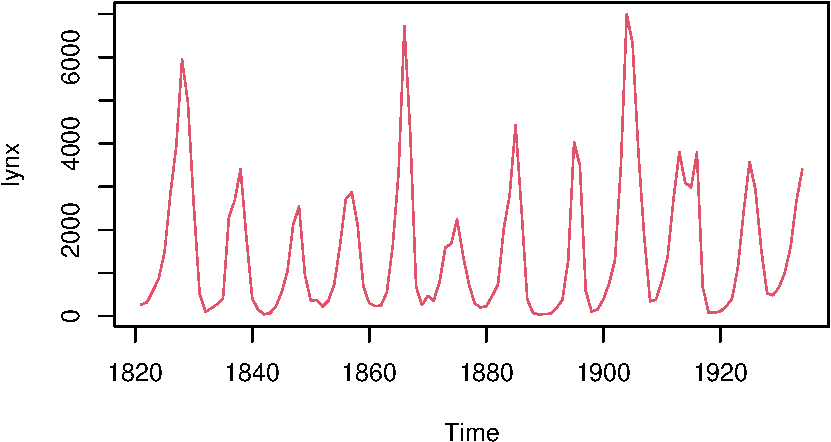
\includegraphics{compbio4all-book_files/figure-latex/unnamed-chunk-8-1.pdf}

\hypertarget{fig.height-5-fig.width-7}{%
\subsection{fig.height = 5, fig.width = 7}\label{fig.height-5-fig.width-7}}

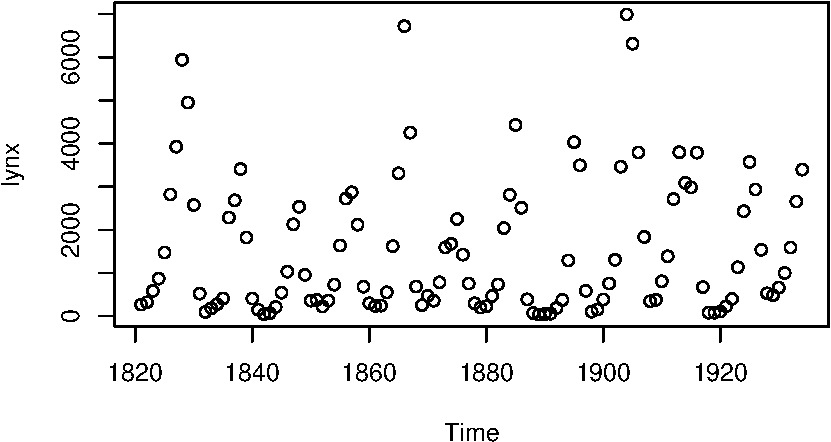
\includegraphics{compbio4all-book_files/figure-latex/unnamed-chunk-9-1.pdf}

\hypertarget{fig.height-4-fig.width-6}{%
\subsection{fig.height = 4, fig.width = 6}\label{fig.height-4-fig.width-6}}

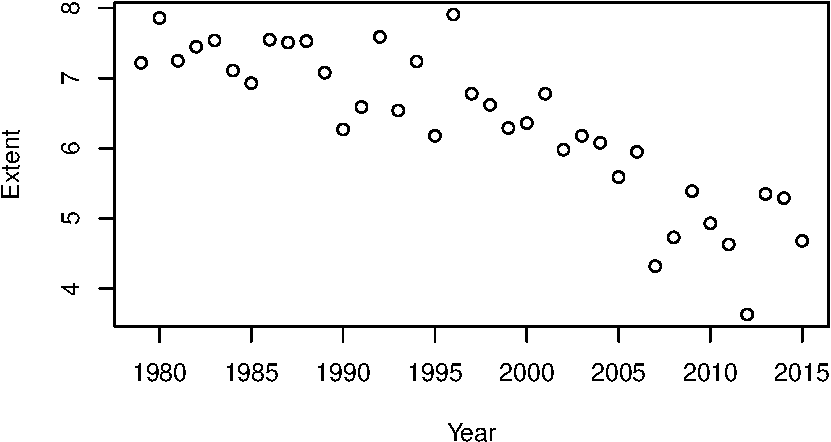
\includegraphics{compbio4all-book_files/figure-latex/unnamed-chunk-10-1.pdf}

\hypertarget{part-introduction}{%
\part{Introduction}\label{part-introduction}}

\hypertarget{predface}{%
\subsection*{Predface}\label{predface}}
\addcontentsline{toc}{subsection}{Predface}

In Book 1 I'll introduce why the role of computers in biology is important and lay out the scope of this book. I'll also walk through the basic steps of getting R and RStudio up and running on your computer, walk through a basic R session, and discuss the various ways we'll interact with R using \textbf{code} and \textbf{script files}. I'll also introduce \textbf{rmarkdown}, a way of integrating the R code of scripts with basic capabilities of word processing and web development. Scripts organized in rmarkdown are a handy way to organize and \textbf{annotate code}, store and disseminate your work, and structure your analyses and data presentations so that the computations behind them are fully \textbf{reproducible}.

\hypertarget{intro}{%
\chapter{Welcome to computational biology for all!}\label{intro}}

Welcome to \emph{Computational Biology for All!}.

This book will introduce you to key concepts of computational biology using the software R. It covers such topics as statistics, data science, bioinformatics, building phylogenetic trees, and building computer models of biological processes.

I will make only two assumptions in this book:

\begin{enumerate}
\def\labelenumi{\arabic{enumi}.}
\tightlist
\item
  You are interested in biology and need a computer to answer a question
\item
  You've had some college-level biology or are willing to read some basic background information in the book, the appendices or the internet.
\end{enumerate}

That's it. If you've forgotten how many amino acids are specified by the genetic code (or never learned; its 20), have never run computer code, or aren't sure what ``computational biology'' is no worries. We'll work through everything step by step, review often, and link to additional resources.

\hypertarget{r-and-rstudio---your-new-best-friends}{%
\section{R and RStudio - your new best friends!}\label{r-and-rstudio---your-new-best-friends}}

\textbf{R} is one of the major computer languages used by scientists. ``R'' refers both to the computer language itself, and to the base software which runs the computer code for us. Most people write and run their code in a special program that acts like a word processor for coding; these goes by the fancy name \textbf{Integrated Development Environments} or \textbf{IDEs}. In this book we'll use the popular IDE software called \textbf{RStudio}.

You should get access to the software combination of the software \textbf{R} and \textbf{RStudio(())} either on the cloud via an account with (\textbf{RStudio Cloud}){[}\url{https://rstudio.cloud/}{]} or on your own hard drive. (Some institutions may have their own special implementation of R and RStudio; ask your tech support about this.)

If your are brand-new to using R the easiest way to get started is using RStudio Cloud. Getting R and RStudio set up on your own computer isn't (usually) difficult, but RStudio Cloud even easier. For information on R, RStudio, and RStudio Cloud see the Appendices. There are also many videos on the internet walking you through these topics.

If I've already lost you a bit with any of this information don't worry - we'll cover more details in the following chapters, and the Appendices cover how to get start with R, RStudio, and RStudio step-by-step.

\hypertarget{how-to-use-this-book---be-an-active-learner}{%
\section{How to use this book - be an active learner!}\label{how-to-use-this-book---be-an-active-learner}}

While you can read this as a regular book, it is meant to be an \textbf{active learning text}. That means you'll get much more out of it if you are working through all the code step by step. There are two ways to do this:

\begin{enumerate}
\def\labelenumi{\arabic{enumi}.}
\tightlist
\item
  Read the book like a book (printed, PDF, website) and type the code in RStudio.
\item
  Download the associated \textbf{Active Learning Notebooks} and work through them in RStudio.
\end{enumerate}

The \textbf{Active Learning Notebooks} contain \textbf{ALL} of the text and code, and is the recommended way to experience the book.

\hypertarget{biological-scope-of-this-book}{%
\section{Biological scope of this book}\label{biological-scope-of-this-book}}

``Computational Biology'' means different things to different people, and I'll discuss how it can be defined in a later chapter. In general, though, I'll apply a very broad definition and touch upon all aspects of biology, from biochemistry to ecology. My starting point will generally by the topics classically associated with computational biology: bioinformatics, genomics, and building phylogenetic trees. Moreover, when I cover other topics like population dynamics or community ecology I'll often use molecular-biology related examples, such as population growth of transposons in our genomes and community diversity of bacteria in our guts (the so-called gut microbiome, which is studied using molecular sequencing technologies). If you're primary interest is in ecology everything in this book will be applicable at the very least in terms of the techniques, and hopefully it will help everyone expand their idea of how ecological concepts can be applied.

\hypertarget{what-is-computational-biology}{%
\chapter{What is Computational Biology?}\label{what-is-computational-biology}}

This is mostly notes.

\hypertarget{notes}{%
\section{Notes}\label{notes}}

\hypertarget{nih-definition}{%
\subsection{NIH definition}\label{nih-definition}}

See file NIH\_def\_bioinfo\_2000.rmd for full text of the NIH document

\textbf{NOTES}:

\begin{itemize}
\tightlist
\item
  bioinformatics relevant to all life sciences (not just biology)
\item
  Bioinf/comp bio both ``rooted'' in life science, comp sci, info sci and technologies
\item
  Bioinformatics: application focused, access / understanding from data
\item
  Comp bio: theory/discovery approaches
\end{itemize}

\begin{quote}
\emph{Bioinformatics:} Research, development, or application of computational tools and approaches for expanding the use of biological, medical, behavioral or health data, including those to acquire, store, organize, archive, analyze, or visualize such data.
\end{quote}

\begin{quote}
\emph{Computational Biology:} The development and application of data-analytical and
theoretical methods, mathematical modeling and computational simulation techniques
to the study of biological, behavioral, and social systems
\end{quote}

\hypertarget{luscombe-et-al-2001}{%
\section{Luscombe et al 2001}\label{luscombe-et-al-2001}}

N.M. Luscombe, D. Greenbaum, M. Gerstein. Bioinformatics definition committee. 2001. What is Bioinformatics? A Proposed Definition and Overview of the Field \url{https://www.thieme-connect.com/products/ejournals/abstract/10.1055/s-0038-1634431}

\begin{quote}
``Our definition is as follows: Bioinformatics is conceptualizing biology in terms of macromolecules (in the sense of physical-chemistry) and then applying ``informatics'' techniques (derived from disciplines such as applied maths, computer science, and statistics) to understand and organize the information associated with these molecules, on a large-scale.'' Luscombe et al 2000
\end{quote}

\begin{quote}
``Analyses in bioinformatics predominantly focus on three types of large datasets available in molecular biology: macromolecular structures, genome sequences, and the results of functional genomics experiments (eg expression data). Additional information includes the text of scientific papers and ``relationship data'' from metabolic pathways, taxonomy trees, and protein-protein interaction networks.'' Luscombe et al 2000
\end{quote}

\hypertarget{taprich-et-al-20121}{%
\section{Taprich et al 20121}\label{taprich-et-al-20121}}

Taprich et al.~2021. An instructional definition and assessment rubric for bioinformatics instruction. \url{https://iubmb.onlinelibrary.wiley.com/doi/full/10.1002/bmb.21361}

\begin{quote}
``An interdisciplinary field that is concerned with the development and application of algorithms that analyze biological data to investigate the structure and function of biological polymers and their relationships to living systems.''
\end{quote}

\hypertarget{smith-2015-frontiers-in-genetics}{%
\section{Smith 2015 Frontiers in Genetics}\label{smith-2015-frontiers-in-genetics}}

Smith. 2015. Broadening the definition of a bioinformatician. Frontiers in Genetics
\url{https://www.frontiersin.org/articles/10.3389/fgene.2015.00258/full}

\begin{quote}
``On a given day, I spend much of my research time staring at nucleotide sequences on a computer screen and theorizing about the evolution of genomes; thus, I feel comfortable calling myself a bioinformatician, or at the very least a scientist who primarily uses bioinformatics for his research. If asked, most of my colleagues, mentors, and students would also define me as a bioinformatician. But there is one small catch: I don't know how to program computer software or curate databases, and I am even quite pathetic at writing UNIX commands, which according to some precludes me from having the title of bioinformatician.'' Smith (2015)
\end{quote}

\begin{quote}
``I imagine that many of the scientists reading this essay will consider me an imposter, an amateur who points, clicks, and stumbles his way through the complicated landscape of bioinformatics. \ldots{} I believe that as a research community we need to broaden our definition of what it means to be a bioinformatician, not restricting it to only those who develop software or design and maintain data resources. \ldots{} {[}T{]}he term bioinformatician should encompass the countless and ever growing number of scientists who use computers and bioinformatics programs to address fundamental questions in biology.'' Smith (2015)
\end{quote}

\hypertarget{good-readings-references}{%
\section{Good readings / references}\label{good-readings-references}}

Koonin, EV. 20xx. Primer: Computational genomics. Current Biology - Magazine. R155-158\ldots{}

\hypertarget{potential-references}{%
\section{Potential references}\label{potential-references}}

\url{https://asistdl.onlinelibrary.wiley.com/doi/full/10.1002/asi.20133?casa_token=iDFXKee8e1gAAAAA\%3AD7vtxphVMi2MHDEIvWi7Y3twQcKUvdI5Co3pF11-OgoTdk1dEHe8H5XKv67mnz1uyGyFRoMeqrbeY_Q}

\url{https://www.geneticsmr.com/sites/default/files/articles/year2017/vol16-1/pdf/gmr-16-01-gmr.16019645_0.pdf}

\url{https://ieeexplore.ieee.org/abstract/document/1678036?casa_token=H9KSAnKN-XIAAAAA:R_uzPueqLDOCWccNZgdRkaRxpOo3J2RSMpVG7ZLAebTVp0-tqGl0TKQderfudEOS2efgl9oWVw}
\url{https://dl.acm.org/doi/abs/10.1145/1031120.1031122?casa_token=YBJzo0bknd8AAAAA:tzp2T3uGqb1MXRPtSccpKXAyKqtmTORa6B_yWGA9dQ9Pj4UElgeH8LK0hVJ_2PaAF51I3oqY8N-EkA}

\hypertarget{original-info-from-eco-data-science-project}{%
\section{Original info, from Eco Data Science project}\label{original-info-from-eco-data-science-project}}

\textbf{{[}NOTE: This section is currently under development. The paper by Touchon \& McCoy (2016) and its references lay out many of the reasons for the statistical focus of this book and relates to all biology, not just ecology.{]}}

\begin{quote}
``Ecological questions and data are becoming increasingly complex and as a result we are seeing the development and proliferation of sophisticated statistical approaches in the ecological literature. \ldots{} It is no longer sufficient to only ask `whether' or `which' experimental manipulations significantly deviate from null expectations. Instead, we are moving toward parameter estimation and asking \textbf{`how much'} and in \textbf{`what direction'} ecological processes are affected by different mechanisms'' (\href{https://esajournals.onlinelibrary.wiley.com/doi/abs/10.1002/ecs2.1394}{Touchon \& McCoy 2016, Ecosphere}, emphsis mine)
\end{quote}

\begin{quote}
``Spreadsheets are often used as the basis of data collection and education; but this is potentially problematic since spreadsheets typically do not promote good data management practices\ldots. The features of spreadsheets that make them desirable for the average researcher, such as extensibility, use of formatting for organization, embedding charts, make them undesirable for preparing data for long‐term archiving and reuse.''(\href{https://esajournals.onlinelibrary.wiley.com/doi/abs/10.1890/ES12-00139.1}{Strasser \& Hampton 2012 Ecosphere})
\end{quote}

\hypertarget{what-is-data-science}{%
\section{What is data science?}\label{what-is-data-science}}

\begin{quote}
Data analysis include ``procedures for analyzing data, techniques for interpreting the results\ldots, ways of planning the gathering of data to make its analysis easier, more precise or more accurate, and all the machinery and results of (mathematical) statistics which apply to analyzing data.'' John Tukey, ``The future of data analysis'', Annals of Mathematical Statistics, 1962.
\end{quote}

\begin{itemize}
\tightlist
\item
  People argue about what data science is
\item
  What Tukey calls ``data analysis'' is now termed ``data science'' by many.\\
\item
  Some define data science as closely allied with computer science and want its use most closely associated with things like ``big data'', data mining, machine learning, and artificial intelligence.
\item
  Others, such as RStudio's Hadley Whickham (creator of ggplot2, dplyr, and most of the infrasture of the tidyverse of R package) define it more broadly to involve all aspects of the life cycle of data.
\item
  (Wickham also defines a data scientists as ``A data scientist is a statistician who is wearing a bow tie'' \url{https://twitter.com/hadleywickham/status/906146116412039169?lang=en})
\end{itemize}

\hypertarget{refereces}{%
\section{Refereces}\label{refereces}}

Strasser \& Hampton 2012. The fractured lab notebook: undergraduates and ecological data management training in the United States. EcoSphere. \url{https://esajournals.onlinelibrary.wiley.com/doi/abs/10.1890/ES12-00139.1}

Touchon \& McCoy 2017. The mismatch between current statistical practice and doctoral training in ecology. EcoSphere. \url{https://esajournals.onlinelibrary.wiley.com/doi/abs/10.1002/ecs2.1394}

Tukey. 1962. The future of data analysis. Annals of Mathematical Statistics. \url{https://www.jstor.org/stable/2237638}

\hypertarget{bibliography}{%
\section{Bibliography}\label{bibliography}}

Relevant papers cited by Touchon \& McOy 2017.

Barraquand, F., T. H. G. Ezard, P. S. Jørgensen, N. Zimmerman, S. Chamberlain, R. Salguero‐Gómez, T. J. Curran, and T. Poisot. 2014. Lack of quantitative training among early‐career ecologists: a survey of the problem and potential solutions. PeerJ 2:e285.

Butcher, J. A., J. E. Groce, C. M. Lituma, M. C. Cocimano, Y. Sánchez‐Johnson, A. J. Campomizzi, T. L. Pope, K. S. Reyna, and A. C. S. Knipps. 2007. Persistent controversy in statistical approaches in wildlife sciences: a perspective of students. Journal of Wildlife Management 71:2142--2144

Ellison, A. M., and B. Dennis. 2009. Paths to statistical fluency for ecologists. Frontiers in Ecology and the Environment 8:362--370.

Germano, J. D. 2000. Ecology, statistics, and the art of misdiagnosis: the need for a paradigm shift. Environmental Reviews 7:167--190.

Quinn, J. F., and A. E. Dunham. 1983. On hypothesis testing in ecology and evolution. American Naturalist 122:602--617.

\hypertarget{how-will-this-book-teach-computational-biology}{%
\chapter{How will this book teach computational biology?}\label{how-will-this-book-teach-computational-biology}}

\begin{quote}
``The rise of computer programming, computational power, and modern statistical approaches may\ldots{}'' allow ``\ldots scientists to ask new questions and to extract more information from data than ever before.'' (\href{https://esajournals.onlinelibrary.wiley.com/doi/abs/10.1002/ecs2.1394}{Touchon \& McCoy 2016, Ecosphere})
\end{quote}

\hypertarget{what-youll-learn}{%
\section{What you'll learn}\label{what-youll-learn}}

\hypertarget{general-skills-that-youll-learn}{%
\subsection{General skills that you'll learn}\label{general-skills-that-youll-learn}}

\begin{itemize}
\tightlist
\item
  \textbf{Statistical computing} using R, RStudio, and rmarkdown
\item
  \textbf{Data analysis}, from t-tests to mixed models in R
\item
  \textbf{Data visualization}, with an emphasis on ggplot2
\item
  \textbf{Data science}, from data management best practices to data cleaning with dplyr
\item
  \textbf{Computational reproducibility}, from formatting scripts to using rmarkdown to write reproducible reports
\end{itemize}

\hypertarget{computational-biology-skills-youll-learn}{%
\subsection{Computational biology skills you'll learn}\label{computational-biology-skills-youll-learn}}

\begin{itemize}
\tightlist
\item
  Working with sequence data
\item
  alignments
\item
  Phylogenetics
\item
  \ldots{}
\end{itemize}

\hypertarget{teaching-approach}{%
\section{Teaching approach}\label{teaching-approach}}

\begin{itemize}
\tightlist
\item
  Always explore and visualize data
\item
  Step-by-step instructions
\item
  Frequently refreshing and review
\item
  Comprehensive and self-contained
\item
  Worked example
\item
  ``Modify this code'' tasks
\item
  Code completion tasks (key steps missing)
\item
  Broken code tasks (fix non-functional code)
\item
  Links to Jupyter notebooks (not yet implemented)
\item
  ``Active Learning Notebooks'' - all content and code in .Rmd format
\end{itemize}

\hypertarget{requirements}{%
\section{Requirements}\label{requirements}}

\begin{itemize}
\tightlist
\item
  R
\item
  RStudio
\item
  External packages loaded via RStudio
\end{itemize}

\hypertarget{whats-not-in-this-book-course}{%
\section{What's not in this book / course}\label{whats-not-in-this-book-course}}

\hypertarget{what-is-r-and-why-use-it}{%
\chapter{What is R and why use it?}\label{what-is-r-and-why-use-it}}

{[}these notes are from a lecture and have not been re-written much yet{]}

R is a powerful piece of software used for data science and data analysis. In this chapter I will briefly introduce the advantages of using R, why you might want to learn it, and also indicate some alternatives and adjuncts you could consider.

\hypertarget{how-do-we-typically-use-software-in-science}{%
\section{How do we typically use software in science?}\label{how-do-we-typically-use-software-in-science}}

Most scientists rely on both general and specialized pieces of software for various parts of their work. For data entry they likely use spreadsheet software Excel, though increasingly Google Sheets. For data analysis they might use one of many options, such as \href{https://www.graphpad.com/}{GraphPad Prism}, Minitab, SAS, SPSS, or STATA. For making plots, many people will export their export their results back to Excel, while others use specialized software like SigmaPlot. Many scientists also use specialized programs; in ecology many researchers do GIS in ArcGIS or QGIS, mark-recapture analysis in Program MARK or Distance, use RAMAS or Vortex for population viability analysis, or build custom mathematical programs in MatLab or Python. If they do \href{https://en.wikipedia.org/wiki/Multivariate_statistics}{multivariate statistics} like {[}ordination{]}(\url{https://en.wikipedia.org/wiki/Ordination_(statistics)} the may use a specialized stats program like PC-ORD.

Since software can be expensive, some scientists will rely on Excel for all of their work. Excel can do many things, but it can't do everything all the specialized types of software can do. Moreover, its very limited in the range of statistics it can do and graphs it can make.

\hypertarget{what-does-r-do}{%
\section{What does R do?}\label{what-does-r-do}}

R is amazing because it has been explicitly developed to do several things very well, particularly statistics, math, making great-looking figures, and writing computer programs to automate these tasks. Additionally, R has been extended by developers to be able to be a powerful tool for data cleaning and organization, to be used as a GIS, and as an integrated word processor and website make for publishing work.

\hypertarget{why-use-r}{%
\section{Why use R}\label{why-use-r}}

In addition to is many capabilities, R has the advantage this it is

\begin{itemize}
\tightlist
\item
  free anyone, always
\item
  used by statisticians to develop new statistical techniques, so new techniques often come out 1st in R
\item
  used by almost all ecological statisticians to develop new techniques (mark recapture, distance sampling)
\end{itemize}

\hypertarget{who-uses-it}{%
\section{Who uses it?}\label{who-uses-it}}

R continues to increase in popularity. Among data scientists it is second only to Python. Among academics it has eclipsed SAS in many fields. It is also used by analyses in many large companies, such Facebook, and by journalists looking for stories in or reporting on large volumes of data

see \url{http://blog.revolutionanalytics.com/2014/05/companies-using-r-in-2014.html} for further discussion.

\hypertarget{r-and-computational-reproducibility}{%
\section{R and computational reproducibility}\label{r-and-computational-reproducibility}}

One factor potentially contributing to R's popularity, or at least a major bonus for using it, is ease of use for making analyses reproducible. All commands in R are typed out and the best way to do this is in a static \textbf{script file} from which you send commands to R to execute. This creates a record of your analyses. This feature is shared by other programs such as SAS and Stats, and other programming languages such as Matlab and Python. The advantage of R is that the script files are simply plain text files which anyone can open and - if they've downloaded R, which is free - they can run. Developers have also created numerous tools for creating \textbf{reproducible analysis workflows} and which allow R to be used in all data-related aspects of a project, from \textbf{data cleaning} to \textbf{formatting journal submissions}. What this means is that without become an expert programmer you can set up your work so that you can re-run all of your data cleaning, analyses, and graph building with a single command in R. This makes what you've done auditable, transparent, and easy to re-use for future work.

\hypertarget{alternatives-to-r}{%
\section{Alternatives to R}\label{alternatives-to-r}}

R has many advantages, but it has one critical issue: the learning curve. R is a command-line driven analysis tool, which means you type out specific commands for almost everything single thing R does. Excel is pretty user friendly, and several stats programs similarly use point-and-click interfaces, such as SPSS, JMP, and Stata SAS also requires a lot of command writing, but is generally consider more user friendly than R.

Recently, two free point-and-click statistical analysis programs have been release that are built on R but require no programming. \href{https://jasp-stats.org/}{JASP} (``Just another statistics program'') has an emphasis on Bayesian statistics, particularly Bayesian hypothesis testing using \href{https://en.wikipedia.org/wiki/Bayes_factor}{Bayes factors} (an approach increasing in popularity, especially in psychology, but which some Bayesians, like Andrew Gelman, \href{http://andrewgelman.com/2011/04/02/so-called_bayes/}{disavow}). While JASP is based on R, it does not currently allow access to the underlying R code.

\href{https://www.jamovi.org/}{Jamovi} has a similar spirit as JASP (indeed, it was founded by developers who had worked on JASP) but is more transparent about the underlying R code being used to run the analysis.

\hypertarget{the-layout-of-rstudio}{%
\chapter{The layout of RStudio}\label{the-layout-of-rstudio}}

To move forward with this book you need to get access to R. There are several ways to do this, and if you are participating in a class your instructor may have a favored way to do it.

\hypertarget{rstudio-desktop-or-cloud}{%
\section{RStudio (Desktop or Cloud)}\label{rstudio-desktop-or-cloud}}

There are two primary ways to use R relevant to this book:

\begin{enumerate}
\def\labelenumi{\arabic{enumi}.}
\tightlist
\item
  \textbf{Create an account at RStudio Cloud.} This is the easiest way to get started; you get 15 hours per month free which is enough for you to get your bearings. Complete instructions for doing this are available in the appendices. Note that RStudio Cloud and RStudio are essentially identical and so all instructions related to RStudio are relevant to RStudio cloud.\\
\item
  \textbf{Download R AND RStudio desktop.} Key here is that you need TWO pieces of software, R and RStudio. Complete instructions are in the appendices.
\end{enumerate}

These two methods are essentially equivalent. To jump in and get started I recommend RStudio cloud. See the appendices for step by step instructions.

\hypertarget{r-emulators}{%
\section{R emulators}\label{r-emulators}}

There are also two other ways of using R which we'll occasionally use. I mention them here briefly. They essentially emulate the R experience but eliminate the hairy details.

\begin{enumerate}
\def\labelenumi{\arabic{enumi}.}
\tightlist
\item
  \textbf{Shiny Apps:} These are independent mini-programs that allow you to explore or carryout some aspect of R functionality without doing any coding. They typically live on the internet, but can also be brought up from RStudio desktop. An example of a simple Shiny App on the internet is \href{https://shiny.rstudio.com/gallery/faithful.html}{here}: \url{https://shiny.rstudio.com/gallery/faithful.html}.
\item
  \textbf{learnr tutorials:} These are interactive tutorials where you do basic coding in your web browser. Here's an example: \url{https://learnr-examples.shinyapps.io/ex-data-filter/}
\end{enumerate}

\hypertarget{other-ways}{%
\section{Other ways}\label{other-ways}}

Two other ways you may encounter R

\begin{enumerate}
\def\labelenumi{\arabic{enumi}.}
\tightlist
\item
  \textbf{Use a Jupyter notebook:} Jupyter notebooks are an advanced R emulator. They are really cool, allowing you to essentially combine text (like a tutorial) with code that can be run within a web browser.\\
\item
  \textbf{Use regular old R:} When you download R an icon will appear on your desktop. You can access old-school R that way, but almost no one ever does. For a bit more information about this see the appendix.
\end{enumerate}

\hypertarget{rstudio-at-a-glance}{%
\section{RStudio at a glance}\label{rstudio-at-a-glance}}

Now we'll get started with RStudio. We'll get to know what it looks like and configure it a bit for out needs.

If you are using RStudio desktop the RStudio logo looks like this:

\begin{figure}

\includegraphics[width=0.79in]{/Users/nlb24/Box Sync/0_R/compbio4all-book/images/RStudio_logo} \caption{The RStudio logo}(\#fig:rstudio.logo)
\end{figure}

Whether on the Cloud or Desktop, when you open up you'll be greeted by a fairly busy array of menus and things. Don't panic! A typical fresh starting point in RStudio/RStudio Cloud is shown in Figure 2.

\begin{figure}
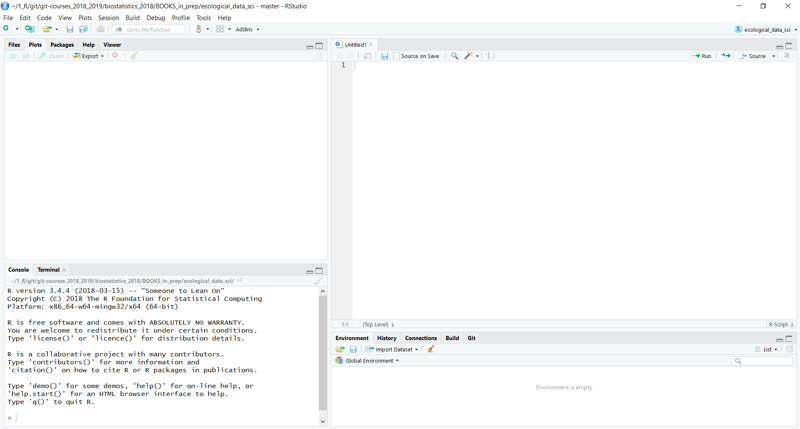
\includegraphics[width=11.11in]{/Users/nlb24/Box Sync/0_R/compbio4all-book/images/RStudio_1st_view-800x600} \caption{RStudio when first opened.}(\#fig:rstudio.open)
\end{figure}

When referring to RStudio (and equivalently RSTudio Cloud - this is the last time I'll mention this so hopefully get get the point), there are two terms that need to be understood. As shown in Figure 3, there is 1)the \textbf{console} section of RStudio and 2) the \textbf{script editor} or \textbf{source viewer}.

\begin{figure}
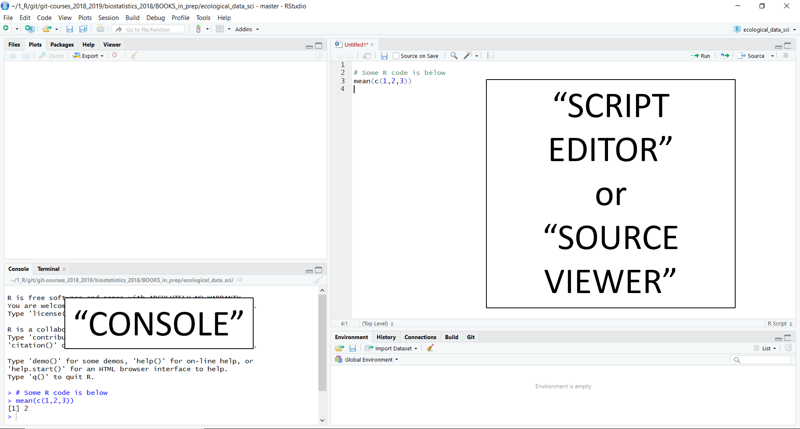
\includegraphics[width=11.11in]{/Users/nlb24/Box Sync/0_R/compbio4all-book/images/RStudio_console_vs_script_editor-800x600} \caption{RStudio's console and script editor.}(\#fig:rstudio.console)
\end{figure}

(A ``cheat sheet'' called the ``RStudio IDE Cheat Sheet'' details all of RStudio's many features and is available at \url{https://www.rstudio.com/resources/cheatsheets/} . It very thorough, though a bit dense. I don't recommend it for beginners but you should remember that it exists.)

\hypertarget{the-console-versus-the-script-editor}{%
\subsection{The console versus the script editor}\label{the-console-versus-the-script-editor}}

You can type and enter text into both the \textbf{console} and the \textbf{script editor} (also called the \textbf{source viewer}. The console, however, responds actively like a calculator, while the script editor works more like a text editor. Information can be passes unidirectionally from the script editor to the console, but not the other way.

\hypertarget{the-r-console}{%
\subsubsection{The R console}\label{the-r-console}}

The \textbf{console} in RStudio gives you \textbf{interactive programming} environment that is very similar to a scientific calculator. If you click your mouse inside the console and type \texttt{1\ +\ 1} then press enter you will see the following type of output

\begin{Shaded}
\begin{Highlighting}[]
\DecValTok{1} \SpecialCharTok{+} \DecValTok{1}
\end{Highlighting}
\end{Shaded}

\begin{verbatim}
## [1] 2
\end{verbatim}

Note that right in front of where you typed \texttt{1+1} there is a \texttt{\textgreater{}} symbol. This is always in the R console and never needs to be typed. You may occasionally see it printed in books or on websites, but it doesn't ever need to be typed.

One thing to note about R is that it's not particular about spacing. All of the following things will yield the same results

\begin{Shaded}
\begin{Highlighting}[]
\DecValTok{1}\SpecialCharTok{+}\DecValTok{1}
\DecValTok{1} \SpecialCharTok{+} \DecValTok{1}
\DecValTok{1}          \SpecialCharTok{+}        \DecValTok{1}
\DecValTok{1} \SpecialCharTok{+}                                   \DecValTok{1}
\end{Highlighting}
\end{Shaded}

Got it? Awesome! Now we're ready for some real data analysis.

\hypertarget{book-getting-started-with-r}{%
\chapter*{(BOOK) Getting started with R}\label{book-getting-started-with-r}}
\addcontentsline{toc}{chapter}{(BOOK) Getting started with R}

\hypertarget{section}{%
\subsection*{}\label{section}}
\addcontentsline{toc}{subsection}{}

\textbf{NEW text}

In Book 2 we'll get started using R. We'll focus on jumping in with some simple examples that tell interesting scientific stories so we can get a sense for the power of R. Later, we'll dig deeper - bit by bit - not the details. Like any language R is a versatile tool for communication, but has conventions, quirks, idioms and dialects that new users have to become comfortable with. In general my goal in Book 2 will be to help you get a general sense of R, let you see a bit of the wild -- and overwhelming -- world of possibilities for how R is written, and outline the more specific aspects I'll use to help facilitate learning.

We'll have three specific goals:

\begin{enumerate}
\def\labelenumi{\arabic{enumi}.}
\tightlist
\item
  Run some initial, simple commands in R to see how it works.
\item
  Take a broad tour of the wide world of R so see the many faces of R code you may encounter in the wild.
\item
  Highlight the particular way coding conventions and idioms of R I'll use.
\item
  Introduce briefly some of the different ways you can get data into R.
\end{enumerate}

If you find yourself getting confused or overwhelmed don't panic A goal of this section is to prevent \emph{future} confusion by giving you a sense for the many different ways R can be written and that you will eventually encounter on the internet or other books, and to contrast them with what you'll use in this book. Here, I've worked to keep things consistent and to either use the simplest methods to accomplish the goal or to carefully break down hard tasks or concepts so you can master them. Once you start typing into your search engine ``R code \ldots{}'' you will get MANY different types of code which you may not yet be prepared to work with.

\hypertarget{hello-r-a-first-encounter-with-data-visualization}{%
\chapter{Hello R! A first encounter with data visualization}\label{hello-r-a-first-encounter-with-data-visualization}}

\hypertarget{key-ideas}{%
\section{Key Ideas}\label{key-ideas}}

\begin{itemize}
\tightlist
\item
  \textbf{Commands}: R uses simple typed commands to do \emph{everything.}
\item
  \textbf{Data}: loading data that comes with R using the \texttt{data()} command.
\item
  \textbf{Plotting}: Making simple plots with the \texttt{plot()} command.
\end{itemize}

\hypertarget{data-in-r}{%
\section{Data in R}\label{data-in-r}}

We'll start our exploration of R with a classic dataset from ecology and statistics showing one of the most striking patterns in wildlife biology: (\textbf{population cycles}){[}\url{https://en.wikipedia.org/wiki/Population_cycle}{]}. Populations are always changing, whether it is declines in the number bacteria in our gut after we take an antibiotic or increases in
raptor species after highly toxic pesticides were banned in the mid-twentieth century.

\begin{figure}
\centering
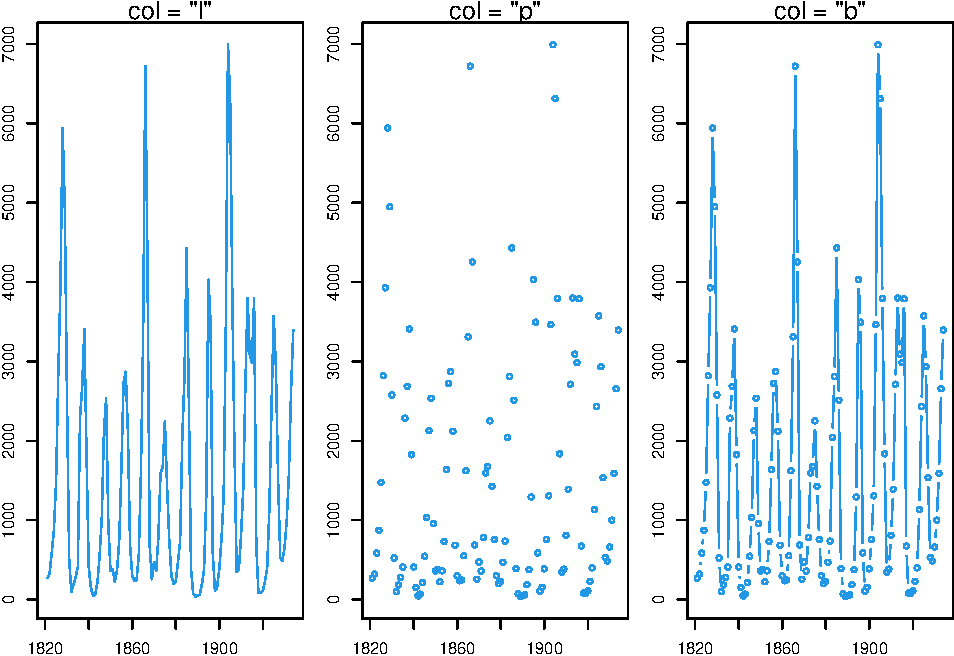
\includegraphics{compbio4all-book_files/figure-latex/unnamed-chunk-13-1.pdf}
\caption{\label{fig:unnamed-chunk-13}Growth of Eagle population in Pennsylvania, USA}
\end{figure}

In stark contrast, a few unique animals populations show dramatic \textbf{oscillations}, with rapid increases soon followed by dramatic drops, as if the population were on a roller coaster. One such population are Canada lynx (\emph{Lynx canadensis}) in Canada.

Lynx are (unfortunately) prized for their soft fur. In years when there are many lynx, trappers kill many lynx; in years when there are few lynx, trappers kill few (however, the number of lynx killed by humans does not contribute to the cycle). Records from fur industry have been compiled by ecologists for over a century to investigate what drives changes in lynx numbers. The table below shows a snapshot of these data, starting from the earliest available records in 1821.

\begin{longtable}[]{@{}
  >{\centering\arraybackslash}p{(\columnwidth - 2\tabcolsep) * \real{0.10}}
  >{\centering\arraybackslash}p{(\columnwidth - 2\tabcolsep) * \real{0.25}}@{}}
\caption{Number of lynx trapped in Canada}\tabularnewline
\toprule
\begin{minipage}[b]{\linewidth}\centering
year
\end{minipage} & \begin{minipage}[b]{\linewidth}\centering
lnyx.population
\end{minipage} \\
\midrule
\endfirsthead
\toprule
\begin{minipage}[b]{\linewidth}\centering
year
\end{minipage} & \begin{minipage}[b]{\linewidth}\centering
lnyx.population
\end{minipage} \\
\midrule
\endhead
1821 & 269 \\
1822 & 321 \\
1823 & 585 \\
1824 & 871 \\
1825 & 1475 \\
1826 & 2821 \\
1827 & 3928 \\
1828 & 5943 \\
1829 & 4950 \\
1830 & 2577 \\
1831 & 523 \\
1832 & 98 \\
1833 & 184 \\
1834 & 279 \\
1835 & 409 \\
\bottomrule
\end{longtable}

You've probably plotted data like this by hand using graph paper, point by point by locating the x-y coordinates. When plotting data like this, time (in this case ``year'') goes on the horizontal \textbf{x-axis}, and the changing variable (lynx.population) goes on the vertical \textbf{y-axis}. In a \textbf{spreadsheet}, you could highlight these columns and click on the ``Make graph'' icons to make the initial plot, then adjust things by clicking on parts of the plot you want to change.

Spreadsheets are said to operate under the principle of \textbf{``What You See Is What You Get''}, or \textbf{WYSIYGY}. They use a fully mouse-drive \textbf{Graphical User Interface (GUI)} where everything is done by pointing and clicking. Every time you make a plot you do these steps.

R is \emph{very} different - you only see things when you want to see them and you do everything via typed commands. This is a large paradigm shift for most people, so we'll start very very slow.

\hypertarget{loading-data-that-comes-with-r}{%
\section{Loading data that comes with R}\label{loading-data-that-comes-with-r}}

The Canada lynx is not just famous with ecologists but also familiar to statisticians who have frequently used it to test statistical methods for studying \textbf{time series} - basically long-term datasets of the same thing. Because of this, these lynx data are embedded within R and easy to access: all you have to do is type \texttt{data(lynx)} into the console and press the ``Enter'' key.

\begin{Shaded}
\begin{Highlighting}[]
\FunctionTok{data}\NormalTok{(lynx)}
\end{Highlighting}
\end{Shaded}

You might be wondering ``\emph{Ok, now what?}'' because nothing apparently happened. What you've done, though is loaded the \texttt{lynx} data into R's active memory, where it will wait for you next command.

Loading your own data into programs such as R can be a pain, so I'll use techniques such as use the \texttt{data()} command to make things as smooth as possible. I'll also introduce other methods, such as loading small datasets using code and downloading them from the internet. I'll also provide a thorough overview in the Appendices.

\hypertarget{plotting-simple-datasets-with-plot}{%
\section{\texorpdfstring{Plotting simple datasets with \texttt{plot()}}{Plotting simple datasets with plot()}}\label{plotting-simple-datasets-with-plot}}

Now in the console type \texttt{plot(lynx)} and press enter. You should see readout like what you see below \ldots{}

\begin{Shaded}
\begin{Highlighting}[]
\FunctionTok{plot}\NormalTok{(lynx)}
\end{Highlighting}
\end{Shaded}

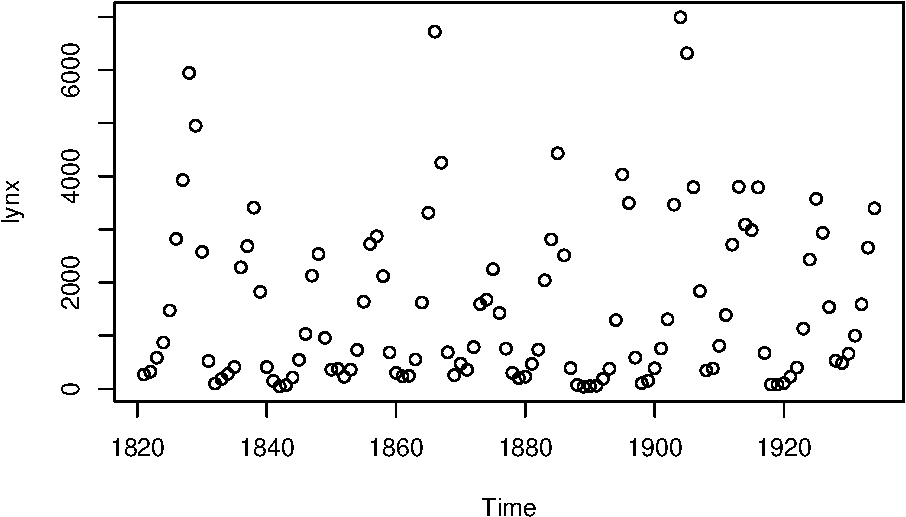
\includegraphics{compbio4all-book_files/figure-latex/unnamed-chunk-16-1.pdf}

\ldots{} and this intriguing plot. The x-axis is time from the early 1800s to the early 1900s, and the y-axis is the number of lynx pelts. This pattern continues to today, and it causes have kept ecologists working hard for over 100 years. Moreover, statistical analyses of data such as these have similarly kept statisticians busy.

This is a simplified example, but that's the basics of working in R:

\begin{enumerate}
\def\labelenumi{\arabic{enumi}.}
\tightlist
\item
  Load data
\item
  Use commands like \texttt{plot} tell R to do something with.
\end{enumerate}

For most of this book we'll use data that's been mostly pre-packaged for you to work with and loaded using the \texttt{data()} command. Real data analyses require more steps, and later in the book we'll briefly cover them so you are familiar with them when you see them elsewhere; further details can also be found in the Appendix.

\hypertarget{commands-in-r}{%
\section{Commands in R}\label{commands-in-r}}

The words ``data'' and ``plot'' in R represent \textbf{commands}; R associates specific code and therefore actions with these words To indicate commands in the text I'll always write it like this: \texttt{data()}. The parentheses are very important in R; forget one of them, and things won't work. After the word representing the command there is always a \textbf{parenthesis} \texttt{(}. Other things such as the name of a dataset go after the first parenthesis, and the command is completed with a matching parenthesis \texttt{)}. To emphasis that things using go within the parentheses I will often write commands like this \texttt{data(...)}, where the \texttt{...} in this case is the name of a dataset.

In some cases you can issue a command, like \texttt{data()}, and R does something only behind the scenes. Often, though, we'll elicit a reaction from R, either data will appear in the Console or a plot will be created.

\hypertarget{the-structure-of-commands-in-r}{%
\section{The structure of commands in R}\label{the-structure-of-commands-in-r}}

Our use of the \texttt{plot()} command was pretty standard; there were two pieces to it:

\begin{enumerate}
\def\labelenumi{\arabic{enumi}.}
\tightlist
\item
  The command, \texttt{plot()}
\item
  The data, \texttt{lynx}
\end{enumerate}

Data in R -- and especially in computational biology -- can take on many forms, which we'll cover as needed as throughout the book. All data is presented in R by an \textbf{object} stored behind the scenes in R's memory. The fact that data in R is usually resting out of view until we do something explicitly with it can take some getting used to, since usually we work with data printed out on a page or displayed in a spreadsheet.

Commands in R almost always include an object within them. Next we'll consider something else that go with commands : \textbf{arguments}.

\hypertarget{arguements-in-r}{%
\section{Arguements in R}\label{arguements-in-r}}

A common mathematical operation when doing data analysis is taking the \textbf{log} of something. (For now we won't worry about what the log is or why we use it' we'll come back to this little bit of math frequently though). We can tell R to plot the log of our lynx data by adding the argument \texttt{log\ =\ "y"} to the \texttt{plot(...)} command. This alters the graph a bit which, for some particular data analysis purposes, will come in handy (more on that later).

\begin{Shaded}
\begin{Highlighting}[]
\FunctionTok{plot}\NormalTok{(lynx, }\AttributeTok{log =} \StringTok{"y"}\NormalTok{)}
\end{Highlighting}
\end{Shaded}

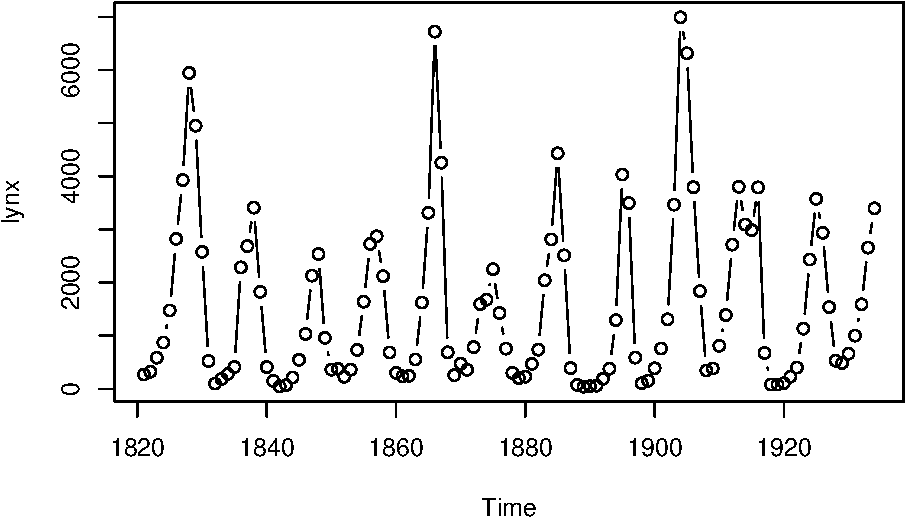
\includegraphics{compbio4all-book_files/figure-latex/unnamed-chunk-17-1.pdf}

In the code above \texttt{log} is the argument and \texttt{"y"} is the \textbf{value} assigned to the argument.

Arguments \textbf{always} have an equals sign with them, so I'll emphasize this by typically writing them as \texttt{argument.name\ =\ ...}. One tricky thing about arguments is that they can take on letters, words, or numbers, and sometimes there need to be quotation marks like \texttt{log\ =\ "y"}, but not always.

Since arguments are fairly tricky, they are a common source of errors, such as forgetting \texttt{=}, or putting the value of the argument in the wrong format.

\hypertarget{arguements-and-more-arguments}{%
\section{Arguements and more arguments}\label{arguements-and-more-arguments}}

We now have three things going on

\begin{enumerate}
\def\labelenumi{\arabic{enumi}.}
\tightlist
\item
  A \textbf{command}, \texttt{plot()}
\item
  A \textbf{data object}, \texttt{lynx}
\item
  An \textbf{argument}, \texttt{log\ =\ "y"}
\end{enumerate}

Most functions in R have multiple arguments that can be invoked Try the following code \texttt{plot(lynx,\ col\ =\ 3)}. That is the \texttt{plot()} function with the argument \texttt{col\ =\ 3} added. What do you think \texttt{col\ =\ 2} means? Try different values like 4, 5, and 6.

\begin{Shaded}
\begin{Highlighting}[]
\FunctionTok{plot}\NormalTok{(lynx, }\AttributeTok{col =} \DecValTok{2}\NormalTok{)}
\end{Highlighting}
\end{Shaded}

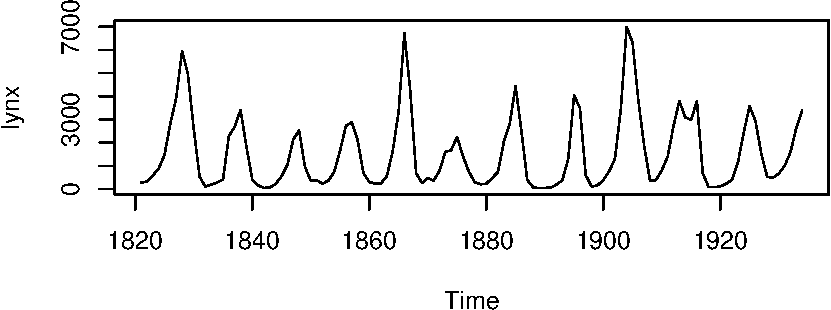
\includegraphics{compbio4all-book_files/figure-latex/unnamed-chunk-18-1.pdf}

Now try this: \texttt{plot(lynx,\ type\ =\ "p")}

Note that there are quotation marks around the p.

\begin{Shaded}
\begin{Highlighting}[]
\FunctionTok{plot}\NormalTok{(lynx, }\AttributeTok{type =} \StringTok{"p"}\NormalTok{)}
\end{Highlighting}
\end{Shaded}

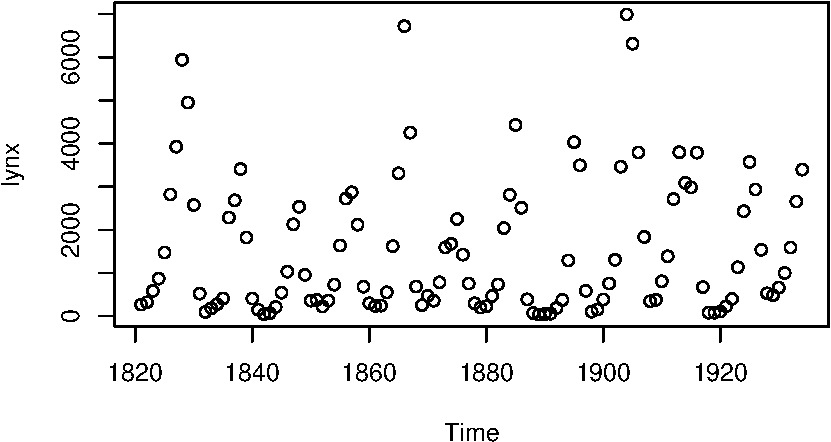
\includegraphics{compbio4all-book_files/figure-latex/unnamed-chunk-19-1.pdf}

Now instead of ``p'' use ``b'', which stands for ``both''. What do you think the ``both'' is referring to?

\begin{Shaded}
\begin{Highlighting}[]
\FunctionTok{plot}\NormalTok{(lynx, }\AttributeTok{type =} \StringTok{"b"}\NormalTok{)}
\end{Highlighting}
\end{Shaded}

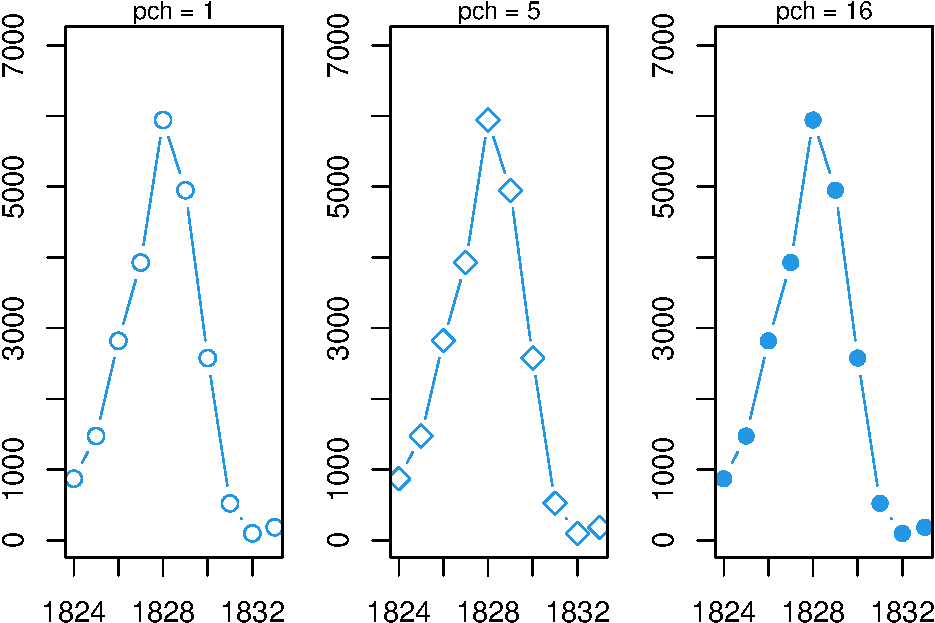
\includegraphics{compbio4all-book_files/figure-latex/unnamed-chunk-20-1.pdf}

\begin{Shaded}
\begin{Highlighting}[]
\DocumentationTok{\#\# }\AlertTok{TODO}\DocumentationTok{: add followup exercises}
\DocumentationTok{\#\#\# R, biology}
\DocumentationTok{\#\# }\AlertTok{TODO}\DocumentationTok{ Add as optional? cover elsewhere}

\FunctionTok{plot}\NormalTok{(}\FunctionTok{log}\NormalTok{(lynx))}
\end{Highlighting}
\end{Shaded}

\hypertarget{multiple-arguments-at-the-same-time}{%
\section{Multiple arguments at the same time}\label{multiple-arguments-at-the-same-time}}

Functions can not only have multiple arguments, but they can \textbf{take on} multiple arguments at the same time. Let's feed two arguments to \texttt{plot()}, \texttt{col\ =\ ...} and a new one, \texttt{type\ =\ ...}.

\begin{Shaded}
\begin{Highlighting}[]
\FunctionTok{plot}\NormalTok{(lynx, }\AttributeTok{col =} \DecValTok{4}\NormalTok{, }\AttributeTok{type =} \StringTok{"b"}\NormalTok{)}
\end{Highlighting}
\end{Shaded}

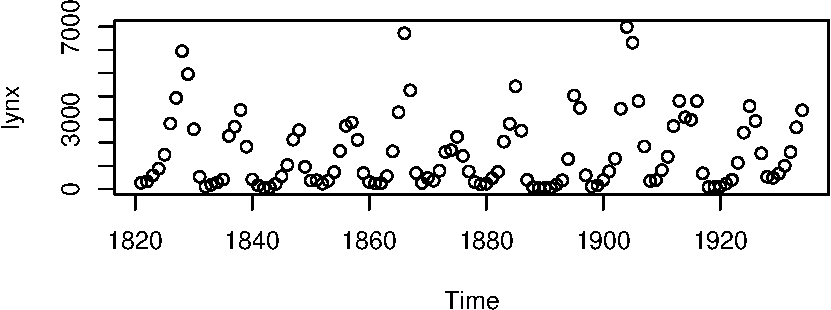
\includegraphics{compbio4all-book_files/figure-latex/unnamed-chunk-22-1.pdf}

Examine the series of plots below; what do you thing \texttt{type=...} is referring to?
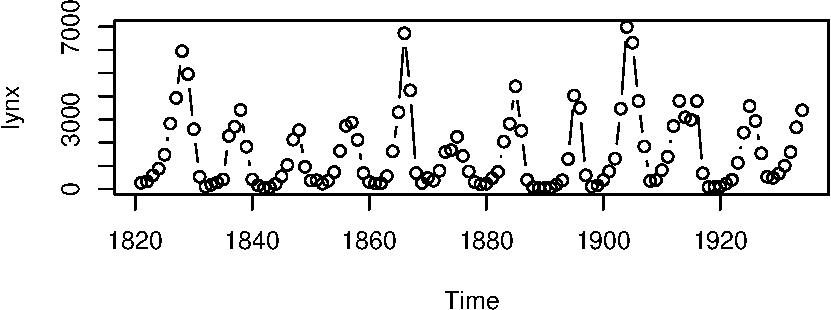
\includegraphics{compbio4all-book_files/figure-latex/unnamed-chunk-23-1.pdf}

\hypertarget{r-commands-and-line-breaks}{%
\section{R commands and line breaks}\label{r-commands-and-line-breaks}}

A cool thing about R is that it doesn't care about \textbf{line breaks} within a command, so I can do this if I want:

\begin{Shaded}
\begin{Highlighting}[]
\FunctionTok{plot}\NormalTok{(lynx, }
     \AttributeTok{col =} \DecValTok{4}\NormalTok{, }
     \AttributeTok{type =} \StringTok{"b"}\NormalTok{)}
\end{Highlighting}
\end{Shaded}

Or if for some reason this

\begin{Shaded}
\begin{Highlighting}[]
\FunctionTok{plot}\NormalTok{(lynx,  }\AttributeTok{col =} \DecValTok{4}\NormalTok{, }
     \AttributeTok{type =} \StringTok{"b"}\NormalTok{)}
\end{Highlighting}
\end{Shaded}

Or even this

\begin{Shaded}
\begin{Highlighting}[]
\FunctionTok{plot}\NormalTok{(lynx,  }
     
     \AttributeTok{col =} \DecValTok{4}\NormalTok{, }
     
     
     \AttributeTok{type =} \StringTok{"b"}\NormalTok{)}
\end{Highlighting}
\end{Shaded}

\hypertarget{code-comments}{%
\section{Code comments}\label{code-comments}}

One thing that putting thing on multiple lines allows you do to is add \textbf{comments} to your code if you place a hashtag (aka pound symbol) in front of it.

\begin{Shaded}
\begin{Highlighting}[]
\FunctionTok{plot}\NormalTok{(lynx,          }\CommentTok{\# data object}
     \AttributeTok{col =} \DecValTok{4}\NormalTok{,       }\CommentTok{\# color argument}
     \AttributeTok{type =} \StringTok{"b"}\NormalTok{)  }\CommentTok{\# type of graph argument}
\end{Highlighting}
\end{Shaded}

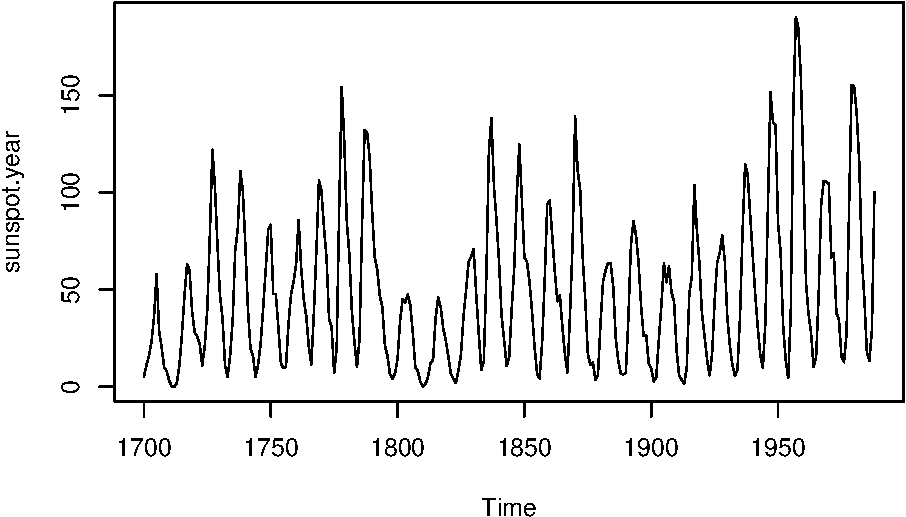
\includegraphics{compbio4all-book_files/figure-latex/unnamed-chunk-27-1.pdf}

\hypertarget{a-note-on-plotting}{%
\section{A note on plotting}\label{a-note-on-plotting}}

One of the great things about R is that it can make really nice plots. You'll soon see that there are many ways to do the same basic thing in R, and this includes making plot. \textbf{Data visualization} is a key aspect of modern science, so its important to build up your skills, including knowing about the different ways plots are made in R. Don't worry though - we'll build all of this up step by step.

\hypertarget{now-you-try-it}{%
\section{Now you try it}\label{now-you-try-it}}

\hypertarget{easy-tasks}{%
\subsection{Easy tasks}\label{easy-tasks}}

Fix each line of code below so the work

\begin{Shaded}
\begin{Highlighting}[]
\NormalTok{plot lynx}
\FunctionTok{plot}\NormalTok{(lynx}
\end{Highlighting}
\end{Shaded}

Examine the plots below. What does \texttt{pch\ =\ ...} do to the plot?
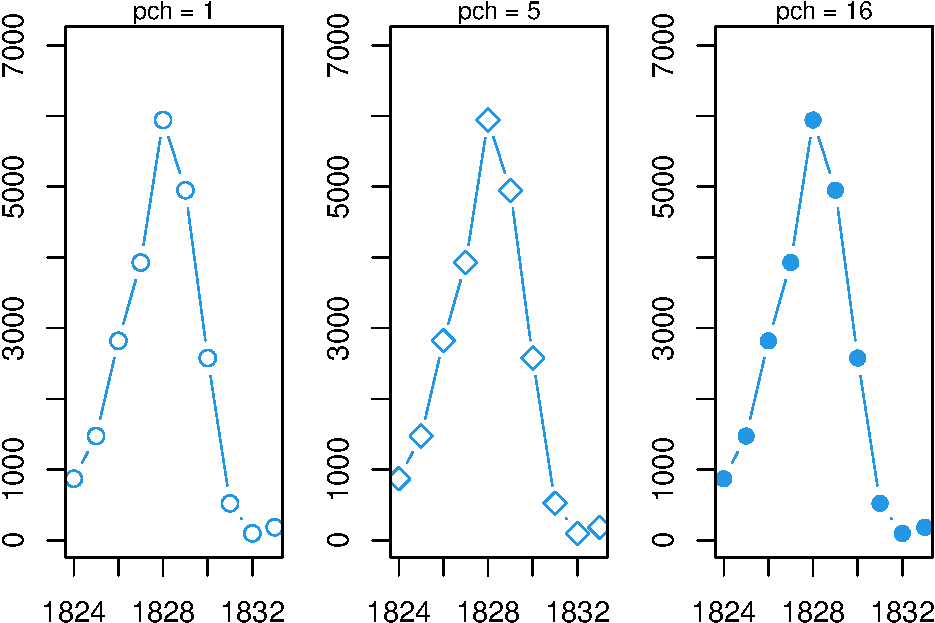
\includegraphics{compbio4all-book_files/figure-latex/unnamed-chunk-30-1.pdf}

Examine the plots below. What does \texttt{lwd\ =\ ...} do to the plot?
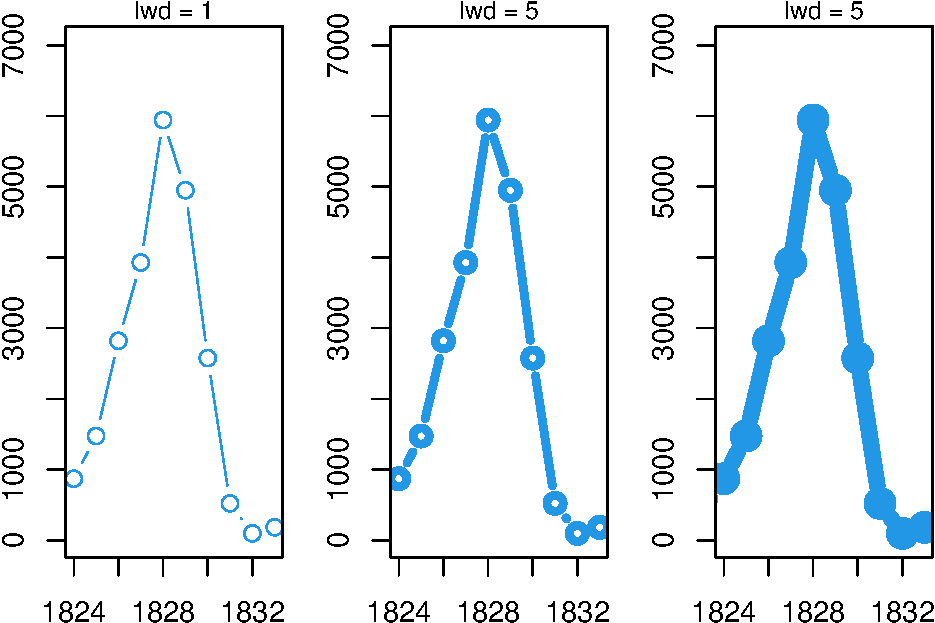
\includegraphics{compbio4all-book_files/figure-latex/unnamed-chunk-31-1.pdf}

Fix each argument below so the code works.

\begin{Shaded}
\begin{Highlighting}[]
\FunctionTok{plot}\NormalTok{(lynx, col  }\DecValTok{1}\NormalTok{)}
\FunctionTok{plot}\NormalTok{(lynx, }\AttributeTok{col =} \StringTok{"1"}\NormalTok{)}
\FunctionTok{plot}\NormalTok{(lynx, type b)}
\FunctionTok{plot}\NormalTok{(lynx, }\AttributeTok{type =}\NormalTok{ b)}
\FunctionTok{plot}\NormalTok{(lynx, type }\StringTok{"b"}\NormalTok{)}
\FunctionTok{plot}\NormalTok{(lynx type }\StringTok{"b"}\NormalTok{)}
\FunctionTok{plot}\NormalTok{(lynx, }\AttributeTok{type =}  \StringTok{"b)}
\end{Highlighting}
\end{Shaded}

\begin{Shaded}
\begin{Highlighting}[]
\FunctionTok{plot}\NormalTok{(lynx, col  }\DecValTok{1}\NormalTok{, }\AttributeTok{type =} \StringTok{"b)}
\StringTok{plot(lynx, col = "}\DecValTok{1}\StringTok{", type = b)}
\StringTok{plot(lynx, pch = 1, type b)}
\StringTok{plot(lynx, pch 1 type = b)}
\StringTok{plot(lynx, lwd = "}\DecValTok{2}\StringTok{" type "}\NormalTok{b}\StringTok{")}
\StringTok{plot(lynx pch = 2, type "}\NormalTok{b}\StringTok{")}
\StringTok{plot(lynx, lwd = 3 type =  "}\NormalTok{b)}
\end{Highlighting}
\end{Shaded}

Split the following code between multiple lines and add a comment between each of them to indicate what the argument does.

\begin{Shaded}
\begin{Highlighting}[]
\FunctionTok{plot}\NormalTok{(lynx, }\AttributeTok{type =} \StringTok{"b"}\NormalTok{, }\AttributeTok{pch =}  \DecValTok{2}\NormalTok{,)}
\end{Highlighting}
\end{Shaded}

\hypertarget{intermediate-tasks}{%
\subsection{Intermediate tasks}\label{intermediate-tasks}}

Here's a challenge: there is another dataset that comes with R called \texttt{sunspot.year} There was once a hypothesized link between the Canada lynx and sunspots that we'll explore later; right now we'll just check it out. See if you can do the following things on your own in the R console.

\hypertarget{make-a-simple-plot}{%
\subsubsection*{Make a simple plot}\label{make-a-simple-plot}}
\addcontentsline{toc}{subsubsection}{Make a simple plot}

\begin{enumerate}
\def\labelenumi{\arabic{enumi}.}
\tightlist
\item
  Using the \texttt{data()} command, load \texttt{sunspot.year} data into R's active memory
\item
  Plot the data.
\end{enumerate}

Your plot should look like this:

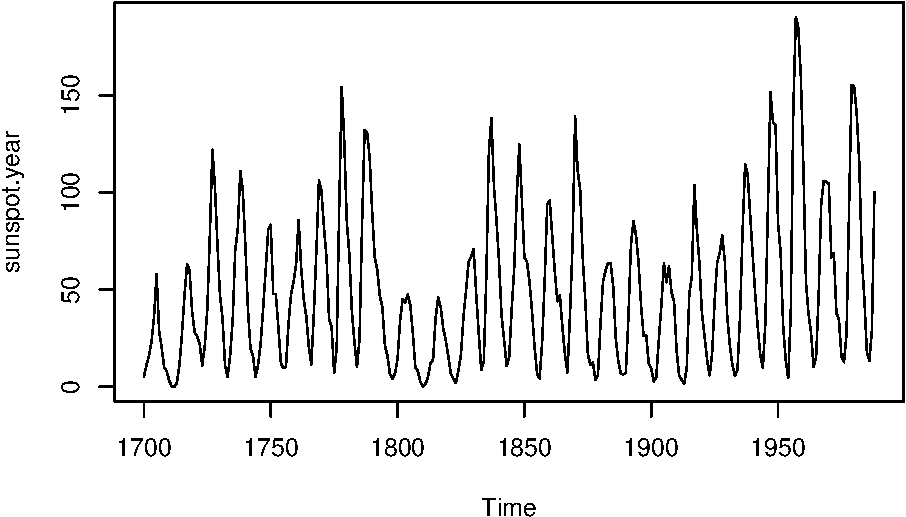
\includegraphics{compbio4all-book_files/figure-latex/unnamed-chunk-37-1.pdf}

\hypertarget{modify-your-plot}{%
\subsubsection*{Modify your plot}\label{modify-your-plot}}
\addcontentsline{toc}{subsubsection}{Modify your plot}

\begin{enumerate}
\def\labelenumi{\arabic{enumi}.}
\tightlist
\item
  Use the \texttt{col\ =} argument to make the color of the line different than black.
\item
  Use the \texttt{type\ =} argument to make the plot show points connected by a line.
\end{enumerate}

Your plot should look like this:

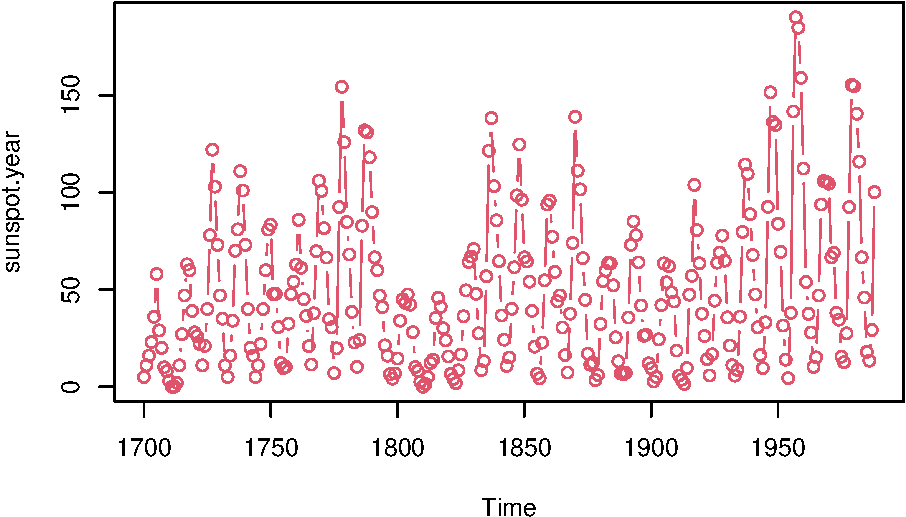
\includegraphics{compbio4all-book_files/figure-latex/unnamed-chunk-38-1.pdf}

\hypertarget{plot-on-the-log-scale}{%
\subsubsection*{Plot on the log scale}\label{plot-on-the-log-scale}}
\addcontentsline{toc}{subsubsection}{Plot on the log scale}

Plot the sunspot data on the log scale. Note: you will get a warnig in red text - you can ignore this.

\begin{verbatim}
## Warning in xy.coords(x, NULL, log = log, setLab = FALSE): 3 y values <= 0
## omitted from logarithmic plot
\end{verbatim}

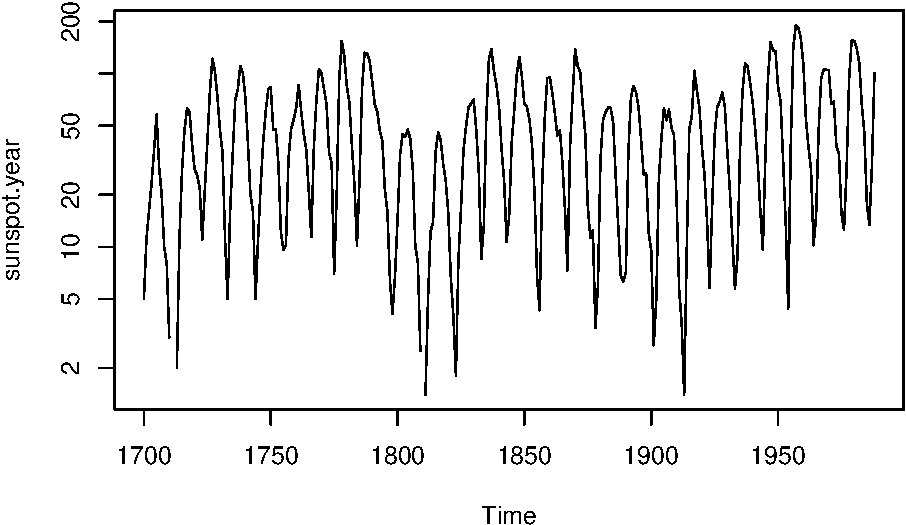
\includegraphics{compbio4all-book_files/figure-latex/unnamed-chunk-39-1.pdf}

\hypertarget{downloading-r-packages-and-their-data}{%
\chapter{Downloading R packages (and their data)}\label{downloading-r-packages-and-their-data}}

In the previous chapter we used some data the comes with R. In this lesson we'll start expanding out from the \textbf{Base R distribution} and exploring the ways that external \textbf{packages} extend R.

\hypertarget{loading-data-from-r-packages}{%
\section{Loading data from R packages}\label{loading-data-from-r-packages}}

\textbf{NEW text:}
When you install R you get *Base R**, which is the core set of functions, functionality, and some data sets. Base R is surrounded by a universe of extensions built by statistician, programmers, academics and businesses that use R for analyses. A lot of R's functionality is found in these packages, including data sets, special plotting functions, and statistical tools for the analysis of complex data. These have to be downloaded from the internet and installed. Most packages contain data in order to demonstrate what they do.

Most R packages you'll use are stored on the CRAN website where you download R (\url{https://cran.r-project.org/}). R and RStudio have functions and tools for downloading and managing packages that we'll briefly introduce in this exercise.

Another major platform for packages is called \textbf{Bioconductor}; we'll cover downloading packages from there later. Finally, many packages are hosted on a site called \textbf{GitHub}. This book relies heavily on an R package I've written and hosted on GitHub called \texttt{combio4all} (\url{https://brouwern.github.io/combio4all/}) that contains the datasets used throughout the book, as well as some helpful R functions I've written. Many packages on CRAN also occur on GitHub, especially if programmers are actively developing, updating, and managing the package. We'll cover downloading packages from GitHub later.

\hypertarget{functions-arguements}{%
\subsection{Functions \& Arguements}\label{functions-arguements}}

\begin{itemize}
\tightlist
\item
  \texttt{install.packages()}

  \begin{itemize}
  \tightlist
  \item
    Argument: \texttt{dependencies\ =\ TRUE}
  \end{itemize}
\item
  \texttt{library()}
\end{itemize}

\begin{center}\rule{0.5\linewidth}{0.5pt}\end{center}

\hypertarget{optional-what-functions-come-with-base-r}{%
\section{OPTIONAL: What functions come with base R?}\label{optional-what-functions-come-with-base-r}}

\textbf{The following section is OPTIONAL}

If for some reason you want to see \emph{all} the functions that come with the distribution base R, type this into the console and press enter. (\texttt{ls} stands for ``list'' and is a function we'll use more later).

\begin{Shaded}
\begin{Highlighting}[]
\CommentTok{\# this code chunk is OPTIONAL}
\FunctionTok{ls}\NormalTok{(}\StringTok{"package:base"}\NormalTok{)}
\end{Highlighting}
\end{Shaded}

As R has been developed there has also built up a cannon of tried and true packages that are downloaded automatically when you download R. If you want to see all of the packages that come with base R, do this. \texttt{library()} is a function you will use a lot.

\begin{Shaded}
\begin{Highlighting}[]
\CommentTok{\# this code chunk is OPTIONAL}
\FunctionTok{.libPaths}\NormalTok{(}\StringTok{""}\NormalTok{) }
\FunctionTok{library}\NormalTok{()}
\end{Highlighting}
\end{Shaded}

One package that is part of this cannon is \texttt{MASS}, which stands for Modern Applied Statistics in S. ``S'' is the precursor to R, and MASS is the package that accompanies the book of the same name, which is one of the original books on S/R. (\url{https://www.springer.com/us/book/9780387954578})

\textbf{End OPTIONAL section}

\begin{center}\rule{0.5\linewidth}{0.5pt}\end{center}

\hypertarget{load-data-from-an-external-r-package}{%
\section{Load data from an external R package}\label{load-data-from-an-external-r-package}}

Many packages have to be explicitly downloaded and installed in order to use their functions and datasets. Note that this is a \textbf{two-step process}:

\begin{enumerate}
\def\labelenumi{\arabic{enumi}.}
\tightlist
\item
  Download package from internet with \texttt{install.packages(...)}
\item
  Explicitly tell R to load it with \texttt{library(...)}
\end{enumerate}

\hypertarget{step-1-downloading-packages-install.packages...}{%
\subsection{\texorpdfstring{Step 1: Downloading packages \texttt{install.packages(...)}}{Step 1: Downloading packages install.packages(...)}}\label{step-1-downloading-packages-install.packages...}}

There are a number of ways to install packages. One of the easiest is to use the function \texttt{install.packages()}. Note that it might be better to call this ``download.packages'' since after you download it, you still have to load it! (Lots of confusion has resulted from calling this function ``install.packages'').

We'll download a package with lots of interesting biology data called \texttt{Stat2Data}. Note that in the \textbf{call} to \texttt{install.packages(...)}, the name of the package is in quotes.

\begin{Shaded}
\begin{Highlighting}[]
\FunctionTok{install.packages}\NormalTok{(}\StringTok{"Stat2Data"}\NormalTok{)}
\end{Highlighting}
\end{Shaded}

Often when you download a package you'll see a fair bit of red text. Usually there's nothing of interest here, but sometimes you need to read over it for hints about why something didn't work.

For example, when I downloaded this package I got this cryptic message in bright red text:
\texttt{trying\ URL\ \textquotesingle{}https://cran.rstudio.com/bin/macosx/contrib/4.0/Stat2Data\_2.0.0.tgz\textquotesingle{}}
\texttt{Content\ type\ \textquotesingle{}application/x-gzip\textquotesingle{}\ length\ 1177728\ bytes\ (1.1\ MB)}
\texttt{==================================================}
\texttt{downloaded\ 1.1\ MB}

Followed by this in less insistent black:
\texttt{The\ downloaded\ binary\ packages\ are\ in}
\texttt{/var/folders/q8/gwjfr69n05vf4h15l6hdl4d8x1zk5v/T//RtmpeRHx2y/downloaded\_packages}

This is all perfectly normal, so don't worry.

\hypertarget{protip-dont-re-download-packages-all-the-time}{%
\subsubsection{Protip: don't re-download packages all the time}\label{protip-dont-re-download-packages-all-the-time}}

You can think of R and RStudio like a computer operating systems, and packages like software you chose to download. R, RStudio and packages will need to be updated at times - indeed, the first step in diagnosing many problems with R is to update things. But updates probably only need to be done every six months or so at the most; I generally wait until things stop working.

Anytime a lesson introduces a new package I'll include code to do the download. You only need to do this once unless you start encountering a problems. A way to make this happen is to \textbf{comment out} the code by putting a hashtag in front of it like this

\begin{Shaded}
\begin{Highlighting}[]
\CommentTok{\# install.packages("Stat2Data")}
\end{Highlighting}
\end{Shaded}

This preserves the code but tells R \emph{``don't run this line.''}

\hypertarget{step-2-explicitly-loading-a-package}{%
\subsection{Step 2: Explicitly loading a package}\label{step-2-explicitly-loading-a-package}}

The \texttt{install.packages()} function just downloads the package software to R; now you need to tell R explicitly \emph{``I want to work with the package''}. This is done using the \texttt{library()} function. (Its called library because another name for packages is \textbf{libraries}. ).

\begin{Shaded}
\begin{Highlighting}[]
\FunctionTok{library}\NormalTok{(Stat2Data)}
\end{Highlighting}
\end{Shaded}

As frequently is the case, R doesn't look like its doing much, but you've actually just installed a bunch of cool datasets.

In contrast to running \texttt{install.packages()}, \texttt{library()} need to be run \textbf{every time you use the code}. More specifically, every time you re-start R. What happens is when you shut down R, all the packages you loaded using \texttt{library()} are taken out of memory. Next time you use R you need to re-load them using \texttt{libary()}.

\begin{center}\rule{0.5\linewidth}{0.5pt}\end{center}

\hypertarget{optional-seeing-all-of-your-installed-packages}{%
\section{OPTIONAL: Seeing all of your installed packages}\label{optional-seeing-all-of-your-installed-packages}}

\textbf{The following section is OPTIONAL}

If for some reason you want to see everything you've downloaded, do this.

\begin{Shaded}
\begin{Highlighting}[]
\CommentTok{\# This code is optional}
\FunctionTok{installed.packages}\NormalTok{()}
\end{Highlighting}
\end{Shaded}

\textbf{End OPTIONAL section}

\begin{center}\rule{0.5\linewidth}{0.5pt}\end{center}

\hypertarget{downloading-packages-using-rstudio}{%
\section{Downloading packages using RStudio}\label{downloading-packages-using-rstudio}}

RStudio has a point-and-click interface to download packages. In the pane of the RStudio GUI that says ``Files, Plots, Packages, Help, Viewer'' click on ``Packages''. Below ``Packages'' it will then say ``Install, Update, ..,'' Click on ``Install.'' (There might be a lag during this process as RStudio gets info about your packages). In the pop up widow there will be a middle field ``Packages'' where you can type the name of the package you need. There's an auto-complete feature to help you in case you forget the name. Then click ``install.'' Note that in the bottom right corner of the pop up is a checked box next to ``Install dependencies.'' Leave that checked; more on that later.

This is a useful function, but I don't do this very often because I include any download information in my scripts.

\hypertarget{your-turn}{%
\section{Your turn}\label{your-turn}}

Fix this code

\begin{Shaded}
\begin{Highlighting}[]
\FunctionTok{install.packages}\NormalTok{(MASS)}
\FunctionTok{install.packages}\NormalTok{(}\StringTok{"car)}
\StringTok{install.packages ggplot2 }
\StringTok{install.packages(cowplot }
\StringTok{install.packagesggpubr }
\end{Highlighting}
\end{Shaded}

The package \texttt{carData} contains a time series dataset called USpop. Fix the following code to download and plot these data.

\begin{Shaded}
\begin{Highlighting}[]
\FunctionTok{install.packages}\NormalTok{(}\StringTok{"carData"}\NormalTok{)}
\FunctionTok{plot}\NormalTok{(USPop)}
\end{Highlighting}
\end{Shaded}

The package \texttt{boot} contains a dataset called \texttt{ducks} on the behavior of crosses between two species of ducks: Mallards and Pintails Fix the following code to download and plot these data.

\begin{Shaded}
\begin{Highlighting}[]
\FunctionTok{install.packages}\NormalTok{(}\StringTok{"boot"}\NormalTok{)}
\FunctionTok{library}\NormalTok{(boot)}
\FunctionTok{plot}\NormalTok{(ducks)}
\end{Highlighting}
\end{Shaded}

\hypertarget{data-in-dataframes}{%
\chapter{Data in dataframes}\label{data-in-dataframes}}

\begin{Shaded}
\begin{Highlighting}[]
\FunctionTok{library}\NormalTok{(Stat2Data)}
\end{Highlighting}
\end{Shaded}

An interesting dataset in \texttt{Stat2Data} is \texttt{SeaIce}. Load it with the \texttt{data()} command.

\begin{Shaded}
\begin{Highlighting}[]
\FunctionTok{data}\NormalTok{(SeaIce)}
\end{Highlighting}
\end{Shaded}

\texttt{SeaIce} shows 37 years of the area of frozen ice in the arctic, from 1979 to 1993. The \texttt{lynx} data we worked with previously was in a special format that you'll probably rarely encounter ever again. It was nice to use, however, because it required very little code to plot.\\
SeaIce, however, is a typical R data object in the form of a \textbf{dataframe}. Dataframes are fundamental units of analysis in R. Most of the data you will load into R and work within R will be in a dataframe. The have the same basic structure as a spreadsheet, but R keeps them hidden in memory and you have to use commands to explore them.

\hypertarget{looking-at-dataframes-with-view}{%
\subsection{\texorpdfstring{Looking at dataframes with \texttt{View()}}{Looking at dataframes with View()}}\label{looking-at-dataframes-with-view}}

To get a spreadsheet-like view of a dataframe you can use the \texttt{View} command

\begin{Shaded}
\begin{Highlighting}[]
\FunctionTok{View}\NormalTok{(SeaIce)}
\end{Highlighting}
\end{Shaded}

This will bring up the data in a spreadsheet like viewer as a new tab in the script editor, similar to this.

\begin{longtable}[]{@{}
  >{\centering\arraybackslash}p{(\columnwidth - 6\tabcolsep) * \real{0.10}}
  >{\centering\arraybackslash}p{(\columnwidth - 6\tabcolsep) * \real{0.12}}
  >{\centering\arraybackslash}p{(\columnwidth - 6\tabcolsep) * \real{0.10}}
  >{\centering\arraybackslash}p{(\columnwidth - 6\tabcolsep) * \real{0.10}}@{}}
\toprule
\begin{minipage}[b]{\linewidth}\centering
Year
\end{minipage} & \begin{minipage}[b]{\linewidth}\centering
Extent
\end{minipage} & \begin{minipage}[b]{\linewidth}\centering
Area
\end{minipage} & \begin{minipage}[b]{\linewidth}\centering
t
\end{minipage} \\
\midrule
\endhead
1979 & 7.22 & 4.54 & 1 \\
1980 & 7.86 & 4.83 & 2 \\
1981 & 7.25 & 4.38 & 3 \\
1982 & 7.45 & 4.38 & 4 \\
1983 & 7.54 & 4.64 & 5 \\
1984 & 7.11 & 4.04 & 6 \\
1985 & 6.93 & 4.18 & 7 \\
1986 & 7.55 & 4.67 & 8 \\
1987 & 7.51 & 5.61 & 9 \\
1988 & 7.53 & 5.32 & 10 \\
\bottomrule
\end{longtable}

⚠️ \textbf{Note:} Unlike a spreadsheet you cannot edit the data when is called up using \texttt{View()} ⚠️

Like a spreadsheet the data are organized in columns and rows. Each \textbf{column} represents a type of information:

\begin{itemize}
\tightlist
\item
  \texttt{Year}: when data were collected
\item
  \texttt{Extent}: the amount of area within the ice-bound region
\item
  \texttt{Area}: total area of ice, minus any non-ice area (land, melted water)
\item
  \texttt{t}: time point, from 1 (1979) to 15 (1993)
\end{itemize}

You can think of \texttt{Extent} as similar to the size of a country, and \texttt{Area} as the actual amount of land in a country minus any lakes.

Each row represents a different year of data; row 1 is the \texttt{Extent} and \texttt{Area} for 1979, row to is the \texttt{Extent} and \texttt{Area} for 1980 and so on.

\hypertarget{looking-at-dataframes-in-the-console}{%
\subsection{Looking at dataframes in the console}\label{looking-at-dataframes-in-the-console}}

Another common way to examine data is simply type the name of the data in the console and press enter. This prints it out; however, if its a large data frame this may take up a LOT of room. (I'll just show an exert here).

\begin{Shaded}
\begin{Highlighting}[]
\NormalTok{SeaIce}
\end{Highlighting}
\end{Shaded}

\begin{verbatim}
##    Year Extent Area  t
## 1  1979   7.22 4.54  1
## 2  1980   7.86 4.83  2
## 3  1981   7.25 4.38  3
## 4  1982   7.45 4.38  4
## 5  1983   7.54 4.64  5
## 6  1984   7.11 4.04  6
## 7  1985   6.93 4.18  7
## 8  1986   7.55 4.67  8
## 9  1987   7.51 5.61  9
## 10 1988   7.53 5.32 10
## 11 1989   7.08 4.83 11
## 12 1990   6.27 4.51 12
## 13 1991   6.59 4.47 13
## 14 1992   7.59 5.38 14
## 15 1993   6.54 4.53 15
\end{verbatim}

\hypertarget{plotting-data-in-dataframes}{%
\chapter{Plotting data in dataframes}\label{plotting-data-in-dataframes}}

\begin{Shaded}
\begin{Highlighting}[]
\FunctionTok{library}\NormalTok{(Stat2Data)}
\FunctionTok{data}\NormalTok{(SeaIce)}
\end{Highlighting}
\end{Shaded}

Most data in R are organized into dataframes. Similar to when we plot data in a spreadsheet, to plot data from a dataframe we need to tell R exactly what we want on the \textbf{x-axis (horizontal)} and \textbf{y-axis (vertical)}.

⚠️ \textbf{Note:} For reasons we don't have to get in to, the \texttt{lynx} data were a special case where we didn't have to define x and y⚠️

We can plot the Extent of artic sea ice again using the \texttt{plot()} command, and using a cool convention in R called \textbf{formula notation}. Formula notation uses the (\textbf{tilde}){[}\url{https://en.wikipedia.org/wiki/Tilde}{]} symbol \texttt{\textasciitilde{}}. In math, \texttt{\textasciitilde{}} can have several meanings. In R, it means ``relates to'' , ``versus'', ``depends on.'' So we can plot the relation between \texttt{Year} and seac \texttt{Extent} as a \textbf{y versus x} relation as \texttt{Extent\ \textasciitilde{}\ Year}. We also have to include the argument \texttt{data\ =\ SeaIce} so R knows where to get \texttt{Extent} and \texttt{Year}.

\begin{Shaded}
\begin{Highlighting}[]
\FunctionTok{plot}\NormalTok{(Extent }\SpecialCharTok{\textasciitilde{}}\NormalTok{ Year, }\AttributeTok{data =}\NormalTok{ SeaIce)  }\CommentTok{\# Note, both words capitalized.}
\end{Highlighting}
\end{Shaded}

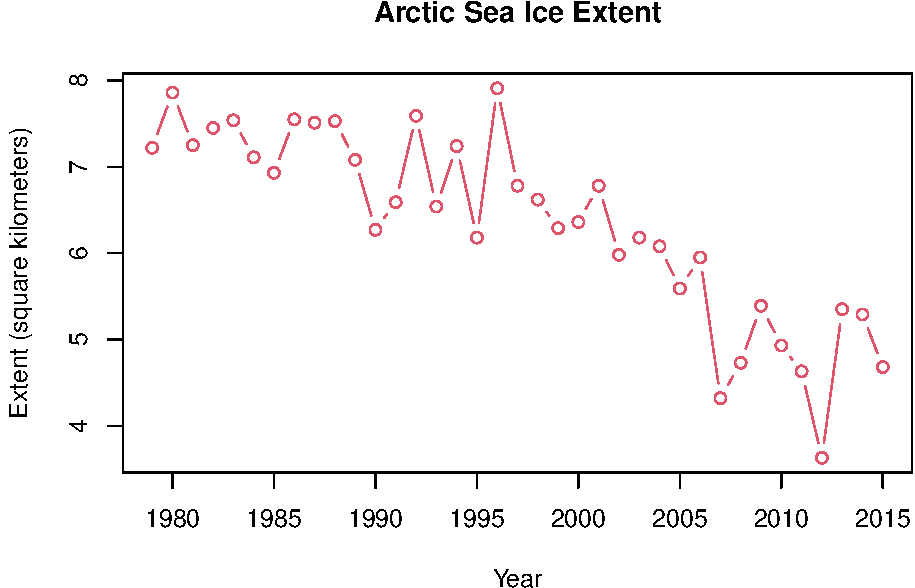
\includegraphics{compbio4all-book_files/figure-latex/unnamed-chunk-58-1.pdf}

\hypertarget{base-r-graphics}{%
\section{Base-R graphics}\label{base-r-graphics}}

When we use the \texttt{plot} command were using \textbf{Base R} graphics. As noted before there are several ways to make plots in R and you should be able to spot which one is which when looking at code. We'll cover some of the key features of Bare R graphics now. While different plotting methods have different commands and arguments, they all share a common feature: everything in a plot can be customized, and each element is customized with a command or arguement.

\hypertarget{type-of-points}{%
\subsection{Type of points}\label{type-of-points}}

\texttt{plot()} can draw dots or lines We make it use lines using the \texttt{type\ =\ "l"} argument (note that the l is in quotes)

\begin{Shaded}
\begin{Highlighting}[]
\FunctionTok{plot}\NormalTok{(Extent }\SpecialCharTok{\textasciitilde{}}\NormalTok{ Year, }\AttributeTok{type =} \StringTok{"l"}\NormalTok{, }\AttributeTok{data =}\NormalTok{ SeaIce)  }\CommentTok{\# Note: l in quotes}
\end{Highlighting}
\end{Shaded}

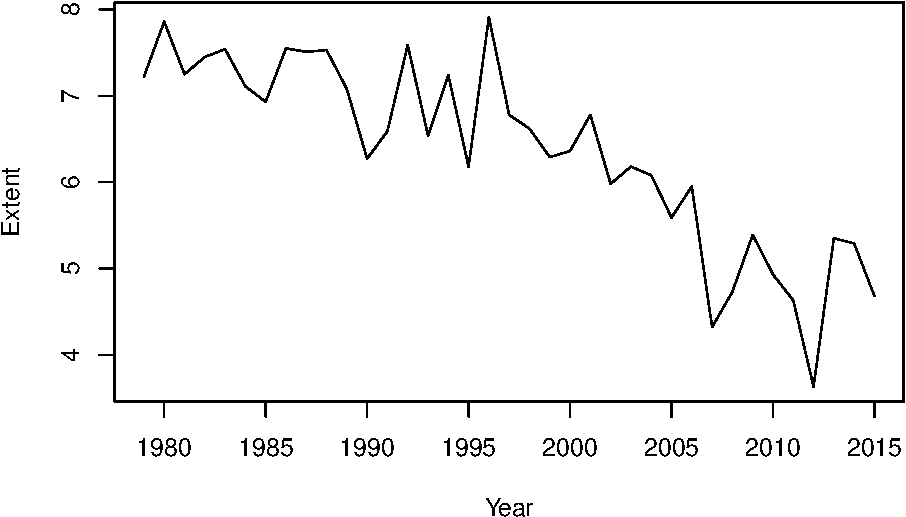
\includegraphics{compbio4all-book_files/figure-latex/unnamed-chunk-59-1.pdf}

As noted before, R doesn't mind if you split things on lines. To keep track of the things I''m doing to the plot I'll format things like this

\begin{Shaded}
\begin{Highlighting}[]
\FunctionTok{plot}\NormalTok{(Extent }\SpecialCharTok{\textasciitilde{}}\NormalTok{ Year,  }\CommentTok{\# relationship}
     \AttributeTok{type =} \StringTok{"l"}\NormalTok{,     }\CommentTok{\# type of plot; Note: l in quotes}
     \AttributeTok{data =}\NormalTok{ SeaIce)  }\CommentTok{\# data}
\end{Highlighting}
\end{Shaded}

As we did with the \texttt{lynx} data we can combine points and lines with \texttt{type\ =\ "b"}. (Do you recall what ``b'' stands for?)

\begin{Shaded}
\begin{Highlighting}[]
\FunctionTok{plot}\NormalTok{(Extent }\SpecialCharTok{\textasciitilde{}}\NormalTok{ Year,  }\CommentTok{\# relationship}
     \AttributeTok{type =} \StringTok{"b"}\NormalTok{,     }\CommentTok{\# type of plot; Note: b in quotes}
     \AttributeTok{data =}\NormalTok{ SeaIce)  }\CommentTok{\# data}
\end{Highlighting}
\end{Shaded}

We can adjust color with \texttt{col\ =\ ...}. Recall the this is just a number, not in quotes.

\begin{Shaded}
\begin{Highlighting}[]
\FunctionTok{plot}\NormalTok{(Extent }\SpecialCharTok{\textasciitilde{}}\NormalTok{ Year,  }\CommentTok{\# relationship}
     \AttributeTok{type =} \StringTok{"b"}\NormalTok{,     }\CommentTok{\# type of plot; Note: b in quotes}
     \AttributeTok{col =} \DecValTok{2}\NormalTok{,        }\CommentTok{\# color; no quotes}
     \AttributeTok{data =}\NormalTok{ SeaIce)  }\CommentTok{\# data}
\end{Highlighting}
\end{Shaded}

We can add a main title to with \texttt{main\ =\ ...}

\begin{Shaded}
\begin{Highlighting}[]
\FunctionTok{plot}\NormalTok{(Extent }\SpecialCharTok{\textasciitilde{}}\NormalTok{ Year,  }\CommentTok{\# relationship}
     \AttributeTok{type =} \StringTok{"b"}\NormalTok{,     }\CommentTok{\# type of plot; Note: b in quotes}
     \AttributeTok{col =} \DecValTok{2}\NormalTok{,        }\CommentTok{\# color; no quotes}
     \AttributeTok{main =} \StringTok{"Arctic Sea Ice Extent"}\NormalTok{, }\CommentTok{\# main title, in quotes}
     \AttributeTok{data =}\NormalTok{ SeaIce)  }\CommentTok{\# data}
\end{Highlighting}
\end{Shaded}

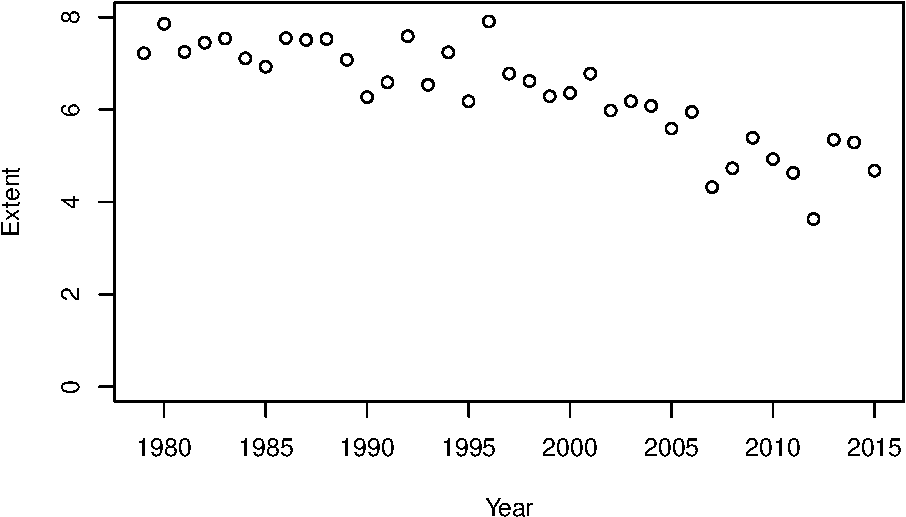
\includegraphics{compbio4all-book_files/figure-latex/unnamed-chunk-63-1.pdf}

Its always good to include your units. \texttt{Extent} and \texttt{Area} are in square kilometers. We can say specifically what we want for the y-axis label using \texttt{ylab\ =\ ...}

\begin{Shaded}
\begin{Highlighting}[]
\FunctionTok{plot}\NormalTok{(Extent }\SpecialCharTok{\textasciitilde{}}\NormalTok{ Year,  }\CommentTok{\# relationship}
     \AttributeTok{type =} \StringTok{"b"}\NormalTok{,     }\CommentTok{\# type of plot; Note: b in quotes}
     \AttributeTok{col =} \DecValTok{2}\NormalTok{,        }\CommentTok{\# color; no quotes}
     \AttributeTok{main =} \StringTok{"Arctic Sea Ice Extent"}\NormalTok{, }\CommentTok{\# main title, in quotes}
     \AttributeTok{ylab =} \StringTok{"Extent (square kilometers)"}\NormalTok{,}
     \AttributeTok{data =}\NormalTok{ SeaIce)  }\CommentTok{\# data}
\end{Highlighting}
\end{Shaded}

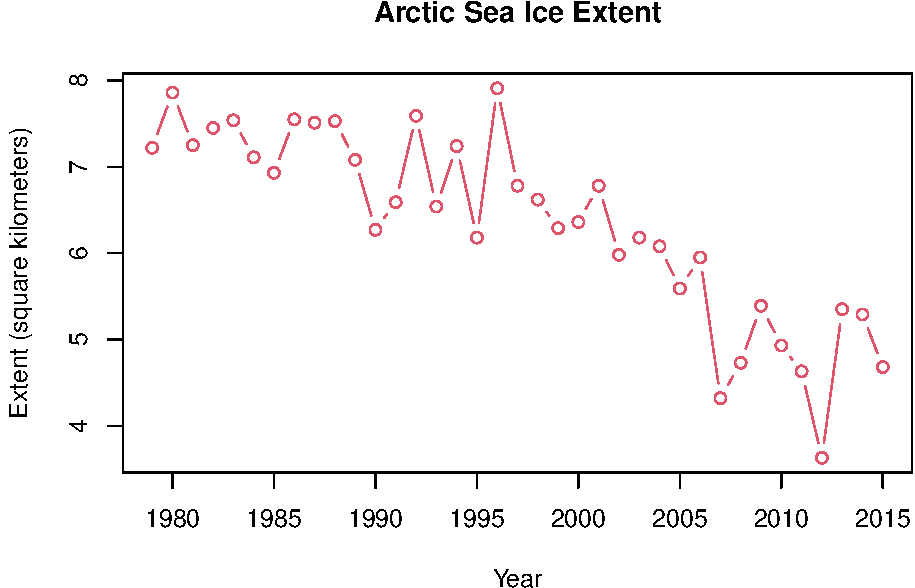
\includegraphics{compbio4all-book_files/figure-latex/unnamed-chunk-64-1.pdf}

We can change the appearance of the line using \texttt{lty\ =\ ...}, which stands for ``line type'':

\begin{Shaded}
\begin{Highlighting}[]
\FunctionTok{plot}\NormalTok{(Extent }\SpecialCharTok{\textasciitilde{}}\NormalTok{ Year,  }\CommentTok{\# relationship}
     \AttributeTok{type =} \StringTok{"b"}\NormalTok{,     }\CommentTok{\# type of plot; Note: b in quotes}
     \AttributeTok{col =} \DecValTok{2}\NormalTok{,        }\CommentTok{\# color; no quotes}
     \AttributeTok{main =} \StringTok{"Arctic Sea Ice Extent"}\NormalTok{, }\CommentTok{\# main title, in quotes}
     \AttributeTok{ylab =} \StringTok{"Extent (square kilometers)"}\NormalTok{,}
     \AttributeTok{lty =} \DecValTok{2}\NormalTok{,        }\CommentTok{\# line type; not quoted}
     \AttributeTok{data =}\NormalTok{ SeaIce)  }\CommentTok{\# data}
\end{Highlighting}
\end{Shaded}

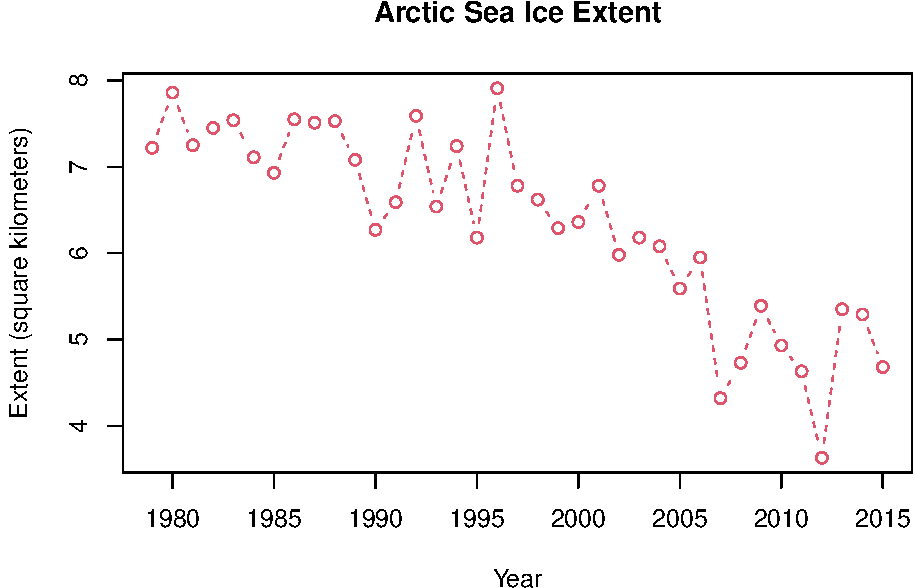
\includegraphics{compbio4all-book_files/figure-latex/unnamed-chunk-65-1.pdf}

I'm not a fan of the open circles for plotting points; we can change those too using the argument \texttt{pch\ =}.

\begin{Shaded}
\begin{Highlighting}[]
\FunctionTok{plot}\NormalTok{(Extent }\SpecialCharTok{\textasciitilde{}}\NormalTok{ Year,  }\CommentTok{\# relationship}
     \AttributeTok{type =} \StringTok{"b"}\NormalTok{,     }\CommentTok{\# type of plot; Note: b in quotes}
     \AttributeTok{col =} \DecValTok{2}\NormalTok{,        }\CommentTok{\# color; no quotes}
     \AttributeTok{main =} \StringTok{"Arctic Sea Ice Extent"}\NormalTok{, }\CommentTok{\# main title, in quotes}
     \AttributeTok{ylab =} \StringTok{"Extent (square kilometers)"}\NormalTok{,}
     \AttributeTok{lty =} \DecValTok{2}\NormalTok{,        }\CommentTok{\# line type; not quoted}
     \AttributeTok{pch =} \DecValTok{16}\NormalTok{,       }\CommentTok{\# point type; not quoted}
     \AttributeTok{data =}\NormalTok{ SeaIce)  }\CommentTok{\# data}
\end{Highlighting}
\end{Shaded}

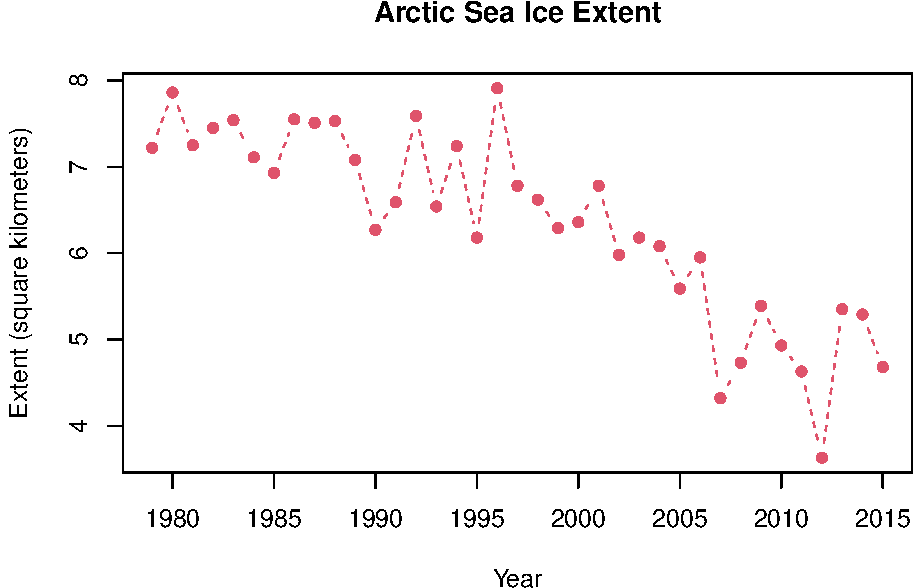
\includegraphics{compbio4all-book_files/figure-latex/unnamed-chunk-66-1.pdf}

\hypertarget{plotting-two-columns-of-data}{%
\subsection{Plotting two columns of data}\label{plotting-two-columns-of-data}}

Often we want to represent two distinct things on our graph. In spreadsheets these are called separate \textbf{series} of data. When making a \textbf{time series plot} like this one we can add a new column of data using a species command called \texttt{points()} which works very similar to \texttt{plot()}.

⚠️ \textbf{Note:} The \texttt{points()} command only works if its it precede by a statement from the \texttt{plot()} command ⚠️

\begin{Shaded}
\begin{Highlighting}[]
\CommentTok{\# Main plot: Extent}
\FunctionTok{plot}\NormalTok{(Extent }\SpecialCharTok{\textasciitilde{}}\NormalTok{ Year,  }\CommentTok{\# relationship}
     \AttributeTok{type =} \StringTok{"b"}\NormalTok{,     }\CommentTok{\# type of plot; Note: b in quotes}
     \AttributeTok{col =} \DecValTok{2}\NormalTok{,        }\CommentTok{\# color; no quotes}
     \AttributeTok{main =} \StringTok{"Arctic Sea Ice Extent"}\NormalTok{, }\CommentTok{\# main title, in quotes}
     \AttributeTok{ylab =} \StringTok{"Extent (square kilometers)"}\NormalTok{,}
     \AttributeTok{lty =} \DecValTok{2}\NormalTok{,        }\CommentTok{\# line type; not quoted}
     \AttributeTok{pch =} \DecValTok{16}\NormalTok{,       }\CommentTok{\# point type; not quoted}
     \AttributeTok{data =}\NormalTok{ SeaIce)  }\CommentTok{\# data}

\CommentTok{\# Second column of data: Area}
\FunctionTok{points}\NormalTok{(Area }\SpecialCharTok{\textasciitilde{}}\NormalTok{ Year, }\AttributeTok{data =}\NormalTok{ SeaIce)}
\end{Highlighting}
\end{Shaded}

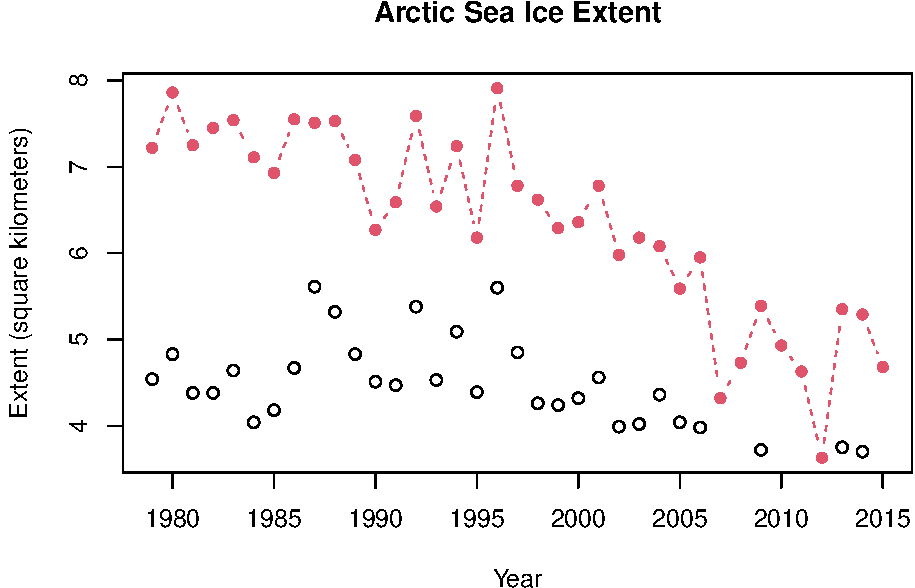
\includegraphics{compbio4all-book_files/figure-latex/unnamed-chunk-67-1.pdf}

I can now customize the sea ice \texttt{Area} part of the plot by add \textbf{arguements} to the \texttt{points()} statement.

\begin{Shaded}
\begin{Highlighting}[]
\CommentTok{\# Main plot: Extent}
\FunctionTok{plot}\NormalTok{(Extent }\SpecialCharTok{\textasciitilde{}}\NormalTok{ Year,  }\CommentTok{\# relationship}
     \AttributeTok{type =} \StringTok{"b"}\NormalTok{,     }\CommentTok{\# type of plot; Note: b in quotes}
     \AttributeTok{col =} \DecValTok{2}\NormalTok{,        }\CommentTok{\# color; no quotes}
     \AttributeTok{main =} \StringTok{"Arctic Sea Ice Extent"}\NormalTok{, }\CommentTok{\# main title, in quotes}
     \AttributeTok{ylab =} \StringTok{"Extent (square kilometers)"}\NormalTok{,}
     \AttributeTok{lty =} \DecValTok{2}\NormalTok{,        }\CommentTok{\# line type; not quoted}
     \AttributeTok{pch =} \DecValTok{16}\NormalTok{,       }\CommentTok{\# point type; not quoted}
     \AttributeTok{data =}\NormalTok{ SeaIce)  }\CommentTok{\# data}

\CommentTok{\# Second column of data: Area}
\FunctionTok{points}\NormalTok{(Area }\SpecialCharTok{\textasciitilde{}}\NormalTok{ Year,}
       \AttributeTok{type =} \StringTok{"b"}\NormalTok{,}
       \AttributeTok{col =} \DecValTok{3}\NormalTok{,}
       \AttributeTok{pch =} \DecValTok{17}\NormalTok{,}
       \AttributeTok{data =}\NormalTok{ SeaIce)}
\end{Highlighting}
\end{Shaded}

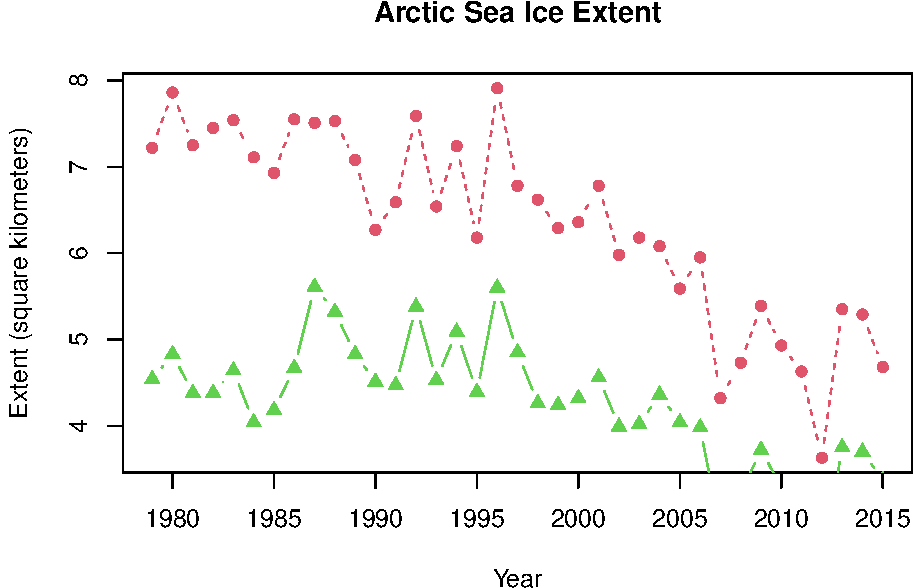
\includegraphics{compbio4all-book_files/figure-latex/unnamed-chunk-68-1.pdf}

❓ There's a problem with my graph though - can you spot it? It only really becomes apparent when you connect the dots with a line. ❓

\hypertarget{changing-the-range-of-a-plot-axis}{%
\subsection{Changing the range of a plot axis}\label{changing-the-range-of-a-plot-axis}}

Let's go back to our original plot and forget about all the fancy arguments and adding \texttt{points()} for a little bit. The problem with the last graph we made is that some points are not showing - if you look in the lower right-hand part points around 2006-2008 and 2011-2013 are not showing up because the y-axis stops around 3.5. We can fix this by adding a new argument which sets the limits of the y-axis: \texttt{ylim\ =\ ...}. To do this correctly, we have to introduce a new function: \texttt{c()}. This is actually one of the most common functions in R. In the \texttt{c()} we need to tell R the lower and upper limits we want for the y-axis. Let's do 0 and 8, which will be coded as \texttt{c(0,8)}.

So, to set the y-axis limits we do this:

\begin{Shaded}
\begin{Highlighting}[]
\FunctionTok{plot}\NormalTok{(Extent }\SpecialCharTok{\textasciitilde{}}\NormalTok{ Year,  }
     \AttributeTok{ylim =} \FunctionTok{c}\NormalTok{(}\DecValTok{0}\NormalTok{,}\DecValTok{8}\NormalTok{), }\CommentTok{\# the c(...) fucntion to set limits}
     \AttributeTok{data =}\NormalTok{ SeaIce) }
\end{Highlighting}
\end{Shaded}

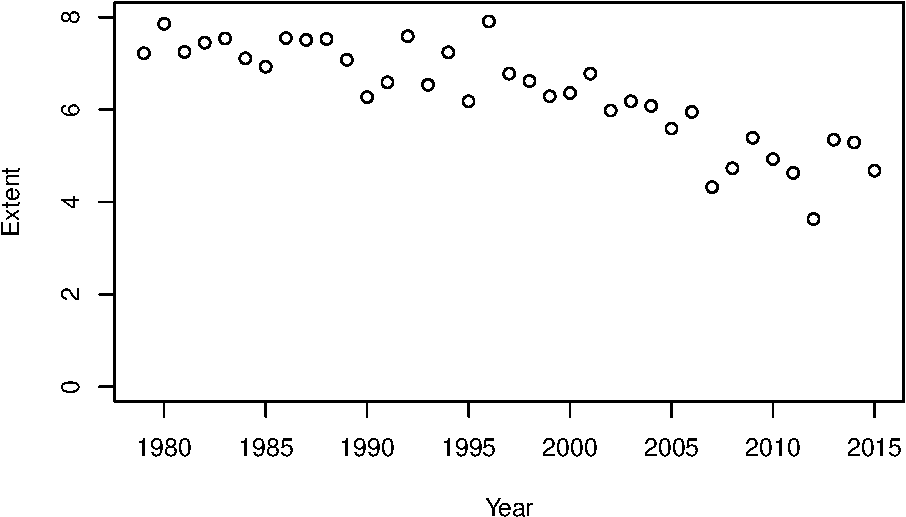
\includegraphics{compbio4all-book_files/figure-latex/unnamed-chunk-69-1.pdf}

Now we have a bunch more space at the bottom. We can add our \texttt{points()} back to see if this work:

\begin{Shaded}
\begin{Highlighting}[]
\FunctionTok{plot}\NormalTok{(Extent }\SpecialCharTok{\textasciitilde{}}\NormalTok{ Year,  }
     \AttributeTok{ylim =} \FunctionTok{c}\NormalTok{(}\DecValTok{0}\NormalTok{,}\DecValTok{8}\NormalTok{), }\CommentTok{\# the c(...) fucntion to set limits}
     \AttributeTok{data =}\NormalTok{ SeaIce) }
\FunctionTok{points}\NormalTok{(Area }\SpecialCharTok{\textasciitilde{}}\NormalTok{ Year,}
      \AttributeTok{data =}\NormalTok{ SeaIce,}
      \AttributeTok{col =} \DecValTok{2}\NormalTok{)}
\end{Highlighting}
\end{Shaded}

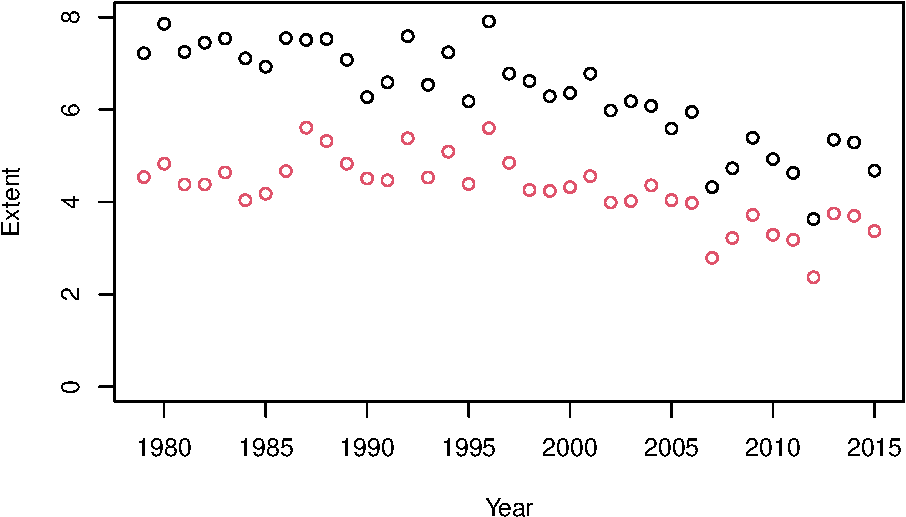
\includegraphics{compbio4all-book_files/figure-latex/unnamed-chunk-70-1.pdf}

⚠️ \textbf{Note:} \texttt{ylim\ =\ ...} only goes in \texttt{plot()}, not \texttt{points()}. \texttt{View()} ⚠️

Let's re-make our fancy plots now with \texttt{ylim\ =\ ...} set.

\begin{Shaded}
\begin{Highlighting}[]
\CommentTok{\# Main plot: Extent}
\FunctionTok{plot}\NormalTok{(Extent }\SpecialCharTok{\textasciitilde{}}\NormalTok{ Year,  }
     \AttributeTok{type =} \StringTok{"b"}\NormalTok{,     }
     \AttributeTok{col =} \DecValTok{2}\NormalTok{,       }
     \AttributeTok{main =} \StringTok{"Arctic Sea Ice Extent"}\NormalTok{, }
     \AttributeTok{ylab =} \StringTok{"Extent (square kilometers)"}\NormalTok{,}
     \AttributeTok{lty =} \DecValTok{2}\NormalTok{,        }
     \AttributeTok{pch =} \DecValTok{16}\NormalTok{,       }
     \AttributeTok{ylim =} \FunctionTok{c}\NormalTok{(}\DecValTok{0}\NormalTok{,}\DecValTok{8}\NormalTok{), }\CommentTok{\# \textless{}\#\textless{}== y{-}axis limits}
     \AttributeTok{data =}\NormalTok{ SeaIce)  }

\CommentTok{\# Second column of data: Area}
\FunctionTok{points}\NormalTok{(Area }\SpecialCharTok{\textasciitilde{}}\NormalTok{ Year,}
       \AttributeTok{type =} \StringTok{"b"}\NormalTok{,}
       \AttributeTok{col =} \DecValTok{3}\NormalTok{,}
       \AttributeTok{pch =} \DecValTok{17}\NormalTok{,}
       \AttributeTok{data =}\NormalTok{ SeaIce)}
\end{Highlighting}
\end{Shaded}

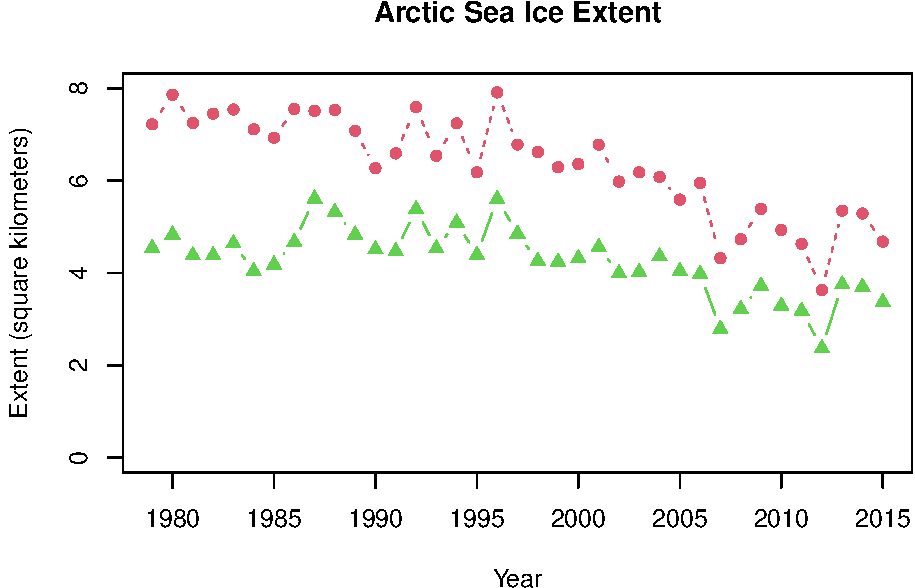
\includegraphics{compbio4all-book_files/figure-latex/unnamed-chunk-71-1.pdf}

\hypertarget{you-try-it}{%
\section{You try it}\label{you-try-it}}

\hypertarget{fixer-uppers}{%
\subsection{Fixer-uppers}\label{fixer-uppers}}

Fix the code below so it works

\begin{Shaded}
\begin{Highlighting}[]
\FunctionTok{plot}\NormalTok{(Extent , Year,  }
     \AttributeTok{data =}\NormalTok{ SeaIce)  }
\end{Highlighting}
\end{Shaded}

Fix the code below so it works

\begin{Shaded}
\begin{Highlighting}[]
\FunctionTok{plot}\NormalTok{(Extent }\SpecialCharTok{\textasciitilde{}}\NormalTok{ Year,  }\CommentTok{\# relationship}
     \AttributeTok{type =}\NormalTok{ b,     }\CommentTok{\# type of plot; Note: b in quotes}
     \AttributeTok{col =} \StringTok{"2"}\NormalTok{,        }\CommentTok{\# color; no quotes}
     \AttributeTok{data =}\NormalTok{ SeaIce)  }\CommentTok{\# data}
\end{Highlighting}
\end{Shaded}

\hypertarget{intermediate}{%
\subsection{Intermediate}\label{intermediate}}

Make a plot with \texttt{Area} on the x-axis and \texttt{Extent} on the y-axis.

\begin{Shaded}
\begin{Highlighting}[]
\DocumentationTok{\#\# Write the code below}
\end{Highlighting}
\end{Shaded}

\hypertarget{advanced}{%
\subsection{Advanced}\label{advanced}}

Based on the code above, make a plot of the SeaIce data where \texttt{Area} appears within the \texttt{plot()} statement, and \texttt{Extent} is in \texttt{points()}.

\begin{Shaded}
\begin{Highlighting}[]
\CommentTok{\# Write the code below: }
\end{Highlighting}
\end{Shaded}

\hypertarget{build-your-own-dataframe-part-i-vectors}{%
\chapter{Build your own dataframe part I: Vectors}\label{build-your-own-dataframe-part-i-vectors}}

\hypertarget{dataframes-are-a-type-of-data-structure}{%
\section{Dataframes are a type of data structure}\label{dataframes-are-a-type-of-data-structure}}

For small datasets its often useful to build your own dataframes. Dataframes are \textbf{objects} in R; in particular they are a type of \textbf{data structure}. ``Data structure'' is just a fancy way of saying ``holding or organizing data.''

We'll work with the \texttt{SeaIce} data again.

\begin{Shaded}
\begin{Highlighting}[]
\FunctionTok{library}\NormalTok{(Stat2Data)}
\FunctionTok{data}\NormalTok{(}\StringTok{"SeaIce"}\NormalTok{)}
\end{Highlighting}
\end{Shaded}

If we're curious about what kind of data is in an object we can use the \texttt{class()} command to see how is is classified.. Generally the first thing R spits out is the most important.

\begin{Shaded}
\begin{Highlighting}[]
\FunctionTok{class}\NormalTok{(SeaIce)}
\end{Highlighting}
\end{Shaded}

\begin{verbatim}
## [1] "data.frame"
\end{verbatim}

We see that \texttt{SeaIce\ is\ a}data.frame`.

A related command is \texttt{is()}

\begin{Shaded}
\begin{Highlighting}[]
\FunctionTok{is}\NormalTok{(SeaIce)}
\end{Highlighting}
\end{Shaded}

\begin{verbatim}
## [1] "data.frame" "list"       "oldClass"   "vector"
\end{verbatim}

This command is more \textbf{verbose} and tells of several things, the most relevant of which is that \texttt{SeaIce} is a dataframe.

The \texttt{SeaIce} dataframe has several columns. We can pull up their names using the \texttt{names()} command.

\begin{Shaded}
\begin{Highlighting}[]
\FunctionTok{names}\NormalTok{(SeaIce)}
\end{Highlighting}
\end{Shaded}

\begin{verbatim}
## [1] "Year"   "Extent" "Area"   "t"
\end{verbatim}

There are times when we may want to examine just a single column. We can isolate a single column using a species notation which uses a dollar sign. To get the \texttt{Extent} column we do this

\begin{Shaded}
\begin{Highlighting}[]
\NormalTok{SeaIce}\SpecialCharTok{$}\NormalTok{Extent}
\end{Highlighting}
\end{Shaded}

\begin{verbatim}
##  [1] 7.22 7.86 7.25 7.45 7.54 7.11 6.93 7.55 7.51 7.53 7.08 6.27 6.59 7.59 6.54
## [16] 7.24 6.18 7.91 6.78 6.62 6.29 6.36 6.78 5.98 6.18 6.08 5.59 5.95 4.32 4.73
## [31] 5.39 4.93 4.63 3.63 5.35 5.29 4.68
\end{verbatim}

\hypertarget{dataframes-are-made-from-vectors}{%
\section{Dataframes are made from vectors}\label{dataframes-are-made-from-vectors}}

Running this we get just a stream of numbers. In R, such a stream of numbers is called a \textbf{vector}. Like dataframes, vectors are a type of data structure. We can check this with \texttt{is()}

\begin{Shaded}
\begin{Highlighting}[]
\FunctionTok{is}\NormalTok{(SeaIce}\SpecialCharTok{$}\NormalTok{Extent)}
\end{Highlighting}
\end{Shaded}

\begin{verbatim}
## [1] "numeric" "vector"
\end{verbatim}

The first result is \texttt{numeric}, which indicates that there are numbers in this vector; the second result is vector.

All columns in a dataframe are are vectors:

\begin{Shaded}
\begin{Highlighting}[]
\FunctionTok{is}\NormalTok{(SeaIce}\SpecialCharTok{$}\NormalTok{Year)}
\end{Highlighting}
\end{Shaded}

\begin{verbatim}
## [1] "integer"             "double"              "numeric"            
## [4] "vector"              "data.frameRowLabels"
\end{verbatim}

\begin{Shaded}
\begin{Highlighting}[]
\FunctionTok{is}\NormalTok{(SeaIce}\SpecialCharTok{$}\NormalTok{Area)}
\end{Highlighting}
\end{Shaded}

\begin{verbatim}
## [1] "numeric" "vector"
\end{verbatim}

\hypertarget{make-your-own-vectors}{%
\section{Make your own vectors}\label{make-your-own-vectors}}

We can make our own vectors using the \texttt{c()} command. (\texttt{c()} does MANY things in R, so we'll see it a lot).

Here is some more recent data on the Canda Lynx from 1984 to 2002 (Poole 2003, Table 3):

\begin{Shaded}
\begin{Highlighting}[]
\FunctionTok{c}\NormalTok{(}\DecValTok{13445}\NormalTok{, }\DecValTok{8625}\NormalTok{, }\DecValTok{6853}\NormalTok{, }\DecValTok{6953}\NormalTok{, }\DecValTok{6574}\NormalTok{,}
  \DecValTok{8265}\NormalTok{, }\DecValTok{9977}\NormalTok{, }\DecValTok{7579}\NormalTok{, }\DecValTok{11542}\NormalTok{, }\DecValTok{7180}\NormalTok{,}
  \DecValTok{4713}\NormalTok{, }\DecValTok{4907}\NormalTok{, }\DecValTok{2819}\NormalTok{, }\DecValTok{5171}\NormalTok{, }\DecValTok{6873}\NormalTok{, }
  \DecValTok{6148}\NormalTok{, }\DecValTok{8573}\NormalTok{, }\DecValTok{9361}\NormalTok{, }\DecValTok{11226}\NormalTok{)}
\end{Highlighting}
\end{Shaded}

\begin{verbatim}
##  [1] 13445  8625  6853  6953  6574  8265  9977  7579 11542  7180  4713  4907
## [13]  2819  5171  6873  6148  8573  9361 11226
\end{verbatim}

We can save this to an R object using a very species function in R called the \textbf{assigment operator}

\begin{Shaded}
\begin{Highlighting}[]
\NormalTok{lynx.ca }\OtherTok{\textless{}{-}} \FunctionTok{c}\NormalTok{(}\DecValTok{13445}\NormalTok{, }\DecValTok{8625}\NormalTok{, }\DecValTok{6853}\NormalTok{, }\DecValTok{6953}\NormalTok{, }\DecValTok{6574}\NormalTok{,}
  \DecValTok{8265}\NormalTok{, }\DecValTok{9977}\NormalTok{, }\DecValTok{7579}\NormalTok{, }\DecValTok{11542}\NormalTok{, }\DecValTok{7180}\NormalTok{,}
  \DecValTok{4713}\NormalTok{, }\DecValTok{4907}\NormalTok{, }\DecValTok{2819}\NormalTok{, }\DecValTok{5171}\NormalTok{, }\DecValTok{6873}\NormalTok{, }
  \DecValTok{6148}\NormalTok{, }\DecValTok{8573}\NormalTok{, }\DecValTok{9361}\NormalTok{, }\DecValTok{11226}\NormalTok{)}
\end{Highlighting}
\end{Shaded}

We've now made a brand new object in R called \texttt{lynx.ca}. We can see what it is by just typing its name in the console\ldots{}

\begin{Shaded}
\begin{Highlighting}[]
\NormalTok{lynx.ca}
\end{Highlighting}
\end{Shaded}

\begin{verbatim}
##  [1] 13445  8625  6853  6953  6574  8265  9977  7579 11542  7180  4713  4907
## [13]  2819  5171  6873  6148  8573  9361 11226
\end{verbatim}

\ldots and confirming what it is with \texttt{is()} and \texttt{class()}

\begin{Shaded}
\begin{Highlighting}[]
\FunctionTok{is}\NormalTok{(lynx.ca)}
\end{Highlighting}
\end{Shaded}

\begin{verbatim}
## [1] "numeric" "vector"
\end{verbatim}

\begin{Shaded}
\begin{Highlighting}[]
\FunctionTok{class}\NormalTok{(lynx.ca)}
\end{Highlighting}
\end{Shaded}

\begin{verbatim}
## [1] "numeric"
\end{verbatim}

The data are from 1984 to 2002. We can make a \texttt{year} vector like this

\begin{Shaded}
\begin{Highlighting}[]
\NormalTok{year }\OtherTok{\textless{}{-}} \FunctionTok{c}\NormalTok{(}\DecValTok{1984}\NormalTok{, }\DecValTok{1985}\NormalTok{, }\DecValTok{1986}\NormalTok{, }\DecValTok{1987}\NormalTok{,}
          \DecValTok{1988}\NormalTok{, }\DecValTok{1989}\NormalTok{, }\DecValTok{1990}\NormalTok{, }\DecValTok{1991}\NormalTok{, }\DecValTok{1992}\NormalTok{, }
          \DecValTok{1993}\NormalTok{, }\DecValTok{1994}\NormalTok{, }\DecValTok{1995}\NormalTok{, }\DecValTok{1996}\NormalTok{, }\DecValTok{1997}\NormalTok{,}
          \DecValTok{1998}\NormalTok{, }\DecValTok{1999}\NormalTok{, }\DecValTok{2000}\NormalTok{, }\DecValTok{2001}\NormalTok{, }\DecValTok{2002}\NormalTok{)}
\end{Highlighting}
\end{Shaded}

Its rather tedious to do that, so R has a trick. If we want a sequence of numbers we can use the \texttt{seq()} command, which has the arguments \texttt{from\ =...} and \texttt{to\ =\ ...}.

\begin{Shaded}
\begin{Highlighting}[]
\NormalTok{year }\OtherTok{\textless{}{-}} \FunctionTok{seq}\NormalTok{(}\AttributeTok{from =} \DecValTok{1984}\NormalTok{, }\AttributeTok{to =} \DecValTok{2002}\NormalTok{)}
\end{Highlighting}
\end{Shaded}

\hypertarget{checking-the-length-of-vectors}{%
\section{Checking the length of vectors}\label{checking-the-length-of-vectors}}

Typing in data directly into R is errorprone and whenever we do it we should check our work carefully. A first check should be that we entered in all the numbers; we can do this by getting R to tell us the length of the vector. Can you guess what the command is called?

\begin{Shaded}
\begin{Highlighting}[]
\FunctionTok{length}\NormalTok{(lynx.ca)}
\end{Highlighting}
\end{Shaded}

\begin{verbatim}
## [1] 19
\end{verbatim}

Let's check that our year vector is the same length

\begin{Shaded}
\begin{Highlighting}[]
\FunctionTok{length}\NormalTok{(year)}
\end{Highlighting}
\end{Shaded}

\begin{verbatim}
## [1] 19
\end{verbatim}

\hypertarget{another-example}{%
\section{Another example}\label{another-example}}

Another famous example

Howlett and Majerus. 1987. The understanding of industrial melanism in the peppered moth (\emph{Biston betularia}) .(Lepidoptera: Geometridae). 30: 31-44.

Table 2

\begin{Shaded}
\begin{Highlighting}[]
\NormalTok{year.ne }\OtherTok{\textless{}{-}} \FunctionTok{c}\NormalTok{(}\DecValTok{1954}\NormalTok{, }\DecValTok{1961}\NormalTok{, }\DecValTok{1970}\NormalTok{, }\DecValTok{1975}\NormalTok{, }\DecValTok{1981}\NormalTok{, }\DecValTok{1982}\NormalTok{, }\DecValTok{1983}\NormalTok{, }\DecValTok{1984}\NormalTok{, }\DecValTok{1985}\NormalTok{)}

\NormalTok{moths.ne }\OtherTok{\textless{}{-}} \FunctionTok{c}\NormalTok{(}\FloatTok{92.95}\NormalTok{, }\FloatTok{94.78}\NormalTok{, }\DecValTok{75}\NormalTok{, }\FloatTok{64.7}\NormalTok{, }\FloatTok{45.9}\NormalTok{, }\DecValTok{50}\NormalTok{, }\FloatTok{42.9}\NormalTok{, }\FloatTok{42.1}\NormalTok{, }\FloatTok{39.6}\NormalTok{)}
\end{Highlighting}
\end{Shaded}

(Raw data is slightly more complicated, but this works)

\begin{Shaded}
\begin{Highlighting}[]
\FunctionTok{length}\NormalTok{(year.ne)}
\end{Highlighting}
\end{Shaded}

\begin{verbatim}
## [1] 9
\end{verbatim}

\begin{Shaded}
\begin{Highlighting}[]
\FunctionTok{length}\NormalTok{(moths.ne)}
\end{Highlighting}
\end{Shaded}

\begin{verbatim}
## [1] 9
\end{verbatim}

\begin{Shaded}
\begin{Highlighting}[]
\NormalTok{moths }\OtherTok{\textless{}{-}} \FunctionTok{data.frame}\NormalTok{(}\AttributeTok{year =}\NormalTok{ year.ne,}
                    \AttributeTok{moths.N =}\NormalTok{ moths.ne)}
\end{Highlighting}
\end{Shaded}

\begin{Shaded}
\begin{Highlighting}[]
\FunctionTok{plot}\NormalTok{(moths.N }\SpecialCharTok{\textasciitilde{}}\NormalTok{ year, }\AttributeTok{data =}\NormalTok{ moths)}
\end{Highlighting}
\end{Shaded}

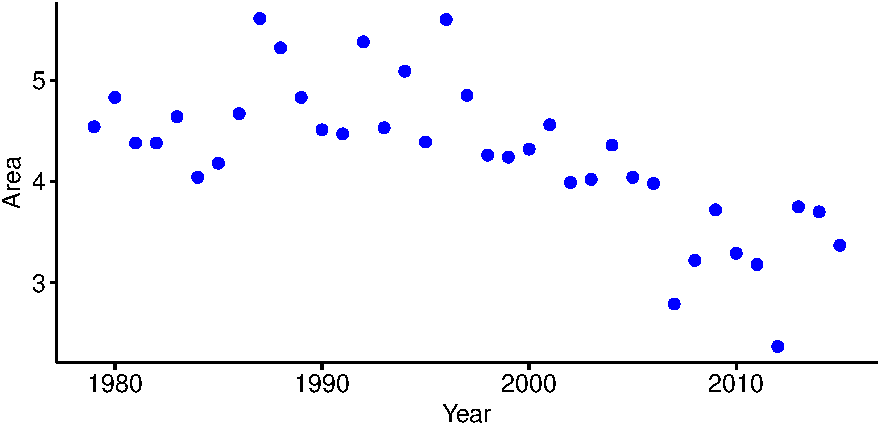
\includegraphics{compbio4all-book_files/figure-latex/unnamed-chunk-94-1.pdf}

Not how R doesn't need extra space for the years where there are no data

\hypertarget{try-it-yourself}{%
\section{Try it yourself}\label{try-it-yourself}}

The original lynx data that comes with R spans the year 1821--1934. Make a sequence of numbers called year.lynx using the \texttt{seq()} command.

\begin{Shaded}
\begin{Highlighting}[]
\DecValTok{1957}\SpecialCharTok{:}\DecValTok{1964}
\end{Highlighting}
\end{Shaded}

\begin{verbatim}
## [1] 1957 1958 1959 1960 1961 1962 1963 1964
\end{verbatim}

There was a hypothesis that sunspot number and/or size impact lynx populations. R has a dataset called sunspots that runs from 1749 to 1983. Make a vector called year year.sunspot using the \texttt{seq()} command.

\begin{Shaded}
\begin{Highlighting}[]
\DecValTok{1749}\SpecialCharTok{:}\DecValTok{1983}
\end{Highlighting}
\end{Shaded}

\begin{verbatim}
##   [1] 1749 1750 1751 1752 1753 1754 1755 1756 1757 1758 1759 1760 1761 1762 1763
##  [16] 1764 1765 1766 1767 1768 1769 1770 1771 1772 1773 1774 1775 1776 1777 1778
##  [31] 1779 1780 1781 1782 1783 1784 1785 1786 1787 1788 1789 1790 1791 1792 1793
##  [46] 1794 1795 1796 1797 1798 1799 1800 1801 1802 1803 1804 1805 1806 1807 1808
##  [61] 1809 1810 1811 1812 1813 1814 1815 1816 1817 1818 1819 1820 1821 1822 1823
##  [76] 1824 1825 1826 1827 1828 1829 1830 1831 1832 1833 1834 1835 1836 1837 1838
##  [91] 1839 1840 1841 1842 1843 1844 1845 1846 1847 1848 1849 1850 1851 1852 1853
## [106] 1854 1855 1856 1857 1858 1859 1860 1861 1862 1863 1864 1865 1866 1867 1868
## [121] 1869 1870 1871 1872 1873 1874 1875 1876 1877 1878 1879 1880 1881 1882 1883
## [136] 1884 1885 1886 1887 1888 1889 1890 1891 1892 1893 1894 1895 1896 1897 1898
## [151] 1899 1900 1901 1902 1903 1904 1905 1906 1907 1908 1909 1910 1911 1912 1913
## [166] 1914 1915 1916 1917 1918 1919 1920 1921 1922 1923 1924 1925 1926 1927 1928
## [181] 1929 1930 1931 1932 1933 1934 1935 1936 1937 1938 1939 1940 1941 1942 1943
## [196] 1944 1945 1946 1947 1948 1949 1950 1951 1952 1953 1954 1955 1956 1957 1958
## [211] 1959 1960 1961 1962 1963 1964 1965 1966 1967 1968 1969 1970 1971 1972 1973
## [226] 1974 1975 1976 1977 1978 1979 1980 1981 1982 1983
\end{verbatim}

\hypertarget{a-complicate-dataframe-to-make}{%
\section{A complicate dataframe to make}\label{a-complicate-dataframe-to-make}}

\hypertarget{build-the-dataframe}{%
\section{Build the dataframe}\label{build-the-dataframe}}

This code makes all of the columns and makes a dataframe

\begin{Shaded}
\begin{Highlighting}[]
\NormalTok{aa        }\OtherTok{\textless{}{-}}\FunctionTok{c}\NormalTok{(}\StringTok{\textquotesingle{}A\textquotesingle{}}\NormalTok{,}\StringTok{\textquotesingle{}C\textquotesingle{}}\NormalTok{,}\StringTok{\textquotesingle{}D\textquotesingle{}}\NormalTok{,}\StringTok{\textquotesingle{}E\textquotesingle{}}\NormalTok{,}\StringTok{\textquotesingle{}F\textquotesingle{}}\NormalTok{,}\StringTok{\textquotesingle{}G\textquotesingle{}}\NormalTok{,}\StringTok{\textquotesingle{}H\textquotesingle{}}\NormalTok{,}\StringTok{\textquotesingle{}I\textquotesingle{}}\NormalTok{,}\StringTok{\textquotesingle{}K\textquotesingle{}}\NormalTok{,}\StringTok{\textquotesingle{}L\textquotesingle{}}\NormalTok{,}\StringTok{\textquotesingle{}M\textquotesingle{}}\NormalTok{,}\StringTok{\textquotesingle{}N\textquotesingle{}}\NormalTok{,}\StringTok{\textquotesingle{}P\textquotesingle{}}\NormalTok{,}\StringTok{\textquotesingle{}Q\textquotesingle{}}\NormalTok{,}\StringTok{\textquotesingle{}R\textquotesingle{}}\NormalTok{,}\StringTok{\textquotesingle{}S\textquotesingle{}}\NormalTok{,}\StringTok{\textquotesingle{}T\textquotesingle{}}\NormalTok{,}\StringTok{\textquotesingle{}V\textquotesingle{}}\NormalTok{,}\StringTok{\textquotesingle{}W\textquotesingle{}}\NormalTok{,}\StringTok{\textquotesingle{}Y\textquotesingle{}}\NormalTok{)}
\NormalTok{MW.da     }\OtherTok{\textless{}{-}}\FunctionTok{c}\NormalTok{(}\DecValTok{89}\NormalTok{,}\DecValTok{121}\NormalTok{,}\DecValTok{133}\NormalTok{,}\DecValTok{146}\NormalTok{,}\DecValTok{165}\NormalTok{,}\DecValTok{75}\NormalTok{,}\DecValTok{155}\NormalTok{,}\DecValTok{131}\NormalTok{,}\DecValTok{146}\NormalTok{,}\DecValTok{131}\NormalTok{,}\DecValTok{149}\NormalTok{,}\DecValTok{132}\NormalTok{,}\DecValTok{115}\NormalTok{,}\DecValTok{147}\NormalTok{,}\DecValTok{174}\NormalTok{,}\DecValTok{105}\NormalTok{,}\DecValTok{119}\NormalTok{,}\DecValTok{117}\NormalTok{,}\DecValTok{204}\NormalTok{,}\DecValTok{181}\NormalTok{)}
\NormalTok{volume    }\OtherTok{\textless{}{-}}\FunctionTok{c}\NormalTok{(}\DecValTok{67}\NormalTok{,}\DecValTok{86}\NormalTok{,}\DecValTok{91}\NormalTok{,}\DecValTok{109}\NormalTok{,}\DecValTok{135}\NormalTok{,}\DecValTok{48}\NormalTok{,}\DecValTok{118}\NormalTok{,}\DecValTok{124}\NormalTok{,}\DecValTok{135}\NormalTok{,}\DecValTok{124}\NormalTok{,}\DecValTok{124}\NormalTok{,}\DecValTok{96}\NormalTok{,}\DecValTok{90}\NormalTok{,}
              \DecValTok{114}\NormalTok{,}\DecValTok{148}\NormalTok{,}\DecValTok{73}\NormalTok{,}\DecValTok{93}\NormalTok{,}\DecValTok{105}\NormalTok{,}\DecValTok{163}\NormalTok{,}\DecValTok{141}\NormalTok{)}
\NormalTok{bulkiness }\OtherTok{\textless{}{-}}\FunctionTok{c}\NormalTok{(}\FloatTok{11.5}\NormalTok{,}\FloatTok{13.46}\NormalTok{,}\FloatTok{11.68}\NormalTok{,}\FloatTok{13.57}\NormalTok{,}\FloatTok{19.8}\NormalTok{,}\FloatTok{3.4}\NormalTok{,}\FloatTok{13.69}\NormalTok{,}\FloatTok{21.4}\NormalTok{,}
              \FloatTok{15.71}\NormalTok{,}\FloatTok{21.4}\NormalTok{,}\FloatTok{16.25}\NormalTok{,}\FloatTok{12.28}\NormalTok{,}\FloatTok{17.43}\NormalTok{,}
              \FloatTok{14.45}\NormalTok{,}\FloatTok{14.28}\NormalTok{,}\FloatTok{9.47}\NormalTok{,}\FloatTok{15.77}\NormalTok{,}\FloatTok{21.57}\NormalTok{,}\FloatTok{21.67}\NormalTok{,}\FloatTok{18.03}\NormalTok{)}
\NormalTok{polarity  }\OtherTok{\textless{}{-}}\FunctionTok{c}\NormalTok{(}\DecValTok{0}\NormalTok{,}\FloatTok{1.48}\NormalTok{,}\FloatTok{49.7}\NormalTok{,}\FloatTok{49.9}\NormalTok{,}\FloatTok{0.35}\NormalTok{,}\DecValTok{0}\NormalTok{,}\FloatTok{51.6}\NormalTok{,}\FloatTok{0.13}\NormalTok{,}\FloatTok{49.5}\NormalTok{,}\FloatTok{0.13}\NormalTok{,}
              \FloatTok{1.43}\NormalTok{,}\FloatTok{3.38}\NormalTok{,}\FloatTok{1.58}\NormalTok{,}\FloatTok{3.53}\NormalTok{,}\DecValTok{52}\NormalTok{,}\FloatTok{1.67}\NormalTok{,}\FloatTok{1.66}\NormalTok{,}\FloatTok{0.13}\NormalTok{,}\FloatTok{2.1}\NormalTok{,}\FloatTok{1.61}\NormalTok{)}
\NormalTok{isoelectric.pt }\OtherTok{\textless{}{-}}\FunctionTok{c}\NormalTok{(}\DecValTok{6}\NormalTok{,}\FloatTok{5.07}\NormalTok{,}\FloatTok{2.77}\NormalTok{,}\FloatTok{3.22}\NormalTok{,}\FloatTok{5.48}\NormalTok{,}\FloatTok{5.97}\NormalTok{,}\FloatTok{7.59}\NormalTok{,}\FloatTok{6.02}\NormalTok{,}\FloatTok{9.74}\NormalTok{,}\FloatTok{5.98}\NormalTok{,}
                   \FloatTok{5.74}\NormalTok{,}\FloatTok{5.41}\NormalTok{,}\FloatTok{6.3}\NormalTok{,}\FloatTok{5.65}\NormalTok{,}\FloatTok{10.76}\NormalTok{,}\FloatTok{5.68}\NormalTok{,}\FloatTok{6.16}\NormalTok{,}\FloatTok{5.96}\NormalTok{,}\FloatTok{5.89}\NormalTok{,}\FloatTok{5.66}\NormalTok{)}
\NormalTok{hydrophobe}\FloatTok{.34} \OtherTok{\textless{}{-}}\FunctionTok{c}\NormalTok{(}\FloatTok{1.8}\NormalTok{,}\FloatTok{2.5}\NormalTok{,}\SpecialCharTok{{-}}\FloatTok{3.5}\NormalTok{,}\SpecialCharTok{{-}}\FloatTok{3.5}\NormalTok{,}\FloatTok{2.8}\NormalTok{,}\SpecialCharTok{{-}}\FloatTok{0.4}\NormalTok{,}\SpecialCharTok{{-}}\FloatTok{3.2}\NormalTok{,}\FloatTok{4.5}\NormalTok{,}\SpecialCharTok{{-}}\FloatTok{3.9}\NormalTok{,}\FloatTok{3.8}\NormalTok{,}\FloatTok{1.9}\NormalTok{,}
                  \SpecialCharTok{{-}}\FloatTok{3.5}\NormalTok{,}\SpecialCharTok{{-}}\FloatTok{1.6}\NormalTok{,}\SpecialCharTok{{-}}\FloatTok{3.5}\NormalTok{,}\SpecialCharTok{{-}}\FloatTok{4.5}\NormalTok{,}\SpecialCharTok{{-}}\FloatTok{0.8}\NormalTok{,}\SpecialCharTok{{-}}\FloatTok{0.7}\NormalTok{,}\FloatTok{4.2}\NormalTok{,}\SpecialCharTok{{-}}\FloatTok{0.9}\NormalTok{,}\SpecialCharTok{{-}}\FloatTok{1.3}\NormalTok{)}
\NormalTok{hydrophobe}\FloatTok{.35} \OtherTok{\textless{}{-}}\FunctionTok{c}\NormalTok{(}\FloatTok{1.6}\NormalTok{,}\DecValTok{2}\NormalTok{,}\SpecialCharTok{{-}}\FloatTok{9.2}\NormalTok{,}\SpecialCharTok{{-}}\FloatTok{8.2}\NormalTok{,}\FloatTok{3.7}\NormalTok{,}\DecValTok{1}\NormalTok{,}\SpecialCharTok{{-}}\DecValTok{3}\NormalTok{,}\FloatTok{3.1}\NormalTok{,}\SpecialCharTok{{-}}\FloatTok{8.8}\NormalTok{,}\FloatTok{2.8}\NormalTok{,}\FloatTok{3.4}\NormalTok{,}\SpecialCharTok{{-}}\FloatTok{4.8}\NormalTok{,}
                  \SpecialCharTok{{-}}\FloatTok{0.2}\NormalTok{,}\SpecialCharTok{{-}}\FloatTok{4.1}\NormalTok{,}\SpecialCharTok{{-}}\FloatTok{12.3}\NormalTok{,}\FloatTok{0.6}\NormalTok{,}\FloatTok{1.2}\NormalTok{,}\FloatTok{2.6}\NormalTok{,}\FloatTok{1.9}\NormalTok{,}\SpecialCharTok{{-}}\FloatTok{0.7}\NormalTok{)}
\NormalTok{saaH2O       }\OtherTok{\textless{}{-}}\FunctionTok{c}\NormalTok{(}\DecValTok{113}\NormalTok{,}\DecValTok{140}\NormalTok{,}\DecValTok{151}\NormalTok{,}\DecValTok{183}\NormalTok{,}\DecValTok{218}\NormalTok{,}\DecValTok{85}\NormalTok{,}\DecValTok{194}\NormalTok{,}\DecValTok{182}\NormalTok{,}\DecValTok{211}\NormalTok{,}\DecValTok{180}\NormalTok{,}\DecValTok{204}\NormalTok{,}\DecValTok{158}\NormalTok{,}
                 \DecValTok{143}\NormalTok{,}\DecValTok{189}\NormalTok{,}\DecValTok{241}\NormalTok{,}\DecValTok{122}\NormalTok{,}\DecValTok{146}\NormalTok{,}\DecValTok{160}\NormalTok{,}\DecValTok{259}\NormalTok{,}\DecValTok{229}\NormalTok{)}
\NormalTok{faal.fold    }\OtherTok{\textless{}{-}}\FunctionTok{c}\NormalTok{(}\FloatTok{0.74}\NormalTok{,}\FloatTok{0.91}\NormalTok{,}\FloatTok{0.62}\NormalTok{,}\FloatTok{0.62}\NormalTok{,}\FloatTok{0.88}\NormalTok{,}\FloatTok{0.72}\NormalTok{,}\FloatTok{0.78}\NormalTok{,}\FloatTok{0.88}\NormalTok{,}\FloatTok{0.52}\NormalTok{,}
                 \FloatTok{0.85}\NormalTok{,}\FloatTok{0.85}\NormalTok{,}\FloatTok{0.63}\NormalTok{,}\FloatTok{0.64}\NormalTok{,}\FloatTok{0.62}\NormalTok{,}\FloatTok{0.64}\NormalTok{,}\FloatTok{0.66}\NormalTok{,}\FloatTok{0.7}\NormalTok{,}\FloatTok{0.86}\NormalTok{,}\FloatTok{0.85}\NormalTok{,}\FloatTok{0.76}\NormalTok{)}
\NormalTok{polar.req    }\OtherTok{\textless{}{-}}\FunctionTok{c}\NormalTok{(}\DecValTok{7}\NormalTok{,}\FloatTok{4.8}\NormalTok{,}\DecValTok{13}\NormalTok{,}\FloatTok{12.5}\NormalTok{,}\DecValTok{5}\NormalTok{,}\FloatTok{7.9}\NormalTok{,}\FloatTok{8.4}\NormalTok{,}\FloatTok{4.9}\NormalTok{,}\FloatTok{10.1}\NormalTok{,}\FloatTok{4.9}\NormalTok{,}\FloatTok{5.3}\NormalTok{,}\DecValTok{10}\NormalTok{,}
                 \FloatTok{6.6}\NormalTok{,}\FloatTok{8.6}\NormalTok{,}\FloatTok{9.1}\NormalTok{,}\FloatTok{7.5}\NormalTok{,}\FloatTok{6.6}\NormalTok{,}\FloatTok{5.6}\NormalTok{,}\FloatTok{5.2}\NormalTok{,}\FloatTok{5.4}\NormalTok{)}
\NormalTok{freq        }\OtherTok{\textless{}{-}}\FunctionTok{c}\NormalTok{(}\FloatTok{7.8}\NormalTok{,}\FloatTok{1.1}\NormalTok{,}\FloatTok{5.19}\NormalTok{,}\FloatTok{6.72}\NormalTok{,}\FloatTok{4.39}\NormalTok{,}\FloatTok{6.77}\NormalTok{,}\FloatTok{2.03}\NormalTok{,}\FloatTok{6.95}\NormalTok{,}\FloatTok{6.32}\NormalTok{,}
                \FloatTok{10.15}\NormalTok{,}\FloatTok{2.28}\NormalTok{,}\FloatTok{4.37}\NormalTok{,}\FloatTok{4.26}\NormalTok{,}\FloatTok{3.45}\NormalTok{,}\FloatTok{5.23}\NormalTok{,}\FloatTok{6.46}\NormalTok{,}\FloatTok{5.12}\NormalTok{,}\FloatTok{7.01}\NormalTok{,}\FloatTok{1.09}\NormalTok{,}\FloatTok{3.3}\NormalTok{)}
\NormalTok{charge}\OtherTok{\textless{}{-}}\FunctionTok{c}\NormalTok{(}\StringTok{\textquotesingle{}un\textquotesingle{}}\NormalTok{,}\StringTok{\textquotesingle{}un\textquotesingle{}}\NormalTok{,}\StringTok{\textquotesingle{}neg\textquotesingle{}}\NormalTok{,}\StringTok{\textquotesingle{}neg\textquotesingle{}}\NormalTok{,}\StringTok{\textquotesingle{}un\textquotesingle{}}\NormalTok{,}\StringTok{\textquotesingle{}un\textquotesingle{}}\NormalTok{,}\StringTok{\textquotesingle{}pos\textquotesingle{}}\NormalTok{,}\StringTok{\textquotesingle{}un\textquotesingle{}}\NormalTok{,}\StringTok{\textquotesingle{}pos\textquotesingle{}}\NormalTok{,}
          \StringTok{\textquotesingle{}un\textquotesingle{}}\NormalTok{,}\StringTok{\textquotesingle{}un\textquotesingle{}}\NormalTok{,}\StringTok{\textquotesingle{}un\textquotesingle{}}\NormalTok{,}\StringTok{\textquotesingle{}un\textquotesingle{}}\NormalTok{,}\StringTok{\textquotesingle{}un\textquotesingle{}}\NormalTok{,}\StringTok{\textquotesingle{}pos\textquotesingle{}}\NormalTok{,}\StringTok{\textquotesingle{}un\textquotesingle{}}\NormalTok{,}\StringTok{\textquotesingle{}un\textquotesingle{}}\NormalTok{,}\StringTok{\textquotesingle{}un\textquotesingle{}}\NormalTok{,}\StringTok{\textquotesingle{}un\textquotesingle{}}\NormalTok{,}\StringTok{\textquotesingle{}un\textquotesingle{}}\NormalTok{)}
\NormalTok{hydropathy}\OtherTok{\textless{}{-}}\FunctionTok{c}\NormalTok{(}\StringTok{\textquotesingle{}hydrophobic\textquotesingle{}}\NormalTok{,}\StringTok{\textquotesingle{}hydrophobic\textquotesingle{}}\NormalTok{,}\StringTok{\textquotesingle{}hydrophilic\textquotesingle{}}\NormalTok{,}\StringTok{\textquotesingle{}}
\StringTok{              hydrophilic\textquotesingle{}}\NormalTok{,}\StringTok{\textquotesingle{}hydrophobic\textquotesingle{}}\NormalTok{,}\StringTok{\textquotesingle{}neutral\textquotesingle{}}\NormalTok{,}\StringTok{\textquotesingle{}neutral\textquotesingle{}}\NormalTok{,}\StringTok{\textquotesingle{}hydrophobic\textquotesingle{}}\NormalTok{,}\StringTok{\textquotesingle{}hydrophilic\textquotesingle{}}\NormalTok{,}\StringTok{\textquotesingle{}hydrophobic\textquotesingle{}}\NormalTok{,}\StringTok{\textquotesingle{}hydrophobic\textquotesingle{}}\NormalTok{,}\StringTok{\textquotesingle{}hydrophilic\textquotesingle{}}\NormalTok{,}\StringTok{\textquotesingle{}neutral\textquotesingle{}}\NormalTok{,}
              \StringTok{\textquotesingle{}hydrophilic\textquotesingle{}}\NormalTok{,}\StringTok{\textquotesingle{}hydrophilic\textquotesingle{}}\NormalTok{,}\StringTok{\textquotesingle{}neutral\textquotesingle{}}\NormalTok{,}\StringTok{\textquotesingle{}neutral\textquotesingle{}}\NormalTok{,}
              \StringTok{\textquotesingle{}hydrophobic\textquotesingle{}}\NormalTok{,}\StringTok{\textquotesingle{}hydrophobic\textquotesingle{}}\NormalTok{,}\StringTok{\textquotesingle{}neutral\textquotesingle{}}\NormalTok{)}
\NormalTok{volume.cat}\OtherTok{\textless{}{-}}\FunctionTok{c}\NormalTok{(}\StringTok{\textquotesingle{}verysmall\textquotesingle{}}\NormalTok{,}\StringTok{\textquotesingle{}small\textquotesingle{}}\NormalTok{,}\StringTok{\textquotesingle{}small\textquotesingle{}}\NormalTok{,}\StringTok{\textquotesingle{}medium\textquotesingle{}}\NormalTok{,}
              \StringTok{\textquotesingle{}verylarge\textquotesingle{}}\NormalTok{,}\StringTok{\textquotesingle{}verysmall\textquotesingle{}}\NormalTok{,}\StringTok{\textquotesingle{}medium\textquotesingle{}}\NormalTok{,}\StringTok{\textquotesingle{}large\textquotesingle{}}\NormalTok{,}\StringTok{\textquotesingle{}large\textquotesingle{}}\NormalTok{,}
              \StringTok{\textquotesingle{}large\textquotesingle{}}\NormalTok{,}\StringTok{\textquotesingle{}large\textquotesingle{}}\NormalTok{,}\StringTok{\textquotesingle{}small\textquotesingle{}}\NormalTok{,}\StringTok{\textquotesingle{}small\textquotesingle{}}\NormalTok{,}\StringTok{\textquotesingle{}medium\textquotesingle{}}\NormalTok{,}\StringTok{\textquotesingle{}large\textquotesingle{}}\NormalTok{,}\StringTok{\textquotesingle{}verysmall\textquotesingle{}}\NormalTok{,}\StringTok{\textquotesingle{}small\textquotesingle{}}\NormalTok{,}\StringTok{\textquotesingle{}medium\textquotesingle{}}\NormalTok{,}\StringTok{\textquotesingle{}verylarge\textquotesingle{}}\NormalTok{,}\StringTok{\textquotesingle{}verylarge\textquotesingle{}}\NormalTok{)}
\NormalTok{polarity.cat}\OtherTok{\textless{}{-}}\FunctionTok{c}\NormalTok{(}\StringTok{\textquotesingle{}nonpolar\textquotesingle{}}\NormalTok{,}\StringTok{\textquotesingle{}nonpolar\textquotesingle{}}\NormalTok{,}\StringTok{\textquotesingle{}polar\textquotesingle{}}\NormalTok{,}\StringTok{\textquotesingle{}polar\textquotesingle{}}\NormalTok{,}
                \StringTok{\textquotesingle{}nonpolar\textquotesingle{}}\NormalTok{,}\StringTok{\textquotesingle{}nonpolar\textquotesingle{}}\NormalTok{,}\StringTok{\textquotesingle{}polar\textquotesingle{}}\NormalTok{,}\StringTok{\textquotesingle{}nonpolar\textquotesingle{}}\NormalTok{,}
                \StringTok{\textquotesingle{}polar\textquotesingle{}}\NormalTok{,}\StringTok{\textquotesingle{}nonpolar\textquotesingle{}}\NormalTok{,}\StringTok{\textquotesingle{}nonpolar\textquotesingle{}}\NormalTok{,}\StringTok{\textquotesingle{}polar\textquotesingle{}}\NormalTok{,}\StringTok{\textquotesingle{}nonpolar\textquotesingle{}}\NormalTok{,}\StringTok{\textquotesingle{}polar\textquotesingle{}}\NormalTok{,}
                \StringTok{\textquotesingle{}polar\textquotesingle{}}\NormalTok{,}\StringTok{\textquotesingle{}polar\textquotesingle{}}\NormalTok{,}\StringTok{\textquotesingle{}polar\textquotesingle{}}\NormalTok{,}\StringTok{\textquotesingle{}nonpolar\textquotesingle{}}\NormalTok{,}\StringTok{\textquotesingle{}nonpolar\textquotesingle{}}\NormalTok{,}\StringTok{\textquotesingle{}polar\textquotesingle{}}\NormalTok{)}
\NormalTok{chemical}\OtherTok{\textless{}{-}}\FunctionTok{c}\NormalTok{(}\StringTok{\textquotesingle{}aliphatic\textquotesingle{}}\NormalTok{,}\StringTok{\textquotesingle{}sulfur\textquotesingle{}}\NormalTok{,}\StringTok{\textquotesingle{}acidic\textquotesingle{}}\NormalTok{,}\StringTok{\textquotesingle{}acidic\textquotesingle{}}\NormalTok{,}\StringTok{\textquotesingle{}aromatic\textquotesingle{}}\NormalTok{,}
            \StringTok{\textquotesingle{}aliphatic\textquotesingle{}}\NormalTok{,}\StringTok{\textquotesingle{}basic\textquotesingle{}}\NormalTok{,}\StringTok{\textquotesingle{}aliphatic\textquotesingle{}}\NormalTok{,}\StringTok{\textquotesingle{}basic\textquotesingle{}}\NormalTok{,}\StringTok{\textquotesingle{}aliphatic\textquotesingle{}}\NormalTok{,}\StringTok{\textquotesingle{}sulfur\textquotesingle{}}\NormalTok{,}
            \StringTok{\textquotesingle{}amide\textquotesingle{}}\NormalTok{,}\StringTok{\textquotesingle{}aliphatic\textquotesingle{}}\NormalTok{,}\StringTok{\textquotesingle{}amide\textquotesingle{}}\NormalTok{,}\StringTok{\textquotesingle{}basic\textquotesingle{}}\NormalTok{,}\StringTok{\textquotesingle{}hydroxyl\textquotesingle{}}\NormalTok{,}\StringTok{\textquotesingle{}hydroxyl\textquotesingle{}}\NormalTok{,}
            \StringTok{\textquotesingle{}aliphatic\textquotesingle{}}\NormalTok{,}\StringTok{\textquotesingle{}aromatic\textquotesingle{}}\NormalTok{,}\StringTok{\textquotesingle{}aromatic\textquotesingle{}}\NormalTok{)}

\NormalTok{aa\_dat }\OtherTok{\textless{}{-}} \FunctionTok{data.frame}\NormalTok{(aa,MW.da,volume,bulkiness,}
\NormalTok{polarity,isoelectric.pt,hydrophobe}\FloatTok{.34}\NormalTok{,hydrophobe}\FloatTok{.35}\NormalTok{,}
\NormalTok{saaH2O,faal.fold, polar.req,freq,charge,hydropathy,volume.cat,polarity.cat,chemical)}
\end{Highlighting}
\end{Shaded}

\hypertarget{references}{%
\section{References}\label{references}}

Poole, Kim G. 2003. A review of the Canada Lynx, \emph{Lynx canadensis} ,in Canada. Canadian {[}Field-Naturalist 117: 360-376.{[}(\url{https://www.canadianfieldnaturalist.ca/index.php/cfn/article/view/738}){]} DOI: \url{https://doi.org/10.22621/cfn.v117i3.738}

\hypertarget{build-your-own-dataframe}{%
\chapter{Build your own dataframe}\label{build-your-own-dataframe}}

\begin{Shaded}
\begin{Highlighting}[]
\NormalTok{lynx.ca }\OtherTok{\textless{}{-}} \FunctionTok{c}\NormalTok{(}\DecValTok{13445}\NormalTok{, }\DecValTok{8625}\NormalTok{, }\DecValTok{6853}\NormalTok{, }\DecValTok{6953}\NormalTok{, }\DecValTok{6574}\NormalTok{,}
  \DecValTok{8265}\NormalTok{, }\DecValTok{9977}\NormalTok{, }\DecValTok{7579}\NormalTok{, }\DecValTok{11542}\NormalTok{, }\DecValTok{7180}\NormalTok{,}
  \DecValTok{4713}\NormalTok{, }\DecValTok{4907}\NormalTok{, }\DecValTok{2819}\NormalTok{, }\DecValTok{5171}\NormalTok{, }\DecValTok{6873}\NormalTok{, }
  \DecValTok{6148}\NormalTok{, }\DecValTok{8573}\NormalTok{, }\DecValTok{9361}\NormalTok{, }\DecValTok{11226}\NormalTok{)}
\end{Highlighting}
\end{Shaded}

\begin{Shaded}
\begin{Highlighting}[]
\NormalTok{year }\OtherTok{\textless{}{-}} \FunctionTok{c}\NormalTok{(}\DecValTok{1984}\NormalTok{, }\DecValTok{1985}\NormalTok{, }\DecValTok{1986}\NormalTok{, }\DecValTok{1987}\NormalTok{,}
          \DecValTok{1988}\NormalTok{, }\DecValTok{1989}\NormalTok{, }\DecValTok{1990}\NormalTok{, }\DecValTok{1991}\NormalTok{, }\DecValTok{1992}\NormalTok{, }
          \DecValTok{1993}\NormalTok{, }\DecValTok{1994}\NormalTok{, }\DecValTok{1995}\NormalTok{, }\DecValTok{1996}\NormalTok{, }\DecValTok{1997}\NormalTok{,}
          \DecValTok{1998}\NormalTok{, }\DecValTok{1999}\NormalTok{, }\DecValTok{2000}\NormalTok{, }\DecValTok{2001}\NormalTok{, }\DecValTok{2002}\NormalTok{)}
\end{Highlighting}
\end{Shaded}

\begin{Shaded}
\begin{Highlighting}[]
\NormalTok{lynx.new }\OtherTok{\textless{}{-}} \FunctionTok{data.frame}\NormalTok{(}\AttributeTok{lynx.ca =}\NormalTok{ lynx.ca,}
                       \AttributeTok{year =}\NormalTok{ year)}
\end{Highlighting}
\end{Shaded}

\begin{Shaded}
\begin{Highlighting}[]
\FunctionTok{plot}\NormalTok{(lynx.ca }\SpecialCharTok{\textasciitilde{}}\NormalTok{ year, }\AttributeTok{data =}\NormalTok{ lynx.new)}
\end{Highlighting}
\end{Shaded}

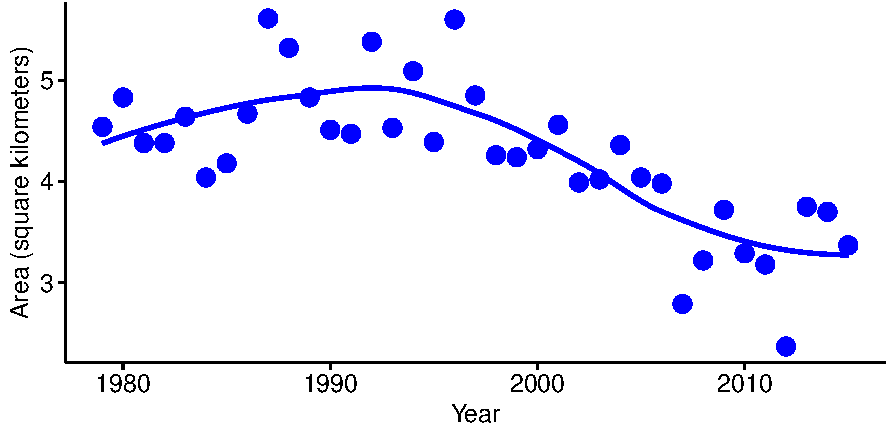
\includegraphics{compbio4all-book_files/figure-latex/unnamed-chunk-101-1.pdf}

As in the lynx dataset that comes with R, we see wild swings in abundance over short periods of time.

\hypertarget{your-turn-1}{%
\section{Your turn}\label{your-turn-1}}

Make this plot pretty

\hypertarget{references-1}{%
\section{References}\label{references-1}}

Poole, Kim G. 2003. A review of the Canada Lynx, \emph{Lynx canadensis} ,in Canada. Canadian {[}Field-Naturalist 117: 360-376.{[}(\url{https://www.canadianfieldnaturalist.ca/index.php/cfn/article/view/738}){]} DOI: \url{https://doi.org/10.22621/cfn.v117i3.738}

\hypertarget{build-your-own-dataframe-1}{%
\chapter{Build your own dataframe}\label{build-your-own-dataframe-1}}

\begin{Shaded}
\begin{Highlighting}[]
\NormalTok{lynx.ca }\OtherTok{\textless{}{-}} \FunctionTok{c}\NormalTok{(}\DecValTok{13445}\NormalTok{, }\DecValTok{8625}\NormalTok{, }\DecValTok{6853}\NormalTok{, }\DecValTok{6953}\NormalTok{, }\DecValTok{6574}\NormalTok{,}
  \DecValTok{8265}\NormalTok{, }\DecValTok{9977}\NormalTok{, }\DecValTok{7579}\NormalTok{, }\DecValTok{11542}\NormalTok{, }\DecValTok{7180}\NormalTok{,}
  \DecValTok{4713}\NormalTok{, }\DecValTok{4907}\NormalTok{, }\DecValTok{2819}\NormalTok{, }\DecValTok{5171}\NormalTok{, }\DecValTok{6873}\NormalTok{, }
  \DecValTok{6148}\NormalTok{, }\DecValTok{8573}\NormalTok{, }\DecValTok{9361}\NormalTok{, }\DecValTok{11226}\NormalTok{)}
\end{Highlighting}
\end{Shaded}

\begin{Shaded}
\begin{Highlighting}[]
\NormalTok{year }\OtherTok{\textless{}{-}} \FunctionTok{c}\NormalTok{(}\DecValTok{1984}\NormalTok{, }\DecValTok{1985}\NormalTok{, }\DecValTok{1986}\NormalTok{, }\DecValTok{1987}\NormalTok{,}
          \DecValTok{1988}\NormalTok{, }\DecValTok{1989}\NormalTok{, }\DecValTok{1990}\NormalTok{, }\DecValTok{1991}\NormalTok{, }\DecValTok{1992}\NormalTok{, }
          \DecValTok{1993}\NormalTok{, }\DecValTok{1994}\NormalTok{, }\DecValTok{1995}\NormalTok{, }\DecValTok{1996}\NormalTok{, }\DecValTok{1997}\NormalTok{,}
          \DecValTok{1998}\NormalTok{, }\DecValTok{1999}\NormalTok{, }\DecValTok{2000}\NormalTok{, }\DecValTok{2001}\NormalTok{, }\DecValTok{2002}\NormalTok{)}
\end{Highlighting}
\end{Shaded}

\begin{Shaded}
\begin{Highlighting}[]
\NormalTok{lynx.new }\OtherTok{\textless{}{-}} \FunctionTok{data.frame}\NormalTok{(}\AttributeTok{lynx.ca =}\NormalTok{ lynx.ca,}
                       \AttributeTok{year =}\NormalTok{ year)}
\end{Highlighting}
\end{Shaded}

\begin{Shaded}
\begin{Highlighting}[]
\FunctionTok{plot}\NormalTok{(lynx.ca }\SpecialCharTok{\textasciitilde{}}\NormalTok{ year, }\AttributeTok{data =}\NormalTok{ lynx.new)}
\end{Highlighting}
\end{Shaded}

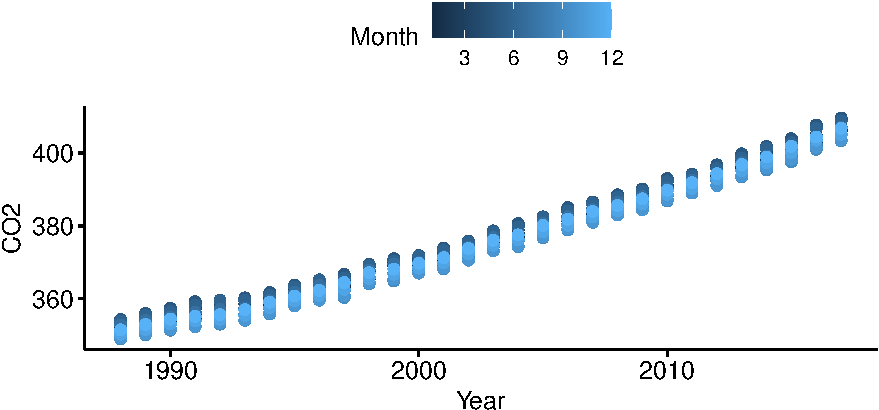
\includegraphics{compbio4all-book_files/figure-latex/unnamed-chunk-105-1.pdf}

As in the lynx dataset that comes with R, we see wild swings in abundance over short periods of time.

\hypertarget{your-turn-2}{%
\section{Your turn}\label{your-turn-2}}

Make this plot pretty

\hypertarget{references-2}{%
\section{References}\label{references-2}}

Poole, Kim G. 2003. A review of the Canada Lynx, \emph{Lynx canadensis} ,in Canada. Canadian {[}Field-Naturalist 117: 360-376.{[}(\url{https://www.canadianfieldnaturalist.ca/index.php/cfn/article/view/738}){]} DOI: \url{https://doi.org/10.22621/cfn.v117i3.738}

\hypertarget{introduction-to-ggplot-and-ggpubr}{%
\chapter{Introduction to ggplot and ggpubr}\label{introduction-to-ggplot-and-ggpubr}}

\#\#SeaIce

\begin{Shaded}
\begin{Highlighting}[]
\FunctionTok{library}\NormalTok{(Stat2Data)}
\FunctionTok{library}\NormalTok{(ggplot2)}
\FunctionTok{library}\NormalTok{(ggpubr)}
\end{Highlighting}
\end{Shaded}

\begin{Shaded}
\begin{Highlighting}[]
\FunctionTok{data}\NormalTok{(SeaIce)}
\end{Highlighting}
\end{Shaded}

\begin{Shaded}
\begin{Highlighting}[]
\FunctionTok{ggscatter}\NormalTok{(}\AttributeTok{y =} \StringTok{"Area"}\NormalTok{,}
          \AttributeTok{x =} \StringTok{"Year"}\NormalTok{,}
          \AttributeTok{data =}\NormalTok{ SeaIce)}
\end{Highlighting}
\end{Shaded}

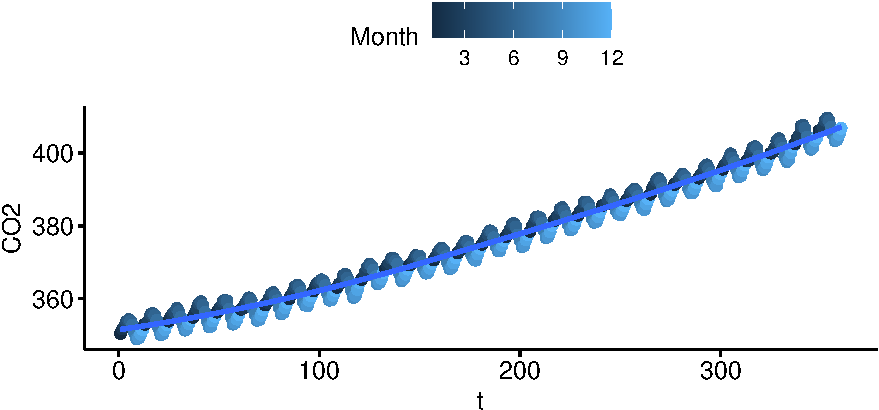
\includegraphics{compbio4all-book_files/figure-latex/unnamed-chunk-108-1.pdf}

\begin{Shaded}
\begin{Highlighting}[]
\FunctionTok{ggscatter}\NormalTok{(}\AttributeTok{y =} \StringTok{"Area"}\NormalTok{,}
          \AttributeTok{x =} \StringTok{"Year"}\NormalTok{,}
          \AttributeTok{color =} \StringTok{"blue"}\NormalTok{, }\CommentTok{\#in quotes}
          \AttributeTok{data =}\NormalTok{ SeaIce)}
\end{Highlighting}
\end{Shaded}

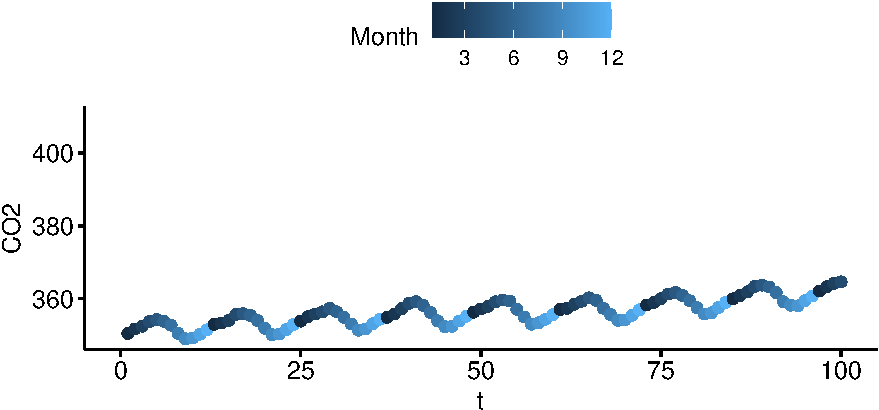
\includegraphics{compbio4all-book_files/figure-latex/unnamed-chunk-109-1.pdf}

\begin{Shaded}
\begin{Highlighting}[]
\FunctionTok{ggscatter}\NormalTok{(}\AttributeTok{y =} \StringTok{"Area"}\NormalTok{,}
          \AttributeTok{x =} \StringTok{"Year"}\NormalTok{,}
          \AttributeTok{color =} \StringTok{"blue"}\NormalTok{,}
          \AttributeTok{shape =} \DecValTok{16}\NormalTok{,     }\CommentTok{\# not quotes}
          \AttributeTok{data =}\NormalTok{ SeaIce)}
\end{Highlighting}
\end{Shaded}

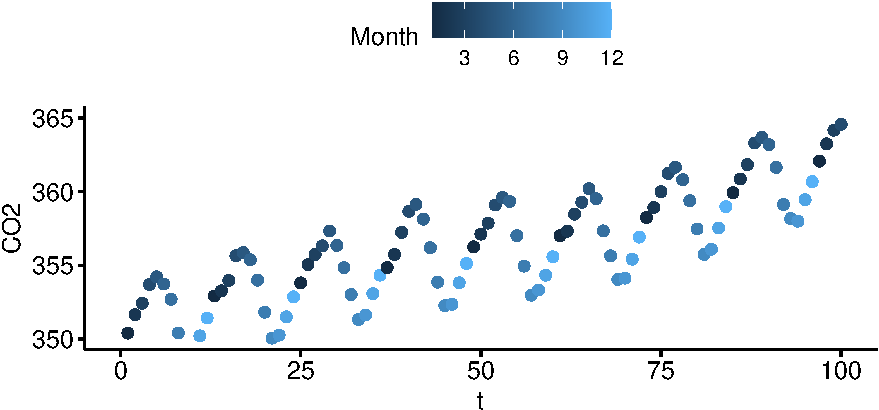
\includegraphics{compbio4all-book_files/figure-latex/unnamed-chunk-110-1.pdf}

\begin{Shaded}
\begin{Highlighting}[]
\FunctionTok{ggscatter}\NormalTok{(}\AttributeTok{y =} \StringTok{"Area"}\NormalTok{,}
          \AttributeTok{x =} \StringTok{"Year"}\NormalTok{,}
          \AttributeTok{color =} \StringTok{"blue"}\NormalTok{,}
          \AttributeTok{shape =} \DecValTok{16}\NormalTok{,     }\CommentTok{\# }
          \AttributeTok{size =} \DecValTok{4}\NormalTok{,       }\CommentTok{\# not quotes}
          \AttributeTok{data =}\NormalTok{ SeaIce)}
\end{Highlighting}
\end{Shaded}

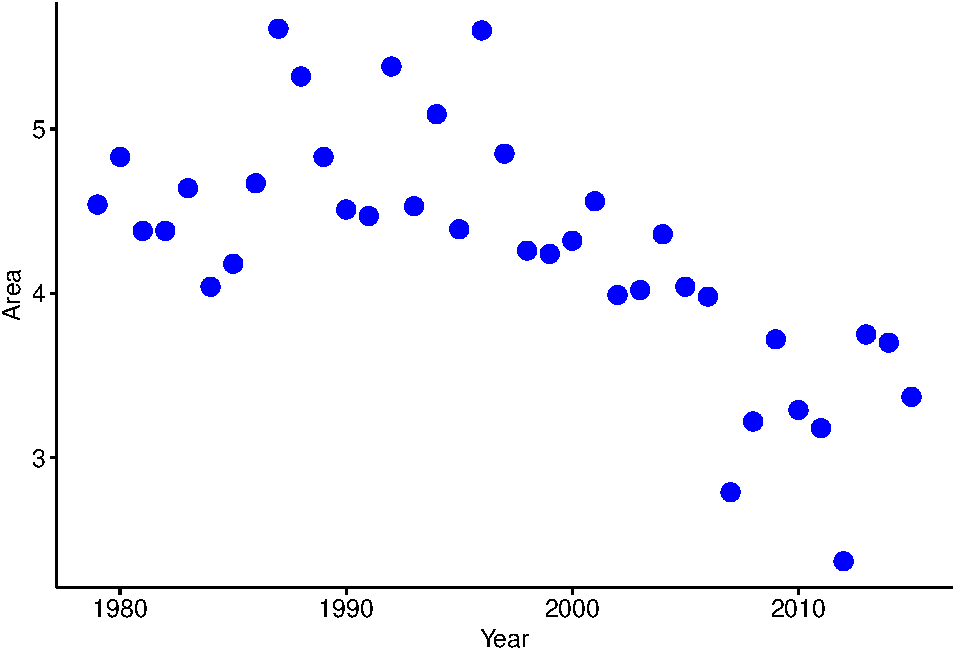
\includegraphics{compbio4all-book_files/figure-latex/unnamed-chunk-111-1.pdf}

\begin{Shaded}
\begin{Highlighting}[]
\FunctionTok{ggscatter}\NormalTok{(}\AttributeTok{y =} \StringTok{"Area"}\NormalTok{,}
          \AttributeTok{x =} \StringTok{"Year"}\NormalTok{,}
          \AttributeTok{color =} \StringTok{"blue"}\NormalTok{,}
          \AttributeTok{shape =} \DecValTok{16}\NormalTok{,     }\CommentTok{\# }
          \AttributeTok{size =} \DecValTok{4}\NormalTok{,       }\CommentTok{\# }
          \AttributeTok{ylab =} \StringTok{"Area (square kilometers)"}\NormalTok{, }\CommentTok{\# in quotes}
          \AttributeTok{data =}\NormalTok{ SeaIce)}
\end{Highlighting}
\end{Shaded}

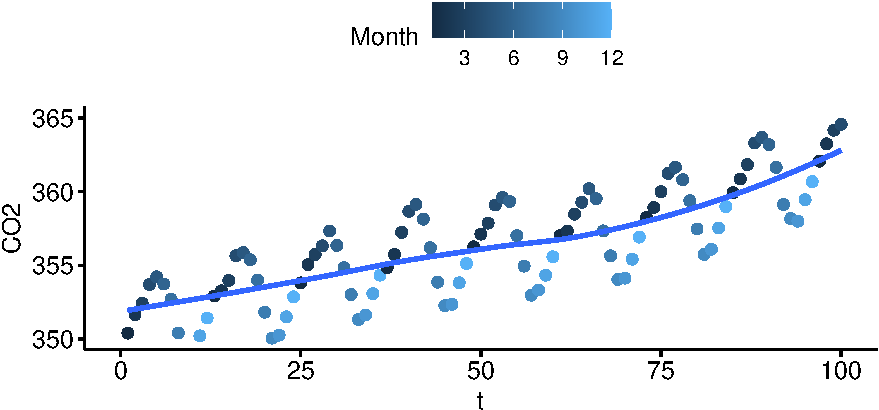
\includegraphics{compbio4all-book_files/figure-latex/unnamed-chunk-112-1.pdf}

\hypertarget{regression-line}{%
\section{Regression line}\label{regression-line}}

\begin{Shaded}
\begin{Highlighting}[]
\FunctionTok{ggscatter}\NormalTok{(}\AttributeTok{y =} \StringTok{"Area"}\NormalTok{,}
          \AttributeTok{x =} \StringTok{"Year"}\NormalTok{,}
          \AttributeTok{color =} \StringTok{"blue"}\NormalTok{,}
          \AttributeTok{shape =} \DecValTok{16}\NormalTok{,     }\CommentTok{\# }
          \AttributeTok{size =} \DecValTok{4}\NormalTok{,       }\CommentTok{\# }
          \AttributeTok{ylab =} \StringTok{"Area (square kilometers)"}\NormalTok{, }
          \AttributeTok{add =} \StringTok{"reg.line"}\NormalTok{,}
          \AttributeTok{data =}\NormalTok{ SeaIce)}
\end{Highlighting}
\end{Shaded}

\begin{verbatim}
## `geom_smooth()` using formula 'y ~ x'
\end{verbatim}

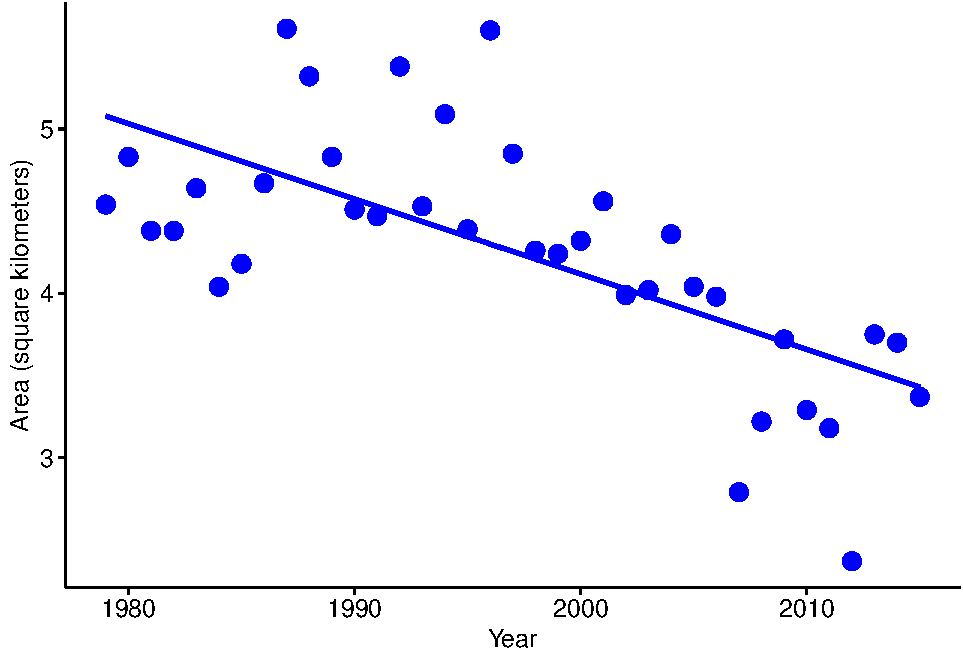
\includegraphics{compbio4all-book_files/figure-latex/unnamed-chunk-113-1.pdf}

\begin{Shaded}
\begin{Highlighting}[]
\FunctionTok{ggscatter}\NormalTok{(}\AttributeTok{y =} \StringTok{"Area"}\NormalTok{,}
          \AttributeTok{x =} \StringTok{"Year"}\NormalTok{,}
          \AttributeTok{color =} \StringTok{"blue"}\NormalTok{,}
          \AttributeTok{shape =} \DecValTok{16}\NormalTok{,     }\CommentTok{\# }
          \AttributeTok{size =} \DecValTok{4}\NormalTok{,       }\CommentTok{\# }
          \AttributeTok{ylab =} \StringTok{"Area (square kilometers)"}\NormalTok{, }
          \AttributeTok{add =} \StringTok{"reg.line"}\NormalTok{,}
          \AttributeTok{data =}\NormalTok{ SeaIce) }\SpecialCharTok{+}
  \FunctionTok{stat\_regline\_equation}\NormalTok{()}
\end{Highlighting}
\end{Shaded}

\begin{verbatim}
## `geom_smooth()` using formula 'y ~ x'
\end{verbatim}

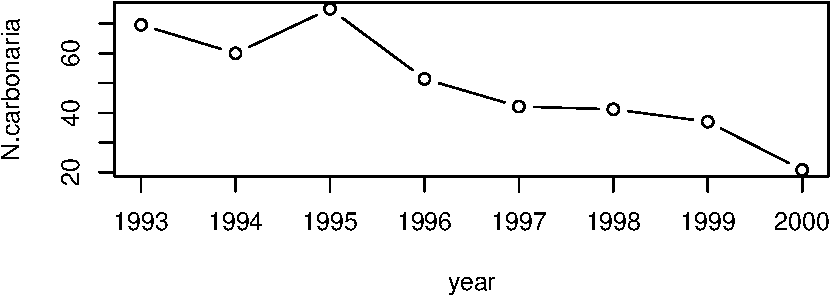
\includegraphics{compbio4all-book_files/figure-latex/unnamed-chunk-114-1.pdf}

Why is equation different

\begin{Shaded}
\begin{Highlighting}[]
\FunctionTok{ggscatter}\NormalTok{(}\AttributeTok{y =} \StringTok{"Area"}\NormalTok{,}
          \AttributeTok{x =} \StringTok{"t"}\NormalTok{,}
          \AttributeTok{color =} \StringTok{"blue"}\NormalTok{,}
          \AttributeTok{shape =} \DecValTok{16}\NormalTok{,     }\CommentTok{\# }
          \AttributeTok{size =} \DecValTok{4}\NormalTok{,       }\CommentTok{\# }
          \AttributeTok{ylab =} \StringTok{"Area (square kilometers)"}\NormalTok{, }
          \AttributeTok{add =} \StringTok{"reg.line"}\NormalTok{,}
          \AttributeTok{data =}\NormalTok{ SeaIce) }\SpecialCharTok{+}
  \FunctionTok{stat\_regline\_equation}\NormalTok{()}
\end{Highlighting}
\end{Shaded}

\begin{verbatim}
## `geom_smooth()` using formula 'y ~ x'
\end{verbatim}

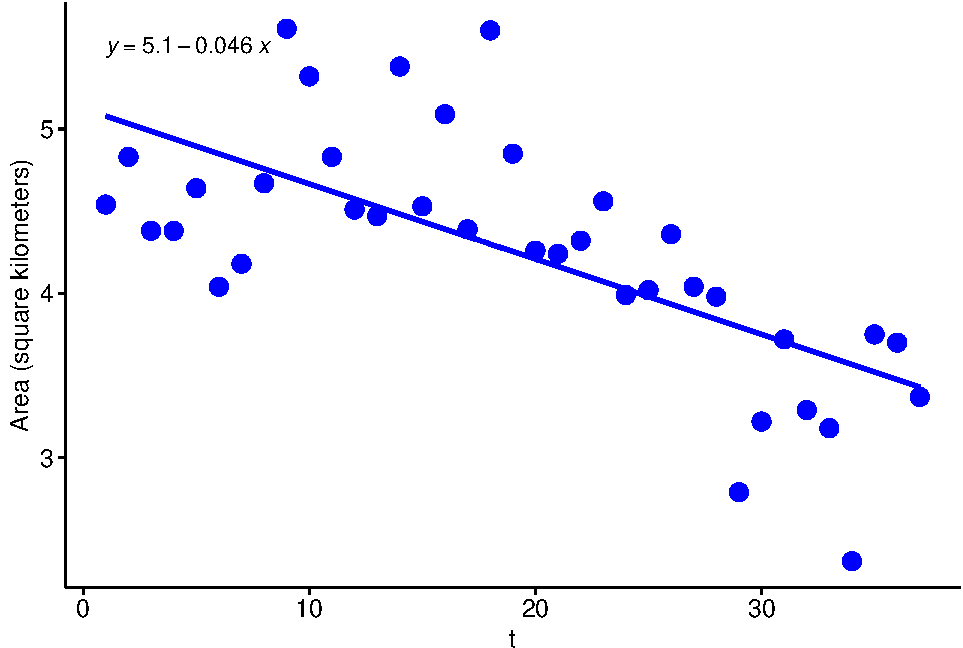
\includegraphics{compbio4all-book_files/figure-latex/unnamed-chunk-115-1.pdf}

\hypertarget{smoother}{%
\section{Smoother}\label{smoother}}

\begin{Shaded}
\begin{Highlighting}[]
\FunctionTok{ggscatter}\NormalTok{(}\AttributeTok{y =} \StringTok{"Area"}\NormalTok{,}
          \AttributeTok{x =} \StringTok{"Year"}\NormalTok{,}
          \AttributeTok{color =} \StringTok{"blue"}\NormalTok{,}
          \AttributeTok{shape =} \DecValTok{16}\NormalTok{,     }\CommentTok{\# }
          \AttributeTok{size =} \DecValTok{4}\NormalTok{,       }\CommentTok{\# }
          \AttributeTok{ylab =} \StringTok{"Area (square kilometers)"}\NormalTok{, }
          \AttributeTok{add =} \StringTok{"loess"}\NormalTok{,}
          \AttributeTok{data =}\NormalTok{ SeaIce)}
\end{Highlighting}
\end{Shaded}

\begin{verbatim}
## `geom_smooth()` using formula 'y ~ x'
\end{verbatim}

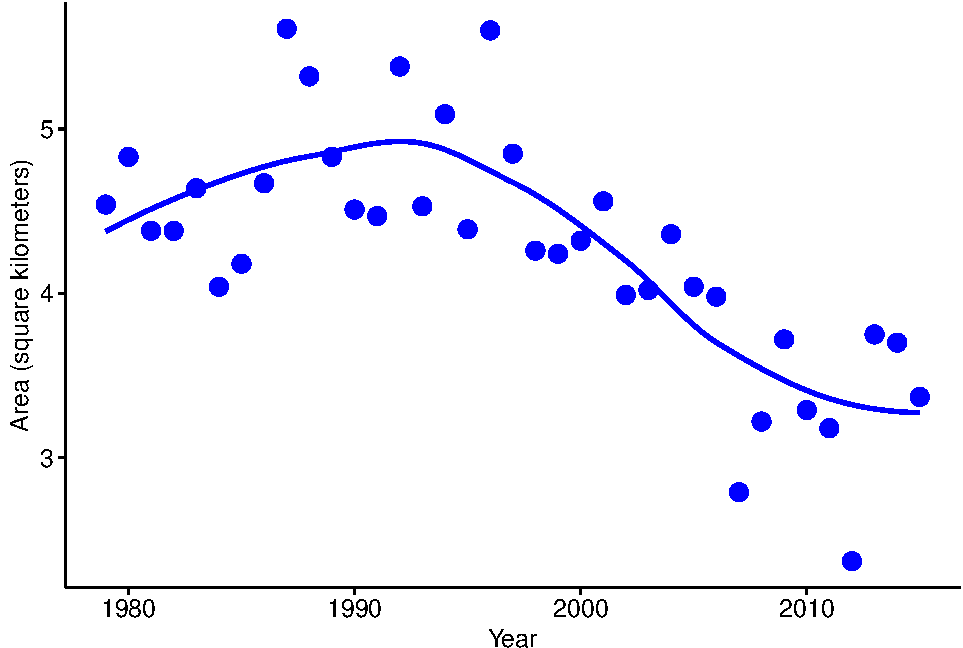
\includegraphics{compbio4all-book_files/figure-latex/unnamed-chunk-116-1.pdf}

\hypertarget{correlation}{%
\section{correlation}\label{correlation}}

\begin{Shaded}
\begin{Highlighting}[]
\FunctionTok{ggscatter}\NormalTok{(}\AttributeTok{y =} \StringTok{"Area"}\NormalTok{,}
          \AttributeTok{x =} \StringTok{"Year"}\NormalTok{,}
          \AttributeTok{color =} \StringTok{"blue"}\NormalTok{,}
          \AttributeTok{shape =} \DecValTok{16}\NormalTok{,     }\CommentTok{\# }
          \AttributeTok{size =} \DecValTok{4}\NormalTok{,       }\CommentTok{\# }
          \AttributeTok{ylab =} \StringTok{"Area (square kilometers)"}\NormalTok{,  }
          \AttributeTok{cor.coef =}\NormalTok{ T,}
          \AttributeTok{data =}\NormalTok{ SeaIce)}
\end{Highlighting}
\end{Shaded}

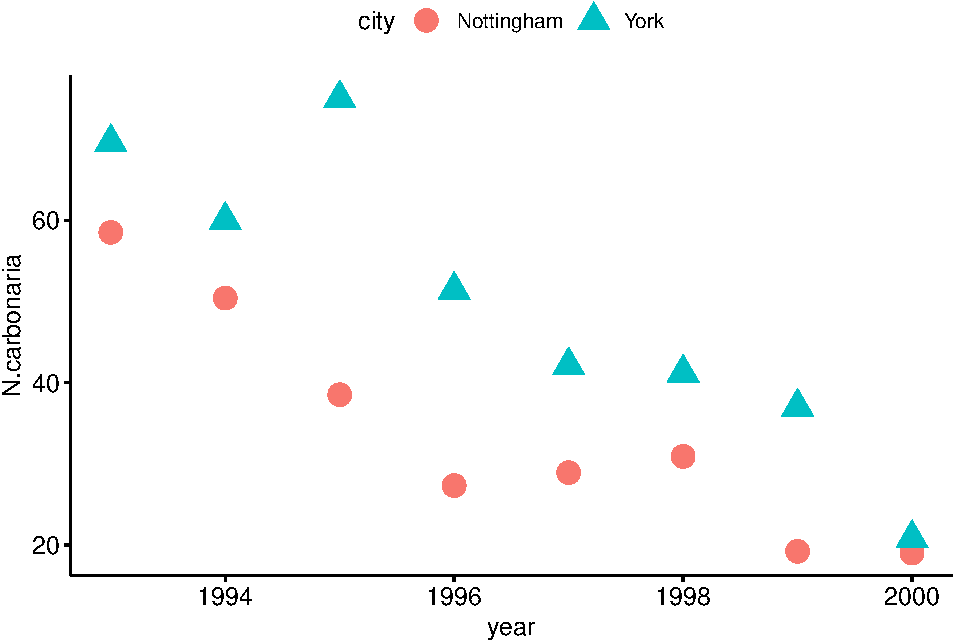
\includegraphics{compbio4all-book_files/figure-latex/unnamed-chunk-117-1.pdf}

\hypertarget{long-time-series}{%
\section{Long time series}\label{long-time-series}}

\begin{Shaded}
\begin{Highlighting}[]
\FunctionTok{data}\NormalTok{(CO2Hawaii)}
\end{Highlighting}
\end{Shaded}

Year

Why stacked?

\begin{Shaded}
\begin{Highlighting}[]
\FunctionTok{ggscatter}\NormalTok{(}\AttributeTok{y =} \StringTok{"CO2"}\NormalTok{,}
       \AttributeTok{x =} \StringTok{"Year"}\NormalTok{,}
       \AttributeTok{data =}\NormalTok{ CO2Hawaii)}
\end{Highlighting}
\end{Shaded}

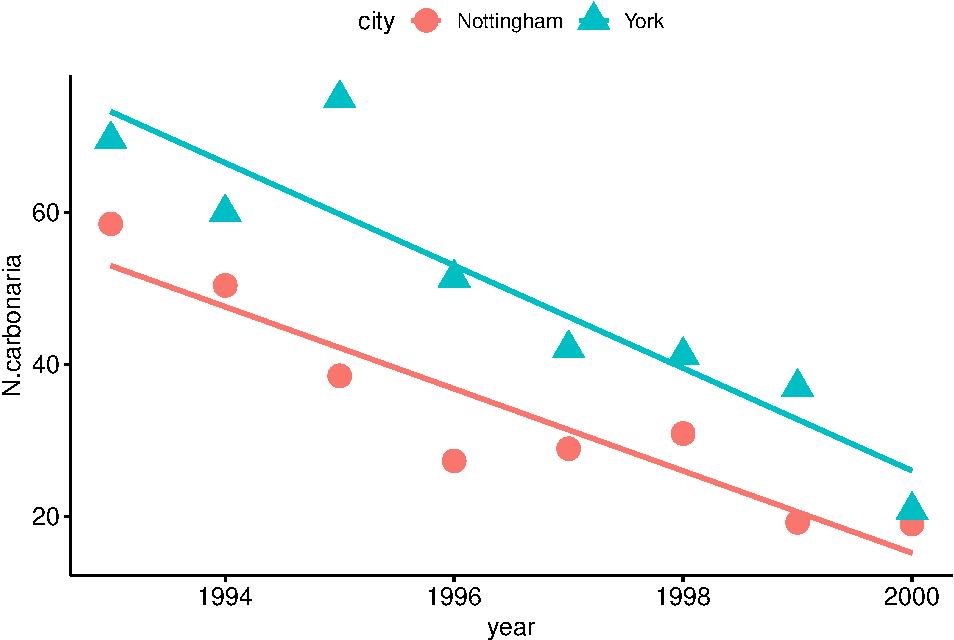
\includegraphics{compbio4all-book_files/figure-latex/unnamed-chunk-119-1.pdf}

\begin{Shaded}
\begin{Highlighting}[]
\FunctionTok{ggscatter}\NormalTok{(}\AttributeTok{y =} \StringTok{"CO2"}\NormalTok{,}
       \AttributeTok{x =} \StringTok{"Year"}\NormalTok{,}
       \AttributeTok{color =} \StringTok{"Month"}\NormalTok{,}
       \AttributeTok{data =}\NormalTok{ CO2Hawaii)}
\end{Highlighting}
\end{Shaded}

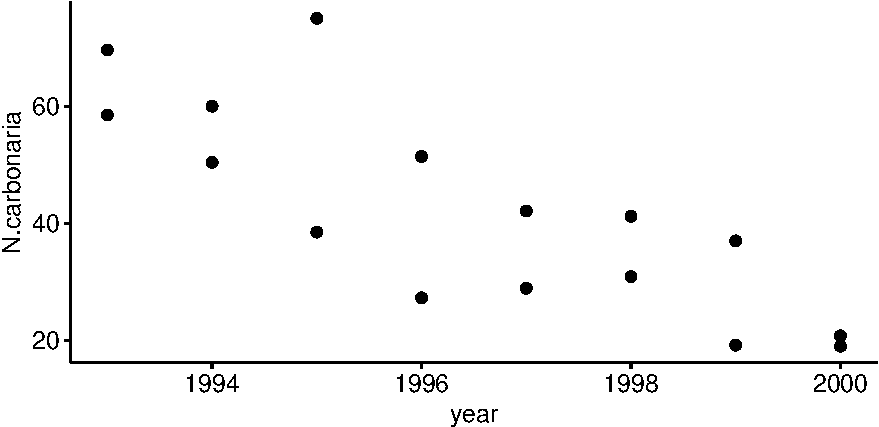
\includegraphics{compbio4all-book_files/figure-latex/unnamed-chunk-120-1.pdf}

What's different?

\begin{Shaded}
\begin{Highlighting}[]
\FunctionTok{ggscatter}\NormalTok{(}\AttributeTok{y =} \StringTok{"CO2"}\NormalTok{,}
       \AttributeTok{x =} \StringTok{"t"}\NormalTok{,}
       \AttributeTok{color =} \StringTok{"Month"}\NormalTok{,}
       \AttributeTok{data =}\NormalTok{ CO2Hawaii)}
\end{Highlighting}
\end{Shaded}

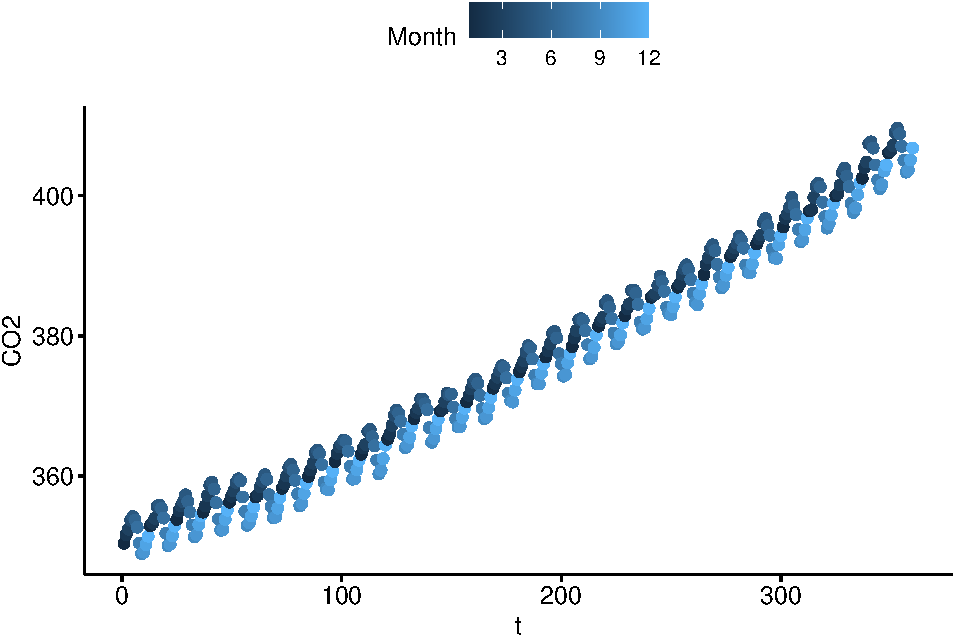
\includegraphics{compbio4all-book_files/figure-latex/unnamed-chunk-121-1.pdf}

\begin{Shaded}
\begin{Highlighting}[]
\FunctionTok{ggscatter}\NormalTok{(}\AttributeTok{y =} \StringTok{"CO2"}\NormalTok{,}
       \AttributeTok{x =} \StringTok{"t"}\NormalTok{,}
       \AttributeTok{color =} \StringTok{"Month"}\NormalTok{,}
       \AttributeTok{add =} \StringTok{"reg.line"}\NormalTok{,}
       \AttributeTok{data =}\NormalTok{ CO2Hawaii)}
\end{Highlighting}
\end{Shaded}

\begin{verbatim}
## `geom_smooth()` using formula 'y ~ x'
\end{verbatim}

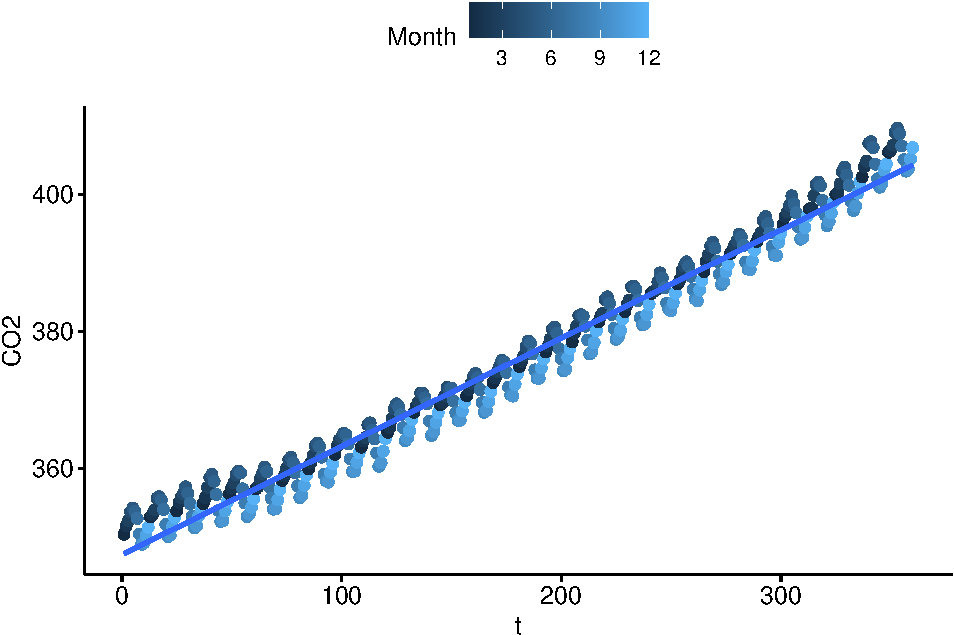
\includegraphics{compbio4all-book_files/figure-latex/unnamed-chunk-122-1.pdf}

\begin{Shaded}
\begin{Highlighting}[]
\FunctionTok{ggscatter}\NormalTok{(}\AttributeTok{y =} \StringTok{"CO2"}\NormalTok{,}
       \AttributeTok{x =} \StringTok{"t"}\NormalTok{,}
       \AttributeTok{color =} \StringTok{"Month"}\NormalTok{,}
       \AttributeTok{add =} \StringTok{"loess"}\NormalTok{,}
       \AttributeTok{data =}\NormalTok{ CO2Hawaii)}
\end{Highlighting}
\end{Shaded}

\begin{verbatim}
## `geom_smooth()` using formula 'y ~ x'
\end{verbatim}

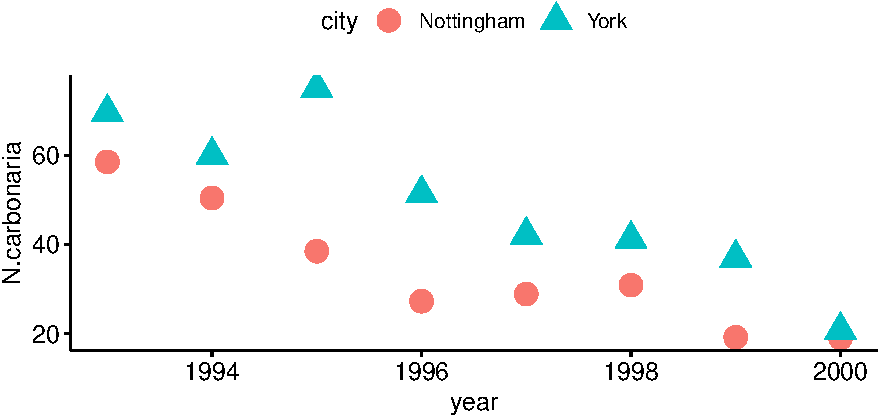
\includegraphics{compbio4all-book_files/figure-latex/unnamed-chunk-123-1.pdf}

\begin{verbatim}


```r
ggscatter(y = "CO2",
       x = "t",
       color = "Month",
       data = CO2Hawaii) +
  xlim(0,100)
\end{verbatim}

\begin{verbatim}
## Warning: Removed 260 rows containing missing values (geom_point).
\end{verbatim}

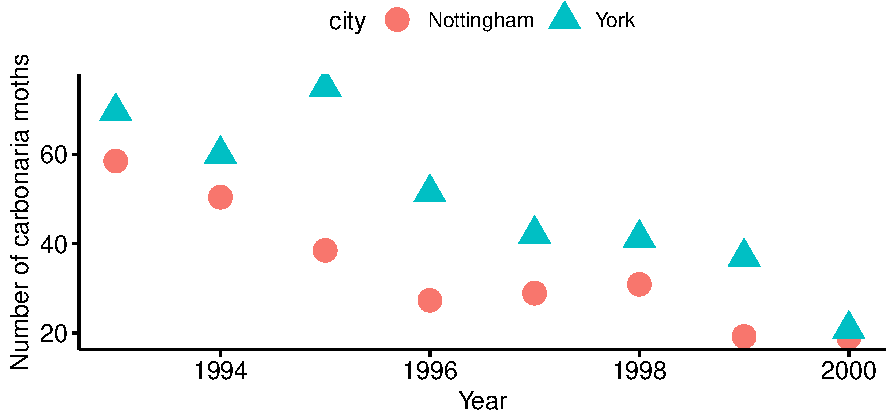
\includegraphics{compbio4all-book_files/figure-latex/unnamed-chunk-124-1.pdf}

\begin{Shaded}
\begin{Highlighting}[]
\FunctionTok{ggscatter}\NormalTok{(}\AttributeTok{y =} \StringTok{"CO2"}\NormalTok{,}
       \AttributeTok{x =} \StringTok{"t"}\NormalTok{,}
       \AttributeTok{color =} \StringTok{"Month"}\NormalTok{,}
       \AttributeTok{data =}\NormalTok{ CO2Hawaii) }\SpecialCharTok{+}
  \FunctionTok{xlim}\NormalTok{(}\DecValTok{0}\NormalTok{,}\DecValTok{100}\NormalTok{) }\SpecialCharTok{+}
  \FunctionTok{ylim}\NormalTok{(}\DecValTok{350}\NormalTok{,}\DecValTok{365}\NormalTok{)}
\end{Highlighting}
\end{Shaded}

\begin{verbatim}
## Warning: Removed 262 rows containing missing values (geom_point).
\end{verbatim}

\includegraphics{compbio4all-book_files/figure-latex/unnamed-chunk-125-1.pdf}

\begin{Shaded}
\begin{Highlighting}[]
\FunctionTok{ggscatter}\NormalTok{(}\AttributeTok{y =} \StringTok{"CO2"}\NormalTok{,}
       \AttributeTok{x =} \StringTok{"t"}\NormalTok{,}
       \AttributeTok{color =} \StringTok{"Month"}\NormalTok{,}
       \AttributeTok{add =} \StringTok{"reg.line"}\NormalTok{,}
       \AttributeTok{data =}\NormalTok{ CO2Hawaii) }\SpecialCharTok{+}
  \FunctionTok{xlim}\NormalTok{(}\DecValTok{0}\NormalTok{,}\DecValTok{100}\NormalTok{) }\SpecialCharTok{+}
  \FunctionTok{ylim}\NormalTok{(}\DecValTok{350}\NormalTok{,}\DecValTok{365}\NormalTok{)}
\end{Highlighting}
\end{Shaded}

\begin{verbatim}
## `geom_smooth()` using formula 'y ~ x'
\end{verbatim}

\begin{verbatim}
## Warning: Removed 262 rows containing non-finite values (stat_smooth).
\end{verbatim}

\begin{verbatim}
## Warning: Removed 262 rows containing missing values (geom_point).
\end{verbatim}

\includegraphics{compbio4all-book_files/figure-latex/unnamed-chunk-126-1.pdf}

\begin{Shaded}
\begin{Highlighting}[]
\FunctionTok{ggscatter}\NormalTok{(}\AttributeTok{y =} \StringTok{"CO2"}\NormalTok{,}
       \AttributeTok{x =} \StringTok{"t"}\NormalTok{,}
       \AttributeTok{color =} \StringTok{"Month"}\NormalTok{,}
       \AttributeTok{add =} \StringTok{"loess"}\NormalTok{,}
       \AttributeTok{data =}\NormalTok{ CO2Hawaii) }\SpecialCharTok{+}
  \FunctionTok{xlim}\NormalTok{(}\DecValTok{0}\NormalTok{,}\DecValTok{100}\NormalTok{) }\SpecialCharTok{+}
  \FunctionTok{ylim}\NormalTok{(}\DecValTok{350}\NormalTok{,}\DecValTok{365}\NormalTok{)}
\end{Highlighting}
\end{Shaded}

\begin{verbatim}
## `geom_smooth()` using formula 'y ~ x'
\end{verbatim}

\begin{verbatim}
## Warning: Removed 262 rows containing non-finite values (stat_smooth).
\end{verbatim}

\begin{verbatim}
## Warning: Removed 262 rows containing missing values (geom_point).
\end{verbatim}

\includegraphics{compbio4all-book_files/figure-latex/unnamed-chunk-127-1.pdf}

\#\#Moth data - 2 cities

Cook and Grant 2000. Frequency of insularia during the decline
in melanics in the peppered. Heredity 85: 580-585.

Make dataframe

\#\#Nottingham data

\begin{Shaded}
\begin{Highlighting}[]
\NormalTok{year.nottingham }\OtherTok{\textless{}{-}} \FunctionTok{seq}\NormalTok{(}\AttributeTok{from =} \DecValTok{1993}\NormalTok{,}
                       \AttributeTok{to =} \DecValTok{2000}\NormalTok{)}
\NormalTok{carbonaria.nottingham }\OtherTok{\textless{}{-}} \FunctionTok{c}\NormalTok{(}\FloatTok{58.5}\NormalTok{, }\FloatTok{50.4}\NormalTok{, }\FloatTok{38.5}\NormalTok{, }\FloatTok{27.3}\NormalTok{, }\FloatTok{28.9}\NormalTok{, }
                           \FloatTok{30.9}\NormalTok{, }\FloatTok{19.2}\NormalTok{, }\DecValTok{19}\NormalTok{)}

\NormalTok{df.nottingham }\OtherTok{\textless{}{-}} \FunctionTok{data.frame}\NormalTok{(}\AttributeTok{year =}\NormalTok{ year.nottingham,}
                            \AttributeTok{N.carbonaria =}\NormalTok{ carbonaria.nottingham,}
                            \AttributeTok{city =} \StringTok{"Nottingham"}\NormalTok{)}

\FunctionTok{plot}\NormalTok{(N.carbonaria }\SpecialCharTok{\textasciitilde{}}\NormalTok{ year, }\AttributeTok{data =}\NormalTok{  df.nottingham, }\AttributeTok{type =} \StringTok{"b"}\NormalTok{)}
\end{Highlighting}
\end{Shaded}

\includegraphics{compbio4all-book_files/figure-latex/unnamed-chunk-128-1.pdf}

How many times did R print ``Nottingham'' How did it make that choice?

\begin{Shaded}
\begin{Highlighting}[]
\NormalTok{year.york }\OtherTok{\textless{}{-}} \FunctionTok{seq}\NormalTok{(}\AttributeTok{from =} \DecValTok{1993}\NormalTok{,}
                 \AttributeTok{to =} \DecValTok{2000}\NormalTok{)}

\NormalTok{carbonaria.york }\OtherTok{\textless{}{-}} \FunctionTok{c}\NormalTok{( }\FloatTok{69.6}\NormalTok{, }\DecValTok{60}\NormalTok{, }\FloatTok{75.0}\NormalTok{, }\FloatTok{51.4}\NormalTok{, }\FloatTok{42.1}\NormalTok{,}
                      \FloatTok{41.2}\NormalTok{, }\FloatTok{37.0}\NormalTok{, }\FloatTok{20.8}\NormalTok{)}

\NormalTok{df.york }\OtherTok{\textless{}{-}} \FunctionTok{data.frame}\NormalTok{(}\AttributeTok{year =}\NormalTok{ year.york,}
                      \AttributeTok{N.carbonaria =}\NormalTok{ carbonaria.york,}
                      \AttributeTok{city =} \StringTok{"York"}\NormalTok{)}

\FunctionTok{plot}\NormalTok{(N.carbonaria }\SpecialCharTok{\textasciitilde{}}\NormalTok{ year, }\AttributeTok{data =}\NormalTok{  df.york, }\AttributeTok{type =} \StringTok{"b"}\NormalTok{)}
\end{Highlighting}
\end{Shaded}

\includegraphics{compbio4all-book_files/figure-latex/unnamed-chunk-129-1.pdf}

\begin{Shaded}
\begin{Highlighting}[]
\NormalTok{df.moth }\OtherTok{\textless{}{-}} \FunctionTok{rbind}\NormalTok{(df.nottingham,}
\NormalTok{                 df.york)}
\end{Highlighting}
\end{Shaded}

\begin{Shaded}
\begin{Highlighting}[]
\FunctionTok{is}\NormalTok{(df.moth)}
\end{Highlighting}
\end{Shaded}

\begin{verbatim}
## [1] "data.frame" "list"       "oldClass"   "vector"
\end{verbatim}

\begin{Shaded}
\begin{Highlighting}[]
\FunctionTok{dim}\NormalTok{(df.moth)}
\end{Highlighting}
\end{Shaded}

\begin{verbatim}
## [1] 16  3
\end{verbatim}

\begin{Shaded}
\begin{Highlighting}[]
\CommentTok{\# install.packages("ggplot2")}
\end{Highlighting}
\end{Shaded}

\begin{Shaded}
\begin{Highlighting}[]
\FunctionTok{library}\NormalTok{(ggplot2)}
\FunctionTok{library}\NormalTok{(ggpubr)}
\end{Highlighting}
\end{Shaded}

\begin{Shaded}
\begin{Highlighting}[]
\FunctionTok{ggscatter}\NormalTok{(}\AttributeTok{y =} \StringTok{"N.carbonaria"}\NormalTok{,   }\CommentTok{\# in quotes}
          \AttributeTok{x =} \StringTok{"year"}\NormalTok{,           }\CommentTok{\# in quotes}
          \AttributeTok{data =}\NormalTok{ df.moth)       }\CommentTok{\# in quotes}
\end{Highlighting}
\end{Shaded}

\includegraphics{compbio4all-book_files/figure-latex/unnamed-chunk-135-1.pdf}

\begin{Shaded}
\begin{Highlighting}[]
\FunctionTok{ggscatter}\NormalTok{(}\AttributeTok{y =} \StringTok{"N.carbonaria"}\NormalTok{, }
          \AttributeTok{x =} \StringTok{"year"}\NormalTok{,}
          \AttributeTok{color =} \StringTok{"city"}\NormalTok{,    }\CommentTok{\# in quotes}
          \AttributeTok{data =}\NormalTok{ df.moth)}
\end{Highlighting}
\end{Shaded}

\includegraphics{compbio4all-book_files/figure-latex/unnamed-chunk-136-1.pdf}

\begin{Shaded}
\begin{Highlighting}[]
\FunctionTok{ggscatter}\NormalTok{(}\AttributeTok{y =} \StringTok{"N.carbonaria"}\NormalTok{,}
          \AttributeTok{x =} \StringTok{"year"}\NormalTok{,}
          \AttributeTok{color =} \StringTok{"city"}\NormalTok{,}
          \AttributeTok{shape =} \StringTok{"city"}\NormalTok{,     }\CommentTok{\# in quotes}
          \AttributeTok{data =}\NormalTok{ df.moth)}
\end{Highlighting}
\end{Shaded}

\includegraphics{compbio4all-book_files/figure-latex/unnamed-chunk-137-1.pdf}

\begin{Shaded}
\begin{Highlighting}[]
\FunctionTok{ggscatter}\NormalTok{(}\AttributeTok{y =} \StringTok{"N.carbonaria"}\NormalTok{,}
          \AttributeTok{x =} \StringTok{"year"}\NormalTok{,}
          \AttributeTok{color =} \StringTok{"city"}\NormalTok{,}
          \AttributeTok{shape =} \StringTok{"city"}\NormalTok{,}
          \AttributeTok{size =} \DecValTok{5}\NormalTok{,       }\CommentTok{\# not in quotes!}
          \AttributeTok{data =}\NormalTok{ df.moth)}
\end{Highlighting}
\end{Shaded}

\includegraphics{compbio4all-book_files/figure-latex/unnamed-chunk-138-1.pdf}

\begin{Shaded}
\begin{Highlighting}[]
\FunctionTok{ggscatter}\NormalTok{(}\AttributeTok{y =} \StringTok{"N.carbonaria"}\NormalTok{,}
          \AttributeTok{x =} \StringTok{"year"}\NormalTok{,}
          \AttributeTok{color =} \StringTok{"city"}\NormalTok{,}
          \AttributeTok{shape =} \StringTok{"city"}\NormalTok{,}
          \AttributeTok{size =} \DecValTok{5}\NormalTok{,       }
          \AttributeTok{data =}\NormalTok{ df.moth,}
          \AttributeTok{ylab =} \StringTok{"Number of carbonaria moths"}\NormalTok{, }\CommentTok{\# labels in quotes}
          \AttributeTok{xlab =} \StringTok{"Year"}\NormalTok{)   }\CommentTok{\# in quotes}
\end{Highlighting}
\end{Shaded}

\includegraphics{compbio4all-book_files/figure-latex/unnamed-chunk-139-1.pdf}

\hypertarget{regression-lines}{%
\section{Regression lines}\label{regression-lines}}

\begin{Shaded}
\begin{Highlighting}[]
\FunctionTok{ggscatter}\NormalTok{(}\AttributeTok{y =} \StringTok{"N.carbonaria"}\NormalTok{,}
          \AttributeTok{x =} \StringTok{"year"}\NormalTok{,}
          \AttributeTok{data =}\NormalTok{ df.moth,}
          \AttributeTok{color =} \StringTok{"city"}\NormalTok{,}
          \AttributeTok{shape =} \StringTok{"city"}\NormalTok{,}
          \AttributeTok{add =} \StringTok{"reg.line"}\NormalTok{,}
          \AttributeTok{size =} \DecValTok{5}\NormalTok{)}
\end{Highlighting}
\end{Shaded}

\begin{verbatim}
## `geom_smooth()` using formula 'y ~ x'
\end{verbatim}

\includegraphics{compbio4all-book_files/figure-latex/unnamed-chunk-140-1.pdf}

\begin{Shaded}
\begin{Highlighting}[]
\FunctionTok{ggscatter}\NormalTok{(}\AttributeTok{y =} \StringTok{"N.carbonaria"}\NormalTok{,}
          \AttributeTok{x =} \StringTok{"year"}\NormalTok{,}
          \AttributeTok{data =}\NormalTok{ df.moth,}
          \AttributeTok{color =} \StringTok{"city"}\NormalTok{,}
          \AttributeTok{shape =} \StringTok{"city"}\NormalTok{,}
          \AttributeTok{add =} \StringTok{"reg.line"}\NormalTok{,}
          \AttributeTok{conf.int =}\NormalTok{ T,}
          \AttributeTok{size =} \DecValTok{5}\NormalTok{)}
\end{Highlighting}
\end{Shaded}

\begin{verbatim}
## `geom_smooth()` using formula 'y ~ x'
\end{verbatim}

\includegraphics{compbio4all-book_files/figure-latex/unnamed-chunk-141-1.pdf}

Only 1 line

\begin{Shaded}
\begin{Highlighting}[]
\FunctionTok{ggscatter}\NormalTok{(}\AttributeTok{y =} \StringTok{"N.carbonaria"}\NormalTok{,}
          \AttributeTok{x =} \StringTok{"year"}\NormalTok{,}
          \AttributeTok{data =}\NormalTok{ df.moth,}
          \AttributeTok{color =} \StringTok{"city"}\NormalTok{,}
          \AttributeTok{shape =} \StringTok{"city"}\NormalTok{,}
          \AttributeTok{add =} \StringTok{"reg.line"}\NormalTok{,}
          \AttributeTok{conf.int =}\NormalTok{ T,}
          \AttributeTok{size =} \DecValTok{5}\NormalTok{) }\SpecialCharTok{+}
  \FunctionTok{stat\_regline\_equation}\NormalTok{()}
\end{Highlighting}
\end{Shaded}

\begin{verbatim}
## `geom_smooth()` using formula 'y ~ x'
\end{verbatim}

\includegraphics{compbio4all-book_files/figure-latex/unnamed-chunk-142-1.pdf}

Facetings - regressions for both lines

\begin{Shaded}
\begin{Highlighting}[]
\FunctionTok{ggscatter}\NormalTok{(}\AttributeTok{y =} \StringTok{"N.carbonaria"}\NormalTok{,}
          \AttributeTok{x =} \StringTok{"year"}\NormalTok{,}
          \AttributeTok{data =}\NormalTok{ df.moth,}
          \AttributeTok{color =} \StringTok{"city"}\NormalTok{,}
          \AttributeTok{shape =} \StringTok{"city"}\NormalTok{,}
          \AttributeTok{add =} \StringTok{"reg.line"}\NormalTok{,}
          \AttributeTok{conf.int =}\NormalTok{ T,}
          \AttributeTok{facet.by =} \StringTok{"city"}\NormalTok{,}
          \AttributeTok{size =} \DecValTok{5}\NormalTok{) }\SpecialCharTok{+}
  \FunctionTok{stat\_regline\_equation}\NormalTok{()}
\end{Highlighting}
\end{Shaded}

\begin{verbatim}
## `geom_smooth()` using formula 'y ~ x'
\end{verbatim}

\includegraphics{compbio4all-book_files/figure-latex/unnamed-chunk-143-1.pdf}

\hypertarget{correlations}{%
\section{Correlations}\label{correlations}}

Only 1 correlations coeffient

\begin{Shaded}
\begin{Highlighting}[]
\FunctionTok{ggscatter}\NormalTok{(}\AttributeTok{y =} \StringTok{"N.carbonaria"}\NormalTok{,}
          \AttributeTok{x =} \StringTok{"year"}\NormalTok{,}
          \AttributeTok{color =} \StringTok{"city"}\NormalTok{,}
          \AttributeTok{shape =} \StringTok{"city"}\NormalTok{,}
          \AttributeTok{size =} \DecValTok{5}\NormalTok{,       }
          \AttributeTok{data =}\NormalTok{ df.moth,}
          \AttributeTok{cor.coef =}\NormalTok{ T,}
          \AttributeTok{ylab =} \StringTok{"Number of carbonaria moths"}\NormalTok{, }\CommentTok{\# labels in quotes}
          \AttributeTok{xlab =} \StringTok{"Year"}\NormalTok{)   }\CommentTok{\# in quotes}
\end{Highlighting}
\end{Shaded}

\includegraphics{compbio4all-book_files/figure-latex/unnamed-chunk-144-1.pdf}

Faceting gives us 2

\begin{Shaded}
\begin{Highlighting}[]
\FunctionTok{ggscatter}\NormalTok{(}\AttributeTok{y =} \StringTok{"N.carbonaria"}\NormalTok{,}
          \AttributeTok{x =} \StringTok{"year"}\NormalTok{,}
          \AttributeTok{color =} \StringTok{"city"}\NormalTok{,}
          \AttributeTok{shape =} \StringTok{"city"}\NormalTok{,}
          \AttributeTok{size =} \DecValTok{5}\NormalTok{,       }
          \AttributeTok{data =}\NormalTok{ df.moth,}
          \AttributeTok{cor.coef =}\NormalTok{ T,}
          \AttributeTok{facet.by =} \StringTok{"city"}\NormalTok{,}
          \AttributeTok{ylab =} \StringTok{"Number of carbonaria moths"}\NormalTok{, }\CommentTok{\# labels in quotes}
          \AttributeTok{xlab =} \StringTok{"Year"}\NormalTok{)   }\CommentTok{\# in quotes}
\end{Highlighting}
\end{Shaded}

\includegraphics{compbio4all-book_files/figure-latex/unnamed-chunk-145-1.pdf}

\begin{Shaded}
\begin{Highlighting}[]
\FunctionTok{ggplot}\NormalTok{(}\AttributeTok{data =}\NormalTok{ df.moth,}
        \FunctionTok{aes}\NormalTok{(}\AttributeTok{y =}\NormalTok{ N.carbonaria,}
            \AttributeTok{x =}\NormalTok{ year,}
            \AttributeTok{color =}\NormalTok{ city)) }\SpecialCharTok{+}
  \FunctionTok{geom\_point}\NormalTok{() }\SpecialCharTok{+}
  \FunctionTok{geom\_line}\NormalTok{()}
\end{Highlighting}
\end{Shaded}

\includegraphics{compbio4all-book_files/figure-latex/unnamed-chunk-146-1.pdf}

\hypertarget{original-data}{%
\section{Original data}\label{original-data}}

\begin{Shaded}
\begin{Highlighting}[]
\CommentTok{\# Cook and Grant 2000.  Frequency of insularia during the decline}
\CommentTok{\# in melanics in the peppered.  Heredity 85: 580{-}585.}
\NormalTok{year.nottingham }\OtherTok{\textless{}{-}} \FunctionTok{seq}\NormalTok{(}\AttributeTok{from =} \DecValTok{1993}\NormalTok{,}
                       \AttributeTok{to =} \DecValTok{2000}\NormalTok{)}
\NormalTok{carbonaria.nottingham }\OtherTok{\textless{}{-}} \FunctionTok{c}\NormalTok{(}\FloatTok{58.5}\NormalTok{, }\FloatTok{50.4}\NormalTok{, }\FloatTok{38.5}\NormalTok{, }\FloatTok{27.3}\NormalTok{, }\FloatTok{28.9}\NormalTok{, }
                           \FloatTok{30.9}\NormalTok{,}\FloatTok{19.2}\NormalTok{, }\DecValTok{19}\NormalTok{)}

\FunctionTok{plot}\NormalTok{(carbonaria.nottingham }\SpecialCharTok{\textasciitilde{}}\NormalTok{ year.nottingham)}
\end{Highlighting}
\end{Shaded}

\includegraphics{compbio4all-book_files/figure-latex/unnamed-chunk-147-1.pdf}

\begin{Shaded}
\begin{Highlighting}[]
\NormalTok{year.york }\OtherTok{\textless{}{-}} \FunctionTok{seq}\NormalTok{(}\AttributeTok{from =} \DecValTok{1990}\NormalTok{,}
                 \AttributeTok{to =} \DecValTok{2000}\NormalTok{)}

\NormalTok{carbonaria.york }\OtherTok{\textless{}{-}} \FunctionTok{c}\NormalTok{(}\FloatTok{57.9}\NormalTok{, }\FloatTok{61.8}\NormalTok{, }\FloatTok{74.1}\NormalTok{, }\FloatTok{69.6}\NormalTok{, }\DecValTok{60}\NormalTok{, }\FloatTok{75.0}\NormalTok{,}
                     \FloatTok{51.4}\NormalTok{, }\FloatTok{42.1}\NormalTok{, }\FloatTok{41.2}\NormalTok{, }\FloatTok{37.0}\NormalTok{, }\FloatTok{20.8}\NormalTok{)}

\FunctionTok{plot}\NormalTok{(carbonaria.york }\SpecialCharTok{\textasciitilde{}}\NormalTok{ year.york)}
\end{Highlighting}
\end{Shaded}

\includegraphics{compbio4all-book_files/figure-latex/unnamed-chunk-147-2.pdf}

\begin{Shaded}
\begin{Highlighting}[]
\NormalTok{year.manchester }\OtherTok{\textless{}{-}} \FunctionTok{c}\NormalTok{(}\StringTok{"1952{-}1964"}\NormalTok{, }\StringTok{"1968{-}1974"}\NormalTok{, }\StringTok{"1990{-}1998"}\NormalTok{)}
\NormalTok{carbonaria.manchester }\OtherTok{\textless{}{-}} \FunctionTok{c}\NormalTok{(}\FloatTok{98.5}\NormalTok{,}\FloatTok{95.9}\NormalTok{,}\FloatTok{20.8}\NormalTok{)}










\NormalTok{year.kent }\OtherTok{\textless{}{-}} \FunctionTok{c}\NormalTok{(}\DecValTok{1971}\NormalTok{, }\DecValTok{1975}\NormalTok{, }\DecValTok{1979}\NormalTok{, }\DecValTok{1983}\NormalTok{, }\DecValTok{1987}\NormalTok{, }
               \DecValTok{1990}\NormalTok{, }\DecValTok{1991}\NormalTok{, }\DecValTok{1992}\NormalTok{, }\DecValTok{1993}\NormalTok{, }\DecValTok{1994}\NormalTok{)}
\NormalTok{carbonaria.kent }\OtherTok{\textless{}{-}} \FunctionTok{c}\NormalTok{(}\FloatTok{78.2}\NormalTok{, }\FloatTok{76.6}\NormalTok{, }\FloatTok{71.7}\NormalTok{, }\FloatTok{64.7}\NormalTok{, }\FloatTok{54.3}\NormalTok{, }
                     \FloatTok{42.3}\NormalTok{, }\FloatTok{30.9}\NormalTok{, }\FloatTok{33.5}\NormalTok{, }\FloatTok{23.0}\NormalTok{, }\FloatTok{23.8}\NormalTok{)}
\FunctionTok{plot}\NormalTok{(carbonaria.kent }\SpecialCharTok{\textasciitilde{}}\NormalTok{ year.kent)}
\end{Highlighting}
\end{Shaded}

\includegraphics{compbio4all-book_files/figure-latex/unnamed-chunk-147-3.pdf}

\begin{Shaded}
\begin{Highlighting}[]
\NormalTok{year.hampshire }\OtherTok{\textless{}{-}} \FunctionTok{c}\NormalTok{(}\StringTok{"1957{-}1964"}\NormalTok{,}\StringTok{"1965{-}1970"}\NormalTok{,}\StringTok{"1973{-}1977"}\NormalTok{)}
\NormalTok{carbonaria.hampshire }\OtherTok{\textless{}{-}} \FunctionTok{c}\NormalTok{(}\FloatTok{7.1}\NormalTok{,}\FloatTok{5.8}\NormalTok{,}\FloatTok{6.5}\NormalTok{)}
\end{Highlighting}
\end{Shaded}

Long time series

insularia, not carboneria!

Clarke, Mani and Wynne. 1985. Evolution in reverse: clean air and the pepperred moth.
Biological Journal of the Linnean Society 26: 189-199.

\hypertarget{loading-packages-data-from-github}{%
\chapter{Loading packages \& data from GitHub}\label{loading-packages-data-from-github}}

TODO= change wildlifeR to compbio4all?

\hypertarget{introduction}{%
\section{Introduction}\label{introduction}}

\textbf{GitHub} is an online platform for hosting and sharing code. More formally it is called a \textbf{software repository}. It is very popular with software developers, especially those creating open-source applications, and has also been adopted whole-hearted by many data scientists and data analysts.

GitHub has many features and uses. One of the most basic ones is to use GitHub like Dropbox to R backup copies of code on GitHub. GitHub also can act like a kind of web server to host websites, online books like this one, and provide access to open source software. Many people working on R packages use GitHub to host their package while its being developed or expanded. When a package is finished, it often is then submitted to CRAN, and the version on GitHub is used as the \textbf{developement version} where new features are being developed and tested.

You can access packages on GitHub to get the newest version before something has been submitted to CRAN, or packages that haven't or maybe will never end up on CRAN. This book relies on a package I've written called \textbf{wildlifeR} for datasets and some functions. In this short exercise we'll download a package from CRAN we need to interact with GitHub, and then download wildlifeR. We'll also go to the wildlifeR website to learn more about the package.

\hypertarget{learning-objectives}{%
\subsection{Learning objectives}\label{learning-objectives}}

\hypertarget{learning-goals}{%
\subsection{Learning goals}\label{learning-goals}}

\hypertarget{functions-arguements-1}{%
\subsection{Functions \& Arguements}\label{functions-arguements-1}}

\begin{itemize}
\tightlist
\item
  library
\item
  devtools::install\_github
\item
  scatter.smooth
\item
  \$
\end{itemize}

\hypertarget{packages}{%
\subsection{Packages}\label{packages}}

\begin{itemize}
\tightlist
\item
  devtools
\item
  wildlifeR
\end{itemize}

\hypertarget{potential-hangups}{%
\subsection{Potential hangups}\label{potential-hangups}}

\begin{itemize}
\tightlist
\item
  We'll use the ``\$'' operator to tell scatter.smooth() what to plot, which is different than how ggpubr and ggplot2 work; sigh\ldots{}
\end{itemize}

\hypertarget{accessing-github-using-devtools}{%
\section{{[} {]} Accessing GitHub using devtools}\label{accessing-github-using-devtools}}

The devtools package is used by many people who write R packages and includes a function for downloading from GitHub

\begin{Shaded}
\begin{Highlighting}[]
\FunctionTok{install.packages}\NormalTok{(}\StringTok{"devtools"}\NormalTok{, }\AttributeTok{dependencies =} \ConstantTok{TRUE}\NormalTok{) }\CommentTok{\# [ ]}
\end{Highlighting}
\end{Shaded}

devtools has a lot of dependencies so this might take a while.

Once everything is downloaded, load the package explicitly with library()

\begin{Shaded}
\begin{Highlighting}[]
\FunctionTok{library}\NormalTok{(devtools)}
\end{Highlighting}
\end{Shaded}

\begin{verbatim}
## Loading required package: usethis
\end{verbatim}

\hypertarget{downloading-the-compbio4all-package-with-install_github}{%
\section{{[} {]} Downloading the compbio4all package with install\_github()}\label{downloading-the-compbio4all-package-with-install_github}}

My github site is at \url{https://github.com/brouwern} and the code for wildlifeR is \url{https://github.com/brouwern/wildlifeR}. You can access the files directly if you want, but that isn't necessary. We can download the package just like it was on CRAN using install\_github(). You'll probably see some red text and a LOT of black text as install\_github() talks with GitHub.

\begin{Shaded}
\begin{Highlighting}[]
\FunctionTok{install\_github}\NormalTok{(}\StringTok{"brouwern/compbio4all"}\NormalTok{)}
\end{Highlighting}
\end{Shaded}

\begin{verbatim}
## Skipping install of 'compbio4all' from a github remote, the SHA1 (d83279c7) has not changed since last install.
##   Use `force = TRUE` to force installation
\end{verbatim}

Now we can put it all explicitly into memory

\begin{Shaded}
\begin{Highlighting}[]
\FunctionTok{library}\NormalTok{(compbio4all) }\CommentTok{\# [ ] }
\end{Highlighting}
\end{Shaded}

\begin{center}\rule{0.5\linewidth}{0.5pt}\end{center}

\textbf{OPTIONAL:} Accessing data from wildlifeR
One of the datasets in wildlifeR is called ``eggs.'' It has data from a paper by Stoddard et al.~(2017) in Science called {[}Avian egg shape: Form, function, and evolution.{]} (\url{http://science.sciencemag.org/content/356/6344/1249}). We can plot the relationship between egg asymmetry and ellipticity using the base R function scatter.smooth(), which draws a type of regression line through the data for us (Note that the syntax for scatter.smooth() is, sadly, different than plot() and other plotting functions\ldots).

\begin{Shaded}
\begin{Highlighting}[]
\FunctionTok{scatter.smooth}\NormalTok{(eggs}\SpecialCharTok{$}\NormalTok{asymmetry, eggs}\SpecialCharTok{$}\NormalTok{ellipticity)}
\end{Highlighting}
\end{Shaded}

\includegraphics{compbio4all-book_files/figure-latex/unnamed-chunk-152-1.pdf}

\begin{center}\rule{0.5\linewidth}{0.5pt}\end{center}

\hypertarget{the-wildlifer-packge-webiste}{%
\section{{[} {]} The wildlifeR packge webiste}\label{the-wildlifer-packge-webiste}}

Some packages have websites that summarize the package contents. If you visit \url{https://brouwern.github.io/wildlifeR/} you can find out information on each dataset and function under the ``Reference'' tab, and see how the datasets and functions are used under the ``Articles'' tab.

\hypertarget{installing-from-github}{%
\chapter{Installing from github}\label{installing-from-github}}

\begin{Shaded}
\begin{Highlighting}[]
\FunctionTok{install.packages}\NormalTok{(}\StringTok{"devtools"}\NormalTok{)}
\end{Highlighting}
\end{Shaded}

\begin{Shaded}
\begin{Highlighting}[]
\FunctionTok{library}\NormalTok{(devtools)}
\end{Highlighting}
\end{Shaded}

\textbf{Dependencies}

\hypertarget{packages-their-dependencies}{%
\chapter{Packages \& their dependencies}\label{packages-their-dependencies}}

TODO: change from crabs to something else

R packages frequently use other R packages (which frequently use other R packages\ldots). When an R package requires another package, its called a \textbf{dependency.} Depending on who and how the package was written up, dependencies might not be an issue or could be a problem.

As noted above when you download packages using RStudio's point and click interface there's a box that should be checked called ``Install dependencies.''

If you are using install.packages() there is an extra argument ``dependencies = TRUE'' that elicits the same behavior. I'll use this to get an add-on for ggplot2 called ggpubr.

\begin{Shaded}
\begin{Highlighting}[]
\FunctionTok{install.packages}\NormalTok{(}\StringTok{"ggpubr"}\NormalTok{,}\AttributeTok{dependencies =} \ConstantTok{TRUE}\NormalTok{)}
\end{Highlighting}
\end{Shaded}

We can then install this

\begin{Shaded}
\begin{Highlighting}[]
\FunctionTok{library}\NormalTok{(ggpubr)}
\FunctionTok{library}\NormalTok{(MASS)}
\end{Highlighting}
\end{Shaded}

\begin{center}\rule{0.5\linewidth}{0.5pt}\end{center}

\hypertarget{optional-make-a-plot-with-ggpubr}{%
\section{Optional: Make a plot with ggpubr}\label{optional-make-a-plot-with-ggpubr}}

\textbf{This section is optional}

ggpubr is an add on to ggplot. (This means that ggpubr has ggplot as a dependency). Note that the syntax for ggpubr function we use, ggscatter(), has a different syntax (again) than ggplot's qplot() function and base R's plot() function.

\begin{Shaded}
\begin{Highlighting}[]
\FunctionTok{ggscatter}\NormalTok{(}\AttributeTok{data =}\NormalTok{ crabs,}\AttributeTok{y =} \StringTok{"FL"}\NormalTok{, }\AttributeTok{x =} \StringTok{"RW"}\NormalTok{) }\CommentTok{\# use quotes!}
\end{Highlighting}
\end{Shaded}

\includegraphics{compbio4all-book_files/figure-latex/unnamed-chunk-157-1.pdf}

\textbf{End optional section}

\begin{center}\rule{0.5\linewidth}{0.5pt}\end{center}

\hypertarget{challenge}{%
\section{Challenge}\label{challenge}}

An another add-on to ggplot2 is cowplot, which stands for \href{https://cran.r-project.org/web/packages/cowplot/vignettes/introduction.html}{``Claus O. Wilke Plot''}. Download cowplot from CRAN using either the point-and-click method or \textbf{install.packages}, and then load it using \textbf{library}. Then run the following R code, which should make the plot below.

\textbf{Note that ``FL'' and ``RW'' are NOT in quotation marks as they are for ggscatter()!}

\begin{Shaded}
\begin{Highlighting}[]
\FunctionTok{qplot}\NormalTok{(}\AttributeTok{data =}\NormalTok{ crabs, }\AttributeTok{y =}\NormalTok{ FL, }\AttributeTok{x =}\NormalTok{ RW) }\CommentTok{\#no quotes!}
\end{Highlighting}
\end{Shaded}

\begin{verbatim}
## 
## Attaching package: 'cowplot'
\end{verbatim}

\begin{verbatim}
## The following object is masked from 'package:ggpubr':
## 
##     get_legend
\end{verbatim}

\includegraphics{compbio4all-book_files/figure-latex/unnamed-chunk-159-1.pdf}

\hypertarget{load-data-from-internet}{%
\chapter{Load data from internet}\label{load-data-from-internet}}

\begin{Shaded}
\begin{Highlighting}[]
\NormalTok{my.url }\OtherTok{\textless{}{-}} \FunctionTok{url}\NormalTok{(}\StringTok{"http://people.whitman.edu/\textasciitilde{}hundledr/courses/M250F03/LynxHare.txt"}\NormalTok{)}
\end{Highlighting}
\end{Shaded}

\begin{Shaded}
\begin{Highlighting}[]
\NormalTok{lynx\_vs\_hares }\OtherTok{\textless{}{-}} \FunctionTok{read.table}\NormalTok{(my.url,}
                            \AttributeTok{header =} \ConstantTok{FALSE}\NormalTok{,}
                            \AttributeTok{col.names =} \FunctionTok{c}\NormalTok{(}\StringTok{"year"}\NormalTok{,}\StringTok{"N.lynx"}\NormalTok{, }\StringTok{"N.hare"}\NormalTok{))}
\end{Highlighting}
\end{Shaded}

\hypertarget{base-r-plot}{%
\section{Base R plot}\label{base-r-plot}}

\begin{Shaded}
\begin{Highlighting}[]
\FunctionTok{plot}\NormalTok{(N.lynx }\SpecialCharTok{\textasciitilde{}}\NormalTok{ year, }\AttributeTok{data =}\NormalTok{ lynx\_vs\_hares, }\AttributeTok{type =} \StringTok{"l"}\NormalTok{)}
\FunctionTok{lines}\NormalTok{(N.hare }\SpecialCharTok{\textasciitilde{}}\NormalTok{ year, }\AttributeTok{data =}\NormalTok{ lynx\_vs\_hares, }\AttributeTok{type =} \StringTok{"l"}\NormalTok{, }\AttributeTok{col =} \DecValTok{2}\NormalTok{, }\AttributeTok{lty =} \DecValTok{2}\NormalTok{)}
\end{Highlighting}
\end{Shaded}

\includegraphics{compbio4all-book_files/figure-latex/unnamed-chunk-162-1.pdf}

\hypertarget{ggpubr---have-to-stack-it}{%
\section{ggpubr - have to stack it}\label{ggpubr---have-to-stack-it}}

write function - stack data

\begin{Shaded}
\begin{Highlighting}[]
\NormalTok{stack\_data }\OtherTok{\textless{}{-}} \ControlFlowTok{function}\NormalTok{(df, }
\NormalTok{                       x.col.name,}
\NormalTok{                       y1.col.name, }
\NormalTok{                       y2.col.name, }
                       \AttributeTok{ystack.col.name =} \StringTok{"stacked"}\NormalTok{,}
                       \AttributeTok{y1.label =} \StringTok{"group1"}\NormalTok{,}
                       \AttributeTok{y2.label =} \StringTok{"group2"}\NormalTok{)\{}
\NormalTok{  n.row }\OtherTok{\textless{}{-}} \FunctionTok{dim}\NormalTok{(df)[}\DecValTok{1}\NormalTok{]}
\NormalTok{  x }\OtherTok{\textless{}{-}}\NormalTok{ df[,x.col.name]}
\NormalTok{  y1 }\OtherTok{\textless{}{-}}\NormalTok{ df[,y1.col.name]}
\NormalTok{  y2 }\OtherTok{\textless{}{-}}\NormalTok{ df[,y2.col.name]}
\NormalTok{  y1.lab }\OtherTok{\textless{}{-}} \FunctionTok{rep}\NormalTok{(y1.label, n.row)}
\NormalTok{  y2.lab }\OtherTok{\textless{}{-}} \FunctionTok{rep}\NormalTok{(y2.label, n.row)}
  
\NormalTok{  df.new }\OtherTok{\textless{}{-}} \FunctionTok{data.frame}\NormalTok{(}\AttributeTok{x =} \FunctionTok{rep}\NormalTok{(x,}\DecValTok{2}\NormalTok{),}
                       \AttributeTok{y =} \FunctionTok{c}\NormalTok{(y1,y2),}
                       \AttributeTok{group.num =} \FunctionTok{c}\NormalTok{(}\FunctionTok{rep}\NormalTok{(}\DecValTok{1}\NormalTok{,n.row),}
                                      \FunctionTok{rep}\NormalTok{(}\DecValTok{2}\NormalTok{,n.row)),}
                       \AttributeTok{group.name =} \FunctionTok{c}\NormalTok{(y1.lab, y2.lab))}
  \FunctionTok{names}\NormalTok{(df.new)[}\DecValTok{1}\SpecialCharTok{:}\DecValTok{2}\NormalTok{] }\OtherTok{\textless{}{-}} \FunctionTok{c}\NormalTok{(x.col.name,}
\NormalTok{                     ystack.col.name)}
  
  \FunctionTok{return}\NormalTok{(df.new)}
\NormalTok{                       \}}
\end{Highlighting}
\end{Shaded}

\begin{Shaded}
\begin{Highlighting}[]
\FunctionTok{names}\NormalTok{(lynx\_vs\_hares)}
\end{Highlighting}
\end{Shaded}

\begin{verbatim}
## [1] "year"   "N.lynx" "N.hare"
\end{verbatim}

\begin{Shaded}
\begin{Highlighting}[]
\NormalTok{out }\OtherTok{\textless{}{-}} \FunctionTok{stack\_data}\NormalTok{(}\AttributeTok{df =}\NormalTok{ lynx\_vs\_hares,}
           \AttributeTok{x.col.name =} \StringTok{"year"}\NormalTok{,}
           \AttributeTok{y1.col.name =} \StringTok{"N.lynx"}\NormalTok{,}
           \AttributeTok{y2.col.name =} \StringTok{"N.hare"}\NormalTok{,}
           \AttributeTok{ystack.col.name =} \StringTok{"N"}\NormalTok{,}
           \AttributeTok{y1.label =} \StringTok{"lynx"}\NormalTok{,}
           \AttributeTok{y2.label =} \StringTok{"hare"}\NormalTok{)}
\end{Highlighting}
\end{Shaded}

\hypertarget{assignment-building-dataframes-by-hand}{%
\chapter{Assignment: Building dataframes by hand}\label{assignment-building-dataframes-by-hand}}

\begin{Shaded}
\begin{Highlighting}[]
\FunctionTok{library}\NormalTok{(compbio4all)}
\end{Highlighting}
\end{Shaded}

\hypertarget{introduction-1}{%
\section{Introduction}\label{introduction-1}}

This exercise is meant to challenge you to build a dataframe by hand in R. It is based off of the Table 1 in Drake (1991) ``A constant rate of spontaneous mutation in DNA-base microbes.''

There are two versions of this tutorial. This versions will guide you through the process of building the dataframe and exploring it. A second version is designed to challenge your understanding of the steps we went through.

\hypertarget{to-do}{%
\section{To do}\label{to-do}}

a studnet noted on an earlier vs.~of the assignment; feel free to take this approach when possible. I may modify the assignmnet in the future to reflect this approach

``I was finding the exponent notation'' used in the assignment ``tedious, so I tried what I've always done in other languages and it works. Other programmers might be more comfortable with this so it might be worth mentioning if we do more exercises with exponents:

Using ``E'' (or ``e'') immediately after a number followed by the power work, and you only need to include sign if the notation is for a decimal (e.g.~1,000,000 can be represented by ``1E6'' and 0.01 by ``1E-2'').

In the data frames exercise, the vector with numbers from the paper could've been done in one step like this: vector \textless- c(6.41E3, 4.85E4, 1.6E5\ldots). I'm not sure if this would make more sense or be more efficient for others a well, but I personally prefer this style of notation.''

\hypertarget{preliminaries}{%
\section{Preliminaries}\label{preliminaries}}

\hypertarget{non-r-materials}{%
\subsection{Non-R materials}\label{non-r-materials}}

For this you'll need a copy of Drake (1991), which can be found at \url{https://www.pnas.org/content/88/16/7160}

We will focus on rebuiling Table 1 and Figure 1 entirely in R without importing the data from a spreadsheet.

\hypertarget{packages-1}{%
\subsection{Packages}\label{packages-1}}

The only package you will need is ggpubr. Load ggpubr using library():

\hypertarget{ignore-this}{%
\subsection{Ignore this}\label{ignore-this}}

deprecated

\hypertarget{the-data}{%
\section{The data}\label{the-data}}

Table 1 of Drake (1991) has the following columns. Note that the symbol mu (u) is frequently used to represent mutation rates.

\begin{enumerate}
\def\labelenumi{\arabic{enumi}.}
\tightlist
\item
  A list of organisms (viruses, bacteria and invertebrate eukaryotes)
\item
  genome sizes (G) for each organism, in scientific notation
\item
  A target gene, which was assessed for the occurrence of mutations
\item
  An estimate of the mutation rate per bases (bp) of the genome. This gets log transformed and used as the y variable in figure 1. I'll use the symbol u.bp for this variable
\item
  An estimate of the mutation rate per genome (u.g). This variable isn't in scientific notation so we'll work with it first because its a bit easier to read.
\end{enumerate}

The organism column has gaps in it because there are multiple target genes for these species

\begin{enumerate}
\def\labelenumi{\arabic{enumi}.}
\tightlist
\item
  3 E. coli genes
\item
  3 S. cerevisiae genes
\item
  2 N. crassa genes
\end{enumerate}

\textbf{Note that the very last numbers that appear in the mutation columns are means, not data!}

\hypertarget{creating-vectors-in-r}{%
\section{Creating vectors in R}\label{creating-vectors-in-r}}

We can build up a dataframe in R by making a \textbf{vector} for each column. This is a bit tedious but will build up our skills, so be patient.

We can make a vector of organism names like this. We need to make sure each word representing an organisms is in quotes, and that there is a comma after each word.

\begin{Shaded}
\begin{Highlighting}[]
\NormalTok{org }\OtherTok{\textless{}{-}} \FunctionTok{c}\NormalTok{(}\StringTok{"M13"}\NormalTok{,}\StringTok{"lamb"}\NormalTok{, }\StringTok{"T2"}\NormalTok{, }\StringTok{"T4"}\NormalTok{, }\StringTok{"EC"}\NormalTok{,}\StringTok{"EC"}\NormalTok{,}\StringTok{"EC"}\NormalTok{,}\StringTok{"SC"}\NormalTok{,}\StringTok{"SC"}\NormalTok{,}\StringTok{"SC"}\NormalTok{,}\StringTok{"NC"}\NormalTok{,}\StringTok{"NC"}\NormalTok{)}
\end{Highlighting}
\end{Shaded}

We can use line breaks while defining an R object, which can make it easier to keep track of what were typing. The following code is equivalent to what we just ran. Because there are multiple E. coli (EC) , SC and NC, I'm putting them on their own lines.

\begin{Shaded}
\begin{Highlighting}[]
\NormalTok{org }\OtherTok{\textless{}{-}} \FunctionTok{c}\NormalTok{(}\StringTok{"M13"}\NormalTok{, }\StringTok{"lamb"}\NormalTok{, }\StringTok{"T2"}\NormalTok{, }\StringTok{"T4"}\NormalTok{, }
         \StringTok{"EC"}\NormalTok{, }\StringTok{"EC"}\NormalTok{, }\StringTok{"EC"}\NormalTok{,}
         \StringTok{"SC"}\NormalTok{, }\StringTok{"SC"}\NormalTok{, }\StringTok{"SC"}\NormalTok{,}
         \StringTok{"NC"}\NormalTok{,}\StringTok{"NC"}\NormalTok{)}
\end{Highlighting}
\end{Shaded}

If you want to be fancy, use rep() for the repeated (I will rarely do this in class though).

\begin{Shaded}
\begin{Highlighting}[]
\NormalTok{org }\OtherTok{\textless{}{-}} \FunctionTok{c}\NormalTok{(}\StringTok{"M13"}\NormalTok{,}\StringTok{"lamb"}\NormalTok{, }\StringTok{"T2"}\NormalTok{, }\StringTok{"T4"}\NormalTok{,}
         \FunctionTok{rep}\NormalTok{(}\StringTok{"EC"}\NormalTok{,}\DecValTok{3}\NormalTok{),}
         \FunctionTok{rep}\NormalTok{(}\StringTok{"SC"}\NormalTok{,}\DecValTok{3}\NormalTok{),}
         \FunctionTok{rep}\NormalTok{(}\StringTok{"NC"}\NormalTok{,}\DecValTok{2}\NormalTok{))}
\end{Highlighting}
\end{Shaded}

As always we need to check to make sure that the object we're making is what we think it is and represents what we want. Use the following commands to check on the object:

\begin{itemize}
\tightlist
\item
  is
\item
  is.vector
\item
  is.matrix
\item
  class
\item
  length
\item
  nchar
\end{itemize}

Next let's make the next vector. Below is the code you'll need, but I've left off the last 3 numbers. Paste the code into the code chunk and add the necessary numbers from the original table. Don't forget the commas. Also note that numbers \textbf{don't} get quotes around them.

G.p \textless- c(6.41, 4.85, 1.60, 1.66, 4.70, 4.70, 4.70, 1.38, 1.38 )

\begin{Shaded}
\begin{Highlighting}[]
\CommentTok{\# Run the code tomake the G.p vector here}
\CommentTok{\# be sure to add the necessary numbers}
\end{Highlighting}
\end{Shaded}

Again, we explore this. Run these functions and note the output

\begin{itemize}
\tightlist
\item
  is
\item
  class
\item
  length
\item
  nchar
\end{itemize}

\begin{Shaded}
\begin{Highlighting}[]
\CommentTok{\# Type code to explore the G.p vector here}
\end{Highlighting}
\end{Shaded}

\hypertarget{checking-the-length-of-vectors-1}{%
\section{Checking the length of vectors}\label{checking-the-length-of-vectors-1}}

Vectors in R have length, not dimension, so to see how big they are we use the length() command; dim() won't work. Neither will ncol() or nrow().

All of our columns have the same number of elements in them. We can make sure we don't have any errors in our data entry by using a logical operation, ==, to confirm that the length of each vector is the same. This is very useful when vectors are big and/or when we're writing code to automate a process

First, check the length of one of the vectors

\begin{Shaded}
\begin{Highlighting}[]
\CommentTok{\# Confirm the length of of one of the vectors}
\end{Highlighting}
\end{Shaded}

Next, run this code to check that the two lengths are the same: length(G.p) == length(org)

\begin{Shaded}
\begin{Highlighting}[]
\CommentTok{\# Check that the lengths are the same}
\end{Highlighting}
\end{Shaded}

\hypertarget{exponents-and-scientific-notation}{%
\section{Exponents and scientific notation}\label{exponents-and-scientific-notation}}

To take the exponent of something in R use the up caret \^{}

So, if I want to type 1 million I can do this

\begin{Shaded}
\begin{Highlighting}[]
\DecValTok{1000000}
\end{Highlighting}
\end{Shaded}

\begin{verbatim}
## [1] 1e+06
\end{verbatim}

or I can do this

\begin{Shaded}
\begin{Highlighting}[]
\DecValTok{1}\SpecialCharTok{*}\DecValTok{10}\SpecialCharTok{\^{}}\DecValTok{6}
\end{Highlighting}
\end{Shaded}

\begin{verbatim}
## [1] 1e+06
\end{verbatim}

Note that the output is in ``e'' notation. I could type this if I wanted

\begin{Shaded}
\begin{Highlighting}[]
\FloatTok{1e+06}
\end{Highlighting}
\end{Shaded}

\begin{verbatim}
## [1] 1e+06
\end{verbatim}

In the chunk below, write a logical expression using == to confirm that 1000000 is equal to 1*10\^{}6

To represent the genome size column I could do this (just showing first 3 numbers)

\begin{Shaded}
\begin{Highlighting}[]
\NormalTok{G.p }\OtherTok{\textless{}{-}} \FunctionTok{c}\NormalTok{(}\FloatTok{6.41}\SpecialCharTok{*}\DecValTok{10}\SpecialCharTok{\^{}}\DecValTok{5}\NormalTok{, }\FloatTok{4.85}\SpecialCharTok{*}\DecValTok{10}\SpecialCharTok{\^{}}\DecValTok{4}\NormalTok{, }\FloatTok{1.60}\SpecialCharTok{*}\DecValTok{10}\SpecialCharTok{\^{}}\DecValTok{5}\NormalTok{)}
\end{Highlighting}
\end{Shaded}

However. when typing up this data I found it easier to break up the columns containing exponents into multiple columns, otherwise I was getting cross eyed.

One way to do this would be to split each number into what I'm calling a ``prefix'' and a ``suffix''. Above we made a vector called G.p, which is the prefix of these numbers - the part before the multiplication symbol.

We can make another vector that contains the suffix - the 10\^{}x part.

\begin{Shaded}
\begin{Highlighting}[]
\NormalTok{G.s }\OtherTok{\textless{}{-}} \FunctionTok{c}\NormalTok{(}\DecValTok{10}\SpecialCharTok{\^{}}\DecValTok{3}\NormalTok{, }\DecValTok{10}\SpecialCharTok{\^{}}\DecValTok{4}\NormalTok{,    }\DecValTok{10}\SpecialCharTok{\^{}}\DecValTok{5}\NormalTok{, }\DecValTok{10}\SpecialCharTok{\^{}}\DecValTok{5}\NormalTok{, }\DecValTok{10}\SpecialCharTok{\^{}}\DecValTok{6}\NormalTok{, }\DecValTok{10}\SpecialCharTok{\^{}}\DecValTok{6}\NormalTok{, }\DecValTok{10}\SpecialCharTok{\^{}}\DecValTok{6}\NormalTok{, }\DecValTok{10}\SpecialCharTok{\^{}}\DecValTok{7}\NormalTok{, }\DecValTok{10}\SpecialCharTok{\^{}}\DecValTok{7}\NormalTok{, }\DecValTok{10}\SpecialCharTok{\^{}}\DecValTok{7}\NormalTok{, }\DecValTok{10}\SpecialCharTok{\^{}}\DecValTok{7}\NormalTok{, }\DecValTok{10}\SpecialCharTok{\^{}}\DecValTok{7}\NormalTok{)}
\end{Highlighting}
\end{Shaded}

We can then multiple these together and get the value we want

\begin{Shaded}
\begin{Highlighting}[]
\NormalTok{G.p}\SpecialCharTok{*}\NormalTok{G.s}
\end{Highlighting}
\end{Shaded}

\begin{verbatim}
##  [1] 6.41e+08 4.85e+08 1.60e+10 6.41e+10 4.85e+10 1.60e+11 6.41e+11 4.85e+11
##  [9] 1.60e+12 6.41e+12 4.85e+11 1.60e+12
\end{verbatim}

Note that this is doing is multiplying each element of G.p by the corresponding element of G.s. We could break this up like this

\begin{Shaded}
\begin{Highlighting}[]
\NormalTok{G.p[}\DecValTok{1}\NormalTok{]}\SpecialCharTok{*}\NormalTok{G.s[}\DecValTok{1}\NormalTok{]}
\end{Highlighting}
\end{Shaded}

\begin{verbatim}
## [1] 6.41e+08
\end{verbatim}

\begin{Shaded}
\begin{Highlighting}[]
\NormalTok{G.p[}\DecValTok{2}\NormalTok{]}\SpecialCharTok{*}\NormalTok{G.s[}\DecValTok{2}\NormalTok{]}
\end{Highlighting}
\end{Shaded}

\begin{verbatim}
## [1] 4.85e+08
\end{verbatim}

This works pretty well, but I found typing all those exponents to still be a little annoying, especially since many get repeated. I think its easier to just type the exponent. We'll call this object ``G.exp'' for exponent

\begin{Shaded}
\begin{Highlighting}[]
\NormalTok{G.exp }\OtherTok{\textless{}{-}} \FunctionTok{c}\NormalTok{(}\DecValTok{3}\NormalTok{, }\DecValTok{4}\NormalTok{,    }\DecValTok{5}\NormalTok{, }\DecValTok{5}\NormalTok{, }\DecValTok{6}\NormalTok{, }\DecValTok{6}\NormalTok{, }\DecValTok{6}\NormalTok{, }\DecValTok{7}\NormalTok{, }\DecValTok{7}\NormalTok{, }\DecValTok{7}\NormalTok{, }\DecValTok{7}\NormalTok{, }\DecValTok{7}\NormalTok{)}
\end{Highlighting}
\end{Shaded}

Again, if you want to be fancy you can play around with the rep() function, though this is optional

\begin{Shaded}
\begin{Highlighting}[]
\NormalTok{G.exp }\OtherTok{\textless{}{-}} \FunctionTok{c}\NormalTok{(}\DecValTok{3}\NormalTok{, }\DecValTok{4}\NormalTok{,    }
         \FunctionTok{rep}\NormalTok{(}\DecValTok{5}\NormalTok{, }\DecValTok{2}\NormalTok{),}
         \FunctionTok{rep}\NormalTok{(}\DecValTok{6}\NormalTok{, }\DecValTok{3}\NormalTok{),}
         \FunctionTok{rep}\NormalTok{(}\DecValTok{7}\NormalTok{, }\DecValTok{5}\NormalTok{))}
\end{Highlighting}
\end{Shaded}

Now, to get the numbers we want, we can do this: G.p*10\^{}G.exp
Can you figure out what's going on? If not, check the next chunk

Here I've added some parentheses to clarify the order of operations

\begin{Shaded}
\begin{Highlighting}[]
\NormalTok{ G.p}\SpecialCharTok{*}\NormalTok{(}\DecValTok{10}\SpecialCharTok{\^{}}\NormalTok{G.exp)}
\end{Highlighting}
\end{Shaded}

\begin{verbatim}
##  [1] 6.41e+08 4.85e+08 1.60e+10 6.41e+10 4.85e+10 1.60e+11 6.41e+11 4.85e+11
##  [9] 1.60e+12 6.41e+12 4.85e+11 1.60e+12
\end{verbatim}

If its still not clear, then maybe this will help:

\begin{Shaded}
\begin{Highlighting}[]
\NormalTok{G.s }\SpecialCharTok{==} \DecValTok{10}\SpecialCharTok{\^{}}\NormalTok{G.exp}
\end{Highlighting}
\end{Shaded}

\begin{verbatim}
##  [1] TRUE TRUE TRUE TRUE TRUE TRUE TRUE TRUE TRUE TRUE TRUE TRUE
\end{verbatim}

Let's make a final G vector with genome sizes. This is the ``prefix'' I made (G.p) multipled by 10 raised to the exponent I defined in the vector G.exp.

\begin{Shaded}
\begin{Highlighting}[]
\NormalTok{G }\OtherTok{\textless{}{-}}\NormalTok{  G.p}\SpecialCharTok{*}\NormalTok{(}\DecValTok{10}\SpecialCharTok{\^{}}\NormalTok{G.exp)}
\end{Highlighting}
\end{Shaded}

We can make a basic plot showing the distribution of genome sizes using the histogram function in R, hist().

\begin{Shaded}
\begin{Highlighting}[]
\FunctionTok{hist}\NormalTok{(G)}
\end{Highlighting}
\end{Shaded}

\includegraphics{compbio4all-book_files/figure-latex/unnamed-chunk-190-1.pdf}

The far left value is 0e+00, which just means 0.0. The first tick mark is 1e+07. Write this out using an exponent symbol \^{} below:

How do you interpret this graph? Ask you neighbor if they know. If you aren't comfortable interpretting histograms see datavizcatalogue.com/methods/histogram.html and \url{https://en.wikipedia.org/wiki/Histogram}

Another way to look at this data would be with a boxplot

\begin{Shaded}
\begin{Highlighting}[]
\FunctionTok{boxplot}\NormalTok{(G)}
\end{Highlighting}
\end{Shaded}

\includegraphics{compbio4all-book_files/figure-latex/unnamed-chunk-192-1.pdf}

This is actually a realy ugly plot, but whatever.

hist() and boxplot() are great for quick and dirty plots. Normally though I'll use ggpubr to make plots using gghistogram and ggboxplot

\hypertarget{some-more-vectors}{%
\section{Some more vectors}\label{some-more-vectors}}

Next we have the per genome mutation rate. The ``u'' is a stand in for ``mu'' which is commonly used for mutation rates. So ``u.bp'' reads ``mutation rate in bp.'' First let's do the ``prefix'' and assign it to a vector u.bp.p (mutation rate in bp prefix).

\begin{Shaded}
\begin{Highlighting}[]
\NormalTok{u.bp.p }\OtherTok{\textless{}{-}} \FunctionTok{c}\NormalTok{(}\FloatTok{7.2}\NormalTok{, }\FloatTok{7.7}\NormalTok{, }\FloatTok{2.7}\NormalTok{, }\DecValTok{2}\NormalTok{, }\FloatTok{4.1}\NormalTok{, }\FloatTok{6.9}\NormalTok{, }\FloatTok{5.1}\NormalTok{, }\FloatTok{2.8}\NormalTok{, }\FloatTok{7.9}\NormalTok{, }\FloatTok{1.7}\NormalTok{, }\FloatTok{4.5}\NormalTok{, }\FloatTok{4.6}\NormalTok{)}
\end{Highlighting}
\end{Shaded}

Confirm that this vector is the exact same size as our previous ones (Hint: requires ``='')

Confirm that what you just made was a vector. (Hint: what ``is'' it?)

Now let's do the exponent and save it to a vector u.bp.exp.

\begin{Shaded}
\begin{Highlighting}[]
\NormalTok{u.bp.exp }\OtherTok{\textless{}{-}} \FunctionTok{c}\NormalTok{(}\SpecialCharTok{{-}}\DecValTok{7}\NormalTok{, }
            \SpecialCharTok{{-}}\DecValTok{8}\NormalTok{, }\SpecialCharTok{{-}}\DecValTok{8}\NormalTok{,}\SpecialCharTok{{-}}\DecValTok{8}\NormalTok{,}
            \SpecialCharTok{{-}}\DecValTok{10}\NormalTok{,}\SpecialCharTok{{-}}\DecValTok{10}\NormalTok{,}\SpecialCharTok{{-}}\DecValTok{10}\NormalTok{,}\SpecialCharTok{{-}}\DecValTok{10}\NormalTok{,}
            \SpecialCharTok{{-}}\DecValTok{9}\NormalTok{,}
            \SpecialCharTok{{-}}\DecValTok{10}\NormalTok{,}
            \SpecialCharTok{{-}}\DecValTok{11}\NormalTok{,}
            \SpecialCharTok{{-}}\DecValTok{10}\NormalTok{)}
\end{Highlighting}
\end{Shaded}

For those who want to be fancy, can you do this using the rep() command? (Totally optionall).

As before, make sure this new vector u.bp.exp is the right length

\begin{Shaded}
\begin{Highlighting}[]
\FunctionTok{length}\NormalTok{(u.bp.exp)}
\end{Highlighting}
\end{Shaded}

\begin{verbatim}
## [1] 12
\end{verbatim}

Now, ake the final column by carrying out the math. To do this put the following components together corrctly

\begin{itemize}
\tightlist
\item
  The ``prefix'' u.bp.p
\item
  The caret \^{}
\item
  The exponent u.bp.exp
\end{itemize}

Assign the result to an object u.bp. Try to type this out yourself.

As always, check that the size of u.bp is correct

The last column is the per genome mutation rate, u.g.

\begin{Shaded}
\begin{Highlighting}[]
\NormalTok{u.g }\OtherTok{\textless{}{-}} \FunctionTok{c}\NormalTok{(}\FloatTok{0.0046}\NormalTok{, }\FloatTok{0.0038}\NormalTok{, }\FloatTok{0.0043}\NormalTok{, }
         \FloatTok{0.0033}\NormalTok{, }\FloatTok{0.0019}\NormalTok{, }\FloatTok{0.0033}\NormalTok{, }
         \FloatTok{0.0024}\NormalTok{, }\FloatTok{0.0038}\NormalTok{, }\FloatTok{0.11}\NormalTok{,}
         \FloatTok{0.0024}\NormalTok{, }\FloatTok{0.0019}\NormalTok{, }\FloatTok{0.019}\NormalTok{)}
\end{Highlighting}
\end{Shaded}

We can confirm that the vector is that same size as the prevous ones

\begin{Shaded}
\begin{Highlighting}[]
\FunctionTok{length}\NormalTok{(G.s) }\SpecialCharTok{==} \FunctionTok{length}\NormalTok{(u.g)}
\end{Highlighting}
\end{Shaded}

\begin{verbatim}
## [1] TRUE
\end{verbatim}

I'm not 110\% sure about the methods for this paper. I'm wondering if the per genome mutation rate u.g can be calculated from the per base pair mutation rate (u.bp) and the genome size (G). How do you think you could do this calculation in terms of the biology, the math, and in R? Save the output as an object u.g.2 (2nd version of u.g).

Hint: Don't over think it; there's just one mathematical operation, either multiplication or division (The answer is a bit further down).

Some more hints: G is the size of each genome. So the first genome in our vector has the size in base pairs (bp)

\begin{Shaded}
\begin{Highlighting}[]
\NormalTok{G[}\DecValTok{1}\NormalTok{]}
\end{Highlighting}
\end{Shaded}

\begin{verbatim}
## [1] 6.41e+08
\end{verbatim}

u.bp is the rate of mutations per base pairs. The mutation rate per base pairs for the first genome in the vector is

\begin{Shaded}
\begin{Highlighting}[]
\NormalTok{u.bp[}\DecValTok{1}\NormalTok{]}
\end{Highlighting}
\end{Shaded}

\begin{verbatim}
## [1] 7.2e-07
\end{verbatim}

So, if we ant to determine the number of mutations per genome, we multiply the size of the genome in bp by the per bp rate of mutation

\begin{Shaded}
\begin{Highlighting}[]
\NormalTok{G[}\DecValTok{1}\NormalTok{]}\SpecialCharTok{*}\NormalTok{u.bp[}\DecValTok{1}\NormalTok{]}
\end{Highlighting}
\end{Shaded}

\begin{verbatim}
## [1] 461.52
\end{verbatim}

We can compare this to what is in the table as the per genome rate of mutation (u.g)

\begin{Shaded}
\begin{Highlighting}[]
\NormalTok{u.g[}\DecValTok{1}\NormalTok{]}
\end{Highlighting}
\end{Shaded}

\begin{verbatim}
## [1] 0.0046
\end{verbatim}

We can do all the multiplication of the whole vector in one shot like this:
. Run this code in the chunk below

So we have the value of u.g from the column in Table 1 that we typed up above, and now we have our attempt to re-calculate it. One way to check them against each other is to make a simple dataframe and compare by eye

\begin{Shaded}
\begin{Highlighting}[]
\FunctionTok{data.frame}\NormalTok{(u.g, u.g}\FloatTok{.2}\NormalTok{)}
\end{Highlighting}
\end{Shaded}

\begin{verbatim}
##       u.g     u.g.2
## 1  0.0046   461.520
## 2  0.0038    37.345
## 3  0.0043   432.000
## 4  0.0033  1282.000
## 5  0.0019    19.885
## 6  0.0033   110.400
## 7  0.0024   326.910
## 8  0.0038   135.800
## 9  0.1100 12640.000
## 10 0.0024  1089.700
## 11 0.0019    21.825
## 12 0.0190   736.000
\end{verbatim}

This looks pretty close. Let's round things off so its easier to read. Rounding is done with the round() command.

To round something in R, we need to give it a number (or numbers in a vector) and an indication of how many digits to round off to. In the original table the ubmres are rounded off to 4 digits

\begin{Shaded}
\begin{Highlighting}[]
\FunctionTok{round}\NormalTok{(}\FloatTok{0.0037}\NormalTok{, }\DecValTok{4}\NormalTok{)}
\end{Highlighting}
\end{Shaded}

\begin{verbatim}
## [1] 0.0037
\end{verbatim}

Instead of u.g.2, run the previous data.frame code with round(u.g.2, 4). That is, instead of u.g.2, put in round(u.g.2, 4)

THings don't round off perfectly, perhaps because of other rounding they did during their workflow. But there's something weird with the first number. Either I made a type or somethign else is up. Let me know what you think!

Another useful comparison here is ==. See if you can predict what will happen when you run:
u.g == round(u.g.2, 4)

When doing comparisons like this, why might it be really important to consider rounding?

\hypertarget{make-a-dataframe}{%
\section{Make a dataframe}\label{make-a-dataframe}}

We can put all our pieces together into a dataframe like this with data.frame()

\begin{Shaded}
\begin{Highlighting}[]
\NormalTok{table1 }\OtherTok{\textless{}{-}} \FunctionTok{data.frame}\NormalTok{(}\AttributeTok{organism =}\NormalTok{ org,}
           \AttributeTok{G =}\NormalTok{ G,}
           \AttributeTok{target =} \ConstantTok{NA}\NormalTok{,}
           \AttributeTok{u.bp =}\NormalTok{ u.bp,}
           \AttributeTok{u.g =}\NormalTok{ u.g)}
\end{Highlighting}
\end{Shaded}

For each column I am specifying a name and telling it the vector to turn into a column. For target I'm telling it just to fill it in wiht NA, which means there is no data

As always, we want to check what we just made. Run at least 2 commands exploring the size, share or content of the datarame

\hypertarget{make-figure-1-with-base-r}{%
\section{Make Figure 1 with base R}\label{make-figure-1-with-base-r}}

We can make figure 1 with the basic R plot() command. FIrst let's plot the raw data.

\begin{Shaded}
\begin{Highlighting}[]
\FunctionTok{plot}\NormalTok{(u.bp }\SpecialCharTok{\textasciitilde{}}\NormalTok{ G, }\AttributeTok{data =}\NormalTok{ table1)}
\end{Highlighting}
\end{Shaded}

\includegraphics{compbio4all-book_files/figure-latex/unnamed-chunk-214-1.pdf}

If you look at the figure its actually on the log scale. We can nest the log function within the plot function like this

\begin{Shaded}
\begin{Highlighting}[]
\FunctionTok{plot}\NormalTok{(}\FunctionTok{log}\NormalTok{(u.bp) }\SpecialCharTok{\textasciitilde{}} \FunctionTok{log}\NormalTok{(G), }\AttributeTok{data =}\NormalTok{ table1)}
\end{Highlighting}
\end{Shaded}

\includegraphics{compbio4all-book_files/figure-latex/unnamed-chunk-215-1.pdf}

Check out the y axis and the x axis of the plot and compare it to the figure (ge the figure at \url{https://www.pnas.org/content/88/16/7160}
). What's wrong?

R's default log() functions uses the natural log ln. To do the base 10 log change the code to use log10

\hypertarget{make-figure-1-with-ggpubr}{%
\section{Make Figure 1 with ggpubr}\label{make-figure-1-with-ggpubr}}

ggpubr makes nicer plots than base R, but you can't nest functions in it. So what we need to do is make a column of the logged variables. For Genome size it requires this:

\begin{Shaded}
\begin{Highlighting}[]
\NormalTok{table1}\SpecialCharTok{$}\NormalTok{log10.G }\OtherTok{\textless{}{-}} \FunctionTok{log10}\NormalTok{(table1}\SpecialCharTok{$}\NormalTok{G)}
\end{Highlighting}
\end{Shaded}

Now make a new column for logged u.bp, using log10. Call it log10.u.bp. Try to type it out yourself.

While we're at it lets make a log10 mutation rate per genome column called log10.u.g

Check our columns

\begin{Shaded}
\begin{Highlighting}[]
\FunctionTok{summary}\NormalTok{(table1}\SpecialCharTok{$}\NormalTok{log10.u.bp)}
\end{Highlighting}
\end{Shaded}

\begin{verbatim}
##    Min. 1st Qu.  Median    Mean 3rd Qu.    Max. 
## -10.347  -9.429  -9.227  -8.623  -7.666  -6.143
\end{verbatim}

We can make scatter plot using ggscatter

\begin{Shaded}
\begin{Highlighting}[]
\FunctionTok{library}\NormalTok{(ggpubr)}
\FunctionTok{ggscatter}\NormalTok{(}\AttributeTok{data =}\NormalTok{ table1,}
          \AttributeTok{y =} \StringTok{"log10.u.bp"}\NormalTok{,}
          \AttributeTok{x =} \StringTok{"log10.G"}\NormalTok{)}
\end{Highlighting}
\end{Shaded}

\includegraphics{compbio4all-book_files/figure-latex/unnamed-chunk-221-1.pdf}

We can make lots of nice tweaks with ggpubr. Let's vary the size of our data points based on the log of the mutation rate per genome, log10.u.g. This lets assess another pattern on top of the main correlation between G and u.bp

\begin{Shaded}
\begin{Highlighting}[]
\FunctionTok{ggscatter}\NormalTok{(}\AttributeTok{data =}\NormalTok{ table1,}
          \AttributeTok{y =} \StringTok{"log10.u.bp"}\NormalTok{,}
          \AttributeTok{x =} \StringTok{"log10.G"}\NormalTok{,}
          \AttributeTok{size =} \StringTok{"log10.u.g"}\NormalTok{) }\CommentTok{\#size}
\end{Highlighting}
\end{Shaded}

\includegraphics{compbio4all-book_files/figure-latex/unnamed-chunk-222-1.pdf}

Now let's add color based on log10.u.g also

\begin{Shaded}
\begin{Highlighting}[]
\FunctionTok{ggscatter}\NormalTok{(}\AttributeTok{data =}\NormalTok{ table1,}
          \AttributeTok{y =} \StringTok{"log10.u.bp"}\NormalTok{,}
          \AttributeTok{x =} \StringTok{"log10.G"}\NormalTok{,}
          \AttributeTok{size =} \StringTok{"log10.u.g"}\NormalTok{,   }\CommentTok{\#size}
          \AttributeTok{color =} \StringTok{"log10.u.g"}\NormalTok{)  }\CommentTok{\#color}
\end{Highlighting}
\end{Shaded}

\includegraphics{compbio4all-book_files/figure-latex/unnamed-chunk-223-1.pdf}

The x axis isn't very clear using the normal column name. Can you spot what is different about the code below?

\begin{Shaded}
\begin{Highlighting}[]
\FunctionTok{ggscatter}\NormalTok{(}\AttributeTok{data =}\NormalTok{ table1,}
          \AttributeTok{y =} \StringTok{"log10.u.bp"}\NormalTok{,}
          \AttributeTok{x =} \StringTok{"log10.G"}\NormalTok{,}
          \AttributeTok{size =} \StringTok{"log10.u.g"}\NormalTok{,   }
          \AttributeTok{color =} \StringTok{"log10.u.g"}\NormalTok{) }\SpecialCharTok{+}
  \FunctionTok{xlab}\NormalTok{(}\StringTok{"log(Genome size)"}\NormalTok{)}
\end{Highlighting}
\end{Shaded}

\includegraphics{compbio4all-book_files/figure-latex/unnamed-chunk-224-1.pdf}

Now let's re-label the y axis. Note the plus signs afer the lines with xlab() and ylab(). What do you think they are doing?

\begin{Shaded}
\begin{Highlighting}[]
\FunctionTok{ggscatter}\NormalTok{(}\AttributeTok{data =}\NormalTok{ table1,}
          \AttributeTok{y =} \StringTok{"log10.u.bp"}\NormalTok{,}
          \AttributeTok{x =} \StringTok{"log10.G"}\NormalTok{,}
          \AttributeTok{size =} \StringTok{"log10.u.g"}\NormalTok{,   }
          \AttributeTok{color =} \StringTok{"log10.u.g"}\NormalTok{) }\SpecialCharTok{+}
  \FunctionTok{xlab}\NormalTok{(}\StringTok{"log(Genome size)"}\NormalTok{)     }\SpecialCharTok{+}
  \FunctionTok{ylab}\NormalTok{(}\StringTok{"log(mutations per bp)"}\NormalTok{)}
\end{Highlighting}
\end{Shaded}

\includegraphics{compbio4all-book_files/figure-latex/unnamed-chunk-225-1.pdf}

There is a strong correlation between genome size and mutation rate (on the log scale). We can further emahsize this patern with a regression line. Note that within the call to ggscatter() I've added add = ``reg.line''

\begin{Shaded}
\begin{Highlighting}[]
\FunctionTok{ggscatter}\NormalTok{(}\AttributeTok{data =}\NormalTok{ table1,}
          \AttributeTok{y =} \StringTok{"log10.u.bp"}\NormalTok{,}
          \AttributeTok{x =} \StringTok{"log10.G"}\NormalTok{,}
          \AttributeTok{size =} \StringTok{"log10.u.g"}\NormalTok{,   }
          \AttributeTok{color =} \StringTok{"log10.u.g"}\NormalTok{,}
          \AttributeTok{add =} \StringTok{"reg.line"}\NormalTok{) }\SpecialCharTok{+}
  \FunctionTok{xlab}\NormalTok{(}\StringTok{"log(Genome size)"}\NormalTok{)     }\SpecialCharTok{+}
  \FunctionTok{ylab}\NormalTok{(}\StringTok{"log(mutations per bp)"}\NormalTok{)}
\end{Highlighting}
\end{Shaded}

\begin{verbatim}
## `geom_smooth()` using formula 'y ~ x'
\end{verbatim}

\includegraphics{compbio4all-book_files/figure-latex/unnamed-chunk-226-1.pdf}

We can also fit curved lines easily if we want. See if you can figure out what's different about this plot. (The line I've added is called a \textbf{smoother} made using a specific statistical method called \textbf{loess}.)

\begin{Shaded}
\begin{Highlighting}[]
\FunctionTok{ggscatter}\NormalTok{(}\AttributeTok{data =}\NormalTok{ table1,}
          \AttributeTok{y =} \StringTok{"u.bp"}\NormalTok{,}
          \AttributeTok{x =} \StringTok{"log10.G"}\NormalTok{,}
          \AttributeTok{size =} \StringTok{"log10.u.g"}\NormalTok{,   }
          \AttributeTok{color =} \StringTok{"log10.u.g"}\NormalTok{,}
          \AttributeTok{add =} \StringTok{"loess"}\NormalTok{) }\SpecialCharTok{+}
  \FunctionTok{xlab}\NormalTok{(}\StringTok{"log(Genome size)"}\NormalTok{)     }\SpecialCharTok{+}
  \FunctionTok{ylab}\NormalTok{(}\StringTok{"log(mutations per bp)"}\NormalTok{)}
\end{Highlighting}
\end{Shaded}

\begin{verbatim}
## `geom_smooth()` using formula 'y ~ x'
\end{verbatim}

\includegraphics{compbio4all-book_files/figure-latex/unnamed-chunk-227-1.pdf}

\hypertarget{add-statistics}{%
\section{Add statistics}\label{add-statistics}}

We can do some quick statistics on the fly here by adding cor.coef =TRUE. What this does is calcualtes the strength of the relationsip between the x and the y variable (on the log) scale, quantifies it with a statistics R, and calculates stastitically a p-value to give us a sense of whether R is not 0. This is a very strong relationship, so R is almost -1 (R varies between -1 and 1) and the p-value is very small. Note that the technical definition of a p-value has a very precise meaning; generally consider p \textless{} 0.05 to be ``significant''. This means that the pattern we're seeing in the data is unlikely to have occurred due to chance; however, is does not mean that if we repeated the study with a new data set that we woudln't get a different result. That is, it doesn't mean that our conclusions are true!

\begin{Shaded}
\begin{Highlighting}[]
\FunctionTok{ggscatter}\NormalTok{(}\AttributeTok{data =}\NormalTok{ table1,}
          \AttributeTok{y =} \StringTok{"log10.u.bp"}\NormalTok{,}
          \AttributeTok{x =} \StringTok{"log10.G"}\NormalTok{,}
          \AttributeTok{size =} \StringTok{"log10.u.g"}\NormalTok{,   }
          \AttributeTok{color =} \StringTok{"log10.u.g"}\NormalTok{,}
          \AttributeTok{add =} \StringTok{"reg.line"}\NormalTok{,}
          \AttributeTok{cor.coef =}\ConstantTok{TRUE}\NormalTok{) }\SpecialCharTok{+}
  \FunctionTok{xlab}\NormalTok{(}\StringTok{"log(Genome size)"}\NormalTok{)     }\SpecialCharTok{+}
  \FunctionTok{ylab}\NormalTok{(}\StringTok{"log(mutations per bp)"}\NormalTok{)}
\end{Highlighting}
\end{Shaded}

\begin{verbatim}
## `geom_smooth()` using formula 'y ~ x'
\end{verbatim}

\includegraphics{compbio4all-book_files/figure-latex/unnamed-chunk-228-1.pdf}

\hypertarget{dataframe-by-hand---problem-set---key}{%
\chapter{Dataframe by hand - problem set - KEY}\label{dataframe-by-hand---problem-set---key}}

\begin{Shaded}
\begin{Highlighting}[]
\FunctionTok{library}\NormalTok{(compbio4all)}
\end{Highlighting}
\end{Shaded}

HAS SCORING FUNCTION AT END

SAVE THIS FILE TO A SAFE PLACE WHERE YOU CAN RELOCATE IT

In this exercise we will rebuild a data table and figure in a paper by kimura\_KEY et al.~``Growth temperatures of archaeal communities can be estimated from the guanine‐plus‐cytosine contents of 16 S rRNA gene fragments''. The paper can be downloaded from \url{https://doi.org/10.1111/1758-2229.12035}

\hypertarget{preliminaries-1}{%
\section{Preliminaries}\label{preliminaries-1}}

This data is found in the dayhoff package. The only other package you need it ggpubr for plotting.

\begin{Shaded}
\begin{Highlighting}[]
\FunctionTok{library}\NormalTok{(ggpubr)}
\end{Highlighting}
\end{Shaded}

\hypertarget{step-one-make-each-column}{%
\section{Step one: Make each column}\label{step-one-make-each-column}}

Read the data off of the original Table 1 and assign them to the objects put in place below. Delete the NA.

\begin{Shaded}
\begin{Highlighting}[]
\CommentTok{\# strain initials (eg, "Methanocalculus pumilus" = "MP")}
\NormalTok{strain    }\OtherTok{\textless{}{-}} \FunctionTok{c}\NormalTok{(}\StringTok{"MP"}\NormalTok{,}\StringTok{"NB"}\NormalTok{,}\StringTok{"MO"}\NormalTok{,}\StringTok{"MH"}\NormalTok{,}\StringTok{"SA"}\NormalTok{,}\StringTok{"SM"}\NormalTok{,}\StringTok{"PO"}\NormalTok{)}

\CommentTok{\# Growth temperatures}
\NormalTok{T.min     }\OtherTok{\textless{}{-}} \FunctionTok{c}\NormalTok{( }\DecValTok{25}\NormalTok{,  }\DecValTok{25}\NormalTok{,  }\DecValTok{40}\NormalTok{,  }\DecValTok{50}\NormalTok{,  }\DecValTok{57}\NormalTok{,  }\DecValTok{70}\NormalTok{,  }\DecValTok{80}\NormalTok{)}
\NormalTok{T.opt     }\OtherTok{\textless{}{-}} \FunctionTok{c}\NormalTok{( }\DecValTok{35}\NormalTok{,  }\DecValTok{45}\NormalTok{,  }\DecValTok{60}\NormalTok{,  }\DecValTok{70}\NormalTok{,  }\DecValTok{80}\NormalTok{,  }\DecValTok{92}\NormalTok{,  }\DecValTok{105}\NormalTok{)}
\NormalTok{T.max     }\OtherTok{\textless{}{-}} \FunctionTok{c}\NormalTok{( }\DecValTok{45}\NormalTok{,  }\DecValTok{55}\NormalTok{,  }\DecValTok{75}\NormalTok{,  }\DecValTok{80}\NormalTok{,  }\DecValTok{89}\NormalTok{,  }\DecValTok{98}\NormalTok{,  }\DecValTok{110}\NormalTok{)}

\CommentTok{\# Accession number; leave this code as is}
\NormalTok{accession }\OtherTok{\textless{}{-}} \FunctionTok{rep}\NormalTok{(}\ConstantTok{NA}\NormalTok{, }\FunctionTok{length}\NormalTok{(strain))}

\CommentTok{\# Length of 16sRNA gene in BP}
\NormalTok{length.bp }\OtherTok{\textless{}{-}} \FunctionTok{c}\NormalTok{(}\DecValTok{790}\NormalTok{,}\DecValTok{796}\NormalTok{,}\DecValTok{791}\NormalTok{,}\DecValTok{808}\NormalTok{,}\DecValTok{808}\NormalTok{,}\DecValTok{810}\NormalTok{,}\DecValTok{808}\NormalTok{)}

\CommentTok{\# Percent GC}
\NormalTok{P.GC      }\OtherTok{\textless{}{-}} \FunctionTok{c}\NormalTok{(}\FloatTok{55.4}\NormalTok{,}\FloatTok{57.8}\NormalTok{,}\FloatTok{59.8}\NormalTok{,}\FloatTok{62.3}\NormalTok{,}\FloatTok{64.1}\NormalTok{,}\FloatTok{66.5}\NormalTok{,}\FloatTok{68.9}\NormalTok{)}

\CommentTok{\# Melting temperature}
\NormalTok{T.m       }\OtherTok{\textless{}{-}} \FunctionTok{c}\NormalTok{(}\FloatTok{86.2}\NormalTok{,}\FloatTok{87.2}\NormalTok{,}\FloatTok{88.2}\NormalTok{,}\FloatTok{88.9}\NormalTok{,}\FloatTok{89.7}\NormalTok{,}\FloatTok{90.3}\NormalTok{,}\FloatTok{90.9}\NormalTok{)}

\CommentTok{\# References {-} leave this as is}
\NormalTok{reference }\OtherTok{\textless{}{-}}\FunctionTok{rep}\NormalTok{(}\ConstantTok{NA}\NormalTok{, }\FunctionTok{length}\NormalTok{(strain))}
\end{Highlighting}
\end{Shaded}

\hypertarget{quality-control}{%
\subsection{Quality control}\label{quality-control}}

In the chunk below, type a command to check the size of one of the objects you just made.

\begin{Shaded}
\begin{Highlighting}[]
\FunctionTok{length}\NormalTok{(T.m)}
\end{Highlighting}
\end{Shaded}

\begin{verbatim}
## [1] 7
\end{verbatim}

In the chunk below, type a command to check the type of \textbf{data structure} of the object you just made.

\begin{Shaded}
\begin{Highlighting}[]
\FunctionTok{is}\NormalTok{(T.m)}
\end{Highlighting}
\end{Shaded}

\begin{verbatim}
## [1] "numeric"      "vector"       "index"        "replValue"    "numLike"     
## [6] "number"       "atomicVector" "replValueSp"
\end{verbatim}

\begin{Shaded}
\begin{Highlighting}[]
\FunctionTok{is.vector}\NormalTok{(T.m)}
\end{Highlighting}
\end{Shaded}

\begin{verbatim}
## [1] TRUE
\end{verbatim}

\begin{Shaded}
\begin{Highlighting}[]
\FunctionTok{class}\NormalTok{(T.m)}
\end{Highlighting}
\end{Shaded}

\begin{verbatim}
## [1] "numeric"
\end{verbatim}

\begin{Shaded}
\begin{Highlighting}[]
\FunctionTok{is.numeric}\NormalTok{(T.m)}
\end{Highlighting}
\end{Shaded}

\begin{verbatim}
## [1] TRUE
\end{verbatim}

\begin{Shaded}
\begin{Highlighting}[]
\FunctionTok{typeof}\NormalTok{(T.m) }\CommentTok{\#accetable, but this doesn\textquotesingle{}t tell you data strcture}
\end{Highlighting}
\end{Shaded}

\begin{verbatim}
## [1] "double"
\end{verbatim}

\hypertarget{basic-data-exploration}{%
\section{Basic Data exploration}\label{basic-data-exploration}}

What is the mean T.opt? Replace the NA and type the appropriate code below .

\begin{Shaded}
\begin{Highlighting}[]
\NormalTok{mean.T.opt }\OtherTok{\textless{}{-}} \FunctionTok{mean}\NormalTok{(T.opt)}
\NormalTok{mean.T.opt}
\end{Highlighting}
\end{Shaded}

\begin{verbatim}
## [1] 69.57143
\end{verbatim}

What is the maximum P.GC value?

\begin{Shaded}
\begin{Highlighting}[]
\NormalTok{max.P.GC }\OtherTok{\textless{}{-}} \FunctionTok{max}\NormalTok{(P.GC)}
\NormalTok{max.P.GC}
\end{Highlighting}
\end{Shaded}

\begin{verbatim}
## [1] 68.9
\end{verbatim}

\hypertarget{part-2-build-the-dataframe}{%
\section{Part 2: Build the dataframe}\label{part-2-build-the-dataframe}}

Now, re-make Table 1 of kimura\_KEY et al (2013).

Type in the code necessary to build that dataframe; assign it to an object called ``kimuar''

\begin{Shaded}
\begin{Highlighting}[]
\CommentTok{\# Delete the "NA" and add the appropriate code}
\NormalTok{kimura\_KEY  }\OtherTok{\textless{}{-}} \FunctionTok{data.frame}\NormalTok{(strain, }
\NormalTok{                      T.min, T.opt, T.max, }
\NormalTok{                      accession,}
\NormalTok{                      length.bp, P.GC, T.m, }
\NormalTok{                      reference)}
\end{Highlighting}
\end{Shaded}

\begin{Shaded}
\begin{Highlighting}[]
\NormalTok{kimura\_KEY}
\end{Highlighting}
\end{Shaded}

\begin{verbatim}
##   strain T.min T.opt T.max accession length.bp P.GC  T.m reference
## 1     MP    25    35    45        NA       790 55.4 86.2        NA
## 2     NB    25    45    55        NA       796 57.8 87.2        NA
## 3     MO    40    60    75        NA       791 59.8 88.2        NA
## 4     MH    50    70    80        NA       808 62.3 88.9        NA
## 5     SA    57    80    89        NA       808 64.1 89.7        NA
## 6     SM    70    92    98        NA       810 66.5 90.3        NA
## 7     PO    80   105   110        NA       808 68.9 90.9        NA
\end{verbatim}

Using the dataframe as the source of the data, type a command which tells you the mean of the T.min values

\begin{Shaded}
\begin{Highlighting}[]
\FunctionTok{mean}\NormalTok{(kimura\_KEY}\SpecialCharTok{$}\NormalTok{T.min)}
\end{Highlighting}
\end{Shaded}

\begin{verbatim}
## [1] 49.57143
\end{verbatim}

\hypertarget{part-3-make-figure}{%
\section{Part 3: Make figure}\label{part-3-make-figure}}

Re-make Figure 2 of kimura\_KEY et al (2013). \textbf{Include the following elements}

\begin{itemize}
\tightlist
\item
  Data points from Table 1
\item
  Regression line (line of best fit)
\item
  Correlation coefficient (will show up as ``R''; Plot 2 in the paper actually has R\^{}2)
\item
  P-value (created by same arguement as the correlation coefficient)
\end{itemize}

The original Figure 2 has the sample size listed and some small error bars around the data points. Don't worry about this.

In addition to previous exercises you may with to consult this site:
\url{http://www.sthda.com/english/articles/24-ggpubr-publication-ready-plots/78-perfect-scatter-plots-with-correlation-and-marginal-histograms/}

\begin{Shaded}
\begin{Highlighting}[]
\CommentTok{\#Note: making plots doesn\textquotesingle{}t involve the assignment operator}
\FunctionTok{ggscatter}\NormalTok{(}\AttributeTok{data =}\NormalTok{ kimura\_KEY,}
         \AttributeTok{y =} \StringTok{"P.GC"}\NormalTok{,}
         \AttributeTok{x =} \StringTok{"T.m"}\NormalTok{,}
         \AttributeTok{add =} \StringTok{"reg.line"}\NormalTok{,}
         \AttributeTok{cor.coef =}\NormalTok{ T) }\SpecialCharTok{+} 
  \FunctionTok{ggtitle}\NormalTok{(}\StringTok{"Key"}\NormalTok{)}
\end{Highlighting}
\end{Shaded}

\begin{verbatim}
## `geom_smooth()` using formula 'y ~ x'
\end{verbatim}

\includegraphics{compbio4all-book_files/figure-latex/unnamed-chunk-240-1.pdf}

Now add teh arguement size = ``length.bp'' so that the size of the points is scaled to that column.

\begin{Shaded}
\begin{Highlighting}[]
\CommentTok{\#Note: making plots doesn\textquotesingle{}t involve the assignment operator}
\FunctionTok{ggscatter}\NormalTok{(}\AttributeTok{data =}\NormalTok{ kimura\_KEY,}
         \AttributeTok{y =} \StringTok{"P.GC"}\NormalTok{,}
         \AttributeTok{x =} \StringTok{"T.m"}\NormalTok{,}
         \AttributeTok{add =} \StringTok{"reg.line"}\NormalTok{,}
         \AttributeTok{size =} \StringTok{"length.bp"}\NormalTok{,}
         \AttributeTok{cor.coef =}\NormalTok{ T) }\SpecialCharTok{+} 
  \FunctionTok{ggtitle}\NormalTok{(}\StringTok{"Key"}\NormalTok{)}
\end{Highlighting}
\end{Shaded}

\begin{verbatim}
## `geom_smooth()` using formula 'y ~ x'
\end{verbatim}

\includegraphics{compbio4all-book_files/figure-latex/unnamed-chunk-241-1.pdf}

\hypertarget{graph-of-length.bp}{%
\section{Graph of length.bp}\label{graph-of-length.bp}}

Create a graph that shows the relationship between T. and length.bp

\begin{Shaded}
\begin{Highlighting}[]
\FunctionTok{ggscatter}\NormalTok{(}\AttributeTok{data =}\NormalTok{ kimura\_KEY,}
         \AttributeTok{y =} \StringTok{"T.m"}\NormalTok{,}
         \AttributeTok{x =} \StringTok{"length.bp"}\NormalTok{,}
         \AttributeTok{add =} \StringTok{"reg.line"}\NormalTok{,}
         \AttributeTok{cor.coef =}\NormalTok{ T) }\SpecialCharTok{+} 
  \FunctionTok{ggtitle}\NormalTok{(}\StringTok{"Key"}\NormalTok{)}
\end{Highlighting}
\end{Shaded}

\begin{verbatim}
## `geom_smooth()` using formula 'y ~ x'
\end{verbatim}

\includegraphics{compbio4all-book_files/figure-latex/unnamed-chunk-242-1.pdf}

\hypertarget{create-new-variable-t.mlength.bp}{%
\section{Create new variable: T.m/length.bp}\label{create-new-variable-t.mlength.bp}}

Divide T.m by by length.bp; assign this to a column in the table called T.m.per.bp

\begin{Shaded}
\begin{Highlighting}[]
\NormalTok{kimura\_KEY}\SpecialCharTok{$}\NormalTok{T.m.per.bp }\OtherTok{\textless{}{-}}\NormalTok{ kimura\_KEY}\SpecialCharTok{$}\NormalTok{T.m}\SpecialCharTok{/}\NormalTok{kimura\_KEY}\SpecialCharTok{$}\NormalTok{length.bp}

\CommentTok{\# Other versions also work and are equivalent}
\NormalTok{T.m}\SpecialCharTok{/}\NormalTok{length.bp }\SpecialCharTok{==} \FunctionTok{c}\NormalTok{(T.m}\SpecialCharTok{/}\NormalTok{length.bp)}
\end{Highlighting}
\end{Shaded}

\begin{verbatim}
## [1] TRUE TRUE TRUE TRUE TRUE TRUE TRUE
\end{verbatim}

\begin{Shaded}
\begin{Highlighting}[]
\NormalTok{kimura\_KEY}\SpecialCharTok{$}\NormalTok{T.m}\SpecialCharTok{/}\NormalTok{kimura\_KEY}\SpecialCharTok{$}\NormalTok{length.bp }\SpecialCharTok{==} \FunctionTok{c}\NormalTok{(T.m}\SpecialCharTok{/}\NormalTok{length.bp)}
\end{Highlighting}
\end{Shaded}

\begin{verbatim}
## [1] TRUE TRUE TRUE TRUE TRUE TRUE TRUE
\end{verbatim}

\hypertarget{short-answer-question-what-am-i-having-you-do-this-2-4-sentences}{%
\subsection{Short answer question: What am I having you do this? (2-4 sentences)}\label{short-answer-question-what-am-i-having-you-do-this-2-4-sentences}}

Assign the mean length.bp to an object called mean.length.bp

\begin{Shaded}
\begin{Highlighting}[]
\NormalTok{mean.length.bp }\OtherTok{\textless{}{-}} \FunctionTok{mean}\NormalTok{(kimura\_KEY}\SpecialCharTok{$}\NormalTok{length.bp)}
\end{Highlighting}
\end{Shaded}

Multiply the column T.m.per.bp by the value mean.length.bp. Assign it to a column in the dataframe called T.m.per.mean.bp

\begin{Shaded}
\begin{Highlighting}[]
\NormalTok{kimura\_KEY}\SpecialCharTok{$}\NormalTok{T.m.per.mean.bp }\OtherTok{\textless{}{-}}\NormalTok{ kimura\_KEY}\SpecialCharTok{$}\NormalTok{T.m.per.bp}\SpecialCharTok{*}\NormalTok{mean.length.bp}
\end{Highlighting}
\end{Shaded}

The new column created

\begin{Shaded}
\begin{Highlighting}[]
\FunctionTok{mean}\NormalTok{(kimura\_KEY}\SpecialCharTok{$}\NormalTok{T.m.per.mean.bp)}
\end{Highlighting}
\end{Shaded}

\begin{verbatim}
## [1] 88.76684
\end{verbatim}

\hypertarget{short-answer-question-what-am-i-having-you-do-this-2-4-sentences-1}{%
\subsection{Short answer question: What am I having you do this? (2-4 sentences)}\label{short-answer-question-what-am-i-having-you-do-this-2-4-sentences-1}}

\hypertarget{new-plot-t.m801-versus-p.gc}{%
\section{New plot: T.m801 versus P.GC}\label{new-plot-t.m801-versus-p.gc}}

Create a graph like Figure 2 from the original paper but using T.m.per.mean.bp.

\hypertarget{correct-axes}{%
\subsection{Correct axes}\label{correct-axes}}

T.m (now T.m.per.mean.bp) on x-axis
y axis is still P.GC

\begin{Shaded}
\begin{Highlighting}[]
\FunctionTok{ggscatter}\NormalTok{(}\AttributeTok{data =}\NormalTok{ kimura\_KEY,}
         \AttributeTok{y =} \StringTok{"T.m.per.mean.bp"}\NormalTok{,}
         \AttributeTok{x =} \StringTok{"P.GC"}\NormalTok{,}
         \AttributeTok{add =} \StringTok{"reg.line"}\NormalTok{,}
         \AttributeTok{cor.coef =}\NormalTok{ T)}
\end{Highlighting}
\end{Shaded}

\begin{verbatim}
## `geom_smooth()` using formula 'y ~ x'
\end{verbatim}

\includegraphics{compbio4all-book_files/figure-latex/unnamed-chunk-247-1.pdf}

\hypertarget{flipped-axes}{%
\subsection{Flipped axes}\label{flipped-axes}}

\begin{Shaded}
\begin{Highlighting}[]
\FunctionTok{ggscatter}\NormalTok{(}\AttributeTok{data =}\NormalTok{ kimura\_KEY,}
         \AttributeTok{x =} \StringTok{"T.m.per.mean.bp"}\NormalTok{,}
         \AttributeTok{y =} \StringTok{"P.GC"}\NormalTok{,}
         \AttributeTok{add =} \StringTok{"reg.line"}\NormalTok{,}
         \AttributeTok{cor.coef =}\NormalTok{ T)}
\end{Highlighting}
\end{Shaded}

\begin{verbatim}
## `geom_smooth()` using formula 'y ~ x'
\end{verbatim}

\includegraphics{compbio4all-book_files/figure-latex/unnamed-chunk-248-1.pdf}

\hypertarget{short-answer-question-what-has-changed-with-this-new-plot-why-3-5-sentences}{%
\subsection{Short answer question: What has changed with this new plot? Why? (3-5 sentences)}\label{short-answer-question-what-has-changed-with-this-new-plot-why-3-5-sentences}}

SAVE THIS FILE TO A SAFE PLACE WHERE YOU CAN RELOCATE IT

\hypertarget{grading-function}{%
\section{Grading function}\label{grading-function}}

T.min \textless-
T.opt \textless-
T.max \textless-

\hypertarget{accession-number-leave-this-code-as-is}{%
\chapter{Accession number; leave this code as is}\label{accession-number-leave-this-code-as-is}}

accession \textless-

\hypertarget{length-of-16srna-gene-in-bp}{%
\chapter{Length of 16sRNA gene in BP}\label{length-of-16srna-gene-in-bp}}

length.bp \textless-

\hypertarget{percent-gc}{%
\chapter{Percent GC}\label{percent-gc}}

P.GC \textless-

\hypertarget{melting-temperature}{%
\chapter{Melting temperature}\label{melting-temperature}}

T.m

\hypertarget{references---leave-this-as-is}{%
\chapter{References - leave this as is}\label{references---leave-this-as-is}}

reference \textless-

\begin{Shaded}
\begin{Highlighting}[]
\CommentTok{\# rename final data frame}
\NormalTok{kimura }\OtherTok{\textless{}{-}}\NormalTok{ kimura\_KEY}

\CommentTok{\#key objects and columns created}
\NormalTok{key.list }\OtherTok{\textless{}{-}} \FunctionTok{list}\NormalTok{( }\CommentTok{\#strain = c("MP","NB","MO","MH","SA","SM","PO"),    }
\AttributeTok{T.min =} \FunctionTok{c}\NormalTok{( }\DecValTok{25}\NormalTok{,  }\DecValTok{25}\NormalTok{,  }\DecValTok{40}\NormalTok{,  }\DecValTok{50}\NormalTok{,  }\DecValTok{57}\NormalTok{,  }\DecValTok{70}\NormalTok{,  }\DecValTok{80}\NormalTok{),    }
\AttributeTok{T.opt =} \FunctionTok{c}\NormalTok{( }\DecValTok{35}\NormalTok{,  }\DecValTok{45}\NormalTok{,  }\DecValTok{60}\NormalTok{,  }\DecValTok{70}\NormalTok{,  }\DecValTok{80}\NormalTok{,  }\DecValTok{92}\NormalTok{,  }\DecValTok{105}\NormalTok{),     }
\AttributeTok{T.max =} \FunctionTok{c}\NormalTok{( }\DecValTok{45}\NormalTok{,  }\DecValTok{55}\NormalTok{,  }\DecValTok{75}\NormalTok{,  }\DecValTok{80}\NormalTok{,  }\DecValTok{89}\NormalTok{,  }\DecValTok{98}\NormalTok{,  }\DecValTok{110}\NormalTok{),}

\CommentTok{\# accession = rep(NA, length(strain)), }
\AttributeTok{length.bp =} \FunctionTok{c}\NormalTok{(}\DecValTok{790}\NormalTok{,}\DecValTok{796}\NormalTok{,}\DecValTok{791}\NormalTok{,}\DecValTok{808}\NormalTok{,}\DecValTok{808}\NormalTok{,}\DecValTok{810}\NormalTok{,}\DecValTok{808}\NormalTok{), }
\AttributeTok{P.GC     =} \FunctionTok{c}\NormalTok{(}\FloatTok{55.4}\NormalTok{,}\FloatTok{57.8}\NormalTok{,}\FloatTok{59.8}\NormalTok{,}\FloatTok{62.3}\NormalTok{,}\FloatTok{64.1}\NormalTok{,}\FloatTok{66.5}\NormalTok{,}\FloatTok{68.9}\NormalTok{),     }
\AttributeTok{T.m      =} \FunctionTok{c}\NormalTok{(}\FloatTok{86.2}\NormalTok{,}\FloatTok{87.2}\NormalTok{,}\FloatTok{88.2}\NormalTok{,}\FloatTok{88.9}\NormalTok{,}\FloatTok{89.7}\NormalTok{,}\FloatTok{90.3}\NormalTok{,}\FloatTok{90.9}\NormalTok{),       }
\CommentTok{\# reference =  rep(NA, length(strain)),}
\AttributeTok{mean.T.opt =} \FunctionTok{mean}\NormalTok{(}\FunctionTok{c}\NormalTok{( }\DecValTok{35}\NormalTok{,  }\DecValTok{45}\NormalTok{,  }\DecValTok{60}\NormalTok{,  }\DecValTok{70}\NormalTok{,  }\DecValTok{80}\NormalTok{,  }\DecValTok{92}\NormalTok{,  }\DecValTok{105}\NormalTok{)),}
\AttributeTok{max.P.GC =} \FunctionTok{max}\NormalTok{(}\FunctionTok{c}\NormalTok{(}\FloatTok{55.4}\NormalTok{,}\FloatTok{57.8}\NormalTok{,}\FloatTok{59.8}\NormalTok{,}\FloatTok{62.3}\NormalTok{,}\FloatTok{64.1}\NormalTok{,}\FloatTok{66.5}\NormalTok{,}\FloatTok{68.9}\NormalTok{)),}
\AttributeTok{mean.length.bp =} \FunctionTok{mean}\NormalTok{(}\FunctionTok{c}\NormalTok{(}\DecValTok{790}\NormalTok{,}\DecValTok{796}\NormalTok{,}\DecValTok{791}\NormalTok{,}\DecValTok{808}\NormalTok{,}\DecValTok{808}\NormalTok{,}\DecValTok{810}\NormalTok{,}\DecValTok{808}\NormalTok{)),}
\AttributeTok{T.m.per.bp =} \FunctionTok{c}\NormalTok{(}\FloatTok{86.2}\NormalTok{,}\FloatTok{87.2}\NormalTok{,}\FloatTok{88.2}\NormalTok{,}\FloatTok{88.9}\NormalTok{,}\FloatTok{89.7}\NormalTok{,}\FloatTok{90.3}\NormalTok{,}\FloatTok{90.9}\NormalTok{)}\SpecialCharTok{/}\FunctionTok{c}\NormalTok{(}\DecValTok{790}\NormalTok{,}\DecValTok{796}\NormalTok{,}\DecValTok{791}\NormalTok{,}\DecValTok{808}\NormalTok{,}\DecValTok{808}\NormalTok{,}\DecValTok{810}\NormalTok{,}\DecValTok{808}\NormalTok{),}
\AttributeTok{T.m.per.mean.bp =}  \FunctionTok{c}\NormalTok{(}\FloatTok{86.2}\NormalTok{,}\FloatTok{87.2}\NormalTok{,}\FloatTok{88.2}\NormalTok{,}\FloatTok{88.9}\NormalTok{,}\FloatTok{89.7}\NormalTok{,}\FloatTok{90.3}\NormalTok{,}\FloatTok{90.9}\NormalTok{)}\SpecialCharTok{/}\FunctionTok{c}\NormalTok{(}\DecValTok{790}\NormalTok{,}\DecValTok{796}\NormalTok{,}\DecValTok{791}\NormalTok{,}\DecValTok{808}\NormalTok{,}\DecValTok{808}\NormalTok{,}\DecValTok{810}\NormalTok{,}\DecValTok{808}\NormalTok{)}\SpecialCharTok{*}\FunctionTok{mean}\NormalTok{(}\FunctionTok{c}\NormalTok{(}\DecValTok{790}\NormalTok{,}\DecValTok{796}\NormalTok{,}\DecValTok{791}\NormalTok{,}\DecValTok{808}\NormalTok{,}\DecValTok{808}\NormalTok{,}\DecValTok{810}\NormalTok{,}\DecValTok{808}\NormalTok{)))}
\end{Highlighting}
\end{Shaded}

\begin{Shaded}
\begin{Highlighting}[]
\NormalTok{score\_assignment }\OtherTok{\textless{}{-}} \ControlFlowTok{function}\NormalTok{()\{}
\NormalTok{  score.dataframe }\OtherTok{\textless{}{-}} \FunctionTok{data.frame}\NormalTok{(}
           \AttributeTok{i =} \DecValTok{1}\SpecialCharTok{:}\FunctionTok{length}\NormalTok{(key.list),}
           \AttributeTok{object =}\FunctionTok{names}\NormalTok{(key.list),}
           \AttributeTok{exists =} \ConstantTok{NA}\NormalTok{,}
           \AttributeTok{correct =} \ConstantTok{NA}\NormalTok{,}
           \AttributeTok{stringsAsFactors =}\NormalTok{ F)}
\ControlFlowTok{for}\NormalTok{(i }\ControlFlowTok{in} \DecValTok{1}\SpecialCharTok{:}\FunctionTok{length}\NormalTok{(key.list))\{}
\NormalTok{  object.i.name }\OtherTok{\textless{}{-}}\NormalTok{ score.dataframe}\SpecialCharTok{$}\NormalTok{object[i]}
\NormalTok{  score.dataframe}\SpecialCharTok{$}\NormalTok{exists[i] }\OtherTok{\textless{}{-}} \FunctionTok{exists}\NormalTok{(object.i.name, }\AttributeTok{envir =}\NormalTok{ .GlobalEnv)}
  
  \CommentTok{\#see if object exists in memory}
  \ControlFlowTok{if}\NormalTok{(}\FunctionTok{exists}\NormalTok{(object.i.name) }\SpecialCharTok{==} \ConstantTok{TRUE}\NormalTok{)\{}
\NormalTok{    object.i }\OtherTok{\textless{}{-}} \FunctionTok{try}\NormalTok{(}\FunctionTok{get}\NormalTok{(object.i.name,}\AttributeTok{envir =}\NormalTok{ .GlobalEnv))}
\NormalTok{    object.i.check }\OtherTok{\textless{}{-}}\NormalTok{ key.list[[object.i.name]] }\SpecialCharTok{==}\NormalTok{ object.i}
\NormalTok{    object.i.score }\OtherTok{\textless{}{-}} \FunctionTok{ifelse}\NormalTok{(}\FunctionTok{any}\NormalTok{(object.i.check }\SpecialCharTok{!=} \ConstantTok{TRUE}\NormalTok{) }\SpecialCharTok{==} \ConstantTok{FALSE}\NormalTok{, }\DecValTok{1}\NormalTok{, }\DecValTok{0}\NormalTok{)}
\NormalTok{    score.dataframe}\SpecialCharTok{$}\NormalTok{correct[i] }\OtherTok{\textless{}{-}}\NormalTok{ object.i.score}
\NormalTok{  \}}
  
  \CommentTok{\# see if object stored just in dataframe}
  \ControlFlowTok{if}\NormalTok{(}\FunctionTok{exists}\NormalTok{(object.i.name) }\SpecialCharTok{==} \ConstantTok{FALSE}\NormalTok{)\{}
\NormalTok{    object.i }\OtherTok{\textless{}{-}} \FunctionTok{try}\NormalTok{(kimura[,object.i.name])}
\NormalTok{    object.i.check }\OtherTok{\textless{}{-}}\NormalTok{ key.list[[object.i.name]] }\SpecialCharTok{==}\NormalTok{ object.i}
\NormalTok{    object.i.score }\OtherTok{\textless{}{-}} \FunctionTok{ifelse}\NormalTok{(}\FunctionTok{any}\NormalTok{(object.i.check }\SpecialCharTok{!=} \ConstantTok{TRUE}\NormalTok{) }\SpecialCharTok{==} \ConstantTok{FALSE}\NormalTok{, }\DecValTok{1}\NormalTok{, }\DecValTok{0}\NormalTok{)}
\NormalTok{    score.dataframe}\SpecialCharTok{$}\NormalTok{correct[i] }\OtherTok{\textless{}{-}}\NormalTok{ object.i.score}
    
\NormalTok{    score.dataframe}\SpecialCharTok{$}\NormalTok{exists[i] }\OtherTok{\textless{}{-}}\FunctionTok{ifelse}\NormalTok{(score.dataframe}\SpecialCharTok{$}\NormalTok{correct[i] }\SpecialCharTok{==} \DecValTok{1}\NormalTok{,}\ConstantTok{TRUE}\NormalTok{,}\ConstantTok{FALSE}\NormalTok{)}
\NormalTok{  \}}
 
\NormalTok{\}}
  \FunctionTok{return}\NormalTok{(score.dataframe)}
\NormalTok{\}}
\end{Highlighting}
\end{Shaded}

\begin{Shaded}
\begin{Highlighting}[]
\FunctionTok{setwd}\NormalTok{(}\StringTok{"C:/Users/lisanjie/Downloads/problemset1"}\NormalTok{)}

\NormalTok{files.rmd }\OtherTok{\textless{}{-}} \FunctionTok{list.files}\NormalTok{(}\AttributeTok{pattern  =} \StringTok{".Rmd"}\NormalTok{)}
\FunctionTok{length}\NormalTok{(files.rmd)}
\NormalTok{scores.df }\OtherTok{\textless{}{-}} \FunctionTok{data.frame}\NormalTok{(}\AttributeTok{email =} \FunctionTok{rep}\NormalTok{(}\ConstantTok{NA}\NormalTok{,}\FunctionTok{length}\NormalTok{(files.rmd)),}
                        \AttributeTok{score.exists =} \ConstantTok{NA}\NormalTok{,}
                        \AttributeTok{score.correct =} \ConstantTok{NA}\NormalTok{)}

\ControlFlowTok{for}\NormalTok{(i }\ControlFlowTok{in} \DecValTok{1}\SpecialCharTok{:}\FunctionTok{nrow}\NormalTok{(scores.df))\{}

  
\CommentTok{\# Hack: scrub from memory anything related to answers}
\DocumentationTok{\#\# otherwise previous students work gets used to score current}
\DocumentationTok{\#\# student}
\NormalTok{all.files }\OtherTok{\textless{}{-}} \FunctionTok{ls}\NormalTok{()   }
\NormalTok{i.keep }\OtherTok{\textless{}{-}} \FunctionTok{which}\NormalTok{(all.files }\SpecialCharTok{\%in\%} \FunctionTok{c}\NormalTok{(}\StringTok{"scores.df"}\NormalTok{, }\StringTok{"files.rmd"}\NormalTok{,}\StringTok{"key.list"}\NormalTok{,}\StringTok{"score\_assignment"}\NormalTok{,}\StringTok{"i"}\NormalTok{))}
\FunctionTok{rm}\NormalTok{(}\AttributeTok{list =}\NormalTok{ all.files[}\SpecialCharTok{{-}}\NormalTok{i.keep])  }
  
  
\NormalTok{rmd.file.i }\OtherTok{\textless{}{-}}\NormalTok{ files.rmd[i]}

\CommentTok{\# rmd.file.i \textless{}{-} "Problem set 1 (for  Test 1 )\_agf39\_attempt\_2019{-}10{-}01{-}13{-}43{-}55\_data\_frame\_by\_hand\_Amanda\_Finney.Rmd"}

\DocumentationTok{\#\# Read in raw text}
\NormalTok{tx  }\OtherTok{\textless{}{-}} \FunctionTok{readLines}\NormalTok{(rmd.file.i)}

\DocumentationTok{\#\#\# clean bad code}
\DocumentationTok{\#\#\#\# remove rm(list = ls())}
\NormalTok{tx  }\OtherTok{\textless{}{-}} \FunctionTok{gsub}\NormalTok{(}\AttributeTok{pattern =} \StringTok{"rm}\SpecialCharTok{\textbackslash{}\textbackslash{}}\StringTok{(list"}\NormalTok{, }\AttributeTok{replace =} \StringTok{"\#rm list"}\NormalTok{, }\AttributeTok{x =}\NormalTok{ tx)}

\DocumentationTok{\#\#\#\# remove install.packages()}
\NormalTok{tx  }\OtherTok{\textless{}{-}} \FunctionTok{gsub}\NormalTok{(}\AttributeTok{pattern =} \StringTok{"install.packages"}\NormalTok{, }\AttributeTok{replace =} \StringTok{"\# install.packages"}\NormalTok{, }\AttributeTok{x =}\NormalTok{ tx)}

\DocumentationTok{\#\#\#\# remove update.packages()}
\NormalTok{tx  }\OtherTok{\textless{}{-}} \FunctionTok{gsub}\NormalTok{(}\AttributeTok{pattern =} \StringTok{"update.packages"}\NormalTok{, }\AttributeTok{replace =} \StringTok{"\# update.packages"}\NormalTok{, }\AttributeTok{x =}\NormalTok{ tx)}

\DocumentationTok{\#\#\#\# remove update.packages()}
\NormalTok{tx  }\OtherTok{\textless{}{-}} \FunctionTok{gsub}\NormalTok{(}\AttributeTok{pattern =} \StringTok{"system}\SpecialCharTok{\textbackslash{}\textbackslash{}}\StringTok{("}\NormalTok{, }\AttributeTok{replace =} \StringTok{"\# system"}\NormalTok{, }\AttributeTok{x =}\NormalTok{ tx)}
\NormalTok{tx  }\OtherTok{\textless{}{-}} \FunctionTok{gsub}\NormalTok{(}\AttributeTok{pattern =} \StringTok{"setwd}\SpecialCharTok{\textbackslash{}\textbackslash{}}\StringTok{("}\NormalTok{, }\AttributeTok{replace =} \StringTok{"\# setwd"}\NormalTok{, }\AttributeTok{x =}\NormalTok{ tx)}
\NormalTok{tx  }\OtherTok{\textless{}{-}} \FunctionTok{gsub}\NormalTok{(}\AttributeTok{pattern =} \StringTok{"source}\SpecialCharTok{\textbackslash{}\textbackslash{}}\StringTok{("}\NormalTok{, }\AttributeTok{replace =} \StringTok{"\# source"}\NormalTok{, }\AttributeTok{x =}\NormalTok{ tx)}



\FunctionTok{writeLines}\NormalTok{(tx, }\AttributeTok{con=}\NormalTok{rmd.file.i)}

\CommentTok{\# run the .rmd file and load into global environemnt}
\NormalTok{knitr}\SpecialCharTok{::}\FunctionTok{knit}\NormalTok{(rmd.file.i,}\AttributeTok{quiet =}\NormalTok{ F)}

\NormalTok{email.i }\OtherTok{\textless{}{-}} \FunctionTok{gsub}\NormalTok{(}\StringTok{"(.*)([\_])([a{-}z][a{-}z][a{-}z][0123456789][0123456789][.]*)([\_])(.*)"}\NormalTok{,}\StringTok{"}\SpecialCharTok{\textbackslash{}\textbackslash{}}\StringTok{3"}\NormalTok{,rmd.file.i)}

\NormalTok{score.table.i }\OtherTok{\textless{}{-}} \FunctionTok{try}\NormalTok{(}\FunctionTok{score\_assignment}\NormalTok{())}
\NormalTok{exists.score.i }\OtherTok{\textless{}{-}} \FunctionTok{try}\NormalTok{(}\FunctionTok{length}\NormalTok{(}\FunctionTok{which}\NormalTok{(score.table.i}\SpecialCharTok{$}\NormalTok{exists }\SpecialCharTok{==} \ConstantTok{TRUE}\NormalTok{)))}
\NormalTok{correct.score.i }\OtherTok{\textless{}{-}}\FunctionTok{try}\NormalTok{(}\FunctionTok{length}\NormalTok{(}\FunctionTok{which}\NormalTok{(score.table.i}\SpecialCharTok{$}\NormalTok{correct }\SpecialCharTok{==} \ConstantTok{TRUE}\NormalTok{)))}

\NormalTok{scores.df}\SpecialCharTok{$}\NormalTok{email[i] }\OtherTok{\textless{}{-}}\NormalTok{ email.i}
\NormalTok{scores.df}\SpecialCharTok{$}\NormalTok{score.exists[i] }\OtherTok{\textless{}{-}}\NormalTok{ exists.score.i}
\NormalTok{scores.df}\SpecialCharTok{$}\NormalTok{score.correct[i] }\OtherTok{\textless{}{-}}\NormalTok{ correct.score.i}
\CommentTok{\#View(scores.df)}
\NormalTok{\}}

\FunctionTok{write.csv}\NormalTok{(scores.df, }\AttributeTok{file =} \StringTok{"scores\_df2.csv"}\NormalTok{)}
\end{Highlighting}
\end{Shaded}

\hypertarget{dataframe-by-hand---problem-set}{%
\chapter{Dataframe by hand - problem set}\label{dataframe-by-hand---problem-set}}

\begin{Shaded}
\begin{Highlighting}[]
\FunctionTok{library}\NormalTok{(compbio4all)}
\end{Highlighting}
\end{Shaded}

SAVE THIS FILE TO A SAFE PLACE WHERE YOU CAN RELOCATE IT

In this exercise we will rebuild a data table and figure in a paper by Kimura et al.~``Growth temperatures of archaeal communities can be estimated from the guanine‐plus‐cytosine contents of 16 S rRNA gene fragments''. The paper can be downloaded from \url{https://doi.org/10.1111/1758-2229.12035} . Note that the article is paywalled so that if you are not on campus when you access it you will have to first log in to my.pitt.edu and then access the paper via the library.

\hypertarget{preliminaries-2}{%
\section{Preliminaries}\label{preliminaries-2}}

This data is found in the dayhoff package. The only other package you need it ggpubr for plotting.

\begin{Shaded}
\begin{Highlighting}[]
\FunctionTok{library}\NormalTok{(ggpubr)}
\end{Highlighting}
\end{Shaded}

\hypertarget{step-one-make-each-column-1}{%
\section{Step one: Make each column}\label{step-one-make-each-column-1}}

Read the data off of the original Table 1 and assign them to the objects put in place below. Delete the NAs; these as placeholders for you to put your code. However, do leave the NAs for ``accession'' and ``reference''; this will create a column of NAs that will servve as a placeholder (in the future I'll probably type these up myself but haven't yet).

\hypertarget{quality-control-1}{%
\subsection{Quality control}\label{quality-control-1}}

In the chunk below, type a command to check the size of one of the objects you just made.

\begin{Shaded}
\begin{Highlighting}[]
\DocumentationTok{\#\# TYPE CODE BELOW}
\end{Highlighting}
\end{Shaded}

In the chunk below, type a command to check the type of data structure of the object you just made.

\begin{Shaded}
\begin{Highlighting}[]
\DocumentationTok{\#\# TYPE CODE BELOW}
\end{Highlighting}
\end{Shaded}

\hypertarget{basic-data-exploration-1}{%
\section{Basic Data exploration}\label{basic-data-exploration-1}}

What is the mean T.opt? Replace the NA and type the appropriate code below .

\begin{Shaded}
\begin{Highlighting}[]
\NormalTok{mean.T.opt }\OtherTok{\textless{}{-}} \ConstantTok{NA}
\end{Highlighting}
\end{Shaded}

What is the maximum P.GC value?

\begin{Shaded}
\begin{Highlighting}[]
\NormalTok{max.P.GC }\OtherTok{\textless{}{-}} \ConstantTok{NA}
\end{Highlighting}
\end{Shaded}

\hypertarget{part-2-build-the-dataframe-1}{%
\section{Part 2: Build the dataframe}\label{part-2-build-the-dataframe-1}}

Now, re-make Table 1 of Kimura et al (2013).

Type in the code necessary to build that dataframe; assign it to an object called ``kimura''

\begin{Shaded}
\begin{Highlighting}[]
\CommentTok{\# Delete the "NA" and add the appropirate code}
\NormalTok{kimura  }\OtherTok{\textless{}{-}} \ConstantTok{NA}
\end{Highlighting}
\end{Shaded}

Using the dataframe as the source of the data, type a command which tells you the mean of the T.min values

\begin{Shaded}
\begin{Highlighting}[]
\DocumentationTok{\#\# TYPE CODE BELOW}
\end{Highlighting}
\end{Shaded}

\hypertarget{part-3-make-figure-1}{%
\section{Part 3: Make figure}\label{part-3-make-figure-1}}

Re-make Figure 2 of Kimura et al (2013). Include the following elements

\begin{itemize}
\tightlist
\item
  Data points from Table 1
\item
  Regression line (line of best fit)
\item
  Correlation coefficient (will show up as ``R''; Plot 2 in the paper actually has R\^{}2; don't wory about the diffrence in values)
\item
  P-value (created by same arguement as the correlation coefficient)
\end{itemize}

The original Figure 2 has the sample size listed and some small error bars around the data points. Don't worry about this.

NOTE: the plot you can make with ggpubr will have slightly differnet p-values and correlation coefficient values. No worries. The goal is to get the general theme of the plot.

In addition to previous exercises you may with to consult this site:
\url{http://www.sthda.com/english/articles/24-ggpubr-publication-ready-plots/78-perfect-scatter-plots-with-correlation-and-marginal-histograms/}

Now add the arguement size = ``length.bp'' so that the size of the points is scaled to that column.

\hypertarget{graph-of-length.bp-vs-t.m}{%
\section{Graph of length.bp vs T.m}\label{graph-of-length.bp-vs-t.m}}

Create a graph that shows the relationship between T.m and length.bp

\hypertarget{create-new-variable-t.mlength.bp-1}{%
\section{Create new variable: T.m/length.bp}\label{create-new-variable-t.mlength.bp-1}}

Divide T.m by by length.bp; assign this to a column in the table called T.m.per.bp

\hypertarget{short-answer-question-why-am-i-having-you-do-this-2-4-sentences}{%
\subsection{Short answer question: Why am I having you do this? (2-4 sentences)}\label{short-answer-question-why-am-i-having-you-do-this-2-4-sentences}}

What does dividing T.m by length.bp accomplish? (consider what the plot of length.bp vs T.m tells you about the inherent relationship between length and T.m and how that might confuse the relationship between T.m and P.GC )

Assign the mean length.bp to an object called mean.length.bp

\begin{Shaded}
\begin{Highlighting}[]
\NormalTok{mean.length.bp }\OtherTok{\textless{}{-}} \ConstantTok{NA}
\end{Highlighting}
\end{Shaded}

Multiply the column T.m.per.bp by the value mean.length.bp. Assign it to a column in the dataframe called T.m.per.mean.bp

\hypertarget{short-answer-question-why-am-i-having-you-do-this-2-4-sentences-1}{%
\subsection{Short answer question: Why am I having you do this? (2-4 sentences)}\label{short-answer-question-why-am-i-having-you-do-this-2-4-sentences-1}}

What does multiplying T.m.per.bp by the mean length accomplish?

\hypertarget{new-plot-t.m801-versus-p.gc-1}{%
\section{New plot: T.m801 versus P.GC}\label{new-plot-t.m801-versus-p.gc-1}}

Create a graph like Figure 2 from the original paper but using T.m.per.mean.bp.

\hypertarget{short-answer-question-what-has-changed-with-this-new-plot-why-3-5-sentences-1}{%
\subsection{Short answer question: What has changed with this new plot? Why? (3-5 sentences)}\label{short-answer-question-what-has-changed-with-this-new-plot-why-3-5-sentences-1}}

Explain what is different about this plot of T.m801 versus P.GC from the origional one of T.m. versus P.GC

SAVE THIS FILE TO A SAFE PLACE WHERE YOU CAN RELOCATE IT

\hypertarget{making-a-simple-dataframe}{%
\chapter{Making a simple dataframe}\label{making-a-simple-dataframe}}

In this walkthrough we'll take a simple dataset that is presented as lists of seperate numbers (eg 1,2,3,4) and put them into vectors. We'll then take these vectors and make simply dataframe. We'll then make a boxplot using ggplot2 and ggpubr.

\hypertarget{working-with-data-in-2-seperate-vectors}{%
\section{Working with data in 2 seperate vectors}\label{working-with-data-in-2-seperate-vectors}}

\begin{itemize}
\tightlist
\item
  Data often come in 2 seperate sets of numbers, such as ``the control group had lengths 4, 5, 6, 3, and 3, while the treatment group had length 11, 12, 6, 4 and 7''.
\item
  One way to work with data like this in R is to load each set of numbers into a ``vector'' using the c() function
\end{itemize}

\begin{Shaded}
\begin{Highlighting}[]
\NormalTok{control }\OtherTok{\textless{}{-}}   \FunctionTok{c}\NormalTok{(}\DecValTok{4}\NormalTok{,  }\DecValTok{5}\NormalTok{,}\DecValTok{6}\NormalTok{,}\DecValTok{3}\NormalTok{,}\DecValTok{3}\NormalTok{)}
\NormalTok{treatment }\OtherTok{\textless{}{-}} \FunctionTok{c}\NormalTok{(}\DecValTok{11}\NormalTok{,}\DecValTok{12}\NormalTok{,}\DecValTok{6}\NormalTok{,}\DecValTok{4}\NormalTok{,}\DecValTok{7}\NormalTok{)}
\end{Highlighting}
\end{Shaded}

\hypertarget{summary-statistics}{%
\subsection{Summary Statistics}\label{summary-statistics}}

We can calculate the mean and other summary statistics of each vector on its own

\begin{Shaded}
\begin{Highlighting}[]
\FunctionTok{mean}\NormalTok{(control)}
\end{Highlighting}
\end{Shaded}

\begin{verbatim}
## [1] 4.2
\end{verbatim}

\begin{Shaded}
\begin{Highlighting}[]
\FunctionTok{sd}\NormalTok{(control)}
\end{Highlighting}
\end{Shaded}

\begin{verbatim}
## [1] 1.30384
\end{verbatim}

\begin{Shaded}
\begin{Highlighting}[]
\FunctionTok{summary}\NormalTok{(control)}
\end{Highlighting}
\end{Shaded}

\begin{verbatim}
##    Min. 1st Qu.  Median    Mean 3rd Qu.    Max. 
##     3.0     3.0     4.0     4.2     5.0     6.0
\end{verbatim}

\hypertarget{making-a-dataframe}{%
\subsection{Making a dataframe}\label{making-a-dataframe}}

To plot data its is almost always best to set it up in a dataframe.

Starting with the raw data we could make a dataframe like this

\begin{Shaded}
\begin{Highlighting}[]
\NormalTok{dat }\OtherTok{\textless{}{-}} \FunctionTok{data.frame}\NormalTok{(}\AttributeTok{length =} \FunctionTok{c}\NormalTok{(}\DecValTok{4}\NormalTok{,  }\DecValTok{5}\NormalTok{,}\DecValTok{6}\NormalTok{,}\DecValTok{3}\NormalTok{,}\DecValTok{3}\NormalTok{,}
                             \DecValTok{11}\NormalTok{,}\DecValTok{12}\NormalTok{,}\DecValTok{6}\NormalTok{,}\DecValTok{4}\NormalTok{,}\DecValTok{7}\NormalTok{),}
                  \AttributeTok{group =} \FunctionTok{c}\NormalTok{(}\StringTok{"C"}\NormalTok{,}\StringTok{"C"}\NormalTok{,}\StringTok{"C"}\NormalTok{,}\StringTok{"C"}\NormalTok{,}\StringTok{"C"}\NormalTok{,}
                            \StringTok{"T"}\NormalTok{,}\StringTok{"T"}\NormalTok{,}\StringTok{"T"}\NormalTok{,}\StringTok{"T"}\NormalTok{,}\StringTok{"T"}\NormalTok{))}
\end{Highlighting}
\end{Shaded}

We can make a dataframe from the two vectors we've already typed up like this by surrounding them with a c() like this '' c(control, treatment) ''

\begin{Shaded}
\begin{Highlighting}[]
\NormalTok{dat }\OtherTok{\textless{}{-}} \FunctionTok{data.frame}\NormalTok{(}\AttributeTok{length =} \FunctionTok{c}\NormalTok{(control, }
\NormalTok{                             treatment),}
                  \AttributeTok{group =} \FunctionTok{c}\NormalTok{(}\StringTok{"C"}\NormalTok{,}\StringTok{"C"}\NormalTok{,}\StringTok{"C"}\NormalTok{,}\StringTok{"C"}\NormalTok{,}\StringTok{"C"}\NormalTok{,}
                            \StringTok{"T"}\NormalTok{,}\StringTok{"T"}\NormalTok{,}\StringTok{"T"}\NormalTok{,}\StringTok{"T"}\NormalTok{,}\StringTok{"T"}\NormalTok{))}
\end{Highlighting}
\end{Shaded}

\hypertarget{making-a-boxplot}{%
\subsection{Making a boxplot}\label{making-a-boxplot}}

We can make a boxplot from the data like this using ggpubr

\begin{Shaded}
\begin{Highlighting}[]
\FunctionTok{library}\NormalTok{(ggplot2)}
\FunctionTok{library}\NormalTok{(ggpubr)}

\NormalTok{ggpubr}\SpecialCharTok{::}\FunctionTok{ggboxplot}\NormalTok{(}\AttributeTok{data =}\NormalTok{ dat,}
          \AttributeTok{y =} \StringTok{"length"}\NormalTok{,}
          \AttributeTok{x =} \StringTok{"group"}\NormalTok{)}
\end{Highlighting}
\end{Shaded}

\includegraphics{compbio4all-book_files/figure-latex/unnamed-chunk-273-1.pdf}

\hypertarget{making-a-histogram}{%
\subsection{Making a histogram}\label{making-a-histogram}}

\begin{itemize}
\tightlist
\item
  An alternative to using a boxplot is a histogram.
\item
  We can split up the data by treatment using facet.by = ``group''
\item
  Because my sample dataset has so few datapoints this doesn't look very good.
\end{itemize}

\begin{Shaded}
\begin{Highlighting}[]
\NormalTok{ggpubr}\SpecialCharTok{::}\FunctionTok{gghistogram}\NormalTok{(}\AttributeTok{data =}\NormalTok{ dat,}
          \AttributeTok{x =} \StringTok{"length"}\NormalTok{,}
          \AttributeTok{facet.by =} \StringTok{"group"}\NormalTok{)}
\end{Highlighting}
\end{Shaded}

\begin{verbatim}
## Warning: Using `bins = 30` by default. Pick better value with the argument
## `bins`.
\end{verbatim}

\includegraphics{compbio4all-book_files/figure-latex/unnamed-chunk-274-1.pdf}

\hypertarget{making-a-density-plot}{%
\subsection{Making a density plot}\label{making-a-density-plot}}

A plot that is similar to a histogram is a density plot.

\begin{Shaded}
\begin{Highlighting}[]
\NormalTok{ggpubr}\SpecialCharTok{::}\FunctionTok{ggdensity}\NormalTok{(}\AttributeTok{data =}\NormalTok{ dat,}
          \AttributeTok{x =} \StringTok{"length"}\NormalTok{,}
          \AttributeTok{facet.by =} \StringTok{"group"}\NormalTok{,}
          \AttributeTok{fill =} \StringTok{"group"}\NormalTok{)}
\end{Highlighting}
\end{Shaded}

\includegraphics{compbio4all-book_files/figure-latex/unnamed-chunk-275-1.pdf}

\hypertarget{advanced-1}{%
\subsection{Advanced}\label{advanced-1}}

You can save yourself some typing by using the rep() command when making your dataframe since the group codes ``C'' and ``T'' get repeated. IF you do this you need to make sure you keep track of all your parenetheses.

\begin{Shaded}
\begin{Highlighting}[]
\NormalTok{dat }\OtherTok{\textless{}{-}} \FunctionTok{data.frame}\NormalTok{(}\AttributeTok{length =} \FunctionTok{c}\NormalTok{(control, }
\NormalTok{                             treatment),}
                  \AttributeTok{group =} \FunctionTok{c}\NormalTok{(}\FunctionTok{rep}\NormalTok{(}\StringTok{"C"}\NormalTok{,}\DecValTok{5}\NormalTok{),}
                            \FunctionTok{rep}\NormalTok{(}\StringTok{"T"}\NormalTok{,}\DecValTok{5}\NormalTok{)))}
\end{Highlighting}
\end{Shaded}

\hypertarget{historical-reference}{%
\subsection{Historical reference}\label{historical-reference}}

\hypertarget{base-r}{%
\subsubsection{Base R}\label{base-r}}

In the old days (eg 2008\ldots) we used to make our boxplot using the boxplot function.

\begin{Shaded}
\begin{Highlighting}[]
\FunctionTok{boxplot}\NormalTok{(length }\SpecialCharTok{\textasciitilde{}}\NormalTok{ group, }\AttributeTok{data =}\NormalTok{ dat)}
\end{Highlighting}
\end{Shaded}

\includegraphics{compbio4all-book_files/figure-latex/unnamed-chunk-277-1.pdf}

In the less old days (eg 2015) we used to make our boxplots using regular qplot or ggplot

\hypertarget{ggplots-qplot}{%
\subsubsection{ggplot's qplot}\label{ggplots-qplot}}

\begin{Shaded}
\begin{Highlighting}[]
\NormalTok{ggplot2}\SpecialCharTok{::}\FunctionTok{qplot}\NormalTok{(}\AttributeTok{data =}\NormalTok{ dat,}
      \AttributeTok{y =}\NormalTok{ length,}
      \AttributeTok{x =}\NormalTok{ group,}
      \AttributeTok{geom =} \StringTok{"boxplot"}\NormalTok{)}
\end{Highlighting}
\end{Shaded}

\hypertarget{standard-ggplot}{%
\subsubsection{Standard ggplot}\label{standard-ggplot}}

\begin{Shaded}
\begin{Highlighting}[]
\NormalTok{ggplot2}\SpecialCharTok{::}\FunctionTok{ggplot}\NormalTok{(}\AttributeTok{data =}\NormalTok{ dat,}
      \FunctionTok{aes}\NormalTok{(}\AttributeTok{y =}\NormalTok{ length,}
      \AttributeTok{x =}\NormalTok{ group)) }\SpecialCharTok{+}
        \FunctionTok{geom\_boxplot}\NormalTok{()}
\end{Highlighting}
\end{Shaded}

\hypertarget{load-data-from-internet-1}{%
\chapter{Load data from internet}\label{load-data-from-internet-1}}

\begin{Shaded}
\begin{Highlighting}[]
\NormalTok{lynx\_vs\_hares }\OtherTok{\textless{}{-}} \FunctionTok{read.table}\NormalTok{(}\FunctionTok{url}\NormalTok{(}\StringTok{"http://people.whitman.edu/\textasciitilde{}hundledr/courses/M250F03/LynxHare.txt"}\NormalTok{),}
                            \AttributeTok{header =} \ConstantTok{FALSE}\NormalTok{,}
                            \AttributeTok{col.names =} \FunctionTok{c}\NormalTok{(}\StringTok{"year"}\NormalTok{,}\StringTok{"N.lynx"}\NormalTok{, }\StringTok{"N.hare"}\NormalTok{))}
\end{Highlighting}
\end{Shaded}

\begin{Shaded}
\begin{Highlighting}[]
\FunctionTok{plot}\NormalTok{(N.lynx }\SpecialCharTok{\textasciitilde{}}\NormalTok{ year, }\AttributeTok{data =}\NormalTok{ lynx\_vs\_hares, }\AttributeTok{type =} \StringTok{"l"}\NormalTok{)}
\FunctionTok{lines}\NormalTok{(N.hare }\SpecialCharTok{\textasciitilde{}}\NormalTok{ year, }\AttributeTok{data =}\NormalTok{ lynx\_vs\_hares, }\AttributeTok{type =} \StringTok{"l"}\NormalTok{, }\AttributeTok{col =} \DecValTok{2}\NormalTok{, }\AttributeTok{lty =} \DecValTok{2}\NormalTok{)}
\end{Highlighting}
\end{Shaded}

\includegraphics{compbio4all-book_files/figure-latex/unnamed-chunk-281-1.pdf}

\hypertarget{introduction-2}{%
\section{Introduction}\label{introduction-2}}

Its possible to download data directly from the internet, including

\begin{itemize}
\tightlist
\item
  Spreadsheets directly posted online as .csv or .txt
\item
  Spreadsheets contained within a GitHub repository, including a package
\item
  Google Sheets
\item
  and many other formats
\end{itemize}

In this short exercise we'll download some data that is stored as a raw .csv file within the inner workings of the widlifeR package.

\hypertarget{learning-goals-outcomes}{%
\subsection{Learning Goals \& Outcomes}\label{learning-goals-outcomes}}

By the end of this lesson students should be able to download basic data sources from the internet using getURL() from the RCUrl package.

\hypertarget{functions-arguements-2}{%
\subsection{Functions \& Arguements}\label{functions-arguements-2}}

\begin{itemize}
\tightlist
\item
  RCurl::getURL()
\item
  scatter.smooth
\end{itemize}

\hypertarget{packages-2}{%
\subsection{Packages}\label{packages-2}}

\begin{itemize}
\tightlist
\item
  RCurl
  install.packages()
\end{itemize}

\hypertarget{potential-hangups-1}{%
\subsection{Potential hangups}\label{potential-hangups-1}}

\begin{itemize}
\tightlist
\item
  Bad internet connection
\item
  Firewall problems
\end{itemize}

\hypertarget{downloading-a-.csv-file-using-geturl}{%
\section{{[} {]} Downloading a .csv file using getURL()}\label{downloading-a-.csv-file-using-geturl}}

The package RCurl provides functions for accessing online material. First we need the package

\begin{Shaded}
\begin{Highlighting}[]
\FunctionTok{install.packages}\NormalTok{(}\StringTok{"RCurl"}\NormalTok{, }\AttributeTok{dependencies =} \ConstantTok{TRUE}\NormalTok{) }\CommentTok{\# [ ]}
\end{Highlighting}
\end{Shaded}

As always, once we install a package we need to \textbf{really} install it with library(). (You might see some red text as RCurl loads up some of its \textbf{dependencies})

\begin{Shaded}
\begin{Highlighting}[]
\FunctionTok{library}\NormalTok{(RCurl) }\CommentTok{\# [ ]}
\end{Highlighting}
\end{Shaded}

We then use the getURL() to prep the info we need for downloading that .csv we want.

The file we want is ``eaglesWV.csv''. It is located at this rather long URL:\\
\url{https://raw.githubusercontent.com/brouwern/wildlifeR/master/inst/extdata/eaglesWV.csv}

First, we'll use the ``\textless-'' assignment operator to store the shortened URL in an R object. Be sure to put the URL in quotes.

\begin{Shaded}
\begin{Highlighting}[]
\NormalTok{eaglesWV.url }\OtherTok{\textless{}{-}} \StringTok{"https://raw.githubusercontent.com/brouwern/wildlifeR/master/inst/extdata/eaglesWV.csv"} \CommentTok{\# [ ]}
\end{Highlighting}
\end{Shaded}

Next we'll use the getURL() function to set things up, storing the info in a new object ``eaglesWV.url\_2'' (note the ``\_2'' on the end).

First, get the URL from the URL-containing object we just made.

\begin{Shaded}
\begin{Highlighting}[]
\NormalTok{eaglesWV.url\_2 }\OtherTok{\textless{}{-}} \FunctionTok{getURL}\NormalTok{(eaglesWV.url)}
\end{Highlighting}
\end{Shaded}

Now use read.csv() to actually get it.

\begin{Shaded}
\begin{Highlighting}[]
\NormalTok{eaglesWV\_2 }\OtherTok{\textless{}{-}} \FunctionTok{read.csv}\NormalTok{(}\AttributeTok{text =}\NormalTok{ eaglesWV.url\_2)}
\end{Highlighting}
\end{Shaded}

We can preview the downloaded dataset using summary() or any other command we want

\begin{Shaded}
\begin{Highlighting}[]
\FunctionTok{summary}\NormalTok{(eaglesWV\_2)}
\end{Highlighting}
\end{Shaded}

\begin{center}\rule{0.5\linewidth}{0.5pt}\end{center}

\hypertarget{optional-plotting-west-virginia-eagle-data}{%
\section{OPTIONAL: Plotting West Virginia Eagle Data}\label{optional-plotting-west-virginia-eagle-data}}

\textbf{This section is optional}

Thankfully, eagles having been increasing exponentially in West Virginia since the 1980s.

\begin{Shaded}
\begin{Highlighting}[]
\FunctionTok{scatter.smooth}\NormalTok{(}\AttributeTok{y =}\NormalTok{ eaglesWV\_2}\SpecialCharTok{$}\NormalTok{WV,}\AttributeTok{x =}\NormalTok{ eaglesWV\_2}\SpecialCharTok{$}\NormalTok{year)}
\end{Highlighting}
\end{Shaded}

\textbf{End optional section}

\begin{center}\rule{0.5\linewidth}{0.5pt}\end{center}

\hypertarget{worked-example-data-visualization-in-r}{%
\chapter{Worked example: Data visualization in R}\label{worked-example-data-visualization-in-r}}

\begin{Shaded}
\begin{Highlighting}[]
\FunctionTok{library}\NormalTok{(compbio4all)}
\end{Highlighting}
\end{Shaded}

In this chapter we'll test out some of R's \textbf{data visualization} capabilities by exploring the chemical properties of amino acids. The chemical properties of amino acids are very important for understanding sequence evolution because mutations are more likely to replace an amino acid with a chemically similar one than with one that is very different. For example, a mutation is more likely to change one hydrophillic amino acid for another than to change a hydrophillic amino acid to a hydrophobic one. This is because the precise secondary and tertiary structure - and thus the function -- of a protein depends on the chemical properties of all of its amino acids.

\hypertarget{preliminaries-3}{%
\section{Preliminaries}\label{preliminaries-3}}

\hypertarget{packages-3}{%
\subsection{Packages}\label{packages-3}}

First, load general packages for plotting. There are many ways to plot data in R, but the most popular and powerful these days is ggplot2. We'll be using an extension of ggplot2 called ggpubr.

\begin{Shaded}
\begin{Highlighting}[]
\FunctionTok{library}\NormalTok{(ggplot2)}
\FunctionTok{library}\NormalTok{(ggpubr)}
\end{Highlighting}
\end{Shaded}

\hypertarget{data}{%
\subsection{Data}\label{data}}

Load data with the data() command

\begin{Shaded}
\begin{Highlighting}[]
\FunctionTok{data}\NormalTok{(aa\_chars\_subset)}
\end{Highlighting}
\end{Shaded}

This name is long, so let's use the \textbf{assignment operator \textless-} to give it a shorter name, just ``aa''. Run the code to do this.

\begin{Shaded}
\begin{Highlighting}[]
\NormalTok{aa  }\OtherTok{\textless{}{-}}\NormalTok{  aa\_chars\_subset}
\end{Highlighting}
\end{Shaded}

\hypertarget{data-exploration-getting-to-know-data}{%
\section{Data exploration: Getting to know data}\label{data-exploration-getting-to-know-data}}

Our data in this particular case is a \textbf{data.frame}, which is kind of like a \textbf{spreadsheet} in R-land. We can confirm this using the is() command. In the code chunk below type is(aa) and run the chunk. Four or so things will show up in the console. When you do this usually the first one is the most relevant one.

Spreadsheets are grids of data, but we can't see yet what we're looking at. This is a major obstacle in moving from working with a visual tool like Excel to R. We can use R commands to start to get an idea of what we are working with.

First question: How big is this grid? The dim() command tells us how large things like dataframes and matrices are in R. Type dim(aa) in the code chunk below. The first number will be the number of rows, the second will be the number of columns.

Ok, so we are getting a sense for this dataframe thingy, but its still a bit abstract. If we want to see the whole thing like it was a spreadsheet we can use View(). Type View(aa) in the chunk below. Note that its ``V'' uppercase, not lower case. This is kind of annoying, but R is case sensitive.

What happens when you run View() on aa?

Often we'd like to see the dataframe, or at least part of it, in the R console or in our R \textbf{notebook}. We can see part of the dataframe with head(aa). Type this in the chunk below and run it. R might print things out in a weird way depending on how wide your screen is. You can adjust the width of the \textbf{RStudio pane} you working in or zoom out and re-run the command to see if it helps.

We can also use tail() to see the bottom of the dataframe. Type tail(aa) in the chunk below.

If we want to see the whole dataframe we can just type aa in a chunk and run it.

\begin{Shaded}
\begin{Highlighting}[]
\NormalTok{aa}
\end{Highlighting}
\end{Shaded}

Sometimes we may want to just see the names of all the columns. This is done with names(aa). Type this code and run it below

\hypertarget{numeric-summaries-data}{%
\section{Numeric summaries data}\label{numeric-summaries-data}}

We can get numeric summaries of data using the summary() command. Type summary(aa) in the chunk below and run it.

Data can take many forms. If data are \textbf{numeric} then you can calculate means, medians, minimums, and maximums (we'll ignore ``1st Qu'' and ``3rd Qu'' for now). If data are \textbf{categorical} you can count up how many rows of data are in each category.

It can be useful to get a summary of just one column. You can do this by selecting the column with a dollar sign like this: summary(aa\$volume) . Type this in the chunk below and run it (don't type the period)

There are times when we might just want one type of numeric summary, like the mean, for a column. In that case we can do this: mean(aa\$volume). Type that below.

In the assignment associated with this exercise you will be asked to provide the mean for a column. Run the appropriate code in the chunk below and enter the answer on TopHat. (Note that the exercise might not be activated until after class).

In the assignment associated with this exercise you will be asked to provide the max for a column. This is done with the max() command. Run the appropriate code in the chunk below and enter the answer on TopHat.

For \textbf{categorical variables} data are described by discrete words and fall into groups. For example, the ``hydropathy'' column describes each amino acid as hydrophobic, phydrophilic, or neutral. We can see how many amino acids are in each group using summary(aa\$hydropathy). Run this code in the chunk below.

It doesn't make sense to take the mean, max, etc of categorical data. If you try, R will \textbf{throw and error}, though often what it says is pretty cryptic.

\begin{Shaded}
\begin{Highlighting}[]
\FunctionTok{mean}\NormalTok{(aa}\SpecialCharTok{$}\NormalTok{letter)}
\end{Highlighting}
\end{Shaded}

\begin{verbatim}
## Warning in mean.default(aa$letter): argument is not numeric or logical:
## returning NA
\end{verbatim}

\begin{verbatim}
## [1] NA
\end{verbatim}

When we have two categorical variables, like charge and hydropathy, we may want to know how the data fall out into both categories at the same time. For example, we have a hydropathy column and a polarity.cat column. How many amino acids are hydrophilic AND polar?

We can do this by typing table(aa\(hydropathy,aa\)polarity.cat). Remember, though, that we can let RStudio look up the variables names. Practice this by typing table(aa\$ and then waiting a second. You can then select from the list of variable names. Add the comma, then type aa\$ again and select from the list again. Finish with the right parentheses.

\hypertarget{plotting-data}{%
\section{Plotting data}\label{plotting-data}}

Numeric summaries from summary(), mean(), and table() are useful, but pictures are usually most helpful. We're going to use a plotting package called \textbf{ggpubr}, which extends the famous \textbf{ggplot2} package by Hadley Wickham. Make sure that you have run the code library(ggpubr) to get ggpubr R into memory..

These data have a column called MW.da, which is the molecular weight in daltons, and also a column called volume. What is the relationship between the two variables? Make a guess.

We can visualize the relationship with a \textbf{scatterplot}. A scatterplot has a \textbf{numeric variable} on the x-axis and a different numeric variable on the y-axis. The code below makes a simple scatter plot. Note the following things

\begin{enumerate}
\def\labelenumi{\arabic{enumi}.}
\tightlist
\item
  there are 3 arguments, data, x and y
\item
  an equals sign (=) assigns a value to an argument
\item
  aa is NOT in quotes, while MW.da and volume are. This is a bit annoying.
\end{enumerate}

\begin{Shaded}
\begin{Highlighting}[]
\FunctionTok{ggscatter}\NormalTok{(}\AttributeTok{data =}\NormalTok{ aa, }\AttributeTok{x =} \StringTok{"MW.da"}\NormalTok{, }\AttributeTok{y =} \StringTok{"volume"}\NormalTok{)}
\end{Highlighting}
\end{Shaded}

\includegraphics{compbio4all-book_files/figure-latex/unnamed-chunk-308-1.pdf}

One thing about R code is that it can span multiple lines. In the code below click after the first command and press enter, then click after the second comma and press enter. Then run the chunk. What happens?

\begin{Shaded}
\begin{Highlighting}[]
\FunctionTok{ggscatter}\NormalTok{(}\AttributeTok{data =}\NormalTok{ aa, }\AttributeTok{x =} \StringTok{"MW.da"}\NormalTok{, }\AttributeTok{y =} \StringTok{"volume"}\NormalTok{)}
\end{Highlighting}
\end{Shaded}

\includegraphics{compbio4all-book_files/figure-latex/unnamed-chunk-309-1.pdf}

Writing code on multiple lines can make it easier to read. It also allows you to add comments to each part of a piece of code. To make a comment, we need the \textbf{comment character}, which in R is the hashtag \#.

In the code below put a \# after each line, and add a note about what the line does, then run the code.

\begin{Shaded}
\begin{Highlighting}[]
\FunctionTok{ggscatter}\NormalTok{(}\AttributeTok{data =}\NormalTok{ aa, }
          \AttributeTok{x =} \StringTok{"MW.da"}\NormalTok{, }
          \AttributeTok{y =} \StringTok{"volume"}\NormalTok{)}
\end{Highlighting}
\end{Shaded}

\includegraphics{compbio4all-book_files/figure-latex/unnamed-chunk-310-1.pdf}

\hypertarget{adding-color-to-a-plot}{%
\section{Adding color to a plot}\label{adding-color-to-a-plot}}

We can color code things easily in R using categorical variables. Let's assign a different color to the different polarities. We do this by add in ``color ='' to the code. Note that we have to put the categorical variable name in quotes '' ''

\begin{Shaded}
\begin{Highlighting}[]
\FunctionTok{ggscatter}\NormalTok{(}\AttributeTok{data =}\NormalTok{ aa, }
          \AttributeTok{x =} \StringTok{"MW.da"}\NormalTok{, }
          \AttributeTok{y =} \StringTok{"volume"}\NormalTok{,}
          \AttributeTok{color =} \StringTok{"polarity.cat"}\NormalTok{)}
\end{Highlighting}
\end{Shaded}

\includegraphics{compbio4all-book_files/figure-latex/unnamed-chunk-311-1.pdf}

We could also color code by a different variable, such as charge, hydropathy, or volumne.ca. Selection one of these and replace ``polarity.cat'' with it.

\begin{Shaded}
\begin{Highlighting}[]
\FunctionTok{ggscatter}\NormalTok{(}\AttributeTok{data =}\NormalTok{ aa, }
          \AttributeTok{x =} \StringTok{"MW.da"}\NormalTok{, }
          \AttributeTok{y =} \StringTok{"volume"}\NormalTok{,}
          \AttributeTok{color =} \StringTok{"polarity.cat"}\NormalTok{) }\CommentTok{\# replace this; leave the quotes}
\end{Highlighting}
\end{Shaded}

\includegraphics{compbio4all-book_files/figure-latex/unnamed-chunk-312-1.pdf}

\hypertarget{changing-symbols}{%
\section{Changing symbols}\label{changing-symbols}}

We can also make a plot more interesting by changing the plotting symbols. In the code below change the word color to shape. (Both of these are called arguments)

\begin{Shaded}
\begin{Highlighting}[]
\FunctionTok{ggscatter}\NormalTok{(}\AttributeTok{data =}\NormalTok{ aa, }
          \AttributeTok{x =} \StringTok{"MW.da"}\NormalTok{, }
          \AttributeTok{y =} \StringTok{"volume"}\NormalTok{,}
          \AttributeTok{color =} \StringTok{"polarity.cat"}\NormalTok{) }\CommentTok{\# replace this; leave the quotes}
\end{Highlighting}
\end{Shaded}

\includegraphics{compbio4all-book_files/figure-latex/unnamed-chunk-313-1.pdf}

\hypertarget{adding-more-stuff-to-a-plot}{%
\section{Adding more stuff to a plot}\label{adding-more-stuff-to-a-plot}}

The relationship between the two variables is pretty obvious, but we can emphasize it by adding a line of best fit, aka a regression line. In the code below remove the word ``color'' and change the word for a categorical variable to reg.line.

\begin{Shaded}
\begin{Highlighting}[]
\FunctionTok{ggscatter}\NormalTok{(}\AttributeTok{data =}\NormalTok{ aa, }
          \AttributeTok{x =} \StringTok{"MW.da"}\NormalTok{, }
          \AttributeTok{y =} \StringTok{"volume"}\NormalTok{,}
          \AttributeTok{color =} \StringTok{"polarity.cat"}\NormalTok{) }
\end{Highlighting}
\end{Shaded}

\includegraphics{compbio4all-book_files/figure-latex/unnamed-chunk-314-1.pdf}

\hypertarget{boxplots}{%
\section{Boxplots}\label{boxplots}}

Another way to look at data is to plot categorical variables along the x-axis and a numeric variable on the y. We can do this with boxplots and the function ggboxplot(). Polarity can be measured quantitatively, so we can compare the categories in polarity.cat to the numeric values in polarity.

\begin{Shaded}
\begin{Highlighting}[]
\FunctionTok{ggboxplot}\NormalTok{(}\AttributeTok{data =}\NormalTok{ aa,}
          \AttributeTok{x =} \StringTok{"polarity.cat"}\NormalTok{, }
          \AttributeTok{y =} \StringTok{"polarity"}\NormalTok{)}
\end{Highlighting}
\end{Shaded}

\includegraphics{compbio4all-book_files/figure-latex/unnamed-chunk-315-1.pdf}

In a boxplot the thick line shows you the median. Most of the data points fall within the boxes, and the lines that extend up and down (``whiskers'') usually extend to the max and minimum. What is the approximate median (to the nearest 5 units) of polar amino acids? How much variation is there? (Answer on TopHat)

Hydrophobicity is a major characteristic of amino acids. This data set has two variables, hydrophobe.34 and hydrophobe.34 (the numbers just refer to different references where the values were derived). Make a boxplot using ggboxplot with polarity.cat on the x axis (as above) hydrophobe.34 on the y axis. Remember to put things in quotes as needed.

\hypertarget{multivariate-groups}{%
\section{Multivariate groups}\label{multivariate-groups}}

There are many important characteristics of amino acids. When data have multiple variables like this it is often called \textbf{multivariate data}. (There is an important different between multivariate data and multivarible analyses, but I'll let your stats profs teach about that). Multivariate data can be hard to make sense of. A classic way to think about amino acids is to make a \textbf{Venn Diagram} showing similarities between amino acids. You can see this Venn Diagram here: \url{http://www.russelllab.org/aas/} . Amino acids that are close together are generally similar, especially if they are within the same circle. So I and L are similar to each other, and Y and W are similar, but I and Y are not so similar.

These Venn Diagrams are based on deep knowledge of the chemistry of the amino acids. Let's see if we can use a computer algorithm called \textbf{cluster analysis} to arrive at similar conclusions.

First, for cluster analysis we are only going to use the \textbf{numeric variables}. Let's get rid of those variables. The first column has our amino acid letter, and columns 2 through 11 have numeric variables. (column 12 is a numeric variable, relative frequency, but we're going to drop it).

To make our subset we're going to use R's \textbf{square bracket notation}.

First, run the code below and think about what happened

\begin{Shaded}
\begin{Highlighting}[]
\NormalTok{aa[ , ]}
\end{Highlighting}
\end{Shaded}

Now run this code and think about it:

\begin{Shaded}
\begin{Highlighting}[]
\NormalTok{aa[, }\DecValTok{1}\NormalTok{]}
\end{Highlighting}
\end{Shaded}

Now run this code and think about it.

\begin{Shaded}
\begin{Highlighting}[]
\NormalTok{aa[}\DecValTok{1}\NormalTok{, ]}
\end{Highlighting}
\end{Shaded}

\begin{verbatim}
##   letter MW.da volume bulkiness polarity isoelectric.pt hydrophobe.34
## 1      A    89     67      11.5        0              6           1.8
##   hydrophobe.35 saaH2O faal.fold polar.req freq charge  hydropathy volume.cat
## 1           1.6    113      0.74         7  7.8     un hydrophobic  verysmall
##   polarity.cat
## 1     nonpolar
\end{verbatim}

Now instead of 1 type 1:2. Try both scenarios.

Ok, now let's make our subset. We want the second through 11th column, and all of the rows

\begin{Shaded}
\begin{Highlighting}[]
\NormalTok{aa\_subset }\OtherTok{\textless{}{-}}\NormalTok{ aa[, }\DecValTok{2}\SpecialCharTok{:}\DecValTok{11}\NormalTok{]}
\end{Highlighting}
\end{Shaded}

Check that you got what you want using head(aa\_subset)

Now we're going to do something a bit goofy with the names of the amino acids. What we need to do is assign them to the row names of our aa\_subset dataframe. Just run the code below

\begin{Shaded}
\begin{Highlighting}[]
\FunctionTok{row.names}\NormalTok{(aa\_subset) }\OtherTok{\textless{}{-}}\NormalTok{ aa}\SpecialCharTok{$}\NormalTok{letter}
\end{Highlighting}
\end{Shaded}

Now look at what we have. What's on the far left hand side of what gets displayed?

\begin{Shaded}
\begin{Highlighting}[]
\FunctionTok{head}\NormalTok{(aa\_subset)}
\end{Highlighting}
\end{Shaded}

\begin{verbatim}
##   MW.da volume bulkiness polarity isoelectric.pt hydrophobe.34 hydrophobe.35
## A    89     67     11.50     0.00           6.00           1.8           1.6
## C   121     86     13.46     1.48           5.07           2.5           2.0
## D   133     91     11.68    49.70           2.77          -3.5          -9.2
## E   146    109     13.57    49.90           3.22          -3.5          -8.2
## F   165    135     19.80     0.35           5.48           2.8           3.7
## G    75     48      3.40     0.00           5.97          -0.4           1.0
##   saaH2O faal.fold polar.req
## A    113      0.74       7.0
## C    140      0.91       4.8
## D    151      0.62      13.0
## E    183      0.62      12.5
## F    218      0.88       5.0
## G     85      0.72       7.9
\end{verbatim}

Compare that to

\begin{Shaded}
\begin{Highlighting}[]
\FunctionTok{head}\NormalTok{(aa)}
\end{Highlighting}
\end{Shaded}

\begin{verbatim}
##   letter MW.da volume bulkiness polarity isoelectric.pt hydrophobe.34
## 1      A    89     67     11.50     0.00           6.00           1.8
## 2      C   121     86     13.46     1.48           5.07           2.5
## 3      D   133     91     11.68    49.70           2.77          -3.5
## 4      E   146    109     13.57    49.90           3.22          -3.5
## 5      F   165    135     19.80     0.35           5.48           2.8
## 6      G    75     48      3.40     0.00           5.97          -0.4
##   hydrophobe.35 saaH2O faal.fold polar.req freq charge  hydropathy volume.cat
## 1           1.6    113      0.74       7.0 7.80     un hydrophobic  verysmall
## 2           2.0    140      0.91       4.8 1.10     un hydrophobic      small
## 3          -9.2    151      0.62      13.0 5.19    neg hydrophilic      small
## 4          -8.2    183      0.62      12.5 6.72    neg hydrophilic     medium
## 5           3.7    218      0.88       5.0 4.39     un hydrophobic  verylarge
## 6           1.0     85      0.72       7.9 6.77     un     neutral  verysmall
##   polarity.cat
## 1     nonpolar
## 2     nonpolar
## 3        polar
## 4        polar
## 5     nonpolar
## 6     nonpolar
\end{verbatim}

Ok, now let's do cluster analysis. Cluster analysis is an \textbf{exploratory data analysis} tool that let's you look for natural groupings in data. Its related to \textbf{machine learning}. Its common in genetics and community ecology, among other things. We can do a cluster analysis in R like this.

First, we need to assess how similar are amino acids are to each other in a way to take into account all 10 columns of our data. This can be done with a thing called a \textbf{multivariate distance matrix}. We won't worry about the details right now. (If you want, you can try to think about points spread out in 3D space and measuring the distance between each one; now think about them spread out in 10-dimensional space and think about the distance between each one. Don't hurt yourself doing this).

\begin{Shaded}
\begin{Highlighting}[]
\NormalTok{aa\_dist }\OtherTok{\textless{}{-}} \FunctionTok{dist}\NormalTok{(aa\_subset, }\AttributeTok{method =} \StringTok{"euclidean"}\NormalTok{) }\CommentTok{\# distance matrix}
\end{Highlighting}
\end{Shaded}

The dist() command just made a \textbf{distance matrix} for us. We can use is to see what R tells us about it

\begin{Shaded}
\begin{Highlighting}[]
\FunctionTok{is}\NormalTok{(aa\_dist)}
\end{Highlighting}
\end{Shaded}

\begin{verbatim}
## [1] "dist"
\end{verbatim}

This is a big matrix with lots of decimal places, so we can look at it most easily if we type round(aa\_dist) . Type that code below

This might not fit well on your screen. If you have trouble try this (sorry, not going to explain it)

\begin{Shaded}
\begin{Highlighting}[]
\FunctionTok{round}\NormalTok{(}\FunctionTok{as.matrix}\NormalTok{(aa\_dist)[}\DecValTok{1}\SpecialCharTok{:}\DecValTok{5}\NormalTok{,}\DecValTok{1}\SpecialCharTok{:}\DecValTok{5}\NormalTok{])}
\end{Highlighting}
\end{Shaded}

\begin{verbatim}
##     A   C   D   E   F
## A   0  46  81 112 147
## C  46   0  53  75 102
## D  81  53   0  39 101
## E 112  75  39   0  71
## F 147 102 101  71   0
\end{verbatim}

Small numbers mean that, taking all 10 variables into account, two amino acids are similar to each other. For example, if you look at just the upper left hand part of the big grid A and C have a value of 46. Big numbers mean that, taking all 10 variables into account, two amino acids are very different. A and E have a value of 112. So A and C are closer together or more similar than A and E.

This matrix thingy is hard to interpret, so we can turn it into a graph. We'll use the hclust() function, which is a type of cluster analysis.

\begin{Shaded}
\begin{Highlighting}[]
\NormalTok{aa\_cluster}\OtherTok{\textless{}{-}} \FunctionTok{hclust}\NormalTok{(aa\_dist, }\AttributeTok{method=}\StringTok{"ward.D"}\NormalTok{)}
\end{Highlighting}
\end{Shaded}

Now let's plot the results using R's basic plot() command

\begin{Shaded}
\begin{Highlighting}[]
\FunctionTok{plot}\NormalTok{(aa\_cluster)}
\end{Highlighting}
\end{Shaded}

\includegraphics{compbio4all-book_files/figure-latex/unnamed-chunk-331-1.pdf}

As I noted above, according to expert biochemists, I and L are similar to each other, and Y and W are similar, but I and Y are not so similar. Could R's cluster algorithm figure this out?

To use phylogeny terms, I and L appear as \textbf{Sisters} on the tree. Cool, that worked. However, Y and F are sisters, and W is one step removed. Refer back to the Venn Diagram. Are F and Y considered similar by the experts?

On the original Venn Diagram there are 3 large circles, and several smaller ones. What are the labels of the circles? (Answer in TopHat)

On the Venn Diagram the following amino acids are considered hydrophobic (note that this isn't exactly the same as our data)

C T V G A I L M F Y W H K

There's some overlap with the left most group, but its far from perfect. So our branch diagram has 3 major groupings, and the experts have 3 major groups, but they don't match up perfectly. There could be many reasons for this, but it could be that we're considering different data than what the experts considered important, or that we we used a computer algorithm that actually knows nothing about biochemistry!

\hypertarget{notes-for-further-study}{%
\section{Notes for Further study}\label{notes-for-further-study}}

The following notes may be added to this chapter in the future; ignore them unless you are super curious about clustering algorithms

\hypertarget{upgma}{%
\subsection{UPGMA}\label{upgma}}

Wikipedia has a step by step introduction to UPGMA: \url{https://en.wikipedia.org/wiki/UPGMA}

\url{http://www.nmsr.org/upgma.htm}

\begin{Shaded}
\begin{Highlighting}[]
\NormalTok{aa\_cluster}\OtherTok{\textless{}{-}} \FunctionTok{hclust}\NormalTok{(aa\_dist, }\AttributeTok{method=}\StringTok{"ward.D"}\NormalTok{)}
\end{Highlighting}
\end{Shaded}

\begin{Shaded}
\begin{Highlighting}[]
\NormalTok{b }\OtherTok{\textless{}{-}}\FunctionTok{sim2dist}\NormalTok{(BLOSUM45[}\DecValTok{1}\SpecialCharTok{:}\DecValTok{20}\NormalTok{,}\DecValTok{1}\SpecialCharTok{:}\DecValTok{20}\NormalTok{], }\AttributeTok{maxSim =} \FunctionTok{max}\NormalTok{(BLOSUM45[}\DecValTok{1}\SpecialCharTok{:}\DecValTok{20}\NormalTok{,}\DecValTok{1}\SpecialCharTok{:}\DecValTok{20}\NormalTok{]))}
\NormalTok{b\_dist }\OtherTok{\textless{}{-}} \FunctionTok{dist}\NormalTok{(b, }\AttributeTok{method =} \StringTok{"euclidean"}\NormalTok{) }\CommentTok{\# distance matrix}
\FunctionTok{par}\NormalTok{(}\AttributeTok{mfrow =} \FunctionTok{c}\NormalTok{(}\DecValTok{1}\NormalTok{,}\DecValTok{2}\NormalTok{))}


\FunctionTok{plot}\NormalTok{(}\FunctionTok{hclust}\NormalTok{(b\_dist, }\AttributeTok{method=}\StringTok{"ward.D"}\NormalTok{))}
\FunctionTok{plot}\NormalTok{(}\FunctionTok{hclust}\NormalTok{(aa\_dist, }\AttributeTok{method=}\StringTok{"ward.D"}\NormalTok{))}
\end{Highlighting}
\end{Shaded}

\begin{Shaded}
\begin{Highlighting}[]
\NormalTok{BLOSUM45}
\end{Highlighting}
\end{Shaded}

\hypertarget{neighbor-joining}{%
\subsection{Neighbor joining}\label{neighbor-joining}}

\url{https://en.wikipedia.org/wiki/Neighbor_joining}

original publication has examples

other examples online

\hypertarget{wards-method}{%
\subsection{Ward's method}\label{wards-method}}

Based on changes in variance; least squares?

\url{https://en.wikipedia.org/wiki/Ward\%27s_method}

\hypertarget{hclust-algorithms}{%
\subsection{hclust algorithms}\label{hclust-algorithms}}

hclust can use the follwing methods to build the tree

\begin{itemize}
\tightlist
\item
  ``ward.D'', ``ward.D2''
\item
  ``single'': ``closely related to the minimal spanning tree''
\item
  ``complete''
\item
  ``average'' (= UPGMA), which is a method previous used for building phylogenetic trees
\item
  ``mcquitty'' (= WPGMA), ``median'' (= WPGMC)
\item
  ``centroid'' (= UPGMC).
\end{itemize}

From ?hclust ``This function performs a hierarchical cluster analysis using a set of dissimilarities for the n objects being clustered. Initially, each object is assigned to its own cluster and then the algorithm proceeds iteratively, at each stage joining the two most similar clusters, continuing until there is just a single cluster. At each stage distances between clusters are recomputed by the Lance--Williams dissimilarity update formula according to the particular clustering method being used.''

\hypertarget{ggpubr}{%
\chapter{ggpubr}\label{ggpubr}}

\begin{Shaded}
\begin{Highlighting}[]
\FunctionTok{library}\NormalTok{(compbio4all)}
\end{Highlighting}
\end{Shaded}

\hypertarget{vocab}{%
\section{Vocab}\label{vocab}}

\begin{itemize}
\tightlist
\item
  wrapper
\item
  ggplot2
\item
  ggpubr
\item
  line of best fit
\item
  y = B0 + B1*x
\item
  residual
\item
  data ellipse
\item
  correlation coefficient
\end{itemize}

\hypertarget{learning-objectives-1}{%
\section{Learning objectives}\label{learning-objectives-1}}

\begin{itemize}
\tightlist
\item
  Know what a wrapper is
\item
  Know the relationship between ggplot2 and ggpubr
\item
  Be able to run code that makes graphs with ggpubr
\item
  Know how color and shape can make a plot easier to interpret
\end{itemize}

\hypertarget{introduction-3}{%
\section{Introduction}\label{introduction-3}}

ggplot2 is one of the most well-known and widely used R packages. It is arguably the most powerful and flexible package for creating plots in R.

ggplot2 has a very steep learning curve. ggpubr is a package that creates ``wrappers'' for much of ggplot2's core functionality. A \textbf{wrapper} is a function that runs another function for you, often making its use easier while also making certain decisions for you by setting certain defaults.

ggpubr is really cool, but unfortunately its syntax is different from both base R plotting and ggplot2. I will provide you ggpubr code whenever we need it; feel free to experiment, but you'll need to tinker with it or read the help file.

This Software Check point will have you do the following things to get you set up to use these packages

\begin{itemize}
\tightlist
\item
  Download ggplot2 and ggpubr
\item
  Install a data set of allometric data similar to the mammals data of MASS
\item
  Make some basic plots
\end{itemize}

\hypertarget{preliminaries-4}{%
\section{Preliminaries}\label{preliminaries-4}}

\hypertarget{download-packaged}{%
\subsection{Download packaged}\label{download-packaged}}

Only do this once, then comment out of the script.

\begin{Shaded}
\begin{Highlighting}[]
\CommentTok{\# install.packages("ggplot2")}
\CommentTok{\# iinstall.packages("ggpubr")}
\end{Highlighting}
\end{Shaded}

\hypertarget{load-the-libraries}{%
\subsection{Load the libraries}\label{load-the-libraries}}

\begin{Shaded}
\begin{Highlighting}[]
\FunctionTok{library}\NormalTok{(ggplot2)}
\FunctionTok{library}\NormalTok{(ggpubr)}
\end{Highlighting}
\end{Shaded}

\hypertarget{load-the-msleep-package}{%
\subsection{Load the msleep package}\label{load-the-msleep-package}}

The mammals dataset is a classic dataset in the MASS package. msleep is an updated version of the data that includes more numeric data (e.g.~hours of sleep) and categorical data (e.g.~if a species is endangered)

\begin{Shaded}
\begin{Highlighting}[]
\FunctionTok{data}\NormalTok{(msleep)}
\end{Highlighting}
\end{Shaded}

\hypertarget{make-a-basic-ggpubr-plot}{%
\section{Make a basic ggpubr plot}\label{make-a-basic-ggpubr-plot}}

Let's make a boxplot in ggpubr. ggpubr has hand functions like ggboxplot, gghistogram, and ggscatter.

\hypertarget{ggpubr-syntax}{%
\subsection{ggpubr syntax}\label{ggpubr-syntax}}

ggpubr does NOT use formula notation like base R function. You have to explicitly define a y and an x variable. Additionally, the variables MUST be in quotes.

Let's make a boxplot of the amount of sleep an organism gets (sleep\_total) and what it eats (vore).

Note: Ignore any errors; these are due to NAs in the data.

\begin{Shaded}
\begin{Highlighting}[]
\FunctionTok{ggboxplot}\NormalTok{(}\AttributeTok{y =} \StringTok{"sleep\_total"}\NormalTok{,}
          \AttributeTok{x =} \StringTok{"vore"}\NormalTok{,}
          \AttributeTok{data =}\NormalTok{ msleep)}
\end{Highlighting}
\end{Shaded}

\includegraphics{compbio4all-book_files/figure-latex/unnamed-chunk-339-1.pdf}

\hypertarget{color-coding-data}{%
\subsection{Color-coding data}\label{color-coding-data}}

The x-axis is ``vore'' and is labeled. A general principle of data visualization is that its always good to vary color, size and shape whenever possible, even if its redundant. This helps reinforce the groupings or patterns in the data.

Change the color of the lines of the boxes:

\begin{Shaded}
\begin{Highlighting}[]
\FunctionTok{ggboxplot}\NormalTok{(}\AttributeTok{y =} \StringTok{"sleep\_total"}\NormalTok{,}
          \AttributeTok{x =} \StringTok{"vore"}\NormalTok{,}
          \AttributeTok{color =} \StringTok{"vore"}\NormalTok{,}
          \AttributeTok{data =}\NormalTok{ msleep)}
\end{Highlighting}
\end{Shaded}

\includegraphics{compbio4all-book_files/figure-latex/unnamed-chunk-340-1.pdf}

Change the fill inside the boxes:

\begin{Shaded}
\begin{Highlighting}[]
\FunctionTok{ggboxplot}\NormalTok{(}\AttributeTok{y =} \StringTok{"sleep\_total"}\NormalTok{,}
          \AttributeTok{x =} \StringTok{"vore"}\NormalTok{,}
          \AttributeTok{fill =} \StringTok{"vore"}\NormalTok{,}
          \AttributeTok{data =}\NormalTok{ msleep)}
\end{Highlighting}
\end{Shaded}

\includegraphics{compbio4all-book_files/figure-latex/unnamed-chunk-341-1.pdf}

\hypertarget{scatter-plots-in-ggpubr}{%
\section{Scatter plots in ggpubr}\label{scatter-plots-in-ggpubr}}

Ignore any errors.

\begin{Shaded}
\begin{Highlighting}[]
\FunctionTok{ggscatter}\NormalTok{(}\AttributeTok{y =} \StringTok{"sleep\_rem"}\NormalTok{,}
          \AttributeTok{x =} \StringTok{"sleep\_total"}\NormalTok{,}
          \AttributeTok{data =}\NormalTok{ msleep)}
\end{Highlighting}
\end{Shaded}

\begin{verbatim}
## Warning: Removed 22 rows containing missing values (geom_point).
\end{verbatim}

\includegraphics{compbio4all-book_files/figure-latex/unnamed-chunk-342-1.pdf}

\hypertarget{coloring-by-a-categorical-variable}{%
\section{Coloring by a categorical variable}\label{coloring-by-a-categorical-variable}}

Note that almost everything goes in quotes

y = ``sleep\_rem'',
x = ``sleep\_total'',
color = ``vore'',

Ignore any errors.

\begin{Shaded}
\begin{Highlighting}[]
\FunctionTok{ggscatter}\NormalTok{(}\AttributeTok{y =} \StringTok{"sleep\_rem"}\NormalTok{,}
          \AttributeTok{x =} \StringTok{"sleep\_total"}\NormalTok{,}
          \AttributeTok{color =} \StringTok{"vore"}\NormalTok{,}
          \AttributeTok{data =}\NormalTok{ msleep)}
\end{Highlighting}
\end{Shaded}

\begin{verbatim}
## Warning: Removed 22 rows containing missing values (geom_point).
\end{verbatim}

\includegraphics{compbio4all-book_files/figure-latex/unnamed-chunk-343-1.pdf}

\hypertarget{coloring-by-a-continuous-numeric-variable}{%
\section{Coloring by a continuous numeric variable}\label{coloring-by-a-continuous-numeric-variable}}

A third dimension can be added by color-coding the scatterplot.

Note that almost everything goes in quotes

y = ``sleep\_rem'',
x = ``sleep\_total'',
color = ``sleep\_cycle'',

Ignore any errors.

\begin{Shaded}
\begin{Highlighting}[]
\FunctionTok{ggscatter}\NormalTok{(}\AttributeTok{y =} \StringTok{"sleep\_rem"}\NormalTok{,}
          \AttributeTok{x =} \StringTok{"sleep\_total"}\NormalTok{,}
          \AttributeTok{color =} \StringTok{"sleep\_cycle"}\NormalTok{,}
          \AttributeTok{data =}\NormalTok{ msleep)}
\end{Highlighting}
\end{Shaded}

\begin{verbatim}
## Warning: Removed 22 rows containing missing values (geom_point).
\end{verbatim}

\includegraphics{compbio4all-book_files/figure-latex/unnamed-chunk-344-1.pdf}

\hypertarget{adding-a-line-of-best-fit}{%
\section{Adding a line of best fit}\label{adding-a-line-of-best-fit}}

The line has the general form

y = m*x + b

Which stats folks write as

y = B0 + B1*x

The distance from the line to each data point is called the \textbf{residual}.

Ignore any errors.

\begin{Shaded}
\begin{Highlighting}[]
\FunctionTok{ggscatter}\NormalTok{(}\AttributeTok{y =} \StringTok{"sleep\_rem"}\NormalTok{,}
          \AttributeTok{x =} \StringTok{"sleep\_total"}\NormalTok{,}
          \AttributeTok{add =} \StringTok{"reg.line"}\NormalTok{,  }\CommentTok{\# line of best fit}
          \AttributeTok{data =}\NormalTok{ msleep)}
\end{Highlighting}
\end{Shaded}

\begin{verbatim}
## `geom_smooth()` using formula 'y ~ x'
\end{verbatim}

\begin{verbatim}
## Warning: Removed 22 rows containing non-finite values (stat_smooth).
\end{verbatim}

\begin{verbatim}
## Warning: Removed 22 rows containing missing values (geom_point).
\end{verbatim}

\includegraphics{compbio4all-book_files/figure-latex/unnamed-chunk-345-1.pdf}

\hypertarget{adding-a-data-ellipse}{%
\section{Adding a data ellipse}\label{adding-a-data-ellipse}}

\begin{Shaded}
\begin{Highlighting}[]
\FunctionTok{ggscatter}\NormalTok{(}\AttributeTok{y =} \StringTok{"sleep\_rem"}\NormalTok{,}
          \AttributeTok{x =} \StringTok{"sleep\_total"}\NormalTok{,}
          \AttributeTok{ellipse =} \ConstantTok{TRUE}\NormalTok{,   }\CommentTok{\# data ellipse}
          \AttributeTok{data =}\NormalTok{ msleep)}
\end{Highlighting}
\end{Shaded}

\begin{verbatim}
## Warning: Removed 22 rows containing non-finite values (stat_ellipse).
\end{verbatim}

\begin{verbatim}
## Warning: Removed 22 rows containing missing values (geom_point).
\end{verbatim}

\includegraphics{compbio4all-book_files/figure-latex/unnamed-chunk-346-1.pdf}

\hypertarget{add-a-correlation-coefficient}{%
\section{Add a correlation coefficient}\label{add-a-correlation-coefficient}}

By adding ``cor.coef = TRUE' correlation coefficient, as well as a p-value for the significance of the correlation coefficient (testing the hypothesis that it is 0).

\begin{Shaded}
\begin{Highlighting}[]
\FunctionTok{ggscatter}\NormalTok{(}\AttributeTok{y =} \StringTok{"sleep\_rem"}\NormalTok{,}
          \AttributeTok{x =} \StringTok{"sleep\_total"}\NormalTok{,}
          \AttributeTok{cor.coef =} \ConstantTok{TRUE}\NormalTok{,}
          \AttributeTok{data =}\NormalTok{ msleep)}
\end{Highlighting}
\end{Shaded}

\begin{verbatim}
## Warning: Removed 22 rows containing non-finite values (stat_cor).
\end{verbatim}

\begin{verbatim}
## Warning: Removed 22 rows containing missing values (geom_point).
\end{verbatim}

\includegraphics{compbio4all-book_files/figure-latex/unnamed-chunk-347-1.pdf}

\hypertarget{task}{%
\section{TASK}\label{task}}

Make a scatter plot with the elements indicate below an upload the image (not the code) to the assignment found here:
\url{https://canvas.pitt.edu/courses/45284/assignments/460717}

The figure should have these elements:

\begin{itemize}
\tightlist
\item
  sleep\_cycle on the y axis
\item
  sleep\_total on the x axis
\item
  a line of best fit
\item
  a correlation coefficient
\item
  a data ellipse
\end{itemize}

If this doesn't work, check that everything is in quotes and that there is a comma at the end of each line. If it doesn't work, email your code to your UTA and CC me, and/or come to office hours.

\begin{Shaded}
\begin{Highlighting}[]
\CommentTok{\# put your code below}
\end{Highlighting}
\end{Shaded}

\hypertarget{gpubr---allometric-data}{%
\chapter{gpubr - allometric data}\label{gpubr---allometric-data}}

Allometric data - classic case of regression, using logs, using non-linear model too

\begin{Shaded}
\begin{Highlighting}[]
\FunctionTok{library}\NormalTok{(compbio4all)}
\end{Highlighting}
\end{Shaded}

\hypertarget{vocab-1}{%
\section{Vocab}\label{vocab-1}}

\begin{itemize}
\tightlist
\item
  wrapper
\item
  ggplot2
\item
  ggpubr
\item
  \$ operator
\item
  smoother
\item
  continous data
\item
  categorical data
\end{itemize}

\hypertarget{learning-objectives-2}{%
\section{Learning objectives}\label{learning-objectives-2}}

\begin{itemize}
\tightlist
\item
  Know what a wrapper is
\item
  Know the relationship between ggplot2 and ggpubr
\item
  Be able to run code that makes graphs with ggpubr
\item
  Know how color and shape can make a plot easier to interpret
\item
  Know how to use the \$ operator to make new columns
\end{itemize}

\hypertarget{introduction-4}{%
\section{Introduction}\label{introduction-4}}

This Software Check point will have you practice using ggpubr.

\hypertarget{preliminaries-5}{%
\section{Preliminaries}\label{preliminaries-5}}

\hypertarget{download-packaged-1}{%
\subsection{Download packaged}\label{download-packaged-1}}

Only do this once, then comment out of the script. You probably already did this in the previous Code Checkpoint.

\begin{Shaded}
\begin{Highlighting}[]
\CommentTok{\# install.packages("ggplot2")}
\CommentTok{\# iinstall.packages("ggpubr")}
\end{Highlighting}
\end{Shaded}

\hypertarget{load-the-libraries-1}{%
\subsection{Load the libraries}\label{load-the-libraries-1}}

\begin{Shaded}
\begin{Highlighting}[]
\FunctionTok{library}\NormalTok{(ggplot2)}
\FunctionTok{library}\NormalTok{(ggpubr)}
\end{Highlighting}
\end{Shaded}

\hypertarget{load-the-msleep-package-1}{%
\subsection{Load the msleep package}\label{load-the-msleep-package-1}}

The mammals dataset is a classic dataset in the MASS package. msleep is an updated version of the data that includes more numeric data (e.g.~hours of sleep) and categorical data (e.g.~if a species is endangered)

\begin{Shaded}
\begin{Highlighting}[]
\FunctionTok{data}\NormalTok{(msleep)}
\end{Highlighting}
\end{Shaded}

\hypertarget{make-a-basic-ggpubr-scatterplot}{%
\section{Make a basic ggpubr scatterplot}\label{make-a-basic-ggpubr-scatterplot}}

\hypertarget{ggpubr-syntax-1}{%
\subsection{ggpubr syntax}\label{ggpubr-syntax-1}}

ggpubr does NOT use formula notation like base R function. You have to explicitly define a y and an x variable. Additionally, the variables MUST be in quotes.

\hypertarget{scatter-plots-in-ggpubr-1}{%
\section{Scatter plots in ggpubr}\label{scatter-plots-in-ggpubr-1}}

Ignore any errors.

\begin{Shaded}
\begin{Highlighting}[]
\FunctionTok{ggscatter}\NormalTok{(}\AttributeTok{y =} \StringTok{"sleep\_rem"}\NormalTok{,}
          \AttributeTok{x =} \StringTok{"sleep\_total"}\NormalTok{,}
          \AttributeTok{data =}\NormalTok{ msleep)}
\end{Highlighting}
\end{Shaded}

\begin{verbatim}
## Warning: Removed 22 rows containing missing values (geom_point).
\end{verbatim}

\includegraphics{compbio4all-book_files/figure-latex/unnamed-chunk-353-1.pdf}

\hypertarget{adding-a-line-of-best-fit-1}{%
\section{Adding a line of best fit}\label{adding-a-line-of-best-fit-1}}

Ignore any errors.

\begin{Shaded}
\begin{Highlighting}[]
\FunctionTok{ggscatter}\NormalTok{(}\AttributeTok{y =} \StringTok{"sleep\_rem"}\NormalTok{,}
          \AttributeTok{x =} \StringTok{"sleep\_total"}\NormalTok{,}
          \AttributeTok{add =} \StringTok{"reg.line"}\NormalTok{,  }\CommentTok{\# line of best fit}
          \AttributeTok{data =}\NormalTok{ msleep)}
\end{Highlighting}
\end{Shaded}

\begin{verbatim}
## `geom_smooth()` using formula 'y ~ x'
\end{verbatim}

\begin{verbatim}
## Warning: Removed 22 rows containing non-finite values (stat_smooth).
\end{verbatim}

\begin{verbatim}
## Warning: Removed 22 rows containing missing values (geom_point).
\end{verbatim}

\includegraphics{compbio4all-book_files/figure-latex/unnamed-chunk-354-1.pdf}

\hypertarget{adding-a-data-ellipse-1}{%
\section{Adding a data ellipse}\label{adding-a-data-ellipse-1}}

\begin{Shaded}
\begin{Highlighting}[]
\FunctionTok{ggscatter}\NormalTok{(}\AttributeTok{y =} \StringTok{"sleep\_rem"}\NormalTok{,}
          \AttributeTok{x =} \StringTok{"sleep\_total"}\NormalTok{,}
          \AttributeTok{ellipse =} \ConstantTok{TRUE}\NormalTok{,   }\CommentTok{\# data ellipse}
          \AttributeTok{data =}\NormalTok{ msleep)}
\end{Highlighting}
\end{Shaded}

\begin{verbatim}
## Warning: Removed 22 rows containing non-finite values (stat_ellipse).
\end{verbatim}

\begin{verbatim}
## Warning: Removed 22 rows containing missing values (geom_point).
\end{verbatim}

\includegraphics{compbio4all-book_files/figure-latex/unnamed-chunk-355-1.pdf}

\hypertarget{add-a-correlation-coefficient-1}{%
\section{Add a correlation coefficient}\label{add-a-correlation-coefficient-1}}

By adding ``cor.coef = TRUE' correlation coefficient, as well as a p-value for the significance of the correlation coefficient (testing the hypothesis that it is 0).

\begin{Shaded}
\begin{Highlighting}[]
\FunctionTok{ggscatter}\NormalTok{(}\AttributeTok{y =} \StringTok{"sleep\_rem"}\NormalTok{,}
          \AttributeTok{x =} \StringTok{"sleep\_total"}\NormalTok{,}
          \AttributeTok{cor.coef =} \ConstantTok{TRUE}\NormalTok{,}
          \AttributeTok{data =}\NormalTok{ msleep)}
\end{Highlighting}
\end{Shaded}

\begin{verbatim}
## Warning: Removed 22 rows containing non-finite values (stat_cor).
\end{verbatim}

\begin{verbatim}
## Warning: Removed 22 rows containing missing values (geom_point).
\end{verbatim}

\includegraphics{compbio4all-book_files/figure-latex/unnamed-chunk-356-1.pdf}

\hypertarget{allometry}{%
\subsection{Allometry}\label{allometry}}

NOTE: A question about the basic biological issues related to allometry could appear on the next test.

The mammal and msleep data are often used to display the concept of \textbf{allometric relationships.} ``Allometry, in its broadest sense, describes how the characteristics of living creatures change with size'' (Shingletone 2010). Ecologists and evolutionary biologists are often interested how different morphological, physiological, ecological, and life history factors vary with size. For example, larger organism typically have smaller brains, few offspring, and life longer, and these relationships are often linear when plotted on a log-log scale.

Allometry is not an inherently computational discipline, though it can involve a lot of math. One area of interest to ecologists is how thing like metabolic rate and energy consumption vary as organisms increase in size.

Allometry research is often used to inform computational research, especially simulation models. For example, allometric models can be used to predict the size and growth patterns of trees in models that simulate the growth of forests.

\hypertarget{allometry-and-log-scales}{%
\subsection{Allometry and log scales}\label{allometry-and-log-scales}}

Taking the natural log of data is often used to re-scale it or make relationships linear. Allometric data is often plotted on a log-log scale: both the x and the y variables are logged.

To do this, we'll make new columns. Let's take the log of brain weight (brainwt) and body weight (bodywt)

First, brain weight. We can make a new column using the \$ operator. This operator can be used to select a single column, like this

\begin{Shaded}
\begin{Highlighting}[]
\FunctionTok{mean}\NormalTok{(msleep}\SpecialCharTok{$}\NormalTok{brainwt, }\AttributeTok{na.rm =}\NormalTok{ T)}
\end{Highlighting}
\end{Shaded}

\begin{verbatim}
## [1] 0.2815814
\end{verbatim}

It can also be used to \emph{create} a new variable in a dataframe; here, I make a new column ``brainwt\_log'' that does not yet exist in the msleep dataframe.

\begin{Shaded}
\begin{Highlighting}[]
\NormalTok{msleep}\SpecialCharTok{$}\NormalTok{brainwt\_log }\OtherTok{\textless{}{-}} \FunctionTok{log}\NormalTok{(msleep}\SpecialCharTok{$}\NormalTok{brainwt)}
\end{Highlighting}
\end{Shaded}

The same thing for bodywt

\begin{Shaded}
\begin{Highlighting}[]
\NormalTok{msleep}\SpecialCharTok{$}\NormalTok{bodywt\_log }\OtherTok{\textless{}{-}} \FunctionTok{log}\NormalTok{(msleep}\SpecialCharTok{$}\NormalTok{bodywt)}
\end{Highlighting}
\end{Shaded}

\hypertarget{make-an-allometric-plot}{%
\section{Make an allometric plot}\label{make-an-allometric-plot}}

ggpubr does NOT use formula notation like base R function. You have to explicitly define a y and an x variable. Additionally, the variables MUST be in quotes.

Note: Ignore any errors; these are due to NAs in the data.

\begin{Shaded}
\begin{Highlighting}[]
\FunctionTok{ggscatter}\NormalTok{(}\AttributeTok{y =} \StringTok{"brainwt\_log"}\NormalTok{,}
          \AttributeTok{x =} \StringTok{"bodywt\_log"}\NormalTok{,}
          \AttributeTok{data =}\NormalTok{ msleep)}
\end{Highlighting}
\end{Shaded}

\begin{verbatim}
## Warning: Removed 27 rows containing missing values (geom_point).
\end{verbatim}

\includegraphics{compbio4all-book_files/figure-latex/unnamed-chunk-360-1.pdf}

\hypertarget{change-color-by-a-categorical-variable}{%
\section{Change color by a categorical variable}\label{change-color-by-a-categorical-variable}}

\begin{Shaded}
\begin{Highlighting}[]
\FunctionTok{ggscatter}\NormalTok{(}\AttributeTok{y =} \StringTok{"brainwt\_log"}\NormalTok{,}
          \AttributeTok{x =} \StringTok{"bodywt\_log"}\NormalTok{,}
          \AttributeTok{color =} \StringTok{"vore"}\NormalTok{,    }\CommentTok{\# color = }
          \AttributeTok{data =}\NormalTok{ msleep)}
\end{Highlighting}
\end{Shaded}

\begin{verbatim}
## Warning: Removed 27 rows containing missing values (geom_point).
\end{verbatim}

\includegraphics{compbio4all-book_files/figure-latex/unnamed-chunk-361-1.pdf}

\hypertarget{change-color-by-a-continuous-variable}{%
\section{Change color by a continuous variable}\label{change-color-by-a-continuous-variable}}

\begin{Shaded}
\begin{Highlighting}[]
\FunctionTok{ggscatter}\NormalTok{(}\AttributeTok{y =} \StringTok{"brainwt\_log"}\NormalTok{,}
          \AttributeTok{x =} \StringTok{"bodywt\_log"}\NormalTok{,}
          \AttributeTok{color =} \StringTok{"sleep\_total"}\NormalTok{,}
          \AttributeTok{data =}\NormalTok{ msleep)}
\end{Highlighting}
\end{Shaded}

\begin{verbatim}
## Warning: Removed 27 rows containing missing values (geom_point).
\end{verbatim}

\includegraphics{compbio4all-book_files/figure-latex/unnamed-chunk-362-1.pdf}

\hypertarget{add-a-smoother}{%
\section{Add a smoother}\label{add-a-smoother}}

A \textbf{smoother} is a data exploration tool which helps you visualize trends in the data. There are many ways to calculate them, but conceptually they work by taking doing something akin to taking a weight average of sets of adjacent points. A simple type is a \textbf{loess} smoother, which can easily be added in ggpubr.

\begin{Shaded}
\begin{Highlighting}[]
\FunctionTok{ggscatter}\NormalTok{(}\AttributeTok{y =} \StringTok{"brainwt"}\NormalTok{,}
          \AttributeTok{x =} \StringTok{"bodywt\_log"}\NormalTok{,}
          \AttributeTok{add  =} \StringTok{"loess"}\NormalTok{,}
          \AttributeTok{data =}\NormalTok{ msleep)}
\end{Highlighting}
\end{Shaded}

\begin{verbatim}
## `geom_smooth()` using formula 'y ~ x'
\end{verbatim}

\begin{verbatim}
## Warning: Removed 27 rows containing non-finite values (stat_smooth).
\end{verbatim}

\begin{verbatim}
## Warning: Removed 27 rows containing missing values (geom_point).
\end{verbatim}

\includegraphics{compbio4all-book_files/figure-latex/unnamed-chunk-363-1.pdf}

\hypertarget{task-1}{%
\section{Task}\label{task-1}}

\begin{itemize}
\tightlist
\item
  Create a new column sleep\_total\_log
\item
  plot sleep\_total\_log on the y axis
\item
  plot brainwt\_log on the axis
\item
  add a line of best fit
\item
  add a correlation coefficient
\item
  color-code the data by bodywt\_log
\end{itemize}

If you have a problem, make sure that things are in quotes as appropriate, and that there is a comma at the end of each line as needed. Note that cor.coef = TRUE doesn't use quotes.

\begin{Shaded}
\begin{Highlighting}[]
\NormalTok{msleep}\SpecialCharTok{$}\NormalTok{sleep\_total\_log }\OtherTok{\textless{}{-}} \FunctionTok{log}\NormalTok{(msleep}\SpecialCharTok{$}\NormalTok{sleep\_total)}
\FunctionTok{ggscatter}\NormalTok{(}\AttributeTok{y =} \StringTok{"sleep\_total\_log"}\NormalTok{,}
          \AttributeTok{x =} \StringTok{"brainwt\_log"}\NormalTok{,}
          \AttributeTok{add =} \StringTok{"reg.line"}\NormalTok{,}
          \AttributeTok{cor.coef =} \ConstantTok{TRUE}\NormalTok{,}
          \AttributeTok{color =} \StringTok{"bodywt\_log"}\NormalTok{,}
          \AttributeTok{data =}\NormalTok{ msleep)}
\end{Highlighting}
\end{Shaded}

\begin{verbatim}
## `geom_smooth()` using formula 'y ~ x'
\end{verbatim}

\begin{verbatim}
## Warning: Removed 27 rows containing non-finite values (stat_smooth).
\end{verbatim}

\begin{verbatim}
## Warning: Removed 27 rows containing non-finite values (stat_cor).
\end{verbatim}

\begin{verbatim}
## Warning: Removed 27 rows containing missing values (geom_point).
\end{verbatim}

\includegraphics{compbio4all-book_files/figure-latex/unnamed-chunk-364-1.pdf}

\hypertarget{improving-plots}{%
\chapter{Improving plots}\label{improving-plots}}

\begin{Shaded}
\begin{Highlighting}[]
\FunctionTok{library}\NormalTok{(ggplot2)}
\FunctionTok{library}\NormalTok{(ggpubr)}
\FunctionTok{library}\NormalTok{(cowplot)}
\FunctionTok{data}\NormalTok{(msleep)}
\NormalTok{msleep}\SpecialCharTok{$}\NormalTok{sleep\_total\_log }\OtherTok{\textless{}{-}} \FunctionTok{log10}\NormalTok{(msleep}\SpecialCharTok{$}\NormalTok{sleep\_total)}
\NormalTok{msleep}\SpecialCharTok{$}\NormalTok{bodywt\_log }\OtherTok{\textless{}{-}} \FunctionTok{log10}\NormalTok{(msleep}\SpecialCharTok{$}\NormalTok{bodywt)}

\NormalTok{lm.out }\OtherTok{\textless{}{-}} \FunctionTok{coef}\NormalTok{(}\FunctionTok{lm}\NormalTok{(msleep}\SpecialCharTok{$}\NormalTok{sleep\_total\_log }\SpecialCharTok{\textasciitilde{}}\NormalTok{ msleep}\SpecialCharTok{$}\NormalTok{bodywt\_log ))}

\NormalTok{p1 }\OtherTok{\textless{}{-}} \FunctionTok{ggscatter}\NormalTok{(}\AttributeTok{y =} \StringTok{"sleep\_total\_log"}\NormalTok{, }
          \AttributeTok{x =} \StringTok{"bodywt\_log"}\NormalTok{, }
          \AttributeTok{data =}\NormalTok{ msleep,}
          \CommentTok{\#size = 2,}
          \AttributeTok{xlab =} \StringTok{"Animal body weight}\SpecialCharTok{\textbackslash{}n}\StringTok{(log scale)}\SpecialCharTok{\textbackslash{}n}\StringTok{"}\NormalTok{,}
          \AttributeTok{ylab =} \StringTok{"Animal brain size}\SpecialCharTok{\textbackslash{}n}\StringTok{(log scale)"}\NormalTok{,}
          \CommentTok{\#rug = TRUE,}
          \CommentTok{\#add = "reg.line",}
          \CommentTok{\#cor.coef = T,}
          \CommentTok{\#cor.coef.coord = c({-}1.9,0.3),}
          \CommentTok{\#cor.coef.size = 7}
\NormalTok{          )}


\NormalTok{p2 }\OtherTok{\textless{}{-}} \FunctionTok{ggscatter}\NormalTok{(}\AttributeTok{y =} \StringTok{"sleep\_total\_log"}\NormalTok{, }
          \AttributeTok{x =} \StringTok{"bodywt\_log"}\NormalTok{, }
          \AttributeTok{data =}\NormalTok{ msleep,}
           \AttributeTok{cor.coeff.args =} \FunctionTok{list}\NormalTok{(}\FunctionTok{aes}\NormalTok{(}\AttributeTok{label =}\NormalTok{ ..r.label..),}
                                  \AttributeTok{cor.coef.name =} \StringTok{"r"}\NormalTok{),}
          \AttributeTok{size =} \DecValTok{4}\NormalTok{,}
          \AttributeTok{xlab =} \StringTok{"Animal body weight}\SpecialCharTok{\textbackslash{}n}\StringTok{(log scale)"}\NormalTok{,}
          \AttributeTok{ylab =} \StringTok{"Animal brain size}\SpecialCharTok{\textbackslash{}n}\StringTok{(log scale)"}\NormalTok{,}
          \CommentTok{\#rug = TRUE,}
          \AttributeTok{add =} \StringTok{"reg.line"}\NormalTok{,}
          \AttributeTok{cor.coef =}\NormalTok{ T,}
          \AttributeTok{cor.coef.coord =} \FunctionTok{c}\NormalTok{(}\SpecialCharTok{{-}}\FloatTok{1.9}\NormalTok{,}\FloatTok{0.3}\NormalTok{),}
          \AttributeTok{cor.coef.size =} \DecValTok{7}
\NormalTok{          ) }\SpecialCharTok{+}
      \FunctionTok{theme}\NormalTok{(}\AttributeTok{axis.text=}\FunctionTok{element\_text}\NormalTok{(}\AttributeTok{size=}\DecValTok{16}\NormalTok{),}
        \AttributeTok{axis.title=}\FunctionTok{element\_text}\NormalTok{(}\AttributeTok{size=}\DecValTok{18}\NormalTok{,}\AttributeTok{face=}\StringTok{"bold"}\NormalTok{)) }\SpecialCharTok{+}
  \FunctionTok{annotate}\NormalTok{(}\StringTok{"text"}\NormalTok{,}
           \AttributeTok{x =} \FloatTok{0.2}\NormalTok{,}
           \AttributeTok{y =} \FloatTok{0.2}\NormalTok{,}
           \AttributeTok{size =} \DecValTok{7}\NormalTok{,}
           \AttributeTok{label =} \StringTok{"y = 1.006 + {-}0.10*x"}\NormalTok{)}

    
                

\FunctionTok{plot\_grid}\NormalTok{(p1,p2)}
\end{Highlighting}
\end{Shaded}

\begin{verbatim}
## `geom_smooth()` using formula 'y ~ x'
\end{verbatim}

\includegraphics{compbio4all-book_files/figure-latex/unnamed-chunk-365-1.pdf}

\begin{Shaded}
\begin{Highlighting}[]
\FunctionTok{library}\NormalTok{(compbio4all)}
\end{Highlighting}
\end{Shaded}

\hypertarget{vocab-2}{%
\section{Vocab}\label{vocab-2}}

\begin{itemize}
\tightlist
\item
  wrapper
\item
  ggplot2
\item
  ggpubr
\item
  line of best fit
\item
  y = B0 + B1*x
\item
  residual
\item
  data ellipse
\item
  correlation coefficient
\end{itemize}

\hypertarget{learning-objectives-3}{%
\section{Learning objectives}\label{learning-objectives-3}}

\begin{itemize}
\tightlist
\item
  Know what a wrapper is
\item
  Know the relationship between ggplot2 and ggpubr
\item
  Be able to run code that makes graphs with ggpubr
\item
  Know how color and shape can make a plot easier to interpret
\end{itemize}

\hypertarget{introduction-5}{%
\section{Introduction}\label{introduction-5}}

ggplot2 is one of the most well-known and widely used R packages. It is arguably the most powerful and flexible package for creating plots in R.

ggplot2 has a very steep learning curve. ggpubr is a package that creates ``wrappers'' for much of ggplot2's core functionality. A \textbf{wrapper} is a function that runs another function for you, often making its use easier while also making certain decisions for you by setting certain defaults.

ggpubr is really cool, but unfortunately its syntax is different from both base R plotting and ggplot2. I will provide you ggpubr code whenever we need it; feel free to experiment, but you'll need to tinker with it or read the help file.

This Software Check point will have you do the following things to get you set up to use these packages

\begin{itemize}
\tightlist
\item
  Download ggplot2 and ggpubr
\item
  Install a data set of allometric data similar to the mammals data of MASS
\item
  Make some basic plots
\end{itemize}

\hypertarget{preliminaries-6}{%
\section{Preliminaries}\label{preliminaries-6}}

\hypertarget{download-packaged-2}{%
\subsection{Download packaged}\label{download-packaged-2}}

Only do this once, then comment out of the script.

\begin{Shaded}
\begin{Highlighting}[]
\CommentTok{\# install.packages("ggplot2")}
\CommentTok{\# iinstall.packages("ggpubr")}
\end{Highlighting}
\end{Shaded}

\hypertarget{load-the-libraries-2}{%
\subsection{Load the libraries}\label{load-the-libraries-2}}

\begin{Shaded}
\begin{Highlighting}[]
\FunctionTok{library}\NormalTok{(ggplot2)}
\FunctionTok{library}\NormalTok{(ggpubr)}
\end{Highlighting}
\end{Shaded}

\hypertarget{load-the-msleep-package-2}{%
\subsection{Load the msleep package}\label{load-the-msleep-package-2}}

The mammals dataset is a classic dataset in the MASS package. msleep is an updated version of the data that includes more numeric data (e.g.~hours of sleep) and categorical data (e.g.~if a species is endangered)

\begin{Shaded}
\begin{Highlighting}[]
\FunctionTok{data}\NormalTok{(msleep)}
\end{Highlighting}
\end{Shaded}

\hypertarget{make-a-basic-ggpubr-plot-1}{%
\section{Make a basic ggpubr plot}\label{make-a-basic-ggpubr-plot-1}}

Let's make a boxplot in ggpubr. ggpubr has hand functions like ggboxplot, gghistogram, and ggscatter.

\hypertarget{ggpubr-syntax-2}{%
\subsection{ggpubr syntax}\label{ggpubr-syntax-2}}

ggpubr does NOT use formula notation like base R function. You have to explicitly define a y and an x variable. Additionally, the variables MUST be in quotes.

Let's make a boxplot of the amount of sleep an organism gets (sleep\_total) and what it eats (vore).

Note: Ignore any errors; these are due to NAs in the data.

\begin{Shaded}
\begin{Highlighting}[]
\FunctionTok{ggboxplot}\NormalTok{(}\AttributeTok{y =} \StringTok{"sleep\_total"}\NormalTok{,}
          \AttributeTok{x =} \StringTok{"vore"}\NormalTok{,}
          \AttributeTok{data =}\NormalTok{ msleep)}
\end{Highlighting}
\end{Shaded}

\includegraphics{compbio4all-book_files/figure-latex/unnamed-chunk-370-1.pdf}

\hypertarget{color-coding-data-1}{%
\subsection{Color-coding data}\label{color-coding-data-1}}

The x-axis is ``vore'' and is labeled. A general principle of data visualization is that its always good to vary color, size and shape whenever possible, even if its redundant. This helps reinforce the groupings or patterns in the data.

Change the color of the lines of the boxes:

\begin{Shaded}
\begin{Highlighting}[]
\FunctionTok{ggboxplot}\NormalTok{(}\AttributeTok{y =} \StringTok{"sleep\_total"}\NormalTok{,}
          \AttributeTok{x =} \StringTok{"vore"}\NormalTok{,}
          \AttributeTok{color =} \StringTok{"vore"}\NormalTok{,}
          \AttributeTok{data =}\NormalTok{ msleep)}
\end{Highlighting}
\end{Shaded}

\includegraphics{compbio4all-book_files/figure-latex/unnamed-chunk-371-1.pdf}

Change the fill inside the boxes:

\begin{Shaded}
\begin{Highlighting}[]
\FunctionTok{ggboxplot}\NormalTok{(}\AttributeTok{y =} \StringTok{"sleep\_total"}\NormalTok{,}
          \AttributeTok{x =} \StringTok{"vore"}\NormalTok{,}
          \AttributeTok{fill =} \StringTok{"vore"}\NormalTok{,}
          \AttributeTok{data =}\NormalTok{ msleep)}
\end{Highlighting}
\end{Shaded}

\includegraphics{compbio4all-book_files/figure-latex/unnamed-chunk-372-1.pdf}

\hypertarget{scatter-plots-in-ggpubr-2}{%
\section{Scatter plots in ggpubr}\label{scatter-plots-in-ggpubr-2}}

Ignore any errors.

\begin{Shaded}
\begin{Highlighting}[]
\FunctionTok{ggscatter}\NormalTok{(}\AttributeTok{y =} \StringTok{"sleep\_rem"}\NormalTok{,}
          \AttributeTok{x =} \StringTok{"sleep\_total"}\NormalTok{,}
          \AttributeTok{data =}\NormalTok{ msleep)}
\end{Highlighting}
\end{Shaded}

\begin{verbatim}
## Warning: Removed 22 rows containing missing values (geom_point).
\end{verbatim}

\includegraphics{compbio4all-book_files/figure-latex/unnamed-chunk-373-1.pdf}

\hypertarget{coloring-by-a-categorical-variable-1}{%
\section{Coloring by a categorical variable}\label{coloring-by-a-categorical-variable-1}}

Note that almost everything goes in quotes

y = ``sleep\_rem'',
x = ``sleep\_total'',
color = ``vore'',

Ignore any errors.

\begin{Shaded}
\begin{Highlighting}[]
\FunctionTok{ggscatter}\NormalTok{(}\AttributeTok{y =} \StringTok{"sleep\_rem"}\NormalTok{,}
          \AttributeTok{x =} \StringTok{"sleep\_total"}\NormalTok{,}
          \AttributeTok{color =} \StringTok{"vore"}\NormalTok{,}
          \AttributeTok{data =}\NormalTok{ msleep)}
\end{Highlighting}
\end{Shaded}

\begin{verbatim}
## Warning: Removed 22 rows containing missing values (geom_point).
\end{verbatim}

\includegraphics{compbio4all-book_files/figure-latex/unnamed-chunk-374-1.pdf}

\hypertarget{coloring-by-a-continuous-numeric-variable-1}{%
\section{Coloring by a continuous numeric variable}\label{coloring-by-a-continuous-numeric-variable-1}}

A third dimension can be added by color-coding the scatterplot.

Note that almost everything goes in quotes

y = ``sleep\_rem'',
x = ``sleep\_total'',
color = ``sleep\_cycle'',

Ignore any errors.

\begin{Shaded}
\begin{Highlighting}[]
\FunctionTok{ggscatter}\NormalTok{(}\AttributeTok{y =} \StringTok{"sleep\_rem"}\NormalTok{,}
          \AttributeTok{x =} \StringTok{"sleep\_total"}\NormalTok{,}
          \AttributeTok{color =} \StringTok{"sleep\_cycle"}\NormalTok{,}
          \AttributeTok{data =}\NormalTok{ msleep)}
\end{Highlighting}
\end{Shaded}

\begin{verbatim}
## Warning: Removed 22 rows containing missing values (geom_point).
\end{verbatim}

\includegraphics{compbio4all-book_files/figure-latex/unnamed-chunk-375-1.pdf}

\hypertarget{adding-a-line-of-best-fit-2}{%
\section{Adding a line of best fit}\label{adding-a-line-of-best-fit-2}}

The line has the general form

y = m*x + b

Which stats folks write as

y = B0 + B1*x

The distance from the line to each data point is called the \textbf{residual}.

Ignore any errors.

\begin{Shaded}
\begin{Highlighting}[]
\FunctionTok{ggscatter}\NormalTok{(}\AttributeTok{y =} \StringTok{"sleep\_rem"}\NormalTok{,}
          \AttributeTok{x =} \StringTok{"sleep\_total"}\NormalTok{,}
          \AttributeTok{add =} \StringTok{"reg.line"}\NormalTok{,  }\CommentTok{\# line of best fit}
          \AttributeTok{data =}\NormalTok{ msleep)}
\end{Highlighting}
\end{Shaded}

\begin{verbatim}
## `geom_smooth()` using formula 'y ~ x'
\end{verbatim}

\begin{verbatim}
## Warning: Removed 22 rows containing non-finite values (stat_smooth).
\end{verbatim}

\begin{verbatim}
## Warning: Removed 22 rows containing missing values (geom_point).
\end{verbatim}

\includegraphics{compbio4all-book_files/figure-latex/unnamed-chunk-376-1.pdf}

\hypertarget{adding-a-data-ellipse-2}{%
\section{Adding a data ellipse}\label{adding-a-data-ellipse-2}}

\begin{Shaded}
\begin{Highlighting}[]
\FunctionTok{ggscatter}\NormalTok{(}\AttributeTok{y =} \StringTok{"sleep\_rem"}\NormalTok{,}
          \AttributeTok{x =} \StringTok{"sleep\_total"}\NormalTok{,}
          \AttributeTok{ellipse =} \ConstantTok{TRUE}\NormalTok{,   }\CommentTok{\# data ellipse}
          \AttributeTok{data =}\NormalTok{ msleep)}
\end{Highlighting}
\end{Shaded}

\begin{verbatim}
## Warning: Removed 22 rows containing non-finite values (stat_ellipse).
\end{verbatim}

\begin{verbatim}
## Warning: Removed 22 rows containing missing values (geom_point).
\end{verbatim}

\includegraphics{compbio4all-book_files/figure-latex/unnamed-chunk-377-1.pdf}

\hypertarget{add-a-correlation-coefficient-2}{%
\section{Add a correlation coefficient}\label{add-a-correlation-coefficient-2}}

By adding ``cor.coef = TRUE' correlation coefficient, as well as a p-value for the significance of the correlation coefficient (testing the hypothesis that it is 0).

\begin{Shaded}
\begin{Highlighting}[]
\FunctionTok{ggscatter}\NormalTok{(}\AttributeTok{y =} \StringTok{"sleep\_rem"}\NormalTok{,}
          \AttributeTok{x =} \StringTok{"sleep\_total"}\NormalTok{,}
          \AttributeTok{cor.coef =} \ConstantTok{TRUE}\NormalTok{,}
          \AttributeTok{data =}\NormalTok{ msleep)}
\end{Highlighting}
\end{Shaded}

\begin{verbatim}
## Warning: Removed 22 rows containing non-finite values (stat_cor).
\end{verbatim}

\begin{verbatim}
## Warning: Removed 22 rows containing missing values (geom_point).
\end{verbatim}

\includegraphics{compbio4all-book_files/figure-latex/unnamed-chunk-378-1.pdf}

\hypertarget{task-2}{%
\section{TASK}\label{task-2}}

Make a scatter plot with the elements indicate below an upload the image (not the code) to the assignment found here:
\url{https://canvas.pitt.edu/courses/45284/assignments/460717}

The figure should have these elements:

\begin{itemize}
\tightlist
\item
  sleep\_cycle on the y axis
\item
  sleep\_total on the x axis
\item
  a line of best fit
\item
  a correlation coefficient
\item
  a data ellipse
\end{itemize}

If this doesn't work, check that everything is in quotes and that there is a comma at the end of each line. If it doesn't work, email your code to your UTA and CC me, and/or come to office hours.

\begin{Shaded}
\begin{Highlighting}[]
\CommentTok{\# put your code below}
\end{Highlighting}
\end{Shaded}

\hypertarget{key}{%
\subsection{Key}\label{key}}

\begin{Shaded}
\begin{Highlighting}[]
\FunctionTok{ggscatter}\NormalTok{(}\AttributeTok{y =} \StringTok{"sleep\_cycle"}\NormalTok{,}
          \AttributeTok{x =} \StringTok{"sleep\_total"}\NormalTok{,}
          \AttributeTok{cor.coef =} \ConstantTok{TRUE}\NormalTok{,}
          \AttributeTok{ellipse =} \ConstantTok{TRUE}\NormalTok{,}
          \AttributeTok{add =} \StringTok{"reg.line"}\NormalTok{,}
          \AttributeTok{data =}\NormalTok{ msleep)}
\end{Highlighting}
\end{Shaded}

\begin{verbatim}
## `geom_smooth()` using formula 'y ~ x'
\end{verbatim}

\begin{verbatim}
## Warning: Removed 51 rows containing non-finite values (stat_smooth).
\end{verbatim}

\begin{verbatim}
## Warning: Removed 51 rows containing non-finite values (stat_ellipse).
\end{verbatim}

\begin{verbatim}
## Warning: Removed 51 rows containing non-finite values (stat_cor).
\end{verbatim}

\begin{verbatim}
## Warning: Removed 51 rows containing missing values (geom_point).
\end{verbatim}

\includegraphics{compbio4all-book_files/figure-latex/unnamed-chunk-380-1.pdf}

\hypertarget{scatter-plots}{%
\chapter{Scatter plots}\label{scatter-plots}}

\begin{Shaded}
\begin{Highlighting}[]
\FunctionTok{library}\NormalTok{(compbio4all)}
\end{Highlighting}
\end{Shaded}

\hypertarget{checkpoint-plot-the-data}{%
\section{Checkpoint: Plot the data}\label{checkpoint-plot-the-data}}

Load the data and make a plot that matches Figure 2.8 on page 26 of the Higgs and Atwood chapter 2 reading

In order to make this plot, you will have to

\begin{itemize}
\tightlist
\item
  Read Chapter
\item
  Examine Figure 2.8 carefully
\item
  Examine Table 1 of Higgs 2009, especially the notes at the bottom of the table under the data themselves
\item
  Use the basic R code below and change the variables being plotted
\item
  Label the axes as in Chapte 2.
\item
  Render your plot to RPubs, screen grab it, and submit it.
\item
  Contact me AND your UTA if/when you run into trouble.
\item
  The UTAs and I all have office hours on Monday
\end{itemize}

The plot() function is set up to make a blank plot. text() then uses the same tilda notation as plot() to plot the labels.

\begin{Shaded}
\begin{Highlighting}[]
\FunctionTok{par}\NormalTok{(}\AttributeTok{mfrow =} \FunctionTok{c}\NormalTok{(}\DecValTok{1}\NormalTok{,}\DecValTok{1}\NormalTok{))}
\FunctionTok{plot}\NormalTok{(polar.req  }\SpecialCharTok{\textasciitilde{}}\NormalTok{ freq, }\AttributeTok{data =}\NormalTok{ aa\_dat,}
     \AttributeTok{xlab =} \StringTok{"label here"}\NormalTok{,}
     \AttributeTok{ylab =} \StringTok{"label here"}\NormalTok{,}
     \AttributeTok{main =} \StringTok{"title here"}\NormalTok{,}
     \AttributeTok{col =} \DecValTok{0}\NormalTok{)}
\FunctionTok{text}\NormalTok{(polar.req }\SpecialCharTok{\textasciitilde{}}\NormalTok{ freq, }
     \AttributeTok{labels =}\NormalTok{ aa, }
     \AttributeTok{data =}\NormalTok{ aa\_dat, }
     \AttributeTok{col =} \DecValTok{1}\SpecialCharTok{:}\DecValTok{20}\NormalTok{)}
\end{Highlighting}
\end{Shaded}

\includegraphics{compbio4all-book_files/figure-latex/unnamed-chunk-382-1.pdf}

\hypertarget{d-scatterplots}{%
\chapter{3D scatterplots}\label{d-scatterplots}}

\begin{Shaded}
\begin{Highlighting}[]
\FunctionTok{library}\NormalTok{(compbio4all)}
\end{Highlighting}
\end{Shaded}

\hypertarget{key-conepts-vocab}{%
\section{Key conepts / vocab}\label{key-conepts-vocab}}

\begin{itemize}
\tightlist
\item
  scatterplot matrix
\item
  correlation
\item
  scatterplot3d
\item
  plane of best fit
\item
  color coding to help with visualization
\item
  create line of best fit / plane of best fit with lm()
\end{itemize}

\hypertarget{preliminaries-7}{%
\section{Preliminaries}\label{preliminaries-7}}

\hypertarget{download-the-package}{%
\subsection{Download the package}\label{download-the-package}}

Only do this once, then comment out the code. You may have already downloaded ggplot2 if you have done the other code checkpoint.

\begin{Shaded}
\begin{Highlighting}[]
\CommentTok{\#scatterplot3d}
\CommentTok{\#install.packages("scatterplot3d")}

\CommentTok{\#ggplot2 (if needed)}
\CommentTok{\#install.packages("ggplot2")}
\end{Highlighting}
\end{Shaded}

\hypertarget{load-packages}{%
\subsection{Load packages}\label{load-packages}}

\begin{Shaded}
\begin{Highlighting}[]
\FunctionTok{library}\NormalTok{(scatterplot3d)}
\FunctionTok{library}\NormalTok{(ggplot2)}
\end{Highlighting}
\end{Shaded}

\hypertarget{load-data}{%
\subsection{Load data}\label{load-data}}

\begin{Shaded}
\begin{Highlighting}[]
\FunctionTok{data}\NormalTok{(}\StringTok{"msleep"}\NormalTok{)}
\end{Highlighting}
\end{Shaded}

\hypertarget{d-scatterplots-1}{%
\section{3D scatterplots}\label{d-scatterplots-1}}

The syntax for scatterplot3d is kind of clunky. I usally have to use some trial and error.
I will provide you code when you need to use it.

\hypertarget{allometry-and-log-scales-1}{%
\subsection{Allometry and log scales}\label{allometry-and-log-scales-1}}

Taking the natural log of data is often used to re-scale it or make relationships linear. Allometric data is often plotted on a log-log scale: both the x and the y variables are logged.

To do this, we'll make new columns. Let's take the log of brain weight (brainwt) and body weight (bodywt)

First, brain weight. We can make a new column using the \$ operator. This operator can be used to select a single column, like this

\begin{Shaded}
\begin{Highlighting}[]
\FunctionTok{mean}\NormalTok{(msleep}\SpecialCharTok{$}\NormalTok{brainwt, }\AttributeTok{na.rm =}\NormalTok{ T)}
\end{Highlighting}
\end{Shaded}

\begin{verbatim}
## [1] 0.2815814
\end{verbatim}

It can also be used to \emph{create} a new variable in a dataframe; here, I make a new column ``brainwt\_log'' that does not yet exist in the msleep dataframe.

\begin{Shaded}
\begin{Highlighting}[]
\NormalTok{msleep}\SpecialCharTok{$}\NormalTok{brainwt\_log }\OtherTok{\textless{}{-}} \FunctionTok{log}\NormalTok{(msleep}\SpecialCharTok{$}\NormalTok{brainwt)}
\end{Highlighting}
\end{Shaded}

The same thing for sleep\_rem\_log

\begin{Shaded}
\begin{Highlighting}[]
\NormalTok{msleep}\SpecialCharTok{$}\NormalTok{sleep\_rem\_log }\OtherTok{\textless{}{-}} \FunctionTok{log}\NormalTok{(msleep}\SpecialCharTok{$}\NormalTok{sleep\_rem)}
\end{Highlighting}
\end{Shaded}

\hypertarget{basic-3d-scatterplot}{%
\subsection{Basic 3D scatterplot}\label{basic-3d-scatterplot}}

Did I mention that the synatx is clunky?

We'll look at 3 variables.

First, a function we'll use

\begin{Shaded}
\begin{Highlighting}[]
\NormalTok{panel.cor }\OtherTok{\textless{}{-}} \ControlFlowTok{function}\NormalTok{(x, y, }\AttributeTok{digits =} \DecValTok{2}\NormalTok{, }\AttributeTok{prefix =} \StringTok{""}\NormalTok{, cex.cor, ...)}
\NormalTok{\{}
\NormalTok{    usr }\OtherTok{\textless{}{-}} \FunctionTok{par}\NormalTok{(}\StringTok{"usr"}\NormalTok{); }\FunctionTok{on.exit}\NormalTok{(}\FunctionTok{par}\NormalTok{(usr))}
    \FunctionTok{par}\NormalTok{(}\AttributeTok{usr =} \FunctionTok{c}\NormalTok{(}\DecValTok{0}\NormalTok{, }\DecValTok{1}\NormalTok{, }\DecValTok{0}\NormalTok{, }\DecValTok{1}\NormalTok{))}
\NormalTok{    r }\OtherTok{\textless{}{-}} \FunctionTok{abs}\NormalTok{(}\FunctionTok{cor}\NormalTok{(x, y))}
\NormalTok{    txt }\OtherTok{\textless{}{-}} \FunctionTok{format}\NormalTok{(}\FunctionTok{c}\NormalTok{(r, }\FloatTok{0.123456789}\NormalTok{), }\AttributeTok{digits =}\NormalTok{ digits)[}\DecValTok{1}\NormalTok{]}
\NormalTok{    txt }\OtherTok{\textless{}{-}} \FunctionTok{paste0}\NormalTok{(prefix, txt)}
    \ControlFlowTok{if}\NormalTok{(}\FunctionTok{missing}\NormalTok{(cex.cor)) cex.cor }\OtherTok{\textless{}{-}} \FloatTok{0.8}\SpecialCharTok{/}\FunctionTok{strwidth}\NormalTok{(txt)}
    \FunctionTok{text}\NormalTok{(}\FloatTok{0.5}\NormalTok{, }\FloatTok{0.5}\NormalTok{, txt, }\AttributeTok{cex =}\NormalTok{ cex.cor }\SpecialCharTok{*}\NormalTok{ r)}
\NormalTok{\}}
\end{Highlighting}
\end{Shaded}

First a scatterplot matix. I will give you this code whenever needed; you should be abile to interpret it (Note: This code is more complex than usual because of NA values in the data; again, I'll give you the code as needed, you just need to interpret the output)

Also note that the absolute value of the correlation coefficients are being shown; negative correlations are not being indicated (both of the 0.59 values should be -0.59 to indicate the direction of the correlation)

\begin{Shaded}
\begin{Highlighting}[]
\FunctionTok{plot}\NormalTok{(}\SpecialCharTok{\textasciitilde{}}\NormalTok{sleep\_rem\_log}\SpecialCharTok{+}\NormalTok{brainwt\_log}\SpecialCharTok{+}\NormalTok{sleep\_total, }
     \AttributeTok{data =} \FunctionTok{na.omit}\NormalTok{(msleep[, }\FunctionTok{c}\NormalTok{(}\StringTok{"sleep\_rem\_log"}\NormalTok{,}\StringTok{"brainwt\_log"}\NormalTok{,}\StringTok{"sleep\_total"}\NormalTok{)]),}
     \AttributeTok{panel =}\NormalTok{ panel.smooth,}
      \AttributeTok{upper.panel =}\NormalTok{panel.cor )}
\end{Highlighting}
\end{Shaded}

\includegraphics{compbio4all-book_files/figure-latex/unnamed-chunk-391-1.pdf}

For an obscure reason, I need to turn the msleep object into a dataframe.

\begin{Shaded}
\begin{Highlighting}[]
\FunctionTok{is}\NormalTok{(msleep)}
\end{Highlighting}
\end{Shaded}

\begin{verbatim}
## [1] "tbl_df"     "tbl"        "data.frame" "list"       "oldClass"  
## [6] "vector"
\end{verbatim}

\begin{Shaded}
\begin{Highlighting}[]
\NormalTok{msleep\_df }\OtherTok{\textless{}{-}} \FunctionTok{data.frame}\NormalTok{(msleep)}
\end{Highlighting}
\end{Shaded}

Now the actual 3D plot

The variables are in the order x, y, z.

\begin{Shaded}
\begin{Highlighting}[]
\FunctionTok{scatterplot3d}\NormalTok{(msleep\_df[, }\FunctionTok{c}\NormalTok{(}\StringTok{"sleep\_total"}\NormalTok{,}\StringTok{"brainwt\_log"}\NormalTok{,}\StringTok{"sleep\_rem\_log"}\NormalTok{)])}
\end{Highlighting}
\end{Shaded}

\includegraphics{compbio4all-book_files/figure-latex/unnamed-chunk-393-1.pdf}

Color coding can be added to highlight the values of the z axis.

\begin{Shaded}
\begin{Highlighting}[]
\FunctionTok{scatterplot3d}\NormalTok{(}\AttributeTok{x =}\NormalTok{ msleep\_df}\SpecialCharTok{$}\NormalTok{sleep\_total,}
                     \AttributeTok{y =}\NormalTok{ msleep\_df}\SpecialCharTok{$}\NormalTok{brainwt\_log,}
                     \AttributeTok{z =}\NormalTok{ msleep\_df}\SpecialCharTok{$}\NormalTok{sleep\_rem\_log,,}
              \AttributeTok{highlight.3d =} \ConstantTok{TRUE}\NormalTok{)}
\end{Highlighting}
\end{Shaded}

\includegraphics{compbio4all-book_files/figure-latex/unnamed-chunk-394-1.pdf}

The angle can be varied to change the view. It can be hard to figure out what works best.

\begin{Shaded}
\begin{Highlighting}[]
\FunctionTok{scatterplot3d}\NormalTok{(}\AttributeTok{x =}\NormalTok{ msleep\_df}\SpecialCharTok{$}\NormalTok{sleep\_total,}
                     \AttributeTok{y =}\NormalTok{ msleep\_df}\SpecialCharTok{$}\NormalTok{brainwt\_log,}
                     \AttributeTok{z =}\NormalTok{ msleep\_df}\SpecialCharTok{$}\NormalTok{sleep\_rem\_log,}
              \AttributeTok{angle =} \DecValTok{60}\NormalTok{,}
              \AttributeTok{highlight.3d =} \ConstantTok{TRUE}\NormalTok{)}
\end{Highlighting}
\end{Shaded}

\includegraphics{compbio4all-book_files/figure-latex/unnamed-chunk-395-1.pdf}

A useful feature is to drop a line from each point done to the x-y plane to help visualize the z axis. (This is NOT a residual).

\begin{Shaded}
\begin{Highlighting}[]
\FunctionTok{scatterplot3d}\NormalTok{(}\AttributeTok{x =}\NormalTok{ msleep\_df}\SpecialCharTok{$}\NormalTok{sleep\_total,}
                     \AttributeTok{y =}\NormalTok{ msleep\_df}\SpecialCharTok{$}\NormalTok{brainwt\_log,}
                     \AttributeTok{z =}\NormalTok{ msleep\_df}\SpecialCharTok{$}\NormalTok{sleep\_rem\_log,}
              \AttributeTok{highlight.3d =} \ConstantTok{TRUE}\NormalTok{,}
              \AttributeTok{angle =} \DecValTok{60}\NormalTok{,}
              \AttributeTok{type=}\StringTok{"h"}\NormalTok{)}
\end{Highlighting}
\end{Shaded}

\includegraphics{compbio4all-book_files/figure-latex/unnamed-chunk-396-1.pdf}

\hypertarget{plane-of-best-fit}{%
\section{Plane of best fit}\label{plane-of-best-fit}}

The function lm() is used to fit lines to data (or planes). You need to know that it does this, but I will write any code that is needed.

\begin{Shaded}
\begin{Highlighting}[]
\CommentTok{\# Create line of best fit using lm()}
\NormalTok{plane}\OtherTok{\textless{}{-}}\FunctionTok{lm}\NormalTok{(sleep\_rem\_log }\SpecialCharTok{\textasciitilde{}}\NormalTok{ sleep\_total }\SpecialCharTok{+}\NormalTok{ brainwt\_log, }\AttributeTok{data =}\NormalTok{ msleep\_df)}

\CommentTok{\# Do some calculations to calcualte a "plane of best fit"}
\DocumentationTok{\#\# using the predit() function}
\CommentTok{\#  predict(plane)}

\CommentTok{\# draw 3D scatter plot}
\NormalTok{s3d }\OtherTok{\textless{}{-}} \FunctionTok{scatterplot3d}\NormalTok{(}\AttributeTok{x =}\NormalTok{ msleep\_df}\SpecialCharTok{$}\NormalTok{sleep\_total,}
                     \AttributeTok{y =}\NormalTok{ msleep\_df}\SpecialCharTok{$}\NormalTok{brainwt\_log,}
                     \AttributeTok{z =}\NormalTok{ msleep\_df}\SpecialCharTok{$}\NormalTok{sleep\_rem\_log,}
              \AttributeTok{pch =} \DecValTok{16}\NormalTok{,}
              \AttributeTok{angle =} \DecValTok{60}\NormalTok{,}
              \AttributeTok{highlight.3d =} \ConstantTok{TRUE}\NormalTok{,}
\NormalTok{              )}
\NormalTok{s3d}\SpecialCharTok{$}\FunctionTok{plane3d}\NormalTok{(plane,}\AttributeTok{draw\_polygon =} \ConstantTok{TRUE}\NormalTok{)}
\end{Highlighting}
\end{Shaded}

\includegraphics{compbio4all-book_files/figure-latex/unnamed-chunk-397-1.pdf}

For more information of scatterplot3D

\url{https://rpubs.com/mase0501/320482}

\hypertarget{from-3d-plots-to-pca}{%
\section{From 3D plots to PCA}\label{from-3d-plots-to-pca}}

Conceptually, you can kind of think that PCA is making a 3D plot (if you gave it just 3 variables), figuring out an angle where the data is spread out the most, then flattening the data back down to 2D. The following codee kind of evokes this. Don't worry about what the code is doing.

Some preparation

\begin{Shaded}
\begin{Highlighting}[]
\NormalTok{dat\_predicted }\OtherTok{\textless{}{-}} \FunctionTok{data.frame}\NormalTok{(}\AttributeTok{sleep\_total =}\NormalTok{ plane}\SpecialCharTok{$}\NormalTok{model}\SpecialCharTok{$}\NormalTok{sleep\_total,}
                             \AttributeTok{brainwt\_log =}\NormalTok{ plane}\SpecialCharTok{$}\NormalTok{model}\SpecialCharTok{$}\NormalTok{brainwt\_log,}
                             \AttributeTok{sleep\_rem\_log =} \FunctionTok{predict}\NormalTok{(plane))}
\end{Highlighting}
\end{Shaded}

Plotted basically as 2d

\begin{Shaded}
\begin{Highlighting}[]
\NormalTok{s3d\_alt }\OtherTok{\textless{}{-}} \FunctionTok{scatterplot3d}\NormalTok{(}\AttributeTok{x =}\NormalTok{ dat\_predicted}\SpecialCharTok{$}\NormalTok{sleep\_total,}
                     \AttributeTok{y =}\NormalTok{ dat\_predicted}\SpecialCharTok{$}\NormalTok{brainwt\_log,}
                     \AttributeTok{z =}\NormalTok{ dat\_predicted}\SpecialCharTok{$}\NormalTok{sleep\_rem\_log,}
              \AttributeTok{pch =} \DecValTok{16}\NormalTok{,}
              \AttributeTok{angle =} \SpecialCharTok{{-}}\DecValTok{1}\NormalTok{,}
              \AttributeTok{scale.y =}\NormalTok{ .}\DecValTok{01}\NormalTok{,}
\NormalTok{              )}

\DocumentationTok{\#\# add plane}
\NormalTok{s3d\_alt}\SpecialCharTok{$}\FunctionTok{plane3d}\NormalTok{(plane,}\AttributeTok{draw\_polygon =} \ConstantTok{TRUE}\NormalTok{)}
\end{Highlighting}
\end{Shaded}

\includegraphics{compbio4all-book_files/figure-latex/unnamed-chunk-399-1.pdf}

\hypertarget{task-3}{%
\section{Task}\label{task-3}}

Take the last code chunk and copy it below. Add the arguement
highlight.3d = TRUE
and make the graph. Upload the graph to this assignment

\url{https://canvas.pitt.edu/courses/45284/assignments/460736}

\hypertarget{scatterplots-and-logs}{%
\chapter{Scatterplots and logs}\label{scatterplots-and-logs}}

\hypertarget{regression-correlation-logs}{%
\section{Regression / correlation; logs}\label{regression-correlation-logs}}

\begin{Shaded}
\begin{Highlighting}[]
\FunctionTok{library}\NormalTok{(Stat2Data)}
\FunctionTok{data}\NormalTok{(SpeciesArea)}
\end{Highlighting}
\end{Shaded}

\begin{Shaded}
\begin{Highlighting}[]
\FunctionTok{plot}\NormalTok{(Species }\SpecialCharTok{\textasciitilde{}}\NormalTok{ Area, }\AttributeTok{data =}\NormalTok{ SpeciesArea)}
\end{Highlighting}
\end{Shaded}

\includegraphics{compbio4all-book_files/figure-latex/unnamed-chunk-401-1.pdf}

\begin{Shaded}
\begin{Highlighting}[]
\FunctionTok{plot}\NormalTok{(Species }\SpecialCharTok{\textasciitilde{}}\NormalTok{ Area, }\AttributeTok{data =}\NormalTok{ SpeciesArea,}\AttributeTok{log =} \StringTok{"y"}\NormalTok{)}
\end{Highlighting}
\end{Shaded}

\includegraphics{compbio4all-book_files/figure-latex/unnamed-chunk-402-1.pdf}

\begin{Shaded}
\begin{Highlighting}[]
\FunctionTok{plot}\NormalTok{(Species }\SpecialCharTok{\textasciitilde{}}\NormalTok{ Area, }\AttributeTok{data =}\NormalTok{ SpeciesArea,}\AttributeTok{log =} \StringTok{"x"}\NormalTok{)}
\end{Highlighting}
\end{Shaded}

\includegraphics{compbio4all-book_files/figure-latex/unnamed-chunk-402-2.pdf}

\begin{Shaded}
\begin{Highlighting}[]
\FunctionTok{plot}\NormalTok{(}\FunctionTok{log}\NormalTok{(Species) }\SpecialCharTok{\textasciitilde{}} \FunctionTok{log}\NormalTok{(Area), }\AttributeTok{data =}\NormalTok{ SpeciesArea)}
\end{Highlighting}
\end{Shaded}

\includegraphics{compbio4all-book_files/figure-latex/unnamed-chunk-402-3.pdf}

\begin{Shaded}
\begin{Highlighting}[]
\FunctionTok{plot}\NormalTok{(}\FunctionTok{log10}\NormalTok{(Species) }\SpecialCharTok{\textasciitilde{}} \FunctionTok{log10}\NormalTok{(Area), }\AttributeTok{data =}\NormalTok{ SpeciesArea)}
\end{Highlighting}
\end{Shaded}

\includegraphics{compbio4all-book_files/figure-latex/unnamed-chunk-402-4.pdf}

\begin{Shaded}
\begin{Highlighting}[]
\FunctionTok{plot}\NormalTok{(logSpecies }\SpecialCharTok{\textasciitilde{}}\NormalTok{ logArea, }\AttributeTok{data =}\NormalTok{ SpeciesArea)}
\end{Highlighting}
\end{Shaded}

\includegraphics{compbio4all-book_files/figure-latex/unnamed-chunk-403-1.pdf}

Heaney, Lawrence R. (1984) ``Mammalian species richness on islands on the Sunda Shelf, Southeast Asia,'' Oecologia, 61:11 17.

\hypertarget{making-fancy-plots}{%
\chapter{Making fancy plots}\label{making-fancy-plots}}

MASS Animals Brain and Body Weights for 28 Species \# allometry

MASS mammals Brain and Body Weights for 62 Species of Land Mammals
Selected from: Allison, T. and Cicchetti, D. V. (1976) Sleep in mammals: ecological and constitutional correlates. Science 194, 732--734.

\begin{Shaded}
\begin{Highlighting}[]
\FunctionTok{library}\NormalTok{(MASS)}
\FunctionTok{data}\NormalTok{(mammals)}
\end{Highlighting}
\end{Shaded}

\begin{Shaded}
\begin{Highlighting}[]
\FunctionTok{plot}\NormalTok{(mammals)}
\end{Highlighting}
\end{Shaded}

\includegraphics{compbio4all-book_files/figure-latex/unnamed-chunk-405-1.pdf}

\begin{Shaded}
\begin{Highlighting}[]
\FunctionTok{plot}\NormalTok{(brain }\SpecialCharTok{\textasciitilde{}}\NormalTok{ body, }\AttributeTok{data =}\NormalTok{ mammals)}
\end{Highlighting}
\end{Shaded}

\includegraphics{compbio4all-book_files/figure-latex/unnamed-chunk-406-1.pdf}

\begin{Shaded}
\begin{Highlighting}[]
\FunctionTok{plot}\NormalTok{(brain }\SpecialCharTok{\textasciitilde{}}\NormalTok{ body, }\AttributeTok{data =}\NormalTok{ mammals, }\AttributeTok{log =} \StringTok{"x"}\NormalTok{)}
\end{Highlighting}
\end{Shaded}

\includegraphics{compbio4all-book_files/figure-latex/unnamed-chunk-407-1.pdf}

\begin{Shaded}
\begin{Highlighting}[]
\FunctionTok{plot}\NormalTok{(brain }\SpecialCharTok{\textasciitilde{}}\NormalTok{ body, }\AttributeTok{data =}\NormalTok{ mammals, }\AttributeTok{log =} \StringTok{"y"}\NormalTok{)}
\end{Highlighting}
\end{Shaded}

\includegraphics{compbio4all-book_files/figure-latex/unnamed-chunk-408-1.pdf}

\begin{Shaded}
\begin{Highlighting}[]
\FunctionTok{plot}\NormalTok{(brain }\SpecialCharTok{\textasciitilde{}}\NormalTok{ body, }\AttributeTok{data =}\NormalTok{ mammals, }\AttributeTok{log =} \StringTok{"xy"}\NormalTok{)}
\end{Highlighting}
\end{Shaded}

\includegraphics{compbio4all-book_files/figure-latex/unnamed-chunk-409-1.pdf}

\begin{Shaded}
\begin{Highlighting}[]
\FunctionTok{plot}\NormalTok{(brain }\SpecialCharTok{\textasciitilde{}}\NormalTok{ body, }\AttributeTok{data =}\NormalTok{ mammals, }\AttributeTok{log =} \StringTok{"xy"}\NormalTok{, }\AttributeTok{pch =} \DecValTok{16}\NormalTok{)}
\end{Highlighting}
\end{Shaded}

\includegraphics{compbio4all-book_files/figure-latex/unnamed-chunk-410-1.pdf}

\begin{Shaded}
\begin{Highlighting}[]
\FunctionTok{plot}\NormalTok{(brain }\SpecialCharTok{\textasciitilde{}}\NormalTok{ body, }\AttributeTok{data =}\NormalTok{ mammals, }\AttributeTok{log =} \StringTok{"xy"}\NormalTok{, }\AttributeTok{pch =} \DecValTok{16}\NormalTok{, }\AttributeTok{col =} \DecValTok{4}\NormalTok{)}
\end{Highlighting}
\end{Shaded}

\includegraphics{compbio4all-book_files/figure-latex/unnamed-chunk-411-1.pdf}

\begin{Shaded}
\begin{Highlighting}[]
\NormalTok{brain\_model }\OtherTok{\textless{}{-}} \FunctionTok{lm}\NormalTok{(}\FunctionTok{log}\NormalTok{(brain) }\SpecialCharTok{\textasciitilde{}} \FunctionTok{log}\NormalTok{(body), }\AttributeTok{data =}\NormalTok{ mammals)}
\FunctionTok{plot}\NormalTok{(}\FunctionTok{log}\NormalTok{(brain) }\SpecialCharTok{\textasciitilde{}} \FunctionTok{log}\NormalTok{(body), }\AttributeTok{data =}\NormalTok{ mammals,  }\AttributeTok{pch =} \DecValTok{16}\NormalTok{, }\AttributeTok{col =} \DecValTok{4}\NormalTok{)}
\FunctionTok{abline}\NormalTok{(brain\_model)}
\end{Highlighting}
\end{Shaded}

\includegraphics{compbio4all-book_files/figure-latex/unnamed-chunk-412-1.pdf}

\hypertarget{using-ggplots-stat_summary}{%
\chapter{Using ggplot's stat\_summary}\label{using-ggplots-stat_summary}}

Some grouped data

\begin{Shaded}
\begin{Highlighting}[]
\FunctionTok{data}\NormalTok{(ToothGrowth)}
\NormalTok{ToothGrowth}\SpecialCharTok{$}\NormalTok{dose }\OtherTok{\textless{}{-}} \FunctionTok{factor}\NormalTok{(ToothGrowth}\SpecialCharTok{$}\NormalTok{dose)}
\end{Highlighting}
\end{Shaded}

\hypertarget{standard-plot-of-means-w-error-bars}{%
\section{Standard plot of means w/ error bars}\label{standard-plot-of-means-w-error-bars}}

\hypertarget{w-stat_summarygeom-pointrange}{%
\section{w/ stat\_summary(\ldots geom = ``pointrange'')}\label{w-stat_summarygeom-pointrange}}

\begin{Shaded}
\begin{Highlighting}[]
\NormalTok{se }\OtherTok{\textless{}{-}} \ControlFlowTok{function}\NormalTok{(x)\{}
  \FunctionTok{sd}\NormalTok{(x)}\SpecialCharTok{/}\FunctionTok{sqrt}\NormalTok{(}\FunctionTok{length}\NormalTok{(x))}
\NormalTok{\}}
\end{Highlighting}
\end{Shaded}

\begin{Shaded}
\begin{Highlighting}[]
\FunctionTok{library}\NormalTok{(ggplot2)}
\FunctionTok{ggplot}\NormalTok{(ToothGrowth, }
       \FunctionTok{aes}\NormalTok{(}\AttributeTok{y =}\NormalTok{ len, }\AttributeTok{x =}\NormalTok{ supp, }\AttributeTok{colour =}\NormalTok{ dose, }\AttributeTok{group =}\NormalTok{ dose)) }\SpecialCharTok{+} 
  \FunctionTok{stat\_summary}\NormalTok{(}\AttributeTok{fun.y =}\NormalTok{ mean,}
               \AttributeTok{fun.ymin =} \ControlFlowTok{function}\NormalTok{(x) }\FunctionTok{mean}\NormalTok{(x) }\SpecialCharTok{{-}} \FloatTok{1.96}\SpecialCharTok{*}\FunctionTok{se}\NormalTok{(x), }
               \AttributeTok{fun.ymax =} \ControlFlowTok{function}\NormalTok{(x) }\FunctionTok{mean}\NormalTok{(x) }\SpecialCharTok{+} \FloatTok{1.96}\SpecialCharTok{*}\FunctionTok{se}\NormalTok{(x), }
               \AttributeTok{geom =} \StringTok{"pointrange"}\NormalTok{) }\SpecialCharTok{+}
  \FunctionTok{stat\_summary}\NormalTok{(}\AttributeTok{fun.y =}\NormalTok{ mean,}
               \AttributeTok{geom =} \StringTok{"line"}\NormalTok{) }\SpecialCharTok{+}
  \FunctionTok{theme\_bw}\NormalTok{()}
\end{Highlighting}
\end{Shaded}

\begin{verbatim}
## Warning: `fun.y` is deprecated. Use `fun` instead.
\end{verbatim}

\begin{verbatim}
## Warning: `fun.ymin` is deprecated. Use `fun.min` instead.
\end{verbatim}

\begin{verbatim}
## Warning: `fun.ymax` is deprecated. Use `fun.max` instead.
\end{verbatim}

\begin{verbatim}
## Warning: `fun.y` is deprecated. Use `fun` instead.
\end{verbatim}

\includegraphics{compbio4all-book_files/figure-latex/unnamed-chunk-415-1.pdf}

\hypertarget{plot-just-means}{%
\section{Plot just means}\label{plot-just-means}}

\hypertarget{w-geom-point}{%
\section{w/ geom = ``point''}\label{w-geom-point}}

\begin{Shaded}
\begin{Highlighting}[]
\FunctionTok{ggplot}\NormalTok{(ToothGrowth, }\FunctionTok{aes}\NormalTok{(}\AttributeTok{y =}\NormalTok{ len, }\AttributeTok{x =}\NormalTok{ supp, }\AttributeTok{colour =}\NormalTok{ dose, }\AttributeTok{group =}\NormalTok{ dose)) }\SpecialCharTok{+} 
  \FunctionTok{stat\_summary}\NormalTok{(}\AttributeTok{fun.y =}\NormalTok{ mean,}
               \AttributeTok{geom =} \StringTok{"point"}\NormalTok{) }\SpecialCharTok{+}
  \FunctionTok{stat\_summary}\NormalTok{(}\AttributeTok{fun.y =}\NormalTok{ mean,}
               \AttributeTok{geom =} \StringTok{"line"}\NormalTok{)}
\end{Highlighting}
\end{Shaded}

\begin{verbatim}
## Warning: `fun.y` is deprecated. Use `fun` instead.

## Warning: `fun.y` is deprecated. Use `fun` instead.
\end{verbatim}

\includegraphics{compbio4all-book_files/figure-latex/unnamed-chunk-416-1.pdf}

\hypertarget{making-a-simple-data-frame-for-boxplots}{%
\chapter{Making a simple data frame for boxplots}\label{making-a-simple-data-frame-for-boxplots}}

\begin{Shaded}
\begin{Highlighting}[]
\FunctionTok{library}\NormalTok{(compbio4all)}
\end{Highlighting}
\end{Shaded}

In this walkthrough we'll take a simple dataset that is presented as lists of separate numbers (eg 1,2,3,4) and put them into vectors. We'll then take these vectors and make simply dataframe. We'll then make a boxplot using ggplot2 and ggpubr.

\hypertarget{working-with-data-in-2-seperate-vectors-1}{%
\chapter{Working with data in 2 seperate vectors}\label{working-with-data-in-2-seperate-vectors-1}}

\begin{itemize}
\tightlist
\item
  Data often come in 2 seperate sets of numbers, such as ``the control group had lengths 4, 5, 6, 3, and 3, while the treatment group had length 11, 12, 6, 4 and 7''.
\item
  One way to work with data like this in R is to load each set of numbers into a ``vector'' using the c() function
\end{itemize}

\begin{Shaded}
\begin{Highlighting}[]
\NormalTok{control }\OtherTok{\textless{}{-}}   \FunctionTok{c}\NormalTok{(}\DecValTok{4}\NormalTok{,  }\DecValTok{5}\NormalTok{,}\DecValTok{6}\NormalTok{,}\DecValTok{3}\NormalTok{,}\DecValTok{3}\NormalTok{)}
\NormalTok{treatment }\OtherTok{\textless{}{-}} \FunctionTok{c}\NormalTok{(}\DecValTok{11}\NormalTok{,}\DecValTok{12}\NormalTok{,}\DecValTok{6}\NormalTok{,}\DecValTok{4}\NormalTok{,}\DecValTok{7}\NormalTok{)}
\end{Highlighting}
\end{Shaded}

\hypertarget{summary-statistics-1}{%
\section{Summary Statistics}\label{summary-statistics-1}}

We can calculate the mean and other summary statistics of each vector on its own

\begin{Shaded}
\begin{Highlighting}[]
\FunctionTok{mean}\NormalTok{(control)}
\end{Highlighting}
\end{Shaded}

\begin{verbatim}
## [1] 4.2
\end{verbatim}

\begin{Shaded}
\begin{Highlighting}[]
\FunctionTok{sd}\NormalTok{(control)}
\end{Highlighting}
\end{Shaded}

\begin{verbatim}
## [1] 1.30384
\end{verbatim}

\begin{Shaded}
\begin{Highlighting}[]
\FunctionTok{summary}\NormalTok{(control)}
\end{Highlighting}
\end{Shaded}

\begin{verbatim}
##    Min. 1st Qu.  Median    Mean 3rd Qu.    Max. 
##     3.0     3.0     4.0     4.2     5.0     6.0
\end{verbatim}

\hypertarget{making-a-dataframe-1}{%
\section{Making a dataframe}\label{making-a-dataframe-1}}

To plot data its is almost always best to set it up in a dataframe.

Starting with the raw data we could make a dataframe like this

\begin{Shaded}
\begin{Highlighting}[]
\NormalTok{dat }\OtherTok{\textless{}{-}} \FunctionTok{data.frame}\NormalTok{(}\AttributeTok{length =} \FunctionTok{c}\NormalTok{(}\DecValTok{4}\NormalTok{,  }\DecValTok{5}\NormalTok{,}\DecValTok{6}\NormalTok{,}\DecValTok{3}\NormalTok{,}\DecValTok{3}\NormalTok{,}
                             \DecValTok{11}\NormalTok{,}\DecValTok{12}\NormalTok{,}\DecValTok{6}\NormalTok{,}\DecValTok{4}\NormalTok{,}\DecValTok{7}\NormalTok{),}
                  \AttributeTok{group =} \FunctionTok{c}\NormalTok{(}\StringTok{"C"}\NormalTok{,}\StringTok{"C"}\NormalTok{,}\StringTok{"C"}\NormalTok{,}\StringTok{"C"}\NormalTok{,}\StringTok{"C"}\NormalTok{,}
                            \StringTok{"T"}\NormalTok{,}\StringTok{"T"}\NormalTok{,}\StringTok{"T"}\NormalTok{,}\StringTok{"T"}\NormalTok{,}\StringTok{"T"}\NormalTok{))}
\end{Highlighting}
\end{Shaded}

We can make a dataframe from the two vectors we've already typed up like this by surrounding them with a c() like this '' c(control, treatment) ''

\begin{Shaded}
\begin{Highlighting}[]
\NormalTok{dat }\OtherTok{\textless{}{-}} \FunctionTok{data.frame}\NormalTok{(}\AttributeTok{length =} \FunctionTok{c}\NormalTok{(control, }
\NormalTok{                             treatment),}
                  \AttributeTok{group =} \FunctionTok{c}\NormalTok{(}\StringTok{"C"}\NormalTok{,}\StringTok{"C"}\NormalTok{,}\StringTok{"C"}\NormalTok{,}\StringTok{"C"}\NormalTok{,}\StringTok{"C"}\NormalTok{,}
                            \StringTok{"T"}\NormalTok{,}\StringTok{"T"}\NormalTok{,}\StringTok{"T"}\NormalTok{,}\StringTok{"T"}\NormalTok{,}\StringTok{"T"}\NormalTok{))}
\end{Highlighting}
\end{Shaded}

\hypertarget{making-a-boxplot-1}{%
\section{Making a boxplot}\label{making-a-boxplot-1}}

We can make a boxplot from the data like this using ggpubr

\begin{Shaded}
\begin{Highlighting}[]
\FunctionTok{library}\NormalTok{(ggplot2)}
\FunctionTok{library}\NormalTok{(ggpubr)}

\FunctionTok{ggboxplot}\NormalTok{(}\AttributeTok{data =}\NormalTok{ dat,}
          \AttributeTok{y =} \StringTok{"length"}\NormalTok{,}
          \AttributeTok{x =} \StringTok{"group"}\NormalTok{)}
\end{Highlighting}
\end{Shaded}

\includegraphics{compbio4all-book_files/figure-latex/unnamed-chunk-422-1.pdf}

\hypertarget{making-a-histogram-1}{%
\section{Making a histogram}\label{making-a-histogram-1}}

\begin{itemize}
\tightlist
\item
  An alternative to using a boxplot is a histogram.
\item
  We can split up the data by treatment using facet.by = ``group''
\item
  Because my sample dataset has so few datapoints this doesn't look very good.
\end{itemize}

\begin{Shaded}
\begin{Highlighting}[]
\FunctionTok{gghistogram}\NormalTok{(}\AttributeTok{data =}\NormalTok{ dat,}
          \AttributeTok{x =} \StringTok{"length"}\NormalTok{,}
          \AttributeTok{facet.by =} \StringTok{"group"}\NormalTok{)}
\end{Highlighting}
\end{Shaded}

\begin{verbatim}
## Warning: Using `bins = 30` by default. Pick better value with the argument
## `bins`.
\end{verbatim}

\includegraphics{compbio4all-book_files/figure-latex/unnamed-chunk-423-1.pdf}

\hypertarget{making-a-density-plot-1}{%
\section{Making a density plot}\label{making-a-density-plot-1}}

A plot that is similar to a histogram is a density plot.

\begin{Shaded}
\begin{Highlighting}[]
\FunctionTok{ggdensity}\NormalTok{(}\AttributeTok{data =}\NormalTok{ dat,}
          \AttributeTok{x =} \StringTok{"length"}\NormalTok{,}
          \AttributeTok{facet.by =} \StringTok{"group"}\NormalTok{,}
          \AttributeTok{fill =} \StringTok{"group"}\NormalTok{)}
\end{Highlighting}
\end{Shaded}

\includegraphics{compbio4all-book_files/figure-latex/unnamed-chunk-424-1.pdf}

\hypertarget{advanced-2}{%
\section{Advanced}\label{advanced-2}}

You can save yourself some typing by using the rep() command when making your dataframe since the group codes ``C'' and ``T'' get repeated. IF you do this you need to make sure you keep track of all your parenetheses.

\begin{Shaded}
\begin{Highlighting}[]
\NormalTok{dat }\OtherTok{\textless{}{-}} \FunctionTok{data.frame}\NormalTok{(}\AttributeTok{length =} \FunctionTok{c}\NormalTok{(control, }
\NormalTok{                             treatment),}
                  \AttributeTok{group =} \FunctionTok{c}\NormalTok{(}\FunctionTok{rep}\NormalTok{(}\StringTok{"C"}\NormalTok{,}\DecValTok{5}\NormalTok{),}
                            \FunctionTok{rep}\NormalTok{(}\StringTok{"T"}\NormalTok{,}\DecValTok{5}\NormalTok{)))}
\end{Highlighting}
\end{Shaded}

\hypertarget{historical-reference-1}{%
\section{Historical reference}\label{historical-reference-1}}

\hypertarget{base-r-1}{%
\subsection{Base R}\label{base-r-1}}

In the old days (eg 2008\ldots) we used to make our boxplot using the boxplot function.

\begin{Shaded}
\begin{Highlighting}[]
\FunctionTok{boxplot}\NormalTok{(length }\SpecialCharTok{\textasciitilde{}}\NormalTok{ group, }\AttributeTok{data =}\NormalTok{ dat)}
\end{Highlighting}
\end{Shaded}

\includegraphics{compbio4all-book_files/figure-latex/unnamed-chunk-426-1.pdf}

In the less old days (eg 2015) we used to make our boxplots using regular qplot or ggplot

\hypertarget{ggplots-qplot-1}{%
\subsection{ggplot's qplot}\label{ggplots-qplot-1}}

\begin{Shaded}
\begin{Highlighting}[]
\FunctionTok{qplot}\NormalTok{(}\AttributeTok{data =}\NormalTok{ dat,}
      \AttributeTok{y =}\NormalTok{ length,}
      \AttributeTok{x =}\NormalTok{ group,}
      \AttributeTok{geom =} \StringTok{"boxplot"}\NormalTok{)}
\end{Highlighting}
\end{Shaded}

\hypertarget{standard-ggplot-1}{%
\subsection{Standard ggplot}\label{standard-ggplot-1}}

\begin{Shaded}
\begin{Highlighting}[]
\FunctionTok{ggplot}\NormalTok{(}\AttributeTok{data =}\NormalTok{ dat,}
      \FunctionTok{aes}\NormalTok{(}\AttributeTok{y =}\NormalTok{ length,}
      \AttributeTok{x =}\NormalTok{ group)) }\SpecialCharTok{+}
        \FunctionTok{geom\_boxplot}\NormalTok{()}
\end{Highlighting}
\end{Shaded}

\hypertarget{barplots}{%
\chapter{Barplots}\label{barplots}}

Data from \url{https://useast.ensembl.org/Homo_sapiens/Info/Annotation}
Wed Jun 30 23:53:30 2021''

Assembly GRCh38.p13 (Genome Reference Consortium Human Build 38), INSDC Assembly GCA\_000001405.28, Dec 2013

``This site provides a data set based on the December 2013 Homo sapiens high coverage assembly GRCh38 from the Genome Reference Consortium. This assembly is used by UCSC to create their hg38 database. The data set consists of gene models built from the genewise alignments of the human proteome as well as from alignments of human cDNAs using the cDNA2genome model of exonerate.''

Small non coding genes 4,865
Long non coding genes 16,896 (incl 307 readthrough)
Misc non coding genes 2,221
Pseudogenes 15,228 (incl 6 readthrough)

\begin{Shaded}
\begin{Highlighting}[]
\NormalTok{number }\OtherTok{\textless{}{-}} \FunctionTok{c}\NormalTok{(}\DecValTok{20442}\NormalTok{,}\DecValTok{4865}\NormalTok{,}\DecValTok{16896}\NormalTok{,}\DecValTok{2221}\NormalTok{,}\DecValTok{15228}\NormalTok{)}
\NormalTok{type }\OtherTok{\textless{}{-}} \FunctionTok{c}\NormalTok{(}\StringTok{"coding"}\NormalTok{,}\StringTok{"snc"}\NormalTok{,}\StringTok{"lnc"}\NormalTok{,}\StringTok{"misc\_nc"}\NormalTok{,}\StringTok{"pseudo"}\NormalTok{)}
\NormalTok{genome\_stats }\OtherTok{\textless{}{-}} \FunctionTok{data.frame}\NormalTok{(type,number)}
\end{Highlighting}
\end{Shaded}

miniassignment - values that are out of order put into order

\begin{Shaded}
\begin{Highlighting}[]
\FunctionTok{ggbarplot}\NormalTok{(}\AttributeTok{data =}\NormalTok{ genome\_stats,}
          \AttributeTok{y =} \StringTok{"number"}\NormalTok{,}
          \AttributeTok{x =} \StringTok{"type"}\NormalTok{, }
         \AttributeTok{fill =} \StringTok{"type"}\NormalTok{,}
         \AttributeTok{order =} \FunctionTok{c}\NormalTok{(}\StringTok{"coding"}\NormalTok{,}\StringTok{"lnc"}\NormalTok{,}\StringTok{"pseudo"}\NormalTok{,}\StringTok{"snc"}\NormalTok{,}\StringTok{"misc\_nc"}\NormalTok{))}
\end{Highlighting}
\end{Shaded}

\includegraphics{compbio4all-book_files/figure-latex/unnamed-chunk-430-1.pdf}

\hypertarget{boxplots---how-they-are-made}{%
\chapter{Boxplots - how they are made}\label{boxplots---how-they-are-made}}

\hypertarget{boxplots-1}{%
\chapter{Boxplots}\label{boxplots-1}}

\hypertarget{preliminaries-8}{%
\section{Preliminaries}\label{preliminaries-8}}

\hypertarget{load-packagtes}{%
\subsection{Load packagtes}\label{load-packagtes}}

\begin{Shaded}
\begin{Highlighting}[]
\FunctionTok{library}\NormalTok{(compbio4all)}
\FunctionTok{library}\NormalTok{(ggplot2)}
\FunctionTok{library}\NormalTok{(cowplot)}
\FunctionTok{library}\NormalTok{(ggpubr)}
\end{Highlighting}
\end{Shaded}

\hypertarget{load-data-1}{%
\subsection{Load data}\label{load-data-1}}

\begin{Shaded}
\begin{Highlighting}[]
\FunctionTok{data}\NormalTok{(frogarms)}
\end{Highlighting}
\end{Shaded}

\hypertarget{boxplots-2}{%
\section{Boxplots}\label{boxplots-2}}

Basic boxplot

\begin{Shaded}
\begin{Highlighting}[]
\FunctionTok{ggboxplot}\NormalTok{(}\AttributeTok{data =}\NormalTok{ frogarms,}
          \AttributeTok{y =} \StringTok{"mass"}\NormalTok{,}
          \AttributeTok{x =} \StringTok{"sex"}\NormalTok{)}
\end{Highlighting}
\end{Shaded}

\includegraphics{compbio4all-book_files/figure-latex/unnamed-chunk-433-1.pdf}

\hypertarget{aside-notched-boxplots}{%
\section{Aside: Notched boxplots}\label{aside-notched-boxplots}}

We'll use the original frogarms dataframe first for this
THese aren't commonly used; the notches work kind of like confidence intervals to determine if medians are different.

\begin{Shaded}
\begin{Highlighting}[]
\FunctionTok{ggboxplot}\NormalTok{(}\AttributeTok{data =}\NormalTok{ frogarms,}
          \AttributeTok{y =} \StringTok{"mass"}\NormalTok{,}
          \AttributeTok{x =} \StringTok{"sex"}\NormalTok{,}
          \AttributeTok{notch  =} \ConstantTok{TRUE}\NormalTok{)}
\end{Highlighting}
\end{Shaded}

\includegraphics{compbio4all-book_files/figure-latex/unnamed-chunk-434-1.pdf}

\hypertarget{fill}{%
\section{Fill}\label{fill}}

Add colored fill; note that it is ``fill'' not ``color''. Color changes the color of the lines

\begin{Shaded}
\begin{Highlighting}[]
\FunctionTok{ggboxplot}\NormalTok{(}\AttributeTok{data =}\NormalTok{ frogarms,}
          \AttributeTok{y =} \StringTok{"mass"}\NormalTok{,}
          \AttributeTok{x =} \StringTok{"sex"}\NormalTok{,}
          \AttributeTok{notch  =} \ConstantTok{TRUE}\NormalTok{,}
          \AttributeTok{fill =} \StringTok{"sex"}\NormalTok{)}
\end{Highlighting}
\end{Shaded}

\includegraphics{compbio4all-book_files/figure-latex/unnamed-chunk-435-1.pdf}

We can turn off the nothing by adding a ``\#'' character before it. This is called ``\textbf{commenting out}''

\begin{Shaded}
\begin{Highlighting}[]
\FunctionTok{ggboxplot}\NormalTok{(}\AttributeTok{data =}\NormalTok{ frogarms,}
          \AttributeTok{y =} \StringTok{"mass"}\NormalTok{,}
          \AttributeTok{x =} \StringTok{"sex"}\NormalTok{,}
          \CommentTok{\#notch  = TRUE,}
          \AttributeTok{fill =} \StringTok{"sex"}\NormalTok{)}
\end{Highlighting}
\end{Shaded}

\includegraphics{compbio4all-book_files/figure-latex/unnamed-chunk-436-1.pdf}

\hypertarget{adding-raw-data}{%
\section{Adding raw data}\label{adding-raw-data}}

Add raw data to the plot. This works best with small datasts

\begin{Shaded}
\begin{Highlighting}[]
\FunctionTok{ggboxplot}\NormalTok{(}\AttributeTok{data =}\NormalTok{ frogarms,}
          \AttributeTok{y =} \StringTok{"mass"}\NormalTok{,}
          \AttributeTok{x =} \StringTok{"sex"}\NormalTok{,}
          \CommentTok{\#notch  = TRUE,}
          \AttributeTok{fill =} \StringTok{"sex"}\NormalTok{,}
          \AttributeTok{add =} \StringTok{"point"}\NormalTok{)}
\end{Highlighting}
\end{Shaded}

\includegraphics{compbio4all-book_files/figure-latex/unnamed-chunk-437-1.pdf}

\hypertarget{jitter-the-raw-data}{%
\section{Jitter the raw data}\label{jitter-the-raw-data}}

This can be helpful, though ggpubr::ggboxplot doesn't allow much control over the ``jittering''. Jittering helpful when you have large datsets and want to avoid overlap in the points.

\begin{Shaded}
\begin{Highlighting}[]
\FunctionTok{ggboxplot}\NormalTok{(}\AttributeTok{data =}\NormalTok{ frogarms,}
          \AttributeTok{y =} \StringTok{"mass"}\NormalTok{,}
          \AttributeTok{x =} \StringTok{"sex"}\NormalTok{,}
          \CommentTok{\#notch  = TRUE,}
          \AttributeTok{fill =} \StringTok{"sex"}\NormalTok{,}
          \AttributeTok{add =} \StringTok{"jitter"}\NormalTok{)}
\end{Highlighting}
\end{Shaded}

\includegraphics{compbio4all-book_files/figure-latex/unnamed-chunk-438-1.pdf}

Label axes

\begin{Shaded}
\begin{Highlighting}[]
\FunctionTok{ggboxplot}\NormalTok{(}\AttributeTok{data =}\NormalTok{ frogarms,}
          \AttributeTok{y =} \StringTok{"mass"}\NormalTok{,}
          \AttributeTok{x =} \StringTok{"sex"}\NormalTok{,}
          \AttributeTok{notch  =} \ConstantTok{TRUE}\NormalTok{,}
          \AttributeTok{fill =} \StringTok{"sex"}\NormalTok{,}
          \AttributeTok{add =} \StringTok{"jitter"}\NormalTok{,}
          \AttributeTok{xlab =} \StringTok{"Sex"}\NormalTok{,      }\CommentTok{\#x axis (horizontal)}
          \AttributeTok{ylab =} \StringTok{"Mass (g)"}\NormalTok{) }\CommentTok{\#y axis (vertical)}
\end{Highlighting}
\end{Shaded}

\includegraphics{compbio4all-book_files/figure-latex/unnamed-chunk-439-1.pdf}

Add title
not usually done for publication but useful for keeping track of things and for presentations

\begin{Shaded}
\begin{Highlighting}[]
\FunctionTok{ggboxplot}\NormalTok{(}\AttributeTok{data =}\NormalTok{ frogarms,}
          \AttributeTok{y =} \StringTok{"mass"}\NormalTok{,}
          \AttributeTok{x =} \StringTok{"sex"}\NormalTok{,}
          \AttributeTok{notch  =} \ConstantTok{TRUE}\NormalTok{,}
          \AttributeTok{fill =} \StringTok{"sex"}\NormalTok{,}
          \AttributeTok{add =} \StringTok{"jitter"}\NormalTok{,}
          \AttributeTok{xlab =} \StringTok{"Sex"}\NormalTok{,}
          \AttributeTok{ylab =} \StringTok{"Mass (g)"}\NormalTok{,}
          \AttributeTok{main =} \StringTok{"Mass of Australian frogs by sex"}\NormalTok{) }\CommentTok{\#Main title}
\end{Highlighting}
\end{Shaded}

\includegraphics{compbio4all-book_files/figure-latex/unnamed-chunk-440-1.pdf}

Move legend to bottom

\begin{Shaded}
\begin{Highlighting}[]
\FunctionTok{ggboxplot}\NormalTok{(}\AttributeTok{data =}\NormalTok{ frogarms,}
          \AttributeTok{y =} \StringTok{"mass"}\NormalTok{,}
          \AttributeTok{x =} \StringTok{"sex"}\NormalTok{,}
          \AttributeTok{notch  =} \ConstantTok{TRUE}\NormalTok{,}
          \AttributeTok{fill =} \StringTok{"sex"}\NormalTok{,}
          \AttributeTok{add =} \StringTok{"jitter"}\NormalTok{,}
          \AttributeTok{xlab =} \StringTok{"Sex"}\NormalTok{,}
          \AttributeTok{ylab =} \StringTok{"Mass (g)"}\NormalTok{,}
          \AttributeTok{main =} \StringTok{"Mass of frogs by sex"}\NormalTok{,}
          \AttributeTok{legend =} \StringTok{"bottom"}\NormalTok{)}
\end{Highlighting}
\end{Shaded}

\includegraphics{compbio4all-book_files/figure-latex/unnamed-chunk-441-1.pdf}

Change color pallete

\begin{Shaded}
\begin{Highlighting}[]
\FunctionTok{ggboxplot}\NormalTok{(}\AttributeTok{data =}\NormalTok{ frogarms,}
          \AttributeTok{y =} \StringTok{"mass"}\NormalTok{,}
          \AttributeTok{x =} \StringTok{"sex"}\NormalTok{,}
          \AttributeTok{notch  =} \ConstantTok{TRUE}\NormalTok{,}
          \AttributeTok{fill =} \StringTok{"sex"}\NormalTok{,}
          \AttributeTok{add =} \StringTok{"jitter"}\NormalTok{,}
          \AttributeTok{xlab =} \StringTok{"Sex"}\NormalTok{,}
          \AttributeTok{ylab =} \StringTok{"Mass (g)"}\NormalTok{,}
          \AttributeTok{main =} \StringTok{"Mass of frogs by sex"}\NormalTok{,}
          \AttributeTok{legend =} \StringTok{"bottom"}\NormalTok{,}
          \AttributeTok{palette =} \FunctionTok{c}\NormalTok{(}\StringTok{"green"}\NormalTok{,}\StringTok{"blue"}\NormalTok{))}
\end{Highlighting}
\end{Shaded}

\includegraphics{compbio4all-book_files/figure-latex/unnamed-chunk-442-1.pdf}

\hypertarget{plotting-multple-plots-with-cowplotplot_grid}{%
\subsection{Plotting multple plots with cowplot::plot\_grid}\label{plotting-multple-plots-with-cowplotplot_grid}}

\begin{Shaded}
\begin{Highlighting}[]
\NormalTok{my.frogs }\OtherTok{\textless{}{-}} \FunctionTok{make\_my\_data2L}\NormalTok{(}\AttributeTok{dat =}\NormalTok{ frogarms, }
                           \AttributeTok{my.code =} \StringTok{"nlb24"}\NormalTok{,  }\CommentTok{\# \#\textless{}=  change this!}
                           \AttributeTok{cat.var =} \StringTok{"sex"}\NormalTok{,}
                           \AttributeTok{n.sample =} \DecValTok{20}\NormalTok{, }
                           \AttributeTok{with.rep =} \ConstantTok{FALSE}\NormalTok{)}
\end{Highlighting}
\end{Shaded}

\begin{verbatim}
## Codes should only contain letters and numbers
## Your special code is  4782969
## (You don't really need to know this, though). 4782969
## NOTE: This function only works properly for data with TWO levels to the categorical var.
##  eg male vs. female; it doesn't work for >2 levels (eg red vs blue vs. green)
\end{verbatim}

\begin{Shaded}
\begin{Highlighting}[]
\FunctionTok{dim}\NormalTok{(my.frogs)}
\end{Highlighting}
\end{Shaded}

\begin{verbatim}
## [1] 40  8
\end{verbatim}

We can save a plot to an R object

\begin{Shaded}
\begin{Highlighting}[]
\NormalTok{gg.my.frogs}\OtherTok{\textless{}{-}} \FunctionTok{ggboxplot}\NormalTok{(}\AttributeTok{data =}\NormalTok{ my.frogs,}
          \AttributeTok{y =} \StringTok{"mass"}\NormalTok{,}
          \AttributeTok{x =} \StringTok{"sex"}\NormalTok{)}
\end{Highlighting}
\end{Shaded}

Call just the object (eg, just type it into the console. or highlight jsut the word)

\begin{Shaded}
\begin{Highlighting}[]
\NormalTok{gg.my.frogs}
\end{Highlighting}
\end{Shaded}

\includegraphics{compbio4all-book_files/figure-latex/unnamed-chunk-445-1.pdf}

Make an object using the frogarms data

\begin{Shaded}
\begin{Highlighting}[]
\NormalTok{gg.frogarms }\OtherTok{\textless{}{-}} \FunctionTok{ggboxplot}\NormalTok{(}\AttributeTok{data =}\NormalTok{ frogarms, }\CommentTok{\#use original data}
          \AttributeTok{y =} \StringTok{"mass"}\NormalTok{,}
          \AttributeTok{x =} \StringTok{"sex"}\NormalTok{)}
\end{Highlighting}
\end{Shaded}

Now plot both

\begin{Shaded}
\begin{Highlighting}[]
\FunctionTok{plot\_grid}\NormalTok{(gg.my.frogs,}
\NormalTok{          gg.frogarms)}
\end{Highlighting}
\end{Shaded}

\includegraphics{compbio4all-book_files/figure-latex/unnamed-chunk-447-1.pdf}

Add labels. Note that alignment is off sometimes.

\begin{Shaded}
\begin{Highlighting}[]
\FunctionTok{plot\_grid}\NormalTok{(gg.frogarms, }
\NormalTok{          gg.frogarms,}
          \AttributeTok{labels =} \FunctionTok{c}\NormalTok{(}\StringTok{"a)My fogs"}\NormalTok{,}\StringTok{"b)All the frogs"}\NormalTok{))}
\end{Highlighting}
\end{Shaded}

\includegraphics{compbio4all-book_files/figure-latex/unnamed-chunk-448-1.pdf}

\hypertarget{central-tendency}{%
\chapter{Central tendency}\label{central-tendency}}

\begin{Shaded}
\begin{Highlighting}[]
\FunctionTok{library}\NormalTok{(compbio4all)}
\end{Highlighting}
\end{Shaded}

\hypertarget{preliminaries-9}{%
\section{Preliminaries}\label{preliminaries-9}}

\hypertarget{load-packagtes-1}{%
\subsection{Load packagtes}\label{load-packagtes-1}}

\begin{Shaded}
\begin{Highlighting}[]
\FunctionTok{library}\NormalTok{(compbio4all)}
\end{Highlighting}
\end{Shaded}

\hypertarget{load-data-2}{%
\subsection{Load data}\label{load-data-2}}

\begin{Shaded}
\begin{Highlighting}[]
\FunctionTok{data}\NormalTok{(frogarms)}
\end{Highlighting}
\end{Shaded}

\hypertarget{getting-to-know-the-frogs}{%
\section{Getting to know the frogs}\label{getting-to-know-the-frogs}}

\begin{Shaded}
\begin{Highlighting}[]
\FunctionTok{dim}\NormalTok{(frogarms)}
\end{Highlighting}
\end{Shaded}

\begin{verbatim}
## [1] 509   7
\end{verbatim}

\begin{Shaded}
\begin{Highlighting}[]
\FunctionTok{nrow}\NormalTok{(frogarms)}
\end{Highlighting}
\end{Shaded}

\begin{verbatim}
## [1] 509
\end{verbatim}

\begin{Shaded}
\begin{Highlighting}[]
\FunctionTok{ncol}\NormalTok{(frogarms)}
\end{Highlighting}
\end{Shaded}

\begin{verbatim}
## [1] 7
\end{verbatim}

\begin{Shaded}
\begin{Highlighting}[]
\FunctionTok{head}\NormalTok{(frogarms)}
\end{Highlighting}
\end{Shaded}

\begin{verbatim}
##   i.row i.frog  sex mass sv.length forearm  arm
## 1     1      1 male 2.50     32.56    3.45 4.00
## 2     2      2 male 2.28     29.32    3.35 3.67
## 3     3      3 male 2.38     30.30    3.56 4.86
## 4     4      4 male 2.53     26.67    3.58 4.08
## 5     5      5 male 1.52     25.92    2.87 3.89
## 6     6      6 male 2.06     27.16    3.42 3.56
\end{verbatim}

\begin{Shaded}
\begin{Highlighting}[]
\FunctionTok{tail}\NormalTok{(frogarms)}
\end{Highlighting}
\end{Shaded}

\begin{verbatim}
##     i.row i.frog    sex mass sv.length forearm  arm
## 504   504    511 female 3.40     37.23    2.60 2.40
## 505   505    512 female 1.25     27.52    1.59 1.51
## 506   506    513 female 3.42     38.44    2.64 2.44
## 507   507    514 female 3.97     37.10    2.32 2.42
## 508   508    515 female 3.48     38.02    2.48 2.54
## 509   509    516 female 2.57     31.96    2.08 1.99
\end{verbatim}

\begin{Shaded}
\begin{Highlighting}[]
\FunctionTok{names}\NormalTok{(frogarms)}
\end{Highlighting}
\end{Shaded}

\begin{verbatim}
## [1] "i.row"     "i.frog"    "sex"       "mass"      "sv.length" "forearm"  
## [7] "arm"
\end{verbatim}

\begin{Shaded}
\begin{Highlighting}[]
\NormalTok{?frogarms}
\end{Highlighting}
\end{Shaded}

\hypertarget{summary-statistics-2}{%
\section{Summary statistics}\label{summary-statistics-2}}

R is a giant calculator

\hypertarget{overall-summary}{%
\subsection{Overall summary}\label{overall-summary}}

Whole dataframe

\begin{Shaded}
\begin{Highlighting}[]
\FunctionTok{summary}\NormalTok{(frogarms)}
\end{Highlighting}
\end{Shaded}

\begin{verbatim}
##      i.row         i.frog          sex           mass         sv.length    
##  Min.   :  1   Min.   :  1.0   female: 70   Min.   :0.630   Min.   :20.97  
##  1st Qu.:128   1st Qu.:129.0   male  :439   1st Qu.:1.690   1st Qu.:27.95  
##  Median :255   Median :256.0                Median :2.290   Median :31.07  
##  Mean   :255   Mean   :257.8                Mean   :2.577   Mean   :31.40  
##  3rd Qu.:382   3rd Qu.:387.0                3rd Qu.:3.210   3rd Qu.:34.49  
##  Max.   :509   Max.   :516.0                Max.   :7.040   Max.   :43.86  
##                                                                            
##     forearm           arm       
##  Min.   :1.160   Min.   :1.220  
##  1st Qu.:2.655   1st Qu.:3.165  
##  Median :3.115   Median :4.020  
##  Mean   :3.194   Mean   :4.083  
##  3rd Qu.:3.750   3rd Qu.:4.855  
##  Max.   :5.570   Max.   :7.910  
##  NA's   :7       NA's   :7
\end{verbatim}

Just a single column

\begin{Shaded}
\begin{Highlighting}[]
\FunctionTok{summary}\NormalTok{(frogarms}\SpecialCharTok{$}\NormalTok{mass)}
\end{Highlighting}
\end{Shaded}

\begin{verbatim}
##    Min. 1st Qu.  Median    Mean 3rd Qu.    Max. 
##   0.630   1.690   2.290   2.577   3.210   7.040
\end{verbatim}

\hypertarget{individual-summary-stats}{%
\subsection{Individual summary stats}\label{individual-summary-stats}}

\begin{Shaded}
\begin{Highlighting}[]
\FunctionTok{mean}\NormalTok{(frogarms}\SpecialCharTok{$}\NormalTok{mass)}
\end{Highlighting}
\end{Shaded}

\begin{verbatim}
## [1] 2.576994
\end{verbatim}

\begin{Shaded}
\begin{Highlighting}[]
\FunctionTok{var}\NormalTok{(frogarms}\SpecialCharTok{$}\NormalTok{mass)}
\end{Highlighting}
\end{Shaded}

\begin{verbatim}
## [1] 1.4948
\end{verbatim}

\begin{itemize}
\tightlist
\item
  median()
\end{itemize}

\hypertarget{error-plots}{%
\chapter{Error plots}\label{error-plots}}

\begin{Shaded}
\begin{Highlighting}[]
\FunctionTok{library}\NormalTok{(compbio4all)}
\FunctionTok{data}\NormalTok{(frogarms)}

\FunctionTok{library}\NormalTok{(ggplot2)}
\FunctionTok{library}\NormalTok{(ggpubr)}
\FunctionTok{library}\NormalTok{(cowplot)}
\end{Highlighting}
\end{Shaded}

\hypertarget{plot-means-with-error-bars}{%
\section{Plot means with error bars}\label{plot-means-with-error-bars}}

Super hand function ggerrorplot()
Default is mean +/- 1 standard error

\begin{Shaded}
\begin{Highlighting}[]
\FunctionTok{ggerrorplot}\NormalTok{(}\AttributeTok{data =}\NormalTok{ frogarms,}
          \AttributeTok{y =} \StringTok{"mass"}\NormalTok{,}
          \AttributeTok{x =} \StringTok{"sex"}\NormalTok{)}
\end{Highlighting}
\end{Shaded}

\includegraphics{compbio4all-book_files/figure-latex/unnamed-chunk-461-1.pdf}

Mean and se; note sd is not often used in publications

\begin{Shaded}
\begin{Highlighting}[]
\FunctionTok{ggerrorplot}\NormalTok{(}\AttributeTok{data =}\NormalTok{ frogarms,}
          \AttributeTok{y =} \StringTok{"mass"}\NormalTok{,}
          \AttributeTok{x =} \StringTok{"sex"}\NormalTok{,}
          \AttributeTok{desc\_stat =} \StringTok{"mean\_sd"}\NormalTok{)}
\end{Highlighting}
\end{Shaded}

\includegraphics{compbio4all-book_files/figure-latex/unnamed-chunk-462-1.pdf}

Mean and 95\% confidence interval

\begin{Shaded}
\begin{Highlighting}[]
\FunctionTok{ggerrorplot}\NormalTok{(}\AttributeTok{data =}\NormalTok{ frogarms,}
          \AttributeTok{y =} \StringTok{"mass"}\NormalTok{,}
          \AttributeTok{x =} \StringTok{"sex"}\NormalTok{,}
          \AttributeTok{desc\_stat =} \StringTok{"mean\_ci"}\NormalTok{)}
\end{Highlighting}
\end{Shaded}

\includegraphics{compbio4all-book_files/figure-latex/unnamed-chunk-463-1.pdf}

Plot your data and original data

\begin{Shaded}
\begin{Highlighting}[]
\CommentTok{\#your data}
\NormalTok{gg.frogarms }\OtherTok{\textless{}{-}} \FunctionTok{ggerrorplot}\NormalTok{(}\AttributeTok{data =}\NormalTok{ frogarms,}
          \AttributeTok{y =} \StringTok{"mass"}\NormalTok{,}
          \AttributeTok{x =} \StringTok{"sex"}\NormalTok{,}
          \AttributeTok{desc\_stat =} \StringTok{"mean\_ci"}\NormalTok{)}

\CommentTok{\#all of the data}
\NormalTok{gg.all.frogs }\OtherTok{\textless{}{-}} \FunctionTok{ggerrorplot}\NormalTok{(}\AttributeTok{data =}\NormalTok{ frogarms, }\CommentTok{\#change data}
          \AttributeTok{y =} \StringTok{"mass"}\NormalTok{,}
          \AttributeTok{x =} \StringTok{"sex"}\NormalTok{,}
          \AttributeTok{desc\_stat =} \StringTok{"mean\_ci"}\NormalTok{)}

\NormalTok{cowplot}\SpecialCharTok{::}\FunctionTok{plot\_grid}\NormalTok{(gg.frogarms, gg.all.frogs)}
\end{Highlighting}
\end{Shaded}

\includegraphics{compbio4all-book_files/figure-latex/unnamed-chunk-464-1.pdf}

Set colors

\begin{Shaded}
\begin{Highlighting}[]
\FunctionTok{ggerrorplot}\NormalTok{(}\AttributeTok{data =}\NormalTok{ frogarms,}
          \AttributeTok{y =} \StringTok{"mass"}\NormalTok{,}
          \AttributeTok{x =} \StringTok{"sex"}\NormalTok{,}
          \AttributeTok{desc\_stat =} \StringTok{"mean\_ci"}\NormalTok{,}
          \AttributeTok{color =} \StringTok{"sex"}\NormalTok{)}
\end{Highlighting}
\end{Shaded}

\includegraphics{compbio4all-book_files/figure-latex/unnamed-chunk-465-1.pdf}

Add raw data. kinda crazy

\begin{Shaded}
\begin{Highlighting}[]
\FunctionTok{ggerrorplot}\NormalTok{(}\AttributeTok{data =}\NormalTok{ frogarms,}
          \AttributeTok{y =} \StringTok{"mass"}\NormalTok{,}
          \AttributeTok{x =} \StringTok{"sex"}\NormalTok{,}
          \AttributeTok{desc\_stat =} \StringTok{"mean\_ci"}\NormalTok{,}
          \AttributeTok{color =} \StringTok{"sex"}\NormalTok{,}
          \AttributeTok{shape =} \StringTok{"sex"}\NormalTok{,}
          \AttributeTok{add =} \StringTok{"point"}\NormalTok{)}
\end{Highlighting}
\end{Shaded}

\includegraphics{compbio4all-book_files/figure-latex/unnamed-chunk-466-1.pdf}

Jitter raw data. even crazier

\begin{Shaded}
\begin{Highlighting}[]
\FunctionTok{ggerrorplot}\NormalTok{(}\AttributeTok{data =}\NormalTok{ frogarms,}
          \AttributeTok{y =} \StringTok{"mass"}\NormalTok{,}
          \AttributeTok{x =} \StringTok{"sex"}\NormalTok{,}
          \AttributeTok{desc\_stat =} \StringTok{"mean\_ci"}\NormalTok{,}
          \AttributeTok{color =} \StringTok{"sex"}\NormalTok{,}
          \AttributeTok{add =} \StringTok{"jitter"}\NormalTok{)}
\end{Highlighting}
\end{Shaded}

\includegraphics{compbio4all-book_files/figure-latex/unnamed-chunk-467-1.pdf}

Back to just the means Increase size

\begin{Shaded}
\begin{Highlighting}[]
\FunctionTok{ggerrorplot}\NormalTok{(}\AttributeTok{data =}\NormalTok{ frogarms,}
          \AttributeTok{y =} \StringTok{"mass"}\NormalTok{,}
          \AttributeTok{x =} \StringTok{"sex"}\NormalTok{,}
          \AttributeTok{desc\_stat =} \StringTok{"mean\_ci"}\NormalTok{,}
          \AttributeTok{color =} \StringTok{"sex"}\NormalTok{,}
          \AttributeTok{size =} \FloatTok{1.5}\NormalTok{) }\CommentTok{\#}
\end{Highlighting}
\end{Shaded}

\includegraphics{compbio4all-book_files/figure-latex/unnamed-chunk-468-1.pdf}

Move legend to the bottom

?set all of this stuff as eval = F and have students figur eout how to add it?
m aybe not - goal is just to do ``1st encounter''

\begin{Shaded}
\begin{Highlighting}[]
\FunctionTok{ggerrorplot}\NormalTok{(}\AttributeTok{data =}\NormalTok{ frogarms,}
          \AttributeTok{y =} \StringTok{"mass"}\NormalTok{,}
          \AttributeTok{x =} \StringTok{"sex"}\NormalTok{,}
          \AttributeTok{desc\_stat =} \StringTok{"mean\_ci"}\NormalTok{,}
          \AttributeTok{color =} \StringTok{"sex"}\NormalTok{,}
          \AttributeTok{size =} \FloatTok{1.5}\NormalTok{,}
          \AttributeTok{xlab =} \StringTok{"Sex"}\NormalTok{,}
          \AttributeTok{ylab =} \StringTok{"Mass (g)"}\NormalTok{,}
          \AttributeTok{legend =} \StringTok{"bottom"}\NormalTok{) }\CommentTok{\#}
\end{Highlighting}
\end{Shaded}

\includegraphics{compbio4all-book_files/figure-latex/unnamed-chunk-469-1.pdf}

\hypertarget{arms}{%
\section{arms}\label{arms}}

\begin{Shaded}
\begin{Highlighting}[]
\FunctionTok{ggerrorplot}\NormalTok{(}\AttributeTok{data =}\NormalTok{ frogarms,}
          \AttributeTok{y =} \StringTok{"arm"}\NormalTok{,}
          \AttributeTok{x =} \StringTok{"sex"}\NormalTok{,}
          \AttributeTok{desc\_stat =} \StringTok{"mean\_ci"}\NormalTok{,}
          \AttributeTok{color =} \StringTok{"sex"}\NormalTok{,}
          \AttributeTok{size =} \FloatTok{1.5}\NormalTok{,}
          \AttributeTok{xlab =} \StringTok{"Sex"}\NormalTok{,}
          \AttributeTok{ylab =} \StringTok{"Mass (g)"}\NormalTok{,}
          \AttributeTok{legend =} \StringTok{"bottom"}\NormalTok{) }\CommentTok{\#}
\end{Highlighting}
\end{Shaded}

\begin{verbatim}
## Warning: Removed 7 rows containing non-finite values (stat_summary).
\end{verbatim}

\includegraphics{compbio4all-book_files/figure-latex/unnamed-chunk-470-1.pdf}

\hypertarget{how-histograms-are-made}{%
\chapter{How histograms are made}\label{how-histograms-are-made}}

\hypertarget{histograms}{%
\chapter{Histograms}\label{histograms}}

\hypertarget{preliminaries-10}{%
\section{Preliminaries}\label{preliminaries-10}}

\hypertarget{load-packages-1}{%
\subsection{Load packages}\label{load-packages-1}}

\begin{Shaded}
\begin{Highlighting}[]
\FunctionTok{library}\NormalTok{(compbio4all)}
\FunctionTok{library}\NormalTok{(ggplot2)}
\FunctionTok{library}\NormalTok{(cowplot)}
\FunctionTok{library}\NormalTok{(ggpubr)}
\end{Highlighting}
\end{Shaded}

\begin{Shaded}
\begin{Highlighting}[]
\NormalTok{Cvalue }\OtherTok{\textless{}{-}} \FunctionTok{c}\NormalTok{(}\FloatTok{3.63}\NormalTok{, }\FloatTok{3.25}\NormalTok{, }\FloatTok{2.26}\NormalTok{, }\FloatTok{3.43}\NormalTok{, }\FloatTok{3.48}\NormalTok{,}
  \FloatTok{3.98}\NormalTok{, }\FloatTok{4.90}\NormalTok{, }\FloatTok{4.02}\NormalTok{, }\FloatTok{3.61}\NormalTok{, }\FloatTok{3.52}\NormalTok{,}
  \FloatTok{3.36}\NormalTok{, }\FloatTok{3.36}\NormalTok{, }\FloatTok{3.4}\NormalTok{,  }\FloatTok{4.08}\NormalTok{, }\FloatTok{3.93}\NormalTok{,}
  \FloatTok{3.57}\NormalTok{, }\FloatTok{3.23}\NormalTok{, }\FloatTok{3.5}\NormalTok{,  }\FloatTok{3.08}\NormalTok{, }\FloatTok{3.37}\NormalTok{,}
  \FloatTok{3.54}\NormalTok{, }\FloatTok{3.28}\NormalTok{, }\FloatTok{3.25}\NormalTok{, }\FloatTok{3.76}\NormalTok{, }\FloatTok{3.41}\NormalTok{,}
  \FloatTok{3.56}\NormalTok{, }\FloatTok{3.29}\NormalTok{, }\FloatTok{3.56}\NormalTok{, }\FloatTok{3.33}\NormalTok{, }\FloatTok{3.5}\NormalTok{,}
  \FloatTok{3.5}\NormalTok{,  }\FloatTok{3.12}\NormalTok{, }\FloatTok{3.67}\NormalTok{, }\FloatTok{4.32}\NormalTok{, }\FloatTok{3.58}\NormalTok{,}
  \FloatTok{3.61}\NormalTok{, }\FloatTok{3.63}\NormalTok{, }\FloatTok{3.53}\NormalTok{, }\FloatTok{3.68}\NormalTok{, }\FloatTok{3.66}\NormalTok{,}
  \FloatTok{3.3}\NormalTok{, }\FloatTok{5.36}\NormalTok{)}
\NormalTok{i }\OtherTok{\textless{}{-}} \DecValTok{1}\SpecialCharTok{:}\FunctionTok{length}\NormalTok{(Cvalue)}
\NormalTok{df }\OtherTok{\textless{}{-}} \FunctionTok{data.frame}\NormalTok{(i,Cvalue)}

\FunctionTok{gghistogram}\NormalTok{(}\AttributeTok{data =}\NormalTok{ df, }\AttributeTok{x =} \StringTok{"Cvalue"}\NormalTok{)}
\end{Highlighting}
\end{Shaded}

\begin{verbatim}
## Warning: Using `bins = 30` by default. Pick better value with the argument
## `bins`.
\end{verbatim}

\includegraphics{compbio4all-book_files/figure-latex/unnamed-chunk-472-1.pdf}

\begin{Shaded}
\begin{Highlighting}[]
\NormalTok{Cvalue }\OtherTok{\textless{}{-}} \FunctionTok{sort}\NormalTok{(Cvalue)}
\NormalTok{Cvalue.rounded }\OtherTok{\textless{}{-}} \FunctionTok{round}\NormalTok{(Cvalue,}\AttributeTok{digits =} \DecValTok{1}\NormalTok{)}
\FunctionTok{length}\NormalTok{(}\FunctionTok{seq}\NormalTok{(}\FloatTok{2.3}\NormalTok{,}\FloatTok{5.4}\NormalTok{, }\AttributeTok{by =} \FloatTok{0.1}\NormalTok{))}
\end{Highlighting}
\end{Shaded}

\begin{verbatim}
## [1] 32
\end{verbatim}

\begin{Shaded}
\begin{Highlighting}[]
\NormalTok{df2 }\OtherTok{\textless{}{-}} \FunctionTok{data.frame}\NormalTok{(i,Cvalue.rounded)}

\FunctionTok{gghistogram}\NormalTok{(}\AttributeTok{data =}\NormalTok{ df2, }\AttributeTok{x =} \StringTok{"Cvalue.rounded"}\NormalTok{)}
\end{Highlighting}
\end{Shaded}

\begin{verbatim}
## Warning: Using `bins = 30` by default. Pick better value with the argument
## `bins`.
\end{verbatim}

\includegraphics{compbio4all-book_files/figure-latex/unnamed-chunk-472-2.pdf}

\begin{Shaded}
\begin{Highlighting}[]
\NormalTok{x }\OtherTok{\textless{}{-}}\NormalTok{ Cvalue.rounded}

\NormalTok{x.unique }\OtherTok{\textless{}{-}} \FunctionTok{as.numeric}\NormalTok{(}\FunctionTok{names}\NormalTok{(}\FunctionTok{table}\NormalTok{(x)))}

\NormalTok{y }\OtherTok{\textless{}{-}} \FunctionTok{rep}\NormalTok{(}\DecValTok{0}\NormalTok{, }\FunctionTok{length}\NormalTok{(x))}
\ControlFlowTok{for}\NormalTok{(i }\ControlFlowTok{in} \DecValTok{1}\SpecialCharTok{:}\FunctionTok{length}\NormalTok{(x.unique))\{}
\NormalTok{  x.i }\OtherTok{\textless{}{-}} \FunctionTok{which}\NormalTok{(Cvalue.rounded }\SpecialCharTok{==}\NormalTok{ x.unique[i])}
\NormalTok{  y[x.i] }\OtherTok{\textless{}{-}} \DecValTok{1}\SpecialCharTok{:}\FunctionTok{length}\NormalTok{(x.i)}
\NormalTok{\}}

\NormalTok{df3 }\OtherTok{\textless{}{-}} \FunctionTok{data.frame}\NormalTok{(}\AttributeTok{name =} \DecValTok{1}\SpecialCharTok{:}\FunctionTok{length}\NormalTok{(x),}
                    \AttributeTok{C.value =}\NormalTok{ x,}
                  \AttributeTok{y.value =} \FunctionTok{c}\NormalTok{(y}\FloatTok{{-}0.5}\NormalTok{))}
\FunctionTok{ggscatter}\NormalTok{(}\AttributeTok{data =}\NormalTok{ df3,}
          \AttributeTok{x =} \StringTok{"C.value"}\NormalTok{,}
          \AttributeTok{y =} \StringTok{"y.value"}\NormalTok{,}
         \CommentTok{\# shape = 0,}
         \AttributeTok{shape =} \DecValTok{15}\NormalTok{,}
          \AttributeTok{size =} \DecValTok{8}\CommentTok{\#,}
          \CommentTok{\#color = "white",}
          \CommentTok{\#label.rectangle = T,}
          \CommentTok{\#label = "name" }
\NormalTok{          ) }\SpecialCharTok{+}
\FunctionTok{geom\_vline}\NormalTok{(}\AttributeTok{xintercept =} \FunctionTok{c}\NormalTok{(}\FunctionTok{seq}\NormalTok{(}\FloatTok{2.25}\NormalTok{,}\FloatTok{5.45}\NormalTok{,}\FloatTok{0.1}\NormalTok{)))}\SpecialCharTok{+}
  \FunctionTok{geom\_hline}\NormalTok{(}\AttributeTok{yintercept =} \FunctionTok{c}\NormalTok{(}\FunctionTok{seq}\NormalTok{(}\DecValTok{0}\NormalTok{,}\DecValTok{9}\NormalTok{,}\DecValTok{1}\NormalTok{))) }\SpecialCharTok{+}
  \FunctionTok{scale\_x\_continuous}\NormalTok{(}\AttributeTok{breaks=}\FunctionTok{seq}\NormalTok{(}\FloatTok{2.2}\NormalTok{,}\FloatTok{5.5}\NormalTok{,}\FloatTok{0.1}\NormalTok{))}
\end{Highlighting}
\end{Shaded}

\includegraphics{compbio4all-book_files/figure-latex/unnamed-chunk-472-3.pdf}

\hypertarget{load-data-3}{%
\subsection{Load data}\label{load-data-3}}

``hpc'' stands for ``human protein-coding'' genes.

\begin{Shaded}
\begin{Highlighting}[]
\FunctionTok{data}\NormalTok{(}\StringTok{"genes\_hpc"}\NormalTok{)}
\FunctionTok{data}\NormalTok{(}\StringTok{"frogarms"}\NormalTok{)}
\end{Highlighting}
\end{Shaded}

\hypertarget{section-1}{%
\section{}\label{section-1}}

\hypertarget{examples-of-histogram}{%
\section{Examples of histogram}\label{examples-of-histogram}}

\hypertarget{normal-ish-data}{%
\subsection{Normal-ish data}\label{normal-ish-data}}

A normal curve looking one

\begin{Shaded}
\begin{Highlighting}[]
\FunctionTok{gghistogram}\NormalTok{(}\AttributeTok{data =}\NormalTok{ frogarms,}
            \AttributeTok{x =} \StringTok{"forearm"}\NormalTok{)}
\end{Highlighting}
\end{Shaded}

\begin{verbatim}
## Warning: Using `bins = 30` by default. Pick better value with the argument
## `bins`.
\end{verbatim}

\begin{verbatim}
## Warning: Removed 7 rows containing non-finite values (stat_bin).
\end{verbatim}

\includegraphics{compbio4all-book_files/figure-latex/unnamed-chunk-474-1.pdf}

\hypertarget{skewed-data}{%
\section{Skewed data}\label{skewed-data}}

\begin{Shaded}
\begin{Highlighting}[]
\FunctionTok{gghistogram}\NormalTok{(}\AttributeTok{data =}\NormalTok{ genes\_hpc,}
            \AttributeTok{x =} \StringTok{"GCpercent"}\NormalTok{)}
\end{Highlighting}
\end{Shaded}

\begin{verbatim}
## Warning: Using `bins = 30` by default. Pick better value with the argument
## `bins`.
\end{verbatim}

\includegraphics{compbio4all-book_files/figure-latex/unnamed-chunk-475-1.pdf}

\hypertarget{heavily-skewed-data}{%
\section{Heavily skewed data}\label{heavily-skewed-data}}

\begin{Shaded}
\begin{Highlighting}[]
\FunctionTok{gghistogram}\NormalTok{(}\AttributeTok{data =}\NormalTok{ genes\_hpc,}
            \AttributeTok{x =} \StringTok{"length"}\NormalTok{)}
\end{Highlighting}
\end{Shaded}

\begin{verbatim}
## Warning: Using `bins = 30` by default. Pick better value with the argument
## `bins`.
\end{verbatim}

\includegraphics{compbio4all-book_files/figure-latex/unnamed-chunk-476-1.pdf}

Usually a warning
Warning message:
Using \texttt{bins\ =\ 30} by default. Pick better value with the argument \texttt{bins}

Distribution has a few outliers

\begin{Shaded}
\begin{Highlighting}[]
\FunctionTok{max}\NormalTok{(genes\_hpc}\SpecialCharTok{$}\NormalTok{length)}
\end{Highlighting}
\end{Shaded}

\begin{verbatim}
## [1] 109224
\end{verbatim}

\begin{Shaded}
\begin{Highlighting}[]
\NormalTok{ges }\OtherTok{\textless{}{-}} \FunctionTok{which}\NormalTok{(genes\_hpc}\SpecialCharTok{$}\NormalTok{length }\SpecialCharTok{\textgreater{}} \DecValTok{15000}\NormalTok{)}
\end{Highlighting}
\end{Shaded}

\begin{Shaded}
\begin{Highlighting}[]
\NormalTok{i.MT }\OtherTok{\textless{}{-}} \FunctionTok{which}\NormalTok{(genes\_hpc}\SpecialCharTok{$}\NormalTok{chromosome }\SpecialCharTok{==} \StringTok{"MT"}\NormalTok{)}
\NormalTok{i.X }\OtherTok{\textless{}{-}} \FunctionTok{which}\NormalTok{(genes\_hpc}\SpecialCharTok{$}\NormalTok{chromosome }\SpecialCharTok{==} \StringTok{"X"}\NormalTok{)}
\NormalTok{i.Y }\OtherTok{\textless{}{-}} \FunctionTok{which}\NormalTok{(genes\_hpc}\SpecialCharTok{$}\NormalTok{chromosome }\SpecialCharTok{==} \StringTok{"Y"}\NormalTok{)}
\NormalTok{i}\FloatTok{.1} \OtherTok{\textless{}{-}} \FunctionTok{which}\NormalTok{(genes\_hpc}\SpecialCharTok{$}\NormalTok{chromosome }\SpecialCharTok{==} \StringTok{"1"}\NormalTok{)}
\NormalTok{i}\FloatTok{.15} \OtherTok{\textless{}{-}} \FunctionTok{which}\NormalTok{(genes\_hpc}\SpecialCharTok{$}\NormalTok{chromosome }\SpecialCharTok{==} \StringTok{"15"}\NormalTok{)}
\NormalTok{i}\FloatTok{.22} \OtherTok{\textless{}{-}} \FunctionTok{which}\NormalTok{(genes\_hpc}\SpecialCharTok{$}\NormalTok{chromosome }\SpecialCharTok{==} \StringTok{"22"}\NormalTok{)}
\end{Highlighting}
\end{Shaded}

\hypertarget{section-2}{%
\section{}\label{section-2}}

X chromosome looks nice
Y chromosome goofy
1 looks ok, large peak
15 ok, large peak
22 better than 1

\begin{Shaded}
\begin{Highlighting}[]
\FunctionTok{gghistogram}\NormalTok{(}\AttributeTok{data =}\NormalTok{ genes\_hpc[i}\FloatTok{.22}\NormalTok{,],}
            \AttributeTok{x =} \StringTok{"length"}\NormalTok{,}
            \AttributeTok{bins =} \DecValTok{30}\NormalTok{)}
\end{Highlighting}
\end{Shaded}

\includegraphics{compbio4all-book_files/figure-latex/unnamed-chunk-480-1.pdf}

\begin{Shaded}
\begin{Highlighting}[]
\FunctionTok{gghistogram}\NormalTok{(}\AttributeTok{data =}\NormalTok{ genes\_hpc,}
            \AttributeTok{x =} \StringTok{"length"}\NormalTok{,}
            \AttributeTok{facet.by =} \StringTok{"chromosome"}\NormalTok{,}
            \AttributeTok{bins =} \DecValTok{30}\NormalTok{)}
\end{Highlighting}
\end{Shaded}

\includegraphics{compbio4all-book_files/figure-latex/unnamed-chunk-481-1.pdf}

\hypertarget{fill-1}{%
\section{Fill}\label{fill-1}}

Add colored fill; note that it is ``fill'' not ``color''. Color changes the color of the lines

\begin{Shaded}
\begin{Highlighting}[]
\FunctionTok{gghistogram}\NormalTok{(}\AttributeTok{data =}\NormalTok{ genes\_hpc,}
            \AttributeTok{x =} \StringTok{"length"}\NormalTok{,}
            \AttributeTok{fill =} \StringTok{"red"}\NormalTok{,}
            \AttributeTok{xlab =} \StringTok{"length (grams)"}\NormalTok{)}
\end{Highlighting}
\end{Shaded}

\begin{verbatim}
## Warning: Using `bins = 30` by default. Pick better value with the argument
## `bins`.
\end{verbatim}

\includegraphics{compbio4all-book_files/figure-latex/unnamed-chunk-482-1.pdf}

\hypertarget{central-tendency-1}{%
\section{Central tendency}\label{central-tendency-1}}

\begin{Shaded}
\begin{Highlighting}[]
\FunctionTok{gghistogram}\NormalTok{(}\AttributeTok{data =}\NormalTok{ genes\_hpc,}
            \AttributeTok{x =} \StringTok{"length"}\NormalTok{,}
            \AttributeTok{fill =} \StringTok{"red"}\NormalTok{,}
            \AttributeTok{xlab =} \StringTok{"length (grams)"}\NormalTok{,}
            \AttributeTok{add =} \StringTok{"mean"}\NormalTok{)}
\end{Highlighting}
\end{Shaded}

\begin{verbatim}
## Warning: Using `bins = 30` by default. Pick better value with the argument
## `bins`.
\end{verbatim}

\begin{verbatim}
## Warning: geom_vline(): Ignoring `mapping` because `xintercept` was provided.
\end{verbatim}

\begin{verbatim}
## Warning: geom_vline(): Ignoring `data` because `xintercept` was provided.
\end{verbatim}

\includegraphics{compbio4all-book_files/figure-latex/unnamed-chunk-483-1.pdf}

Warning messages:
1: Using \texttt{bins\ =\ 30} by default. Pick better value with the argument \texttt{bins}.
2: geom\_vline(): Ignoring \texttt{mapping} because \texttt{xintercept} was provided.
3: geom\_vline(): Ignoring \texttt{data} because \texttt{xintercept} was provided.

\hypertarget{median}{%
\section{Median}\label{median}}

\begin{Shaded}
\begin{Highlighting}[]
\FunctionTok{gghistogram}\NormalTok{(}\AttributeTok{data =}\NormalTok{ genes\_hpc,}
            \AttributeTok{x =} \StringTok{"length"}\NormalTok{,}
            \AttributeTok{fill =} \StringTok{"red"}\NormalTok{,}
            \AttributeTok{xlab =} \StringTok{"length (grams)"}\NormalTok{,}
            \AttributeTok{add =} \StringTok{"median"}\NormalTok{)}
\end{Highlighting}
\end{Shaded}

\begin{verbatim}
## Warning: Using `bins = 30` by default. Pick better value with the argument
## `bins`.
\end{verbatim}

\begin{verbatim}
## Warning: geom_vline(): Ignoring `mapping` because `xintercept` was provided.
\end{verbatim}

\begin{verbatim}
## Warning: geom_vline(): Ignoring `data` because `xintercept` was provided.
\end{verbatim}

\includegraphics{compbio4all-book_files/figure-latex/unnamed-chunk-484-1.pdf}

Add title
not usually done for publication but useful for keeping track of things and for presentations

\begin{Shaded}
\begin{Highlighting}[]
\FunctionTok{gghistogram}\NormalTok{(}\AttributeTok{data =}\NormalTok{ genes\_hpc,}
            \AttributeTok{x =} \StringTok{"length"}\NormalTok{,}
            \AttributeTok{fill =} \StringTok{"red"}\NormalTok{,}
            \AttributeTok{xlab =} \StringTok{"length (grams)"}\NormalTok{,}
          \AttributeTok{main =} \StringTok{"length of Australian frogs "}\NormalTok{) }\CommentTok{\#Main title}
\end{Highlighting}
\end{Shaded}

\begin{verbatim}
## Warning: Using `bins = 30` by default. Pick better value with the argument
## `bins`.
\end{verbatim}

\includegraphics{compbio4all-book_files/figure-latex/unnamed-chunk-485-1.pdf}

\hypertarget{density-plot}{%
\section{Density plot}\label{density-plot}}

\begin{Shaded}
\begin{Highlighting}[]
\FunctionTok{ggdensity}\NormalTok{(}\AttributeTok{data =}\NormalTok{ genes\_hpc,}
            \AttributeTok{x =} \StringTok{"length"}\NormalTok{,}
            \AttributeTok{fill =} \StringTok{"red"}\NormalTok{,}
            \AttributeTok{xlab =} \StringTok{"length (grams)"}\NormalTok{,}
          \AttributeTok{main =} \StringTok{"length of Australian frogs "}\NormalTok{) }\CommentTok{\#Main title}
\end{Highlighting}
\end{Shaded}

\includegraphics{compbio4all-book_files/figure-latex/unnamed-chunk-486-1.pdf}

\hypertarget{plotting-multple-plots-with-cowplotplot_grid-1}{%
\subsection{Plotting multple plots with cowplot::plot\_grid}\label{plotting-multple-plots-with-cowplotplot_grid-1}}

make into boxplot version exercise since shown first here as hist

\begin{Shaded}
\begin{Highlighting}[]
\NormalTok{my.frogs }\OtherTok{\textless{}{-}} \FunctionTok{make\_my\_data2L}\NormalTok{(}\AttributeTok{dat =}\NormalTok{ frogarms, }
                           \AttributeTok{my.code =} \StringTok{"nlb24"}\NormalTok{, }\CommentTok{\# \#\textless{}=  change this!}
                           \AttributeTok{cat.var =} \StringTok{"sex"}\NormalTok{,}
                           \AttributeTok{n.sample =} \DecValTok{20}\NormalTok{, }
                           \AttributeTok{with.rep =} \ConstantTok{FALSE}\NormalTok{)}
\end{Highlighting}
\end{Shaded}

\begin{verbatim}
## Codes should only contain letters and numbers
## Your special code is  4782969
## (You don't really need to know this, though). 4782969
## NOTE: This function only works properly for data with TWO levels to the categorical var.
##  eg male vs. female; it doesn't work for >2 levels (eg red vs blue vs. green)
\end{verbatim}

\begin{Shaded}
\begin{Highlighting}[]
\FunctionTok{dim}\NormalTok{(my.frogs)}
\end{Highlighting}
\end{Shaded}

\begin{verbatim}
## [1] 40  8
\end{verbatim}

We can save a plot to an R object

\begin{Shaded}
\begin{Highlighting}[]
\NormalTok{gg.hist.my.frogs }\OtherTok{\textless{}{-}} \FunctionTok{gghistogram}\NormalTok{(}\AttributeTok{data =}\NormalTok{ my.frogs,}
            \AttributeTok{x =} \StringTok{"sv.length"}\NormalTok{,}
            \AttributeTok{fill =} \StringTok{"red"}\NormalTok{,}
            \AttributeTok{xlab =} \StringTok{"length (grams)"}\NormalTok{) }\CommentTok{\#Main title}


\NormalTok{gg.hist.frog }\OtherTok{\textless{}{-}} \FunctionTok{gghistogram}\NormalTok{(}\AttributeTok{data =}\NormalTok{ frogarms,}
            \AttributeTok{x =} \StringTok{"sv.length"}\NormalTok{,}
            \AttributeTok{fill =} \StringTok{"red"}\NormalTok{,}
            \AttributeTok{xlab =} \StringTok{"length (grams)"}\NormalTok{) }\CommentTok{\#Main title}
\end{Highlighting}
\end{Shaded}

Now plot both

\begin{Shaded}
\begin{Highlighting}[]
\FunctionTok{plot\_grid}\NormalTok{(gg.hist.my.frogs,}
\NormalTok{          gg.hist.frog)}
\end{Highlighting}
\end{Shaded}

\includegraphics{compbio4all-book_files/figure-latex/unnamed-chunk-489-1.pdf}

Add labels. Note that alignment is off sometimes.

\begin{Shaded}
\begin{Highlighting}[]
\FunctionTok{plot\_grid}\NormalTok{(gg.hist.my.frogs, }
\NormalTok{          gg.hist.frog,}
          \AttributeTok{labels =} \FunctionTok{c}\NormalTok{(}\StringTok{"a)My fogs"}\NormalTok{,}\StringTok{"b)All the frogs"}\NormalTok{))}
\end{Highlighting}
\end{Shaded}

\includegraphics{compbio4all-book_files/figure-latex/unnamed-chunk-490-1.pdf}

Add lines for means

We can save a plot to an R object

\begin{Shaded}
\begin{Highlighting}[]
\NormalTok{gg.hist.my.frogs }\OtherTok{\textless{}{-}} \FunctionTok{gghistogram}\NormalTok{(}\AttributeTok{data =}\NormalTok{ my.frogs,}
            \AttributeTok{x =} \StringTok{"sv.length"}\NormalTok{,}
            \AttributeTok{fill =} \StringTok{"red"}\NormalTok{,}
            \AttributeTok{add =} \StringTok{"mean"}\NormalTok{,}
            \AttributeTok{xlab =} \StringTok{"length (grams)"}\NormalTok{) }\CommentTok{\#Main title}
\end{Highlighting}
\end{Shaded}

\begin{verbatim}
## Warning: Using `bins = 30` by default. Pick better value with the argument
## `bins`.
\end{verbatim}

\begin{verbatim}
## Warning: geom_vline(): Ignoring `mapping` because `xintercept` was provided.
\end{verbatim}

\begin{verbatim}
## Warning: geom_vline(): Ignoring `data` because `xintercept` was provided.
\end{verbatim}

\begin{Shaded}
\begin{Highlighting}[]
\NormalTok{gg.hist.frog }\OtherTok{\textless{}{-}} \FunctionTok{gghistogram}\NormalTok{(}\AttributeTok{data =}\NormalTok{ frogarms,}
            \AttributeTok{x =} \StringTok{"sv.length"}\NormalTok{,}
            \AttributeTok{fill =} \StringTok{"red"}\NormalTok{,}
            \AttributeTok{add =} \StringTok{"mean"}\NormalTok{,}
            \AttributeTok{xlab =} \StringTok{"length (grams)"}\NormalTok{) }\CommentTok{\#Main title}
\end{Highlighting}
\end{Shaded}

\begin{verbatim}
## Warning: Using `bins = 30` by default. Pick better value with the argument
## `bins`.
\end{verbatim}

\begin{verbatim}
## Warning: geom_vline(): Ignoring `mapping` because `xintercept` was provided.
\end{verbatim}

\begin{verbatim}
## Warning: geom_vline(): Ignoring `data` because `xintercept` was provided.
\end{verbatim}

Now plot both

\begin{Shaded}
\begin{Highlighting}[]
\FunctionTok{plot\_grid}\NormalTok{(gg.hist.my.frogs,}
\NormalTok{          gg.hist.frog)}
\end{Highlighting}
\end{Shaded}

\includegraphics{compbio4all-book_files/figure-latex/unnamed-chunk-492-1.pdf}

\hypertarget{align-vert}{%
\section{Align vert}\label{align-vert}}

\begin{Shaded}
\begin{Highlighting}[]
\FunctionTok{plot\_grid}\NormalTok{(gg.hist.my.frogs, }
\NormalTok{          gg.hist.frog,}
          \AttributeTok{nrow =} \DecValTok{2}\NormalTok{)}
\end{Highlighting}
\end{Shaded}

\includegraphics{compbio4all-book_files/figure-latex/unnamed-chunk-493-1.pdf}

\hypertarget{density-plot-overlay}{%
\section{Density plot overlay}\label{density-plot-overlay}}

\hypertarget{density-plot-1}{%
\section{Density plot}\label{density-plot-1}}

\begin{Shaded}
\begin{Highlighting}[]
\FunctionTok{ggdensity}\NormalTok{(}\AttributeTok{data =}\NormalTok{ frogarms,}
            \AttributeTok{x =} \StringTok{"sv.length"}\NormalTok{,}
            \AttributeTok{fill =} \StringTok{"sex"}\NormalTok{,}
            \AttributeTok{xlab =} \StringTok{"length (grams)"}\NormalTok{,}
          \AttributeTok{main =} \StringTok{"length of Australian frogs "}\NormalTok{) }\CommentTok{\#Main title}
\end{Highlighting}
\end{Shaded}

\includegraphics{compbio4all-book_files/figure-latex/unnamed-chunk-494-1.pdf}

\hypertarget{boxplots-3}{%
\chapter{Boxplots}\label{boxplots-3}}

\hypertarget{preliminaries-11}{%
\section{Preliminaries}\label{preliminaries-11}}

\hypertarget{load-packagtes-2}{%
\subsection{Load packagtes}\label{load-packagtes-2}}

\begin{Shaded}
\begin{Highlighting}[]
\FunctionTok{library}\NormalTok{(compbio4all)}
\FunctionTok{library}\NormalTok{(ggplot2)}
\FunctionTok{library}\NormalTok{(cowplot)}
\FunctionTok{library}\NormalTok{(ggpubr)}
\end{Highlighting}
\end{Shaded}

\hypertarget{load-data-4}{%
\subsection{Load data}\label{load-data-4}}

\begin{Shaded}
\begin{Highlighting}[]
\FunctionTok{data}\NormalTok{(frogarms)}
\end{Highlighting}
\end{Shaded}

\hypertarget{boxplots-4}{%
\section{Boxplots}\label{boxplots-4}}

Basic histogram

\begin{Shaded}
\begin{Highlighting}[]
\FunctionTok{gghistogram}\NormalTok{(}\AttributeTok{data =}\NormalTok{ frogarms,}
            \AttributeTok{x =} \StringTok{"mass"}\NormalTok{)}
\end{Highlighting}
\end{Shaded}

\begin{verbatim}
## Warning: Using `bins = 30` by default. Pick better value with the argument
## `bins`.
\end{verbatim}

\includegraphics{compbio4all-book_files/figure-latex/unnamed-chunk-497-1.pdf}

Usually a warning
Warning message:
Using \texttt{bins\ =\ 30} by default. Pick better value with the argument \texttt{bins}

\hypertarget{fill-2}{%
\section{Fill}\label{fill-2}}

Add colored fill; note that it is ``fill'' not ``color''. Color changes the color of the lines

\begin{Shaded}
\begin{Highlighting}[]
\FunctionTok{gghistogram}\NormalTok{(}\AttributeTok{data =}\NormalTok{ frogarms,}
            \AttributeTok{x =} \StringTok{"mass"}\NormalTok{,}
            \AttributeTok{fill =} \StringTok{"red"}\NormalTok{,}
            \AttributeTok{xlab =} \StringTok{"Mass (grams)"}\NormalTok{)}
\end{Highlighting}
\end{Shaded}

\begin{verbatim}
## Warning: Using `bins = 30` by default. Pick better value with the argument
## `bins`.
\end{verbatim}

\includegraphics{compbio4all-book_files/figure-latex/unnamed-chunk-498-1.pdf}

\hypertarget{central-tendency-2}{%
\section{Central tendency}\label{central-tendency-2}}

\begin{Shaded}
\begin{Highlighting}[]
\FunctionTok{gghistogram}\NormalTok{(}\AttributeTok{data =}\NormalTok{ frogarms,}
            \AttributeTok{x =} \StringTok{"mass"}\NormalTok{,}
            \AttributeTok{fill =} \StringTok{"red"}\NormalTok{,}
            \AttributeTok{xlab =} \StringTok{"Mass (grams)"}\NormalTok{,}
            \AttributeTok{add =} \StringTok{"mean"}\NormalTok{)}
\end{Highlighting}
\end{Shaded}

\begin{verbatim}
## Warning: Using `bins = 30` by default. Pick better value with the argument
## `bins`.
\end{verbatim}

\begin{verbatim}
## Warning: geom_vline(): Ignoring `mapping` because `xintercept` was provided.
\end{verbatim}

\begin{verbatim}
## Warning: geom_vline(): Ignoring `data` because `xintercept` was provided.
\end{verbatim}

\includegraphics{compbio4all-book_files/figure-latex/unnamed-chunk-499-1.pdf}

Warning messages:
1: Using \texttt{bins\ =\ 30} by default. Pick better value with the argument \texttt{bins}.
2: geom\_vline(): Ignoring \texttt{mapping} because \texttt{xintercept} was provided.
3: geom\_vline(): Ignoring \texttt{data} because \texttt{xintercept} was provided.

\hypertarget{median-1}{%
\section{Median}\label{median-1}}

\begin{Shaded}
\begin{Highlighting}[]
\FunctionTok{gghistogram}\NormalTok{(}\AttributeTok{data =}\NormalTok{ frogarms,}
            \AttributeTok{x =} \StringTok{"mass"}\NormalTok{,}
            \AttributeTok{fill =} \StringTok{"red"}\NormalTok{,}
            \AttributeTok{xlab =} \StringTok{"Mass (grams)"}\NormalTok{,}
            \AttributeTok{add =} \StringTok{"median"}\NormalTok{)}
\end{Highlighting}
\end{Shaded}

\begin{verbatim}
## Warning: Using `bins = 30` by default. Pick better value with the argument
## `bins`.
\end{verbatim}

\begin{verbatim}
## Warning: geom_vline(): Ignoring `mapping` because `xintercept` was provided.
\end{verbatim}

\begin{verbatim}
## Warning: geom_vline(): Ignoring `data` because `xintercept` was provided.
\end{verbatim}

\includegraphics{compbio4all-book_files/figure-latex/unnamed-chunk-500-1.pdf}

Add title
not usually done for publication but useful for keeping track of things and for presentations

\begin{Shaded}
\begin{Highlighting}[]
\FunctionTok{gghistogram}\NormalTok{(}\AttributeTok{data =}\NormalTok{ frogarms,}
            \AttributeTok{x =} \StringTok{"mass"}\NormalTok{,}
            \AttributeTok{fill =} \StringTok{"red"}\NormalTok{,}
            \AttributeTok{xlab =} \StringTok{"Mass (grams)"}\NormalTok{,}
          \AttributeTok{main =} \StringTok{"Mass of Australian frogs "}\NormalTok{) }\CommentTok{\#Main title}
\end{Highlighting}
\end{Shaded}

\begin{verbatim}
## Warning: Using `bins = 30` by default. Pick better value with the argument
## `bins`.
\end{verbatim}

\includegraphics{compbio4all-book_files/figure-latex/unnamed-chunk-501-1.pdf}

\hypertarget{density-plot-2}{%
\section{Density plot}\label{density-plot-2}}

\begin{Shaded}
\begin{Highlighting}[]
\FunctionTok{ggdensity}\NormalTok{(}\AttributeTok{data =}\NormalTok{ frogarms,}
            \AttributeTok{x =} \StringTok{"mass"}\NormalTok{,}
            \AttributeTok{fill =} \StringTok{"red"}\NormalTok{,}
            \AttributeTok{xlab =} \StringTok{"Mass (grams)"}\NormalTok{,}
          \AttributeTok{main =} \StringTok{"Mass of Australian frogs "}\NormalTok{) }\CommentTok{\#Main title}
\end{Highlighting}
\end{Shaded}

\includegraphics{compbio4all-book_files/figure-latex/unnamed-chunk-502-1.pdf}

\hypertarget{plotting-multple-plots-with-cowplotplot_grid-2}{%
\subsection{Plotting multple plots with cowplot::plot\_grid}\label{plotting-multple-plots-with-cowplotplot_grid-2}}

make into boxplot version exercise since shown first here as hist

\begin{Shaded}
\begin{Highlighting}[]
\NormalTok{my.frogs }\OtherTok{\textless{}{-}} \FunctionTok{make\_my\_data2L}\NormalTok{(}\AttributeTok{dat =}\NormalTok{ frogarms, }
                           \AttributeTok{my.code =} \StringTok{"nlb24"}\NormalTok{, }\CommentTok{\# \#\textless{}=  change this!}
                           \AttributeTok{cat.var =} \StringTok{"sex"}\NormalTok{,}
                           \AttributeTok{n.sample =} \DecValTok{20}\NormalTok{, }
                           \AttributeTok{with.rep =} \ConstantTok{FALSE}\NormalTok{)}
\end{Highlighting}
\end{Shaded}

\begin{verbatim}
## Codes should only contain letters and numbers
## Your special code is  4782969
## (You don't really need to know this, though). 4782969
## NOTE: This function only works properly for data with TWO levels to the categorical var.
##  eg male vs. female; it doesn't work for >2 levels (eg red vs blue vs. green)
\end{verbatim}

\begin{Shaded}
\begin{Highlighting}[]
\FunctionTok{dim}\NormalTok{(my.frogs)}
\end{Highlighting}
\end{Shaded}

\begin{verbatim}
## [1] 40  8
\end{verbatim}

We can save a plot to an R object

\begin{Shaded}
\begin{Highlighting}[]
\NormalTok{gg.hist.my.frogs }\OtherTok{\textless{}{-}} \FunctionTok{gghistogram}\NormalTok{(}\AttributeTok{data =}\NormalTok{ my.frogs,}
            \AttributeTok{x =} \StringTok{"mass"}\NormalTok{,}
            \AttributeTok{fill =} \StringTok{"red"}\NormalTok{,}
            \AttributeTok{xlab =} \StringTok{"Mass (grams)"}\NormalTok{) }\CommentTok{\#Main title}
\end{Highlighting}
\end{Shaded}

\begin{verbatim}
## Warning: Using `bins = 30` by default. Pick better value with the argument
## `bins`.
\end{verbatim}

\begin{Shaded}
\begin{Highlighting}[]
\NormalTok{gg.hist.frog }\OtherTok{\textless{}{-}} \FunctionTok{gghistogram}\NormalTok{(}\AttributeTok{data =}\NormalTok{ frogarms,}
            \AttributeTok{x =} \StringTok{"mass"}\NormalTok{,}
            \AttributeTok{fill =} \StringTok{"red"}\NormalTok{,}
            \AttributeTok{xlab =} \StringTok{"Mass (grams)"}\NormalTok{) }\CommentTok{\#Main title}
\end{Highlighting}
\end{Shaded}

\begin{verbatim}
## Warning: Using `bins = 30` by default. Pick better value with the argument
## `bins`.
\end{verbatim}

Now plot both

\begin{Shaded}
\begin{Highlighting}[]
\FunctionTok{plot\_grid}\NormalTok{(gg.hist.my.frogs,}
\NormalTok{          gg.hist.frog)}
\end{Highlighting}
\end{Shaded}

\includegraphics{compbio4all-book_files/figure-latex/unnamed-chunk-505-1.pdf}

Add labels. Note that alignment is off sometimes.

\begin{Shaded}
\begin{Highlighting}[]
\FunctionTok{plot\_grid}\NormalTok{(gg.hist.my.frogs, }
\NormalTok{          gg.hist.frog,}
          \AttributeTok{labels =} \FunctionTok{c}\NormalTok{(}\StringTok{"a)My fogs"}\NormalTok{,}\StringTok{"b)All the frogs"}\NormalTok{))}
\end{Highlighting}
\end{Shaded}

\includegraphics{compbio4all-book_files/figure-latex/unnamed-chunk-506-1.pdf}

Add lines for means

We can save a plot to an R object

\begin{Shaded}
\begin{Highlighting}[]
\NormalTok{gg.hist.my.frogs }\OtherTok{\textless{}{-}} \FunctionTok{gghistogram}\NormalTok{(}\AttributeTok{data =}\NormalTok{ my.frogs,}
            \AttributeTok{x =} \StringTok{"mass"}\NormalTok{,}
            \AttributeTok{fill =} \StringTok{"red"}\NormalTok{,}
            \AttributeTok{add =} \StringTok{"mean"}\NormalTok{,}
            \AttributeTok{xlab =} \StringTok{"Mass (grams)"}\NormalTok{) }\CommentTok{\#Main title}
\end{Highlighting}
\end{Shaded}

\begin{verbatim}
## Warning: Using `bins = 30` by default. Pick better value with the argument
## `bins`.
\end{verbatim}

\begin{verbatim}
## Warning: geom_vline(): Ignoring `mapping` because `xintercept` was provided.
\end{verbatim}

\begin{verbatim}
## Warning: geom_vline(): Ignoring `data` because `xintercept` was provided.
\end{verbatim}

\begin{Shaded}
\begin{Highlighting}[]
\NormalTok{gg.hist.frog }\OtherTok{\textless{}{-}} \FunctionTok{gghistogram}\NormalTok{(}\AttributeTok{data =}\NormalTok{ frogarms,}
            \AttributeTok{x =} \StringTok{"mass"}\NormalTok{,}
            \AttributeTok{fill =} \StringTok{"red"}\NormalTok{,}
            \AttributeTok{add =} \StringTok{"mean"}\NormalTok{,}
            \AttributeTok{xlab =} \StringTok{"Mass (grams)"}\NormalTok{) }\CommentTok{\#Main title}
\end{Highlighting}
\end{Shaded}

\begin{verbatim}
## Warning: Using `bins = 30` by default. Pick better value with the argument
## `bins`.
\end{verbatim}

\begin{verbatim}
## Warning: geom_vline(): Ignoring `mapping` because `xintercept` was provided.
\end{verbatim}

\begin{verbatim}
## Warning: geom_vline(): Ignoring `data` because `xintercept` was provided.
\end{verbatim}

Now plot both

\begin{Shaded}
\begin{Highlighting}[]
\FunctionTok{plot\_grid}\NormalTok{(gg.hist.my.frogs,}
\NormalTok{          gg.hist.frog)}
\end{Highlighting}
\end{Shaded}

\includegraphics{compbio4all-book_files/figure-latex/unnamed-chunk-508-1.pdf}

\hypertarget{align-vert-1}{%
\section{Align vert}\label{align-vert-1}}

\begin{Shaded}
\begin{Highlighting}[]
\FunctionTok{plot\_grid}\NormalTok{(gg.hist.my.frogs, }
\NormalTok{          gg.hist.frog,}
          \AttributeTok{nrow =} \DecValTok{2}\NormalTok{)}
\end{Highlighting}
\end{Shaded}

\includegraphics{compbio4all-book_files/figure-latex/unnamed-chunk-509-1.pdf}

\hypertarget{density-plot-overlay-1}{%
\section{Density plot overlay}\label{density-plot-overlay-1}}

\hypertarget{density-plot-3}{%
\section{Density plot}\label{density-plot-3}}

\begin{Shaded}
\begin{Highlighting}[]
\FunctionTok{ggdensity}\NormalTok{(}\AttributeTok{data =}\NormalTok{ frogarms,}
            \AttributeTok{x =} \StringTok{"mass"}\NormalTok{,}
            \AttributeTok{fill =} \StringTok{"sex"}\NormalTok{,}
            \AttributeTok{xlab =} \StringTok{"Mass (grams)"}\NormalTok{,}
          \AttributeTok{main =} \StringTok{"Mass of Australian frogs "}\NormalTok{) }\CommentTok{\#Main title}
\end{Highlighting}
\end{Shaded}

\includegraphics{compbio4all-book_files/figure-latex/unnamed-chunk-510-1.pdf}

\hypertarget{frog-arms}{%
\chapter{Frog arms}\label{frog-arms}}

\begin{Shaded}
\begin{Highlighting}[]
\FunctionTok{library}\NormalTok{(compbio4all)}
\end{Highlighting}
\end{Shaded}

\hypertarget{preliminaries-12}{%
\section{Preliminaries}\label{preliminaries-12}}

\hypertarget{load-packages-2}{%
\subsection{Load packages}\label{load-packages-2}}

\begin{Shaded}
\begin{Highlighting}[]
\FunctionTok{library}\NormalTok{(compbio4all)}
\FunctionTok{library}\NormalTok{(ggplot2)}
\FunctionTok{library}\NormalTok{(cowplot)}
\FunctionTok{library}\NormalTok{(ggpubr)}
\FunctionTok{library}\NormalTok{(dplyr)}
\end{Highlighting}
\end{Shaded}

\begin{verbatim}
## 
## Attaching package: 'dplyr'
\end{verbatim}

\begin{verbatim}
## The following object is masked from 'package:MASS':
## 
##     select
\end{verbatim}

\begin{verbatim}
## The following objects are masked from 'package:stats':
## 
##     filter, lag
\end{verbatim}

\begin{verbatim}
## The following objects are masked from 'package:base':
## 
##     intersect, setdiff, setequal, union
\end{verbatim}

\hypertarget{load-data-5}{%
\subsection{Load data}\label{load-data-5}}

\begin{Shaded}
\begin{Highlighting}[]
\FunctionTok{data}\NormalTok{(frogarms)}
\end{Highlighting}
\end{Shaded}

\hypertarget{a-1st-encounter-with-dplyr}{%
\section{A 1st encounter with dplyr}\label{a-1st-encounter-with-dplyr}}

dplyr is a package that provides numerous functions for manipulating data. We will use two handy functions

\begin{itemize}
\tightlist
\item
  summarize() / summarise()
\item
  group\_by()
\end{itemize}

dplyr can use a handy sytax that involes ``pipes''. You can string together R commands using the function \%\textgreater\%

When using pipes, you start with a dataframe and follow it with an action you want done to it. So, for example, previously when we wanted the mean of the mass column we did this

\begin{Shaded}
\begin{Highlighting}[]
\FunctionTok{mean}\NormalTok{(frogarms}\SpecialCharTok{$}\NormalTok{mass)}
\end{Highlighting}
\end{Shaded}

Which is kidn of read like a normal mathematical equation or function, where you start from inside the parentheses and work out. R let's you nest as many functions as you wnat. If i want to round my mean is wrap ``mean(frogarms\$mass)'' in round(\ldots)

\begin{Shaded}
\begin{Highlighting}[]
\FunctionTok{round}\NormalTok{(}\FunctionTok{mean}\NormalTok{(frogarms}\SpecialCharTok{$}\NormalTok{mass))}
\end{Highlighting}
\end{Shaded}

\begin{verbatim}
## [1] 3
\end{verbatim}

Using pipes to get the mean I write things more like a sentence:

\begin{Shaded}
\begin{Highlighting}[]
\NormalTok{frogarms}\SpecialCharTok{$}\NormalTok{mass }\SpecialCharTok{\%\textgreater{}\%} \FunctionTok{mean}\NormalTok{() }\CommentTok{\#note parentheses.}
\end{Highlighting}
\end{Shaded}

\begin{verbatim}
## [1] 2.576994
\end{verbatim}

Which reads kine of like ``Take the mass column and the datagrame and apply the mean() function to it.'' Note that the parentheses have to be included even though there is nothing in them.

To round the mean we would do this

\begin{Shaded}
\begin{Highlighting}[]
\NormalTok{frogarms}\SpecialCharTok{$}\NormalTok{mass }\SpecialCharTok{\%\textgreater{}\%} \FunctionTok{mean}\NormalTok{() }\SpecialCharTok{\%\textgreater{}\%} \FunctionTok{round}\NormalTok{()}
\end{Highlighting}
\end{Shaded}

\begin{verbatim}
## [1] 3
\end{verbatim}

Which read left to right like a sentence is ``Take the mass column, calcualte the mean and then rond it.''

Note that the rond() command has an arguement for how many digits you want to round to. You include that in the parantehes

\begin{Shaded}
\begin{Highlighting}[]
\NormalTok{frogarms}\SpecialCharTok{$}\NormalTok{mass }\SpecialCharTok{\%\textgreater{}\%} \FunctionTok{mean}\NormalTok{() }\SpecialCharTok{\%\textgreater{}\%} \FunctionTok{round}\NormalTok{(}\AttributeTok{digits =} \DecValTok{2}\NormalTok{)}
\end{Highlighting}
\end{Shaded}

\begin{verbatim}
## [1] 2.58
\end{verbatim}

\hypertarget{dplyrs-summarize-commnad}{%
\subsubsection{dplyr's summarize() commnad}\label{dplyrs-summarize-commnad}}

INstead of mean(data\$column) we can use summarise()/summarize() and pipes
Grand mean of mass

\begin{Shaded}
\begin{Highlighting}[]
\NormalTok{frogarms }\SpecialCharTok{\%\textgreater{}\%} \FunctionTok{summarise}\NormalTok{(}\FunctionTok{mean}\NormalTok{(mass))}
\end{Highlighting}
\end{Shaded}

\begin{verbatim}
##   mean(mass)
## 1   2.576994
\end{verbatim}

this is maybe more complicated than ``mean(frogarms\$mass)'' but overall the pipe framework and summarise pays off when combined with group\_b()

\hypertarget{group_by}{%
\section{group\_by}\label{group_by}}

For some more info on group\_by see

\url{https://www.r-bloggers.com/using-r-quickly-calculating-summary-statistics-with-dplyr/}
\url{https://www3.nd.edu/~steve/computing_with_data/24_dplyr/dplyr.html}
\url{http://www.datacarpentry.org/R-genomics/04-dplyr.html}

We can use group\_by() to slit things up by a categorical variable. Here, we can say ``take frogarms, split up the data by the sex column, and apply the mean function to each subset.''

\begin{Shaded}
\begin{Highlighting}[]
\NormalTok{frogarms }\SpecialCharTok{\%\textgreater{}\%} 
  \FunctionTok{group\_by}\NormalTok{(sex) }\SpecialCharTok{\%\textgreater{}\%}
  \FunctionTok{summarise}\NormalTok{(}\FunctionTok{mean}\NormalTok{(mass))}
\end{Highlighting}
\end{Shaded}

\begin{verbatim}
## # A tibble: 2 x 2
##   sex    `mean(mass)`
##   <fct>         <dbl>
## 1 female         2.41
## 2 male           2.60
\end{verbatim}

note that the column heading in is \texttt{mean(mass)}, which is what is in summarise().

A handy thing about summarize is you can pass it lables Mean mass by sex w/ label

\begin{Shaded}
\begin{Highlighting}[]
\NormalTok{frogarms }\SpecialCharTok{\%\textgreater{}\%} 
  \FunctionTok{group\_by}\NormalTok{(sex) }\SpecialCharTok{\%\textgreater{}\%}
  \FunctionTok{summarise}\NormalTok{(}\AttributeTok{mass.mean =} \FunctionTok{mean}\NormalTok{(mass))}
\end{Highlighting}
\end{Shaded}

\begin{verbatim}
## # A tibble: 2 x 2
##   sex    mass.mean
##   <fct>      <dbl>
## 1 female      2.41
## 2 male        2.60
\end{verbatim}

You can lable thigns anything, eg ``puppies''.

\begin{Shaded}
\begin{Highlighting}[]
\NormalTok{frogarms }\SpecialCharTok{\%\textgreater{}\%} 
  \FunctionTok{group\_by}\NormalTok{(sex) }\SpecialCharTok{\%\textgreater{}\%}
  \FunctionTok{summarise}\NormalTok{(}\AttributeTok{puppies =} \FunctionTok{mean}\NormalTok{(mass))}
\end{Highlighting}
\end{Shaded}

\begin{verbatim}
## # A tibble: 2 x 2
##   sex    puppies
##   <fct>    <dbl>
## 1 female    2.41
## 2 male      2.60
\end{verbatim}

You can pass any summari function to summarise. We can give it sd to get the sd of mass by sex.

\begin{Shaded}
\begin{Highlighting}[]
\NormalTok{frogarms }\SpecialCharTok{\%\textgreater{}\%} 
  \FunctionTok{group\_by}\NormalTok{(sex) }\SpecialCharTok{\%\textgreater{}\%}
  \FunctionTok{summarise}\NormalTok{(}\AttributeTok{mass.sd =} \FunctionTok{sd}\NormalTok{(mass))}
\end{Highlighting}
\end{Shaded}

\begin{verbatim}
## # A tibble: 2 x 2
##   sex    mass.sd
##   <fct>    <dbl>
## 1 female    1.14
## 2 male      1.23
\end{verbatim}

What makes dplyr::group\_by and summarize() really powerful is that you can pass it multiple summary functions at the same time

\begin{Shaded}
\begin{Highlighting}[]
\NormalTok{frogarms }\SpecialCharTok{\%\textgreater{}\%} 
  \FunctionTok{group\_by}\NormalTok{(sex) }\SpecialCharTok{\%\textgreater{}\%}
  \FunctionTok{summarise}\NormalTok{(}\AttributeTok{mass.mean =} \FunctionTok{mean}\NormalTok{(mass),}
            \AttributeTok{mass.sd =} \FunctionTok{sd}\NormalTok{(mass))}
\end{Highlighting}
\end{Shaded}

\begin{verbatim}
## # A tibble: 2 x 3
##   sex    mass.mean mass.sd
##   <fct>      <dbl>   <dbl>
## 1 female      2.41    1.14
## 2 male        2.60    1.23
\end{verbatim}

dplyr has a handy function n() for getting your sample size.

\begin{Shaded}
\begin{Highlighting}[]
\NormalTok{frogarms }\SpecialCharTok{\%\textgreater{}\%} 
  \FunctionTok{group\_by}\NormalTok{(sex) }\SpecialCharTok{\%\textgreater{}\%}
  \FunctionTok{summarise}\NormalTok{(}\AttributeTok{mass.mean =} \FunctionTok{mean}\NormalTok{(mass),}
            \AttributeTok{mass.sd =} \FunctionTok{sd}\NormalTok{(mass),}
            \AttributeTok{n =} \FunctionTok{n}\NormalTok{())}
\end{Highlighting}
\end{Shaded}

\begin{verbatim}
## # A tibble: 2 x 4
##   sex    mass.mean mass.sd     n
##   <fct>      <dbl>   <dbl> <int>
## 1 female      2.41    1.14    70
## 2 male        2.60    1.23   439
\end{verbatim}

\begin{center}\rule{0.5\linewidth}{0.5pt}\end{center}

Pass it a novel function

make my\_sd1

\begin{Shaded}
\begin{Highlighting}[]
\NormalTok{frogarms }\SpecialCharTok{\%\textgreater{}\%} 
  \FunctionTok{group\_by}\NormalTok{(sex) }\SpecialCharTok{\%\textgreater{}\%}
  \FunctionTok{summarise}\NormalTok{(}\AttributeTok{mass.mean =}  \FunctionTok{my\_sd1}\NormalTok{(mass))}
\end{Highlighting}
\end{Shaded}

\begin{center}\rule{0.5\linewidth}{0.5pt}\end{center}

\begin{center}\rule{0.5\linewidth}{0.5pt}\end{center}

\hypertarget{alternatives}{%
\section{Alternatives}\label{alternatives}}

\hypertarget{dobysummaryby}{%
\subsection{doBy::summaryBy}\label{dobysummaryby}}

The doBy package has a nice syntax. I don't really see many people use it

\begin{Shaded}
\begin{Highlighting}[]
\FunctionTok{library}\NormalTok{(doBy)}
\FunctionTok{summaryBy}\NormalTok{(mass }\SpecialCharTok{\textasciitilde{}}\NormalTok{ sex,}\AttributeTok{data =}\NormalTok{ frogarms, }\AttributeTok{FUN =}\NormalTok{ mean)}

\FunctionTok{summaryBy}\NormalTok{(mass }\SpecialCharTok{\textasciitilde{}}\NormalTok{ sex,}\AttributeTok{data =}\NormalTok{ frogarms, }\AttributeTok{FUN =} \FunctionTok{c}\NormalTok{(mean,sd))}
\end{Highlighting}
\end{Shaded}

\hypertarget{tapply}{%
\subsection{tapply()}\label{tapply}}

tapply is pretty old school

\begin{Shaded}
\begin{Highlighting}[]
\FunctionTok{tapply}\NormalTok{(}\AttributeTok{X =}\NormalTok{ frogarms}\SpecialCharTok{$}\NormalTok{mass,}\AttributeTok{INDEX =}\NormalTok{ frogarms}\SpecialCharTok{$}\NormalTok{sex, }\AttributeTok{FUN =}\NormalTok{ mean)}
\end{Highlighting}
\end{Shaded}

\begin{verbatim}
##   female     male 
## 2.405714 2.604305
\end{verbatim}

\hypertarget{reshape2dcast}{%
\subsection{reshape2::dcast}\label{reshape2dcast}}

What I've used most of my career thus far. Am slowly switch to dplyr.

\begin{Shaded}
\begin{Highlighting}[]
\FunctionTok{library}\NormalTok{(reshape2)}
\FunctionTok{dcast}\NormalTok{(}\AttributeTok{data =}\NormalTok{ frogarms,}
      \AttributeTok{formula =}\NormalTok{ sex }\SpecialCharTok{\textasciitilde{}}\NormalTok{ .,}
      \AttributeTok{value.var =} \StringTok{"mass"}\NormalTok{,}
      \AttributeTok{fun.aggregate  =}\NormalTok{ mean)}
\end{Highlighting}
\end{Shaded}

\begin{verbatim}
##      sex        .
## 1 female 2.405714
## 2   male 2.604305
\end{verbatim}

\begin{center}\rule{0.5\linewidth}{0.5pt}\end{center}

\hypertarget{your-turn-3}{%
\section{Your turn}\label{your-turn-3}}

The function make\_my\_data2L() will extact out a random subset of the data. Change ``my.code'' to your school email address, minus the ``\citet{pitt.edu}'' or whatever your affiliation is.

\begin{Shaded}
\begin{Highlighting}[]
\NormalTok{my.frogs }\OtherTok{\textless{}{-}} \FunctionTok{make\_my\_data2L}\NormalTok{(}\AttributeTok{dat =}\NormalTok{ frogarms, }
                           \AttributeTok{my.code =} \StringTok{"nlb24"}\NormalTok{, }\CommentTok{\# \#\textless{}=  change this!}
                           \AttributeTok{cat.var =} \StringTok{"sex"}\NormalTok{,}
                           \AttributeTok{n.sample =} \DecValTok{20}\NormalTok{, }
                           \AttributeTok{with.rep =} \ConstantTok{FALSE}\NormalTok{)}
\end{Highlighting}
\end{Shaded}

\begin{verbatim}
## Codes should only contain letters and numbers
## Your special code is  4782969
## (You don't really need to know this, though). 4782969
## NOTE: This function only works properly for data with TWO levels to the categorical var.
##  eg male vs. female; it doesn't work for >2 levels (eg red vs blue vs. green)
\end{verbatim}

n.sample is set to 20. This is set up to extract 20 unique individuals of each sex. Check that you dataframe is 2*20 = 40 rows using the dim() command.

Assignment\ldots{}

Can compare your subset to the original data

\begin{Shaded}
\begin{Highlighting}[]
\FunctionTok{summary}\NormalTok{(frogarms}\SpecialCharTok{$}\NormalTok{mass)}
\end{Highlighting}
\end{Shaded}

\begin{verbatim}
##    Min. 1st Qu.  Median    Mean 3rd Qu.    Max. 
##   0.630   1.690   2.290   2.577   3.210   7.040
\end{verbatim}

Handy trick: stack up the data with rbind()

\begin{Shaded}
\begin{Highlighting}[]
\FunctionTok{rbind}\NormalTok{(}\FunctionTok{summary}\NormalTok{(my.frogs}\SpecialCharTok{$}\NormalTok{mass),}
      \FunctionTok{summary}\NormalTok{(frogarms}\SpecialCharTok{$}\NormalTok{mass))}
\end{Highlighting}
\end{Shaded}

\begin{verbatim}
##      Min. 1st Qu. Median     Mean 3rd Qu. Max.
## [1,] 0.81  1.9125   2.17 2.585250   3.325 6.68
## [2,] 0.63  1.6900   2.29 2.576994   3.210 7.04
\end{verbatim}

\hypertarget{doing-math-for-stats-by-hand}{%
\section{Doing math for stats by hand}\label{doing-math-for-stats-by-hand}}

\begin{Shaded}
\begin{Highlighting}[]
\FunctionTok{library}\NormalTok{(compbio4all)}
\FunctionTok{data}\NormalTok{(genes\_hpc)}
\end{Highlighting}
\end{Shaded}

Put gene lengths in vector

\begin{Shaded}
\begin{Highlighting}[]
\NormalTok{gene\_lengths }\OtherTok{\textless{}{-}}\NormalTok{ genes\_hpc}\SpecialCharTok{$}\NormalTok{length}
\end{Highlighting}
\end{Shaded}

Make subset so that things can all be seeing on-screen
Then do for whole vector
Assignment: do for GC
Follow up: data manipulation with dplyr:
1)2 groups: mt vs rest of genome
2)3 groups: mt vs.~regular vs.~sex
3)may groups: by chromosome number

\hypertarget{calculating-the-mean-gene-length-by-hand}{%
\subsection{Calculating the mean gene length by hand}\label{calculating-the-mean-gene-length-by-hand}}

\hypertarget{the-numerator}{%
\subsubsection{The numerator}\label{the-numerator}}

\begin{Shaded}
\begin{Highlighting}[]
\NormalTok{length.sum }\OtherTok{\textless{}{-}} \FunctionTok{sum}\NormalTok{(gene\_lengths)}
\end{Highlighting}
\end{Shaded}

\hypertarget{the-denomintor}{%
\subsection{The denomintor}\label{the-denomintor}}

\begin{Shaded}
\begin{Highlighting}[]
\NormalTok{N }\OtherTok{\textless{}{-}} \FunctionTok{length}\NormalTok{(gene\_lengths)}
\end{Highlighting}
\end{Shaded}

\hypertarget{the-mean}{%
\subsection{The mean}\label{the-mean}}

\begin{Shaded}
\begin{Highlighting}[]
\NormalTok{length\_mean }\OtherTok{\textless{}{-}}\NormalTok{ length.sum}\SpecialCharTok{/}\NormalTok{N}
\end{Highlighting}
\end{Shaded}

Same thing to get the mean, just in 1 step

\begin{Shaded}
\begin{Highlighting}[]
 \FunctionTok{sum}\NormalTok{(gene\_lengths)}\SpecialCharTok{/}\FunctionTok{length}\NormalTok{(gene\_lengths)}
\end{Highlighting}
\end{Shaded}

\begin{verbatim}
## [1] 1907.157
\end{verbatim}

We can check our answer like this using the ``=='' function which asks R ``are these two objects EXACTLy the same?''

\begin{Shaded}
\begin{Highlighting}[]
\NormalTok{length\_mean }\SpecialCharTok{==} \FunctionTok{mean}\NormalTok{(gene\_lengths)}
\end{Highlighting}
\end{Shaded}

\begin{verbatim}
## [1] TRUE
\end{verbatim}

We can do the same thing to check that the standard deviation is indeed the square root of the mean

\begin{Shaded}
\begin{Highlighting}[]
\FunctionTok{sd}\NormalTok{(gene\_lengths) }\SpecialCharTok{==} \FunctionTok{sqrt}\NormalTok{(}\FunctionTok{var}\NormalTok{(gene\_lengths))}
\end{Highlighting}
\end{Shaded}

\begin{verbatim}
## [1] TRUE
\end{verbatim}

If the were not the same, R would say ``FALSE''

\begin{itemize}
\tightlist
\item
  Because R is very very very very precise any rounding errors will result in R saying that two things are NOT the same. Sometimes some R functions do do some rounding so you have to check ``FALSE'' sometimes.
\end{itemize}

\hypertarget{doing-math-for-stats-by-hand-standard-deviation}{%
\chapter{Doing math for stats by hand: standard deviation}\label{doing-math-for-stats-by-hand-standard-deviation}}

``\_hpc'' stands for ``Homo sapiens, protei-coding''

\begin{Shaded}
\begin{Highlighting}[]
\FunctionTok{library}\NormalTok{(compbio4all)}
\FunctionTok{data}\NormalTok{(genes\_hpc)}
\end{Highlighting}
\end{Shaded}

Put gene lengths in vector

\begin{Shaded}
\begin{Highlighting}[]
\NormalTok{gene\_lengths }\OtherTok{\textless{}{-}}\NormalTok{ genes\_hpc}\SpecialCharTok{$}\NormalTok{length}
\end{Highlighting}
\end{Shaded}

\hypertarget{calcualting-variance-standard-deviation-by-hand-step-by-step}{%
\section{Calcualting variance \& standard deviation by hand, step by step}\label{calcualting-variance-standard-deviation-by-hand-step-by-step}}

Variance and standard deviation are a fundamental quantity in statistics.

We'll step through each part ofthe calculation

\hypertarget{deviations-between-the-mean-and-each-observation}{%
\section{``Deviations'' between the mean and each observation}\label{deviations-between-the-mean-and-each-observation}}

Calculate the difference between each observation and the mean of all observation that you calculated above.

Note that here, R is doing math on a set of 10 numbers in the object ``genes\_hpc'' and a single number, the mean, in ``my.mean''

\begin{Shaded}
\begin{Highlighting}[]
\NormalTok{Yi.deviations }\OtherTok{\textless{}{-}}\NormalTok{ gene\_lengths}\SpecialCharTok{{-}}\FunctionTok{mean}\NormalTok{(gene\_lengths)}
\end{Highlighting}
\end{Shaded}

\hypertarget{start-making-a-dataframe-df}{%
\section{Start making a dataframe (df)}\label{start-making-a-dataframe-df}}

We can keep track of the math by making a spreadsheet-like object in R called a matrix or dataframe using the cbind() command. cbind() means ``column bind''

\begin{Shaded}
\begin{Highlighting}[]
\NormalTok{my.df }\OtherTok{\textless{}{-}} \FunctionTok{cbind}\NormalTok{(gene\_lengths,      }\CommentTok{\#original list of gene lengths}
\NormalTok{               Yi.deviations) }\CommentTok{\#}
\end{Highlighting}
\end{Shaded}

Look at the matrix. Note that some of the deviations are positive and some are negative.

\begin{Shaded}
\begin{Highlighting}[]
\NormalTok{my.df}
\end{Highlighting}
\end{Shaded}

\hypertarget{calculate-the-squared-deviations-between-the-mean-and-each-observation}{%
\chapter{Calculate the ``Squared deviations'' between the mean and each observation}\label{calculate-the-squared-deviations-between-the-mean-and-each-observation}}

Take your set of deviations and square them using ``\^{}2''

Here, we've done math on a whole list of numbers at the same time.

\begin{Shaded}
\begin{Highlighting}[]
\NormalTok{Yi.deviations.square }\OtherTok{\textless{}{-}}\NormalTok{ Yi.deviations}\SpecialCharTok{\^{}}\DecValTok{2}
\end{Highlighting}
\end{Shaded}

Squaring is key b/c it makes deviations greater than the mean and less than the mean equivalent. That is, we go from ``deviations'' that are positive and negative to ``squared deviations'' that are all negative.

A the square deviations to the dataframe

\begin{Shaded}
\begin{Highlighting}[]
\NormalTok{my.df }\OtherTok{\textless{}{-}} \FunctionTok{cbind}\NormalTok{(my.df, Yi.deviations.square)}
\end{Highlighting}
\end{Shaded}

Look at your expanding matrix

\begin{Shaded}
\begin{Highlighting}[]
\NormalTok{my.df}
\end{Highlighting}
\end{Shaded}

\hypertarget{sum-of-squares-between-the-mean-and-each-deviation}{%
\chapter{Sum of squares between the mean and each deviation}\label{sum-of-squares-between-the-mean-and-each-deviation}}

we can now calcualte the ``sum of square deviations'' or the ``sum of squares''. This is the numerator (the thing on top) in the variance and standard deviation equations.

\begin{Shaded}
\begin{Highlighting}[]
\NormalTok{my.sum.of.squares}\OtherTok{\textless{}{-}} \FunctionTok{sum}\NormalTok{(Yi.deviations.square)}
\end{Highlighting}
\end{Shaded}

This is a rather big number and I'm glad we don't have to calcualte it by hand : )

\begin{Shaded}
\begin{Highlighting}[]
\NormalTok{my.sum.of.squares}
\end{Highlighting}
\end{Shaded}

\hypertarget{and-nowthe-variance}{%
\chapter{And now\ldots the variance}\label{and-nowthe-variance}}

We can now use the sum of squares(SS) to calcuate the variance. This is is the SS divided by the sample size minus one. Recall that we calcualted the sample size above and put it in an object called ``my.N''. We subtract n to get what is known as the ``Degrees of freedom''. More on this later

\begin{Shaded}
\begin{Highlighting}[]
\CommentTok{\#The sample size}
\NormalTok{my.N }\OtherTok{\textless{}{-}} \FunctionTok{length}\NormalTok{(gene\_lengths)}

\CommentTok{\#degrees of freedom}
\NormalTok{dfs }\OtherTok{\textless{}{-}}\NormalTok{ my.N }\SpecialCharTok{{-}} \DecValTok{1}

\CommentTok{\#The var}
\NormalTok{my.var }\OtherTok{\textless{}{-}}\NormalTok{ my.sum.of.squares}\SpecialCharTok{/}\NormalTok{dfs}

\CommentTok{\#Could also do it more directly}
\NormalTok{my.var }\OtherTok{\textless{}{-}}\NormalTok{ my.sum.of.squares}\SpecialCharTok{/}\NormalTok{(my.N }\SpecialCharTok{{-}} \DecValTok{1}\NormalTok{)}
\end{Highlighting}
\end{Shaded}

\hypertarget{and-nowthe-standard-deviation}{%
\chapter{And now\ldots the standard deviation}\label{and-nowthe-standard-deviation}}

The standard deviation is just the square root of the variance.

\[\sigma = \sqrt{\frac{\sum\limits_{i=1}^{n} \left(x_{i} - \bar{x}\right)^{2}} {n-1}}\]

\begin{Shaded}
\begin{Highlighting}[]
\NormalTok{my.sd }\OtherTok{\textless{}{-}} \FunctionTok{sqrt}\NormalTok{(my.var)}
\end{Highlighting}
\end{Shaded}

We can check if our results are the same as R

\begin{Shaded}
\begin{Highlighting}[]
\CommentTok{\#Variance}
\FunctionTok{var}\NormalTok{(gene\_lengths)}
\end{Highlighting}
\end{Shaded}

\begin{verbatim}
## [1] 4337405
\end{verbatim}

\begin{Shaded}
\begin{Highlighting}[]
\NormalTok{my.var}
\end{Highlighting}
\end{Shaded}

\begin{verbatim}
## [1] 4337405
\end{verbatim}

\begin{Shaded}
\begin{Highlighting}[]
\CommentTok{\#stdev}
\FunctionTok{sd}\NormalTok{(gene\_lengths)}
\end{Highlighting}
\end{Shaded}

\begin{verbatim}
## [1] 2082.644
\end{verbatim}

\begin{Shaded}
\begin{Highlighting}[]
\NormalTok{my.sd}
\end{Highlighting}
\end{Shaded}

\begin{verbatim}
## [1] 2082.644
\end{verbatim}

We can check this also like this usig ``==''

\begin{Shaded}
\begin{Highlighting}[]
\CommentTok{\#Variance}
\FunctionTok{var}\NormalTok{(gene\_lengths) }\SpecialCharTok{==}\NormalTok{ my.var}
\end{Highlighting}
\end{Shaded}

\begin{verbatim}
## [1] TRUE
\end{verbatim}

\begin{Shaded}
\begin{Highlighting}[]
\CommentTok{\#stdev}
\FunctionTok{sd}\NormalTok{(gene\_lengths) }\SpecialCharTok{==}\NormalTok{ my.sd}
\end{Highlighting}
\end{Shaded}

\begin{verbatim}
## [1] TRUE
\end{verbatim}

\hypertarget{the-standard-error-se}{%
\chapter{The standard error (SE)}\label{the-standard-error-se}}

The standard error is a fundamental quantity in stats. It is used as a measure of variation in sample data and is useful for making error bars for means. Is is the standard deviation divided by the square root of the sample size.

\begin{Shaded}
\begin{Highlighting}[]
\NormalTok{my.se }\OtherTok{\textless{}{-}}\NormalTok{ my.sd}\SpecialCharTok{/}\FunctionTok{sqrt}\NormalTok{(my.N)}
\end{Highlighting}
\end{Shaded}

\hypertarget{doing-math-in-r}{%
\chapter{Doing Math in R}\label{doing-math-in-r}}

\begin{itemize}
\item
  R can do everything a scientific calculator or spreadsheet can do. This includes basic functions like +, - , /, sqrt, etc, and basic functions like mean(), median(), sd() for the standard deviation and var() for the variance.
\item
  In general in this course we will focus on having do R most of the calculations for our stats. However, its important to understand some of the underlying math.
\item
  Today, to practice doing math in R and to learn about basic statsitcal functions, we'll do calcualtions of the mean, variance, ``sum of squares'', and standard devition ``by hand'' in R. We'll then compare them to the output R produces.
\end{itemize}

\begin{Shaded}
\begin{Highlighting}[]
\FunctionTok{library}\NormalTok{(compbio4all)}
\FunctionTok{data}\NormalTok{(genes\_hpc)}
\end{Highlighting}
\end{Shaded}

Put gene lengths in vector

\begin{Shaded}
\begin{Highlighting}[]
\NormalTok{gene\_lengths }\OtherTok{\textless{}{-}}\NormalTok{ genes\_hpc}\SpecialCharTok{$}\NormalTok{length}
\end{Highlighting}
\end{Shaded}

\hypertarget{introduction-6}{%
\chapter{Introduction}\label{introduction-6}}

\begin{itemize}
\item
  The data we'll use for this is discussed in Chapter 4 of Whitlock \& Schluter. The author's accessed information on the human genome about the length of every gene that has been identified. This results in a list of
  175579 genes and their length in DNA bases pairs (A, T, C and Gs).
\item
  These genes vary in length from 19 bp to 109224
\item
  mean = 1907.1573366 bp
\item
  median = 1076 bp.
\end{itemize}

\hypertarget{the-basic-math-stuff-in-r}{%
\section{The basic math stuff in R}\label{the-basic-math-stuff-in-r}}

The summed length of all the genes (not meaninful on its own)

\begin{Shaded}
\begin{Highlighting}[]
\FunctionTok{sum}\NormalTok{(gene\_lengths)}
\end{Highlighting}
\end{Shaded}

\begin{verbatim}
## [1] 334856778
\end{verbatim}

The mean gene length

\begin{Shaded}
\begin{Highlighting}[]
\FunctionTok{mean}\NormalTok{(gene\_lengths)}
\end{Highlighting}
\end{Shaded}

\begin{verbatim}
## [1] 1907.157
\end{verbatim}

\begin{Shaded}
\begin{Highlighting}[]
\FunctionTok{min}\NormalTok{(gene\_lengths)}
\end{Highlighting}
\end{Shaded}

\begin{verbatim}
## [1] 19
\end{verbatim}

\begin{Shaded}
\begin{Highlighting}[]
\FunctionTok{max}\NormalTok{(gene\_lengths)}
\end{Highlighting}
\end{Shaded}

\begin{verbatim}
## [1] 109224
\end{verbatim}

The varinace (var)

\begin{Shaded}
\begin{Highlighting}[]
\FunctionTok{var}\NormalTok{(gene\_lengths)}
\end{Highlighting}
\end{Shaded}

\begin{verbatim}
## [1] 4337405
\end{verbatim}

The standard deviation (sd)

\begin{Shaded}
\begin{Highlighting}[]
\FunctionTok{sd}\NormalTok{(gene\_lengths)}
\end{Highlighting}
\end{Shaded}

\begin{verbatim}
## [1] 2082.644
\end{verbatim}

Note that the standard deviation is just the square root of the of the variance

\begin{Shaded}
\begin{Highlighting}[]
\CommentTok{\#SD using R\textquotesingle{}s function}
\FunctionTok{sd}\NormalTok{(gene\_lengths)}
\end{Highlighting}
\end{Shaded}

\begin{verbatim}
## [1] 2082.644
\end{verbatim}

\begin{Shaded}
\begin{Highlighting}[]
\CommentTok{\#SD as the sqrt of the variance}
\FunctionTok{sqrt}\NormalTok{(}\FunctionTok{var}\NormalTok{(gene\_lengths))}
\end{Highlighting}
\end{Shaded}

\begin{verbatim}
## [1] 2082.644
\end{verbatim}

The min, max, etc.

\begin{Shaded}
\begin{Highlighting}[]
\FunctionTok{min}\NormalTok{(gene\_lengths)}
\end{Highlighting}
\end{Shaded}

\begin{verbatim}
## [1] 19
\end{verbatim}

\begin{Shaded}
\begin{Highlighting}[]
\FunctionTok{max}\NormalTok{(gene\_lengths)}
\end{Highlighting}
\end{Shaded}

\begin{verbatim}
## [1] 109224
\end{verbatim}

\begin{Shaded}
\begin{Highlighting}[]
\FunctionTok{sum}\NormalTok{(gene\_lengths)}
\end{Highlighting}
\end{Shaded}

\begin{verbatim}
## [1] 334856778
\end{verbatim}

\hypertarget{r-quirks-putting-things-in-vectors}{%
\chapter{R quirks: putting things in vectors}\label{r-quirks-putting-things-in-vectors}}

\hypertarget{how-r-works-with-strings-of-numbers}{%
\section{How R works with strings of numbers}\label{how-r-works-with-strings-of-numbers}}

\hypertarget{how-r-works-with-strings-of-numbers-1}{%
\section{How R works with strings of numbers}\label{how-r-works-with-strings-of-numbers-1}}

R has a somewhat strange behavior. Look at this example where we are trying to find the mean of 3 numbers, 0.86, 1.02, and 1.02.

It might be tempting to calculate the mean of these three numbers like this.

\begin{Shaded}
\begin{Highlighting}[]
\FunctionTok{mean}\NormalTok{(}\FloatTok{0.86}\NormalTok{,}\FloatTok{1.02}\NormalTok{,}\FloatTok{1.02}\NormalTok{)}
\end{Highlighting}
\end{Shaded}

\begin{verbatim}
## [1] 0.86
\end{verbatim}

Notice, however, that the value that gets returned, 0.86, is exactly the same as the 1st value in the string of numbers. Hmmmmm\ldots. This is definitely not the mean.

Now try this: put the numbers into a ``vector'' using the functionc c()

\begin{Shaded}
\begin{Highlighting}[]
\NormalTok{y }\OtherTok{\textless{}{-}} \FunctionTok{c}\NormalTok{(}\FloatTok{0.86}\NormalTok{,}\FloatTok{1.02}\NormalTok{,}\FloatTok{1.02}\NormalTok{)}
\end{Highlighting}
\end{Shaded}

We can check that the numbers are there

\begin{Shaded}
\begin{Highlighting}[]
\NormalTok{y}
\end{Highlighting}
\end{Shaded}

\begin{verbatim}
## [1] 0.86 1.02 1.02
\end{verbatim}

And we can get the mean using the mean command

\begin{Shaded}
\begin{Highlighting}[]
\FunctionTok{mean}\NormalTok{(y)}
\end{Highlighting}
\end{Shaded}

\begin{verbatim}
## [1] 0.9666667
\end{verbatim}

This seems like a more reasonable answer, but since R seems to be acting weird we can check our answer another way

\begin{Shaded}
\begin{Highlighting}[]
\FunctionTok{sum}\NormalTok{(y)}\SpecialCharTok{/}\FunctionTok{length}\NormalTok{(y)}
\end{Highlighting}
\end{Shaded}

\begin{verbatim}
## [1] 0.9666667
\end{verbatim}

Ok, seems ok. So whats wrong with the origin way, of just running ``mean(0.86,1.02,1.02)'' ?

In general, R functions carry out operations on \textbf{vectors}, or sets/strings of nubmers that have been packaged together using the \textbf{c()} command or contained in the column of a dataframe or matrix. The function mean() is expecting to get a vector, not a list of raw data. Technically, what its doing is interpreting the value 0.86 as a vector, taking its mean (which is 0.86) and ingoring the rest of the numbers. Unfortuantely, it isn't giving you a warning message.

\hypertarget{fixing-the-problem}{%
\section{Fixing the problem}\label{fixing-the-problem}}

We can get our oringal bit of code to work by just putting the data 0.86,1.02,1.02 into a vector using c(), like this

\begin{Shaded}
\begin{Highlighting}[]
\FunctionTok{mean}\NormalTok{(}\FunctionTok{c}\NormalTok{(}\FloatTok{0.86}\NormalTok{,}\FloatTok{1.02}\NormalTok{,}\FloatTok{1.02}\NormalTok{))}
\end{Highlighting}
\end{Shaded}

\begin{verbatim}
## [1] 0.9666667
\end{verbatim}

This is just a more direct way of doing the following, just using a single line of code instead of two.

\begin{Shaded}
\begin{Highlighting}[]
\NormalTok{y }\OtherTok{\textless{}{-}} \FunctionTok{c}\NormalTok{(}\FloatTok{0.86}\NormalTok{,}\FloatTok{1.02}\NormalTok{,}\FloatTok{1.02}\NormalTok{)}
\FunctionTok{mean}\NormalTok{(y)}
\end{Highlighting}
\end{Shaded}

\begin{verbatim}
## [1] 0.9666667
\end{verbatim}

\hypertarget{summary-stats-for-main-pa-eagle-dataframe}{%
\chapter{Summary stats for main PA eagle dataframe}\label{summary-stats-for-main-pa-eagle-dataframe}}

\begin{Shaded}
\begin{Highlighting}[]
\FunctionTok{library}\NormalTok{(compbio4all)}
\FunctionTok{data}\NormalTok{(}\StringTok{"eaglesPA"}\NormalTok{)}
\end{Highlighting}
\end{Shaded}

There are many commands for summary data in R, such as mean, median. However, you have to be careful about NAs!

\begin{Shaded}
\begin{Highlighting}[]
\FunctionTok{mean}\NormalTok{(eaglesPA}\SpecialCharTok{$}\NormalTok{eagles)}
\end{Highlighting}
\end{Shaded}

\begin{verbatim}
## [1] NA
\end{verbatim}

So, you asked for the mean of the eagles data, and you got NA. That's really annoying.

\hypertarget{na-is-a-big-deal-in-r}{%
\subsection{``NA'' is a big deal in R}\label{na-is-a-big-deal-in-r}}

Try this

\begin{Shaded}
\begin{Highlighting}[]
\FunctionTok{mean}\NormalTok{(eaglesPA}\SpecialCharTok{$}\NormalTok{eagles, }\AttributeTok{na.rm =}\NormalTok{ T)}
\end{Highlighting}
\end{Shaded}

\begin{verbatim}
## [1] 61.52632
\end{verbatim}

``na.rm = T'', which means ``na.rm = TRUE'', which means, ``should I remove the NAs = yes, do it''

\hypertarget{r-also-is-very-picky-about-uppper-vs.-lower-case}{%
\subsection{R also is VERY picky about uppper vs.~lower case}\label{r-also-is-very-picky-about-uppper-vs.-lower-case}}

\begin{Shaded}
\begin{Highlighting}[]
\FunctionTok{Mean}\NormalTok{(eaglesPA}\SpecialCharTok{$}\NormalTok{eagles, }\AttributeTok{na.rm =}\NormalTok{ T)}
\end{Highlighting}
\end{Shaded}

\begin{verbatim}
## Error in Mean(eaglesPA$eagles, na.rm = T): could not find function "Mean"
\end{verbatim}

Note that the R error message is not very helpful : (

\hypertarget{most-basic-r-commands-are-lower-case}{%
\subsection{Most basic R commands are lower case}\label{most-basic-r-commands-are-lower-case}}

\begin{Shaded}
\begin{Highlighting}[]
\FunctionTok{mean}\NormalTok{(eaglesPA}\SpecialCharTok{$}\NormalTok{eagles, }\AttributeTok{na.rm =}\NormalTok{ T)}
\FunctionTok{median}\NormalTok{(eaglesPA}\SpecialCharTok{$}\NormalTok{eagles, }\AttributeTok{na.rm =}\NormalTok{ T)}
\FunctionTok{min}\NormalTok{(eaglesPA}\SpecialCharTok{$}\NormalTok{eagles, }\AttributeTok{na.rm =}\NormalTok{ T)}
\FunctionTok{max}\NormalTok{(eaglesPA}\SpecialCharTok{$}\NormalTok{eagles, }\AttributeTok{na.rm =}\NormalTok{ T)}
\FunctionTok{summary}\NormalTok{(eaglesPA}\SpecialCharTok{$}\NormalTok{eagles)}
\FunctionTok{sd}\NormalTok{(eaglesPA}\SpecialCharTok{$}\NormalTok{eagles, }\AttributeTok{na.rm =}\NormalTok{ T)}
\end{Highlighting}
\end{Shaded}

\hypertarget{standard-error-in-r}{%
\subsection{Standard error in R}\label{standard-error-in-r}}

The standard error (se) is a very common summary statistics but for some reason
there is not a function for it in base R

\hypertarget{calcualte-the-standard-error-by-hand}{%
\subsubsection{Calcualte the standard error by hand}\label{calcualte-the-standard-error-by-hand}}

Use the sd() command and the square root command sqrt

\begin{Shaded}
\begin{Highlighting}[]
\FunctionTok{sd}\NormalTok{(eaglesPA}\SpecialCharTok{$}\NormalTok{eagles, }\AttributeTok{na.rm =}\NormalTok{ T)}\SpecialCharTok{/}\FunctionTok{sqrt}\NormalTok{(}\DecValTok{15}\NormalTok{)}
\end{Highlighting}
\end{Shaded}

\begin{verbatim}
## [1] 19.91098
\end{verbatim}

\hypertarget{variability}{%
\chapter{Variability}\label{variability}}

\begin{itemize}
\tightlist
\item
  min()
\item
  max()
\item
  var()
\item
  sd()
\item
  range()
\item
  nrow() or length() (for sample size)
\end{itemize}

\hypertarget{preliminaries-13}{%
\section{Preliminaries}\label{preliminaries-13}}

\hypertarget{load-packagtes-3}{%
\subsection{Load packagtes}\label{load-packagtes-3}}

\begin{Shaded}
\begin{Highlighting}[]
\FunctionTok{library}\NormalTok{(compbio4all)}
\end{Highlighting}
\end{Shaded}

\hypertarget{load-data-6}{%
\subsection{Load data}\label{load-data-6}}

\begin{Shaded}
\begin{Highlighting}[]
\FunctionTok{data}\NormalTok{(frogarms)}
\end{Highlighting}
\end{Shaded}

range() returns two values in a vector

\begin{Shaded}
\begin{Highlighting}[]
\FunctionTok{range}\NormalTok{(frogarms}\SpecialCharTok{$}\NormalTok{mass)}
\end{Highlighting}
\end{Shaded}

\begin{verbatim}
## [1] 0.63 7.04
\end{verbatim}

Note that R doesn't return a very common statistic, the standard error (SE). This can be calculated by hand.

\begin{Shaded}
\begin{Highlighting}[]
\FunctionTok{sd}\NormalTok{(frogarms}\SpecialCharTok{$}\NormalTok{mass)}\SpecialCharTok{/}\FunctionTok{sqrt}\NormalTok{(}\FunctionTok{length}\NormalTok{(frogarms}\SpecialCharTok{$}\NormalTok{mass))}
\end{Highlighting}
\end{Shaded}

\begin{verbatim}
## [1] 0.05419169
\end{verbatim}

Write a function

\begin{Shaded}
\begin{Highlighting}[]
\NormalTok{my\_sd1 }\OtherTok{\textless{}{-}} \ControlFlowTok{function}\NormalTok{(dat\_column)\{}
\FunctionTok{sd}\NormalTok{(dat\_column)}\SpecialCharTok{/}\FunctionTok{sqrt}\NormalTok{(}\FunctionTok{length}\NormalTok{(dat\_column))}
\NormalTok{\}}

\NormalTok{my\_sd2 }\OtherTok{\textless{}{-}} \ControlFlowTok{function}\NormalTok{(dat, column)\{}
\FunctionTok{sd}\NormalTok{(dat[,column])}\SpecialCharTok{/}\FunctionTok{sqrt}\NormalTok{(}\FunctionTok{length}\NormalTok{(dat[,column]))}
\NormalTok{\}}


\NormalTok{my\_sd3 }\OtherTok{\textless{}{-}} \ControlFlowTok{function}\NormalTok{(dat, column, }\AttributeTok{digits.round =} \DecValTok{3}\NormalTok{)\{}
\NormalTok{se }\OtherTok{\textless{}{-}} \FunctionTok{sd}\NormalTok{(dat[,column])}\SpecialCharTok{/}\FunctionTok{sqrt}\NormalTok{(}\FunctionTok{length}\NormalTok{(dat[,column]))}
\FunctionTok{round}\NormalTok{(se, }\AttributeTok{digits =}\NormalTok{ digits.round)}
\NormalTok{\}}
\end{Highlighting}
\end{Shaded}

\begin{Shaded}
\begin{Highlighting}[]
\FunctionTok{my\_sd2}\NormalTok{(}\AttributeTok{dat =}\NormalTok{ frogarms, }\AttributeTok{column =} \StringTok{"mass"}\NormalTok{)}
\end{Highlighting}
\end{Shaded}

\begin{verbatim}
## [1] 0.05419169
\end{verbatim}

\hypertarget{p-values}{%
\chapter{P-values}\label{p-values}}

\begin{Shaded}
\begin{Highlighting}[]
\FunctionTok{library}\NormalTok{(compbio4all)}
\end{Highlighting}
\end{Shaded}

\hypertarget{introduction-7}{%
\chapter{Introduction}\label{introduction-7}}

P-values are tricky. You need to memorize the precise definition of them. The notes below provide a definition and also some additional explanations. There is also code to simulate a scenario when the null hypothesis is true so you can see how often low p-values occur.

\hypertarget{p-value-definition-to-memorize}{%
\chapter{P-value definition to memorize}\label{p-value-definition-to-memorize}}

You need to memorize the definition of a p-value. Here's a good version:

``the P-value is the probability of getting data as extreme as our data (just by chance) if the null hypothesis is, in fact, true. In other words, it is the {[}probability{]} that chance alone would produce data that differ from the null hypothesis.'' (Sadava et al, Statistics Primer)

A similar version:

``In many statistical analyses, we ask whether the null hypothesis of random variation among individuals can be rejected. The P-value is a guide to making that decisions. A statistical P-value measure the probability that observed or more extreme difference would be found \emph{if the null hypothesis were true}. (Gotelli and Ellison pg 94, 1st ed)

Here's another version, this time emphasizing the situation that occurs in a t-test or similar statistical procedure:

The p-value is the Probability of observing your data comparing two groups (OR data where the difference between groups is even greater) IF there was actually no underlying difference between groups and the difference between the groups you observed is just due to chance.

\hypertarget{p-values-are-tricky}{%
\chapter{P-values are tricky}\label{p-values-are-tricky}}

``Many statistical analyses are reported with P values\ldots{} P values are often misunderstood because they answer a question you probably never thought to ask.'' Motulsky 2017, pg 129.

\hypertarget{p-value-example-coin-flipping}{%
\chapter{P-value example: coin flipping}\label{p-value-example-coin-flipping}}

``You flip a coin 20 times and observed 16 heads and 4 tails. Because the probability of heads is 50\%, you'd expect 10 heads in 20 flips. How unlikely is it to find 16 heads in 20 flips? Should you suspect that the coin is unfair?'' (page 129) \ldots{} ``The P value answers this question: If the coin tosses were random and the answers were recorded correctly, what is the chance that when you flip a coin 20 times, you'll observed results as extreme (or more extreme) than those you observed\ldots{} - that is, that you would observed 16 or more, or 4 or fewer, heads? The answer, the P value, is 0.0118. You'd only see results this far from an even split of heads to tails in 1.18\% of 20-coin runs'' (``20 coin runs'' = sets of 20 coin flips. If I have everyone in the class flip a coin 20 time and take data, each persons data would be a ``20-coin run''. If I had a class of 200 students, a p value of 0.0118 means that out of 200 students, 1 would probably get at least 16 heads) (page 131)''

We we flip a coin we know the null hypothesis is almost definitely true, or we can easily check a coin to see it it might be damaged or biased. Usually in science we are assuming (or hoping) that the null hypothesis is false, and the p-value calculation requires the odd mental trick of viewing things from the perspective of the null.

\hypertarget{p-value-example-1}{%
\chapter{P-value example 1}\label{p-value-example-1}}

``Consider a situation where investigators compared a mean in groups given two alternative treatments and reported a p-value of 0.03.'' A correct interpretation of this p-value is ``If the population means are identical (the null hypothesis is true), there is a 3\% chance of observing a difference as large as you observed (or larger)'' (Motulsky pg 139).

\hypertarget{p-value-example-2-heights-of-elementary-school-students}{%
\chapter{P-value example 2: heights of elementary school students}\label{p-value-example-2-heights-of-elementary-school-students}}

Compare height of 10 randomly chosen 1st graders from Ms.~Bs class to 10 randomly chosen 1st graders in Mr.~W's class. Mr.~W's class is on average average 10 cm taller. The p value 0.10. This means that, if there was actually no difference in the height of 1st graders (Which is likely to be true), the probability of getting a 10 cm difference in heights is 0.10. This means that if you repeated this experiment in 10 schools where there was no difference in height between classes, you'd expect to still see a 10 cm difference 1 in 10 times.

\hypertarget{p-values-and-biological-sequences}{%
\chapter{P-values and biological sequences}\label{p-values-and-biological-sequences}}

``The p value is the probability of a chance alignment occurring with the score in question
or better.'' (Pevner Chapter 4, pg 143). ``A p value below 0.05 is traditionally used to define statistical significance (i.e., to reject the null hypothesis that your query sequence is not related to any database sequence). If the null hypothesis is true, then 5\% of all random alignments will result in an apparently significant score. An {[}P{]} value of 0.05 or less may therefore be considered significant.'' (Page 144). \textbf{I don't 110\% like this statement but its close enough.}

\hypertarget{inference-by-eye-using-ra-fishers-cat-data}{%
\chapter{Inference-by-eye using RA Fisher's Cat Data}\label{inference-by-eye-using-ra-fishers-cat-data}}

A an example of doing ``inference by eye'' using R.A. Fischer's cat data. A good summary of this idea is Cummings et al.~2007. Error bars in experimental biology. \url{http://jcb.rupress.org/content/177/1/7.short}

\hypertarget{load-the-data}{%
\section{Load the data}\label{load-the-data}}

\begin{Shaded}
\begin{Highlighting}[]
\FunctionTok{library}\NormalTok{(MASS)}
\FunctionTok{data}\NormalTok{(cats)}
\end{Highlighting}
\end{Shaded}

\hypertarget{look-at-the-data}{%
\section{Look at the data}\label{look-at-the-data}}

\begin{Shaded}
\begin{Highlighting}[]
\FunctionTok{dim}\NormalTok{(cats)}
\FunctionTok{summary}\NormalTok{(cats)}
\end{Highlighting}
\end{Shaded}

\hypertarget{summarize-the-body-weight-bwt-data-old-school-using-summaryby}{%
\section{Summarize the body weight (Bwt) data old-school using summaryBy()}\label{summarize-the-body-weight-bwt-data-old-school-using-summaryby}}

A more modern way would be to use dplyr()

\begin{Shaded}
\begin{Highlighting}[]
\FunctionTok{library}\NormalTok{(doBy)}

\CommentTok{\#get the mean and SD}
\NormalTok{cat.df1 }\OtherTok{\textless{}{-}} \FunctionTok{summaryBy}\NormalTok{(Bwt }\SpecialCharTok{\textasciitilde{}}\NormalTok{ Sex, }\AttributeTok{data =}\NormalTok{ cats, }\AttributeTok{FUN =} \FunctionTok{c}\NormalTok{(mean,sd))}

\CommentTok{\#get the sample size using length()}
\NormalTok{cat.df2 }\OtherTok{\textless{}{-}} \FunctionTok{summaryBy}\NormalTok{(Bwt }\SpecialCharTok{\textasciitilde{}}\NormalTok{ Sex, }\AttributeTok{data =}\NormalTok{ cats, }\AttributeTok{FUN =} \FunctionTok{c}\NormalTok{(length))}

\CommentTok{\#make a combined dataframe}
\NormalTok{cat.df3 }\OtherTok{\textless{}{-}} \FunctionTok{merge}\NormalTok{(cat.df1,cat.df2)}

\CommentTok{\#calculate the standard error SE by hand}

\NormalTok{cat.df3}\SpecialCharTok{$}\NormalTok{SE }\OtherTok{\textless{}{-}}\NormalTok{ cat.df3}\SpecialCharTok{$}\NormalTok{Bwt.sd}\SpecialCharTok{/}\FunctionTok{sqrt}\NormalTok{(cat.df3}\SpecialCharTok{$}\NormalTok{Bwt.length)}
\end{Highlighting}
\end{Shaded}

Look at the results

\begin{Shaded}
\begin{Highlighting}[]
\NormalTok{cat.df3}
\end{Highlighting}
\end{Shaded}

\hypertarget{plot-the-data}{%
\section{Plot the data}\label{plot-the-data}}

\hypertarget{visualize-the-raw-data}{%
\subsection{Visualize the raw data}\label{visualize-the-raw-data}}

\begin{Shaded}
\begin{Highlighting}[]
\FunctionTok{par}\NormalTok{(}\AttributeTok{mfrow =} \FunctionTok{c}\NormalTok{(}\DecValTok{1}\NormalTok{,}\DecValTok{1}\NormalTok{),}\AttributeTok{mar =} \FunctionTok{c}\NormalTok{(}\DecValTok{3}\NormalTok{,}\FloatTok{3.5}\NormalTok{,}\DecValTok{1}\NormalTok{,}\DecValTok{1}\NormalTok{))}

\FunctionTok{boxplot}\NormalTok{(Bwt }\SpecialCharTok{\textasciitilde{}}\NormalTok{ Sex, }\AttributeTok{data =}\NormalTok{ cats)}
\end{Highlighting}
\end{Shaded}

\hypertarget{plot-the-means-with-error-bars}{%
\subsection{Plot the means with error bars}\label{plot-the-means-with-error-bars}}

This uses the errbar() function. A modern contemporary way would use ggplot2 and possibly its extension using ggpubr.

\hypertarget{the-real-data}{%
\subsubsection{The real data}\label{the-real-data}}

This is the actual data. The 95\% confidence intervals do not overlap, which indicates that the p-value for the t-test will be less than 0.05.

\begin{Shaded}
\begin{Highlighting}[]
\FunctionTok{library}\NormalTok{(Hmisc)}
\FunctionTok{par}\NormalTok{(}\AttributeTok{mfrow =} \FunctionTok{c}\NormalTok{(}\DecValTok{1}\NormalTok{,}\DecValTok{2}\NormalTok{),}\AttributeTok{mar =} \FunctionTok{c}\NormalTok{(}\DecValTok{3}\NormalTok{,}\FloatTok{3.5}\NormalTok{,}\DecValTok{1}\NormalTok{,}\DecValTok{1}\NormalTok{))}

\NormalTok{y.lim }\OtherTok{\textless{}{-}} \FunctionTok{c}\NormalTok{(}\FloatTok{2.295}\NormalTok{,}\DecValTok{3}\NormalTok{)}
\FunctionTok{errbar}\NormalTok{(}\DecValTok{1}\SpecialCharTok{:}\DecValTok{2}\NormalTok{,}
       \AttributeTok{y =}\NormalTok{ cat.df3}\SpecialCharTok{$}\NormalTok{Bwt.mean,}
       \AttributeTok{yplus =}\NormalTok{cat.df3}\SpecialCharTok{$}\NormalTok{Bwt.mean }\SpecialCharTok{+}\NormalTok{ cat.df3}\SpecialCharTok{$}\NormalTok{SE,}
       \AttributeTok{yminus =}\NormalTok{ cat.df3}\SpecialCharTok{$}\NormalTok{Bwt.mean}\SpecialCharTok{{-}}\NormalTok{cat.df3}\SpecialCharTok{$}\NormalTok{SE,}
       \AttributeTok{xlab =} \StringTok{""}\NormalTok{,}
       \AttributeTok{ylab =} \StringTok{""}\NormalTok{,}
       \AttributeTok{xlim=}\FunctionTok{c}\NormalTok{(}\FloatTok{0.5}\NormalTok{,}\FloatTok{2.5}\NormalTok{),}
       \AttributeTok{ylim =}\NormalTok{ y.lim,}
       \AttributeTok{xaxt=}\StringTok{"n"}\NormalTok{,}\AttributeTok{cex =}\DecValTok{1}\NormalTok{)}
\FunctionTok{axis}\NormalTok{(}\AttributeTok{side=}\DecValTok{1}\NormalTok{,}\AttributeTok{at=}\DecValTok{1}\SpecialCharTok{:}\DecValTok{2}\NormalTok{,}\AttributeTok{labels=}\NormalTok{cat.df3}\SpecialCharTok{$}\NormalTok{Sex)}
\FunctionTok{mtext}\NormalTok{(}\StringTok{"Sex"}\NormalTok{, }\AttributeTok{side =} \DecValTok{1}\NormalTok{, }\AttributeTok{line =} \DecValTok{2}\NormalTok{, }\AttributeTok{cex =} \DecValTok{2}\NormalTok{)}
\FunctionTok{mtext}\NormalTok{(}\StringTok{"Mass (g)"}\NormalTok{, }\AttributeTok{side =} \DecValTok{2}\NormalTok{, }\AttributeTok{line =} \FloatTok{2.1}\NormalTok{, }\AttributeTok{cex =} \FloatTok{1.3}\NormalTok{)}

\FunctionTok{errbar}\NormalTok{(}\DecValTok{1}\SpecialCharTok{:}\DecValTok{2}\NormalTok{,}
       \AttributeTok{y =}\NormalTok{ cat.df3}\SpecialCharTok{$}\NormalTok{Bwt.mean,}
       \AttributeTok{yplus =}\NormalTok{cat.df3}\SpecialCharTok{$}\NormalTok{Bwt.mean }\SpecialCharTok{+} \FloatTok{1.96}\SpecialCharTok{*}\NormalTok{cat.df3}\SpecialCharTok{$}\NormalTok{SE,}
       \AttributeTok{yminus =}\NormalTok{ cat.df3}\SpecialCharTok{$}\NormalTok{Bwt.mean}\FloatTok{{-}1.96}\SpecialCharTok{*}\NormalTok{cat.df3}\SpecialCharTok{$}\NormalTok{SE,}
       \AttributeTok{xlab =} \StringTok{""}\NormalTok{,}
       \AttributeTok{ylab =} \StringTok{""}\NormalTok{,}
       \AttributeTok{xlim=}\FunctionTok{c}\NormalTok{(}\FloatTok{0.5}\NormalTok{,}\FloatTok{2.5}\NormalTok{),}
       \AttributeTok{ylim =}\NormalTok{ y.lim,}
       \AttributeTok{xaxt=}\StringTok{"n"}\NormalTok{,}\AttributeTok{cex =}\DecValTok{1}\NormalTok{)}
\FunctionTok{axis}\NormalTok{(}\AttributeTok{side=}\DecValTok{1}\NormalTok{,}\AttributeTok{at=}\DecValTok{1}\SpecialCharTok{:}\DecValTok{2}\NormalTok{,}\AttributeTok{labels=}\NormalTok{cat.df3}\SpecialCharTok{$}\NormalTok{Sex)}
\FunctionTok{mtext}\NormalTok{(}\StringTok{"Sex"}\NormalTok{, }\AttributeTok{side =} \DecValTok{1}\NormalTok{, }\AttributeTok{line =} \DecValTok{2}\NormalTok{, }\AttributeTok{cex =} \DecValTok{2}\NormalTok{)}
\FunctionTok{mtext}\NormalTok{(}\StringTok{"Mass (g)"}\NormalTok{, }\AttributeTok{side =} \DecValTok{2}\NormalTok{, }\AttributeTok{line =} \FloatTok{2.1}\NormalTok{, }\AttributeTok{cex =} \FloatTok{1.3}\NormalTok{)}
\end{Highlighting}
\end{Shaded}

\hypertarget{modified-data-with-a-non-significant-different}{%
\subsubsection{Modified data with a non-significant different}\label{modified-data-with-a-non-significant-different}}

Make an alternative version of the data where there isn't a difference between the male and female cats

\begin{Shaded}
\begin{Highlighting}[]
\NormalTok{cat.df3.mod }\OtherTok{\textless{}{-}}\NormalTok{ cat.df3}
\NormalTok{cat.df3.mod}\SpecialCharTok{$}\NormalTok{Bwt.mean[}\DecValTok{1}\NormalTok{] }\OtherTok{\textless{}{-}}\NormalTok{ cat.df3}\SpecialCharTok{$}\NormalTok{Bwt.mean[}\DecValTok{2}\NormalTok{]}\SpecialCharTok{{-}}\NormalTok{cat.df3}\SpecialCharTok{$}\NormalTok{Bwt.mean[}\DecValTok{2}\NormalTok{]}\SpecialCharTok{*}\FloatTok{0.0425}
\end{Highlighting}
\end{Shaded}

The overlap of the error bars here is greater than 1/2 the length of the bar; therefore the p-value for a t-test will be \textgreater{} 0.05.

\begin{Shaded}
\begin{Highlighting}[]
\NormalTok{y.lim }\OtherTok{\textless{}{-}} \FunctionTok{c}\NormalTok{(}\FloatTok{2.6975}\NormalTok{,}\DecValTok{3}\NormalTok{)}
\FunctionTok{par}\NormalTok{(}\AttributeTok{mar =} \FunctionTok{c}\NormalTok{(}\DecValTok{3}\NormalTok{,}\FloatTok{3.5}\NormalTok{,}\DecValTok{1}\NormalTok{,}\DecValTok{1}\NormalTok{))}
\FunctionTok{errbar}\NormalTok{(}\DecValTok{1}\SpecialCharTok{:}\DecValTok{2}\NormalTok{,}
       \AttributeTok{y =}\NormalTok{ cat.df3.mod}\SpecialCharTok{$}\NormalTok{Bwt.mean,}
       \AttributeTok{yplus =}\NormalTok{cat.df3.mod}\SpecialCharTok{$}\NormalTok{Bwt.mean }\SpecialCharTok{+}\NormalTok{ cat.df3.mod}\SpecialCharTok{$}\NormalTok{SE,}
       \AttributeTok{yminus =}\NormalTok{ cat.df3.mod}\SpecialCharTok{$}\NormalTok{Bwt.mean}\SpecialCharTok{{-}}\NormalTok{cat.df3.mod}\SpecialCharTok{$}\NormalTok{SE,}
       \AttributeTok{xlab =} \StringTok{""}\NormalTok{,}
       \AttributeTok{ylab =} \StringTok{""}\NormalTok{,}
       \AttributeTok{xlim=}\FunctionTok{c}\NormalTok{(}\FloatTok{0.5}\NormalTok{,}\FloatTok{2.5}\NormalTok{),}
       \AttributeTok{ylim =}\NormalTok{ y.lim,}
       \AttributeTok{xaxt=}\StringTok{"n"}\NormalTok{,}\AttributeTok{cex =}\DecValTok{1}\NormalTok{)}
\FunctionTok{axis}\NormalTok{(}\AttributeTok{side=}\DecValTok{1}\NormalTok{,}\AttributeTok{at=}\DecValTok{1}\SpecialCharTok{:}\DecValTok{2}\NormalTok{,}\AttributeTok{labels=}\NormalTok{cat.df3.mod}\SpecialCharTok{$}\NormalTok{Sex)}
\FunctionTok{mtext}\NormalTok{(}\StringTok{"Sex"}\NormalTok{, }\AttributeTok{side =} \DecValTok{1}\NormalTok{, }\AttributeTok{line =} \DecValTok{2}\NormalTok{, }\AttributeTok{cex =} \DecValTok{2}\NormalTok{)}
\FunctionTok{mtext}\NormalTok{(}\StringTok{"Mass (g)"}\NormalTok{, }\AttributeTok{side =} \DecValTok{2}\NormalTok{, }\AttributeTok{line =} \FloatTok{2.1}\NormalTok{, }\AttributeTok{cex =} \FloatTok{1.3}\NormalTok{)}

\FunctionTok{errbar}\NormalTok{(}\DecValTok{1}\SpecialCharTok{:}\DecValTok{2}\NormalTok{,}
       \AttributeTok{y =}\NormalTok{ cat.df3.mod}\SpecialCharTok{$}\NormalTok{Bwt.mean,}
       \AttributeTok{yplus =}\NormalTok{cat.df3.mod}\SpecialCharTok{$}\NormalTok{Bwt.mean }\SpecialCharTok{+} \FloatTok{1.96}\SpecialCharTok{*}\NormalTok{cat.df3.mod}\SpecialCharTok{$}\NormalTok{SE,}
       \AttributeTok{yminus =}\NormalTok{ cat.df3.mod}\SpecialCharTok{$}\NormalTok{Bwt.mean}\FloatTok{{-}1.96}\SpecialCharTok{*}\NormalTok{cat.df3.mod}\SpecialCharTok{$}\NormalTok{SE,}
       \AttributeTok{xlab =} \StringTok{""}\NormalTok{,}
       \AttributeTok{ylab =} \StringTok{""}\NormalTok{,}
       \AttributeTok{xlim=}\FunctionTok{c}\NormalTok{(}\FloatTok{0.5}\NormalTok{,}\FloatTok{2.5}\NormalTok{),}
       \AttributeTok{ylim =}\NormalTok{ y.lim,}
       \AttributeTok{xaxt=}\StringTok{"n"}\NormalTok{,}\AttributeTok{cex =}\DecValTok{1}\NormalTok{)}
\FunctionTok{axis}\NormalTok{(}\AttributeTok{side=}\DecValTok{1}\NormalTok{,}\AttributeTok{at=}\DecValTok{1}\SpecialCharTok{:}\DecValTok{2}\NormalTok{,}\AttributeTok{labels=}\NormalTok{cat.df3.mod}\SpecialCharTok{$}\NormalTok{Sex)}
\FunctionTok{mtext}\NormalTok{(}\StringTok{"Sex"}\NormalTok{, }\AttributeTok{side =} \DecValTok{1}\NormalTok{, }\AttributeTok{line =} \DecValTok{2}\NormalTok{, }\AttributeTok{cex =} \DecValTok{2}\NormalTok{)}
\FunctionTok{mtext}\NormalTok{(}\StringTok{"Mass (g)"}\NormalTok{, }\AttributeTok{side =} \DecValTok{2}\NormalTok{, }\AttributeTok{line =} \FloatTok{2.1}\NormalTok{, }\AttributeTok{cex =} \FloatTok{1.3}\NormalTok{)}
\end{Highlighting}
\end{Shaded}

\hypertarget{t-test}{%
\section{T-test}\label{t-test}}

A t-test for the differenec between female and male cats.

\begin{Shaded}
\begin{Highlighting}[]
\FunctionTok{t.test}\NormalTok{(Bwt }\SpecialCharTok{\textasciitilde{}}\NormalTok{ Sex, }\AttributeTok{data =}\NormalTok{ cats)}
\end{Highlighting}
\end{Shaded}

\begin{Shaded}
\begin{Highlighting}[]
\FunctionTok{summary}\NormalTok{(}\FunctionTok{lm}\NormalTok{(Bwt }\SpecialCharTok{\textasciitilde{}} \SpecialCharTok{{-}}\DecValTok{1}\SpecialCharTok{+}\NormalTok{Sex, }\AttributeTok{data =}\NormalTok{ cats))}
\end{Highlighting}
\end{Shaded}

\hypertarget{bootstrapping-tutrial-fst-from-evans-et-al-2016}{%
\chapter{Bootstrapping Tutrial: Fst from Evans et al 2016}\label{bootstrapping-tutrial-fst-from-evans-et-al-2016}}

\hypertarget{fst-data}{%
\chapter{Fst data}\label{fst-data}}

\hypertarget{load-fst-into-vector}{%
\section{Load Fst into vector}\label{load-fst-into-vector}}

\begin{Shaded}
\begin{Highlighting}[]
\NormalTok{Fstperloc }\OtherTok{\textless{}{-}} \FunctionTok{c}\NormalTok{(}\FloatTok{0.8589462}\NormalTok{,}\FloatTok{0.4133128}\NormalTok{,}\FloatTok{0.6851604}\NormalTok{,}\FloatTok{0.7366967}\NormalTok{,}\FloatTok{0.7925415}\NormalTok{,}\FloatTok{0.7161766}\NormalTok{,}\FloatTok{0.4683899}\NormalTok{,}\FloatTok{0.8355689}\NormalTok{)}
\end{Highlighting}
\end{Shaded}

\hypertarget{mean-fst}{%
\section{Mean Fst}\label{mean-fst}}

\begin{Shaded}
\begin{Highlighting}[]
\NormalTok{Fst.mean }\OtherTok{\textless{}{-}} \FunctionTok{mean}\NormalTok{(Fstperloc)}

\NormalTok{Fst.mean}
\end{Highlighting}
\end{Shaded}

\begin{verbatim}
## [1] 0.6883491
\end{verbatim}

\hypertarget{distribution-of-fst-values}{%
\section{Distribution of Fst values}\label{distribution-of-fst-values}}

\begin{itemize}
\tightlist
\item
  2 Fst values lower than the rest
\item
  Non-normality is a good reason to use boostrapping
\end{itemize}

\hypertarget{histogram-base-r}{%
\subsection{Histogram base R}\label{histogram-base-r}}

\begin{Shaded}
\begin{Highlighting}[]
\CommentTok{\#histogram of Fst}
\FunctionTok{hist}\NormalTok{(Fstperloc)}

\CommentTok{\#vertical line for mean}
\FunctionTok{abline}\NormalTok{(}\AttributeTok{v =}\NormalTok{Fst.mean, }\AttributeTok{col =} \DecValTok{2}\NormalTok{, }\AttributeTok{lwd =} \DecValTok{2}\NormalTok{ )}
\end{Highlighting}
\end{Shaded}

\includegraphics{compbio4all-book_files/figure-latex/unnamed-chunk-598-1.pdf}

\hypertarget{boxplot-base-r}{%
\subsection{Boxplot base R}\label{boxplot-base-r}}

\begin{Shaded}
\begin{Highlighting}[]
\CommentTok{\#boxplot}
\FunctionTok{boxplot}\NormalTok{(Fstperloc,}
        \AttributeTok{ylim =} \FunctionTok{c}\NormalTok{(}\DecValTok{0}\NormalTok{,}\DecValTok{1}\NormalTok{))}
\end{Highlighting}
\end{Shaded}

\includegraphics{compbio4all-book_files/figure-latex/unnamed-chunk-599-1.pdf}

\hypertarget{boxplot-ggplot}{%
\subsection{Boxplot ggplot}\label{boxplot-ggplot}}

Just the boxplot

\begin{Shaded}
\begin{Highlighting}[]
\FunctionTok{library}\NormalTok{(ggplot2)}

\FunctionTok{qplot}\NormalTok{(}\AttributeTok{y =}\NormalTok{ Fstperloc,}
      \AttributeTok{x =} \DecValTok{1}\NormalTok{, }
      \AttributeTok{geom =} \StringTok{"boxplot"}\NormalTok{)}
\end{Highlighting}
\end{Shaded}

\includegraphics{compbio4all-book_files/figure-latex/unnamed-chunk-600-1.pdf}

Boxplot w/ raw data overlayed

\begin{itemize}
\tightlist
\item
  Set 2 ``geoms'' via ``geom = c(''boxplot'', ``point'')
\end{itemize}

\begin{Shaded}
\begin{Highlighting}[]
\FunctionTok{library}\NormalTok{(ggplot2)}

\FunctionTok{qplot}\NormalTok{(}\AttributeTok{y =}\NormalTok{ Fstperloc,}
      \AttributeTok{x =} \DecValTok{1}\NormalTok{, }
      \AttributeTok{geom =} \FunctionTok{c}\NormalTok{(}\StringTok{"boxplot"}\NormalTok{,}
               \StringTok{"point"}\NormalTok{))}
\end{Highlighting}
\end{Shaded}

\includegraphics{compbio4all-book_files/figure-latex/unnamed-chunk-601-1.pdf}

\hypertarget{boostrapping-fst}{%
\chapter{Boostrapping Fst}\label{boostrapping-fst}}

Boostrapping with boot requires

\begin{itemize}
\tightlist
\item
  Defining a function for the desired summary statistic that is used by the boot() function

  \begin{itemize}
  \tightlist
  \item
    Want the mean and its confidence intervals
  \item
    A tricky part about boot() is that you have to write a full R function
  \item
    This requires a fair bit code for somethings as simple as the mean
  \end{itemize}
\item
  Extracting the desired confidence interval with boot.ci()
\end{itemize}

Load the package

\begin{Shaded}
\begin{Highlighting}[]
\CommentTok{\#load package}
\FunctionTok{library}\NormalTok{(boot)}
\end{Highlighting}
\end{Shaded}

\hypertarget{define-function-for-the-mean}{%
\section{Define function for the mean}\label{define-function-for-the-mean}}

\begin{itemize}
\tightlist
\item
  Function synatax takes a particualr form in R
\item
  Here is the R code define a bran new function mean.fun() function that will take 2 arguements

  \begin{itemize}
  \tightlist
  \item
    dat: our raw data
  \item
    idx: an index of resampled data
  \end{itemize}
\item
  The original data has 8 Fst values
\item
  What boot() does is generate 8 random index (idx) values from from the set c(1,2,3,4,5,6,7,8)

  \begin{itemize}
  \tightlist
  \item
    Sampling is with replacement
  \end{itemize}
\item
  ``dat{[}idx{]}'' calls up those index values

  \begin{itemize}
  \tightlist
  \item
    Note, there can be duplicate index values b/c of does sampling w/replacement
  \end{itemize}
\item
  The mean.fun() takes the mean of the data matching those index values
\item
  This is repeatd many many times to build a sampling distribution
\end{itemize}

\hypertarget{the-function-mean.fun}{%
\subsection{The function mean.fun()}\label{the-function-mean.fun}}

\begin{Shaded}
\begin{Highlighting}[]
\NormalTok{mean.fun }\OtherTok{\textless{}{-}} \ControlFlowTok{function}\NormalTok{(dat, idx) \{}\FunctionTok{mean}\NormalTok{(dat[idx], }\AttributeTok{na.rm=}\ConstantTok{TRUE}\NormalTok{)\}}
\end{Highlighting}
\end{Shaded}

We can test the function

\begin{Shaded}
\begin{Highlighting}[]
\CommentTok{\# normal R mean function}
\FunctionTok{mean}\NormalTok{(Fstperloc)}
\end{Highlighting}
\end{Shaded}

\begin{verbatim}
## [1] 0.6883491
\end{verbatim}

\begin{Shaded}
\begin{Highlighting}[]
\CommentTok{\#mean.fun()}
\FunctionTok{mean.fun}\NormalTok{(Fstperloc, }\AttributeTok{idx =} \FunctionTok{c}\NormalTok{(}\DecValTok{1}\SpecialCharTok{:}\DecValTok{8}\NormalTok{))}
\end{Highlighting}
\end{Shaded}

\begin{verbatim}
## [1] 0.6883491
\end{verbatim}

\begin{Shaded}
\begin{Highlighting}[]
\CommentTok{\#An arbitay set of idx values}
\FunctionTok{mean.fun}\NormalTok{(Fstperloc, }\AttributeTok{idx =} \FunctionTok{c}\NormalTok{(}\DecValTok{1}\NormalTok{,}\DecValTok{1}\NormalTok{,}\DecValTok{2}\NormalTok{,}\DecValTok{4}\NormalTok{,}\DecValTok{5}\NormalTok{,}\DecValTok{2}\NormalTok{,}\DecValTok{8}\NormalTok{,}\DecValTok{7}\NormalTok{))}
\end{Highlighting}
\end{Shaded}

\begin{verbatim}
## [1] 0.6722144
\end{verbatim}

R has function for generating random numbers. We can generate numbers from a uniform distribution from 1 to 8 like this using runif() for ``random uniform''

\begin{Shaded}
\begin{Highlighting}[]
\FunctionTok{runif}\NormalTok{(}\AttributeTok{n =} \DecValTok{8}\NormalTok{,}\AttributeTok{min =} \DecValTok{1}\NormalTok{, }\AttributeTok{max =} \DecValTok{8}\NormalTok{)}
\end{Highlighting}
\end{Shaded}

\begin{verbatim}
## [1] 7.159470 4.422562 1.819271 1.121999 6.335273 6.608221 3.382114 7.324451
\end{verbatim}

We can make these whole numbers by rounding them

\begin{Shaded}
\begin{Highlighting}[]
\FunctionTok{round}\NormalTok{(}\FunctionTok{runif}\NormalTok{(}\AttributeTok{n =} \DecValTok{8}\NormalTok{,}\AttributeTok{min =} \DecValTok{1}\NormalTok{, }\AttributeTok{max =} \DecValTok{8}\NormalTok{),}\DecValTok{0}\NormalTok{)}
\end{Highlighting}
\end{Shaded}

\begin{verbatim}
## [1] 1 4 7 8 3 7 4 5
\end{verbatim}

\hypertarget{running-boot}{%
\section{Running boot}\label{running-boot}}

boot() takes 3 arguments

\begin{itemize}
\tightlist
\item
  The vector of raw data, Fstperloc
\item
  mean.fun, the function for the summary statistica
\item
  The number of replicates R
\end{itemize}

\hypertarget{run-the-function}{%
\subsection{Run the function}\label{run-the-function}}

Run boot()

\begin{Shaded}
\begin{Highlighting}[]
\NormalTok{bootfst }\OtherTok{=} \FunctionTok{boot}\NormalTok{(Fstperloc, mean.fun, }\AttributeTok{R=}\DecValTok{1000}\NormalTok{)}
\end{Highlighting}
\end{Shaded}

The raw output of boot() isn't very intersting; it just gives you the original mean

\begin{Shaded}
\begin{Highlighting}[]
\NormalTok{bootfst}
\end{Highlighting}
\end{Shaded}

\begin{verbatim}
## 
## ORDINARY NONPARAMETRIC BOOTSTRAP
## 
## 
## Call:
## boot(data = Fstperloc, statistic = mean.fun, R = 1000)
## 
## 
## Bootstrap Statistics :
##      original      bias    std. error
## t1* 0.6883491 -0.00182523  0.05372295
\end{verbatim}

boot.ci() extracts the confidence interval

\begin{Shaded}
\begin{Highlighting}[]
\FunctionTok{boot.ci}\NormalTok{(bootfst, }\AttributeTok{type=}\FunctionTok{c}\NormalTok{(}\StringTok{"norm"}\NormalTok{))}
\end{Highlighting}
\end{Shaded}

\begin{verbatim}
## BOOTSTRAP CONFIDENCE INTERVAL CALCULATIONS
## Based on 1000 bootstrap replicates
## 
## CALL : 
## boot.ci(boot.out = bootfst, type = c("norm"))
## 
## Intervals : 
## Level      Normal        
## 95%   ( 0.5849,  0.7955 )  
## Calculations and Intervals on Original Scale
\end{verbatim}

There are numerous types of boostrap confidence itnrvals: ``norm'',``basic'', ``stud'', ``perc'', ``bca''. You can get multiples like this

\begin{Shaded}
\begin{Highlighting}[]
\FunctionTok{boot.ci}\NormalTok{(bootfst, }\AttributeTok{type=}\FunctionTok{c}\NormalTok{(}\StringTok{"norm"}\NormalTok{,}
                        \StringTok{"basic"}\NormalTok{,}
                        \StringTok{"perc"}\NormalTok{,}
                        \StringTok{"bca"}\NormalTok{))}
\end{Highlighting}
\end{Shaded}

\begin{verbatim}
## BOOTSTRAP CONFIDENCE INTERVAL CALCULATIONS
## Based on 1000 bootstrap replicates
## 
## CALL : 
## boot.ci(boot.out = bootfst, type = c("norm", "basic", "perc", 
##     "bca"))
## 
## Intervals : 
## Level      Normal              Basic         
## 95%   ( 0.5849,  0.7955 )   ( 0.5896,  0.7942 )  
## 
## Level     Percentile            BCa          
## 95%   ( 0.5825,  0.7871 )   ( 0.5720,  0.7773 )  
## Calculations and Intervals on Original Scale
\end{verbatim}

\hypertarget{compare-fst-to-qst}{%
\chapter{Compare Fst to Qst}\label{compare-fst-to-qst}}

Make a draframe with Fst info and Qst

\begin{itemize}
\tightlist
\item
  All values reported in text
\end{itemize}

\begin{Shaded}
\begin{Highlighting}[]
\NormalTok{Fst.vs.Qst }\OtherTok{\textless{}{-}} \FunctionTok{data.frame}\NormalTok{(}\AttributeTok{Statistic =} \FunctionTok{c}\NormalTok{(}\StringTok{"Fst"}\NormalTok{,}\StringTok{"Qst"}\NormalTok{),}
                   \AttributeTok{Mean    =} \FunctionTok{c}\NormalTok{(}\FloatTok{0.6883491}\NormalTok{, }\FloatTok{1.0}\NormalTok{),}
                   \AttributeTok{ci.lo   =} \FunctionTok{c}\NormalTok{(}\FloatTok{0.556}\NormalTok{,     }\FloatTok{0.175}\NormalTok{),}
                   \AttributeTok{ci.hi   =} \FunctionTok{c}\NormalTok{(}\FloatTok{0.772}\NormalTok{,     }\FloatTok{1.0}\NormalTok{))}
\end{Highlighting}
\end{Shaded}

\hypertarget{plot-with-ggplot}{%
\section{Plot with ggplot}\label{plot-with-ggplot}}

I do a little trick here to plot the raw data next to Fst

\hypertarget{generate-jittered-locations}{%
\subsection{Generate Jittered locations}\label{generate-jittered-locations}}

\begin{itemize}
\tightlist
\item
  I use rnorm to generate random x axis values centered on 1.12.
\item
  Mean Fst and its CI will get plotted at the 1.0 location on the x axis, though it will be labeled w/``Fst'', not 1.0
\item
  This generates jittered points
\end{itemize}

\begin{Shaded}
\begin{Highlighting}[]
\NormalTok{Fstperloc}\FloatTok{.2} \OtherTok{\textless{}{-}} \FunctionTok{data.frame}\NormalTok{(}\AttributeTok{Fstperloc =}\NormalTok{ Fstperloc,}
                          \AttributeTok{y =} \FunctionTok{rnorm}\NormalTok{(}\FunctionTok{length}\NormalTok{(Fstperloc), }\FloatTok{1.12}\NormalTok{,}\FloatTok{0.015}\NormalTok{))}
\end{Highlighting}
\end{Shaded}

\hypertarget{plot-data-w-jittered-point}{%
\subsubsection{Plot data w/ jittered point}\label{plot-data-w-jittered-point}}

\begin{Shaded}
\begin{Highlighting}[]
\FunctionTok{library}\NormalTok{(ggplot2)}
\FunctionTok{qplot}\NormalTok{(}\AttributeTok{y =}\NormalTok{ Mean,}
      \AttributeTok{x =}\NormalTok{ Statistic,}
      \AttributeTok{data =}\NormalTok{ Fst.vs.Qst) }\SpecialCharTok{+}
  \FunctionTok{geom\_errorbar}\NormalTok{(}\FunctionTok{aes}\NormalTok{(}\AttributeTok{ymin =}\NormalTok{ ci.lo, }\AttributeTok{ymax =}\NormalTok{ ci.hi),}
                \AttributeTok{width =} \FloatTok{0.05}\NormalTok{) }\SpecialCharTok{+}
  \FunctionTok{geom\_point}\NormalTok{(}\FunctionTok{aes}\NormalTok{(}\AttributeTok{color =}\NormalTok{ Statistic, }
                 \AttributeTok{shape =}\NormalTok{ Statistic),}
             \AttributeTok{size =} \DecValTok{5}\NormalTok{) }\SpecialCharTok{+}
  \FunctionTok{theme\_bw}\NormalTok{() }\SpecialCharTok{+}
  \FunctionTok{ylim}\NormalTok{(}\DecValTok{0}\NormalTok{,}\FloatTok{1.05}\NormalTok{) }\SpecialCharTok{+}
  \FunctionTok{xlab}\NormalTok{(}\StringTok{""}\NormalTok{)}
\end{Highlighting}
\end{Shaded}

\includegraphics{compbio4all-book_files/figure-latex/unnamed-chunk-613-1.pdf}

\hypertarget{plot-data-wjittered-points}{%
\subsubsection{Plot data w/jittered points}\label{plot-data-wjittered-points}}

\begin{Shaded}
\begin{Highlighting}[]
\FunctionTok{library}\NormalTok{(ggplot2)}
\FunctionTok{qplot}\NormalTok{(}\AttributeTok{y =}\NormalTok{ Mean,}
      \AttributeTok{x =}\NormalTok{ Statistic,}
      \AttributeTok{data =}\NormalTok{ Fst.vs.Qst) }\SpecialCharTok{+}
  \FunctionTok{geom\_errorbar}\NormalTok{(}\FunctionTok{aes}\NormalTok{(}\AttributeTok{ymin =}\NormalTok{ ci.lo, }\AttributeTok{ymax =}\NormalTok{ ci.hi),}
                \AttributeTok{width =} \FloatTok{0.05}\NormalTok{) }\SpecialCharTok{+}
  \FunctionTok{geom\_point}\NormalTok{(}\FunctionTok{aes}\NormalTok{(}\AttributeTok{color =}\NormalTok{ Statistic, }
                 \AttributeTok{shape =}\NormalTok{ Statistic),}
             \AttributeTok{size =} \DecValTok{5}\NormalTok{) }\SpecialCharTok{+}
  \FunctionTok{theme\_bw}\NormalTok{() }\SpecialCharTok{+}
  \FunctionTok{geom\_point}\NormalTok{(}\AttributeTok{data =}\NormalTok{ Fstperloc}\FloatTok{.2}\NormalTok{,}
             \FunctionTok{aes}\NormalTok{(}\AttributeTok{y =}\NormalTok{ Fstperloc, }\AttributeTok{x =}\NormalTok{ y)) }\SpecialCharTok{+}
  \FunctionTok{ylim}\NormalTok{(}\DecValTok{0}\NormalTok{,}\FloatTok{1.05}\NormalTok{) }\SpecialCharTok{+}
  \FunctionTok{xlab}\NormalTok{(}\StringTok{""}\NormalTok{)}
\end{Highlighting}
\end{Shaded}

\includegraphics{compbio4all-book_files/figure-latex/unnamed-chunk-614-1.pdf}

library(ggplot2)

\hypertarget{from-the-original-text}{%
\chapter{From the original text:}\label{from-the-original-text}}

Under the heading: ``GENETIC BASIS OF SINIGRIN VARIATION''
The main conclusions
``Genetic variation in sinigrin was partitioned primarily among, rather than within, populations, with c.~9\% of total phenotypic variation attributable to population (Table S4) and 0\% attributable to grandmaternalor selfed family. The resulting extreme estimate of QST (1,0.175-1, 95\% CI) is not unexpected in a largely selfing species which likely establishes new populations from a small number of colonizing genotypes {[}citation?{]}. Populations were also highly diverged in neutral markers, with an overall FST of 0.688 (0.556-0.772, 95\% CI).''

Continuing
``Nonetheless, each population contained multiple multilocus genotypes (MLGT) (ranging from 0.63 to 2.83 multilocus genotype in offspring per field maternal family across populations), so the low within-population quantitative genetic variation
is not solely due to sampling a single selfed lineage.
This finding is at odds with our previous work suggesting a rapid evolution of sinigrin concentrations, which should require high levels of intrapopulation genetic variation on which to act (Lankau et al.~2009). However, the levels of intrapopulation genetic variation are likely to vary across the introduced range.''''

\hypertarget{d-plotting}{%
\chapter{3D plotting}\label{d-plotting}}

\hypertarget{coding-multivariate-data---color-and-shape}{%
\chapter{Coding multivariate data - color and shape}\label{coding-multivariate-data---color-and-shape}}

\hypertarget{facets}{%
\chapter{Facets}\label{facets}}

\hypertarget{multivariate-data-analysis-making-sense-of-high-dimensional-data-wpca-etc}{%
\chapter{Multivariate Data Analysis: Making Sense of High-Dimensional Data w/PCA etc}\label{multivariate-data-analysis-making-sense-of-high-dimensional-data-wpca-etc}}

\begin{Shaded}
\begin{Highlighting}[]
\FunctionTok{library}\NormalTok{(compbio4all)}
\end{Highlighting}
\end{Shaded}

\hypertarget{preliminaries-14}{%
\section{Preliminaries}\label{preliminaries-14}}

\hypertarget{packages-4}{%
\subsection{Packages}\label{packages-4}}

\begin{Shaded}
\begin{Highlighting}[]
\FunctionTok{library}\NormalTok{(vegan)}
\end{Highlighting}
\end{Shaded}

\begin{verbatim}
## Loading required package: permute
\end{verbatim}

\begin{verbatim}
## 
## Attaching package: 'permute'
\end{verbatim}

\begin{verbatim}
## The following object is masked from 'package:devtools':
## 
##     check
\end{verbatim}

\begin{verbatim}
## Loading required package: lattice
\end{verbatim}

\begin{verbatim}
## 
## Attaching package: 'lattice'
\end{verbatim}

\begin{verbatim}
## The following object is masked from 'package:boot':
## 
##     melanoma
\end{verbatim}

\begin{verbatim}
## This is vegan 2.5-7
\end{verbatim}

\begin{Shaded}
\begin{Highlighting}[]
\CommentTok{\#library(ggpubr)}
\end{Highlighting}
\end{Shaded}

\hypertarget{data-sets}{%
\subsection{Data sets}\label{data-sets}}

\begin{Shaded}
\begin{Highlighting}[]
\FunctionTok{data}\NormalTok{(BCI)}
\FunctionTok{data}\NormalTok{(BCI.env)}
\end{Highlighting}
\end{Shaded}

\hypertarget{vocab-functions}{%
\subsubsection{Vocab / Functions}\label{vocab-functions}}

grep(), gsub(), multivariate data, high-dimensional data, PCA, principle components

\hypertarget{high-dimensional-data-in-biology}{%
\section{High-dimensional Data in Biology}\label{high-dimensional-data-in-biology}}

\hypertarget{morphology-how-do-species-vary}{%
\subsection{Morphology: How do species vary}\label{morphology-how-do-species-vary}}

Morphology: numeric data

\hypertarget{iris-species}{%
\subsubsection{3 Iris species}\label{iris-species}}

\begin{Shaded}
\begin{Highlighting}[]
\FunctionTok{summary}\NormalTok{(iris}\SpecialCharTok{$}\NormalTok{Species)}
\end{Highlighting}
\end{Shaded}

\begin{verbatim}
##     setosa versicolor  virginica 
##         50         50         50
\end{verbatim}

4 morphological measurements; each is a dimenion of data

\begin{Shaded}
\begin{Highlighting}[]
\FunctionTok{summary}\NormalTok{(iris[,}\SpecialCharTok{{-}}\DecValTok{5}\NormalTok{])}
\end{Highlighting}
\end{Shaded}

\begin{verbatim}
##   Sepal.Length    Sepal.Width     Petal.Length    Petal.Width   
##  Min.   :4.300   Min.   :2.000   Min.   :1.000   Min.   :0.100  
##  1st Qu.:5.100   1st Qu.:2.800   1st Qu.:1.600   1st Qu.:0.300  
##  Median :5.800   Median :3.000   Median :4.350   Median :1.300  
##  Mean   :5.843   Mean   :3.057   Mean   :3.758   Mean   :1.199  
##  3rd Qu.:6.400   3rd Qu.:3.300   3rd Qu.:5.100   3rd Qu.:1.800  
##  Max.   :7.900   Max.   :4.400   Max.   :6.900   Max.   :2.500
\end{verbatim}

\begin{Shaded}
\begin{Highlighting}[]
\FunctionTok{names}\NormalTok{(iris) }\OtherTok{\textless{}{-}} \FunctionTok{gsub}\NormalTok{(}\StringTok{"Sepal"}\NormalTok{,}\StringTok{"S"}\NormalTok{,}\FunctionTok{names}\NormalTok{(iris))}
\FunctionTok{names}\NormalTok{(iris) }\OtherTok{\textless{}{-}} \FunctionTok{gsub}\NormalTok{(}\StringTok{"Petal"}\NormalTok{,}\StringTok{"P"}\NormalTok{,}\FunctionTok{names}\NormalTok{(iris))}
\FunctionTok{names}\NormalTok{(iris) }\OtherTok{\textless{}{-}} \FunctionTok{gsub}\NormalTok{(}\StringTok{"Length"}\NormalTok{,}\StringTok{"len"}\NormalTok{,}\FunctionTok{names}\NormalTok{(iris))}
\FunctionTok{names}\NormalTok{(iris) }\OtherTok{\textless{}{-}} \FunctionTok{gsub}\NormalTok{(}\StringTok{"Width"}\NormalTok{,}\StringTok{"wid"}\NormalTok{,}\FunctionTok{names}\NormalTok{(iris))}
\end{Highlighting}
\end{Shaded}

\hypertarget{pca}{%
\subsubsection{PCA}\label{pca}}

\begin{Shaded}
\begin{Highlighting}[]
\FunctionTok{par}\NormalTok{(}\AttributeTok{mfrow =} \FunctionTok{c}\NormalTok{(}\DecValTok{1}\NormalTok{,}\DecValTok{1}\NormalTok{))}
\CommentTok{\# PC doesn\textquotesingle{}t like categorical variables}
\NormalTok{iris.pca }\OtherTok{\textless{}{-}}\NormalTok{ vegan}\SpecialCharTok{::}\FunctionTok{rda}\NormalTok{(iris[,}\SpecialCharTok{{-}}\DecValTok{5}\NormalTok{], }\AttributeTok{scale =} \ConstantTok{TRUE}\NormalTok{)}
\FunctionTok{biplot}\NormalTok{(iris.pca,}
       \AttributeTok{display =} \FunctionTok{c}\NormalTok{(}\StringTok{"sites"}\NormalTok{, }
                   \StringTok{"species"}\NormalTok{),}
       \AttributeTok{type =} \FunctionTok{c}\NormalTok{(}\StringTok{"text"}\NormalTok{,}
                \StringTok{"points"}\NormalTok{), }
       \AttributeTok{xlab =} \StringTok{"PC1: Major sources of variation"}\NormalTok{,}
       \AttributeTok{ylab =} \StringTok{"PC2: Secondary sources of variation"}\NormalTok{)}
\FunctionTok{ordihull}\NormalTok{(iris.pca,}
         \AttributeTok{group =}\NormalTok{ iris}\SpecialCharTok{$}\NormalTok{Species,}
         \AttributeTok{col =} \FunctionTok{c}\NormalTok{(}\DecValTok{1}\NormalTok{,}\DecValTok{2}\NormalTok{,}\DecValTok{3}\NormalTok{))}
\end{Highlighting}
\end{Shaded}

\includegraphics{compbio4all-book_files/figure-latex/unnamed-chunk-620-1.pdf}

\hypertarget{un-packing-pca}{%
\subsubsection{Un-packing PCA}\label{un-packing-pca}}

\begin{Shaded}
\begin{Highlighting}[]
\FunctionTok{par}\NormalTok{(}\AttributeTok{mfrow =} \FunctionTok{c}\NormalTok{(}\DecValTok{2}\NormalTok{,}\DecValTok{2}\NormalTok{), }\AttributeTok{mar =} \FunctionTok{c}\NormalTok{(}\DecValTok{4}\NormalTok{,}\DecValTok{4}\NormalTok{,}\DecValTok{1}\NormalTok{,}\FloatTok{0.5}\NormalTok{))}
\FunctionTok{biplot}\NormalTok{(iris.pca,}
       \AttributeTok{display =} \FunctionTok{c}\NormalTok{(}\StringTok{"sites"}\NormalTok{, }
                   \StringTok{"species"}\NormalTok{),}
       \AttributeTok{type =} \FunctionTok{c}\NormalTok{(}\StringTok{"text"}\NormalTok{,}
                \StringTok{"points"}\NormalTok{), }
       \AttributeTok{xlab =} \StringTok{"PC1: Major sources of variation"}\NormalTok{,}
       \AttributeTok{ylab =} \StringTok{"PC2: Secondary sources of variation"}\NormalTok{)}
\FunctionTok{ordihull}\NormalTok{(iris.pca,}
         \AttributeTok{group =}\NormalTok{ iris}\SpecialCharTok{$}\NormalTok{Species,}
         \AttributeTok{col =} \FunctionTok{c}\NormalTok{(}\DecValTok{1}\NormalTok{,}\DecValTok{2}\NormalTok{,}\DecValTok{3}\NormalTok{))}

\FunctionTok{ordihull}\NormalTok{(iris.pca,}
         \AttributeTok{group =}\NormalTok{ iris}\SpecialCharTok{$}\NormalTok{Species,}
         \AttributeTok{col =} \FunctionTok{c}\NormalTok{(}\DecValTok{1}\NormalTok{,}\DecValTok{2}\NormalTok{,}\DecValTok{3}\NormalTok{))}

\FunctionTok{boxplot}\NormalTok{(P.len }\SpecialCharTok{\textasciitilde{}}\NormalTok{ Species, }
        \AttributeTok{data =}\NormalTok{ iris,}
        \AttributeTok{col =} \FunctionTok{c}\NormalTok{(}\DecValTok{1}\NormalTok{,}\DecValTok{2}\NormalTok{,}\DecValTok{3}\NormalTok{))}

\FunctionTok{boxplot}\NormalTok{(S.wid }\SpecialCharTok{\textasciitilde{}}\NormalTok{ Species, }
        \AttributeTok{data =}\NormalTok{ iris,}
        \AttributeTok{col =} \FunctionTok{c}\NormalTok{(}\DecValTok{1}\NormalTok{,}\DecValTok{2}\NormalTok{,}\DecValTok{3}\NormalTok{))}
\FunctionTok{plot}\NormalTok{(P.len }\SpecialCharTok{\textasciitilde{}}\NormalTok{ P.wid, }\AttributeTok{data =}\NormalTok{ iris, }\AttributeTok{col =} \FunctionTok{as.numeric}\NormalTok{(iris}\SpecialCharTok{$}\NormalTok{Species))}
\end{Highlighting}
\end{Shaded}

\includegraphics{compbio4all-book_files/figure-latex/unnamed-chunk-621-1.pdf}

\hypertarget{ecology-do-trees-prefer-certain-habitats}{%
\subsection{Ecology: Do trees prefer certain habitats}\label{ecology-do-trees-prefer-certain-habitats}}

\begin{itemize}
\tightlist
\item
  50 plots in a forest, each tree identified and counted.
\item
  Each tree species is a dimensin of data (column)
\end{itemize}

\begin{Shaded}
\begin{Highlighting}[]
\CommentTok{\# you should be familiar with all of this code}

\CommentTok{\# 50 plots}
\FunctionTok{nrow}\NormalTok{(BCI)}
\end{Highlighting}
\end{Shaded}

\begin{verbatim}
## [1] 50
\end{verbatim}

\begin{Shaded}
\begin{Highlighting}[]
\CommentTok{\# 225 different species}
\FunctionTok{ncol}\NormalTok{(BCI)}
\end{Highlighting}
\end{Shaded}

\begin{verbatim}
## [1] 225
\end{verbatim}

\begin{Shaded}
\begin{Highlighting}[]
\FunctionTok{head}\NormalTok{(BCI)[}\DecValTok{5}\SpecialCharTok{:}\DecValTok{10}\NormalTok{]}
\end{Highlighting}
\end{Shaded}

\begin{verbatim}
##   Adelia.triloba Aegiphila.panamensis Alchornea.costaricensis
## 1              0                    0                       2
## 2              0                    0                       1
## 3              0                    0                       2
## 4              3                    0                      18
## 5              1                    1                       3
## 6              0                    0                       2
##   Alchornea.latifolia Alibertia.edulis Allophylus.psilospermus
## 1                   0                0                       0
## 2                   0                0                       0
## 3                   0                0                       0
## 4                   0                0                       0
## 5                   0                0                       1
## 6                   1                0                       0
\end{verbatim}

\begin{Shaded}
\begin{Highlighting}[]
\CommentTok{\# 3 major habitat types}
\FunctionTok{summary}\NormalTok{(BCI.env}\SpecialCharTok{$}\NormalTok{Habitat)}
\end{Highlighting}
\end{Shaded}

\begin{verbatim}
##  OldHigh   OldLow OldSlope    Swamp    Young 
##        8       26       12        2        2
\end{verbatim}

Set minor habitats to NA

\begin{Shaded}
\begin{Highlighting}[]
\CommentTok{\# you should be able to understand what this code is doing}

\NormalTok{BCI.env}\SpecialCharTok{$}\NormalTok{Habitat[}\FunctionTok{grep}\NormalTok{(}\StringTok{"Swamp"}\NormalTok{,BCI.env}\SpecialCharTok{$}\NormalTok{Habitat)] }\OtherTok{\textless{}{-}} \ConstantTok{NA}
\NormalTok{BCI.env}\SpecialCharTok{$}\NormalTok{Habitat[}\FunctionTok{grep}\NormalTok{(}\StringTok{"Young"}\NormalTok{,BCI.env}\SpecialCharTok{$}\NormalTok{Habitat)] }\OtherTok{\textless{}{-}} \ConstantTok{NA}
\end{Highlighting}
\end{Shaded}

\hypertarget{do-certain-habitats-have-the-same-species}{%
\subsubsection{Do certain habitats have the same species?}\label{do-certain-habitats-have-the-same-species}}

\begin{verbatim}
## Square root transformation
## Wisconsin double standardization
## Run 0 stress 0.2539738 
## Run 1 stress 0.2536839 
## ... New best solution
## ... Procrustes: rmse 0.01300884  max resid 0.06051326 
## Run 2 stress 0.2553062 
## Run 3 stress 0.2556125 
## Run 4 stress 0.256146 
## Run 5 stress 0.2574072 
## Run 6 stress 0.2539739 
## ... Procrustes: rmse 0.01301706  max resid 0.0605118 
## Run 7 stress 0.2882186 
## Run 8 stress 0.259368 
## Run 9 stress 0.2536839 
## ... New best solution
## ... Procrustes: rmse 1.11306e-05  max resid 3.597718e-05 
## ... Similar to previous best
## Run 10 stress 0.2559847 
## Run 11 stress 0.2820043 
## Run 12 stress 0.2561641 
## Run 13 stress 0.25904 
## Run 14 stress 0.4012407 
## Run 15 stress 0.2537005 
## ... Procrustes: rmse 0.004452383  max resid 0.02808968 
## Run 16 stress 0.2574213 
## Run 17 stress 0.2545093 
## Run 18 stress 0.2588236 
## Run 19 stress 0.2548066 
## Run 20 stress 0.2873521 
## *** Solution reached
\end{verbatim}

\includegraphics{compbio4all-book_files/figure-latex/unnamed-chunk-624-1.pdf}

\hypertarget{phylogenetics}{%
\subsection{Phylogenetics}\label{phylogenetics}}

\begin{verbatim}
## Loading required package: ape
\end{verbatim}

\begin{verbatim}
## 
## Attaching package: 'ape'
\end{verbatim}

\begin{verbatim}
## The following object is masked from 'package:ggpubr':
## 
##     rotate
\end{verbatim}

\begin{verbatim}
## 
## Attaching package: 'phangorn'
\end{verbatim}

\begin{verbatim}
## The following objects are masked from 'package:vegan':
## 
##     diversity, treedist
\end{verbatim}

Each loci in an alignment is a dimension

\begin{Shaded}
\begin{Highlighting}[]
\NormalTok{DNA.dat[,}\DecValTok{1}\SpecialCharTok{:}\DecValTok{10}\NormalTok{]}
\end{Highlighting}
\end{Shaded}

\begin{verbatim}
##      [,1] [,2] [,3] [,4] [,5] [,6] [,7] [,8] [,9] [,10]
## [1,] "G"  "A"  "A"  "A"  "C"  "C"  "G"  "G"  "G"  "C"  
## [2,] "T"  "A"  "T"  "A"  "C"  "C"  "G"  "T"  "G"  "C"  
## [3,] "T"  "A"  "T"  "A"  "C"  "C"  "G"  "G"  "G"  "A"  
## [4,] "A"  "A"  "A"  "A"  "C"  "C"  "G"  "G"  "G"  "C"
\end{verbatim}

Clustering methods can summarize sequences as phylogenetic tree

\begin{Shaded}
\begin{Highlighting}[]
\NormalTok{d\_hamming }\OtherTok{\textless{}{-}} \FunctionTok{dist.hamming}\NormalTok{(Laurasiatherian)}
\NormalTok{tree }\OtherTok{\textless{}{-}} \FunctionTok{upgma}\NormalTok{(d\_hamming)}
\FunctionTok{plot}\NormalTok{(tree)}
\end{Highlighting}
\end{Shaded}

\includegraphics{compbio4all-book_files/figure-latex/unnamed-chunk-627-1.pdf}

\begin{Shaded}
\begin{Highlighting}[]
\FunctionTok{par}\NormalTok{(}\AttributeTok{mfrow =} \FunctionTok{c}\NormalTok{(}\DecValTok{1}\NormalTok{,}\DecValTok{1}\NormalTok{))}
\end{Highlighting}
\end{Shaded}

\hypertarget{transcriptomics}{%
\subsection{Transcriptomics}\label{transcriptomics}}

\begin{itemize}
\tightlist
\item
  Calculate relative level of gene expression in different genes.
\item
  Each gene is a dimension
\end{itemize}

\hypertarget{exploratory-versus-hypothesis-testing}{%
\section{Exploratory versus Hypothesis testing}\label{exploratory-versus-hypothesis-testing}}

\begin{itemize}
\tightlist
\item
  Hypothesis testing - generates statistical values (p-values, etc)
\item
  Exploratory - uses algorithms to generates graphs
\end{itemize}

\begin{Shaded}
\begin{Highlighting}[]
\NormalTok{myTree }\OtherTok{\textless{}{-}}\NormalTok{ ape}\SpecialCharTok{::}\FunctionTok{read.tree}\NormalTok{(}\AttributeTok{text=}\StringTok{\textquotesingle{}(Exploratory, Hypothesis{-}testing);\textquotesingle{}}\NormalTok{)}
\FunctionTok{plot}\NormalTok{(myTree, }\AttributeTok{direction =} \StringTok{"rightwards"}\NormalTok{, }\AttributeTok{cex =} \DecValTok{3}\NormalTok{,}
     \AttributeTok{main =} \StringTok{"Types of Data Analysis: "}\NormalTok{)}
\end{Highlighting}
\end{Shaded}

\includegraphics{compbio4all-book_files/figure-latex/unnamed-chunk-629-1.pdf}

\hypertarget{overview-the-vegan-package-for-pca}{%
\chapter{Overview: The vegan package for PCA}\label{overview-the-vegan-package-for-pca}}

\begin{Shaded}
\begin{Highlighting}[]
\FunctionTok{library}\NormalTok{(compbio4all)}
\end{Highlighting}
\end{Shaded}

\hypertarget{download-packages}{%
\subsection{Download packages}\label{download-packages}}

Only do this once, then comment out of the script. You probably already did this in the previous Code Checkpoint.

\begin{Shaded}
\begin{Highlighting}[]
\CommentTok{\# install.packages("ggplot2")}
\CommentTok{\# install.package("vegan")}
\end{Highlighting}
\end{Shaded}

\hypertarget{load-the-libraries-3}{%
\subsection{Load the libraries}\label{load-the-libraries-3}}

\begin{Shaded}
\begin{Highlighting}[]
\FunctionTok{library}\NormalTok{(ggplot2)}
\FunctionTok{library}\NormalTok{(vegan)}
\end{Highlighting}
\end{Shaded}

\hypertarget{load-the-msleep-package-3}{%
\subsection{Load the msleep package}\label{load-the-msleep-package-3}}

The mammals dataset is a classic dataset in the MASS package. msleep is an updated version of the data that includes more numeric data (e.g.~hours of sleep) and categorical data (e.g.~if a species is endangered)

\begin{Shaded}
\begin{Highlighting}[]
\FunctionTok{data}\NormalTok{(msleep)}
\end{Highlighting}
\end{Shaded}

\hypertarget{subset-numeric-variables}{%
\subsection{Subset numeric variables}\label{subset-numeric-variables}}

msleep has a mixture of numeric and cateogrical varibles. We want only the numeric data and a few key labels, which I'll also have to set up a special way. Don't worry about the details

First, all the columns we may want

\begin{Shaded}
\begin{Highlighting}[]
\NormalTok{msleep\_num }\OtherTok{\textless{}{-}}\NormalTok{ msleep[,}\FunctionTok{c}\NormalTok{(}\StringTok{"sleep\_total"}\NormalTok{,}\StringTok{"sleep\_rem"}\NormalTok{,}
                        \StringTok{"sleep\_cycle"}\NormalTok{,}\StringTok{"awake"}\NormalTok{,}\StringTok{"brainwt"}\NormalTok{ ,}
                        \StringTok{"bodywt"}\NormalTok{,}\StringTok{"vore"}\NormalTok{,}\StringTok{"order"}\NormalTok{)]}
\end{Highlighting}
\end{Shaded}

All data should be continuous numeric that can take on decimal values, except the last 2

\begin{Shaded}
\begin{Highlighting}[]
\FunctionTok{summary}\NormalTok{(msleep\_num[,}\SpecialCharTok{{-}}\FunctionTok{c}\NormalTok{(}\DecValTok{7}\SpecialCharTok{:}\DecValTok{8}\NormalTok{)])}
\end{Highlighting}
\end{Shaded}

\begin{verbatim}
##   sleep_total      sleep_rem      sleep_cycle         awake      
##  Min.   : 1.90   Min.   :0.100   Min.   :0.1167   Min.   : 4.10  
##  1st Qu.: 7.85   1st Qu.:0.900   1st Qu.:0.1833   1st Qu.:10.25  
##  Median :10.10   Median :1.500   Median :0.3333   Median :13.90  
##  Mean   :10.43   Mean   :1.875   Mean   :0.4396   Mean   :13.57  
##  3rd Qu.:13.75   3rd Qu.:2.400   3rd Qu.:0.5792   3rd Qu.:16.15  
##  Max.   :19.90   Max.   :6.600   Max.   :1.5000   Max.   :22.10  
##                  NA's   :22      NA's   :51                      
##     brainwt            bodywt        
##  Min.   :0.00014   Min.   :   0.005  
##  1st Qu.:0.00290   1st Qu.:   0.174  
##  Median :0.01240   Median :   1.670  
##  Mean   :0.28158   Mean   : 166.136  
##  3rd Qu.:0.12550   3rd Qu.:  41.750  
##  Max.   :5.71200   Max.   :6654.000  
##  NA's   :27
\end{verbatim}

We can look at these data with a scatterplot matrix

\begin{Shaded}
\begin{Highlighting}[]
\FunctionTok{plot}\NormalTok{(msleep\_num[,}\SpecialCharTok{{-}}\FunctionTok{c}\NormalTok{(}\DecValTok{7}\SpecialCharTok{:}\DecValTok{8}\NormalTok{)])}
\end{Highlighting}
\end{Shaded}

\includegraphics{compbio4all-book_files/figure-latex/unnamed-chunk-636-1.pdf}

Convert to dataframe

\begin{Shaded}
\begin{Highlighting}[]
\NormalTok{msleep\_num }\OtherTok{\textless{}{-}} \FunctionTok{data.frame}\NormalTok{(msleep\_num)}
\end{Highlighting}
\end{Shaded}

Remove missing values

\begin{Shaded}
\begin{Highlighting}[]
\NormalTok{msleep\_num }\OtherTok{\textless{}{-}} \FunctionTok{na.omit}\NormalTok{(msleep\_num)}
\end{Highlighting}
\end{Shaded}

\hypertarget{principal-components-analysis---base-r}{%
\section{Principal components analysis - base R}\label{principal-components-analysis---base-r}}

Principal component analysis is typically done using base R functions.

Run the PCA

\begin{Shaded}
\begin{Highlighting}[]
\NormalTok{pca.out }\OtherTok{\textless{}{-}} \FunctionTok{prcomp}\NormalTok{(msleep\_num[,}\SpecialCharTok{{-}}\FunctionTok{c}\NormalTok{(}\DecValTok{7}\NormalTok{,}\DecValTok{8}\NormalTok{)], }\AttributeTok{scale =} \ConstantTok{TRUE}\NormalTok{)}
\end{Highlighting}
\end{Shaded}

Plot the output

\begin{Shaded}
\begin{Highlighting}[]
\FunctionTok{biplot}\NormalTok{(pca.out)}
\end{Highlighting}
\end{Shaded}

\includegraphics{compbio4all-book_files/figure-latex/unnamed-chunk-640-1.pdf}

\hypertarget{principal-components-analysis---vegan}{%
\section{Principal components analysis - vegan}\label{principal-components-analysis---vegan}}

The base R PCA output isn't very flexible. The R package vegan is has a function rda() which does PCA and has many more nice features.

For another example see
\url{https://rpubs.com/brouwern/veganpca}

Run the PCA using rda()

\begin{Shaded}
\begin{Highlighting}[]
\NormalTok{rda.out }\OtherTok{\textless{}{-}}\NormalTok{ vegan}\SpecialCharTok{::}\FunctionTok{rda}\NormalTok{(msleep\_num[,}\SpecialCharTok{{-}}\FunctionTok{c}\NormalTok{(}\DecValTok{7}\NormalTok{,}\DecValTok{8}\NormalTok{)], }\AttributeTok{scale =} \ConstantTok{TRUE}\NormalTok{)}
\end{Highlighting}
\end{Shaded}

This displays the 2D PCA plot without the arrows. For more info on what this code does, see the RPubs document linked above

\begin{Shaded}
\begin{Highlighting}[]
\FunctionTok{biplot}\NormalTok{(rda.out, }\AttributeTok{display =} \StringTok{"sites"}\NormalTok{)}
\end{Highlighting}
\end{Shaded}

\includegraphics{compbio4all-book_files/figure-latex/unnamed-chunk-642-1.pdf}

vegan has some nice tools for groups things.

In this dataset I don't expect there to be any interest groups, but I'll check anyway.
I will supply this code if needed.

PCA is an exploratory method. First I'll see if there are any groupsing based on diet (``vore''). Not really

\begin{Shaded}
\begin{Highlighting}[]
\FunctionTok{biplot}\NormalTok{(rda.out, }\AttributeTok{display =} \StringTok{"sites"}\NormalTok{)}

\NormalTok{vegan}\SpecialCharTok{::}\FunctionTok{ordihull}\NormalTok{(rda.out,}
         \AttributeTok{group =}\NormalTok{ msleep\_num}\SpecialCharTok{$}\NormalTok{vore,}
         \AttributeTok{col =} \DecValTok{1}\SpecialCharTok{:}\DecValTok{7}\NormalTok{,}
         \AttributeTok{lty =} \DecValTok{1}\SpecialCharTok{:}\DecValTok{7}\NormalTok{,}
         \AttributeTok{lwd =} \FunctionTok{c}\NormalTok{(}\DecValTok{3}\NormalTok{,}\DecValTok{6}\NormalTok{))}
\end{Highlighting}
\end{Shaded}

\includegraphics{compbio4all-book_files/figure-latex/unnamed-chunk-643-1.pdf}

\hypertarget{task-4}{%
\section{Task}\label{task-4}}

Copy the prevous code chunk and change the group so that the taxonomic order is plotted. Upload the image to this assignment. Consider if there are any meaninginful groups.

\hypertarget{pca-etc-worked-example}{%
\chapter{PCA etc worked example}\label{pca-etc-worked-example}}

\begin{Shaded}
\begin{Highlighting}[]
\FunctionTok{library}\NormalTok{(compbio4all)}

\FunctionTok{library}\NormalTok{(ggpubr)}
\end{Highlighting}
\end{Shaded}

\hypertarget{assignment}{%
\section{Assignment}\label{assignment}}

\begin{enumerate}
\def\labelenumi{\arabic{enumi}.}
\tightlist
\item
  Write a 1 paragraph description of the dataset and the goal of the analysis. Indicate the exact table and page number that the data can from.
\item
  Provide a Citation for the dataset
\item
  Create the dataset from vectors and write a 2-3 sentence description about the process, explaining it to someone who uses Excel, not R.
\item
  Make a scatterplot using ggpubr::ggscater(), plotting variables against each other and useing a third for color and a fourth for size.
\item
  Run PCA in vegan using the rda() function
\item
  Write a paragraph comparing your PCA results to the original one from the reading (page x, y)
\item
  Run a cluster analysis that replicates how the original cluster analysis was done. Use the correct distance (cosine, Manhattan, etc) and clustering algorithm (WPGMA vs.~UPGMA)
\item
  Write a paragraph comparing your clustering results to the original one from the reading.
\item
  Write a 1-paragraph conclusion summarizing to what degree you were able to replicate the original results.
\end{enumerate}

\hypertarget{introduction-8}{%
\section{Introduction}\label{introduction-8}}

Write a 1 paragraph description of the dataset and the goal of the analysis.

Provide a properly formatted citation for the dataset

\url{https://www.sciencedirect.com/science/article/pii/S0003347212004824?casa_token=F0SJxpVbnZgAAAAA:mn-N8qJdirz1yGd84quoF97FRJwWGBLUXFsGObT1vJytKmfb6esEu43baKwxjibiOizL8mZfsQ\#bib29}

Ecology of culture: do environmental factors influence foraging tool use in wild chimpanzees, Pan troglodytes verus?

\hypertarget{data-1}{%
\section{Data}\label{data-1}}

Set up dataframe from vectors.

\begin{Shaded}
\begin{Highlighting}[]
\CommentTok{\#Taï Northa Taï Southa  Yealéa,b    Bossoub,c   Seringbarab,d   Gashakae    Lopéf}
\CommentTok{\#                          IC       IC     IC        Guinea  Guinea      Nigeria    Gabon}
\CommentTok{\#                          1        2      3         4        5            6         7}
\NormalTok{country               }\OtherTok{\textless{}{-}} \FunctionTok{c}\NormalTok{(}\StringTok{"IC"}\NormalTok{,}\StringTok{"IC"}\NormalTok{,}\StringTok{"IC"}\NormalTok{,}\StringTok{"Guinea"}\NormalTok{,}\StringTok{"Guinea"}\NormalTok{,}\StringTok{"Nigeria"}\NormalTok{,}\StringTok{"Gabon"}\NormalTok{)}
\NormalTok{site                  }\OtherTok{\textless{}{-}} \FunctionTok{c}\NormalTok{(}\StringTok{"tai\_T"}\NormalTok{,}\StringTok{"tai\_S"}\NormalTok{,}\StringTok{"yealea"}\NormalTok{,}\StringTok{"bossou"}\NormalTok{,}\StringTok{"seringbara"}\NormalTok{,}\StringTok{"gashaka"}\NormalTok{,}\StringTok{"lope"}\NormalTok{)}
\NormalTok{coula\_edulis          }\OtherTok{\textless{}{-}} \FunctionTok{c}\NormalTok{(}\FloatTok{17.7}\NormalTok{, }\FloatTok{38.8}\NormalTok{, }\FloatTok{2.4}\NormalTok{,   }\DecValTok{0}\NormalTok{,    }\DecValTok{0}\NormalTok{,  }\DecValTok{0}\NormalTok{,   }\FloatTok{6.7}\NormalTok{)}
\NormalTok{detarium\_spp          }\OtherTok{\textless{}{-}} \FunctionTok{c}\NormalTok{(}\FloatTok{0.2}\NormalTok{,  }\FloatTok{0.1}\NormalTok{,  }\FloatTok{0.3}\NormalTok{,   }\DecValTok{0}\NormalTok{,    }\DecValTok{0}\NormalTok{,  }\FloatTok{0.1}\NormalTok{, }\FloatTok{0.05}\NormalTok{)}
\NormalTok{elaeis\_guineensis     }\OtherTok{\textless{}{-}} \FunctionTok{c}\NormalTok{(}\FloatTok{0.01}\NormalTok{, }\FloatTok{0.01}\NormalTok{, }\FloatTok{4.2}\NormalTok{,  }\FloatTok{13.5}\NormalTok{,  }\DecValTok{1}\NormalTok{,  }\FloatTok{0.3}\NormalTok{, }\FloatTok{0.9}\NormalTok{)}
\NormalTok{parinari\_spp          }\OtherTok{\textless{}{-}} \FunctionTok{c}\NormalTok{(}\FloatTok{1.3}\NormalTok{,   }\FloatTok{1.5}\NormalTok{,  }\FloatTok{1.5}\NormalTok{,   }\FloatTok{0.01}\NormalTok{, }\FloatTok{3.4}\NormalTok{,}\DecValTok{0}\NormalTok{,   }\DecValTok{0}\NormalTok{)}
\NormalTok{panda\_oleosa          }\OtherTok{\textless{}{-}} \FunctionTok{c}\NormalTok{(}\FloatTok{0.5}\NormalTok{,  }\FloatTok{1.1}\NormalTok{,  }\FloatTok{0.2}\NormalTok{,   }\DecValTok{0}\NormalTok{,      }\DecValTok{0}\NormalTok{,    }\DecValTok{0}\NormalTok{,  }\FloatTok{0.1}\NormalTok{)}
\NormalTok{sacoglottis\_gabonensis }\OtherTok{\textless{}{-}} \FunctionTok{c}\NormalTok{(}\FloatTok{6.3}\NormalTok{,}\FloatTok{1.2}\NormalTok{,}\DecValTok{0}\NormalTok{,}\DecValTok{0}\NormalTok{,}\DecValTok{0}\NormalTok{,}\DecValTok{0}\NormalTok{,    }\FloatTok{0.8}\NormalTok{)}

\NormalTok{dat }\OtherTok{\textless{}{-}} \FunctionTok{data.frame}\NormalTok{(country,}
\NormalTok{                  site,}
\NormalTok{                   coula\_edulis,}
\NormalTok{                   detarium\_spp,}
\NormalTok{                   elaeis\_guineensis,parinari\_spp,}
\NormalTok{                   panda\_oleosa,sacoglottis\_gabonensis)}

\FunctionTok{row.names}\NormalTok{(dat) }\OtherTok{\textless{}{-}}\NormalTok{dat[,}\DecValTok{2}\NormalTok{]}
\end{Highlighting}
\end{Shaded}

\hypertarget{scatter-plot}{%
\section{Scatter plot}\label{scatter-plot}}

Add color, size and shape differences.

\begin{Shaded}
\begin{Highlighting}[]
\FunctionTok{ggscatter}\NormalTok{(}\AttributeTok{y =} \StringTok{"coula\_edulis"}\NormalTok{,}
          \AttributeTok{x =} \StringTok{"panda\_oleosa"}\NormalTok{,}
          \AttributeTok{color =} \StringTok{"country"}\NormalTok{,}
          \AttributeTok{add =} \StringTok{"reg.line"}\NormalTok{,}
          \CommentTok{\# ellipse = T, }
          \AttributeTok{data =}\NormalTok{ dat) }\SpecialCharTok{+} \FunctionTok{geom\_jitter}\NormalTok{()}
\end{Highlighting}
\end{Shaded}

\begin{verbatim}
## `geom_smooth()` using formula 'y ~ x'
\end{verbatim}

\includegraphics{compbio4all-book_files/figure-latex/unnamed-chunk-646-1.pdf}

\hypertarget{cluster-analysis}{%
\section{Cluster analysis}\label{cluster-analysis}}

\begin{Shaded}
\begin{Highlighting}[]
\NormalTok{dist\_euclid }\OtherTok{\textless{}{-}} \FunctionTok{dist}\NormalTok{(dat[,}\SpecialCharTok{{-}}\FunctionTok{c}\NormalTok{(}\DecValTok{1}\SpecialCharTok{:}\DecValTok{2}\NormalTok{)])}
\NormalTok{clust\_out }\OtherTok{\textless{}{-}} \FunctionTok{hclust}\NormalTok{(dist\_euclid,}
                    \AttributeTok{method =} \StringTok{"ward.D"}\NormalTok{) }
\FunctionTok{plot}\NormalTok{(clust\_out,}
     \AttributeTok{labels =} \FunctionTok{row.names}\NormalTok{(dat))}
\end{Highlighting}
\end{Shaded}

\includegraphics{compbio4all-book_files/figure-latex/unnamed-chunk-647-1.pdf}

Cosine distances

\begin{Shaded}
\begin{Highlighting}[]
\NormalTok{Matrix }\OtherTok{\textless{}{-}} \FunctionTok{as.matrix}\NormalTok{(dat[,}\SpecialCharTok{{-}}\FunctionTok{c}\NormalTok{(}\DecValTok{1}\NormalTok{,}\DecValTok{2}\NormalTok{)])}
\NormalTok{sim }\OtherTok{\textless{}{-}}\NormalTok{ Matrix }\SpecialCharTok{/} \FunctionTok{sqrt}\NormalTok{(}\FunctionTok{rowSums}\NormalTok{(Matrix }\SpecialCharTok{*}\NormalTok{ Matrix))}
\NormalTok{sim }\OtherTok{\textless{}{-}}\NormalTok{ sim }\SpecialCharTok{\%*\%} \FunctionTok{t}\NormalTok{(sim)}
\CommentTok{\#Convert to cosine dissimilarity matrix (distance matrix).}

\NormalTok{D\_sim }\OtherTok{\textless{}{-}} \FunctionTok{as.dist}\NormalTok{(}\DecValTok{1} \SpecialCharTok{{-}}\NormalTok{ sim)}
\end{Highlighting}
\end{Shaded}

\begin{Shaded}
\begin{Highlighting}[]
\NormalTok{clust\_out }\OtherTok{\textless{}{-}} \FunctionTok{hclust}\NormalTok{(D\_sim,}
                    \AttributeTok{method =} \StringTok{"average"}\NormalTok{) }
\FunctionTok{plot}\NormalTok{(clust\_out,}
     \AttributeTok{labels =} \FunctionTok{row.names}\NormalTok{(dat))}
\end{Highlighting}
\end{Shaded}

\includegraphics{compbio4all-book_files/figure-latex/unnamed-chunk-649-1.pdf}

\hypertarget{pca-1}{%
\section{PCA}\label{pca-1}}

\begin{Shaded}
\begin{Highlighting}[]
\FunctionTok{biplot}\NormalTok{(}\FunctionTok{prcomp}\NormalTok{(dat[,}\SpecialCharTok{{-}}\FunctionTok{c}\NormalTok{(}\DecValTok{1}\SpecialCharTok{:}\DecValTok{2}\NormalTok{)],}\AttributeTok{center =}\NormalTok{ T,}\AttributeTok{scale =}\NormalTok{ T))}
\end{Highlighting}
\end{Shaded}

\includegraphics{compbio4all-book_files/figure-latex/unnamed-chunk-650-1.pdf}

\begin{Shaded}
\begin{Highlighting}[]
\FunctionTok{library}\NormalTok{(vegan)}

\NormalTok{vegan\_pca }\OtherTok{\textless{}{-}} \FunctionTok{rda}\NormalTok{(dat[,}\SpecialCharTok{{-}}\FunctionTok{c}\NormalTok{(}\DecValTok{1}\SpecialCharTok{:}\DecValTok{2}\NormalTok{)])}
\FunctionTok{plot}\NormalTok{(vegan\_pca)}
\end{Highlighting}
\end{Shaded}

\includegraphics{compbio4all-book_files/figure-latex/unnamed-chunk-651-1.pdf}

\hypertarget{another-pca-tutorial-with-fishers-iris-data}{%
\chapter{Another PCA tutorial with Fisher's Iris Data}\label{another-pca-tutorial-with-fishers-iris-data}}

\begin{Shaded}
\begin{Highlighting}[]
\FunctionTok{library}\NormalTok{(compbio4all)}
\end{Highlighting}
\end{Shaded}

TODO: swap out irises

\hypertarget{important-functions}{%
\section{Important functions}\label{important-functions}}

\begin{itemize}
\tightlist
\item
  2 functions in R for doing PCA

  \begin{itemize}
  \tightlist
  \item
    princomp()
  \item
    prcomp()
  \item
    difference = ?
  \item
    princomp seems more flexible
  \end{itemize}
\end{itemize}

\hypertarget{useful-packages}{%
\section{Useful packages}\label{useful-packages}}

\begin{itemize}
\tightlist
\item
  FactoMineR: has PCA plotting tools
\item
  ade4: has PCA plotting tools
\end{itemize}

\hypertarget{data-fishers-irises}{%
\section{Data: Fisher's Irises}\label{data-fishers-irises}}

From R's help file:
\textgreater{}``This famous (Fisher's or Anderson's) iris data set gives the measurements in centimeters of the variables sepal length and width and petal length and width, respectively, for 50 flowers from each of 3 species of iris. The species are Iris setosa, versicolor, and virginica.''

\begin{itemize}
\tightlist
\item
  3 species
\item
  150 observations
\item
  4 characteristics

  \begin{itemize}
  \tightlist
  \item
    ``Sepal.Length''
  \item
    ``Sepal.Width''\\
  \item
    ``Petal.Length''
  \item
    ``Petal.Width''\\
  \end{itemize}
\item
  Characteristics highly correlated

  \begin{itemize}
  \tightlist
  \item
    plants/species with long sepals also have long petals
  \item
    cf (allometric scaling){[}\url{https://en.wikipedia.org/wiki/Allometry}{]}
  \end{itemize}
\end{itemize}

\begin{Shaded}
\begin{Highlighting}[]
\FunctionTok{data}\NormalTok{(iris)}
\FunctionTok{dim}\NormalTok{(iris)}
\end{Highlighting}
\end{Shaded}

\begin{verbatim}
## [1] 150   5
\end{verbatim}

\begin{Shaded}
\begin{Highlighting}[]
\FunctionTok{names}\NormalTok{(iris)}
\end{Highlighting}
\end{Shaded}

\begin{verbatim}
## [1] "Sepal.Length" "Sepal.Width"  "Petal.Length" "Petal.Width"  "Species"
\end{verbatim}

\hypertarget{data-visualization}{%
\section{Data visualization}\label{data-visualization}}

\hypertarget{d-visualization}{%
\subsection{2D visualization}\label{d-visualization}}

\begin{itemize}
\tightlist
\item
  plot each of the 4 traits against each other
\item
  ``-5'' drops the last columns, which is species names
\end{itemize}

\begin{Shaded}
\begin{Highlighting}[]
\FunctionTok{pairs}\NormalTok{(iris[,}\SpecialCharTok{{-}}\DecValTok{5}\NormalTok{],}\AttributeTok{lower.panel =} \ConstantTok{NULL}\NormalTok{)}
\end{Highlighting}
\end{Shaded}

\includegraphics{compbio4all-book_files/figure-latex/unnamed-chunk-654-1.pdf}

\begin{itemize}
\tightlist
\item
  Most traits highly correlated

  \begin{itemize}
  \tightlist
  \item
    ie, Tell me the width of a petal, and I can guess the length pretty well
  \end{itemize}
\item
  Some traits not as well correlated

  \begin{itemize}
  \tightlist
  \item
    tell me sepal width, and I won't be able to guess sepal lenght very well
  \end{itemize}
\end{itemize}

\hypertarget{d-visualziation}{%
\section{3D visualziation}\label{d-visualziation}}

\begin{itemize}
\tightlist
\item
  We can visualization up to 3 dimensions at one time
\end{itemize}

\begin{Shaded}
\begin{Highlighting}[]
\FunctionTok{library}\NormalTok{(scatterplot3d)}

\NormalTok{scatterplot3d}\SpecialCharTok{::}\FunctionTok{scatterplot3d}\NormalTok{(iris}\SpecialCharTok{$}\NormalTok{Sepal.Length,   }\CommentTok{\# x axis}
\NormalTok{                 iris}\SpecialCharTok{$}\NormalTok{Sepal.Width,     }\CommentTok{\# y axis}
\NormalTok{                 iris}\SpecialCharTok{$}\NormalTok{Petal.Length,    }\CommentTok{\# z axis}
\NormalTok{               )}
\end{Highlighting}
\end{Shaded}

\includegraphics{compbio4all-book_files/figure-latex/unnamed-chunk-655-1.pdf}

\hypertarget{beyond-3d-dimensions-with-ordination}{%
\section{Beyond 3D dimensions with ordination}\label{beyond-3d-dimensions-with-ordination}}

\begin{itemize}
\tightlist
\item
  ordination is often called a ``dimensions reduction'' technique
\item
  Take ``high dimensional data'' and plot in 2D or 3D while preserving key features of the original data
\item
  This is done by representing multidimenaionsl distances as fewer dimensions
\end{itemize}

Two steps

\begin{itemize}
\tightlist
\item
  First, run PCA
\item
  2nd, visualize w/``biplot''
\end{itemize}

\hypertarget{run-pca}{%
\section{Run PCA}\label{run-pca}}

\hypertarget{pca-with-prcomp}{%
\subsection{PCA with prcomp}\label{pca-with-prcomp}}

\begin{itemize}
\tightlist
\item
  note 1-sided formula

  \begin{itemize}
  \tightlist
  \item
    ``\textasciitilde{} Sepal.Length + \ldots{}''
  \end{itemize}
\end{itemize}

\begin{Shaded}
\begin{Highlighting}[]
\NormalTok{prcomp.iris }\OtherTok{\textless{}{-}} \FunctionTok{prcomp}\NormalTok{(}\SpecialCharTok{\textasciitilde{}}\NormalTok{ Sepal.Length }\SpecialCharTok{+} 
\NormalTok{         Sepal.Width }\SpecialCharTok{+} 
\NormalTok{         Petal.Length }\SpecialCharTok{+} 
\NormalTok{         Petal.Width, }
         \AttributeTok{data =}\NormalTok{ iris)}
\end{Highlighting}
\end{Shaded}

\hypertarget{pca-with-princomp}{%
\subsection{PCA with princomp}\label{pca-with-princomp}}

\begin{itemize}
\tightlist
\item
  cor = TRUE: use correlation matrix instead of covariance matrix; relates to underlying math
\item
  scores = TRUE: keep underlying output
\end{itemize}

\begin{Shaded}
\begin{Highlighting}[]
\NormalTok{princomp.iris }\OtherTok{\textless{}{-}} \FunctionTok{princomp}\NormalTok{(}\SpecialCharTok{\textasciitilde{}}\NormalTok{ Sepal.Length }\SpecialCharTok{+} 
\NormalTok{                        Sepal.Width }\SpecialCharTok{+} 
\NormalTok{                        Petal.Length }\SpecialCharTok{+} 
\NormalTok{                        Petal.Width, }
                      \AttributeTok{data =}\NormalTok{ iris,}
                      \AttributeTok{cor =} \ConstantTok{TRUE}\NormalTok{,    }
                      \AttributeTok{scores =} \ConstantTok{TRUE}\NormalTok{)}
\end{Highlighting}
\end{Shaded}

\hypertarget{visualize-with-biplot}{%
\section{Visualize with biplot}\label{visualize-with-biplot}}

\begin{itemize}
\tightlist
\item
  A biplot is a visualization of the PCA output
\item
  Data points plotted as numbers (row number)
\item
  X axis = ``principal component 1'' (PC1)
\item
  Y axis = ``principal component 2'' (PC2)
\item
  These can be thought of as ``latent'' variables that are implied by the data (?)
\item
  Red arrows:

  \begin{itemize}
  \tightlist
  \item
    Relationship between original traits and the new PC
  \item
    Arrows that overlap are highly correlated
  \end{itemize}
\end{itemize}

\hypertarget{prcomp-output}{%
\subsection{prcomp output}\label{prcomp-output}}

\begin{Shaded}
\begin{Highlighting}[]
\FunctionTok{biplot}\NormalTok{(prcomp.iris)}
\end{Highlighting}
\end{Shaded}

\includegraphics{compbio4all-book_files/figure-latex/unnamed-chunk-658-1.pdf}

\hypertarget{princomp-output}{%
\subsection{princomp output}\label{princomp-output}}

Difference is minor; appears to mostly be due to scaling, not a different answer.

\begin{Shaded}
\begin{Highlighting}[]
\FunctionTok{biplot}\NormalTok{(princomp.iris)}
\end{Highlighting}
\end{Shaded}

\includegraphics{compbio4all-book_files/figure-latex/unnamed-chunk-659-1.pdf}

\hypertarget{plotting-by-hand}{%
\section{Plotting by hand}\label{plotting-by-hand}}

\hypertarget{extract-underlying-data-scores}{%
\subsection{Extract underlying data (``scores'')}\label{extract-underlying-data-scores}}

\begin{Shaded}
\begin{Highlighting}[]
\NormalTok{scores.PC1 }\OtherTok{\textless{}{-}}\NormalTok{ princomp.iris}\SpecialCharTok{$}\NormalTok{scores[,}\StringTok{"Comp.1"}\NormalTok{]}
\NormalTok{scores.PC2 }\OtherTok{\textless{}{-}}\NormalTok{ princomp.iris}\SpecialCharTok{$}\NormalTok{scores[,}\StringTok{"Comp.2"}\NormalTok{]}
\end{Highlighting}
\end{Shaded}

Plotting by hand; note that axes aren't standardized/scaled the same way as biplot(). To fix this just need to appropriate transformation

\begin{Shaded}
\begin{Highlighting}[]
\FunctionTok{plot}\NormalTok{(scores.PC1,}
\NormalTok{     scores.PC2)}
\end{Highlighting}
\end{Shaded}

\includegraphics{compbio4all-book_files/figure-latex/unnamed-chunk-661-1.pdf}

Add scores to raw data

\begin{Shaded}
\begin{Highlighting}[]
\NormalTok{iris2 }\OtherTok{\textless{}{-}}\NormalTok{ iris}
\NormalTok{iris2}\SpecialCharTok{$}\NormalTok{scores.PC1 }\OtherTok{\textless{}{-}}\NormalTok{ scores.PC1}
\NormalTok{iris2}\SpecialCharTok{$}\NormalTok{scores.PC2 }\OtherTok{\textless{}{-}}\NormalTok{ scores.PC2}
\end{Highlighting}
\end{Shaded}

Plot in ggplot with species color coded

\begin{Shaded}
\begin{Highlighting}[]
\FunctionTok{library}\NormalTok{(ggplot2)}
\FunctionTok{library}\NormalTok{(cowplot)}
\FunctionTok{qplot}\NormalTok{(}\AttributeTok{x =}\NormalTok{ scores.PC1,}
      \AttributeTok{y =}\NormalTok{ scores.PC2,}
      \AttributeTok{color =}\NormalTok{ Species,}
      \AttributeTok{data =}\NormalTok{ iris2)}
\end{Highlighting}
\end{Shaded}

\includegraphics{compbio4all-book_files/figure-latex/unnamed-chunk-663-1.pdf}

THe biplot indicates that Sepal.Width falls mostly along the y axis

\begin{Shaded}
\begin{Highlighting}[]
\FunctionTok{biplot}\NormalTok{(princomp.iris)}
\end{Highlighting}
\end{Shaded}

\includegraphics{compbio4all-book_files/figure-latex/unnamed-chunk-664-1.pdf}

This implies that it is being represent by PC2 and highly correlated with it. We can plot the raw data for sepal with against PC2

\begin{Shaded}
\begin{Highlighting}[]
\FunctionTok{qplot}\NormalTok{(}\AttributeTok{y =}\NormalTok{ scores.PC2, }
      \AttributeTok{x =}\NormalTok{ Sepal.Width, }
      \AttributeTok{data =}\NormalTok{ iris2)}
\end{Highlighting}
\end{Shaded}

\includegraphics{compbio4all-book_files/figure-latex/unnamed-chunk-665-1.pdf}

The labels might be hard to read, but petal width and petal length are pointing to the right along the x axis. They are therefore correlated with PC1

\begin{Shaded}
\begin{Highlighting}[]
\FunctionTok{par}\NormalTok{(}\AttributeTok{mfrow =} \FunctionTok{c}\NormalTok{(}\DecValTok{1}\NormalTok{,}\DecValTok{2}\NormalTok{))}
\FunctionTok{plot}\NormalTok{(scores.PC1}\SpecialCharTok{\textasciitilde{}}\NormalTok{Petal.Length, }\AttributeTok{data =}\NormalTok{ iris2)}
\FunctionTok{plot}\NormalTok{(scores.PC1}\SpecialCharTok{\textasciitilde{}}\NormalTok{Petal.Width, }\AttributeTok{data =}\NormalTok{ iris2)}
\end{Highlighting}
\end{Shaded}

\includegraphics{compbio4all-book_files/figure-latex/unnamed-chunk-666-1.pdf}

\hypertarget{beyond-pc1-and-pc2}{%
\chapter{Beyond PC1 and PC2}\label{beyond-pc1-and-pc2}}

PCA creates as many new/synthetic/latent PCs as there are variables. Typically the first 2 capture most of the interesting features of the data, but sometimes the additional ones are also useful. A screeplot can be used to determine when PCs are becoming less informative. when there is a steep declien between PCs, there is still information to be gained by looking at them. The following plot implies the PC3 might be useful to look at, but not PC4. There's a stepp drop from 1 to 2, and 2 to 3, but not 3 to 4.

\begin{Shaded}
\begin{Highlighting}[]
\FunctionTok{screeplot}\NormalTok{(princomp.iris)}
\end{Highlighting}
\end{Shaded}

\includegraphics{compbio4all-book_files/figure-latex/unnamed-chunk-667-1.pdf}

\begin{Shaded}
\begin{Highlighting}[]
\CommentTok{\#equivalent: }
\FunctionTok{plot}\NormalTok{(princomp.iris)}
\end{Highlighting}
\end{Shaded}

\includegraphics{compbio4all-book_files/figure-latex/unnamed-chunk-667-2.pdf}

\hypertarget{summary-command}{%
\section{Summary command}\label{summary-command}}

\begin{Shaded}
\begin{Highlighting}[]
\CommentTok{\#summary on prcomp}
\FunctionTok{summary}\NormalTok{(prcomp.iris)}
\end{Highlighting}
\end{Shaded}

\begin{verbatim}
## Importance of components:
##                           PC1     PC2    PC3     PC4
## Standard deviation     2.0563 0.49262 0.2797 0.15439
## Proportion of Variance 0.9246 0.05307 0.0171 0.00521
## Cumulative Proportion  0.9246 0.97769 0.9948 1.00000
\end{verbatim}

\begin{Shaded}
\begin{Highlighting}[]
\FunctionTok{summary}\NormalTok{(prcomp.iris, }\AttributeTok{loadings =} \ConstantTok{TRUE}\NormalTok{) }\CommentTok{\#doesn\textquotesingle{}t do anything}
\end{Highlighting}
\end{Shaded}

\begin{verbatim}
## Warning: In summary.prcomp(prcomp.iris, loadings = TRUE) :
##  extra argument 'loadings' will be disregarded
\end{verbatim}

\begin{verbatim}
## Importance of components:
##                           PC1     PC2    PC3     PC4
## Standard deviation     2.0563 0.49262 0.2797 0.15439
## Proportion of Variance 0.9246 0.05307 0.0171 0.00521
## Cumulative Proportion  0.9246 0.97769 0.9948 1.00000
\end{verbatim}

\begin{Shaded}
\begin{Highlighting}[]
\CommentTok{\#summary on princomp, the more versitile command}
\FunctionTok{summary}\NormalTok{(princomp.iris)}
\end{Highlighting}
\end{Shaded}

\begin{verbatim}
## Importance of components:
##                           Comp.1    Comp.2     Comp.3      Comp.4
## Standard deviation     1.7083611 0.9560494 0.38308860 0.143926497
## Proportion of Variance 0.7296245 0.2285076 0.03668922 0.005178709
## Cumulative Proportion  0.7296245 0.9581321 0.99482129 1.000000000
\end{verbatim}

\begin{Shaded}
\begin{Highlighting}[]
\FunctionTok{summary}\NormalTok{(princomp.iris,    }\CommentTok{\#see ?summary.princomp for details}
        \AttributeTok{loadings =} \ConstantTok{TRUE}\NormalTok{)}
\end{Highlighting}
\end{Shaded}

\begin{verbatim}
## Importance of components:
##                           Comp.1    Comp.2     Comp.3      Comp.4
## Standard deviation     1.7083611 0.9560494 0.38308860 0.143926497
## Proportion of Variance 0.7296245 0.2285076 0.03668922 0.005178709
## Cumulative Proportion  0.7296245 0.9581321 0.99482129 1.000000000
## 
## Loadings:
##              Comp.1 Comp.2 Comp.3 Comp.4
## Sepal.Length  0.521  0.377  0.720  0.261
## Sepal.Width  -0.269  0.923 -0.244 -0.124
## Petal.Length  0.580        -0.142 -0.801
## Petal.Width   0.565        -0.634  0.524
\end{verbatim}

\begin{Shaded}
\begin{Highlighting}[]
\CommentTok{\#summary with additional commands}
\FunctionTok{summary}\NormalTok{(princomp.iris,         }\CommentTok{\#see summary.princomp() for details}
        \AttributeTok{cutoff =} \FloatTok{0.1}\NormalTok{,}
        \AttributeTok{digits =} \DecValTok{1}\NormalTok{)}
\end{Highlighting}
\end{Shaded}

\begin{verbatim}
## Importance of components:
##                           Comp.1    Comp.2     Comp.3      Comp.4
## Standard deviation     1.7083611 0.9560494 0.38308860 0.143926497
## Proportion of Variance 0.7296245 0.2285076 0.03668922 0.005178709
## Cumulative Proportion  0.7296245 0.9581321 0.99482129 1.000000000
\end{verbatim}

structure of PCA output

\begin{Shaded}
\begin{Highlighting}[]
\CommentTok{\#structure of PCA output}
\FunctionTok{str}\NormalTok{(prcomp.iris)}
\end{Highlighting}
\end{Shaded}

\begin{verbatim}
## List of 6
##  $ sdev    : num [1:4] 2.056 0.493 0.28 0.154
##  $ rotation: num [1:4, 1:4] 0.3614 -0.0845 0.8567 0.3583 -0.6566 ...
##   ..- attr(*, "dimnames")=List of 2
##   .. ..$ : chr [1:4] "Sepal.Length" "Sepal.Width" "Petal.Length" "Petal.Width"
##   .. ..$ : chr [1:4] "PC1" "PC2" "PC3" "PC4"
##  $ center  : Named num [1:4] 5.84 3.06 3.76 1.2
##   ..- attr(*, "names")= chr [1:4] "Sepal.Length" "Sepal.Width" "Petal.Length" "Petal.Width"
##  $ scale   : logi FALSE
##  $ x       : num [1:150, 1:4] -2.68 -2.71 -2.89 -2.75 -2.73 ...
##   ..- attr(*, "dimnames")=List of 2
##   .. ..$ : chr [1:150] "1" "2" "3" "4" ...
##   .. ..$ : chr [1:4] "PC1" "PC2" "PC3" "PC4"
##  $ call    : language prcomp(formula = ~Sepal.Length + Sepal.Width + Petal.Length + Petal.Width,      data = iris)
##  - attr(*, "class")= chr "prcomp"
\end{verbatim}

\begin{Shaded}
\begin{Highlighting}[]
\FunctionTok{str}\NormalTok{(princomp.iris)}
\end{Highlighting}
\end{Shaded}

\begin{verbatim}
## List of 7
##  $ sdev    : Named num [1:4] 1.708 0.956 0.383 0.144
##   ..- attr(*, "names")= chr [1:4] "Comp.1" "Comp.2" "Comp.3" "Comp.4"
##  $ loadings: 'loadings' num [1:4, 1:4] 0.521 -0.269 0.58 0.565 0.377 ...
##   ..- attr(*, "dimnames")=List of 2
##   .. ..$ : chr [1:4] "Sepal.Length" "Sepal.Width" "Petal.Length" "Petal.Width"
##   .. ..$ : chr [1:4] "Comp.1" "Comp.2" "Comp.3" "Comp.4"
##  $ center  : Named num [1:4] 5.84 3.06 3.76 1.2
##   ..- attr(*, "names")= chr [1:4] "Sepal.Length" "Sepal.Width" "Petal.Length" "Petal.Width"
##  $ scale   : Named num [1:4] 0.825 0.434 1.759 0.76
##   ..- attr(*, "names")= chr [1:4] "Sepal.Length" "Sepal.Width" "Petal.Length" "Petal.Width"
##  $ n.obs   : int 150
##  $ scores  : num [1:150, 1:4] -2.26 -2.08 -2.36 -2.3 -2.39 ...
##   ..- attr(*, "dimnames")=List of 2
##   .. ..$ : chr [1:150] "1" "2" "3" "4" ...
##   .. ..$ : chr [1:4] "Comp.1" "Comp.2" "Comp.3" "Comp.4"
##  $ call    : language princomp(formula = ~Sepal.Length + Sepal.Width + Petal.Length + Petal.Width,      data = iris, cor = TRUE, scores = TRUE)
##  - attr(*, "class")= chr "princomp"
\end{verbatim}

\hypertarget{pca-by-hand}{%
\section{PCA by hand}\label{pca-by-hand}}

in another script?

\begin{itemize}
\tightlist
\item
  from pdf ``Principal Component Analysis using R'' by anon
\item
  dated November 25, 2009
\end{itemize}

\hypertarget{set-up-data}{%
\section{Set up data}\label{set-up-data}}

Create dataframe with just the numeric data (drop the )

\begin{Shaded}
\begin{Highlighting}[]
\NormalTok{iris.num.data }\OtherTok{\textless{}{-}}\NormalTok{ iris[,}\DecValTok{1}\SpecialCharTok{:}\DecValTok{4}\NormalTok{]}
\end{Highlighting}
\end{Shaded}

\hypertarget{covariance-vs.-correlation}{%
\section{covariance vs.~correlation}\label{covariance-vs.-correlation}}

\hypertarget{covariance-matrix}{%
\subsection{covariance matrix}\label{covariance-matrix}}

covariances can take on any numeric value

\begin{Shaded}
\begin{Highlighting}[]
\FunctionTok{cov}\NormalTok{(iris.num.data)}
\end{Highlighting}
\end{Shaded}

\begin{verbatim}
##              Sepal.Length Sepal.Width Petal.Length Petal.Width
## Sepal.Length    0.6856935  -0.0424340    1.2743154   0.5162707
## Sepal.Width    -0.0424340   0.1899794   -0.3296564  -0.1216394
## Petal.Length    1.2743154  -0.3296564    3.1162779   1.2956094
## Petal.Width     0.5162707  -0.1216394    1.2956094   0.5810063
\end{verbatim}

\hypertarget{correlation-matrix}{%
\subsection{correlation matrix}\label{correlation-matrix}}

correlations are all -1 to 1

\begin{Shaded}
\begin{Highlighting}[]
\FunctionTok{cor}\NormalTok{(iris.num.data)}
\end{Highlighting}
\end{Shaded}

\begin{verbatim}
##              Sepal.Length Sepal.Width Petal.Length Petal.Width
## Sepal.Length    1.0000000  -0.1175698    0.8717538   0.8179411
## Sepal.Width    -0.1175698   1.0000000   -0.4284401  -0.3661259
## Petal.Length    0.8717538  -0.4284401    1.0000000   0.9628654
## Petal.Width     0.8179411  -0.3661259    0.9628654   1.0000000
\end{verbatim}

Correlation = covariance of re-scaled data, where ``scaling'' is mean-centered and standardized by SD

covariance matrix on scaled data == cor matrix called on raw data

confirm this; rounding needed to get correct answer, probably due to printing errors

\begin{Shaded}
\begin{Highlighting}[]
\FunctionTok{round}\NormalTok{(}\FunctionTok{cov}\NormalTok{(}\FunctionTok{scale}\NormalTok{(iris.num.data)),}\DecValTok{10}\NormalTok{) }\SpecialCharTok{==} 
  \FunctionTok{round}\NormalTok{(}\FunctionTok{cor}\NormalTok{(iris.num.data),}\DecValTok{10}\NormalTok{)}
\end{Highlighting}
\end{Shaded}

\begin{verbatim}
##              Sepal.Length Sepal.Width Petal.Length Petal.Width
## Sepal.Length         TRUE        TRUE         TRUE        TRUE
## Sepal.Width          TRUE        TRUE         TRUE        TRUE
## Petal.Length         TRUE        TRUE         TRUE        TRUE
## Petal.Width          TRUE        TRUE         TRUE        TRUE
\end{verbatim}

\hypertarget{eigen-values}{%
\chapter{eigen values}\label{eigen-values}}

\begin{itemize}
\tightlist
\item
  PCA is a type of ``eigen decomposition''
\item
  eigen() command generates eigenvalues and eigenvectors
\item
  use \$ operator on eigen results to get what you want
\end{itemize}

\begin{Shaded}
\begin{Highlighting}[]
\CommentTok{\# all eigen... results}
\FunctionTok{eigen}\NormalTok{(}\FunctionTok{cov}\NormalTok{(iris.num.data))}
\end{Highlighting}
\end{Shaded}

\begin{verbatim}
## eigen() decomposition
## $values
## [1] 4.22824171 0.24267075 0.07820950 0.02383509
## 
## $vectors
##             [,1]        [,2]        [,3]       [,4]
## [1,]  0.36138659 -0.65658877 -0.58202985  0.3154872
## [2,] -0.08452251 -0.73016143  0.59791083 -0.3197231
## [3,]  0.85667061  0.17337266  0.07623608 -0.4798390
## [4,]  0.35828920  0.07548102  0.54583143  0.7536574
\end{verbatim}

\begin{Shaded}
\begin{Highlighting}[]
\CommentTok{\#eigen valeus only}
\NormalTok{e.val }\OtherTok{\textless{}{-}} \FunctionTok{eigen}\NormalTok{(}\FunctionTok{cov}\NormalTok{(iris.num.data))}\SpecialCharTok{$}\NormalTok{values}

\CommentTok{\#eigen vectors only}
\NormalTok{e.vec }\OtherTok{\textless{}{-}} \FunctionTok{eigen}\NormalTok{(}\FunctionTok{cov}\NormalTok{(iris.num.data))}\SpecialCharTok{$}\NormalTok{vectors}
\end{Highlighting}
\end{Shaded}

we could use covariances instead off correlations
and get different results

\begin{Shaded}
\begin{Highlighting}[]
\CommentTok{\#}
\FunctionTok{eigen}\NormalTok{(}\FunctionTok{cor}\NormalTok{(iris.num.data))}\SpecialCharTok{$}\NormalTok{values}
\end{Highlighting}
\end{Shaded}

\begin{verbatim}
## [1] 2.91849782 0.91403047 0.14675688 0.02071484
\end{verbatim}

calling scale() within cov() should give us the same result

\begin{Shaded}
\begin{Highlighting}[]
\FunctionTok{eigen}\NormalTok{(}\FunctionTok{cov}\NormalTok{(}\FunctionTok{scale}\NormalTok{(iris.num.data)))}\SpecialCharTok{$}\NormalTok{values}
\end{Highlighting}
\end{Shaded}

\begin{verbatim}
## [1] 2.91849782 0.91403047 0.14675688 0.02071484
\end{verbatim}

Chekc this

\begin{Shaded}
\begin{Highlighting}[]
\FunctionTok{round}\NormalTok{(}\FunctionTok{eigen}\NormalTok{(}\FunctionTok{cov}\NormalTok{(}\FunctionTok{scale}\NormalTok{(iris.num.data)))}\SpecialCharTok{$}\NormalTok{values,}\DecValTok{10}\NormalTok{) }\SpecialCharTok{==} 
  \FunctionTok{round}\NormalTok{(}\FunctionTok{eigen}\NormalTok{(}\FunctionTok{cor}\NormalTok{(iris.num.data))}\SpecialCharTok{$}\NormalTok{values,}\DecValTok{10}\NormalTok{)}
\end{Highlighting}
\end{Shaded}

\begin{verbatim}
## [1] TRUE TRUE TRUE TRUE
\end{verbatim}

\hypertarget{calculation-of-the-the-principal-components}{%
\section{Calculation of the the Principal Components}\label{calculation-of-the-the-principal-components}}

\begin{itemize}
\tightlist
\item
  this requires doing matrix multiplication

  \begin{itemize}
  \tightlist
  \item
    \%*\%
  \end{itemize}
\item
  of the data times the eigen vectors
\item
  NB: data must be in matrix form, not dataframe
\end{itemize}

\begin{Shaded}
\begin{Highlighting}[]
\CommentTok{\#doesn\textquotesingle{}t work}
\NormalTok{iris.num.data }\SpecialCharTok{\%*\%}\NormalTok{ e.vec}
\end{Highlighting}
\end{Shaded}

\begin{Shaded}
\begin{Highlighting}[]
\NormalTok{PC }\OtherTok{\textless{}{-}} \FunctionTok{as.matrix}\NormalTok{(iris.num.data) }\SpecialCharTok{\%*\%}\NormalTok{ e.vec}
\end{Highlighting}
\end{Shaded}

\begin{Shaded}
\begin{Highlighting}[]
\CommentTok{\# this spits out a value for every element in your}
\CommentTok{\# data matrix}
\FunctionTok{dim}\NormalTok{(iris.num.data) }\SpecialCharTok{==} \FunctionTok{dim}\NormalTok{(PC)}
\end{Highlighting}
\end{Shaded}

\begin{verbatim}
## [1] TRUE TRUE
\end{verbatim}

\begin{Shaded}
\begin{Highlighting}[]
\CommentTok{\#what this is doing is multipling the data by each}
\CommentTok{\#eigen vector successively}

\NormalTok{x }\OtherTok{\textless{}{-}} \FunctionTok{cbind}\NormalTok{(}\FunctionTok{as.matrix}\NormalTok{(iris.num.data) }\SpecialCharTok{\%*\%}\NormalTok{ e.vec[ ,}\DecValTok{1}\NormalTok{]}
\NormalTok{,}\FunctionTok{as.matrix}\NormalTok{(iris.num.data) }\SpecialCharTok{\%*\%}\NormalTok{ e.vec[ ,}\DecValTok{2}\NormalTok{]}
\NormalTok{,}\FunctionTok{as.matrix}\NormalTok{(iris.num.data) }\SpecialCharTok{\%*\%}\NormalTok{ e.vec[ ,}\DecValTok{3}\NormalTok{]}
\NormalTok{,}\FunctionTok{as.matrix}\NormalTok{(iris.num.data) }\SpecialCharTok{\%*\%}\NormalTok{ e.vec[ ,}\DecValTok{4}\NormalTok{])}

\NormalTok{x }\SpecialCharTok{==}\NormalTok{ PC}
\end{Highlighting}
\end{Shaded}

\begin{verbatim}
##        [,1] [,2] [,3] [,4]
##   [1,] TRUE TRUE TRUE TRUE
##   [2,] TRUE TRUE TRUE TRUE
##   [3,] TRUE TRUE TRUE TRUE
##   [4,] TRUE TRUE TRUE TRUE
##   [5,] TRUE TRUE TRUE TRUE
##   [6,] TRUE TRUE TRUE TRUE
##   [7,] TRUE TRUE TRUE TRUE
##   [8,] TRUE TRUE TRUE TRUE
##   [9,] TRUE TRUE TRUE TRUE
##  [10,] TRUE TRUE TRUE TRUE
##  [11,] TRUE TRUE TRUE TRUE
##  [12,] TRUE TRUE TRUE TRUE
##  [13,] TRUE TRUE TRUE TRUE
##  [14,] TRUE TRUE TRUE TRUE
##  [15,] TRUE TRUE TRUE TRUE
##  [16,] TRUE TRUE TRUE TRUE
##  [17,] TRUE TRUE TRUE TRUE
##  [18,] TRUE TRUE TRUE TRUE
##  [19,] TRUE TRUE TRUE TRUE
##  [20,] TRUE TRUE TRUE TRUE
##  [21,] TRUE TRUE TRUE TRUE
##  [22,] TRUE TRUE TRUE TRUE
##  [23,] TRUE TRUE TRUE TRUE
##  [24,] TRUE TRUE TRUE TRUE
##  [25,] TRUE TRUE TRUE TRUE
##  [26,] TRUE TRUE TRUE TRUE
##  [27,] TRUE TRUE TRUE TRUE
##  [28,] TRUE TRUE TRUE TRUE
##  [29,] TRUE TRUE TRUE TRUE
##  [30,] TRUE TRUE TRUE TRUE
##  [31,] TRUE TRUE TRUE TRUE
##  [32,] TRUE TRUE TRUE TRUE
##  [33,] TRUE TRUE TRUE TRUE
##  [34,] TRUE TRUE TRUE TRUE
##  [35,] TRUE TRUE TRUE TRUE
##  [36,] TRUE TRUE TRUE TRUE
##  [37,] TRUE TRUE TRUE TRUE
##  [38,] TRUE TRUE TRUE TRUE
##  [39,] TRUE TRUE TRUE TRUE
##  [40,] TRUE TRUE TRUE TRUE
##  [41,] TRUE TRUE TRUE TRUE
##  [42,] TRUE TRUE TRUE TRUE
##  [43,] TRUE TRUE TRUE TRUE
##  [44,] TRUE TRUE TRUE TRUE
##  [45,] TRUE TRUE TRUE TRUE
##  [46,] TRUE TRUE TRUE TRUE
##  [47,] TRUE TRUE TRUE TRUE
##  [48,] TRUE TRUE TRUE TRUE
##  [49,] TRUE TRUE TRUE TRUE
##  [50,] TRUE TRUE TRUE TRUE
##  [51,] TRUE TRUE TRUE TRUE
##  [52,] TRUE TRUE TRUE TRUE
##  [53,] TRUE TRUE TRUE TRUE
##  [54,] TRUE TRUE TRUE TRUE
##  [55,] TRUE TRUE TRUE TRUE
##  [56,] TRUE TRUE TRUE TRUE
##  [57,] TRUE TRUE TRUE TRUE
##  [58,] TRUE TRUE TRUE TRUE
##  [59,] TRUE TRUE TRUE TRUE
##  [60,] TRUE TRUE TRUE TRUE
##  [61,] TRUE TRUE TRUE TRUE
##  [62,] TRUE TRUE TRUE TRUE
##  [63,] TRUE TRUE TRUE TRUE
##  [64,] TRUE TRUE TRUE TRUE
##  [65,] TRUE TRUE TRUE TRUE
##  [66,] TRUE TRUE TRUE TRUE
##  [67,] TRUE TRUE TRUE TRUE
##  [68,] TRUE TRUE TRUE TRUE
##  [69,] TRUE TRUE TRUE TRUE
##  [70,] TRUE TRUE TRUE TRUE
##  [71,] TRUE TRUE TRUE TRUE
##  [72,] TRUE TRUE TRUE TRUE
##  [73,] TRUE TRUE TRUE TRUE
##  [74,] TRUE TRUE TRUE TRUE
##  [75,] TRUE TRUE TRUE TRUE
##  [76,] TRUE TRUE TRUE TRUE
##  [77,] TRUE TRUE TRUE TRUE
##  [78,] TRUE TRUE TRUE TRUE
##  [79,] TRUE TRUE TRUE TRUE
##  [80,] TRUE TRUE TRUE TRUE
##  [81,] TRUE TRUE TRUE TRUE
##  [82,] TRUE TRUE TRUE TRUE
##  [83,] TRUE TRUE TRUE TRUE
##  [84,] TRUE TRUE TRUE TRUE
##  [85,] TRUE TRUE TRUE TRUE
##  [86,] TRUE TRUE TRUE TRUE
##  [87,] TRUE TRUE TRUE TRUE
##  [88,] TRUE TRUE TRUE TRUE
##  [89,] TRUE TRUE TRUE TRUE
##  [90,] TRUE TRUE TRUE TRUE
##  [91,] TRUE TRUE TRUE TRUE
##  [92,] TRUE TRUE TRUE TRUE
##  [93,] TRUE TRUE TRUE TRUE
##  [94,] TRUE TRUE TRUE TRUE
##  [95,] TRUE TRUE TRUE TRUE
##  [96,] TRUE TRUE TRUE TRUE
##  [97,] TRUE TRUE TRUE TRUE
##  [98,] TRUE TRUE TRUE TRUE
##  [99,] TRUE TRUE TRUE TRUE
## [100,] TRUE TRUE TRUE TRUE
## [101,] TRUE TRUE TRUE TRUE
## [102,] TRUE TRUE TRUE TRUE
## [103,] TRUE TRUE TRUE TRUE
## [104,] TRUE TRUE TRUE TRUE
## [105,] TRUE TRUE TRUE TRUE
## [106,] TRUE TRUE TRUE TRUE
## [107,] TRUE TRUE TRUE TRUE
## [108,] TRUE TRUE TRUE TRUE
## [109,] TRUE TRUE TRUE TRUE
## [110,] TRUE TRUE TRUE TRUE
## [111,] TRUE TRUE TRUE TRUE
## [112,] TRUE TRUE TRUE TRUE
## [113,] TRUE TRUE TRUE TRUE
## [114,] TRUE TRUE TRUE TRUE
## [115,] TRUE TRUE TRUE TRUE
## [116,] TRUE TRUE TRUE TRUE
## [117,] TRUE TRUE TRUE TRUE
## [118,] TRUE TRUE TRUE TRUE
## [119,] TRUE TRUE TRUE TRUE
## [120,] TRUE TRUE TRUE TRUE
## [121,] TRUE TRUE TRUE TRUE
## [122,] TRUE TRUE TRUE TRUE
## [123,] TRUE TRUE TRUE TRUE
## [124,] TRUE TRUE TRUE TRUE
## [125,] TRUE TRUE TRUE TRUE
## [126,] TRUE TRUE TRUE TRUE
## [127,] TRUE TRUE TRUE TRUE
## [128,] TRUE TRUE TRUE TRUE
## [129,] TRUE TRUE TRUE TRUE
## [130,] TRUE TRUE TRUE TRUE
## [131,] TRUE TRUE TRUE TRUE
## [132,] TRUE TRUE TRUE TRUE
## [133,] TRUE TRUE TRUE TRUE
## [134,] TRUE TRUE TRUE TRUE
## [135,] TRUE TRUE TRUE TRUE
## [136,] TRUE TRUE TRUE TRUE
## [137,] TRUE TRUE TRUE TRUE
## [138,] TRUE TRUE TRUE TRUE
## [139,] TRUE TRUE TRUE TRUE
## [140,] TRUE TRUE TRUE TRUE
## [141,] TRUE TRUE TRUE TRUE
## [142,] TRUE TRUE TRUE TRUE
## [143,] TRUE TRUE TRUE TRUE
## [144,] TRUE TRUE TRUE TRUE
## [145,] TRUE TRUE TRUE TRUE
## [146,] TRUE TRUE TRUE TRUE
## [147,] TRUE TRUE TRUE TRUE
## [148,] TRUE TRUE TRUE TRUE
## [149,] TRUE TRUE TRUE TRUE
## [150,] TRUE TRUE TRUE TRUE
\end{verbatim}

\begin{Shaded}
\begin{Highlighting}[]
\CommentTok{\#scaled data \%*\% eigen{-}things = "PC" object}
\CommentTok{\#the eigen{-}vectorss are the "loadings" that }
\CommentTok{\#transform the raw data into principal component scores}
\end{Highlighting}
\end{Shaded}

\begin{Shaded}
\begin{Highlighting}[]
\CommentTok{\# for matrix multiplication to work the number}
\CommentTok{\# of columns of m1 must be equal to the number}
\CommentTok{\# of rows of m2 in}
\CommentTok{\# m1 \%*\% m2}

\FunctionTok{ncol}\NormalTok{(iris.num.data) }\SpecialCharTok{==} \FunctionTok{nrow}\NormalTok{(e.vec)}
\end{Highlighting}
\end{Shaded}

\begin{verbatim}
## [1] TRUE
\end{verbatim}

\begin{Shaded}
\begin{Highlighting}[]
\CommentTok{\#The number of ROWS of m1 determines the number of rows}
\CommentTok{\# in the resulting product of the matrix mult}
\FunctionTok{as.matrix}\NormalTok{(iris.num.data[}\DecValTok{1}\NormalTok{,]) }\SpecialCharTok{\%*\%}\NormalTok{ e.vec}
\end{Highlighting}
\end{Shaded}

\begin{verbatim}
##      [,1]     [,2]       [,3]        [,4]
## 1 2.81824 -5.64635 -0.6597675 -0.03108928
\end{verbatim}

\begin{Shaded}
\begin{Highlighting}[]
\FunctionTok{as.matrix}\NormalTok{(iris.num.data[}\DecValTok{1}\SpecialCharTok{:}\DecValTok{2}\NormalTok{,]) }\SpecialCharTok{\%*\%}\NormalTok{ e.vec}
\end{Highlighting}
\end{Shaded}

\begin{verbatim}
##       [,1]      [,2]       [,3]        [,4]
## 1 2.818240 -5.646350 -0.6597675 -0.03108928
## 2 2.788223 -5.149951 -0.8423170  0.06567484
\end{verbatim}

\begin{Shaded}
\begin{Highlighting}[]
\CommentTok{\# the number of rows of m1 we use doesn\textquotesingle{}t affect the calculation}
\NormalTok{row}\FloatTok{.1}\NormalTok{st }\OtherTok{\textless{}{-}} \FunctionTok{as.matrix}\NormalTok{(iris.num.data[}\DecValTok{1}\NormalTok{,]) }\SpecialCharTok{\%*\%}\NormalTok{ e.vec}
\NormalTok{row.all }\OtherTok{\textless{}{-}} \FunctionTok{as.matrix}\NormalTok{(iris.num.data[ ,]) }\SpecialCharTok{\%*\%}\NormalTok{ e.vec}
\NormalTok{row}\FloatTok{.1}\NormalTok{st }\SpecialCharTok{==}\NormalTok{ row.all[}\DecValTok{1}\NormalTok{, ]}
\end{Highlighting}
\end{Shaded}

\begin{verbatim}
##   [,1] [,2] [,3] [,4]
## 1 TRUE TRUE TRUE TRUE
\end{verbatim}

\begin{Shaded}
\begin{Highlighting}[]
\CommentTok{\#This is because matrix mult involves carrying}
\CommentTok{\#out multiplication and addition functions}
\CommentTok{\#on a row by row basis in m1}
\CommentTok{\#(and a columns by column basis in m3)}

\CommentTok{\#1st row of m1 by entire 1st column of m2}
\FunctionTok{as.matrix}\NormalTok{(iris.num.data[}\DecValTok{1}\NormalTok{,]) }\SpecialCharTok{\%*\%}\NormalTok{ e.vec}
\end{Highlighting}
\end{Shaded}

\begin{verbatim}
##      [,1]     [,2]       [,3]        [,4]
## 1 2.81824 -5.64635 -0.6597675 -0.03108928
\end{verbatim}

\begin{Shaded}
\begin{Highlighting}[]
\CommentTok{\#if we multiple the first row of our m1}
\CommentTok{\#by just the 1st column of the our m2}
\CommentTok{\#we get the FIRST element of our entire }
\CommentTok{\#"PC" object}
\NormalTok{ele}\FloatTok{.1} \OtherTok{\textless{}{-}} \FunctionTok{as.matrix}\NormalTok{(iris.num.data[}\DecValTok{1}\NormalTok{,]) }\SpecialCharTok{\%*\%}\NormalTok{ e.vec[ ,}\DecValTok{1}\NormalTok{]}

\NormalTok{ele}\FloatTok{.1} \SpecialCharTok{==}\NormalTok{ PC[}\DecValTok{1}\NormalTok{,}\DecValTok{1}\NormalTok{]}
\end{Highlighting}
\end{Shaded}

\begin{verbatim}
##   [,1]
## 1 TRUE
\end{verbatim}

\begin{Shaded}
\begin{Highlighting}[]
\CommentTok{\# we could write a little program to do the addition and}
\CommentTok{\# multiplication that the magic \%*\% operator does if}
\CommentTok{\# we wanted}

\NormalTok{m1 }\OtherTok{\textless{}{-}} \FunctionTok{as.matrix}\NormalTok{(iris.num.data) }\CommentTok{\#turn data into a matrix}
\NormalTok{n.rows }\OtherTok{\textless{}{-}} \FunctionTok{nrow}\NormalTok{(m1)}
\NormalTok{n.cols }\OtherTok{\textless{}{-}} \FunctionTok{ncol}\NormalTok{(m1)}
\NormalTok{m2 }\OtherTok{\textless{}{-}}\NormalTok{ e.vec}
\FunctionTok{ncol}\NormalTok{(m1) }\SpecialCharTok{==} \FunctionTok{nrow}\NormalTok{(m2)}

\CommentTok{\# make a blank matrix to hold results}
\NormalTok{m.out }\OtherTok{\textless{}{-}}\NormalTok{ m1}
\NormalTok{m.out[ , ] }\OtherTok{\textless{}{-}} \ConstantTok{NA}
\FunctionTok{colnames}\NormalTok{(m.out) }\OtherTok{\textless{}{-}} \ConstantTok{NULL}
\NormalTok{i }\OtherTok{\textless{}{-}}\DecValTok{1}
\NormalTok{j }\OtherTok{\textless{}{-}}\DecValTok{1}
\CommentTok{\#loop over rows i and columns j}
\ControlFlowTok{for}\NormalTok{ (i }\ControlFlowTok{in} \DecValTok{1}\SpecialCharTok{:}\NormalTok{n.rows)}
\NormalTok{\{}
  \ControlFlowTok{for}\NormalTok{ (j }\ControlFlowTok{in} \DecValTok{1}\SpecialCharTok{:}\NormalTok{n.cols)}
\NormalTok{  \{}
\NormalTok{    m.out[i, j] }\OtherTok{\textless{}{-}} \FunctionTok{sum}\NormalTok{(m1[i, ]}\SpecialCharTok{*}\NormalTok{m2[,j])}
\NormalTok{  \}}
\NormalTok{\}}


\FunctionTok{dim}\NormalTok{(m.out)}
\FunctionTok{dim}\NormalTok{(PC)}

\CommentTok{\# all.equal doesn\textquotesingle{}t seem to be happy for some reason...}
\FunctionTok{all.equal}\NormalTok{(m.out, PC)}

\CommentTok{\# look for any mismatches by hand}
\NormalTok{comp.ms }\OtherTok{\textless{}{-}} \FunctionTok{round}\NormalTok{(m.out,}\DecValTok{5}\NormalTok{) }\SpecialCharTok{==} \FunctionTok{round}\NormalTok{(PC,}\DecValTok{5}\NormalTok{)}
\FunctionTok{any}\NormalTok{(comp.ms }\SpecialCharTok{==} \StringTok{"FALSE"}\NormalTok{)}
\end{Highlighting}
\end{Shaded}

\hypertarget{results-of-matrix-mult-for-pca}{%
\section{results of matrix mult for PCA}\label{results-of-matrix-mult-for-pca}}

\begin{Shaded}
\begin{Highlighting}[]
\CommentTok{\# a property of this new data matrix is}
\CommentTok{\# that the VARIANCES of PC equal the eigen values}
\CommentTok{\# (not the eigen vectors)}
\CommentTok{\# and the covarainces should be (approximately) zero}

\CommentTok{\#recall that in a var{-}covar matrix that}
\CommentTok{\#the variances are on the diagonal}
\CommentTok{\# the the covars are everything else}

\CommentTok{\# the eigen values}
\NormalTok{e.val}
\end{Highlighting}
\end{Shaded}

\begin{verbatim}
## [1] 4.22824171 0.24267075 0.07820950 0.02383509
\end{verbatim}

\begin{Shaded}
\begin{Highlighting}[]
\CommentTok{\#covariance matrix of object PC from our matrix multiplicatio}
\FunctionTok{cov}\NormalTok{(PC)}
\end{Highlighting}
\end{Shaded}

\begin{verbatim}
##               [,1]         [,2]          [,3]          [,4]
## [1,]  4.228242e+00 7.676599e-16 -2.363754e-16 -9.339419e-19
## [2,]  7.676599e-16 2.426707e-01  8.393740e-17  2.254831e-16
## [3,] -2.363754e-16 8.393740e-17  7.820950e-02  2.418740e-17
## [4,] -9.339419e-19 2.254831e-16  2.418740e-17  2.383509e-02
\end{verbatim}

\begin{Shaded}
\begin{Highlighting}[]
\CommentTok{\#to view just the variances we can use diag()}
\FunctionTok{diag}\NormalTok{(}\FunctionTok{cov}\NormalTok{(PC))}
\end{Highlighting}
\end{Shaded}

\begin{verbatim}
## [1] 4.22824171 0.24267075 0.07820950 0.02383509
\end{verbatim}

\begin{Shaded}
\begin{Highlighting}[]
\CommentTok{\#check this}
\FunctionTok{round}\NormalTok{(}\FunctionTok{diag}\NormalTok{(}\FunctionTok{cov}\NormalTok{(PC)),}\DecValTok{10}\NormalTok{) }\SpecialCharTok{==} \FunctionTok{round}\NormalTok{(e.val,}\DecValTok{10}\NormalTok{)}
\end{Highlighting}
\end{Shaded}

\begin{verbatim}
## [1] TRUE TRUE TRUE TRUE
\end{verbatim}

\begin{Shaded}
\begin{Highlighting}[]
\CommentTok{\#its a pain to write out round()}
\CommentTok{\#the function all.equal() checks for }
\CommentTok{\#near equalness of all of the elements}

\FunctionTok{all.equal}\NormalTok{(}\FunctionTok{diag}\NormalTok{(}\FunctionTok{cov}\NormalTok{(PC)), e.val)}
\end{Highlighting}
\end{Shaded}

\begin{verbatim}
## [1] TRUE
\end{verbatim}

\begin{Shaded}
\begin{Highlighting}[]
\CommentTok{\# what happens if we call cor() on PC?}
\CommentTok{\# variances (on the diagonal) are all 1}
\FunctionTok{cor}\NormalTok{(PC)}
\end{Highlighting}
\end{Shaded}

\begin{verbatim}
##               [,1]         [,2]          [,3]          [,4]
## [1,]  1.000000e+00 7.578447e-16 -4.110480e-16 -2.941925e-18
## [2,]  7.578447e-16 1.000000e+00  6.092801e-16  2.964809e-15
## [3,] -4.110480e-16 6.092801e-16  1.000000e+00  5.602101e-16
## [4,] -2.941925e-18 2.964809e-15  5.602101e-16  1.000000e+00
\end{verbatim}

\begin{Shaded}
\begin{Highlighting}[]
\DocumentationTok{\#\#\# what do these data look like? }

\CommentTok{\# the original pairwise plots}
\FunctionTok{pairs}\NormalTok{(iris.num.data)}
\end{Highlighting}
\end{Shaded}

\includegraphics{compbio4all-book_files/figure-latex/unnamed-chunk-692-1.pdf}

\begin{Shaded}
\begin{Highlighting}[]
\CommentTok{\#suppress upper panle}
\FunctionTok{pairs}\NormalTok{(iris.num.data, }\AttributeTok{upper.panel =} \ConstantTok{NULL}\NormalTok{)}
\end{Highlighting}
\end{Shaded}

\includegraphics{compbio4all-book_files/figure-latex/unnamed-chunk-692-2.pdf}

\begin{Shaded}
\begin{Highlighting}[]
\DocumentationTok{\#\# FANCY: put histograms on the diagonal}
\NormalTok{panel.hist }\OtherTok{\textless{}{-}} \ControlFlowTok{function}\NormalTok{(x, ...)}
\NormalTok{\{}
\NormalTok{  usr }\OtherTok{\textless{}{-}} \FunctionTok{par}\NormalTok{(}\StringTok{"usr"}\NormalTok{); }\FunctionTok{on.exit}\NormalTok{(}\FunctionTok{par}\NormalTok{(usr))}
  \FunctionTok{par}\NormalTok{(}\AttributeTok{usr =} \FunctionTok{c}\NormalTok{(usr[}\DecValTok{1}\SpecialCharTok{:}\DecValTok{2}\NormalTok{], }\DecValTok{0}\NormalTok{, }\FloatTok{1.5}\NormalTok{) )}
\NormalTok{  h }\OtherTok{\textless{}{-}} \FunctionTok{hist}\NormalTok{(x, }\AttributeTok{plot =} \ConstantTok{FALSE}\NormalTok{)}
\NormalTok{  breaks }\OtherTok{\textless{}{-}}\NormalTok{ h}\SpecialCharTok{$}\NormalTok{breaks; nB }\OtherTok{\textless{}{-}} \FunctionTok{length}\NormalTok{(breaks)}
\NormalTok{  y }\OtherTok{\textless{}{-}}\NormalTok{ h}\SpecialCharTok{$}\NormalTok{counts; y }\OtherTok{\textless{}{-}}\NormalTok{ y}\SpecialCharTok{/}\FunctionTok{max}\NormalTok{(y)}
  \FunctionTok{rect}\NormalTok{(breaks[}\SpecialCharTok{{-}}\NormalTok{nB], }\DecValTok{0}\NormalTok{, breaks[}\SpecialCharTok{{-}}\DecValTok{1}\NormalTok{], y, }\AttributeTok{col =} \StringTok{"cyan"}\NormalTok{, ...)}
\NormalTok{\}}
\FunctionTok{pairs}\NormalTok{(iris.num.data, }
      \AttributeTok{panel =}\NormalTok{ panel.smooth,}
      \AttributeTok{cex =} \FloatTok{1.5}\NormalTok{, }\AttributeTok{pch =} \DecValTok{24}\NormalTok{, }\AttributeTok{bg =} \StringTok{"light blue"}\NormalTok{,}
      \AttributeTok{diag.panel =}\NormalTok{ panel.hist, }
      \AttributeTok{cex.labels =} \DecValTok{2}\NormalTok{, }\AttributeTok{font.labels =} \DecValTok{2}\NormalTok{)}
\end{Highlighting}
\end{Shaded}

\includegraphics{compbio4all-book_files/figure-latex/unnamed-chunk-693-1.pdf}

\begin{Shaded}
\begin{Highlighting}[]
\DocumentationTok{\#\# put (absolute) correlations on the upper panels,}
\DocumentationTok{\#\# with size proportional to the correlations.}
\NormalTok{panel.cor }\OtherTok{\textless{}{-}} \ControlFlowTok{function}\NormalTok{(x, y, }\AttributeTok{digits =} \DecValTok{2}\NormalTok{, }\AttributeTok{prefix =} \StringTok{""}\NormalTok{, cex.cor, ...)}
\NormalTok{\{}
\NormalTok{  usr }\OtherTok{\textless{}{-}} \FunctionTok{par}\NormalTok{(}\StringTok{"usr"}\NormalTok{); }\FunctionTok{on.exit}\NormalTok{(}\FunctionTok{par}\NormalTok{(usr))}
  \FunctionTok{par}\NormalTok{(}\AttributeTok{usr =} \FunctionTok{c}\NormalTok{(}\DecValTok{0}\NormalTok{, }\DecValTok{1}\NormalTok{, }\DecValTok{0}\NormalTok{, }\DecValTok{1}\NormalTok{))}
\NormalTok{  r }\OtherTok{\textless{}{-}} \FunctionTok{abs}\NormalTok{(}\FunctionTok{cor}\NormalTok{(x, y))}
\NormalTok{  txt }\OtherTok{\textless{}{-}} \FunctionTok{format}\NormalTok{(}\FunctionTok{c}\NormalTok{(r, }\FloatTok{0.123456789}\NormalTok{), }\AttributeTok{digits =}\NormalTok{ digits)[}\DecValTok{1}\NormalTok{]}
\NormalTok{  txt }\OtherTok{\textless{}{-}} \FunctionTok{paste0}\NormalTok{(prefix, txt)}
  \ControlFlowTok{if}\NormalTok{(}\FunctionTok{missing}\NormalTok{(cex.cor)) cex.cor }\OtherTok{\textless{}{-}} \FloatTok{0.8}\SpecialCharTok{/}\FunctionTok{strwidth}\NormalTok{(txt)}
  \FunctionTok{text}\NormalTok{(}\FloatTok{0.5}\NormalTok{, }\FloatTok{0.5}\NormalTok{, txt, }\AttributeTok{cex =}\NormalTok{ cex.cor }\SpecialCharTok{*}\NormalTok{ r)}
\NormalTok{\}}
\FunctionTok{pairs}\NormalTok{(iris.num.data, }\AttributeTok{lower.panel =}\NormalTok{ panel.smooth, }\AttributeTok{upper.panel =}\NormalTok{ panel.cor)}
\end{Highlighting}
\end{Shaded}

\includegraphics{compbio4all-book_files/figure-latex/unnamed-chunk-694-1.pdf}

\begin{Shaded}
\begin{Highlighting}[]
\CommentTok{\#pairwise comparisons of the PC object}
\FunctionTok{pairs}\NormalTok{(PC)}
\end{Highlighting}
\end{Shaded}

\includegraphics{compbio4all-book_files/figure-latex/unnamed-chunk-695-1.pdf}

\begin{Shaded}
\begin{Highlighting}[]
\FunctionTok{pairs}\NormalTok{(PC, }\AttributeTok{upper.panel =} \ConstantTok{NULL}\NormalTok{)}
\end{Highlighting}
\end{Shaded}

\includegraphics{compbio4all-book_files/figure-latex/unnamed-chunk-695-2.pdf}

\begin{Shaded}
\begin{Highlighting}[]
\FunctionTok{pairs}\NormalTok{(PC, }\AttributeTok{lower.panel =}\NormalTok{ panel.smooth, }\AttributeTok{upper.panel =}\NormalTok{ panel.cor)}
\end{Highlighting}
\end{Shaded}

\includegraphics{compbio4all-book_files/figure-latex/unnamed-chunk-695-3.pdf}

\begin{Shaded}
\begin{Highlighting}[]
\DocumentationTok{\#\#\# for more summary and distributional information than you could }
\CommentTok{\#   ever ask for:}
\FunctionTok{library}\NormalTok{(ggplot2)}
\FunctionTok{library}\NormalTok{(GGally)}
\FunctionTok{ggpairs}\NormalTok{(iris)}
\end{Highlighting}
\end{Shaded}

\includegraphics{compbio4all-book_files/figure-latex/unnamed-chunk-696-1.pdf}

\begin{Shaded}
\begin{Highlighting}[]
\DocumentationTok{\#\#\# }\AlertTok{\#\#\#}

\NormalTok{dat.scale }\OtherTok{\textless{}{-}} \FunctionTok{scale}\NormalTok{(iris.num.data)}

\FunctionTok{t}\NormalTok{(iris.num.data) }\SpecialCharTok{\%*\%}\NormalTok{ PC}
\end{Highlighting}
\end{Shaded}

\begin{verbatim}
##                  [,1]       [,2]      [,3]       [,4]
## Sepal.Length 5050.499 -4692.8148 -560.6014 -28.112346
## Sepal.Width  2470.135 -2469.3416 -282.8001 -16.430569
## Petal.Length 3641.393 -2996.5344 -355.2870 -20.504475
## Petal.Width  1215.601  -955.5895 -107.3096  -3.323412
\end{verbatim}

\begin{Shaded}
\begin{Highlighting}[]
\FunctionTok{t}\NormalTok{(dat.scale) }\SpecialCharTok{\%*\%}\NormalTok{ PC}
\end{Highlighting}
\end{Shaded}

\begin{verbatim}
##                   [,1]       [,2]       [,3]       [,4]
## Sepal.Length  274.9496 -28.670293 -8.1907943  1.3530687
## Sepal.Width  -122.1702 -60.571637 15.9855992 -2.6050968
## Petal.Length  305.7327   3.551127  0.5032551 -0.9653406
## Petal.Width   296.1348   3.580561  8.3447612  3.5114517
\end{verbatim}

\begin{Shaded}
\begin{Highlighting}[]
\FunctionTok{t}\NormalTok{(PC) }\SpecialCharTok{\%*\%}\NormalTok{ dat.scale}
\end{Highlighting}
\end{Shaded}

\begin{verbatim}
##      Sepal.Length Sepal.Width Petal.Length Petal.Width
## [1,]   274.949598 -122.170177  305.7326729  296.134755
## [2,]   -28.670293  -60.571637    3.5511272    3.580561
## [3,]    -8.190794   15.985599    0.5032551    8.344761
## [4,]     1.353069   -2.605097   -0.9653406    3.511452
\end{verbatim}

\begin{Shaded}
\begin{Highlighting}[]
\NormalTok{e.vec}
\end{Highlighting}
\end{Shaded}

\begin{verbatim}
##             [,1]        [,2]        [,3]       [,4]
## [1,]  0.36138659 -0.65658877 -0.58202985  0.3154872
## [2,] -0.08452251 -0.73016143  0.59791083 -0.3197231
## [3,]  0.85667061  0.17337266  0.07623608 -0.4798390
## [4,]  0.35828920  0.07548102  0.54583143  0.7536574
\end{verbatim}

\begin{Shaded}
\begin{Highlighting}[]
\DocumentationTok{\#\#\# Proportion of Variance explained }
\DocumentationTok{\#\#\# by the different components }\AlertTok{\#\#\#}

\CommentTok{\#proportion explained as a percent}
\NormalTok{e.val}\SpecialCharTok{/}\FunctionTok{sum}\NormalTok{(e.val)}\SpecialCharTok{*}\DecValTok{100}
\end{Highlighting}
\end{Shaded}

\begin{verbatim}
## [1] 92.4618723  5.3066483  1.7102610  0.5212184
\end{verbatim}

\begin{Shaded}
\begin{Highlighting}[]
\CommentTok{\#should add to 100\%}
\FunctionTok{sum}\NormalTok{(e.val}\SpecialCharTok{/}\FunctionTok{sum}\NormalTok{(e.val)}\SpecialCharTok{*}\DecValTok{100}\NormalTok{)}
\end{Highlighting}
\end{Shaded}

\begin{verbatim}
## [1] 100
\end{verbatim}

\begin{Shaded}
\begin{Highlighting}[]
\CommentTok{\#can see how quickly variance is eaten up by each}
\CommentTok{\#successive component by calculating cumulative sum}

\FunctionTok{cumsum}\NormalTok{(e.val}\SpecialCharTok{/}\FunctionTok{sum}\NormalTok{(e.val)}\SpecialCharTok{*}\DecValTok{100}\NormalTok{)}
\end{Highlighting}
\end{Shaded}

\begin{verbatim}
## [1]  92.46187  97.76852  99.47878 100.00000
\end{verbatim}

\begin{Shaded}
\begin{Highlighting}[]
\CommentTok{\# plot cumulative variance explained against}
\CommentTok{\# number of components}
\FunctionTok{plot}\NormalTok{(}\FunctionTok{cumsum}\NormalTok{(e.val}\SpecialCharTok{/}\FunctionTok{sum}\NormalTok{(e.val)}\SpecialCharTok{*}\DecValTok{100}\NormalTok{) }\SpecialCharTok{\textasciitilde{}}
     \FunctionTok{c}\NormalTok{(}\DecValTok{1}\SpecialCharTok{:}\FunctionTok{length}\NormalTok{(e.val)),}
     \AttributeTok{ylab =} \StringTok{"cumulative variance explained against"}\NormalTok{)}
\end{Highlighting}
\end{Shaded}

\includegraphics{compbio4all-book_files/figure-latex/unnamed-chunk-699-1.pdf}

\begin{Shaded}
\begin{Highlighting}[]
\CommentTok{\# So how does all this eigen{-}craziness compare to what}
\CommentTok{\# prcomp acutally does}

\FunctionTok{prcomp}\NormalTok{(iris.num.data)}
\end{Highlighting}
\end{Shaded}

\begin{verbatim}
## Standard deviations (1, .., p=4):
## [1] 2.0562689 0.4926162 0.2796596 0.1543862
## 
## Rotation (n x k) = (4 x 4):
##                      PC1         PC2         PC3        PC4
## Sepal.Length  0.36138659 -0.65658877  0.58202985  0.3154872
## Sepal.Width  -0.08452251 -0.73016143 -0.59791083 -0.3197231
## Petal.Length  0.85667061  0.17337266 -0.07623608 -0.4798390
## Petal.Width   0.35828920  0.07548102 -0.54583143  0.7536574
\end{verbatim}

\begin{Shaded}
\begin{Highlighting}[]
\CommentTok{\#the standard deviations can be converted to the variances}
\CommentTok{\#we computed above}
\CommentTok{\#The "rotations" are the same as the eigenvectors}
\CommentTok{\#we computed above}

\CommentTok{\#the standard deviations that prcomp() gives}
\CommentTok{\#can be converted to variances}
\CommentTok{\#which are equal to the EIGENVALUES}

\CommentTok{\#extract sdeviations}
\FunctionTok{prcomp}\NormalTok{(iris.num.data)}\SpecialCharTok{$}\NormalTok{sdev}
\end{Highlighting}
\end{Shaded}

\begin{verbatim}
## [1] 2.0562689 0.4926162 0.2796596 0.1543862
\end{verbatim}

\begin{Shaded}
\begin{Highlighting}[]
\CommentTok{\#convert them to variances}
\NormalTok{prc.vars }\OtherTok{\textless{}{-}} \FunctionTok{prcomp}\NormalTok{(iris.num.data)}\SpecialCharTok{$}\NormalTok{sdev}\SpecialCharTok{\^{}}\DecValTok{2}

\CommentTok{\#compar to the eigenvalues we calculated with }
\CommentTok{\#eigen() above}
\FunctionTok{all.equal}\NormalTok{(e.val, prc.vars)}
\end{Highlighting}
\end{Shaded}

\begin{verbatim}
## [1] TRUE
\end{verbatim}

\begin{Shaded}
\begin{Highlighting}[]
\CommentTok{\#so, the sd\^{}2 from prcomp() can also give}
\CommentTok{\#use the proportion of expalined variance}

\NormalTok{prc.vars}\SpecialCharTok{/}\FunctionTok{sum}\NormalTok{(prc.vars)}
\end{Highlighting}
\end{Shaded}

\begin{verbatim}
## [1] 0.924618723 0.053066483 0.017102610 0.005212184
\end{verbatim}

\begin{Shaded}
\begin{Highlighting}[]
\FunctionTok{cumsum}\NormalTok{(prc.vars}\SpecialCharTok{/}\FunctionTok{sum}\NormalTok{(prc.vars))}
\end{Highlighting}
\end{Shaded}

\begin{verbatim}
## [1] 0.9246187 0.9776852 0.9947878 1.0000000
\end{verbatim}

\hypertarget{vegan-pca-principal-components-analysis-with-vegans-rda-function}{%
\chapter{vegan PCA: Principal Components Analysis with vegans rda function}\label{vegan-pca-principal-components-analysis-with-vegans-rda-function}}

TODO: swap out irises

\begin{Shaded}
\begin{Highlighting}[]
\FunctionTok{library}\NormalTok{(compbio4all)}
\FunctionTok{library}\NormalTok{(ggplot2)}
\end{Highlighting}
\end{Shaded}

PCA (Principal Components Analysis) is easy in R, but the standard biplot() function is a little clunky. The vegan package can do PCA using the rda() function (normally for redundancy analysis) and has some nice plotting functions. (Note that ggplot is also developing biplot tools).

\hypertarget{fishers-irises}{%
\chapter{Fisher's Irises}\label{fishers-irises}}

\begin{itemize}
\tightlist
\item
  3 species
\item
  4 response variables
\end{itemize}

\begin{Shaded}
\begin{Highlighting}[]
\FunctionTok{data}\NormalTok{(}\StringTok{"iris"}\NormalTok{)}
\FunctionTok{summary}\NormalTok{(iris)}
\end{Highlighting}
\end{Shaded}

\begin{verbatim}
##   Sepal.Length    Sepal.Width     Petal.Length    Petal.Width   
##  Min.   :4.300   Min.   :2.000   Min.   :1.000   Min.   :0.100  
##  1st Qu.:5.100   1st Qu.:2.800   1st Qu.:1.600   1st Qu.:0.300  
##  Median :5.800   Median :3.000   Median :4.350   Median :1.300  
##  Mean   :5.843   Mean   :3.057   Mean   :3.758   Mean   :1.199  
##  3rd Qu.:6.400   3rd Qu.:3.300   3rd Qu.:5.100   3rd Qu.:1.800  
##  Max.   :7.900   Max.   :4.400   Max.   :6.900   Max.   :2.500  
##        Species  
##  setosa    :50  
##  versicolor:50  
##  virginica :50  
##                 
##                 
## 
\end{verbatim}

\hypertarget{visualize-variables-in-2d}{%
\chapter{Visualize variables in 2D}\label{visualize-variables-in-2d}}

\begin{Shaded}
\begin{Highlighting}[]
\FunctionTok{pairs}\NormalTok{(iris,}
      \AttributeTok{lower.panel =} \ConstantTok{NULL}\NormalTok{, }
      \AttributeTok{col =} \FunctionTok{as.numeric}\NormalTok{(iris}\SpecialCharTok{$}\NormalTok{Species))}
\end{Highlighting}
\end{Shaded}

\includegraphics{compbio4all-book_files/figure-latex/unnamed-chunk-703-1.pdf}

Note: can also be done in ggplot using GGalley::ggpairs; however, not updated for most recent version of R.

\hypertarget{do-pca-with-base-r-function}{%
\chapter{Do PCA with base R function}\label{do-pca-with-base-r-function}}

\hypertarget{run-pca-1}{%
\section{Run PCA}\label{run-pca-1}}

\begin{itemize}
\tightlist
\item
  NOTE: there is also a similar function to princomp(), prcomp()
\end{itemize}

\begin{Shaded}
\begin{Highlighting}[]
\CommentTok{\#"[,{-}5]" drops that last columns}
\DocumentationTok{\#\#the species code}
\NormalTok{iris.pca }\OtherTok{\textless{}{-}} \FunctionTok{princomp}\NormalTok{(iris[,}\SpecialCharTok{{-}}\DecValTok{5}\NormalTok{])}
\end{Highlighting}
\end{Shaded}

\hypertarget{plot-biplot-in-base-graphics}{%
\section{Plot Biplot in base graphics}\label{plot-biplot-in-base-graphics}}

\begin{Shaded}
\begin{Highlighting}[]
\FunctionTok{biplot}\NormalTok{(iris.pca)}
\end{Highlighting}
\end{Shaded}

\includegraphics{compbio4all-book_files/figure-latex/unnamed-chunk-705-1.pdf}

There are is also ggplot biplot code somewhere outthere on the internet.

\hypertarget{do-pca-with-veganrda}{%
\chapter{Do PCA with vegan::rda}\label{do-pca-with-veganrda}}

\begin{itemize}
\tightlist
\item
  rda = redundancy analysis
\item
  normally RDA is used for ``constrained ordination'' (ordination w/covariates or predictor)
\item
  without predictors, RDA is the same as PCA
\item
  in vegan, givig the function rda() dataframe without predictors runs a PCA very simiar to princomp
\end{itemize}

\hypertarget{run-a-vegan-pca-with-rda}{%
\section{run a vegan PCA with rda()}\label{run-a-vegan-pca-with-rda}}

\begin{Shaded}
\begin{Highlighting}[]
\FunctionTok{library}\NormalTok{(vegan)}
\NormalTok{my.rda }\OtherTok{\textless{}{-}} \FunctionTok{rda}\NormalTok{(iris[,}\SpecialCharTok{{-}}\DecValTok{5}\NormalTok{])}


\CommentTok{\#"[,{-}5]" drops that last columns}
\DocumentationTok{\#\#the species code}
\end{Highlighting}
\end{Shaded}

\hypertarget{plot-the-rda}{%
\section{Plot the RDA}\label{plot-the-rda}}

Note to get help when doing and RDA biplot, call ?biplot.rda; however, use biplot() for the actual plotting.

\hypertarget{default-biplot-of-rda-output}{%
\subsection{Default biplot of RDA output}\label{default-biplot-of-rda-output}}

\begin{Shaded}
\begin{Highlighting}[]
\FunctionTok{biplot}\NormalTok{(my.rda)}
\end{Highlighting}
\end{Shaded}

\includegraphics{compbio4all-book_files/figure-latex/unnamed-chunk-707-1.pdf}

Note that vegan's scaling is different than a normal biplot.

\hypertarget{biplot.rda-options}{%
\subsection{biplot.rda options}\label{biplot.rda-options}}

\begin{itemize}
\tightlist
\item
  vegan is package for ecological analysis and so its functions are oriented towards particular kinds of analyses
\item
  the ``display'' arguement is not in the normal biplot comman used with princomp

  \begin{itemize}
  \tightlist
  \item
    ``display = `sites'\,'' corresonds to the rows of data; one datapoint per row
  \item
    ``display = `species'\,'' corresponds to the columns of data; one line/arrow per column
  \end{itemize}
\item
  ``type'' is an argument also not in biplots originating from princomp

  \begin{itemize}
  \tightlist
  \item
    ``type = `text'\,'' plots row numbers and column names as labels
  \item
    ``type = points''' plots points
  \end{itemize}
\end{itemize}

\begin{Shaded}
\begin{Highlighting}[]
\FunctionTok{biplot}\NormalTok{(my.rda,}
       \AttributeTok{display =} \FunctionTok{c}\NormalTok{(}\StringTok{"sites"}\NormalTok{, }
                   \StringTok{"species"}\NormalTok{),}
       \AttributeTok{type =} \FunctionTok{c}\NormalTok{(}\StringTok{"text"}\NormalTok{,}
                \StringTok{"points"}\NormalTok{))}
\end{Highlighting}
\end{Shaded}

\includegraphics{compbio4all-book_files/figure-latex/unnamed-chunk-708-1.pdf}

\hypertarget{vegans-ordination-plotting-functions}{%
\chapter{vegan's ordination plotting functions}\label{vegans-ordination-plotting-functions}}

\begin{itemize}
\tightlist
\item
  vegan has lots of helpful functions for plotting ordinations.

  \begin{itemize}
  \tightlist
  \item
    ordihull: convex polygons around groups of points
  \item
    ordiellipse: ellipses around centroids (SD or SE)
  \end{itemize}
\end{itemize}

\hypertarget{add-hulls-around-each-species}{%
\section{Add ``hulls'' around each species}\label{add-hulls-around-each-species}}

\begin{Shaded}
\begin{Highlighting}[]
\CommentTok{\#make basic plot}
\FunctionTok{biplot}\NormalTok{(my.rda,}
       \AttributeTok{display =} \FunctionTok{c}\NormalTok{(}\StringTok{"sites"}\NormalTok{, }
                   \StringTok{"species"}\NormalTok{),}
       \AttributeTok{type =} \FunctionTok{c}\NormalTok{(}\StringTok{"text"}\NormalTok{,}
                \StringTok{"points"}\NormalTok{))}

\CommentTok{\#Add "hulls"}
\FunctionTok{ordihull}\NormalTok{(my.rda,}
         \AttributeTok{group =}\NormalTok{ iris}\SpecialCharTok{$}\NormalTok{Species)}
\end{Highlighting}
\end{Shaded}

\includegraphics{compbio4all-book_files/figure-latex/unnamed-chunk-709-1.pdf}

\hypertarget{make-plot-pretty}{%
\section{Make plot pretty}\label{make-plot-pretty}}

\begin{Shaded}
\begin{Highlighting}[]
\CommentTok{\#make basic plot}
\FunctionTok{biplot}\NormalTok{(my.rda,}
       \AttributeTok{display =} \FunctionTok{c}\NormalTok{(}\StringTok{"sites"}\NormalTok{, }
                   \StringTok{"species"}\NormalTok{),}
       \AttributeTok{type =} \FunctionTok{c}\NormalTok{(}\StringTok{"text"}\NormalTok{,}
                \StringTok{"points"}\NormalTok{))}

\CommentTok{\#get names of species}
\DocumentationTok{\#\# levels() extracts fator levels}
\DocumentationTok{\#\# from the column}
\NormalTok{spp.names }\OtherTok{\textless{}{-}} \FunctionTok{levels}\NormalTok{(iris}\SpecialCharTok{$}\NormalTok{Species)}

\CommentTok{\#Add hulls}
\FunctionTok{ordihull}\NormalTok{(my.rda,}
         \AttributeTok{group =}\NormalTok{ iris}\SpecialCharTok{$}\NormalTok{Species,}
         \AttributeTok{col =} \FunctionTok{c}\NormalTok{(}\DecValTok{1}\NormalTok{,}\DecValTok{2}\NormalTok{,}\DecValTok{3}\NormalTok{))}


\CommentTok{\#Add legend}
\FunctionTok{legend}\NormalTok{(}\StringTok{"topright"}\NormalTok{,}
       \AttributeTok{col =} \FunctionTok{c}\NormalTok{(}\DecValTok{1}\NormalTok{,}\DecValTok{2}\NormalTok{,}\DecValTok{3}\NormalTok{), }
       \AttributeTok{lty =} \DecValTok{1}\NormalTok{,}
       \AttributeTok{legend =}\NormalTok{ spp.names)}
\end{Highlighting}
\end{Shaded}

\includegraphics{compbio4all-book_files/figure-latex/unnamed-chunk-710-1.pdf}

\hypertarget{with-ggplot2}{%
\subsection{with ggplot2}\label{with-ggplot2}}

\begin{Shaded}
\begin{Highlighting}[]
\FunctionTok{library}\NormalTok{(vegan)}

\FunctionTok{data}\NormalTok{(}\StringTok{"iris"}\NormalTok{)}

\FunctionTok{head}\NormalTok{(iris)}
\end{Highlighting}
\end{Shaded}

\begin{verbatim}
##   Sepal.Length Sepal.Width Petal.Length Petal.Width Species
## 1          5.1         3.5          1.4         0.2  setosa
## 2          4.9         3.0          1.4         0.2  setosa
## 3          4.7         3.2          1.3         0.2  setosa
## 4          4.6         3.1          1.5         0.2  setosa
## 5          5.0         3.6          1.4         0.2  setosa
## 6          5.4         3.9          1.7         0.4  setosa
\end{verbatim}

\begin{Shaded}
\begin{Highlighting}[]
\FunctionTok{biplot}\NormalTok{(}\FunctionTok{princomp}\NormalTok{(iris[,}\SpecialCharTok{{-}}\DecValTok{5}\NormalTok{]))}
\end{Highlighting}
\end{Shaded}

\includegraphics{compbio4all-book_files/figure-latex/unnamed-chunk-711-1.pdf}

\begin{Shaded}
\begin{Highlighting}[]
\NormalTok{iris.nmds }\OtherTok{\textless{}{-}} \FunctionTok{metaMDS}\NormalTok{(iris[,}\SpecialCharTok{{-}}\DecValTok{5}\NormalTok{],}\AttributeTok{k =} \DecValTok{3}\NormalTok{,}
                          \AttributeTok{distance =} \StringTok{"bray"}\NormalTok{)}
\end{Highlighting}
\end{Shaded}

\begin{verbatim}
## Run 0 stress 0.02621503 
## Run 1 stress 0.02621347 
## ... New best solution
## ... Procrustes: rmse 0.0001547728  max resid 0.0009035245 
## ... Similar to previous best
## Run 2 stress 0.0281021 
## Run 3 stress 0.02621667 
## ... Procrustes: rmse 0.0004623962  max resid 0.002381538 
## ... Similar to previous best
## Run 4 stress 0.02621336 
## ... New best solution
## ... Procrustes: rmse 0.0002678863  max resid 0.001070623 
## ... Similar to previous best
## Run 5 stress 0.02776344 
## Run 6 stress 0.02766542 
## Run 7 stress 0.02678363 
## Run 8 stress 0.02647926 
## ... Procrustes: rmse 0.00272607  max resid 0.02094195 
## Run 9 stress 0.02629218 
## ... Procrustes: rmse 0.004575837  max resid 0.03524962 
## Run 10 stress 0.02629247 
## ... Procrustes: rmse 0.003963129  max resid 0.0339905 
## Run 11 stress 0.02621373 
## ... Procrustes: rmse 4.936902e-05  max resid 0.0001837868 
## ... Similar to previous best
## Run 12 stress 0.02661739 
## ... Procrustes: rmse 0.006994586  max resid 0.03945155 
## Run 13 stress 0.02755333 
## Run 14 stress 0.02754701 
## Run 15 stress 0.02711131 
## Run 16 stress 0.02819413 
## Run 17 stress 0.02638306 
## ... Procrustes: rmse 0.002906922  max resid 0.03405067 
## Run 18 stress 0.02708755 
## Run 19 stress 0.02765916 
## Run 20 stress 0.0262818 
## ... Procrustes: rmse 0.003897247  max resid 0.03446514 
## *** Solution reached
\end{verbatim}

\begin{Shaded}
\begin{Highlighting}[]
\FunctionTok{ordiplot}\NormalTok{(iris.nmds)}
\end{Highlighting}
\end{Shaded}

\includegraphics{compbio4all-book_files/figure-latex/unnamed-chunk-712-1.pdf}

\begin{Shaded}
\begin{Highlighting}[]
\NormalTok{data.scores }\OtherTok{\textless{}{-}} \FunctionTok{as.data.frame}\NormalTok{(}\FunctionTok{scores}\NormalTok{(iris.nmds))  }\CommentTok{\#Using the scores function from vegan to extract the site scores and convert to a data.frame}
\NormalTok{data.scores}\SpecialCharTok{$}\NormalTok{site }\OtherTok{\textless{}{-}} \FunctionTok{rownames}\NormalTok{(data.scores)  }\CommentTok{\# create a column of site names, from the rownames of data.scores}
\NormalTok{data.scores}\SpecialCharTok{$}\NormalTok{grp }\OtherTok{\textless{}{-}}\NormalTok{ iris}\SpecialCharTok{$}\NormalTok{Species  }\CommentTok{\#  add the grp variable created earlier}
\FunctionTok{head}\NormalTok{(data.scores)  }\CommentTok{\#look at the data}
\end{Highlighting}
\end{Shaded}

\begin{verbatim}
##        NMDS1         NMDS2        NMDS3 site    grp
## 1 -0.3379102 -0.0485962898  0.005093069    1 setosa
## 2 -0.3422798  0.0308251124 -0.026734177    2 setosa
## 3 -0.3744147 -0.0002978714 -0.049887545    3 setosa
## 4 -0.3598862  0.0179197499 -0.061801847    4 setosa
## 5 -0.3521903 -0.0491486966  0.009122490    5 setosa
## 6 -0.2729961 -0.0832818068  0.079680032    6 setosa
\end{verbatim}

\begin{Shaded}
\begin{Highlighting}[]
\NormalTok{species.scores }\OtherTok{\textless{}{-}} \FunctionTok{as.data.frame}\NormalTok{(}\FunctionTok{scores}\NormalTok{(iris.nmds, }\StringTok{"species"}\NormalTok{))  }\CommentTok{\#Using the scores function from vegan to extract the species scores and convert to a data.frame}
\NormalTok{species.scores}\SpecialCharTok{$}\NormalTok{species }\OtherTok{\textless{}{-}} \FunctionTok{rownames}\NormalTok{(species.scores)  }\CommentTok{\# create a column of species, from the rownames of species.scores}
\FunctionTok{head}\NormalTok{(species.scores)  }\CommentTok{\#look at the data}
\end{Highlighting}
\end{Shaded}

\begin{verbatim}
##                   NMDS1       NMDS2       NMDS3      species
## Sepal.Length -0.0420885  0.00494978  0.02943080 Sepal.Length
## Sepal.Width  -0.2378940 -0.14190833  0.01997770  Sepal.Width
## Petal.Length  0.3113062  0.08664397 -0.02788719 Petal.Length
## Petal.Width   0.4594140  0.01165424 -0.10887196  Petal.Width
\end{verbatim}

\begin{Shaded}
\begin{Highlighting}[]
\FunctionTok{ggplot}\NormalTok{() }\SpecialCharTok{+} 
  \FunctionTok{geom\_text}\NormalTok{(}\AttributeTok{data=}\NormalTok{species.scores,}
            \FunctionTok{aes}\NormalTok{(}\AttributeTok{x=}\NormalTok{NMDS1,}\AttributeTok{y=}\NormalTok{NMDS2,}
                \AttributeTok{label=}\NormalTok{species),}\AttributeTok{alpha=}\FloatTok{0.5}\NormalTok{) }\SpecialCharTok{+}  \CommentTok{\# add the species labels}
  \FunctionTok{geom\_point}\NormalTok{(}\AttributeTok{data=}\NormalTok{data.scores,}
             \FunctionTok{aes}\NormalTok{(}\AttributeTok{x=}\NormalTok{NMDS1,}\AttributeTok{y=}\NormalTok{NMDS2,}\AttributeTok{shape=}\NormalTok{grp,}\AttributeTok{colour=}\NormalTok{grp),}\AttributeTok{size=}\DecValTok{1}\NormalTok{) }\SpecialCharTok{+} \CommentTok{\# add the point markers}
  \CommentTok{\#geom\_text(data=data.scores,aes(x=NMDS1,y=NMDS2,label=site),size=6,vjust=0) +  \# add the site labels}
  \CommentTok{\#scale\_colour\_manual(values=c("A" = "red", "B" = "blue")) +}
  \FunctionTok{coord\_equal}\NormalTok{() }\SpecialCharTok{+}
  \FunctionTok{theme\_bw}\NormalTok{()}
\end{Highlighting}
\end{Shaded}

\includegraphics{compbio4all-book_files/figure-latex/unnamed-chunk-715-1.pdf}

\hypertarget{hiearchical-clustering-with-euclidean-distances}{%
\chapter{Hiearchical clustering with Euclidean distances}\label{hiearchical-clustering-with-euclidean-distances}}

\begin{Shaded}
\begin{Highlighting}[]
\FunctionTok{library}\NormalTok{(compbio4all)}
\end{Highlighting}
\end{Shaded}

\hypertarget{preliminaries-15}{%
\section{Preliminaries}\label{preliminaries-15}}

\hypertarget{download-packages-1}{%
\subsection{Download packages}\label{download-packages-1}}

Only do this if needed

\begin{Shaded}
\begin{Highlighting}[]
\CommentTok{\# install.packages("ggplot2")}
\CommentTok{\# install.packages("ggpubr")}
\end{Highlighting}
\end{Shaded}

\hypertarget{install-packages}{%
\subsection{Install packages}\label{install-packages}}

\begin{Shaded}
\begin{Highlighting}[]
\FunctionTok{library}\NormalTok{(ggplot2)}
\FunctionTok{library}\NormalTok{(ggpubr)}
\end{Highlighting}
\end{Shaded}

\hypertarget{vocab-3}{%
\section{Vocab}\label{vocab-3}}

using color to display a third dimenion, distance, Euclidean distance, numeric data, binary data, categorical data, dist()

\hypertarget{note-this-is-not-a-real-analysis}{%
\section{Note: This is NOT a real analysis}\label{note-this-is-not-a-real-analysis}}

This is a toy analysis to get accross a specific point about distances. The data are real and there are interesting biological questions about these data, but this is not a way explore them.

\hypertarget{load-data-7}{%
\section{Load data}\label{load-data-7}}

From \url{https://www.ncbi.nlm.nih.gov/pmc/articles/PMC2651158/table/T1/}

\begin{itemize}
\tightlist
\item
  GC = the G+C\% of the genome
\item
  mb = the size of the genome in megabase
\item
  spp = specifif epithet of the organism
\item
  chromosomes
\item
  genes = predicted number of genes in the genome
\end{itemize}

\begin{Shaded}
\begin{Highlighting}[]
\CommentTok{\# data}
\NormalTok{GC }\OtherTok{\textless{}{-}} \FunctionTok{c}\NormalTok{(}\FloatTok{42.3}\NormalTok{,}\FloatTok{37.5}\NormalTok{,}\FloatTok{22.6}\NormalTok{,}\FloatTok{19.4}\NormalTok{)}
\NormalTok{mb }\OtherTok{\textless{}{-}} \FunctionTok{c}\NormalTok{(}\FloatTok{26.8}\NormalTok{,}\FloatTok{23.5}\NormalTok{,}\FloatTok{23.1}\NormalTok{,}\FloatTok{23.3}\NormalTok{)}
\NormalTok{genes }\OtherTok{\textless{}{-}} \FunctionTok{c}\NormalTok{(}\DecValTok{5433}\NormalTok{,}\DecValTok{5188}\NormalTok{,}\DecValTok{5875}\NormalTok{,}\DecValTok{5403}\NormalTok{)}
\NormalTok{chromosomes }\OtherTok{\textless{}{-}} \FunctionTok{c}\NormalTok{(}\DecValTok{14}\NormalTok{,}\DecValTok{14}\NormalTok{,}\DecValTok{14}\NormalTok{,}\DecValTok{14}\NormalTok{)}
\NormalTok{spp }\OtherTok{\textless{}{-}} \FunctionTok{c}\NormalTok{(}\StringTok{"vivax"}\NormalTok{, }\StringTok{"knowlesi"}\NormalTok{,}\StringTok{"yoelii"}\NormalTok{,}\StringTok{"falciparum"}\NormalTok{)}

\CommentTok{\# make dataframe}
\NormalTok{plasmo }\OtherTok{\textless{}{-}} \FunctionTok{data.frame}\NormalTok{(spp, mb, GC,genes)}

\CommentTok{\# label rows}
\FunctionTok{row.names}\NormalTok{(plasmo) }\OtherTok{\textless{}{-}}\NormalTok{ spp}
\end{Highlighting}
\end{Shaded}

\hypertarget{plot-the-data-1}{%
\section{Plot the data}\label{plot-the-data-1}}

A third dimenions of the data is added by using size = genes.

\begin{Shaded}
\begin{Highlighting}[]
\FunctionTok{ggscatter}\NormalTok{(}\AttributeTok{y =} \StringTok{"mb"}\NormalTok{,}
          \AttributeTok{x =} \StringTok{"GC"}\NormalTok{,}
          \AttributeTok{color =} \StringTok{"spp"}\NormalTok{,}
          \AttributeTok{size =} \StringTok{"genes"}\NormalTok{,}
          \AttributeTok{data =}\NormalTok{ plasmo,}
          \AttributeTok{label =} \StringTok{"spp"}\NormalTok{,}
          \AttributeTok{xlim =} \FunctionTok{c}\NormalTok{(}\DecValTok{18}\NormalTok{,}\FloatTok{42.5}\NormalTok{)) }
\end{Highlighting}
\end{Shaded}

\includegraphics{compbio4all-book_files/figure-latex/unnamed-chunk-720-1.pdf}

\hypertarget{distances-and-distance-matrices}{%
\section{Distances and distance matrices}\label{distances-and-distance-matrices}}

The firs step in cluster analysis and many related exploratory methods is to select a measure of \textbf{distance}. There are many ways to calculate distances, and the proper choice depends on the type of data and the analysis.

\begin{itemize}
\item
  When data are \textbf{numeric} (measured with a scale, calipers, rulers and/or can take on decimal values, and/or can be described by Bell-curve/Normal distribituion) \textbf{Euclidean distances} may be appropriate.\\
\item
  When data are \textbf{binary} (0 or 1, present or absent), \textbf{categorical} (A, T, C, or G) other methods will almost definitely be better.
\item
  When data are \textbf{counts} it will depend. When counts are relatively low and can contain zero (number of offspring) you may have to be careful. When counts are large (number of RNA transcripts) it may be just fine.
\item
  Each field (ecology, phylogenetics, genomics) has best practices about selecting the proper distance.
\item
  It can be tempting to try out different distance methods to see which one gives you the results you like. This is a form of p-hacking: manipulating your data, analysis, etc to get the statistical result or graph you want.
\end{itemize}

\url{https://bitesizebio.com/31497/guilty-p-hacking/\#}:\textasciitilde:text=The\%20term\%20p\%2Dhacking\%2C\%20coined,decisions\%20made\%20by\%20the\%20investigator.

\hypertarget{calculate-euclidean-distance}{%
\section{Calculate Euclidean distance}\label{calculate-euclidean-distance}}

Euclidean distance is what we learned in high-school geometry

a\^{}2 + b\^{}2 = c\^{}2

We'll use this notation below:
h\^{}2 + v\^{}2 = d\^{}2

\begin{itemize}
\tightlist
\item
  h = the horizontal distance between 2 points
\item
  v = vertical distance between 2 point
\item
  d = the diagonal Euclidean distance between 2 points
\end{itemize}

Euclidean distance extend intuitively to three dimensions. It can also be extended to any number of dimensions with no modification to the the math, though its much harder to visualize.

\hypertarget{distance-from-vivax-to-knowlesi}{%
\subsection{Distance from vivax to knowlesi}\label{distance-from-vivax-to-knowlesi}}

First, calculate the horizontal distance (x-axis; GC)

The data are

\begin{Shaded}
\begin{Highlighting}[]
\NormalTok{plasmo[}\FunctionTok{c}\NormalTok{(}\DecValTok{1}\NormalTok{,}\DecValTok{2}\NormalTok{),]}
\end{Highlighting}
\end{Shaded}

\begin{verbatim}
##               spp   mb   GC genes
## vivax       vivax 26.8 42.3  5433
## knowlesi knowlesi 23.5 37.5  5188
\end{verbatim}

GC content is on the x-axis. Vivax has a GC content of 42.3. knowlesi has a GC content of 37.5 The horizontal distance is

\begin{Shaded}
\begin{Highlighting}[]
\FloatTok{42.3{-}37.5}
\end{Highlighting}
\end{Shaded}

\begin{verbatim}
## [1] 4.8
\end{verbatim}

Let's call this distance h

\begin{Shaded}
\begin{Highlighting}[]
\NormalTok{h }\OtherTok{\textless{}{-}} \FloatTok{42.3{-}37.5}
\end{Highlighting}
\end{Shaded}

The horizontal distance between the points can be visualized like this

\begin{Shaded}
\begin{Highlighting}[]
\FunctionTok{ggscatter}\NormalTok{(}\AttributeTok{y =} \StringTok{"mb"}\NormalTok{,}
          \AttributeTok{x =} \StringTok{"GC"}\NormalTok{,}
          \AttributeTok{color =} \StringTok{"spp"}\NormalTok{,}
          \AttributeTok{size =} \StringTok{"genes"}\NormalTok{,}
          \AttributeTok{data =}\NormalTok{ plasmo,}
          \AttributeTok{label =} \StringTok{"spp"}\NormalTok{,}
          \AttributeTok{xlim =} \FunctionTok{c}\NormalTok{(}\DecValTok{18}\NormalTok{, }\FloatTok{42.5}\NormalTok{),}
          \AttributeTok{ylim =} \FunctionTok{c}\NormalTok{(}\DecValTok{23}\NormalTok{, }\DecValTok{27}\NormalTok{)) }\SpecialCharTok{+}
    \CommentTok{\# vivax vs knowlesi}
   \CommentTok{\# horiz line}
   \FunctionTok{geom\_segment}\NormalTok{(}\FunctionTok{aes}\NormalTok{(}\AttributeTok{y    =} \FloatTok{26.8}\NormalTok{,    }\AttributeTok{x =} \FloatTok{37.5}\NormalTok{,}
                   \AttributeTok{yend =} \FloatTok{26.8}\NormalTok{, }\AttributeTok{xend =} \FloatTok{42.3}\NormalTok{,}
                   \AttributeTok{colour =} \StringTok{"segment"}\NormalTok{)) }\SpecialCharTok{+}
  \FunctionTok{annotate}\NormalTok{(}\StringTok{"text"}\NormalTok{,}
           \AttributeTok{x =} \FunctionTok{mean}\NormalTok{(}\FunctionTok{c}\NormalTok{(}\FloatTok{42.3}\NormalTok{,}\FloatTok{37.5}\NormalTok{)), }
           \AttributeTok{y =} \FloatTok{27.1}\NormalTok{,}
           \AttributeTok{label =}\NormalTok{ h)}
\end{Highlighting}
\end{Shaded}

\includegraphics{compbio4all-book_files/figure-latex/unnamed-chunk-724-1.pdf}

Genome size in megabases is on the y-axis. Vivax has a genome size of mb = 26.8 and knowlesi is mb = 23.5. The vertical distance is therefore

\begin{Shaded}
\begin{Highlighting}[]
\FloatTok{26.8{-}23.5}
\end{Highlighting}
\end{Shaded}

\begin{verbatim}
## [1] 3.3
\end{verbatim}

Let's call this distance v

\begin{Shaded}
\begin{Highlighting}[]
\NormalTok{v }\OtherTok{\textless{}{-}} \FloatTok{26.8{-}23.5}
\end{Highlighting}
\end{Shaded}

We can visualize the vertical and horizontal distances like this

\begin{Shaded}
\begin{Highlighting}[]
\FunctionTok{ggscatter}\NormalTok{(}\AttributeTok{y =} \StringTok{"mb"}\NormalTok{,}
          \AttributeTok{x =} \StringTok{"GC"}\NormalTok{,}
          \AttributeTok{color =} \StringTok{"spp"}\NormalTok{,}
          \AttributeTok{size =} \StringTok{"genes"}\NormalTok{,}
          \AttributeTok{data =}\NormalTok{ plasmo,}
          \AttributeTok{label =} \StringTok{"spp"}\NormalTok{,}
          \AttributeTok{xlim =} \FunctionTok{c}\NormalTok{(}\DecValTok{18}\NormalTok{, }\FloatTok{42.5}\NormalTok{),}
          \AttributeTok{ylim =} \FunctionTok{c}\NormalTok{(}\DecValTok{23}\NormalTok{, }\DecValTok{27}\NormalTok{)) }\SpecialCharTok{+}
    \CommentTok{\# vivax vs knowlesi}
   \CommentTok{\# horiz line}
   \FunctionTok{geom\_segment}\NormalTok{(}\FunctionTok{aes}\NormalTok{(}\AttributeTok{y    =} \FloatTok{26.8}\NormalTok{,    }\AttributeTok{x =} \FloatTok{37.5}\NormalTok{,}
                   \AttributeTok{yend =} \FloatTok{26.8}\NormalTok{, }\AttributeTok{xend =} \FloatTok{42.3}\NormalTok{,}
                   \AttributeTok{colour =} \StringTok{"segment"}\NormalTok{)) }\SpecialCharTok{+}
  \FunctionTok{annotate}\NormalTok{(}\StringTok{"text"}\NormalTok{,}
           \AttributeTok{x =} \FunctionTok{mean}\NormalTok{(}\FunctionTok{c}\NormalTok{(}\FloatTok{42.3}\NormalTok{,}\FloatTok{37.5}\NormalTok{)), }
           \AttributeTok{y =} \FloatTok{27.1}\NormalTok{,}
           \AttributeTok{label =}\NormalTok{ h) }\SpecialCharTok{+}
  \CommentTok{\# vert line}
   \FunctionTok{geom\_segment}\NormalTok{(}\FunctionTok{aes}\NormalTok{(}\AttributeTok{y    =} \FloatTok{23.5}\NormalTok{,    }\AttributeTok{x =} \FloatTok{37.5}\NormalTok{,}
                   \AttributeTok{yend =} \FloatTok{26.8}\NormalTok{, }\AttributeTok{xend =} \FloatTok{37.5}\NormalTok{,}
                   \AttributeTok{colour =} \StringTok{"segment"}\NormalTok{)) }\SpecialCharTok{+}
    \FunctionTok{annotate}\NormalTok{(}\StringTok{"text"}\NormalTok{,}
           \AttributeTok{y =} \FunctionTok{mean}\NormalTok{(}\FunctionTok{c}\NormalTok{(}\FloatTok{26.8}\NormalTok{,}\FloatTok{23.5}\NormalTok{)), }
           \AttributeTok{x =} \FloatTok{35.1}\NormalTok{,}
           \AttributeTok{label =}\NormalTok{ v) }
\end{Highlighting}
\end{Shaded}

\includegraphics{compbio4all-book_files/figure-latex/unnamed-chunk-727-1.pdf}

The Euclidean distance is

\begin{Shaded}
\begin{Highlighting}[]
\NormalTok{d2 }\OtherTok{\textless{}{-}}\NormalTok{ h}\SpecialCharTok{\^{}}\DecValTok{2} \SpecialCharTok{+}\NormalTok{ v}\SpecialCharTok{\^{}}\DecValTok{2}
\NormalTok{d }\OtherTok{\textless{}{-}} \FunctionTok{sqrt}\NormalTok{(d2)}
\NormalTok{d}
\end{Highlighting}
\end{Shaded}

\begin{verbatim}
## [1] 5.824946
\end{verbatim}

Round it off and call it ``d.vk'' for ``vivax to knowlesi''.

\begin{Shaded}
\begin{Highlighting}[]
\NormalTok{d.vk }\OtherTok{\textless{}{-}} \FunctionTok{round}\NormalTok{(d, }\DecValTok{3}\NormalTok{)}
\end{Highlighting}
\end{Shaded}

We can visualize this

\begin{Shaded}
\begin{Highlighting}[]
\FunctionTok{ggscatter}\NormalTok{(}\AttributeTok{y =} \StringTok{"mb"}\NormalTok{,}
          \AttributeTok{x =} \StringTok{"GC"}\NormalTok{,}
          \AttributeTok{color =} \StringTok{"spp"}\NormalTok{,}
          \AttributeTok{size =} \StringTok{"genes"}\NormalTok{,}
          \AttributeTok{data =}\NormalTok{ plasmo,}
          \AttributeTok{label =} \StringTok{"spp"}\NormalTok{,}
          \AttributeTok{xlim =} \FunctionTok{c}\NormalTok{(}\DecValTok{18}\NormalTok{, }\FloatTok{42.5}\NormalTok{),}
          \AttributeTok{ylim =} \FunctionTok{c}\NormalTok{(}\DecValTok{23}\NormalTok{, }\DecValTok{27}\NormalTok{)) }\SpecialCharTok{+}
    \CommentTok{\# vivax vs knowlesi}
   \CommentTok{\# horiz line}
   \FunctionTok{geom\_segment}\NormalTok{(}\FunctionTok{aes}\NormalTok{(}\AttributeTok{y    =} \FloatTok{26.8}\NormalTok{,    }\AttributeTok{x =} \FloatTok{37.5}\NormalTok{,}
                   \AttributeTok{yend =} \FloatTok{26.8}\NormalTok{, }\AttributeTok{xend =} \FloatTok{42.3}\NormalTok{,}
                   \AttributeTok{colour =} \StringTok{"segment"}\NormalTok{)) }\SpecialCharTok{+}
  \FunctionTok{annotate}\NormalTok{(}\StringTok{"text"}\NormalTok{,}
           \AttributeTok{x =} \FunctionTok{mean}\NormalTok{(}\FunctionTok{c}\NormalTok{(}\FloatTok{42.3}\NormalTok{,}\FloatTok{37.5}\NormalTok{)), }
           \AttributeTok{y =} \FloatTok{27.1}\NormalTok{,}
           \AttributeTok{label =}\NormalTok{ h) }\SpecialCharTok{+}
  \CommentTok{\# vert line}
   \FunctionTok{geom\_segment}\NormalTok{(}\FunctionTok{aes}\NormalTok{(}\AttributeTok{y    =} \FloatTok{23.5}\NormalTok{,    }\AttributeTok{x =} \FloatTok{37.5}\NormalTok{,}
                   \AttributeTok{yend =} \FloatTok{26.8}\NormalTok{, }\AttributeTok{xend =} \FloatTok{37.5}\NormalTok{,}
                   \AttributeTok{colour =} \StringTok{"segment"}\NormalTok{)) }\SpecialCharTok{+}
    \FunctionTok{annotate}\NormalTok{(}\StringTok{"text"}\NormalTok{,}
           \AttributeTok{y =} \FunctionTok{mean}\NormalTok{(}\FunctionTok{c}\NormalTok{(}\FloatTok{26.8}\NormalTok{,}\FloatTok{23.5}\NormalTok{)), }
           \AttributeTok{x =} \FloatTok{35.1}\NormalTok{,}
           \AttributeTok{label =}\NormalTok{ v) }\SpecialCharTok{+}
    \CommentTok{\# diag line}
  \FunctionTok{geom\_segment}\NormalTok{(}\FunctionTok{aes}\NormalTok{(}\AttributeTok{y    =} \FloatTok{23.5}\NormalTok{,    }\AttributeTok{x =} \FloatTok{37.5}\NormalTok{, }
                   \AttributeTok{yend =} \FloatTok{26.8}\NormalTok{, }\AttributeTok{xend =} \FloatTok{42.3}\NormalTok{, }
                   \AttributeTok{colour =} \StringTok{"segment"}\NormalTok{))}\SpecialCharTok{+}
    \FunctionTok{annotate}\NormalTok{(}\StringTok{"text"}\NormalTok{,}
           \AttributeTok{y =} \FunctionTok{mean}\NormalTok{(}\FunctionTok{c}\NormalTok{(}\FloatTok{26.8}\NormalTok{,}\FloatTok{23.5}\NormalTok{)), }
           \AttributeTok{x =} \FloatTok{40.95}\NormalTok{,}
           \AttributeTok{label =}\NormalTok{ d.vk) }
\end{Highlighting}
\end{Shaded}

\includegraphics{compbio4all-book_files/figure-latex/unnamed-chunk-730-1.pdf}

If you want to be fancy, you can calculate the Euclidean distance in one step like this

\begin{Shaded}
\begin{Highlighting}[]
\FunctionTok{sqrt}\NormalTok{((}\FloatTok{42.3{-}37.5}\NormalTok{)}\SpecialCharTok{\^{}}\DecValTok{2} \SpecialCharTok{+}\NormalTok{ (}\FloatTok{26.8{-}23.5}\NormalTok{)}\SpecialCharTok{\^{}}\DecValTok{2}\NormalTok{ )}
\end{Highlighting}
\end{Shaded}

\begin{verbatim}
## [1] 5.824946
\end{verbatim}

\hypertarget{distance-from-falciparum-to-yoelli}{%
\subsection{Distance from falciparum to yoelli}\label{distance-from-falciparum-to-yoelli}}

These distance calcualtions are carried out pairwise for each pair of species. For example, the data from falciparum and yeoli are

\begin{Shaded}
\begin{Highlighting}[]
\NormalTok{plasmo[}\FunctionTok{c}\NormalTok{(}\DecValTok{3}\NormalTok{,}\DecValTok{4}\NormalTok{),]}
\end{Highlighting}
\end{Shaded}

\begin{verbatim}
##                   spp   mb   GC genes
## yoelii         yoelii 23.1 22.6  5875
## falciparum falciparum 23.3 19.4  5403
\end{verbatim}

You can work the math out step by step yourself In one line its this, saved to d.fy for distance to falciparum to yoeli

\begin{Shaded}
\begin{Highlighting}[]
\NormalTok{d.fy }\OtherTok{\textless{}{-}} \FunctionTok{sqrt}\NormalTok{((}\FloatTok{23.1{-}23.3}\NormalTok{)}\SpecialCharTok{\^{}}\DecValTok{2} \SpecialCharTok{+}\NormalTok{ (}\FloatTok{22.6} \SpecialCharTok{{-}} \FloatTok{19.4}\NormalTok{)}\SpecialCharTok{\^{}}\DecValTok{2}\NormalTok{)}
\end{Highlighting}
\end{Shaded}

We can visualized the horizontal, vertical, and diagonal (Euclidean) distances like this

\begin{Shaded}
\begin{Highlighting}[]
\FunctionTok{ggscatter}\NormalTok{(}\AttributeTok{y =} \StringTok{"mb"}\NormalTok{,}
          \AttributeTok{x =} \StringTok{"GC"}\NormalTok{,}
          \AttributeTok{color =} \StringTok{"spp"}\NormalTok{,}
          \AttributeTok{size =} \StringTok{"genes"}\NormalTok{,}
          \AttributeTok{data =}\NormalTok{ plasmo,}
          \AttributeTok{label =} \StringTok{"spp"}\NormalTok{) }\SpecialCharTok{+}
  \CommentTok{\# falciparum vs yoelii}
   \CommentTok{\# horiz line}
   \FunctionTok{geom\_segment}\NormalTok{(}\FunctionTok{aes}\NormalTok{(}\AttributeTok{y    =} \FloatTok{23.1}\NormalTok{,    }\AttributeTok{x =} \FloatTok{22.6}\NormalTok{, }
                   \AttributeTok{yend =} \FloatTok{23.1}\NormalTok{, }\AttributeTok{xend =} \FloatTok{19.4}\NormalTok{, }
                   \AttributeTok{colour =} \StringTok{"segment"}\NormalTok{)) }\SpecialCharTok{+}
  \CommentTok{\# vert line}
   \FunctionTok{geom\_segment}\NormalTok{(}\FunctionTok{aes}\NormalTok{(}\AttributeTok{y    =} \FloatTok{23.1}\NormalTok{,    }\AttributeTok{x =} \FloatTok{19.4}\NormalTok{, }
                   \AttributeTok{yend =} \FloatTok{23.3}\NormalTok{, }\AttributeTok{xend =} \FloatTok{19.4}\NormalTok{, }
                   \AttributeTok{colour =} \StringTok{"segment"}\NormalTok{)) }\SpecialCharTok{+}
  \CommentTok{\# diag line}
  \FunctionTok{geom\_segment}\NormalTok{(}\FunctionTok{aes}\NormalTok{(}\AttributeTok{y    =} \FloatTok{23.1}\NormalTok{,    }\AttributeTok{x =} \FloatTok{22.6}\NormalTok{, }
                   \AttributeTok{yend =} \FloatTok{23.3}\NormalTok{, }\AttributeTok{xend =} \FloatTok{19.4}\NormalTok{, }
                   \AttributeTok{colour =} \StringTok{"segment"}\NormalTok{))}
\end{Highlighting}
\end{Shaded}

\includegraphics{compbio4all-book_files/figure-latex/unnamed-chunk-734-1.pdf}

\hypertarget{distance-knowlesi-to-yoelli}{%
\section{Distance knowlesi to yoelli}\label{distance-knowlesi-to-yoelli}}

This would be repeated for all 6 possible comparisons. For knowlesi to yeolii it is

\begin{Shaded}
\begin{Highlighting}[]
\CommentTok{\# knowlesi vs yoelii}
\NormalTok{plasmo[}\FunctionTok{c}\NormalTok{(}\DecValTok{2}\NormalTok{,}\DecValTok{3}\NormalTok{),]}
\end{Highlighting}
\end{Shaded}

\begin{verbatim}
##               spp   mb   GC genes
## knowlesi knowlesi 23.5 37.5  5188
## yoelii     yoelii 23.1 22.6  5875
\end{verbatim}

\begin{Shaded}
\begin{Highlighting}[]
\NormalTok{d.ky }\OtherTok{\textless{}{-}} \FunctionTok{sqrt}\NormalTok{((}\FloatTok{23.5{-}23.1}\NormalTok{)}\SpecialCharTok{\^{}}\DecValTok{2} \SpecialCharTok{+}\NormalTok{ (}\FloatTok{37.5} \SpecialCharTok{{-}} \FloatTok{22.6}\NormalTok{)}\SpecialCharTok{\^{}}\DecValTok{2}\NormalTok{)}
\end{Highlighting}
\end{Shaded}

\hypertarget{distances-with-the-dist-function}{%
\section{Distances with the dist() function}\label{distances-with-the-dist-function}}

Compare my math to the dist() function. See the help file for other distance metrics.

\begin{Shaded}
\begin{Highlighting}[]
\NormalTok{d.vk}
\end{Highlighting}
\end{Shaded}

\begin{verbatim}
## [1] 5.825
\end{verbatim}

\begin{Shaded}
\begin{Highlighting}[]
\NormalTok{d.fy}
\end{Highlighting}
\end{Shaded}

\begin{verbatim}
## [1] 3.206244
\end{verbatim}

\begin{Shaded}
\begin{Highlighting}[]
\NormalTok{d.ky}
\end{Highlighting}
\end{Shaded}

\begin{verbatim}
## [1] 14.90537
\end{verbatim}

\begin{Shaded}
\begin{Highlighting}[]
\FunctionTok{dist}\NormalTok{(plasmo[,}\FunctionTok{c}\NormalTok{(}\StringTok{"GC"}\NormalTok{,}\StringTok{"mb"}\NormalTok{)],}\AttributeTok{method =} \StringTok{"euclidean"}\NormalTok{)}
\end{Highlighting}
\end{Shaded}

\begin{verbatim}
##                vivax  knowlesi    yoelii
## knowlesi    5.824946                    
## yoelii     20.044451 14.905368          
## falciparum 23.165923 18.101105  3.206244
\end{verbatim}

Save the distance matrix

\begin{Shaded}
\begin{Highlighting}[]
\NormalTok{d\_mat }\OtherTok{\textless{}{-}} \FunctionTok{dist}\NormalTok{(plasmo[,}\FunctionTok{c}\NormalTok{(}\StringTok{"GC"}\NormalTok{,}\StringTok{"mb"}\NormalTok{)],}\AttributeTok{method =} \StringTok{"euclidean"}\NormalTok{)}
\end{Highlighting}
\end{Shaded}

\hypertarget{forming-the-first-cluster}{%
\section{Forming the first cluster}\label{forming-the-first-cluster}}

The first cluster is formed by combining the two closest items. In this case we are considering taxa, though the data we are working with would never be used to build an acutal phylogenetic tree.

The minimum distance is yeolii to falciparum

\begin{Shaded}
\begin{Highlighting}[]
\NormalTok{d.fy}
\end{Highlighting}
\end{Shaded}

\begin{verbatim}
## [1] 3.206244
\end{verbatim}

The minimum function works on a matrix like this

\begin{Shaded}
\begin{Highlighting}[]
\FunctionTok{min}\NormalTok{(d\_mat)}
\end{Highlighting}
\end{Shaded}

\begin{verbatim}
## [1] 3.206244
\end{verbatim}

The distance between the cluster is just this distance. Cluster analysis typically assumes a perfectly bifurcating (branching) tree. This looks like this

\begin{Shaded}
\begin{Highlighting}[]
\NormalTok{d\_mat\_temp }\OtherTok{\textless{}{-}} \FunctionTok{dist}\NormalTok{(plasmo[}\FunctionTok{c}\NormalTok{(}\DecValTok{3}\NormalTok{,}\DecValTok{4}\NormalTok{),}\FunctionTok{c}\NormalTok{(}\StringTok{"GC"}\NormalTok{,}\StringTok{"mb"}\NormalTok{)],}\AttributeTok{method =} \StringTok{"euclidean"}\NormalTok{)}
\NormalTok{clust\_temp }\OtherTok{\textless{}{-}} \FunctionTok{as.dendrogram}\NormalTok{(}\FunctionTok{hclust}\NormalTok{(d\_mat\_temp))}
\FunctionTok{plot}\NormalTok{(clust\_temp,}\AttributeTok{type =} \StringTok{"triangle"}\NormalTok{, }\AttributeTok{axes =}\NormalTok{ F)}
\end{Highlighting}
\end{Shaded}

\includegraphics{compbio4all-book_files/figure-latex/unnamed-chunk-740-1.pdf}

\hypertarget{cluster-analysis-with-allometric-data}{%
\chapter{Cluster analysis with allometric data}\label{cluster-analysis-with-allometric-data}}

TODO: swap out iris data

\begin{Shaded}
\begin{Highlighting}[]
\FunctionTok{library}\NormalTok{(compbio4all)}
\end{Highlighting}
\end{Shaded}

\hypertarget{cluster-analysis-1}{%
\section{Cluster analysis}\label{cluster-analysis-1}}

The PCA we did on the mammal sleep data didn't indicate any interesting groups. Instead lets work with a famous dataset with known strong groups.

Read about these data here
\url{https://en.wikipedia.org/wiki/Iris_flower_data_set}

You should defintely read this as further background on PCA and cluster analysis.

For more on PCA see
\url{https://rpubs.com/brouwern/veganpca}

Notes on drawing dendrograms:
\url{http://www.sthda.com/english/wiki/beautiful-dendrogram-visualizations-in-r-5-must-known-methods-unsupervised-machine-learning\#plot.dendrogram-function}

\hypertarget{preliminaries-16}{%
\section{Preliminaries}\label{preliminaries-16}}

\hypertarget{download-packages-2}{%
\subsection{Download packages}\label{download-packages-2}}

Only do this once, then comment out of the script. You probably already did this in the previous Code Checkpoint.

\begin{Shaded}
\begin{Highlighting}[]
\CommentTok{\# install.packages("ggplot2")}
\CommentTok{\# install.package("vegan")}
\end{Highlighting}
\end{Shaded}

\hypertarget{load-the-libraries-4}{%
\subsection{Load the libraries}\label{load-the-libraries-4}}

\begin{Shaded}
\begin{Highlighting}[]
\FunctionTok{library}\NormalTok{(ggplot2)}
\FunctionTok{library}\NormalTok{(vegan)}
\end{Highlighting}
\end{Shaded}

\hypertarget{pca-data-exploration}{%
\section{PCA data exploration}\label{pca-data-exploration}}

\begin{Shaded}
\begin{Highlighting}[]
\FunctionTok{data}\NormalTok{(iris)}
\end{Highlighting}
\end{Shaded}

Scatterplot matrix

\begin{Shaded}
\begin{Highlighting}[]
\NormalTok{panel.cor }\OtherTok{\textless{}{-}} \ControlFlowTok{function}\NormalTok{(x, y, }\AttributeTok{digits =} \DecValTok{2}\NormalTok{, }\AttributeTok{prefix =} \StringTok{""}\NormalTok{, cex.cor, ...)}
\NormalTok{\{}
\NormalTok{    usr }\OtherTok{\textless{}{-}} \FunctionTok{par}\NormalTok{(}\StringTok{"usr"}\NormalTok{); }\FunctionTok{on.exit}\NormalTok{(}\FunctionTok{par}\NormalTok{(usr))}
    \FunctionTok{par}\NormalTok{(}\AttributeTok{usr =} \FunctionTok{c}\NormalTok{(}\DecValTok{0}\NormalTok{, }\DecValTok{1}\NormalTok{, }\DecValTok{0}\NormalTok{, }\DecValTok{1}\NormalTok{))}
\NormalTok{    r }\OtherTok{\textless{}{-}} \FunctionTok{abs}\NormalTok{(}\FunctionTok{cor}\NormalTok{(x, y))}
\NormalTok{    txt }\OtherTok{\textless{}{-}} \FunctionTok{format}\NormalTok{(}\FunctionTok{c}\NormalTok{(r, }\FloatTok{0.123456789}\NormalTok{), }\AttributeTok{digits =}\NormalTok{ digits)[}\DecValTok{1}\NormalTok{]}
\NormalTok{    txt }\OtherTok{\textless{}{-}} \FunctionTok{paste0}\NormalTok{(prefix, txt)}
    \ControlFlowTok{if}\NormalTok{(}\FunctionTok{missing}\NormalTok{(cex.cor)) cex.cor }\OtherTok{\textless{}{-}} \FloatTok{0.8}\SpecialCharTok{/}\FunctionTok{strwidth}\NormalTok{(txt)}
    \FunctionTok{text}\NormalTok{(}\FloatTok{0.5}\NormalTok{, }\FloatTok{0.5}\NormalTok{, txt, }\AttributeTok{cex =}\NormalTok{ cex.cor }\SpecialCharTok{*}\NormalTok{ r)}
\NormalTok{\}}
\end{Highlighting}
\end{Shaded}

When looking at a plot like this you should understand how to read it, what the correlations mean, what the red lines meanm, etc.

\begin{Shaded}
\begin{Highlighting}[]
\FunctionTok{plot}\NormalTok{(iris,}\AttributeTok{upper.panel =}\NormalTok{ panel.cor,}
     \AttributeTok{panel =}\NormalTok{ panel.smooth)}
\end{Highlighting}
\end{Shaded}

\includegraphics{compbio4all-book_files/figure-latex/unnamed-chunk-746-1.pdf}

Run the PCA using rda()

\begin{Shaded}
\begin{Highlighting}[]
\NormalTok{rda.out }\OtherTok{\textless{}{-}}\NormalTok{ vegan}\SpecialCharTok{::}\FunctionTok{rda}\NormalTok{(iris[,}\SpecialCharTok{{-}}\DecValTok{5}\NormalTok{], }\AttributeTok{scale =} \ConstantTok{TRUE}\NormalTok{)}
\end{Highlighting}
\end{Shaded}

This displays the 2D PCA plot without the arrows. For more info on what this code does, see the RPubs document linked above

\begin{Shaded}
\begin{Highlighting}[]
\FunctionTok{biplot}\NormalTok{(rda.out, }\AttributeTok{display =} \StringTok{"sites"}\NormalTok{)}
\end{Highlighting}
\end{Shaded}

\includegraphics{compbio4all-book_files/figure-latex/unnamed-chunk-748-1.pdf}

vegan has some nice tools for groups things.

In this dataset I don't expect there to be any interest groups, but I'll check anyway.
I will supply this code if needed.

PCA is an exploratory method. First I'll see if there are any groupsing based on diet (``vore''). Not really

\begin{Shaded}
\begin{Highlighting}[]
\FunctionTok{biplot}\NormalTok{(rda.out, }\AttributeTok{display =} \StringTok{"sites"}\NormalTok{)}

\NormalTok{vegan}\SpecialCharTok{::}\FunctionTok{ordihull}\NormalTok{(rda.out,}
         \AttributeTok{group =}\NormalTok{ iris}\SpecialCharTok{$}\NormalTok{Species,}
         \AttributeTok{col =} \DecValTok{1}\SpecialCharTok{:}\DecValTok{3}\NormalTok{)}
\end{Highlighting}
\end{Shaded}

\includegraphics{compbio4all-book_files/figure-latex/unnamed-chunk-749-1.pdf}

\hypertarget{hierachical-cluster-analysis}{%
\subsection{Hierachical cluster analysis}\label{hierachical-cluster-analysis}}

Cluster analysis in biology often involves building tree diagrams (dendrograms), which uses hiearchical cluster algorithms.

Hiearchical clustering involves first calculating a distance matrix. There are MANY ways to calculate a distance matrix depending on the data and application. The easiest one to think about is Euclidean distance.

Add row names. Don't worry about what this is doing

\begin{Shaded}
\begin{Highlighting}[]
\FunctionTok{row.names}\NormalTok{(iris) }\OtherTok{\textless{}{-}} \FunctionTok{paste}\NormalTok{(iris}\SpecialCharTok{$}\NormalTok{Species,}\DecValTok{1}\SpecialCharTok{:}\FunctionTok{nrow}\NormalTok{(iris),}\AttributeTok{sep =} \StringTok{"."}\NormalTok{)}
\end{Highlighting}
\end{Shaded}

There's a TON of data here so let's randomly cut it in half. You should understand this code

\begin{Shaded}
\begin{Highlighting}[]
\NormalTok{i }\OtherTok{\textless{}{-}} \DecValTok{1}\SpecialCharTok{:}\FunctionTok{nrow}\NormalTok{(iris)}
\NormalTok{i }\OtherTok{\textless{}{-}} \FunctionTok{sample}\NormalTok{(i, }\FunctionTok{length}\NormalTok{(i)}\SpecialCharTok{/}\DecValTok{2}\NormalTok{, }\AttributeTok{replace =}\NormalTok{ F)}
\NormalTok{iris\_sub }\OtherTok{\textless{}{-}}\NormalTok{ iris[i,]}
\end{Highlighting}
\end{Shaded}

\begin{Shaded}
\begin{Highlighting}[]
\NormalTok{dist\_euc }\OtherTok{\textless{}{-}} \FunctionTok{dist}\NormalTok{(iris\_sub[,}\SpecialCharTok{{-}}\DecValTok{5}\NormalTok{], }
                 \AttributeTok{method =} \StringTok{"euclidean"}\NormalTok{)}
\end{Highlighting}
\end{Shaded}

We can then carry out a cluster analysis using the hclust() function. The default function used for calculating branch lenths is called ``complete.'' Other options allow you to implement UPGMA, WPGMA and other common forms.

\begin{Shaded}
\begin{Highlighting}[]
\NormalTok{clust\_euc }\OtherTok{\textless{}{-}} \FunctionTok{hclust}\NormalTok{(dist\_euc)}
\end{Highlighting}
\end{Shaded}

Plotting the dendrogram results in a very messy graph

\begin{Shaded}
\begin{Highlighting}[]
\FunctionTok{plot}\NormalTok{(clust\_euc, }\AttributeTok{hang =} \SpecialCharTok{{-}}\DecValTok{1}\NormalTok{, }\AttributeTok{cex =} \FloatTok{0.5}\NormalTok{)}
\end{Highlighting}
\end{Shaded}

\includegraphics{compbio4all-book_files/figure-latex/unnamed-chunk-754-1.pdf}

It can help in R to plot things horizontally. This requires converting to a different object type.

\begin{Shaded}
\begin{Highlighting}[]
\FunctionTok{par}\NormalTok{(}\AttributeTok{mar =} \FunctionTok{c}\NormalTok{(}\DecValTok{1}\NormalTok{,}\DecValTok{1}\NormalTok{,}\DecValTok{1}\NormalTok{,}\DecValTok{1}\NormalTok{))}
\FunctionTok{is}\NormalTok{(clust\_euc)}
\end{Highlighting}
\end{Shaded}

\begin{verbatim}
## [1] "hclust"
\end{verbatim}

\begin{Shaded}
\begin{Highlighting}[]
\NormalTok{dendro\_euc }\OtherTok{\textless{}{-}} \FunctionTok{as.dendrogram}\NormalTok{(clust\_euc)}

\FunctionTok{is}\NormalTok{(dendro\_euc)}
\end{Highlighting}
\end{Shaded}

\begin{verbatim}
## [1] "dendrogram"
\end{verbatim}

\begin{Shaded}
\begin{Highlighting}[]
\FunctionTok{plot}\NormalTok{(dendro\_euc,}\AttributeTok{horiz =}\NormalTok{ T,}\AttributeTok{nodePar =} \FunctionTok{list}\NormalTok{(}\AttributeTok{pch =} \FunctionTok{c}\NormalTok{(}\DecValTok{1}\NormalTok{,}\ConstantTok{NA}\NormalTok{), }
                                          \AttributeTok{cex =} \FloatTok{0.5}\NormalTok{, }
                                          \AttributeTok{lab.cex =} \FloatTok{0.5}\NormalTok{))}
\end{Highlighting}
\end{Shaded}

\includegraphics{compbio4all-book_files/figure-latex/unnamed-chunk-755-1.pdf}

\hypertarget{task-5}{%
\section{Task}\label{task-5}}

Generate the cluster diagram and upload it to this assignment

\url{https://canvas.pitt.edu/courses/45284/assignments/460774}

\hypertarget{higgs-and-atwood-student-version-with-updates}{%
\chapter{Higgs and Atwood student version with updates}\label{higgs-and-atwood-student-version-with-updates}}

Add your name to ``author'' above

NOTE 1: When you submit this please remove all ``TODO'' prompts, NOTES, instructions. etc by me. THe final product should look like a blog post, NOT a homework assignment

NOTE 2: Each code chunk should have a line that indicates what is being done, like an instructional blog post.

\hypertarget{introduction-9}{%
\section{Introduction}\label{introduction-9}}

WRITING TODO: Write a 4-5 sentence introduce describing what is done by this script and why we care about it biologically.

\hypertarget{preliminaries-17}{%
\section{Preliminaries}\label{preliminaries-17}}

\hypertarget{packages-5}{%
\subsection{Packages}\label{packages-5}}

\begin{enumerate}
\def\labelenumi{\arabic{enumi}.}
\tightlist
\item
  CODE-TODO: load ALL packages
\item
  COMMENT-TODO: add a comment to indicate what each packages does
\item
  WRITING-TODO: describe in 1-2 sentences the relationship between ggpubr R and ggplot2.
\end{enumerate}

\hypertarget{build-the-dataframe-1}{%
\subsection{Build the dataframe}\label{build-the-dataframe-1}}

\begin{enumerate}
\def\labelenumi{\arabic{enumi}.}
\tightlist
\item
  CODE-TODO: build the amino acid dataframe I provided.
\item
  WRITING-TODO: write 2-3 sentences about what the data represent.
\item
  TODO: read the comments I wrote in the code; you will want to refer to these later
\end{enumerate}

These data are derived mostly from Higgs (2009) Table 1. They are similar to Higgs and Attwood 2005 but have extra columns. Nathan Brouwer added additional categorical varibles based on online information.

Make the vectors.

\begin{Shaded}
\begin{Highlighting}[]
\CommentTok{\# 1 letter code}
\NormalTok{aa        }\OtherTok{\textless{}{-}}\FunctionTok{c}\NormalTok{(}\StringTok{\textquotesingle{}A\textquotesingle{}}\NormalTok{,}\StringTok{\textquotesingle{}C\textquotesingle{}}\NormalTok{,}\StringTok{\textquotesingle{}D\textquotesingle{}}\NormalTok{,}\StringTok{\textquotesingle{}E\textquotesingle{}}\NormalTok{,}\StringTok{\textquotesingle{}F\textquotesingle{}}\NormalTok{,}\StringTok{\textquotesingle{}G\textquotesingle{}}\NormalTok{,}\StringTok{\textquotesingle{}H\textquotesingle{}}\NormalTok{,}\StringTok{\textquotesingle{}I\textquotesingle{}}\NormalTok{,}\StringTok{\textquotesingle{}K\textquotesingle{}}\NormalTok{,}\StringTok{\textquotesingle{}L\textquotesingle{}}\NormalTok{,}\StringTok{\textquotesingle{}M\textquotesingle{}}\NormalTok{,}\StringTok{\textquotesingle{}N\textquotesingle{}}\NormalTok{,}
              \StringTok{\textquotesingle{}P\textquotesingle{}}\NormalTok{,}\StringTok{\textquotesingle{}Q\textquotesingle{}}\NormalTok{,}\StringTok{\textquotesingle{}R\textquotesingle{}}\NormalTok{,}\StringTok{\textquotesingle{}S\textquotesingle{}}\NormalTok{,}\StringTok{\textquotesingle{}T\textquotesingle{}}\NormalTok{,}\StringTok{\textquotesingle{}V\textquotesingle{}}\NormalTok{,}\StringTok{\textquotesingle{}W\textquotesingle{}}\NormalTok{,}\StringTok{\textquotesingle{}Y\textquotesingle{}}\NormalTok{)}


\DocumentationTok{\#\# molecular weight in dalton}
\NormalTok{MW.da     }\OtherTok{\textless{}{-}}\FunctionTok{c}\NormalTok{(}\DecValTok{89}\NormalTok{,}\DecValTok{121}\NormalTok{,}\DecValTok{133}\NormalTok{,}\DecValTok{146}\NormalTok{,}\DecValTok{165}\NormalTok{,}\DecValTok{75}\NormalTok{,}\DecValTok{155}\NormalTok{,}\DecValTok{131}\NormalTok{,}\DecValTok{146}\NormalTok{,}\DecValTok{131}\NormalTok{,}\DecValTok{149}\NormalTok{,}\DecValTok{132}\NormalTok{,}\DecValTok{115}\NormalTok{,}\DecValTok{147}\NormalTok{,}\DecValTok{174}\NormalTok{,}\DecValTok{105}\NormalTok{,}\DecValTok{119}\NormalTok{,}\DecValTok{117}\NormalTok{,}\DecValTok{204}\NormalTok{,}\DecValTok{181}\NormalTok{)}

\DocumentationTok{\#\# vol from van der Waals radii }
\NormalTok{vol    }\OtherTok{\textless{}{-}}\FunctionTok{c}\NormalTok{(}\DecValTok{67}\NormalTok{,}\DecValTok{86}\NormalTok{,}\DecValTok{91}\NormalTok{,}\DecValTok{109}\NormalTok{,}\DecValTok{135}\NormalTok{,}\DecValTok{48}\NormalTok{,}\DecValTok{118}\NormalTok{,}\DecValTok{124}\NormalTok{,}\DecValTok{135}\NormalTok{,}\DecValTok{124}\NormalTok{,}\DecValTok{124}\NormalTok{,}\DecValTok{96}\NormalTok{,}\DecValTok{90}\NormalTok{,}
              \DecValTok{114}\NormalTok{,}\DecValTok{148}\NormalTok{,}\DecValTok{73}\NormalTok{,}\DecValTok{93}\NormalTok{,}\DecValTok{105}\NormalTok{,}\DecValTok{163}\NormalTok{,}\DecValTok{141}\NormalTok{)}

\DocumentationTok{\#\#  bulk – a measure of the shape of the side chain}
\NormalTok{bulk }\OtherTok{\textless{}{-}}\FunctionTok{c}\NormalTok{(}\FloatTok{11.5}\NormalTok{,}\FloatTok{13.46}\NormalTok{,}\FloatTok{11.68}\NormalTok{,}\FloatTok{13.57}\NormalTok{,}\FloatTok{19.8}\NormalTok{,}\FloatTok{3.4}\NormalTok{,}\FloatTok{13.69}\NormalTok{,}\FloatTok{21.4}\NormalTok{,}
              \FloatTok{15.71}\NormalTok{,}\FloatTok{21.4}\NormalTok{,}\FloatTok{16.25}\NormalTok{,}\FloatTok{12.28}\NormalTok{,}\FloatTok{17.43}\NormalTok{,}
              \FloatTok{14.45}\NormalTok{,}\FloatTok{14.28}\NormalTok{,}\FloatTok{9.47}\NormalTok{,}\FloatTok{15.77}\NormalTok{,}\FloatTok{21.57}\NormalTok{,}\FloatTok{21.67}\NormalTok{,}\FloatTok{18.03}\NormalTok{)}

\DocumentationTok{\#\# pol – a measure of the electric field strength around the molecule}
\NormalTok{pol  }\OtherTok{\textless{}{-}}\FunctionTok{c}\NormalTok{(}\DecValTok{0}\NormalTok{,}\FloatTok{1.48}\NormalTok{,}\FloatTok{49.7}\NormalTok{,}\FloatTok{49.9}\NormalTok{,}\FloatTok{0.35}\NormalTok{,}\DecValTok{0}\NormalTok{,}\FloatTok{51.6}\NormalTok{,}\FloatTok{0.13}\NormalTok{,}\FloatTok{49.5}\NormalTok{,}\FloatTok{0.13}\NormalTok{,}
              \FloatTok{1.43}\NormalTok{,}\FloatTok{3.38}\NormalTok{,}\FloatTok{1.58}\NormalTok{,}\FloatTok{3.53}\NormalTok{,}\DecValTok{52}\NormalTok{,}\FloatTok{1.67}\NormalTok{,}\FloatTok{1.66}\NormalTok{,}\FloatTok{0.13}\NormalTok{,}\FloatTok{2.1}\NormalTok{,}\FloatTok{1.61}\NormalTok{)}

\DocumentationTok{\#\# isoelec point}
\NormalTok{isoelec }\OtherTok{\textless{}{-}}\FunctionTok{c}\NormalTok{(}\DecValTok{6}\NormalTok{,}\FloatTok{5.07}\NormalTok{,}\FloatTok{2.77}\NormalTok{,}\FloatTok{3.22}\NormalTok{,}\FloatTok{5.48}\NormalTok{,}\FloatTok{5.97}\NormalTok{,}\FloatTok{7.59}\NormalTok{,}\FloatTok{6.02}\NormalTok{,}\FloatTok{9.74}\NormalTok{,}\FloatTok{5.98}\NormalTok{,}
                   \FloatTok{5.74}\NormalTok{,}\FloatTok{5.41}\NormalTok{,}\FloatTok{6.3}\NormalTok{,}\FloatTok{5.65}\NormalTok{,}\FloatTok{10.76}\NormalTok{,}\FloatTok{5.68}\NormalTok{,}\FloatTok{6.16}\NormalTok{,}\FloatTok{5.96}\NormalTok{,}\FloatTok{5.89}\NormalTok{,}\FloatTok{5.66}\NormalTok{)}

\DocumentationTok{\#\# 1st Hydrophobicity scale}
\NormalTok{H2Opho}\FloatTok{.34} \OtherTok{\textless{}{-}}\FunctionTok{c}\NormalTok{(}\FloatTok{1.8}\NormalTok{,}\FloatTok{2.5}\NormalTok{,}\SpecialCharTok{{-}}\FloatTok{3.5}\NormalTok{,}\SpecialCharTok{{-}}\FloatTok{3.5}\NormalTok{,}\FloatTok{2.8}\NormalTok{,}\SpecialCharTok{{-}}\FloatTok{0.4}\NormalTok{,}\SpecialCharTok{{-}}\FloatTok{3.2}\NormalTok{,}\FloatTok{4.5}\NormalTok{,}\SpecialCharTok{{-}}\FloatTok{3.9}\NormalTok{,}\FloatTok{3.8}\NormalTok{,}\FloatTok{1.9}\NormalTok{,}
                  \SpecialCharTok{{-}}\FloatTok{3.5}\NormalTok{,}\SpecialCharTok{{-}}\FloatTok{1.6}\NormalTok{,}\SpecialCharTok{{-}}\FloatTok{3.5}\NormalTok{,}\SpecialCharTok{{-}}\FloatTok{4.5}\NormalTok{,}\SpecialCharTok{{-}}\FloatTok{0.8}\NormalTok{,}\SpecialCharTok{{-}}\FloatTok{0.7}\NormalTok{,}\FloatTok{4.2}\NormalTok{,}\SpecialCharTok{{-}}\FloatTok{0.9}\NormalTok{,}\SpecialCharTok{{-}}\FloatTok{1.3}\NormalTok{)}

\DocumentationTok{\#\# 2nd Hydrophobicity scale}
\NormalTok{H2Opho}\FloatTok{.35} \OtherTok{\textless{}{-}}\FunctionTok{c}\NormalTok{(}\FloatTok{1.6}\NormalTok{,}\DecValTok{2}\NormalTok{,}\SpecialCharTok{{-}}\FloatTok{9.2}\NormalTok{,}\SpecialCharTok{{-}}\FloatTok{8.2}\NormalTok{,}\FloatTok{3.7}\NormalTok{,}\DecValTok{1}\NormalTok{,}\SpecialCharTok{{-}}\DecValTok{3}\NormalTok{,}\FloatTok{3.1}\NormalTok{,}\SpecialCharTok{{-}}\FloatTok{8.8}\NormalTok{,}\FloatTok{2.8}\NormalTok{,}\FloatTok{3.4}\NormalTok{,}\SpecialCharTok{{-}}\FloatTok{4.8}\NormalTok{,}
                  \SpecialCharTok{{-}}\FloatTok{0.2}\NormalTok{,}\SpecialCharTok{{-}}\FloatTok{4.1}\NormalTok{,}\SpecialCharTok{{-}}\FloatTok{12.3}\NormalTok{,}\FloatTok{0.6}\NormalTok{,}\FloatTok{1.2}\NormalTok{,}\FloatTok{2.6}\NormalTok{,}\FloatTok{1.9}\NormalTok{,}\SpecialCharTok{{-}}\FloatTok{0.7}\NormalTok{)}

\DocumentationTok{\#\# Surface area accessible to water in an unfolded peptide}
\NormalTok{saaH2O       }\OtherTok{\textless{}{-}}\FunctionTok{c}\NormalTok{(}\DecValTok{113}\NormalTok{,}\DecValTok{140}\NormalTok{,}\DecValTok{151}\NormalTok{,}\DecValTok{183}\NormalTok{,}\DecValTok{218}\NormalTok{,}\DecValTok{85}\NormalTok{,}\DecValTok{194}\NormalTok{,}\DecValTok{182}\NormalTok{,}\DecValTok{211}\NormalTok{,}\DecValTok{180}\NormalTok{,}\DecValTok{204}\NormalTok{,}\DecValTok{158}\NormalTok{,}
                 \DecValTok{143}\NormalTok{,}\DecValTok{189}\NormalTok{,}\DecValTok{241}\NormalTok{,}\DecValTok{122}\NormalTok{,}\DecValTok{146}\NormalTok{,}\DecValTok{160}\NormalTok{,}\DecValTok{259}\NormalTok{,}\DecValTok{229}\NormalTok{)}


\DocumentationTok{\#\# Fraction of accessible area lost when a protein folds}
\NormalTok{faal.fold    }\OtherTok{\textless{}{-}}\FunctionTok{c}\NormalTok{(}\FloatTok{0.74}\NormalTok{,}\FloatTok{0.91}\NormalTok{,}\FloatTok{0.62}\NormalTok{,}\FloatTok{0.62}\NormalTok{,}\FloatTok{0.88}\NormalTok{,}\FloatTok{0.72}\NormalTok{,}\FloatTok{0.78}\NormalTok{,}\FloatTok{0.88}\NormalTok{,}\FloatTok{0.52}\NormalTok{,}
                 \FloatTok{0.85}\NormalTok{,}\FloatTok{0.85}\NormalTok{,}\FloatTok{0.63}\NormalTok{,}\FloatTok{0.64}\NormalTok{,}\FloatTok{0.62}\NormalTok{,}\FloatTok{0.64}\NormalTok{,}\FloatTok{0.66}\NormalTok{,}\FloatTok{0.7}\NormalTok{,}\FloatTok{0.86}\NormalTok{,}\FloatTok{0.85}\NormalTok{,}\FloatTok{0.76}\NormalTok{)}



\CommentTok{\# Polar requirement }
\NormalTok{polar.req    }\OtherTok{\textless{}{-}}\FunctionTok{c}\NormalTok{(}\DecValTok{7}\NormalTok{,}\FloatTok{4.8}\NormalTok{,}\DecValTok{13}\NormalTok{,}\FloatTok{12.5}\NormalTok{,}\DecValTok{5}\NormalTok{,}\FloatTok{7.9}\NormalTok{,}\FloatTok{8.4}\NormalTok{,}\FloatTok{4.9}\NormalTok{,}\FloatTok{10.1}\NormalTok{,}\FloatTok{4.9}\NormalTok{,}\FloatTok{5.3}\NormalTok{,}\DecValTok{10}\NormalTok{,}
                 \FloatTok{6.6}\NormalTok{,}\FloatTok{8.6}\NormalTok{,}\FloatTok{9.1}\NormalTok{,}\FloatTok{7.5}\NormalTok{,}\FloatTok{6.6}\NormalTok{,}\FloatTok{5.6}\NormalTok{,}\FloatTok{5.2}\NormalTok{,}\FloatTok{5.4}\NormalTok{)}

\DocumentationTok{\#\# relative frequency of occurance}
\DocumentationTok{\#\# "The frequencies column shows the mean }
\DocumentationTok{\#\#\# percentage of each amino acid in the protein sequences }
\DocumentationTok{\#\#\# of modern organisms"}
\NormalTok{freq        }\OtherTok{\textless{}{-}}\FunctionTok{c}\NormalTok{(}\FloatTok{7.8}\NormalTok{,}\FloatTok{1.1}\NormalTok{,}\FloatTok{5.19}\NormalTok{,}\FloatTok{6.72}\NormalTok{,}\FloatTok{4.39}\NormalTok{,}\FloatTok{6.77}\NormalTok{,}\FloatTok{2.03}\NormalTok{,}\FloatTok{6.95}\NormalTok{,}\FloatTok{6.32}\NormalTok{,}
                \FloatTok{10.15}\NormalTok{,}\FloatTok{2.28}\NormalTok{,}\FloatTok{4.37}\NormalTok{,}\FloatTok{4.26}\NormalTok{,}\FloatTok{3.45}\NormalTok{,}\FloatTok{5.23}\NormalTok{,}\FloatTok{6.46}\NormalTok{,}\FloatTok{5.12}\NormalTok{,}\FloatTok{7.01}\NormalTok{,}\FloatTok{1.09}\NormalTok{,}\FloatTok{3.3}\NormalTok{)}

\DocumentationTok{\#\#}
\CommentTok{\# charges}
\DocumentationTok{\#\# un = Un{-}charged}
\DocumentationTok{\#\# neg = negative}
\DocumentationTok{\#\# pos = positive}
\NormalTok{charge}\OtherTok{\textless{}{-}}\FunctionTok{c}\NormalTok{(}\StringTok{\textquotesingle{}un\textquotesingle{}}\NormalTok{,}\StringTok{\textquotesingle{}un\textquotesingle{}}\NormalTok{,}\StringTok{\textquotesingle{}neg\textquotesingle{}}\NormalTok{,}\StringTok{\textquotesingle{}neg\textquotesingle{}}\NormalTok{,}\StringTok{\textquotesingle{}un\textquotesingle{}}\NormalTok{,}\StringTok{\textquotesingle{}un\textquotesingle{}}\NormalTok{,}\StringTok{\textquotesingle{}pos\textquotesingle{}}\NormalTok{,}\StringTok{\textquotesingle{}un\textquotesingle{}}\NormalTok{,}\StringTok{\textquotesingle{}pos\textquotesingle{}}\NormalTok{,}
          \StringTok{\textquotesingle{}un\textquotesingle{}}\NormalTok{,}\StringTok{\textquotesingle{}un\textquotesingle{}}\NormalTok{,}\StringTok{\textquotesingle{}un\textquotesingle{}}\NormalTok{,}\StringTok{\textquotesingle{}un\textquotesingle{}}\NormalTok{,}\StringTok{\textquotesingle{}un\textquotesingle{}}\NormalTok{,}\StringTok{\textquotesingle{}pos\textquotesingle{}}\NormalTok{,}\StringTok{\textquotesingle{}un\textquotesingle{}}\NormalTok{,}\StringTok{\textquotesingle{}un\textquotesingle{}}\NormalTok{,}\StringTok{\textquotesingle{}un\textquotesingle{}}\NormalTok{,}\StringTok{\textquotesingle{}un\textquotesingle{}}\NormalTok{,}\StringTok{\textquotesingle{}un\textquotesingle{}}\NormalTok{)}

\DocumentationTok{\#\# hydropathy}
\NormalTok{hydropathy}\OtherTok{\textless{}{-}}\FunctionTok{c}\NormalTok{(}\StringTok{\textquotesingle{}hydrophobic\textquotesingle{}}\NormalTok{,}\StringTok{\textquotesingle{}hydrophobic\textquotesingle{}}\NormalTok{,}\StringTok{\textquotesingle{}hydrophilic\textquotesingle{}}\NormalTok{,}\StringTok{\textquotesingle{}}
\StringTok{              hydrophilic\textquotesingle{}}\NormalTok{,}\StringTok{\textquotesingle{}hydrophobic\textquotesingle{}}\NormalTok{,}\StringTok{\textquotesingle{}neutral\textquotesingle{}}\NormalTok{,}\StringTok{\textquotesingle{}neutral\textquotesingle{}}\NormalTok{,}
              \StringTok{\textquotesingle{}hydrophobic\textquotesingle{}}\NormalTok{,}\StringTok{\textquotesingle{}hydrophilic\textquotesingle{}}\NormalTok{,}\StringTok{\textquotesingle{}hydrophobic\textquotesingle{}}\NormalTok{,}\StringTok{\textquotesingle{}hydrophobic\textquotesingle{}}\NormalTok{,}
              \StringTok{\textquotesingle{}hydrophilic\textquotesingle{}}\NormalTok{,}\StringTok{\textquotesingle{}neutral\textquotesingle{}}\NormalTok{,}
              \StringTok{\textquotesingle{}hydrophilic\textquotesingle{}}\NormalTok{,}\StringTok{\textquotesingle{}hydrophilic\textquotesingle{}}\NormalTok{,}\StringTok{\textquotesingle{}neutral\textquotesingle{}}\NormalTok{,}\StringTok{\textquotesingle{}neutral\textquotesingle{}}\NormalTok{,}
              \StringTok{\textquotesingle{}hydrophobic\textquotesingle{}}\NormalTok{,}\StringTok{\textquotesingle{}hydrophobic\textquotesingle{}}\NormalTok{,}\StringTok{\textquotesingle{}neutral\textquotesingle{}}\NormalTok{)}

\DocumentationTok{\#\# vol}
\NormalTok{vol.cat}\OtherTok{\textless{}{-}}\FunctionTok{c}\NormalTok{(}\StringTok{\textquotesingle{}verysmall\textquotesingle{}}\NormalTok{,}\StringTok{\textquotesingle{}small\textquotesingle{}}\NormalTok{,}\StringTok{\textquotesingle{}small\textquotesingle{}}\NormalTok{,}\StringTok{\textquotesingle{}medium\textquotesingle{}}\NormalTok{,}
              \StringTok{\textquotesingle{}verylarge\textquotesingle{}}\NormalTok{,}\StringTok{\textquotesingle{}verysmall\textquotesingle{}}\NormalTok{,}\StringTok{\textquotesingle{}medium\textquotesingle{}}\NormalTok{,}\StringTok{\textquotesingle{}large\textquotesingle{}}\NormalTok{,}\StringTok{\textquotesingle{}large\textquotesingle{}}\NormalTok{,}
              \StringTok{\textquotesingle{}large\textquotesingle{}}\NormalTok{,}\StringTok{\textquotesingle{}large\textquotesingle{}}\NormalTok{,}\StringTok{\textquotesingle{}small\textquotesingle{}}\NormalTok{,}\StringTok{\textquotesingle{}small\textquotesingle{}}\NormalTok{,}\StringTok{\textquotesingle{}medium\textquotesingle{}}\NormalTok{,}\StringTok{\textquotesingle{}large\textquotesingle{}}\NormalTok{,}
              \StringTok{\textquotesingle{}verysmall\textquotesingle{}}\NormalTok{,}
              \StringTok{\textquotesingle{}small\textquotesingle{}}\NormalTok{,}\StringTok{\textquotesingle{}medium\textquotesingle{}}\NormalTok{,}\StringTok{\textquotesingle{}verylarge\textquotesingle{}}\NormalTok{,}\StringTok{\textquotesingle{}verylarge\textquotesingle{}}\NormalTok{)}

\DocumentationTok{\#\# pol}
\NormalTok{pol.cat}\OtherTok{\textless{}{-}}\FunctionTok{c}\NormalTok{(}\StringTok{\textquotesingle{}nonpolar\textquotesingle{}}\NormalTok{,}\StringTok{\textquotesingle{}nonpolar\textquotesingle{}}\NormalTok{,}\StringTok{\textquotesingle{}polar\textquotesingle{}}\NormalTok{,}\StringTok{\textquotesingle{}polar\textquotesingle{}}\NormalTok{,}
                \StringTok{\textquotesingle{}nonpolar\textquotesingle{}}\NormalTok{,}\StringTok{\textquotesingle{}nonpolar\textquotesingle{}}\NormalTok{,}\StringTok{\textquotesingle{}polar\textquotesingle{}}\NormalTok{,}\StringTok{\textquotesingle{}nonpolar\textquotesingle{}}\NormalTok{,}
                \StringTok{\textquotesingle{}polar\textquotesingle{}}\NormalTok{,}\StringTok{\textquotesingle{}nonpolar\textquotesingle{}}\NormalTok{,}\StringTok{\textquotesingle{}nonpolar\textquotesingle{}}\NormalTok{,}\StringTok{\textquotesingle{}polar\textquotesingle{}}\NormalTok{,}\StringTok{\textquotesingle{}nonpolar\textquotesingle{}}\NormalTok{,}\StringTok{\textquotesingle{}polar\textquotesingle{}}\NormalTok{,}
                \StringTok{\textquotesingle{}polar\textquotesingle{}}\NormalTok{,}\StringTok{\textquotesingle{}polar\textquotesingle{}}\NormalTok{,}\StringTok{\textquotesingle{}polar\textquotesingle{}}\NormalTok{,}\StringTok{\textquotesingle{}nonpolar\textquotesingle{}}\NormalTok{,}\StringTok{\textquotesingle{}nonpolar\textquotesingle{}}\NormalTok{,}\StringTok{\textquotesingle{}polar\textquotesingle{}}\NormalTok{)}

\DocumentationTok{\#\# chemical}
\NormalTok{chemical}\OtherTok{\textless{}{-}}\FunctionTok{c}\NormalTok{(}\StringTok{\textquotesingle{}aliphatic\textquotesingle{}}\NormalTok{,}\StringTok{\textquotesingle{}sulfur\textquotesingle{}}\NormalTok{,}\StringTok{\textquotesingle{}acidic\textquotesingle{}}\NormalTok{,}\StringTok{\textquotesingle{}acidic\textquotesingle{}}\NormalTok{,}\StringTok{\textquotesingle{}aromatic\textquotesingle{}}\NormalTok{,}
            \StringTok{\textquotesingle{}aliphatic\textquotesingle{}}\NormalTok{,}\StringTok{\textquotesingle{}basic\textquotesingle{}}\NormalTok{,}\StringTok{\textquotesingle{}aliphatic\textquotesingle{}}\NormalTok{,}\StringTok{\textquotesingle{}basic\textquotesingle{}}\NormalTok{,}\StringTok{\textquotesingle{}aliphatic\textquotesingle{}}\NormalTok{,}\StringTok{\textquotesingle{}sulfur\textquotesingle{}}\NormalTok{,}
            \StringTok{\textquotesingle{}amide\textquotesingle{}}\NormalTok{,}\StringTok{\textquotesingle{}aliphatic\textquotesingle{}}\NormalTok{,}\StringTok{\textquotesingle{}amide\textquotesingle{}}\NormalTok{,}\StringTok{\textquotesingle{}basic\textquotesingle{}}\NormalTok{,}\StringTok{\textquotesingle{}hydroxyl\textquotesingle{}}\NormalTok{,}\StringTok{\textquotesingle{}hydroxyl\textquotesingle{}}\NormalTok{,}
            \StringTok{\textquotesingle{}aliphatic\textquotesingle{}}\NormalTok{,}\StringTok{\textquotesingle{}aromatic\textquotesingle{}}\NormalTok{,}\StringTok{\textquotesingle{}aromatic\textquotesingle{}}\NormalTok{)}
\end{Highlighting}
\end{Shaded}

Build the dataframes.

\begin{Shaded}
\begin{Highlighting}[]
\DocumentationTok{\#\#\# Build dataframe}
\NormalTok{aa\_dat }\OtherTok{\textless{}{-}} \FunctionTok{data.frame}\NormalTok{(aa, }
\NormalTok{                     MW.da,vol,}
\NormalTok{                     bulk, pol, }
\NormalTok{                     isoelec,H2Opho}\FloatTok{.34}\NormalTok{, H2Opho}\FloatTok{.35}\NormalTok{,}
\NormalTok{                     saaH2O, faal.fold, polar.req,}
\NormalTok{                     freq, charge, hydropathy,}
\NormalTok{                     vol.cat, pol.cat, chemical)}
\end{Highlighting}
\end{Shaded}

\hypertarget{raw-data-exploration}{%
\section{Raw data exploration}\label{raw-data-exploration}}

\hypertarget{xxxxxxxx}{%
\subsection{XXXXXXXX}\label{xxxxxxxx}}

TODO: Examine the code below. What is it called? Replace the XXXXXXXX above with the name of this thing

\begin{Shaded}
\begin{Highlighting}[]
\NormalTok{cor\_ }\OtherTok{\textless{}{-}} \FunctionTok{round}\NormalTok{(}\FunctionTok{cor}\NormalTok{(aa\_dat[,}\SpecialCharTok{{-}}\FunctionTok{c}\NormalTok{(}\DecValTok{1}\NormalTok{,}\DecValTok{13}\SpecialCharTok{:}\DecValTok{17}\NormalTok{)]),}\DecValTok{2}\NormalTok{)}
\FunctionTok{diag}\NormalTok{(cor\_) }\OtherTok{\textless{}{-}} \ConstantTok{NA}
\NormalTok{cor\_[}\FunctionTok{upper.tri}\NormalTok{(cor\_)] }\OtherTok{\textless{}{-}} \ConstantTok{NA}
\NormalTok{cor\_}
\end{Highlighting}
\end{Shaded}

\begin{verbatim}
##           MW.da   vol  bulk   pol isoelec H2Opho.34 H2Opho.35 saaH2O faal.fold
## MW.da        NA    NA    NA    NA      NA        NA        NA     NA        NA
## vol        0.93    NA    NA    NA      NA        NA        NA     NA        NA
## bulk       0.55  0.73    NA    NA      NA        NA        NA     NA        NA
## pol        0.29  0.24 -0.20    NA      NA        NA        NA     NA        NA
## isoelec    0.20  0.36  0.08  0.27      NA        NA        NA     NA        NA
## H2Opho.34 -0.27 -0.08  0.44 -0.67   -0.20        NA        NA     NA        NA
## H2Opho.35 -0.25 -0.16  0.32 -0.85   -0.26      0.85        NA     NA        NA
## saaH2O     0.97  0.99  0.64  0.29    0.35     -0.18     -0.23     NA        NA
## faal.fold  0.11  0.18  0.49 -0.53   -0.18      0.84      0.79   0.12        NA
## polar.req -0.05 -0.19 -0.53  0.76   -0.11     -0.79     -0.87  -0.11     -0.81
## freq      -0.52 -0.30 -0.04 -0.01    0.02      0.26     -0.02  -0.38     -0.18
##           polar.req freq
## MW.da            NA   NA
## vol              NA   NA
## bulk             NA   NA
## pol              NA   NA
## isoelec          NA   NA
## H2Opho.34        NA   NA
## H2Opho.35        NA   NA
## saaH2O           NA   NA
## faal.fold        NA   NA
## polar.req        NA   NA
## freq           0.14   NA
\end{verbatim}

WRITING-TODO: Describe what the code below is doing and summarzie the next 2 TODOs in 2-3 sentences.
TODO: Which variables have the most postive correlation?
TODO: What have most negative correlation?

\begin{Shaded}
\begin{Highlighting}[]
\FunctionTok{which}\NormalTok{(cor\_ }\SpecialCharTok{==} \FunctionTok{max}\NormalTok{(cor\_, }\AttributeTok{na.rm =}\NormalTok{ T), }\AttributeTok{arr.ind =}\NormalTok{ T)}
\end{Highlighting}
\end{Shaded}

\begin{verbatim}
##        row col
## saaH2O   8   2
\end{verbatim}

\begin{Shaded}
\begin{Highlighting}[]
\FunctionTok{max}\NormalTok{(cor\_, }\AttributeTok{na.rm =}\NormalTok{ T)}
\end{Highlighting}
\end{Shaded}

\begin{verbatim}
## [1] 0.99
\end{verbatim}

\begin{Shaded}
\begin{Highlighting}[]
\FunctionTok{min}\NormalTok{(cor\_, }\AttributeTok{na.rm =}\NormalTok{ T)}
\end{Highlighting}
\end{Shaded}

\begin{verbatim}
## [1] -0.87
\end{verbatim}

\begin{Shaded}
\begin{Highlighting}[]
\FunctionTok{which}\NormalTok{(cor\_ }\SpecialCharTok{==} \FunctionTok{min}\NormalTok{(cor\_, }\AttributeTok{na.rm =}\NormalTok{ T), }\AttributeTok{arr.ind =}\NormalTok{ T)}
\end{Highlighting}
\end{Shaded}

\begin{verbatim}
##           row col
## polar.req  10   7
\end{verbatim}

\hypertarget{plot-0-scatterplot-matrix}{%
\subsection{Plot 0: Scatterplot matrix}\label{plot-0-scatterplot-matrix}}

\textbf{Code TODO}: Make a scatterplot matrix of all of the data. Included the following variables:

\begin{enumerate}
\def\labelenumi{\arabic{enumi}.}
\tightlist
\item
  MW.da
\item
  vol
\item
  pol
\item
  H2Opho.34
\item
  polar.req
\end{enumerate}

PLUS 2 others (6 total)

NOTE: Depending on how you do this you may have to make sure the first column doesn't go into the plotting command

\textbf{TODO:} Write 1-2 sentences describing what this below code does in your scatter plot matrix below

\begin{Shaded}
\begin{Highlighting}[]
\NormalTok{panel.cor }\OtherTok{\textless{}{-}} \ControlFlowTok{function}\NormalTok{(x, y, }\AttributeTok{digits =} \DecValTok{2}\NormalTok{, }\AttributeTok{prefix =} \StringTok{""}\NormalTok{, cex.cor,...)}
\NormalTok{\{}
\NormalTok{    usr }\OtherTok{\textless{}{-}} \FunctionTok{par}\NormalTok{(}\StringTok{"usr"}\NormalTok{); }\FunctionTok{on.exit}\NormalTok{(}\FunctionTok{par}\NormalTok{(usr))}
    \FunctionTok{par}\NormalTok{(}\AttributeTok{usr =} \FunctionTok{c}\NormalTok{(}\DecValTok{0}\NormalTok{, }\DecValTok{1}\NormalTok{, }\DecValTok{0}\NormalTok{, }\DecValTok{1}\NormalTok{))}
\NormalTok{    r }\OtherTok{\textless{}{-}} \FunctionTok{abs}\NormalTok{(}\FunctionTok{cor}\NormalTok{(x, y))}
\NormalTok{    txt }\OtherTok{\textless{}{-}} \FunctionTok{format}\NormalTok{(}\FunctionTok{c}\NormalTok{(r, }\FloatTok{0.123456789}\NormalTok{), }\AttributeTok{digits =}\NormalTok{ digits)[}\DecValTok{1}\NormalTok{]}
\NormalTok{    txt }\OtherTok{\textless{}{-}} \FunctionTok{paste0}\NormalTok{(prefix, txt)}
    \ControlFlowTok{if}\NormalTok{(}\FunctionTok{missing}\NormalTok{(cex.cor)) cex.cor }\OtherTok{\textless{}{-}} \FloatTok{0.8}\SpecialCharTok{/}\FunctionTok{strwidth}\NormalTok{(txt)}
    \FunctionTok{text}\NormalTok{(}\FloatTok{0.5}\NormalTok{, }\FloatTok{0.5}\NormalTok{, txt, }\AttributeTok{cex =}\NormalTok{ cex.cor }\SpecialCharTok{*}\NormalTok{ r)}
\NormalTok{\}}
\end{Highlighting}
\end{Shaded}

TOD: WRITE 2-3 sentences describing the relationships between the 6 variables you plotted; which have strong correlations which ones weak, which ones have non-linear relationships.

\begin{Shaded}
\begin{Highlighting}[]
\FunctionTok{plot}\NormalTok{(aa\_dat[,}\FunctionTok{c}\NormalTok{(}\StringTok{"MW.da"}\NormalTok{,}\StringTok{"vol"}\NormalTok{,}\StringTok{"pol"}\NormalTok{,}
               \StringTok{"H2Opho.34"}\NormalTok{,}\StringTok{"polar.req"}\NormalTok{,}
               \StringTok{"saaH2O"}\NormalTok{,}\StringTok{"faal.fold"}\NormalTok{)],}
     \AttributeTok{panel =}\NormalTok{ panel.smooth,}
      \AttributeTok{upper.panel =}\NormalTok{panel.cor ,}
     \AttributeTok{main =} \StringTok{"Example"}\NormalTok{)}
\end{Highlighting}
\end{Shaded}

\includegraphics{compbio4all-book_files/figure-latex/unnamed-chunk-763-1.pdf}

\hypertarget{plot-1-replication-higgs-and-attwood-figure-2.8}{%
\subsection{Plot 1: Replication Higgs and Attwood Figure 2.8}\label{plot-1-replication-higgs-and-attwood-figure-2.8}}

\begin{enumerate}
\def\labelenumi{\arabic{enumi}.}
\tightlist
\item
  CODE-TODO: make a plot that matches Figure 2.8 on page 26 of the Higgs and Atwood chapter 2. Make sure you have plotted the correct axes
\item
  CODE-TODO: label the x and y axes.
\item
  COMMENT-TODO: indicate what is doig the main plotting and what is adding the text lables.
\item
  WRITING-TODO: Write 1-2 sentences describing what the plot represents
\end{enumerate}

\includegraphics{compbio4all-book_files/figure-latex/unnamed-chunk-764-1.pdf}

\hypertarget{figure-2-ha-figure-2.8-with-ggpubr}{%
\subsection{Figure 2: HA Figure 2.8 with ggpubr}\label{figure-2-ha-figure-2.8-with-ggpubr}}

\begin{enumerate}
\def\labelenumi{\arabic{enumi}.}
\tightlist
\item
  TODO: Make a ggpubr version of HA Figure 2.8. Additionally, use both COLOR and SHAPE to represent 2 additional NUMERIC (NOT categorical) variables of your choice.
\item
  TODO: lable the axes with the full name of the variables
\end{enumerate}

\begin{Shaded}
\begin{Highlighting}[]
\FunctionTok{ggscatter}\NormalTok{(}\AttributeTok{y =} \StringTok{"polar.req"}\NormalTok{,}
          \AttributeTok{x =} \StringTok{"freq"}\NormalTok{,}
          \AttributeTok{size =} \StringTok{"polar.req"}\NormalTok{,}
          \AttributeTok{color =} \StringTok{"polar.req"}\NormalTok{,}
          \AttributeTok{data =}\NormalTok{ aa\_dat,}
          \AttributeTok{xlab =} \StringTok{""}\NormalTok{,}
          \AttributeTok{ylab =} \StringTok{""}\NormalTok{)}
\end{Highlighting}
\end{Shaded}

\includegraphics{compbio4all-book_files/figure-latex/unnamed-chunk-765-1.pdf}

\hypertarget{figure-3-highly-correlated-data}{%
\subsection{Figure 3: Highly correlated data}\label{figure-3-highly-correlated-data}}

CODE:

\begin{enumerate}
\def\labelenumi{\arabic{enumi}.}
\tightlist
\item
  TODO: Identify 2 variables that are highly positively correlated and plot them in GGPUBR
\item
  TODO: add a regression line
\item
  TODO: add a data ellipse
\item
  TODO: add a correlation coefficient
\item
  TODO: lable the axes with the full name of the variables
\end{enumerate}

COMMENTS:

\begin{enumerate}
\def\labelenumi{\arabic{enumi}.}
\tightlist
\item
  TODO: add a comment indicating which line of the ggpubr is adding the line
\item
  TODO: add a comment indicating which line of the ggpubr is adding the ellipse
  TODO: add a comment indicating which line of the ggpubr is adding the correlation coefficient
\end{enumerate}

WRITING

1.TODO: describe the general mathematical form of the regression line in 1-2 sentences
1.TODO: describe the general meaning of the data ellipse in 1-2 sentences

\begin{Shaded}
\begin{Highlighting}[]
\FunctionTok{ggscatter}\NormalTok{(}\AttributeTok{y =} \StringTok{"polar.req"}\NormalTok{,}
          \AttributeTok{x =} \StringTok{"freq"}\NormalTok{,}
          \AttributeTok{size =} \StringTok{"polar.req"}\NormalTok{,}
           \AttributeTok{add =} \StringTok{"reg.line"}\NormalTok{,  }\CommentTok{\# line of best fit}
           \AttributeTok{ellipse =} \ConstantTok{TRUE}\NormalTok{,   }\CommentTok{\# data ellipse}
          \AttributeTok{cor.coef =} \ConstantTok{TRUE}\NormalTok{, }\CommentTok{\# correlation coef}
         \CommentTok{\# color = "freq",}
          \AttributeTok{data =}\NormalTok{ aa\_dat,}
         \AttributeTok{xlab =} \StringTok{""}\NormalTok{,}
         \AttributeTok{ylab =} \StringTok{""}\NormalTok{)}
\end{Highlighting}
\end{Shaded}

\begin{verbatim}
## `geom_smooth()` using formula 'y ~ x'
\end{verbatim}

\includegraphics{compbio4all-book_files/figure-latex/unnamed-chunk-766-1.pdf}

\hypertarget{figure-4-non-linear-relationship}{%
\subsection{Figure 4: Non-linear relationship}\label{figure-4-non-linear-relationship}}

CODE:

\begin{enumerate}
\def\labelenumi{\arabic{enumi}.}
\tightlist
\item
  TODO: Identify 2 variables that have a non-linear relationship between them (scatter plot has a curved shape).
\item
  TODO: Use ggpubr to plot a scatterplot with a \textbf{loess smoother}. Use google or the ggubr help files to figure out how to do this
\item
  TODO: also vary the size and color of the data by 2 other NUMERIC variables
\item
  TODO: label the axes with the full name of the variables
\end{enumerate}

\hypertarget{figure-5-non-linear-relationship-on-log-scale}{%
\subsection{Figure 5: Non-linear relationship on LOG scale}\label{figure-5-non-linear-relationship-on-log-scale}}

CODE:

\begin{enumerate}
\def\labelenumi{\arabic{enumi}.}
\tightlist
\item
  TODO: Log-transform both of your the variables you used in Figure 4 make the plot again
\item
  TODO: a regression line instead of a loess smoother
\item
  TODO: also vary the size and color of the data by 2 other NUMERIC variables
\end{enumerate}

WRITING:

\begin{enumerate}
\def\labelenumi{\arabic{enumi}.}
\tightlist
\item
  TODO: describe what the log transformation does in 1 to 2 sentences.
\end{enumerate}

\hypertarget{figure-6-3d-scatterplot}{%
\subsection{Figure 6: 3D Scatterplot}\label{figure-6-3d-scatterplot}}

\begin{enumerate}
\def\labelenumi{\arabic{enumi}.}
\tightlist
\item
  CODE TODO: Make a 3D scatterplot of 3 variables that have relatively strong correlations.
\item
  CODE TODO: use highlight.3d = TRUE to colored code
\item
  CODE CODE TODO: Use type=``h''
\item
  WRITING TODO: Summarize the relationships and correlations between the variables you chose in 2-4 sentences.
\end{enumerate}

\begin{Shaded}
\begin{Highlighting}[]
\FunctionTok{scatterplot3d}\NormalTok{(}\AttributeTok{x =}\NormalTok{ aa\_dat}\SpecialCharTok{$}\NormalTok{MW.da,}
              \AttributeTok{y =}\NormalTok{ aa\_dat}\SpecialCharTok{$}\NormalTok{vol,}
              \AttributeTok{z =}\NormalTok{ aa\_dat}\SpecialCharTok{$}\NormalTok{bulk,}
              \AttributeTok{highlight.3d =} \ConstantTok{TRUE}\NormalTok{,}
              \AttributeTok{type=}\StringTok{"h"}\NormalTok{)}
\end{Highlighting}
\end{Shaded}

\includegraphics{compbio4all-book_files/figure-latex/unnamed-chunk-767-1.pdf}

\hypertarget{principal-component-analysis}{%
\section{Principal component analysis}\label{principal-component-analysis}}

TODO: Write 3-4 sentences describing the basic use and interpretation of PCA as we have used it in this class. Refer to Higgs and Attwood, and provide a useful quote that explains PCA. Cite the quote as (Higgs and Attwood 2005, pg XX).

TODO: Write 3-4 sentences describing the 2 basic ways we made PCA plots in this class.

\hypertarget{data-prep}{%
\subsection{Data prep}\label{data-prep}}

TODO: To make life easier, make a new version of your dataset which drops any categorical variables. Call it aa\_dat2
TODO: Additionally: compare Table 2.2 and the data provided. I give you \textasciitilde11 numeric variables, while Table 2.2 has only 8. Read the information carefully and remove the extra variables

TODO: Write 1-2 sentences describing the approach you used to make this new dataframe.

\begin{Shaded}
\begin{Highlighting}[]
\NormalTok{aa\_dat2 }\OtherTok{\textless{}{-}}\NormalTok{ aa\_dat[,}\SpecialCharTok{{-}}\FunctionTok{c}\NormalTok{(}\DecValTok{1}\NormalTok{,}
                      \DecValTok{2}\NormalTok{,}\DecValTok{11}\NormalTok{,}\DecValTok{12}\NormalTok{,}
                      \DecValTok{13}\NormalTok{,}\DecValTok{14}\NormalTok{,}\DecValTok{15}\NormalTok{,}\DecValTok{16}\NormalTok{,}\DecValTok{17}\NormalTok{)]}
\end{Highlighting}
\end{Shaded}

\hypertarget{figure-7-principal-components-analysis---base-r}{%
\subsection{Figure 7: Principal components analysis - base R}\label{figure-7-principal-components-analysis---base-r}}

Run a PCA and create a PCA plot using base R command.

\begin{Shaded}
\begin{Highlighting}[]
\NormalTok{pca.out }\OtherTok{\textless{}{-}} \FunctionTok{prcomp}\NormalTok{(aa\_dat2, }\AttributeTok{scale =} \ConstantTok{TRUE}\NormalTok{)}
\end{Highlighting}
\end{Shaded}

Plot the output

\begin{Shaded}
\begin{Highlighting}[]
\FunctionTok{biplot}\NormalTok{(pca.out)}
\end{Highlighting}
\end{Shaded}

\includegraphics{compbio4all-book_files/figure-latex/unnamed-chunk-770-1.pdf}

We can carry out the numeric analysis using the rda() function from the vegan package.

\begin{Shaded}
\begin{Highlighting}[]
\NormalTok{rda.out }\OtherTok{\textless{}{-}}\NormalTok{ vegan}\SpecialCharTok{::}\FunctionTok{rda}\NormalTok{(aa\_dat2, }
                      \AttributeTok{scale =} \ConstantTok{TRUE}\NormalTok{)}
\end{Highlighting}
\end{Shaded}

We then extract what are known as the PCA score - don't worry about what this means right now, we'll dig into it in a moment. Basically, we're going from 15 columns of data to just 2, which we pull out of rda.out with the scores() function.

\begin{Shaded}
\begin{Highlighting}[]
\NormalTok{rda\_scores }\OtherTok{\textless{}{-}} \FunctionTok{scores}\NormalTok{(rda.out)}
\end{Highlighting}
\end{Shaded}

\hypertarget{principal-components-analysis-pca}{%
\subsection{Principal Components Analysis (PCA)}\label{principal-components-analysis-pca}}

We can reduce the \textbf{dimensionality} of complicated data sets in order to make them easier to visualize. In the case of our amino acid dataset we can go from 15 different variables to just to.

Principal Components Analysis (PCA) is common form of \textbf{dimension reduction}. We'll first produce the standard output of a PCA analysis -- a \textbf{biplot} -- before digging into the theory behind what is happening.

We can carry out the numeric analysis using the rda() function from the vegan package.

\textbf{TASK}: Call the rda() function on the aa\_dat2 object and save it to the rda.out object provided below.

\begin{Shaded}
\begin{Highlighting}[]
\CommentTok{\# COMPLETE THIS CODE:}

\NormalTok{rda.out }\OtherTok{\textless{}{-}} \DocumentationTok{\#\# YOUR CODE GOES HERE \#\#}
\end{Highlighting}
\end{Shaded}

We then extract what are known as the PCA score - don't worry about what this means right now, we'll dig into it in a moment. Basically, we're going from 15 columns of data to just 2, which we pull out of rda.out with the scores() function.

\textbf{TASK}: Call the scores() function on the rda.out object produced above; save the output to the rda\_score object provided

\begin{Shaded}
\begin{Highlighting}[]
\CommentTok{\# COMPLETE THIS CODE:}

\NormalTok{rda\_scores }\OtherTok{\textless{}{-}} \CommentTok{\# COMPLETE THIS CODE:}
\end{Highlighting}
\end{Shaded}

Now we'll make a \textbf{biplot}. This is similar in some ways to a scatter plot. We'll also add some additional annotation to the plot to help us see meaninful grouping of our amino acids. First, we'll label each amino acids with its 1-letter code. Then we'll delineate all amino acids within pre-specified groups to see if these groups map to the entire set of columns.

\begin{Shaded}
\begin{Highlighting}[]
\CommentTok{\# Build plot}
\FunctionTok{biplot}\NormalTok{(rda.out, }\AttributeTok{display =} \StringTok{"sites"}\NormalTok{, }\AttributeTok{col =} \DecValTok{0}\NormalTok{,}
         \AttributeTok{main =} \StringTok{"Major clusters of amino acids based on chemistry"}\NormalTok{,}
       \AttributeTok{xlab =} \StringTok{"PCA Axis 1: Primary axis of variation"}\NormalTok{,}
       \AttributeTok{ylab =} \StringTok{"PCA Axis 1: Secondary axis of variation"}\NormalTok{)}

\CommentTok{\# add point}
\FunctionTok{orditorp}\NormalTok{(rda.out, }\AttributeTok{display =} \StringTok{"sites"}\NormalTok{, }\AttributeTok{labels =}\NormalTok{ aa\_dat}\SpecialCharTok{$}\NormalTok{aa, }\AttributeTok{cex =} \FloatTok{1.2}\NormalTok{)}

\CommentTok{\# add groupings}
\FunctionTok{ordihull}\NormalTok{(rda.out,}
         \AttributeTok{group =}\NormalTok{ aa\_dat}\SpecialCharTok{$}\NormalTok{hydropathy,}
         \AttributeTok{col =} \DecValTok{1}\SpecialCharTok{:}\DecValTok{7}\NormalTok{,}
         \AttributeTok{lty =} \DecValTok{1}\SpecialCharTok{:}\DecValTok{7}\NormalTok{,}
         \AttributeTok{lwd =} \FunctionTok{c}\NormalTok{(}\DecValTok{3}\NormalTok{,}\DecValTok{6}\NormalTok{))}
\end{Highlighting}
\end{Shaded}

\includegraphics{compbio4all-book_files/figure-latex/unnamed-chunk-775-1.pdf}

\hypertarget{cluster-analysis-2}{%
\section{Cluster analysis}\label{cluster-analysis-2}}

TODO: Write 2-3 sentences describing the purpose of cluster analysis.
TODO: Write 3-5 sentences describing how UPGMA works.

\hypertarget{xxxxxxxxxxxxxxx-cluster-analysis}{%
\subsection{XXXXXXXXXXXXXXX cluster analysis}\label{xxxxxxxxxxxxxxx-cluster-analysis}}

TODO: What type of cluster analysis is UPGMA? Change the XXXXXXX above to this.
NOTE: use the aa\_dat2 data we used above for all of this.

Add row names. Don't worry about what this code is doing

\begin{Shaded}
\begin{Highlighting}[]
\FunctionTok{row.names}\NormalTok{(aa\_dat2) }\OtherTok{\textless{}{-}} \FunctionTok{paste}\NormalTok{(aa\_dat}\SpecialCharTok{$}\NormalTok{aa,}
                            \CommentTok{\#aa\_dat$hydropathy,}
                            \AttributeTok{sep =} \StringTok{"."}\NormalTok{)}
\end{Highlighting}
\end{Shaded}

CODE-TODO: Create a distance matrix using the dist() function. Set the distance to be euclidean using method = ``euclidean''. Call the output dist\_euc
WRITING-TODO: Write 2-3 sentences describing what a distance matrix is.
WRITING-TODO: write 2-3 sentences describing what Euclidean distance is.

\begin{Shaded}
\begin{Highlighting}[]
\NormalTok{dist\_euc }\OtherTok{\textless{}{-}} \FunctionTok{dist}\NormalTok{(aa\_dat2, }
                 \AttributeTok{method =} \StringTok{"euclidean"}\NormalTok{)}
\end{Highlighting}
\end{Shaded}

CODE-TODO: Use the hclust() function to do cluster analysis. Use the UPGMA algorithm (see the help file for the proper setting)

COMMENT-TODO: Add a comment that that indicates what part of the code is setting it to use UPGMA.

\begin{Shaded}
\begin{Highlighting}[]
\NormalTok{clust\_euc }\OtherTok{\textless{}{-}} \FunctionTok{hclust}\NormalTok{(dist\_euc,}
                    \AttributeTok{method =} \StringTok{"average"}\NormalTok{)}
\end{Highlighting}
\end{Shaded}

CODE-TODO: Plot the dendrogram
(Optional - convert to a dengrogram as I did)
WRITING-TODO: Write 2-5 sentences describing how your cluster diagram compares to the cluster diagram produced by Higgs and Atwood (2005) in Plate 2.2. (This is a cluster diagram that also includes a heat map)

\begin{Shaded}
\begin{Highlighting}[]
\NormalTok{dendro\_euc }\OtherTok{\textless{}{-}} \FunctionTok{as.dendrogram}\NormalTok{(clust\_euc)}
\FunctionTok{plot}\NormalTok{(dendro\_euc,}\AttributeTok{horiz =}\NormalTok{ T,}
     \AttributeTok{nodePar =} \FunctionTok{list}\NormalTok{(}\AttributeTok{pch =} \FunctionTok{c}\NormalTok{(}\DecValTok{1}\NormalTok{,}\ConstantTok{NA}\NormalTok{), }
                  \AttributeTok{cex =} \FloatTok{0.5}\NormalTok{, }
                   \AttributeTok{lab.cex =} \FloatTok{1.2}\NormalTok{))}
\end{Highlighting}
\end{Shaded}

\includegraphics{compbio4all-book_files/figure-latex/unnamed-chunk-779-1.pdf}

\hypertarget{higgs-and-atwood-student-version-with-updates---copy-or-alt}{%
\chapter{Higgs and Atwood student version with updates - copy or alt}\label{higgs-and-atwood-student-version-with-updates---copy-or-alt}}

Add your name to ``author'' above

NOTE 1: When you submit this please remove all ``TODO'' prompts, NOTES, instructions. etc by me. THe final product should look like a blog post, NOT a homework assignment

NOTE 2: Each code chunk should have a line that indicates what is being done, like an instructional blog post.

\hypertarget{introduction-10}{%
\section{Introduction}\label{introduction-10}}

WRITING TODO: Write a 4-5 sentence introduce describing what is done by this script and why we care about it biologically.

\hypertarget{preliminaries-18}{%
\section{Preliminaries}\label{preliminaries-18}}

\hypertarget{packages-6}{%
\subsection{Packages}\label{packages-6}}

\begin{enumerate}
\def\labelenumi{\arabic{enumi}.}
\tightlist
\item
  CODE-TODO: load ALL packages
\item
  COMMENT-TODO: add a comment to indicate what each packages does
\item
  WRITING-TODO: describe in 1-2 sentences the relationship between ggpubr R and ggplot2.
\end{enumerate}

\hypertarget{build-the-dataframe-2}{%
\subsection{Build the dataframe}\label{build-the-dataframe-2}}

\begin{enumerate}
\def\labelenumi{\arabic{enumi}.}
\tightlist
\item
  CODE-TODO: build the amino acid dataframe I provided.
\item
  WRITING-TODO: write 2-3 sentences about what the data represent.
\item
  TODO: read the comments I wrote in the code; you will want to refer to these later
\end{enumerate}

These data are derived mostly from Higgs (2009) Table 1. They are similar to Higgs and Attwood 2005 but have extra columns. Nathan Brouwer added additional categorical varibles based on online information.

Make the vectors.

\begin{Shaded}
\begin{Highlighting}[]
\CommentTok{\# 1 letter code}
\NormalTok{aa        }\OtherTok{\textless{}{-}}\FunctionTok{c}\NormalTok{(}\StringTok{\textquotesingle{}A\textquotesingle{}}\NormalTok{,}\StringTok{\textquotesingle{}C\textquotesingle{}}\NormalTok{,}\StringTok{\textquotesingle{}D\textquotesingle{}}\NormalTok{,}\StringTok{\textquotesingle{}E\textquotesingle{}}\NormalTok{,}\StringTok{\textquotesingle{}F\textquotesingle{}}\NormalTok{,}\StringTok{\textquotesingle{}G\textquotesingle{}}\NormalTok{,}\StringTok{\textquotesingle{}H\textquotesingle{}}\NormalTok{,}\StringTok{\textquotesingle{}I\textquotesingle{}}\NormalTok{,}\StringTok{\textquotesingle{}K\textquotesingle{}}\NormalTok{,}\StringTok{\textquotesingle{}L\textquotesingle{}}\NormalTok{,}\StringTok{\textquotesingle{}M\textquotesingle{}}\NormalTok{,}\StringTok{\textquotesingle{}N\textquotesingle{}}\NormalTok{,}
              \StringTok{\textquotesingle{}P\textquotesingle{}}\NormalTok{,}\StringTok{\textquotesingle{}Q\textquotesingle{}}\NormalTok{,}\StringTok{\textquotesingle{}R\textquotesingle{}}\NormalTok{,}\StringTok{\textquotesingle{}S\textquotesingle{}}\NormalTok{,}\StringTok{\textquotesingle{}T\textquotesingle{}}\NormalTok{,}\StringTok{\textquotesingle{}V\textquotesingle{}}\NormalTok{,}\StringTok{\textquotesingle{}W\textquotesingle{}}\NormalTok{,}\StringTok{\textquotesingle{}Y\textquotesingle{}}\NormalTok{)}


\DocumentationTok{\#\# molecular weight in dalton}
\NormalTok{MW.da     }\OtherTok{\textless{}{-}}\FunctionTok{c}\NormalTok{(}\DecValTok{89}\NormalTok{,}\DecValTok{121}\NormalTok{,}\DecValTok{133}\NormalTok{,}\DecValTok{146}\NormalTok{,}\DecValTok{165}\NormalTok{,}\DecValTok{75}\NormalTok{,}\DecValTok{155}\NormalTok{,}\DecValTok{131}\NormalTok{,}\DecValTok{146}\NormalTok{,}\DecValTok{131}\NormalTok{,}\DecValTok{149}\NormalTok{,}\DecValTok{132}\NormalTok{,}\DecValTok{115}\NormalTok{,}\DecValTok{147}\NormalTok{,}\DecValTok{174}\NormalTok{,}\DecValTok{105}\NormalTok{,}\DecValTok{119}\NormalTok{,}\DecValTok{117}\NormalTok{,}\DecValTok{204}\NormalTok{,}\DecValTok{181}\NormalTok{)}

\DocumentationTok{\#\# vol from van der Waals radii }
\NormalTok{vol    }\OtherTok{\textless{}{-}}\FunctionTok{c}\NormalTok{(}\DecValTok{67}\NormalTok{,}\DecValTok{86}\NormalTok{,}\DecValTok{91}\NormalTok{,}\DecValTok{109}\NormalTok{,}\DecValTok{135}\NormalTok{,}\DecValTok{48}\NormalTok{,}\DecValTok{118}\NormalTok{,}\DecValTok{124}\NormalTok{,}\DecValTok{135}\NormalTok{,}\DecValTok{124}\NormalTok{,}\DecValTok{124}\NormalTok{,}\DecValTok{96}\NormalTok{,}\DecValTok{90}\NormalTok{,}
              \DecValTok{114}\NormalTok{,}\DecValTok{148}\NormalTok{,}\DecValTok{73}\NormalTok{,}\DecValTok{93}\NormalTok{,}\DecValTok{105}\NormalTok{,}\DecValTok{163}\NormalTok{,}\DecValTok{141}\NormalTok{)}

\DocumentationTok{\#\#  bulk – a measure of the shape of the side chain}
\NormalTok{bulk }\OtherTok{\textless{}{-}}\FunctionTok{c}\NormalTok{(}\FloatTok{11.5}\NormalTok{,}\FloatTok{13.46}\NormalTok{,}\FloatTok{11.68}\NormalTok{,}\FloatTok{13.57}\NormalTok{,}\FloatTok{19.8}\NormalTok{,}\FloatTok{3.4}\NormalTok{,}\FloatTok{13.69}\NormalTok{,}\FloatTok{21.4}\NormalTok{,}
              \FloatTok{15.71}\NormalTok{,}\FloatTok{21.4}\NormalTok{,}\FloatTok{16.25}\NormalTok{,}\FloatTok{12.28}\NormalTok{,}\FloatTok{17.43}\NormalTok{,}
              \FloatTok{14.45}\NormalTok{,}\FloatTok{14.28}\NormalTok{,}\FloatTok{9.47}\NormalTok{,}\FloatTok{15.77}\NormalTok{,}\FloatTok{21.57}\NormalTok{,}\FloatTok{21.67}\NormalTok{,}\FloatTok{18.03}\NormalTok{)}

\DocumentationTok{\#\# pol – a measure of the electric field strength around the molecule}
\NormalTok{pol  }\OtherTok{\textless{}{-}}\FunctionTok{c}\NormalTok{(}\DecValTok{0}\NormalTok{,}\FloatTok{1.48}\NormalTok{,}\FloatTok{49.7}\NormalTok{,}\FloatTok{49.9}\NormalTok{,}\FloatTok{0.35}\NormalTok{,}\DecValTok{0}\NormalTok{,}\FloatTok{51.6}\NormalTok{,}\FloatTok{0.13}\NormalTok{,}\FloatTok{49.5}\NormalTok{,}\FloatTok{0.13}\NormalTok{,}
              \FloatTok{1.43}\NormalTok{,}\FloatTok{3.38}\NormalTok{,}\FloatTok{1.58}\NormalTok{,}\FloatTok{3.53}\NormalTok{,}\DecValTok{52}\NormalTok{,}\FloatTok{1.67}\NormalTok{,}\FloatTok{1.66}\NormalTok{,}\FloatTok{0.13}\NormalTok{,}\FloatTok{2.1}\NormalTok{,}\FloatTok{1.61}\NormalTok{)}

\DocumentationTok{\#\# isoelec point}
\NormalTok{isoelec }\OtherTok{\textless{}{-}}\FunctionTok{c}\NormalTok{(}\DecValTok{6}\NormalTok{,}\FloatTok{5.07}\NormalTok{,}\FloatTok{2.77}\NormalTok{,}\FloatTok{3.22}\NormalTok{,}\FloatTok{5.48}\NormalTok{,}\FloatTok{5.97}\NormalTok{,}\FloatTok{7.59}\NormalTok{,}\FloatTok{6.02}\NormalTok{,}\FloatTok{9.74}\NormalTok{,}\FloatTok{5.98}\NormalTok{,}
                   \FloatTok{5.74}\NormalTok{,}\FloatTok{5.41}\NormalTok{,}\FloatTok{6.3}\NormalTok{,}\FloatTok{5.65}\NormalTok{,}\FloatTok{10.76}\NormalTok{,}\FloatTok{5.68}\NormalTok{,}\FloatTok{6.16}\NormalTok{,}\FloatTok{5.96}\NormalTok{,}\FloatTok{5.89}\NormalTok{,}\FloatTok{5.66}\NormalTok{)}

\DocumentationTok{\#\# 1st Hydrophobicity scale}
\NormalTok{H2Opho}\FloatTok{.34} \OtherTok{\textless{}{-}}\FunctionTok{c}\NormalTok{(}\FloatTok{1.8}\NormalTok{,}\FloatTok{2.5}\NormalTok{,}\SpecialCharTok{{-}}\FloatTok{3.5}\NormalTok{,}\SpecialCharTok{{-}}\FloatTok{3.5}\NormalTok{,}\FloatTok{2.8}\NormalTok{,}\SpecialCharTok{{-}}\FloatTok{0.4}\NormalTok{,}\SpecialCharTok{{-}}\FloatTok{3.2}\NormalTok{,}\FloatTok{4.5}\NormalTok{,}\SpecialCharTok{{-}}\FloatTok{3.9}\NormalTok{,}\FloatTok{3.8}\NormalTok{,}\FloatTok{1.9}\NormalTok{,}
                  \SpecialCharTok{{-}}\FloatTok{3.5}\NormalTok{,}\SpecialCharTok{{-}}\FloatTok{1.6}\NormalTok{,}\SpecialCharTok{{-}}\FloatTok{3.5}\NormalTok{,}\SpecialCharTok{{-}}\FloatTok{4.5}\NormalTok{,}\SpecialCharTok{{-}}\FloatTok{0.8}\NormalTok{,}\SpecialCharTok{{-}}\FloatTok{0.7}\NormalTok{,}\FloatTok{4.2}\NormalTok{,}\SpecialCharTok{{-}}\FloatTok{0.9}\NormalTok{,}\SpecialCharTok{{-}}\FloatTok{1.3}\NormalTok{)}

\DocumentationTok{\#\# 2nd Hydrophobicity scale}
\NormalTok{H2Opho}\FloatTok{.35} \OtherTok{\textless{}{-}}\FunctionTok{c}\NormalTok{(}\FloatTok{1.6}\NormalTok{,}\DecValTok{2}\NormalTok{,}\SpecialCharTok{{-}}\FloatTok{9.2}\NormalTok{,}\SpecialCharTok{{-}}\FloatTok{8.2}\NormalTok{,}\FloatTok{3.7}\NormalTok{,}\DecValTok{1}\NormalTok{,}\SpecialCharTok{{-}}\DecValTok{3}\NormalTok{,}\FloatTok{3.1}\NormalTok{,}\SpecialCharTok{{-}}\FloatTok{8.8}\NormalTok{,}\FloatTok{2.8}\NormalTok{,}\FloatTok{3.4}\NormalTok{,}\SpecialCharTok{{-}}\FloatTok{4.8}\NormalTok{,}
                  \SpecialCharTok{{-}}\FloatTok{0.2}\NormalTok{,}\SpecialCharTok{{-}}\FloatTok{4.1}\NormalTok{,}\SpecialCharTok{{-}}\FloatTok{12.3}\NormalTok{,}\FloatTok{0.6}\NormalTok{,}\FloatTok{1.2}\NormalTok{,}\FloatTok{2.6}\NormalTok{,}\FloatTok{1.9}\NormalTok{,}\SpecialCharTok{{-}}\FloatTok{0.7}\NormalTok{)}

\DocumentationTok{\#\# Surface area accessible to water in an unfolded peptide}
\NormalTok{saaH2O       }\OtherTok{\textless{}{-}}\FunctionTok{c}\NormalTok{(}\DecValTok{113}\NormalTok{,}\DecValTok{140}\NormalTok{,}\DecValTok{151}\NormalTok{,}\DecValTok{183}\NormalTok{,}\DecValTok{218}\NormalTok{,}\DecValTok{85}\NormalTok{,}\DecValTok{194}\NormalTok{,}\DecValTok{182}\NormalTok{,}\DecValTok{211}\NormalTok{,}\DecValTok{180}\NormalTok{,}\DecValTok{204}\NormalTok{,}\DecValTok{158}\NormalTok{,}
                 \DecValTok{143}\NormalTok{,}\DecValTok{189}\NormalTok{,}\DecValTok{241}\NormalTok{,}\DecValTok{122}\NormalTok{,}\DecValTok{146}\NormalTok{,}\DecValTok{160}\NormalTok{,}\DecValTok{259}\NormalTok{,}\DecValTok{229}\NormalTok{)}


\DocumentationTok{\#\# Fraction of accessible area lost when a protein folds}
\NormalTok{faal.fold    }\OtherTok{\textless{}{-}}\FunctionTok{c}\NormalTok{(}\FloatTok{0.74}\NormalTok{,}\FloatTok{0.91}\NormalTok{,}\FloatTok{0.62}\NormalTok{,}\FloatTok{0.62}\NormalTok{,}\FloatTok{0.88}\NormalTok{,}\FloatTok{0.72}\NormalTok{,}\FloatTok{0.78}\NormalTok{,}\FloatTok{0.88}\NormalTok{,}\FloatTok{0.52}\NormalTok{,}
                 \FloatTok{0.85}\NormalTok{,}\FloatTok{0.85}\NormalTok{,}\FloatTok{0.63}\NormalTok{,}\FloatTok{0.64}\NormalTok{,}\FloatTok{0.62}\NormalTok{,}\FloatTok{0.64}\NormalTok{,}\FloatTok{0.66}\NormalTok{,}\FloatTok{0.7}\NormalTok{,}\FloatTok{0.86}\NormalTok{,}\FloatTok{0.85}\NormalTok{,}\FloatTok{0.76}\NormalTok{)}



\CommentTok{\# Polar requirement }
\NormalTok{polar.req    }\OtherTok{\textless{}{-}}\FunctionTok{c}\NormalTok{(}\DecValTok{7}\NormalTok{,}\FloatTok{4.8}\NormalTok{,}\DecValTok{13}\NormalTok{,}\FloatTok{12.5}\NormalTok{,}\DecValTok{5}\NormalTok{,}\FloatTok{7.9}\NormalTok{,}\FloatTok{8.4}\NormalTok{,}\FloatTok{4.9}\NormalTok{,}\FloatTok{10.1}\NormalTok{,}\FloatTok{4.9}\NormalTok{,}\FloatTok{5.3}\NormalTok{,}\DecValTok{10}\NormalTok{,}
                 \FloatTok{6.6}\NormalTok{,}\FloatTok{8.6}\NormalTok{,}\FloatTok{9.1}\NormalTok{,}\FloatTok{7.5}\NormalTok{,}\FloatTok{6.6}\NormalTok{,}\FloatTok{5.6}\NormalTok{,}\FloatTok{5.2}\NormalTok{,}\FloatTok{5.4}\NormalTok{)}

\DocumentationTok{\#\# relative frequency of occurance}
\DocumentationTok{\#\# "The frequencies column shows the mean }
\DocumentationTok{\#\#\# percentage of each amino acid in the protein sequences }
\DocumentationTok{\#\#\# of modern organisms"}
\NormalTok{freq        }\OtherTok{\textless{}{-}}\FunctionTok{c}\NormalTok{(}\FloatTok{7.8}\NormalTok{,}\FloatTok{1.1}\NormalTok{,}\FloatTok{5.19}\NormalTok{,}\FloatTok{6.72}\NormalTok{,}\FloatTok{4.39}\NormalTok{,}\FloatTok{6.77}\NormalTok{,}\FloatTok{2.03}\NormalTok{,}\FloatTok{6.95}\NormalTok{,}\FloatTok{6.32}\NormalTok{,}
                \FloatTok{10.15}\NormalTok{,}\FloatTok{2.28}\NormalTok{,}\FloatTok{4.37}\NormalTok{,}\FloatTok{4.26}\NormalTok{,}\FloatTok{3.45}\NormalTok{,}\FloatTok{5.23}\NormalTok{,}\FloatTok{6.46}\NormalTok{,}\FloatTok{5.12}\NormalTok{,}\FloatTok{7.01}\NormalTok{,}\FloatTok{1.09}\NormalTok{,}\FloatTok{3.3}\NormalTok{)}

\DocumentationTok{\#\#}
\CommentTok{\# charges}
\DocumentationTok{\#\# un = Un{-}charged}
\DocumentationTok{\#\# neg = negative}
\DocumentationTok{\#\# pos = positive}
\NormalTok{charge}\OtherTok{\textless{}{-}}\FunctionTok{c}\NormalTok{(}\StringTok{\textquotesingle{}un\textquotesingle{}}\NormalTok{,}\StringTok{\textquotesingle{}un\textquotesingle{}}\NormalTok{,}\StringTok{\textquotesingle{}neg\textquotesingle{}}\NormalTok{,}\StringTok{\textquotesingle{}neg\textquotesingle{}}\NormalTok{,}\StringTok{\textquotesingle{}un\textquotesingle{}}\NormalTok{,}\StringTok{\textquotesingle{}un\textquotesingle{}}\NormalTok{,}\StringTok{\textquotesingle{}pos\textquotesingle{}}\NormalTok{,}\StringTok{\textquotesingle{}un\textquotesingle{}}\NormalTok{,}\StringTok{\textquotesingle{}pos\textquotesingle{}}\NormalTok{,}
          \StringTok{\textquotesingle{}un\textquotesingle{}}\NormalTok{,}\StringTok{\textquotesingle{}un\textquotesingle{}}\NormalTok{,}\StringTok{\textquotesingle{}un\textquotesingle{}}\NormalTok{,}\StringTok{\textquotesingle{}un\textquotesingle{}}\NormalTok{,}\StringTok{\textquotesingle{}un\textquotesingle{}}\NormalTok{,}\StringTok{\textquotesingle{}pos\textquotesingle{}}\NormalTok{,}\StringTok{\textquotesingle{}un\textquotesingle{}}\NormalTok{,}\StringTok{\textquotesingle{}un\textquotesingle{}}\NormalTok{,}\StringTok{\textquotesingle{}un\textquotesingle{}}\NormalTok{,}\StringTok{\textquotesingle{}un\textquotesingle{}}\NormalTok{,}\StringTok{\textquotesingle{}un\textquotesingle{}}\NormalTok{)}

\DocumentationTok{\#\# hydropathy}
\NormalTok{hydropathy}\OtherTok{\textless{}{-}}\FunctionTok{c}\NormalTok{(}\StringTok{\textquotesingle{}hydrophobic\textquotesingle{}}\NormalTok{,}\StringTok{\textquotesingle{}hydrophobic\textquotesingle{}}\NormalTok{,}\StringTok{\textquotesingle{}hydrophilic\textquotesingle{}}\NormalTok{,}\StringTok{\textquotesingle{}}
\StringTok{              hydrophilic\textquotesingle{}}\NormalTok{,}\StringTok{\textquotesingle{}hydrophobic\textquotesingle{}}\NormalTok{,}\StringTok{\textquotesingle{}neutral\textquotesingle{}}\NormalTok{,}\StringTok{\textquotesingle{}neutral\textquotesingle{}}\NormalTok{,}
              \StringTok{\textquotesingle{}hydrophobic\textquotesingle{}}\NormalTok{,}\StringTok{\textquotesingle{}hydrophilic\textquotesingle{}}\NormalTok{,}\StringTok{\textquotesingle{}hydrophobic\textquotesingle{}}\NormalTok{,}\StringTok{\textquotesingle{}hydrophobic\textquotesingle{}}\NormalTok{,}
              \StringTok{\textquotesingle{}hydrophilic\textquotesingle{}}\NormalTok{,}\StringTok{\textquotesingle{}neutral\textquotesingle{}}\NormalTok{,}
              \StringTok{\textquotesingle{}hydrophilic\textquotesingle{}}\NormalTok{,}\StringTok{\textquotesingle{}hydrophilic\textquotesingle{}}\NormalTok{,}\StringTok{\textquotesingle{}neutral\textquotesingle{}}\NormalTok{,}\StringTok{\textquotesingle{}neutral\textquotesingle{}}\NormalTok{,}
              \StringTok{\textquotesingle{}hydrophobic\textquotesingle{}}\NormalTok{,}\StringTok{\textquotesingle{}hydrophobic\textquotesingle{}}\NormalTok{,}\StringTok{\textquotesingle{}neutral\textquotesingle{}}\NormalTok{)}

\DocumentationTok{\#\# vol}
\NormalTok{vol.cat}\OtherTok{\textless{}{-}}\FunctionTok{c}\NormalTok{(}\StringTok{\textquotesingle{}verysmall\textquotesingle{}}\NormalTok{,}\StringTok{\textquotesingle{}small\textquotesingle{}}\NormalTok{,}\StringTok{\textquotesingle{}small\textquotesingle{}}\NormalTok{,}\StringTok{\textquotesingle{}medium\textquotesingle{}}\NormalTok{,}
              \StringTok{\textquotesingle{}verylarge\textquotesingle{}}\NormalTok{,}\StringTok{\textquotesingle{}verysmall\textquotesingle{}}\NormalTok{,}\StringTok{\textquotesingle{}medium\textquotesingle{}}\NormalTok{,}\StringTok{\textquotesingle{}large\textquotesingle{}}\NormalTok{,}\StringTok{\textquotesingle{}large\textquotesingle{}}\NormalTok{,}
              \StringTok{\textquotesingle{}large\textquotesingle{}}\NormalTok{,}\StringTok{\textquotesingle{}large\textquotesingle{}}\NormalTok{,}\StringTok{\textquotesingle{}small\textquotesingle{}}\NormalTok{,}\StringTok{\textquotesingle{}small\textquotesingle{}}\NormalTok{,}\StringTok{\textquotesingle{}medium\textquotesingle{}}\NormalTok{,}\StringTok{\textquotesingle{}large\textquotesingle{}}\NormalTok{,}
              \StringTok{\textquotesingle{}verysmall\textquotesingle{}}\NormalTok{,}
              \StringTok{\textquotesingle{}small\textquotesingle{}}\NormalTok{,}\StringTok{\textquotesingle{}medium\textquotesingle{}}\NormalTok{,}\StringTok{\textquotesingle{}verylarge\textquotesingle{}}\NormalTok{,}\StringTok{\textquotesingle{}verylarge\textquotesingle{}}\NormalTok{)}

\DocumentationTok{\#\# pol}
\NormalTok{pol.cat}\OtherTok{\textless{}{-}}\FunctionTok{c}\NormalTok{(}\StringTok{\textquotesingle{}nonpolar\textquotesingle{}}\NormalTok{,}\StringTok{\textquotesingle{}nonpolar\textquotesingle{}}\NormalTok{,}\StringTok{\textquotesingle{}polar\textquotesingle{}}\NormalTok{,}\StringTok{\textquotesingle{}polar\textquotesingle{}}\NormalTok{,}
                \StringTok{\textquotesingle{}nonpolar\textquotesingle{}}\NormalTok{,}\StringTok{\textquotesingle{}nonpolar\textquotesingle{}}\NormalTok{,}\StringTok{\textquotesingle{}polar\textquotesingle{}}\NormalTok{,}\StringTok{\textquotesingle{}nonpolar\textquotesingle{}}\NormalTok{,}
                \StringTok{\textquotesingle{}polar\textquotesingle{}}\NormalTok{,}\StringTok{\textquotesingle{}nonpolar\textquotesingle{}}\NormalTok{,}\StringTok{\textquotesingle{}nonpolar\textquotesingle{}}\NormalTok{,}\StringTok{\textquotesingle{}polar\textquotesingle{}}\NormalTok{,}\StringTok{\textquotesingle{}nonpolar\textquotesingle{}}\NormalTok{,}\StringTok{\textquotesingle{}polar\textquotesingle{}}\NormalTok{,}
                \StringTok{\textquotesingle{}polar\textquotesingle{}}\NormalTok{,}\StringTok{\textquotesingle{}polar\textquotesingle{}}\NormalTok{,}\StringTok{\textquotesingle{}polar\textquotesingle{}}\NormalTok{,}\StringTok{\textquotesingle{}nonpolar\textquotesingle{}}\NormalTok{,}\StringTok{\textquotesingle{}nonpolar\textquotesingle{}}\NormalTok{,}\StringTok{\textquotesingle{}polar\textquotesingle{}}\NormalTok{)}

\DocumentationTok{\#\# chemical}
\NormalTok{chemical}\OtherTok{\textless{}{-}}\FunctionTok{c}\NormalTok{(}\StringTok{\textquotesingle{}aliphatic\textquotesingle{}}\NormalTok{,}\StringTok{\textquotesingle{}sulfur\textquotesingle{}}\NormalTok{,}\StringTok{\textquotesingle{}acidic\textquotesingle{}}\NormalTok{,}\StringTok{\textquotesingle{}acidic\textquotesingle{}}\NormalTok{,}\StringTok{\textquotesingle{}aromatic\textquotesingle{}}\NormalTok{,}
            \StringTok{\textquotesingle{}aliphatic\textquotesingle{}}\NormalTok{,}\StringTok{\textquotesingle{}basic\textquotesingle{}}\NormalTok{,}\StringTok{\textquotesingle{}aliphatic\textquotesingle{}}\NormalTok{,}\StringTok{\textquotesingle{}basic\textquotesingle{}}\NormalTok{,}\StringTok{\textquotesingle{}aliphatic\textquotesingle{}}\NormalTok{,}\StringTok{\textquotesingle{}sulfur\textquotesingle{}}\NormalTok{,}
            \StringTok{\textquotesingle{}amide\textquotesingle{}}\NormalTok{,}\StringTok{\textquotesingle{}aliphatic\textquotesingle{}}\NormalTok{,}\StringTok{\textquotesingle{}amide\textquotesingle{}}\NormalTok{,}\StringTok{\textquotesingle{}basic\textquotesingle{}}\NormalTok{,}\StringTok{\textquotesingle{}hydroxyl\textquotesingle{}}\NormalTok{,}\StringTok{\textquotesingle{}hydroxyl\textquotesingle{}}\NormalTok{,}
            \StringTok{\textquotesingle{}aliphatic\textquotesingle{}}\NormalTok{,}\StringTok{\textquotesingle{}aromatic\textquotesingle{}}\NormalTok{,}\StringTok{\textquotesingle{}aromatic\textquotesingle{}}\NormalTok{)}
\end{Highlighting}
\end{Shaded}

Build the dataframes.

\begin{Shaded}
\begin{Highlighting}[]
\DocumentationTok{\#\#\# Build dataframe}
\NormalTok{aa\_dat }\OtherTok{\textless{}{-}} \FunctionTok{data.frame}\NormalTok{(aa, }
\NormalTok{                     MW.da,vol,}
\NormalTok{                     bulk, pol, }
\NormalTok{                     isoelec,H2Opho}\FloatTok{.34}\NormalTok{, H2Opho}\FloatTok{.35}\NormalTok{,}
\NormalTok{                     saaH2O, faal.fold, polar.req,}
\NormalTok{                     freq, charge, hydropathy,}
\NormalTok{                     vol.cat, pol.cat, chemical)}
\end{Highlighting}
\end{Shaded}

\hypertarget{raw-data-exploration-1}{%
\section{Raw data exploration}\label{raw-data-exploration-1}}

\hypertarget{xxxxxxxx-1}{%
\subsection{XXXXXXXX}\label{xxxxxxxx-1}}

TODO: Examine the code below. What is it called? Replace the XXXXXXXX above with the name of this thing

\begin{Shaded}
\begin{Highlighting}[]
\NormalTok{cor\_ }\OtherTok{\textless{}{-}} \FunctionTok{round}\NormalTok{(}\FunctionTok{cor}\NormalTok{(aa\_dat[,}\SpecialCharTok{{-}}\FunctionTok{c}\NormalTok{(}\DecValTok{1}\NormalTok{,}\DecValTok{13}\SpecialCharTok{:}\DecValTok{17}\NormalTok{)]),}\DecValTok{2}\NormalTok{)}
\FunctionTok{diag}\NormalTok{(cor\_) }\OtherTok{\textless{}{-}} \ConstantTok{NA}
\NormalTok{cor\_[}\FunctionTok{upper.tri}\NormalTok{(cor\_)] }\OtherTok{\textless{}{-}} \ConstantTok{NA}
\NormalTok{cor\_}
\end{Highlighting}
\end{Shaded}

\begin{verbatim}
##           MW.da   vol  bulk   pol isoelec H2Opho.34 H2Opho.35 saaH2O faal.fold
## MW.da        NA    NA    NA    NA      NA        NA        NA     NA        NA
## vol        0.93    NA    NA    NA      NA        NA        NA     NA        NA
## bulk       0.55  0.73    NA    NA      NA        NA        NA     NA        NA
## pol        0.29  0.24 -0.20    NA      NA        NA        NA     NA        NA
## isoelec    0.20  0.36  0.08  0.27      NA        NA        NA     NA        NA
## H2Opho.34 -0.27 -0.08  0.44 -0.67   -0.20        NA        NA     NA        NA
## H2Opho.35 -0.25 -0.16  0.32 -0.85   -0.26      0.85        NA     NA        NA
## saaH2O     0.97  0.99  0.64  0.29    0.35     -0.18     -0.23     NA        NA
## faal.fold  0.11  0.18  0.49 -0.53   -0.18      0.84      0.79   0.12        NA
## polar.req -0.05 -0.19 -0.53  0.76   -0.11     -0.79     -0.87  -0.11     -0.81
## freq      -0.52 -0.30 -0.04 -0.01    0.02      0.26     -0.02  -0.38     -0.18
##           polar.req freq
## MW.da            NA   NA
## vol              NA   NA
## bulk             NA   NA
## pol              NA   NA
## isoelec          NA   NA
## H2Opho.34        NA   NA
## H2Opho.35        NA   NA
## saaH2O           NA   NA
## faal.fold        NA   NA
## polar.req        NA   NA
## freq           0.14   NA
\end{verbatim}

WRITING-TODO: Describe what the code below is doing and summarzie the next 2 TODOs in 2-3 sentences.
TODO: Which variables have the most postive correlation?
TODO: What have most negative correlation?

\begin{Shaded}
\begin{Highlighting}[]
\FunctionTok{which}\NormalTok{(cor\_ }\SpecialCharTok{==} \FunctionTok{max}\NormalTok{(cor\_, }\AttributeTok{na.rm =}\NormalTok{ T), }\AttributeTok{arr.ind =}\NormalTok{ T)}
\end{Highlighting}
\end{Shaded}

\begin{verbatim}
##        row col
## saaH2O   8   2
\end{verbatim}

\begin{Shaded}
\begin{Highlighting}[]
\FunctionTok{max}\NormalTok{(cor\_, }\AttributeTok{na.rm =}\NormalTok{ T)}
\end{Highlighting}
\end{Shaded}

\begin{verbatim}
## [1] 0.99
\end{verbatim}

\begin{Shaded}
\begin{Highlighting}[]
\FunctionTok{min}\NormalTok{(cor\_, }\AttributeTok{na.rm =}\NormalTok{ T)}
\end{Highlighting}
\end{Shaded}

\begin{verbatim}
## [1] -0.87
\end{verbatim}

\begin{Shaded}
\begin{Highlighting}[]
\FunctionTok{which}\NormalTok{(cor\_ }\SpecialCharTok{==} \FunctionTok{min}\NormalTok{(cor\_, }\AttributeTok{na.rm =}\NormalTok{ T), }\AttributeTok{arr.ind =}\NormalTok{ T)}
\end{Highlighting}
\end{Shaded}

\begin{verbatim}
##           row col
## polar.req  10   7
\end{verbatim}

\hypertarget{plot-0-scatterplot-matrix-1}{%
\subsection{Plot 0: Scatterplot matrix}\label{plot-0-scatterplot-matrix-1}}

\textbf{Code TODO}: Make a scatterplot matrix of all of the data. Included the following variables:

\begin{enumerate}
\def\labelenumi{\arabic{enumi}.}
\tightlist
\item
  MW.da
\item
  vol
\item
  pol
\item
  H2Opho.34
\item
  polar.req
\end{enumerate}

PLUS 2 others (6 total)

NOTE: Depending on how you do this you may have to make sure the first column doesn't go into the plotting command

\textbf{TODO:} Write 1-2 sentences describing what this below code does in your scatter plot matrix below

\begin{Shaded}
\begin{Highlighting}[]
\NormalTok{panel.cor }\OtherTok{\textless{}{-}} \ControlFlowTok{function}\NormalTok{(x, y, }\AttributeTok{digits =} \DecValTok{2}\NormalTok{, }\AttributeTok{prefix =} \StringTok{""}\NormalTok{, cex.cor,...)}
\NormalTok{\{}
\NormalTok{    usr }\OtherTok{\textless{}{-}} \FunctionTok{par}\NormalTok{(}\StringTok{"usr"}\NormalTok{); }\FunctionTok{on.exit}\NormalTok{(}\FunctionTok{par}\NormalTok{(usr))}
    \FunctionTok{par}\NormalTok{(}\AttributeTok{usr =} \FunctionTok{c}\NormalTok{(}\DecValTok{0}\NormalTok{, }\DecValTok{1}\NormalTok{, }\DecValTok{0}\NormalTok{, }\DecValTok{1}\NormalTok{))}
\NormalTok{    r }\OtherTok{\textless{}{-}} \FunctionTok{abs}\NormalTok{(}\FunctionTok{cor}\NormalTok{(x, y))}
\NormalTok{    txt }\OtherTok{\textless{}{-}} \FunctionTok{format}\NormalTok{(}\FunctionTok{c}\NormalTok{(r, }\FloatTok{0.123456789}\NormalTok{), }\AttributeTok{digits =}\NormalTok{ digits)[}\DecValTok{1}\NormalTok{]}
\NormalTok{    txt }\OtherTok{\textless{}{-}} \FunctionTok{paste0}\NormalTok{(prefix, txt)}
    \ControlFlowTok{if}\NormalTok{(}\FunctionTok{missing}\NormalTok{(cex.cor)) cex.cor }\OtherTok{\textless{}{-}} \FloatTok{0.8}\SpecialCharTok{/}\FunctionTok{strwidth}\NormalTok{(txt)}
    \FunctionTok{text}\NormalTok{(}\FloatTok{0.5}\NormalTok{, }\FloatTok{0.5}\NormalTok{, txt, }\AttributeTok{cex =}\NormalTok{ cex.cor }\SpecialCharTok{*}\NormalTok{ r)}
\NormalTok{\}}
\end{Highlighting}
\end{Shaded}

TOD: WRITE 2-3 sentences describing the relationships between the 6 variables you plotted; which have strong correlations which ones weak, which ones have non-linear relationships.

\begin{Shaded}
\begin{Highlighting}[]
\FunctionTok{plot}\NormalTok{(aa\_dat[,}\FunctionTok{c}\NormalTok{(}\StringTok{"MW.da"}\NormalTok{,}\StringTok{"vol"}\NormalTok{,}\StringTok{"pol"}\NormalTok{,}
               \StringTok{"H2Opho.34"}\NormalTok{,}\StringTok{"polar.req"}\NormalTok{,}
               \StringTok{"saaH2O"}\NormalTok{,}\StringTok{"faal.fold"}\NormalTok{)],}
     \AttributeTok{panel =}\NormalTok{ panel.smooth,}
      \AttributeTok{upper.panel =}\NormalTok{panel.cor ,}
     \AttributeTok{main =} \StringTok{"Example"}\NormalTok{)}
\end{Highlighting}
\end{Shaded}

\includegraphics{compbio4all-book_files/figure-latex/unnamed-chunk-787-1.pdf}

\hypertarget{plot-1-replication-higgs-and-attwood-figure-2.8-1}{%
\subsection{Plot 1: Replication Higgs and Attwood Figure 2.8}\label{plot-1-replication-higgs-and-attwood-figure-2.8-1}}

\begin{enumerate}
\def\labelenumi{\arabic{enumi}.}
\tightlist
\item
  CODE-TODO: make a plot that matches Figure 2.8 on page 26 of the Higgs and Atwood chapter 2. Make sure you have plotted the correct axes
\item
  CODE-TODO: label the x and y axes.
\item
  COMMENT-TODO: indicate what is doig the main plotting and what is adding the text lables.
\item
  WRITING-TODO: Write 1-2 sentences describing what the plot represents
\end{enumerate}

\includegraphics{compbio4all-book_files/figure-latex/unnamed-chunk-788-1.pdf}

\hypertarget{figure-2-ha-figure-2.8-with-ggpubr-1}{%
\subsection{Figure 2: HA Figure 2.8 with ggpubr}\label{figure-2-ha-figure-2.8-with-ggpubr-1}}

\begin{enumerate}
\def\labelenumi{\arabic{enumi}.}
\tightlist
\item
  TODO: Make a ggpubr version of HA Figure 2.8. Additionally, use both COLOR and SHAPE to represent 2 additional NUMERIC (NOT categorical) variables of your choice.
\item
  TODO: lable the axes with the full name of the variables
\end{enumerate}

\begin{Shaded}
\begin{Highlighting}[]
\FunctionTok{ggscatter}\NormalTok{(}\AttributeTok{y =} \StringTok{"polar.req"}\NormalTok{,}
          \AttributeTok{x =} \StringTok{"freq"}\NormalTok{,}
          \AttributeTok{size =} \StringTok{"polar.req"}\NormalTok{,}
          \AttributeTok{color =} \StringTok{"polar.req"}\NormalTok{,}
          \AttributeTok{data =}\NormalTok{ aa\_dat,}
          \AttributeTok{xlab =} \StringTok{""}\NormalTok{,}
          \AttributeTok{ylab =} \StringTok{""}\NormalTok{)}
\end{Highlighting}
\end{Shaded}

\includegraphics{compbio4all-book_files/figure-latex/unnamed-chunk-789-1.pdf}

\hypertarget{figure-3-highly-correlated-data-1}{%
\subsection{Figure 3: Highly correlated data}\label{figure-3-highly-correlated-data-1}}

CODE:

\begin{enumerate}
\def\labelenumi{\arabic{enumi}.}
\tightlist
\item
  TODO: Identify 2 variables that are highly positively correlated and plot them in GGPUBR
\item
  TODO: add a regression line
\item
  TODO: add a data ellipse
\item
  TODO: add a correlation coefficient
\item
  TODO: lable the axes with the full name of the variables
\end{enumerate}

COMMENTS:

\begin{enumerate}
\def\labelenumi{\arabic{enumi}.}
\tightlist
\item
  TODO: add a comment indicating which line of the ggpubr is adding the line
\item
  TODO: add a comment indicating which line of the ggpubr is adding the ellipse
  TODO: add a comment indicating which line of the ggpubr is adding the correlation coefficient
\end{enumerate}

WRITING

1.TODO: describe the general mathematical form of the regression line in 1-2 sentences
1.TODO: describe the general meaning of the data ellipse in 1-2 sentences

\begin{Shaded}
\begin{Highlighting}[]
\FunctionTok{ggscatter}\NormalTok{(}\AttributeTok{y =} \StringTok{"polar.req"}\NormalTok{,}
          \AttributeTok{x =} \StringTok{"freq"}\NormalTok{,}
          \AttributeTok{size =} \StringTok{"polar.req"}\NormalTok{,}
           \AttributeTok{add =} \StringTok{"reg.line"}\NormalTok{,  }\CommentTok{\# line of best fit}
           \AttributeTok{ellipse =} \ConstantTok{TRUE}\NormalTok{,   }\CommentTok{\# data ellipse}
          \AttributeTok{cor.coef =} \ConstantTok{TRUE}\NormalTok{, }\CommentTok{\# correlation coef}
         \CommentTok{\# color = "freq",}
          \AttributeTok{data =}\NormalTok{ aa\_dat,}
         \AttributeTok{xlab =} \StringTok{""}\NormalTok{,}
         \AttributeTok{ylab =} \StringTok{""}\NormalTok{)}
\end{Highlighting}
\end{Shaded}

\begin{verbatim}
## `geom_smooth()` using formula 'y ~ x'
\end{verbatim}

\includegraphics{compbio4all-book_files/figure-latex/unnamed-chunk-790-1.pdf}

\hypertarget{figure-4-non-linear-relationship-1}{%
\subsection{Figure 4: Non-linear relationship}\label{figure-4-non-linear-relationship-1}}

CODE:

\begin{enumerate}
\def\labelenumi{\arabic{enumi}.}
\tightlist
\item
  TODO: Identify 2 variables that have a non-linear relationship between them (scatter plot has a curved shape).
\item
  TODO: Use ggpubr to plot a scatterplot with a \textbf{loess smoother}. Use google or the ggubr help files to figure out how to do this
\item
  TODO: also vary the size and color of the data by 2 other NUMERIC variables
\item
  TODO: label the axes with the full name of the variables
\end{enumerate}

\hypertarget{figure-5-non-linear-relationship-on-log-scale-1}{%
\subsection{Figure 5: Non-linear relationship on LOG scale}\label{figure-5-non-linear-relationship-on-log-scale-1}}

CODE:

\begin{enumerate}
\def\labelenumi{\arabic{enumi}.}
\tightlist
\item
  TODO: Log-transform both of your the variables you used in Figure 4 make the plot again
\item
  TODO: a regression line instead of a loess smoother
\item
  TODO: also vary the size and color of the data by 2 other NUMERIC variables
\end{enumerate}

WRITING:

\begin{enumerate}
\def\labelenumi{\arabic{enumi}.}
\tightlist
\item
  TODO: describe what the log transformation does in 1 to 2 sentences.
\end{enumerate}

\hypertarget{figure-6-3d-scatterplot-1}{%
\subsection{Figure 6: 3D Scatterplot}\label{figure-6-3d-scatterplot-1}}

\begin{enumerate}
\def\labelenumi{\arabic{enumi}.}
\tightlist
\item
  CODE TODO: Make a 3D scatterplot of 3 variables that have relatively strong correlations.
\item
  CODE TODO: use highlight.3d = TRUE to colored code
\item
  CODE CODE TODO: Use type=``h''
\item
  WRITING TODO: Summarize the relationships and correlations between the variables you chose in 2-4 sentences.
\end{enumerate}

\begin{Shaded}
\begin{Highlighting}[]
\FunctionTok{scatterplot3d}\NormalTok{(}\AttributeTok{x =}\NormalTok{ aa\_dat}\SpecialCharTok{$}\NormalTok{MW.da,}
              \AttributeTok{y =}\NormalTok{ aa\_dat}\SpecialCharTok{$}\NormalTok{vol,}
              \AttributeTok{z =}\NormalTok{ aa\_dat}\SpecialCharTok{$}\NormalTok{bulk,}
              \AttributeTok{highlight.3d =} \ConstantTok{TRUE}\NormalTok{,}
              \AttributeTok{type=}\StringTok{"h"}\NormalTok{)}
\end{Highlighting}
\end{Shaded}

\includegraphics{compbio4all-book_files/figure-latex/unnamed-chunk-791-1.pdf}

\hypertarget{principal-component-analysis-1}{%
\section{Principal component analysis}\label{principal-component-analysis-1}}

TODO: Write 3-4 sentences describing the basic use and interpretation of PCA as we have used it in this class. Refer to Higgs and Attwood, and provide a useful quote that explains PCA. Cite the quote as (Higgs and Attwood 2005, pg XX).

TODO: Write 3-4 sentences describing the 2 basic ways we made PCA plots in this class.

\hypertarget{data-prep-1}{%
\subsection{Data prep}\label{data-prep-1}}

TODO: To make life easier, make a new version of your dataset which drops any categorical variables. Call it aa\_dat2
TODO: Additionally: compare Table 2.2 and the data provided. I give you \textasciitilde11 numeric variables, while Table 2.2 has only 8. Read the information carefully and remove the extra variables

TODO: Write 1-2 sentences describing the approach you used to make this new dataframe.

\begin{Shaded}
\begin{Highlighting}[]
\NormalTok{aa\_dat2 }\OtherTok{\textless{}{-}}\NormalTok{ aa\_dat[,}\SpecialCharTok{{-}}\FunctionTok{c}\NormalTok{(}\DecValTok{1}\NormalTok{,}
                      \DecValTok{2}\NormalTok{,}\DecValTok{11}\NormalTok{,}\DecValTok{12}\NormalTok{,}
                      \DecValTok{13}\NormalTok{,}\DecValTok{14}\NormalTok{,}\DecValTok{15}\NormalTok{,}\DecValTok{16}\NormalTok{,}\DecValTok{17}\NormalTok{)]}
\end{Highlighting}
\end{Shaded}

\hypertarget{figure-7-principal-components-analysis---base-r-1}{%
\subsection{Figure 7: Principal components analysis - base R}\label{figure-7-principal-components-analysis---base-r-1}}

Run a PCA and create a PCA plot using base R command.

\begin{Shaded}
\begin{Highlighting}[]
\NormalTok{pca.out }\OtherTok{\textless{}{-}} \FunctionTok{prcomp}\NormalTok{(aa\_dat2, }\AttributeTok{scale =} \ConstantTok{TRUE}\NormalTok{)}
\end{Highlighting}
\end{Shaded}

Plot the output

\begin{Shaded}
\begin{Highlighting}[]
\FunctionTok{biplot}\NormalTok{(pca.out)}
\end{Highlighting}
\end{Shaded}

\includegraphics{compbio4all-book_files/figure-latex/unnamed-chunk-794-1.pdf}

We can carry out the numeric analysis using the rda() function from the vegan package.

\begin{Shaded}
\begin{Highlighting}[]
\NormalTok{rda.out }\OtherTok{\textless{}{-}}\NormalTok{ vegan}\SpecialCharTok{::}\FunctionTok{rda}\NormalTok{(aa\_dat2, }
                      \AttributeTok{scale =} \ConstantTok{TRUE}\NormalTok{)}
\end{Highlighting}
\end{Shaded}

We then extract what are known as the PCA score - don't worry about what this means right now, we'll dig into it in a moment. Basically, we're going from 15 columns of data to just 2, which we pull out of rda.out with the scores() function.

\begin{Shaded}
\begin{Highlighting}[]
\NormalTok{rda\_scores }\OtherTok{\textless{}{-}} \FunctionTok{scores}\NormalTok{(rda.out)}
\end{Highlighting}
\end{Shaded}

\hypertarget{principal-components-analysis-pca-1}{%
\subsection{Principal Components Analysis (PCA)}\label{principal-components-analysis-pca-1}}

We can reduce the \textbf{dimensionality} of complicated data sets in order to make them easier to visualize. In the case of our amino acid dataset we can go from 15 different variables to just to.

Principal Components Analysis (PCA) is common form of \textbf{dimension reduction}. We'll first produce the standard output of a PCA analysis -- a \textbf{biplot} -- before digging into the theory behind what is happening.

We can carry out the numeric analysis using the rda() function from the vegan package.

\begin{Shaded}
\begin{Highlighting}[]
\NormalTok{rda.out }\OtherTok{\textless{}{-}}\NormalTok{ vegan}\SpecialCharTok{::}\FunctionTok{rda}\NormalTok{(aa\_dat2, }
                      \AttributeTok{scale =} \ConstantTok{TRUE}\NormalTok{)}
\end{Highlighting}
\end{Shaded}

We then extract what are known as the PCA score - don't worry about what this means right now, we'll dig into it in a moment. Basically, we're going from 15 columns of data to just 2, which we pull out of rda.out with the scores() function.

\begin{Shaded}
\begin{Highlighting}[]
\NormalTok{rda\_scores }\OtherTok{\textless{}{-}} \FunctionTok{scores}\NormalTok{(rda.out)}
\end{Highlighting}
\end{Shaded}

Now we'll make a \textbf{biplot}. This is similar in some ways to a scatter plot. We'll also add some additional annotation to the plot to help us see meaninful grouping of our amino acids. First, we'll label each amino acids with its 1-letter code. Then we'll delineate all amino acids within pre-specified groups to see if these groups map to the entire set of columns.

\begin{Shaded}
\begin{Highlighting}[]
\CommentTok{\# Build plot}
\FunctionTok{biplot}\NormalTok{(rda.out, }\AttributeTok{display =} \StringTok{"sites"}\NormalTok{, }\AttributeTok{col =} \DecValTok{0}\NormalTok{,}
         \AttributeTok{main =} \StringTok{"Major clusters of amino acids based on chemistry"}\NormalTok{,}
       \AttributeTok{xlab =} \StringTok{"PCA Axis 1: Primary axis of variation"}\NormalTok{,}
       \AttributeTok{ylab =} \StringTok{"PCA Axis 1: Secondary axis of variation"}\NormalTok{)}

\CommentTok{\# add point}
\FunctionTok{orditorp}\NormalTok{(rda.out, }\AttributeTok{display =} \StringTok{"sites"}\NormalTok{, }\AttributeTok{labels =}\NormalTok{ aa\_dat}\SpecialCharTok{$}\NormalTok{aa, }\AttributeTok{cex =} \FloatTok{1.2}\NormalTok{)}

\CommentTok{\# add groupings}
\FunctionTok{ordihull}\NormalTok{(rda.out,}
         \AttributeTok{group =}\NormalTok{ aa\_dat}\SpecialCharTok{$}\NormalTok{hydropathy,}
         \AttributeTok{col =} \DecValTok{1}\SpecialCharTok{:}\DecValTok{7}\NormalTok{,}
         \AttributeTok{lty =} \DecValTok{1}\SpecialCharTok{:}\DecValTok{7}\NormalTok{,}
         \AttributeTok{lwd =} \FunctionTok{c}\NormalTok{(}\DecValTok{3}\NormalTok{,}\DecValTok{6}\NormalTok{))}
\end{Highlighting}
\end{Shaded}

\includegraphics{compbio4all-book_files/figure-latex/unnamed-chunk-799-1.pdf}

\hypertarget{cluster-analysis-3}{%
\section{Cluster analysis}\label{cluster-analysis-3}}

TODO: Write 2-3 sentences describing the purpose of cluster analysis.
TODO: Write 3-5 sentences describing how UPGMA works.

\hypertarget{xxxxxxxxxxxxxxx-cluster-analysis-1}{%
\subsection{XXXXXXXXXXXXXXX cluster analysis}\label{xxxxxxxxxxxxxxx-cluster-analysis-1}}

TODO: What type of cluster analysis is UPGMA? Change the XXXXXXX above to this.
NOTE: use the aa\_dat2 data we used above for all of this.

Add row names. Don't worry about what this code is doing

\begin{Shaded}
\begin{Highlighting}[]
\FunctionTok{row.names}\NormalTok{(aa\_dat2) }\OtherTok{\textless{}{-}} \FunctionTok{paste}\NormalTok{(aa\_dat}\SpecialCharTok{$}\NormalTok{aa,}
                            \CommentTok{\#aa\_dat$hydropathy,}
                            \AttributeTok{sep =} \StringTok{"."}\NormalTok{)}
\end{Highlighting}
\end{Shaded}

CODE-TODO: Create a distance matrix using the dist() function. Set the distance to be euclidean using method = ``euclidean''. Call the output dist\_euc
WRITING-TODO: Write 2-3 sentences describing what a distance matrix is.
WRITING-TODO: write 2-3 sentences describing what Euclidean distance is.

\begin{Shaded}
\begin{Highlighting}[]
\NormalTok{dist\_euc }\OtherTok{\textless{}{-}} \FunctionTok{dist}\NormalTok{(aa\_dat2, }
                 \AttributeTok{method =} \StringTok{"euclidean"}\NormalTok{)}
\end{Highlighting}
\end{Shaded}

CODE-TODO: Use the hclust() function to do cluster analysis. Use the UPGMA algorithm (see the help file for the proper setting)

COMMENT-TODO: Add a comment that that indicates what part of the code is setting it to use UPGMA.

\begin{Shaded}
\begin{Highlighting}[]
\NormalTok{clust\_euc }\OtherTok{\textless{}{-}} \FunctionTok{hclust}\NormalTok{(dist\_euc,}
                    \AttributeTok{method =} \StringTok{"average"}\NormalTok{)}
\end{Highlighting}
\end{Shaded}

CODE-TODO: Plot the dendrogram
(Optional - convert to a dengrogram as I did)
WRITING-TODO: Write 2-5 sentences describing how your cluster diagram compares to the cluster diagram produced by Higgs and Atwood (2005) in Plate 2.2. (This is a cluster diagram that also includes a heat map)

\begin{Shaded}
\begin{Highlighting}[]
\NormalTok{dendro\_euc }\OtherTok{\textless{}{-}} \FunctionTok{as.dendrogram}\NormalTok{(clust\_euc)}
\FunctionTok{plot}\NormalTok{(dendro\_euc,}\AttributeTok{horiz =}\NormalTok{ T,}
     \AttributeTok{nodePar =} \FunctionTok{list}\NormalTok{(}\AttributeTok{pch =} \FunctionTok{c}\NormalTok{(}\DecValTok{1}\NormalTok{,}\ConstantTok{NA}\NormalTok{), }
                  \AttributeTok{cex =} \FloatTok{0.5}\NormalTok{, }
                   \AttributeTok{lab.cex =} \FloatTok{1.2}\NormalTok{))}
\end{Highlighting}
\end{Shaded}

\includegraphics{compbio4all-book_files/figure-latex/unnamed-chunk-803-1.pdf}

\hypertarget{allometry-data}{%
\chapter{Allometry data}\label{allometry-data}}

Misc. notes on data related to allometry

\begin{Shaded}
\begin{Highlighting}[]
\FunctionTok{library}\NormalTok{(Stat2Data)}
\FunctionTok{data}\NormalTok{(Perch)}
\FunctionTok{plot}\NormalTok{(Weight }\SpecialCharTok{\textasciitilde{}}\NormalTok{ Length, }\AttributeTok{data =}\NormalTok{ Perch)}
\end{Highlighting}
\end{Shaded}

\includegraphics{compbio4all-book_files/figure-latex/unnamed-chunk-804-1.pdf}

\begin{Shaded}
\begin{Highlighting}[]
\FunctionTok{library}\NormalTok{(Stat2Data)}
\FunctionTok{data}\NormalTok{(Oysters)  }\CommentTok{\# linear; prediction}
\FunctionTok{plot}\NormalTok{(Weight }\SpecialCharTok{\textasciitilde{}}\NormalTok{ Volume, }\AttributeTok{data =}\NormalTok{ Oysters)}
\end{Highlighting}
\end{Shaded}

\includegraphics{compbio4all-book_files/figure-latex/unnamed-chunk-805-1.pdf}

BlueJays \# allometry

\hypertarget{errorplot-datasets}{%
\chapter{Errorplot datasets}\label{errorplot-datasets}}

Misc. notes on data useful for demonstrating errorplots

\begin{Shaded}
\begin{Highlighting}[]
\FunctionTok{library}\NormalTok{(Stat2Data)}
\FunctionTok{data}\NormalTok{(Tadpoles)}
\end{Highlighting}
\end{Shaded}

Venesky MD, Hanlon SM, Lynch K, Parris MJ, Rohr JR. (2013) ``Optimal digestion theory does not predict the effect of pathogens on intestinal plasticity,'' Biol Lett 9: 20130038. \url{http://dx.doi.org/10.1098/rsbl.2013.0038}

\hypertarget{error-plot}{%
\chapter{error plot}\label{error-plot}}

MASS eagles Foraging Ecology of Bald Eagles
Knight, R. L. and Skagen, S. K. (1988) Agonistic asymmetries and the foraging ecology of Bald Eagles. Ecology 69, 1188--1194.

\begin{Shaded}
\begin{Highlighting}[]
\FunctionTok{install.packages}\NormalTok{(}\StringTok{"DAAG"}\NormalTok{)}
\FunctionTok{install.packages}\NormalTok{(}\StringTok{"carData"}\NormalTok{)}
\FunctionTok{install.packages}\NormalTok{(}\StringTok{"Stat2Data"}\NormalTok{)}
\FunctionTok{library}\NormalTok{(DAAG)}
\FunctionTok{library}\NormalTok{(carData)}
\FunctionTok{data}\NormalTok{(moths) }\CommentTok{\# errorplot}
\end{Highlighting}
\end{Shaded}

\begin{Shaded}
\begin{Highlighting}[]
\FunctionTok{library}\NormalTok{(DAAG)}
\end{Highlighting}
\end{Shaded}

\begin{verbatim}
## 
## Attaching package: 'DAAG'
\end{verbatim}

\begin{verbatim}
## The following object is masked _by_ '.GlobalEnv':
## 
##     moths
\end{verbatim}

\begin{verbatim}
## The following object is masked from 'package:MASS':
## 
##     hills
\end{verbatim}

\begin{verbatim}
## The following object is masked from 'package:compbio4all':
## 
##     milk
\end{verbatim}

\begin{Shaded}
\begin{Highlighting}[]
\FunctionTok{data}\NormalTok{(moths) }\CommentTok{\# errorplot}
\end{Highlighting}
\end{Shaded}

\begin{Shaded}
\begin{Highlighting}[]
\FunctionTok{data}\NormalTok{(Depredations) }\CommentTok{\# error plot}
\FunctionTok{plot}\NormalTok{(number }\SpecialCharTok{\textasciitilde{}}\NormalTok{ longitude, }\AttributeTok{data =}\NormalTok{ Depredations)}
\end{Highlighting}
\end{Shaded}

Harper, Elizabeth K. and Paul, William J. and Mech, L. David and Weisberg, Sanford (2008), Effectiveness of Lethal, Directed Wolf-Depredation Control in Minnesota, Journal of Wildlife Management, 72, 3, 778-784. \url{http://dx.doi.org/10.2193/2007-273}

\hypertarget{errorplot}{%
\section{errorplot}\label{errorplot}}

\begin{Shaded}
\begin{Highlighting}[]
\FunctionTok{library}\NormalTok{(Stat2Data)}

\CommentTok{\#errorplot}
\FunctionTok{data}\NormalTok{(Tadpoles)}
\FunctionTok{data}\NormalTok{(Sparrows)}



\CommentTok{\# percentage over time}
\FunctionTok{data}\NormalTok{(SeaSlugs)}
\FunctionTok{plot}\NormalTok{(SeaSlugs)}
\end{Highlighting}
\end{Shaded}

\includegraphics{compbio4all-book_files/figure-latex/unnamed-chunk-811-1.pdf}

\begin{Shaded}
\begin{Highlighting}[]
\FunctionTok{data}\NormalTok{(Pines) }\CommentTok{\# includes deer damage}

\FunctionTok{data}\NormalTok{(MouseBrain)  }\CommentTok{\#counts}


\CommentTok{\#survival}
\FunctionTok{data}\NormalTok{(Leafhoppers)}


\FunctionTok{data}\NormalTok{(BirdCalcium)}
\NormalTok{BirdCalcium }\CommentTok{\# }
\end{Highlighting}
\end{Shaded}

\begin{verbatim}
##    Bird    Sex Hormone Group   Ca
## 1     1   male      no  M No 14.5
## 2     2   male      no  M No 11.0
## 3     3   male      no  M No 10.8
## 4     4   male      no  M No 14.3
## 5     5   male      no  M No 10.0
## 6     6   male     yes M Yes 32.0
## 7     7   male     yes M Yes 23.8
## 8     8   male     yes M Yes 28.8
## 9     9   male     yes M Yes 25.0
## 10   10   male     yes M Yes 29.3
## 11   11 female      no  F No 16.5
## 12   12 female      no  F No 18.4
## 13   13 female      no  F No 12.7
## 14   14 female      no  F No 14.0
## 15   15 female      no  F No 12.8
## 16   16 female     yes F Yes 31.9
## 17   17 female     yes F Yes 26.2
## 18   18 female     yes F Yes 21.3
## 19   19 female     yes F Yes 35.8
## 20   20 female     yes F Yes 40.2
\end{verbatim}

\begin{Shaded}
\begin{Highlighting}[]
\FunctionTok{library}\NormalTok{(stevedata)}
\FunctionTok{data}\NormalTok{(Amyloid)}
\NormalTok{Amyloid }\CommentTok{\# errorplot}
\end{Highlighting}
\end{Shaded}

\begin{verbatim}
##    Group Abeta
## 1    NCI   114
## 2    NCI    41
## 3    NCI   276
## 4    NCI     0
## 5    NCI    16
## 6    NCI   228
## 7    NCI   927
## 8    NCI     0
## 9    NCI   211
## 10   NCI   829
## 11   NCI  1561
## 12   NCI     0
## 13   NCI   276
## 14   NCI   959
## 15   NCI    16
## 16   NCI    24
## 17   NCI   325
## 18   NCI    49
## 19   NCI   537
## 20   MCI    73
## 21   MCI    33
## 22   MCI    16
## 23   MCI     8
## 24   MCI   276
## 25   MCI   537
## 26   MCI     0
## 27   MCI   569
## 28   MCI   772
## 29   MCI     0
## 30   MCI   260
## 31   MCI   423
## 32   MCI   780
## 33   MCI  1610
## 34   MCI     0
## 35   MCI   309
## 36   MCI   512
## 37   MCI   797
## 38   MCI    24
## 39   MCI    57
## 40   MCI   106
## 41   mAD   407
## 42   mAD   390
## 43   mAD  1154
## 44   mAD   138
## 45   mAD   634
## 46   mAD   919
## 47   mAD  1415
## 48   mAD   390
## 49   mAD  1024
## 50   mAD  1154
## 51   mAD   195
## 52   mAD   715
## 53   mAD  1496
## 54   mAD   407
## 55   mAD  1171
## 56   mAD   439
## 57   mAD   894
\end{verbatim}

HawkTail
HawkTail2
Goldenrod
FruitFlies2
FruitFlies
FlightResponse

library(Stat2Data)
Cuckoo \# errorplot
CrabShip \# errorplot
FishEggs \# errorplot

CO2 \{datasets\} R Documentation
Carbon Dioxide Uptake in Grass Plants

MASS genotype Rat Genotype Data \# errorplot?

\hypertarget{health-related}{%
\section{Health-related}\label{health-related}}

boot
cd4 \# paired t-test

library(Stat2Data)
DiabeticDogs \# repeated measureas
Forbath, N., A. B. Kenshole, and G. Hetenyi, Jr.~(1967),``Turnover lactic acid in normal and diabetic dogs calculated by two tracer methods,'' Am. J. Physiol. v. 212, pp.1179 - 1183.

\hypertarget{datasets}{%
\chapter{Datasets}\label{datasets}}

Misc. notes on data that may be interesting

\begin{Shaded}
\begin{Highlighting}[]
\FunctionTok{library}\NormalTok{(robustbase)}
\end{Highlighting}
\end{Shaded}

\begin{verbatim}
## 
## Attaching package: 'robustbase'
\end{verbatim}

\begin{verbatim}
## The following object is masked from 'package:DAAG':
## 
##     milk
\end{verbatim}

\begin{verbatim}
## The following object is masked from 'package:boot':
## 
##     salinity
\end{verbatim}

\begin{verbatim}
## The following object is masked from 'package:compbio4all':
## 
##     milk
\end{verbatim}

\begin{Shaded}
\begin{Highlighting}[]
\FunctionTok{data}\NormalTok{(vaso) }\CommentTok{\#Vaso Constriction Skin Data Set}
\end{Highlighting}
\end{Shaded}

multivariate; gene expression, clustering
\url{https://archive.ics.uci.edu/ml/datasets/Mice+Protein+Expression}

multivar, regression

\begin{Shaded}
\begin{Highlighting}[]
\FunctionTok{library}\NormalTok{(robustbase)}
\FunctionTok{data}\NormalTok{(toxicity)}
\end{Highlighting}
\end{Shaded}

Maguna, F.P., Núñez, M.B., Okulik, N.B. and Castro, E.A. (2003) Improved QSAR analysis of the toxicity of aliphatic carboxylic acids; Russian Journal of General Chemistry 73, 1792--1798.

library(robustbase)
data(biomassTill)

library(robustbase)
data(possumDiv)

library(robustbase)
phosphor
This dataset investigates the effect from inorganic and organic Phosphorus in the soil upon the phosphorus content of the corn grown in this soil, from Prescott (1975).

library(robustbase)
NOxEmissions
A typical medium sized environmental data set with hourly measurements of NOx pollution content in the ambient air.

\begin{Shaded}
\begin{Highlighting}[]
\FunctionTok{library}\NormalTok{(robustbase)}
\FunctionTok{data}\NormalTok{(salinity)}
\end{Highlighting}
\end{Shaded}

This is a data set consisting of measurements of water salinity (i.e., its salt concentration) and river discharge taken in North Carolina's Pamlico Sound, recording some bi-weekly averages in March, April, and May from 1972 to 1977. This dataset was listed by Ruppert and Carroll (1980). In Carrol and Ruppert (1985) the physical background of the data is described.

Fitch

\begin{Shaded}
\begin{Highlighting}[]
\FunctionTok{library}\NormalTok{(Stat2Data)}
\FunctionTok{data}\NormalTok{(Fitch)}
\FunctionTok{plot}\NormalTok{(Palate }\SpecialCharTok{\textasciitilde{}}\NormalTok{ Skull, }\AttributeTok{data =}\NormalTok{ Fitch) }\CommentTok{\# linear}
\end{Highlighting}
\end{Shaded}

\includegraphics{compbio4all-book_files/figure-latex/unnamed-chunk-816-1.pdf}

\begin{Shaded}
\begin{Highlighting}[]
\FunctionTok{plot}\NormalTok{(Skull }\SpecialCharTok{\textasciitilde{}}\NormalTok{ Wt, }\AttributeTok{data =}\NormalTok{ Fitch)     }\CommentTok{\# non{-}linear}
\end{Highlighting}
\end{Shaded}

\includegraphics{compbio4all-book_files/figure-latex/unnamed-chunk-816-2.pdf}

Fitch, W. Tecumseh (2000), ``Skull dimensions in relation to body size in nonhuman mammals: The causal bases for acoustic allometry,'' Zoology, 103, 40-58.

\hypertarget{non-linear-curve}{%
\section{Non-linear curve}\label{non-linear-curve}}

\begin{Shaded}
\begin{Highlighting}[]
\FunctionTok{library}\NormalTok{(Stat2Data)}
\FunctionTok{data}\NormalTok{(Fluorescence)}
\FunctionTok{plot}\NormalTok{(ProteinProp }\SpecialCharTok{\textasciitilde{}}\NormalTok{ Calcium, }\AttributeTok{data =}\NormalTok{ Fluorescence)}
\end{Highlighting}
\end{Shaded}

\includegraphics{compbio4all-book_files/figure-latex/unnamed-chunk-817-1.pdf}

\hypertarget{noisy-correlation}{%
\section{Noisy correlation}\label{noisy-correlation}}

\begin{Shaded}
\begin{Highlighting}[]
\FunctionTok{library}\NormalTok{(Stat2Data)}
\FunctionTok{data}\NormalTok{(MothEggs)}
\FunctionTok{plot}\NormalTok{(Eggs }\SpecialCharTok{\textasciitilde{}}\NormalTok{ BodyMass, }\AttributeTok{data =}\NormalTok{ MothEggs)}
\end{Highlighting}
\end{Shaded}

\includegraphics{compbio4all-book_files/figure-latex/unnamed-chunk-818-1.pdf}

\hypertarget{regression-quantile-regression-climate-change}{%
\section{Regression; quantile regression ; climate change}\label{regression-quantile-regression-climate-change}}

\begin{Shaded}
\begin{Highlighting}[]
\FunctionTok{library}\NormalTok{(Stat2Data)}
\FunctionTok{data}\NormalTok{(LeafWidth)}
\FunctionTok{plot}\NormalTok{(LWRatio }\SpecialCharTok{\textasciitilde{}}\NormalTok{ Year, }\AttributeTok{data =}\NormalTok{ LeafWidth)}
\end{Highlighting}
\end{Shaded}

\includegraphics{compbio4all-book_files/figure-latex/unnamed-chunk-819-1.pdf}

Guerin, G., Wen, H., Lowe, A. (2012), ``Leaf morphology shift linked to climate change,'' Biol. Lett., 8, doi: 10.1098/rsbl.2012.0458

\hypertarget{logistic-regression}{%
\section{Logistic regression}\label{logistic-regression}}

\begin{Shaded}
\begin{Highlighting}[]
\FunctionTok{library}\NormalTok{(Stat2Data)}
\FunctionTok{data}\NormalTok{(Gunnels)}
\end{Highlighting}
\end{Shaded}

\hypertarget{regression-fitness}{%
\section{Regression; Fitness}\label{regression-fitness}}

\begin{Shaded}
\begin{Highlighting}[]
\FunctionTok{library}\NormalTok{(Stat2Data)}
\FunctionTok{data}\NormalTok{(GlowWorms)}
\FunctionTok{plot}\NormalTok{(GlowWorms)}
\end{Highlighting}
\end{Shaded}

\includegraphics{compbio4all-book_files/figure-latex/unnamed-chunk-821-1.pdf}

Hopkins J, Baudry G, Candolin U, Kaitala A. (2015), ``I'm sexy and I glow it: female ornamentation in a nocturnal capital breeder,'' Biol. Lett. 11: 20150599.
\url{http://dx.doi.org/10.1098/rsbl.2015.0599}

BrainpH \#

\hypertarget{x-2-table}{%
\chapter{2 x 2 table}\label{x-2-table}}

TMS \# TMS Effects of transcranial magnetic stimulation (TMS) on migraine headaches
Based on results in R. B. Lipton, et. al.~(2010) ``Single-pulse Transcranial Magnetic Stimulation for Acute Treatment of Migraine with Aura: A Randomised, Double-blind, Parallel-group, Sham-controlled Trial,'' 9(4):373-380.

library(Stat2Data)
CancerSurvival

ButterfliesBc \# regression, climate chnage
Digitized data from plots in Bowden, J. et al., ``High-Arctic butterflies become smaller with rising temperatures'', published in Biology Letters 11: 20150574

\begin{Shaded}
\begin{Highlighting}[]
\FunctionTok{library}\NormalTok{(Stat2Data)}
\FunctionTok{data}\NormalTok{(ButterfliesBc)}
\FunctionTok{plot}\NormalTok{(Temp }\SpecialCharTok{\textasciitilde{}}\NormalTok{ Wing, }\AttributeTok{data =}\NormalTok{ ButterfliesBc)}
\end{Highlighting}
\end{Shaded}

\includegraphics{compbio4all-book_files/figure-latex/unnamed-chunk-822-1.pdf}

\begin{Shaded}
\begin{Highlighting}[]
\FunctionTok{install.packages}\NormalTok{(}\StringTok{"stevedata"}\NormalTok{)}
\FunctionTok{library}\NormalTok{(stevedata)}
\FunctionTok{data}\NormalTok{(Datasaurus)}
\NormalTok{Datasaurus}
\end{Highlighting}
\end{Shaded}

\begin{Shaded}
\begin{Highlighting}[]
\FunctionTok{install.packages}\NormalTok{(}\StringTok{"survival"}\NormalTok{)}
\end{Highlighting}
\end{Shaded}

\begin{Shaded}
\begin{Highlighting}[]
\FunctionTok{library}\NormalTok{(survival)}
\end{Highlighting}
\end{Shaded}

\begin{verbatim}
## 
## Attaching package: 'survival'
\end{verbatim}

\begin{verbatim}
## The following object is masked from 'package:robustbase':
## 
##     heart
\end{verbatim}

\begin{verbatim}
## The following object is masked from 'package:DAAG':
## 
##     lung
\end{verbatim}

\begin{verbatim}
## The following object is masked from 'package:boot':
## 
##     aml
\end{verbatim}

\begin{Shaded}
\begin{Highlighting}[]
\FunctionTok{install.packages}\NormalTok{(}\StringTok{"MASS"}\NormalTok{)}
\end{Highlighting}
\end{Shaded}

MASS caith Colours of Eyes and Hair of People in Caithness

MASS GAGurine Level of GAG in Urine of Children

MASS snails Snail Mortality Dat

HistData Arbuthnot Arbuthnot's data on male and female birth ratios in London from 1629-1710.

HistData ChestSizes Chest measurements of 5738 Scottish Militiamen
HistData Cholera William Farr's Data on Cholera in London, 1849

\hypertarget{heritablity}{%
\section{Heritablity}\label{heritablity}}

HistData Galton Galton's data on the heights of parents and their children
HistData GaltonFamilies Galton's data on the heights of parents and their children, by child
HistData PearsonLee Pearson and Lee's data on the heights of parents and children classified by gender

\hypertarget{mendelian-genetics}{%
\section{Mendelian genetics}\label{mendelian-genetics}}

hwde IndianIrish Observed genotype frequencies at MN and S loci, for 2 populations
hwde mendelABC Mendel's F2 trifactorial data for seed shape (A: round or wrinkled), cotyledon color (B: albumen yellow or green), and seed coat color (C: grey-brown or white)

\hypertarget{genomics}{%
\section{Genomics}\label{genomics}}

ade4 bacteria
AA, codon, nucleotide counts for 43 spp of bacteria

\hypertarget{time-series-data-library}{%
\section{Time series data library}\label{time-series-data-library}}

\url{https://pkg.yangzhuoranyang.com/tsdl/reference/tsdl.html}

\hypertarget{data-sets-1}{%
\section{Data sets}\label{data-sets-1}}

ChickWeight Weight versus age of chicks on different diets
chickwts Chicken Weights by Feed Type
CO2 Carbon Dioxide Uptake in Grass Plants
co2 Mauna Loa Atmospheric CO2 Concentration
InsectSprays Effectiveness of Insect Sprays
iris Edgar Anderson's Iris Data
iris3 Edgar Anderson's Iris Data
islands Areas of the World's Major Landmasses
LakeHuron Level of Lake Huron 1875-1972
Loblolly Growth of Loblolly pine trees
lynx Annual Canadian Lynx trappings 1821-1934
npk Classical N, P, K Factorial Experiment
Orange Growth of Orange Trees
OrchardSprays Potency of Orchard Sprays
PlantGrowth Results from an Experiment on Plant Growth
precip Annual Precipitation in US Cities
rivers Lengths of Major North American Rivers
rock Measurements on Petroleum Rock Samples
trees Girth, Height and Volume for Black Cherry Trees
women Average Heights and Weights for American Women

\url{http://www.zoology.ubc.ca/~whitlock/ABD/teaching/datasets.html}

\hypertarget{multivariate}{%
\chapter{Multivariate}\label{multivariate}}

Misc. notes on data related to multivariate analyses / visualization

MASS waders Counts of Waders at 15 Sites in South Africa
R.W. Summers, L.G. Underhill, D.J. Pearson and D.A. Scott (1987) Wader migration systems in south and eastern Africa and western Asia. Wader Study Group Bulletin 49 Supplement, 15--34.

MASS crabs Morphological Measurements on Leptograpsus Crabs
Campbell, N.A. and Mahon, R.J. (1974) A multivariate study of variation in two species of rock crab of genus Leptograpsus. Australian Journal of Zoology 22, 417--425.

\begin{Shaded}
\begin{Highlighting}[]
\FunctionTok{install.packages}\NormalTok{(}\StringTok{"HistData"}\NormalTok{)}
\FunctionTok{library}\NormalTok{(HistData) }
\end{Highlighting}
\end{Shaded}

\begin{Shaded}
\begin{Highlighting}[]
\CommentTok{\# install.packages("robustbase")}
\FunctionTok{library}\NormalTok{(robustbase)}
\FunctionTok{data}\NormalTok{(possumDiv) }\CommentTok{\# multiple regression, multivar}

\FunctionTok{plot}\NormalTok{(Diversity }\SpecialCharTok{\textasciitilde{}}\NormalTok{ Habitat, }\AttributeTok{data =}\NormalTok{ possumDiv)}
\end{Highlighting}
\end{Shaded}

Lindenmayer, D. B., Cunningham, R. B., Tanton, M. T., Nix, H. A. and Smith, A. P. (1991) The conservation of arboreal marsupials in the montane ash forests of the central highlands of victoria, south-east australia: III. The habitat requirements of leadbeater's possum gymnobelideus leadbeateri and models of the diversity and abundance of arboreal marsupials. Biological Conservation 56, 295--315.

Lindenmayer, D. B., Cunningham, R. B., Tanton, M. T., Smith, A. P. and Nix, H. A. (1990) The conservation of arboreal marsupials in the montane ash forests of the victoria, south-east australia, I. Factors influencing the occupancy of trees with hollows, Biological Conservation 54, 111--131.

\hypertarget{datasets---regression}{%
\chapter{Datasets - regression}\label{datasets---regression}}

Misc. notes on data related to regression.

\hypertarget{repated-measures}{%
\section{Repated measures}\label{repated-measures}}

MASS Sitka Growth Curves for Sitka Spruce Trees in 1988

\begin{Shaded}
\begin{Highlighting}[]
\FunctionTok{library}\NormalTok{(MASS)}
\FunctionTok{data}\NormalTok{(Sitka)}
\FunctionTok{plot}\NormalTok{(size }\SpecialCharTok{\textasciitilde{}}\NormalTok{ Time, }\AttributeTok{data =}\NormalTok{ Sitka)}
\end{Highlighting}
\end{Shaded}

\includegraphics{compbio4all-book_files/figure-latex/unnamed-chunk-830-1.pdf}

MASS Sitka89 Growth Curves for Sitka Spruce Trees in 1989

MASS cats Anatomical Data from Domestic Cats \# regression

\hypertarget{multiple-regression}{%
\section{Multiple regression}\label{multiple-regression}}

\begin{Shaded}
\begin{Highlighting}[]
\FunctionTok{library}\NormalTok{(Stat2Data)}
\FunctionTok{data}\NormalTok{(MetabolicRate)}

\FunctionTok{plot}\NormalTok{(Mrate }\SpecialCharTok{\textasciitilde{}}\NormalTok{ BodySize, }\AttributeTok{data =}\NormalTok{ MetabolicRate)}
\end{Highlighting}
\end{Shaded}

\includegraphics{compbio4all-book_files/figure-latex/unnamed-chunk-831-1.pdf}

\begin{Shaded}
\begin{Highlighting}[]
\FunctionTok{plot}\NormalTok{(CO2ppm }\SpecialCharTok{\textasciitilde{}}\NormalTok{ BodySize, }\AttributeTok{data =}\NormalTok{ MetabolicRate)}
\end{Highlighting}
\end{Shaded}

\includegraphics{compbio4all-book_files/figure-latex/unnamed-chunk-831-2.pdf}

\begin{Shaded}
\begin{Highlighting}[]
\FunctionTok{plot}\NormalTok{(CO2ppm }\SpecialCharTok{\textasciitilde{}}\NormalTok{ Mrate, }\AttributeTok{data =}\NormalTok{ MetabolicRate)}
\end{Highlighting}
\end{Shaded}

\includegraphics{compbio4all-book_files/figure-latex/unnamed-chunk-831-3.pdf}

\begin{Shaded}
\begin{Highlighting}[]
\FunctionTok{library}\NormalTok{(Stat2Data)}
\NormalTok{Fertility }\DocumentationTok{\#\# regression, multiple regression}
\end{Highlighting}
\end{Shaded}

\begin{Shaded}
\begin{Highlighting}[]
\FunctionTok{library}\NormalTok{(Stat2Data)}
\FunctionTok{data}\NormalTok{(ElephantsMF)}
\FunctionTok{data}\NormalTok{(ElephantsFB)}
\NormalTok{ElephantsMF }\CommentTok{\# regression, multiple regression}
\end{Highlighting}
\end{Shaded}

\begin{verbatim}
##       Age Height Sex
## 1    1.40 120.00   M
## 2   17.50 227.00   M
## 3   12.75 235.00   M
## 4   11.17 210.00   M
## 5   12.67 220.00   M
## 6   12.67 189.00   M
## 7   12.25 225.00   M
## 8   12.17 204.00   M
## 9   28.17 265.85   M
## 10  11.67 233.00   M
## 11  16.33 241.00   M
## 12  12.58 212.00   M
## 13  25.42 251.51   M
## 14  12.42 201.00   M
## 15  26.50 257.70   M
## 16  12.58 249.00   M
## 17  11.58 206.00   M
## 18  12.25 212.00   M
## 19  11.58 238.00   M
## 20  11.58 217.00   M
## 21  26.67 268.56   M
## 22  25.67 237.19   M
## 23  15.25 257.00   M
## 24  28.75 302.35   M
## 25  11.33 201.00   M
## 26  12.08 238.00   M
## 27  12.50 200.00   M
## 28  24.17 253.05   M
## 29  11.75 202.00   M
## 30   9.75 224.00   M
## 31   9.25 206.00   M
## 32   9.00 180.00   M
## 33   9.50 210.00   M
## 34   9.50 208.00   M
## 35  23.92 281.56   M
## 36   9.08 195.00   M
## 37  26.08 304.06   M
## 38   8.83 212.00   M
## 39   8.17 193.00   M
## 40  18.83 251.39   M
## 41  25.42 294.15   M
## 42  18.75 219.29   M
## 43   8.25 181.00   M
## 44   8.33 188.00   M
## 45  24.17 287.13   M
## 46   8.17 193.00   M
## 47  21.25 272.91   M
## 48  18.67 271.31   M
## 49   8.33 199.00   M
## 50  21.33 228.69   M
## 51   8.50 194.00   M
## 52  18.75 258.11   M
## 53   8.42 162.00   M
## 54   6.83 161.00   M
## 55  17.25 296.84   M
## 56   7.17 199.00   M
## 57  18.75 221.37   M
## 58   7.42 181.00   M
## 59   7.00 183.00   M
## 60   0.75  84.00   M
## 61   4.67 170.00   M
## 62   4.67 167.00   M
## 63   0.67  99.00   M
## 64   4.67 155.00   M
## 65   0.67 115.00   M
## 66  11.08 206.64   M
## 67   0.01  91.00   M
## 68  10.25 200.03   M
## 69   0.17  86.00   M
## 70   0.25  85.00   M
## 71  17.25 266.75   M
## 72  10.75 227.57   M
## 73   0.17  96.00   M
## 74   3.67 163.00   M
## 75  10.58 233.09   M
## 76  10.00 209.92   M
## 77   9.50 212.96   M
## 78  12.17 217.57   M
## 79  11.50 234.92   M
## 80   9.83 174.97   M
## 81   7.33 151.31   M
## 82   5.75 171.58   M
## 83  11.33 225.93   M
## 84   7.67 205.00   M
## 85  10.08 232.77   M
## 86   4.83 167.97   M
## 87   7.25 188.25   M
## 88   4.75 176.93   M
## 89   6.75 205.48   M
## 90   9.42 218.38   M
## 91   4.58 136.39   M
## 92   9.33 199.73   M
## 93   7.42 199.87   M
## 94   9.50 178.00   M
## 95   9.50 227.49   M
## 96   8.75 204.35   M
## 97   7.42 205.53   M
## 98   8.50 210.27   M
## 99   6.33 165.85   M
## 100  8.58 223.16   M
## 101  7.33 171.07   M
## 102  1.58 119.15   M
## 103  7.08 162.57   M
## 104  6.58 165.88   M
## 105  3.83 152.26   M
## 106  5.92 171.59   M
## 107  6.00 164.57   M
## 108  5.67 197.51   M
## 109  0.08 108.08   M
## 110  3.00 136.40   M
## 111  0.25  85.18   M
## 112 11.08 217.87   F
## 113  3.08 176.84   M
## 114  5.25 163.99   M
## 115  2.33 132.89   F
## 116  2.42 144.83   F
## 117 26.50 206.07   F
## 118 11.75 207.00   F
## 119  0.33  85.59   F
## 120  2.42 126.96   M
## 121 26.75 227.34   F
## 122  1.25 114.05   M
## 123 13.42 203.00   F
## 124 28.42 228.32   F
## 125  2.08 131.28   F
## 126  7.50 182.52   F
## 127  5.50 150.57   F
## 128 27.25 226.22   F
## 129  6.58 178.61   F
## 130  0.67 103.95   M
## 131  0.01  83.00   F
## 132  0.33  84.07   M
## 133  3.33 156.12   F
## 134 11.17 217.05   F
## 135  0.17  96.22   M
## 136 14.58 214.30   F
## 137  0.58  99.00   M
## 138 12.42 214.00   F
## 139  8.42 178.00   F
## 140 16.50 217.00   F
## 141 25.42 240.41   F
## 142  1.50 132.75   F
## 143 23.33 238.10   F
## 144  1.83 115.21   M
## 145 26.75 235.43   F
## 146  0.08  84.21   F
## 147  6.75 166.17   F
## 148 11.42 213.35   F
## 149 16.50 222.19   F
## 150 17.67 215.02   F
## 151  1.30 125.00   F
## 152  8.33 200.00   F
## 153 27.80 265.00   F
## 154  1.33 137.00   F
## 155 28.25 215.88   F
## 156 26.08 215.97   F
## 157  0.50  97.31   F
## 158  8.75 207.71   F
## 159 26.67 220.51   F
## 160 20.17 232.00   F
## 161 21.50 227.09   F
## 162 19.58 223.83   F
## 163 27.33 225.58   F
## 164  8.67 193.40   F
## 165  2.42 160.79   F
## 166  0.10  82.00   M
## 167  8.25 175.00   F
## 168 17.50 200.08   F
## 169  0.33 122.39   M
## 170 25.25 218.02   F
## 171 15.50 217.58   F
## 172 21.25 227.21   F
## 173  5.17 181.50   F
## 174 16.50 228.47   F
## 175  0.67 105.28   F
## 176 11.25 205.04   F
## 177 12.25 225.00   F
## 178  2.33 144.13   M
## 179  7.33 173.72   F
## 180 15.25 220.31   F
## 181  2.25 106.30   F
## 182  7.33 162.36   F
## 183 30.25 277.80   F
## 184 27.42 207.02   F
## 185  3.25 155.58   F
## 186  3.83 157.95   F
## 187 29.25 226.10   F
## 188  3.33 160.63   M
## 189  7.67 205.20   F
## 190  0.25 102.00   F
## 191  9.67 197.00   F
## 192  8.25 187.00   F
## 193 26.42 210.30   F
## 194  6.75 167.78   F
## 195 12.33 217.00   F
## 196 16.42 221.00   F
## 197 11.33 196.00   F
## 198  0.67 117.73   F
## 199 16.75 232.03   F
## 200  2.08 143.76   F
## 201  8.42 168.00   F
## 202 15.75 232.00   F
## 203 21.42 249.42   F
## 204  1.58 146.79   F
## 205 24.67 192.54   F
## 206  4.58 131.34   F
## 207 18.75 216.34   F
## 208 10.92 194.76   F
## 209  8.67 174.97   F
## 210  1.08 140.24   F
## 211  0.75  99.00   F
## 212  8.25 204.00   F
## 213 15.42 214.00   F
## 214 17.58 190.33   F
## 215 21.92 226.21   F
## 216 22.17 210.30   F
## 217  9.75 200.21   F
## 218 10.08 215.28   F
## 219  0.50  75.46   M
## 220 21.67 232.25   F
## 221  0.25  90.00   F
## 222  9.42 205.00   F
## 223 11.42 203.00   F
## 224  1.42 119.13   F
## 225  1.50 117.78   F
## 226  0.50 116.93   M
## 227  9.33 229.47   F
## 228 17.50 234.74   F
## 229 25.25 241.94   F
## 230 28.58 234.84   F
## 231  0.33  84.27   M
## 232 16.67 220.43   F
## 233  1.50 114.91   F
## 234 11.50 190.03   F
## 235 25.83 243.74   F
## 236  9.33 193.90   F
## 237  1.50 104.83   F
## 238 23.92 253.36   F
## 239  0.25 110.37   M
## 240  0.20  94.00   M
## 241  0.10  91.00   F
## 242 21.83 258.94   F
## 243 18.58 215.21   F
## 244  1.83 150.22   M
## 245 12.83 199.00   F
## 246 18.75 216.91   F
## 247  7.42 187.58   F
## 248  1.58 145.35   M
## 249 12.50 178.00   F
## 250 10.08 208.45   F
## 251  3.33 169.94   M
## 252  8.75 207.52   F
## 253  8.42 176.00   F
## 254 12.25 214.00   F
## 255  0.50  94.00   F
## 256 16.75 198.45   F
## 257 10.67 198.45   F
## 258  3.92 163.00   F
## 259 30.50 227.03   F
## 260  2.08 132.36   M
## 261  0.01  79.00   F
## 262  0.33 105.00   M
## 263 11.33 215.00   F
## 264  8.17 186.00   F
## 265  2.20 140.00   M
## 266 15.33 213.00   F
## 267 11.42 208.00   F
## 268  8.08 169.00   F
## 269  9.58 192.00   F
## 270  8.25 175.00   F
## 271 26.58 250.79   F
## 272  0.42 117.00   M
## 273  0.04  91.50   M
## 274 15.58 206.08   F
## 275 32.17 261.02   F
## 276 28.00 232.31   F
## 277  0.08  75.57   F
## 278  5.42 173.32   M
## 279 25.58 221.61   F
## 280  5.92 162.08   F
## 281  7.58 193.27   F
## 282 10.00 204.77   F
## 283 25.08 259.25   F
## 284  4.75 122.83   F
## 285 10.50 209.23   F
## 286 19.92 190.25   F
## 287 21.25 225.53   F
## 288 13.17 221.00   F
\end{verbatim}

\begin{Shaded}
\begin{Highlighting}[]
\NormalTok{ElephantsFB }\CommentTok{\# regression, multiple regression}
\end{Highlighting}
\end{Shaded}

\begin{verbatim}
##       Age Height Firstborn
## 1    1.40 120.00         0
## 2   17.50 227.00         0
## 3   12.75 235.00         0
## 4   11.17 210.00         0
## 5   12.67 220.00         1
## 6   12.67 189.00         1
## 7   12.25 225.00         0
## 8   12.17 204.00         0
## 9   28.17 265.85         0
## 10  11.67 233.00         1
## 11  16.33 241.00         0
## 12  12.58 212.00         0
## 13  25.42 251.51         1
## 14  12.42 201.00         1
## 15  26.50 257.70         0
## 16  12.58 249.00         0
## 17  11.58 206.00         0
## 18  12.25 212.00         0
## 19  11.58 238.00         0
## 20  11.58 217.00         0
## 21  26.67 268.56         0
## 22  25.67 237.19         1
## 23  15.25 257.00         0
## 24  28.75 302.35         0
## 25  11.33 201.00         0
## 26  12.08 238.00         0
## 27  12.50 200.00         0
## 28  24.17 253.05         0
## 29  11.75 202.00         1
## 30   9.75 224.00         1
## 31   9.25 206.00         0
## 32   9.00 180.00         0
## 33   9.50 210.00         0
## 34   9.50 208.00         0
## 35  23.92 281.56         1
## 36   9.08 195.00         1
## 37  26.08 304.06         1
## 38   8.83 212.00         0
## 39   8.17 193.00         0
## 40  18.83 251.39         0
## 41  25.42 294.15         0
## 42  18.75 219.29         1
## 43   8.25 181.00         0
## 44   8.33 188.00         0
## 45  24.17 287.13         0
## 46   8.17 193.00         0
## 47  21.25 272.91         0
## 48  18.67 271.31         0
## 49   8.33 199.00         0
## 50  21.33 228.69         0
## 51   8.50 194.00         0
## 52  18.75 258.11         0
## 53   8.42 162.00         0
## 54   6.83 161.00         1
## 55  17.25 296.84         0
## 56   7.17 199.00         0
## 57  18.75 221.37         1
## 58   7.42 181.00         1
## 59   7.00 183.00         0
## 60   0.75  84.00         0
## 61   4.67 170.00         0
## 62   4.67 167.00         0
## 63   0.67  99.00         0
## 64   4.67 155.00         0
## 65   0.67 115.00         0
## 66  11.08 206.64         0
## 67   0.01  91.00         0
## 68  10.25 200.03         0
## 69   0.17  86.00         0
## 70   0.25  85.00         0
## 71  17.25 266.75         0
## 72  10.75 227.57         0
## 73   0.17  96.00         0
## 74   3.67 163.00         0
## 75  10.58 233.09         0
## 76  10.00 209.92         0
## 77   9.50 212.96         0
## 78  12.17 217.57         0
## 79  11.50 234.92         0
## 80   9.83 174.97         0
## 81   7.33 151.31         0
## 82   5.75 171.58         0
## 83  11.33 225.93         0
## 84   7.67 205.00         0
## 85  10.08 232.77         0
## 86   4.83 167.97         1
## 87   7.25 188.25         0
## 88   4.75 176.93         0
## 89   6.75 205.48         0
## 90   9.42 218.38         0
## 91   4.58 136.39         0
## 92   9.33 199.73         1
## 93   7.42 199.87         0
## 94   9.50 178.00         0
## 95   9.50 227.49         0
## 96   8.75 204.35         0
## 97   7.42 205.53         0
## 98   8.50 210.27         0
## 99   6.33 165.85         0
## 100  8.58 223.16         0
## 101  7.33 171.07         0
## 102  1.58 119.15         1
## 103  7.08 162.57         0
## 104  6.58 165.88         1
## 105  3.83 152.26         0
## 106  5.92 171.59         0
## 107  6.00 164.57         0
## 108  5.67 197.51         0
## 109  0.08 108.08         0
## 110  3.00 136.40         0
## 111  0.25  85.18         1
## 112  3.08 176.84         0
## 113  5.25 163.99         0
## 114  2.42 126.96         1
## 115  1.25 114.05         0
## 116  0.67 103.95         0
## 117  0.33  84.07         0
## 118  0.17  96.22         1
## 119  0.58  99.00         0
## 120  1.83 115.21         0
## 121  0.10  82.00         1
## 122  0.33 122.39         0
## 123  2.33 144.13         0
## 124  3.33 160.63         0
## 125  0.50  75.46         0
## 126  0.50 116.93         0
## 127  0.33  84.27         0
## 128  0.25 110.37         0
## 129  0.20  94.00         1
## 130  1.83 150.22         0
## 131  1.58 145.35         0
## 132  3.33 169.94         0
## 133  2.08 132.36         0
## 134  0.33 105.00         0
## 135  2.20 140.00         0
## 136  0.42 117.00         0
## 137  0.04  91.50         0
## 138  5.42 173.32         0
\end{verbatim}

\begin{Shaded}
\begin{Highlighting}[]
\FunctionTok{plot}\NormalTok{(Height }\SpecialCharTok{\textasciitilde{}}\NormalTok{ Age, }\AttributeTok{data =}\NormalTok{ ElephantsFB)}
\end{Highlighting}
\end{Shaded}

\includegraphics{compbio4all-book_files/figure-latex/unnamed-chunk-833-1.pdf}

Caterpillars \# regression, multiple regression; nonlinear?
BirdNest \# regression, multiple regression

\hypertarget{glm}{%
\section{GLM}\label{glm}}

\begin{Shaded}
\begin{Highlighting}[]
\CommentTok{\# install.packages("robustbase")}
\FunctionTok{library}\NormalTok{(robustbase)}
\FunctionTok{data}\NormalTok{(possumDiv) }\CommentTok{\# multiple regression, multivar}

\FunctionTok{plot}\NormalTok{(Diversity }\SpecialCharTok{\textasciitilde{}}\NormalTok{ Habitat, }\AttributeTok{data =}\NormalTok{ possumDiv)}
\end{Highlighting}
\end{Shaded}

Lindenmayer, D. B., Cunningham, R. B., Tanton, M. T., Nix, H. A. and Smith, A. P. (1991) The conservation of arboreal marsupials in the montane ash forests of the central highlands of victoria, south-east australia: III. The habitat requirements of leadbeater's possum gymnobelideus leadbeateri and models of the diversity and abundance of arboreal marsupials. Biological Conservation 56, 295--315.

Lindenmayer, D. B., Cunningham, R. B., Tanton, M. T., Smith, A. P. and Nix, H. A. (1990) The conservation of arboreal marsupials in the montane ash forests of the victoria, south-east australia, I. Factors influencing the occupancy of trees with hollows, Biological Conservation 54, 111--131.

\hypertarget{regression}{%
\chapter{Regression}\label{regression}}

Misc. notes on data related to regression.

HistData GaltonFamilies Galton's data on the heights of parents and their children, by child

\begin{Shaded}
\begin{Highlighting}[]
\FunctionTok{install.packages}\NormalTok{(}\StringTok{"HistData"}\NormalTok{)}
\end{Highlighting}
\end{Shaded}

\begin{Shaded}
\begin{Highlighting}[]
\FunctionTok{library}\NormalTok{(HistData)}
\end{Highlighting}
\end{Shaded}

\begin{Shaded}
\begin{Highlighting}[]
\FunctionTok{data}\NormalTok{(GaltonFamilies)}
\end{Highlighting}
\end{Shaded}

\begin{Shaded}
\begin{Highlighting}[]
\FunctionTok{plot}\NormalTok{(childHeight }\SpecialCharTok{\textasciitilde{}}\NormalTok{ midparentHeight, }\AttributeTok{data =}\NormalTok{ GaltonFamilies)}
\end{Highlighting}
\end{Shaded}

\includegraphics{compbio4all-book_files/figure-latex/unnamed-chunk-839-1.pdf}

\begin{Shaded}
\begin{Highlighting}[]
\NormalTok{height\_model }\OtherTok{\textless{}{-}} \FunctionTok{lm}\NormalTok{(childHeight }\SpecialCharTok{\textasciitilde{}}\NormalTok{ midparentHeight, }\AttributeTok{data =}\NormalTok{ GaltonFamilies)}
\end{Highlighting}
\end{Shaded}

\begin{Shaded}
\begin{Highlighting}[]
\FunctionTok{summary}\NormalTok{(height\_model)}
\end{Highlighting}
\end{Shaded}

\begin{verbatim}
## 
## Call:
## lm(formula = childHeight ~ midparentHeight, data = GaltonFamilies)
## 
## Residuals:
##     Min      1Q  Median      3Q     Max 
## -8.9570 -2.6989 -0.2155  2.7961 11.6848 
## 
## Coefficients:
##                 Estimate Std. Error t value Pr(>|t|)    
## (Intercept)     22.63624    4.26511   5.307 1.39e-07 ***
## midparentHeight  0.63736    0.06161  10.345  < 2e-16 ***
## ---
## Signif. codes:  0 '***' 0.001 '**' 0.01 '*' 0.05 '.' 0.1 ' ' 1
## 
## Residual standard error: 3.392 on 932 degrees of freedom
## Multiple R-squared:  0.103,  Adjusted R-squared:  0.102 
## F-statistic:   107 on 1 and 932 DF,  p-value: < 2.2e-16
\end{verbatim}

\begin{Shaded}
\begin{Highlighting}[]
\FunctionTok{coef}\NormalTok{(height\_model)}
\end{Highlighting}
\end{Shaded}

\begin{verbatim}
##     (Intercept) midparentHeight 
##      22.6362405       0.6373609
\end{verbatim}

\begin{Shaded}
\begin{Highlighting}[]
\FunctionTok{plot}\NormalTok{(childHeight }\SpecialCharTok{\textasciitilde{}}\NormalTok{ midparentHeight, }\AttributeTok{data =}\NormalTok{ GaltonFamilies)}
\FunctionTok{abline}\NormalTok{(height\_model)}
\end{Highlighting}
\end{Shaded}

\includegraphics{compbio4all-book_files/figure-latex/unnamed-chunk-842-1.pdf}

\begin{Shaded}
\begin{Highlighting}[]
\FunctionTok{plot}\NormalTok{(childHeight }\SpecialCharTok{\textasciitilde{}}\NormalTok{ midparentHeight, }\AttributeTok{data =}\NormalTok{ GaltonFamilies)}
\FunctionTok{abline}\NormalTok{(height\_model, }\AttributeTok{col =} \DecValTok{2}\NormalTok{)}
\end{Highlighting}
\end{Shaded}

\includegraphics{compbio4all-book_files/figure-latex/unnamed-chunk-843-1.pdf}

\hypertarget{time-series-climate-changes}{%
\chapter{Time series / climate changes}\label{time-series-climate-changes}}

Misc. notes on data related to time series and climates change

\hypertarget{stat2data}{%
\subsection{Stat2Data}\label{stat2data}}

library(Stat2Data)

SeaIce
CO2SouthPole \# time series
CO2Hawaii \# time series
CO2Germany \# time series, 1 year, daily
CO2

Could stack CO2SouthPole, CO2Hawaii, CO2Germany

Reshape SeaIce

\hypertarget{fpp2}{%
\subsection{fpp2}\label{fpp2}}

``Do you want to install from sources the package which needs compilation? (Yes/no/cancel)''

\begin{Shaded}
\begin{Highlighting}[]
\FunctionTok{install.packages}\NormalTok{(}\StringTok{"fpp2"}\NormalTok{) }\CommentTok{\# has lots of dependencies}
\end{Highlighting}
\end{Shaded}

\begin{Shaded}
\begin{Highlighting}[]
\FunctionTok{library}\NormalTok{(fpp2)}
\end{Highlighting}
\end{Shaded}

\begin{verbatim}
## Registered S3 method overwritten by 'quantmod':
##   method            from
##   as.zoo.data.frame zoo
\end{verbatim}

\begin{verbatim}
## -- Attaching packages ---------------------------------------------- fpp2 2.4 --
\end{verbatim}

\begin{verbatim}
## v forecast  8.15     v expsmooth 2.3 
## v fma       2.4
\end{verbatim}

\begin{verbatim}
## -- Conflicts ------------------------------------------------- fpp2_conflicts --
## x forecast::gghistogram() masks ggpubr::gghistogram()
\end{verbatim}

\begin{Shaded}
\begin{Highlighting}[]
\FunctionTok{data}\NormalTok{(maxtemp) }\CommentTok{\# climate change}
\FunctionTok{plot}\NormalTok{(maxtemp)}
\end{Highlighting}
\end{Shaded}

\includegraphics{compbio4all-book_files/figure-latex/unnamed-chunk-845-1.pdf}

\hypertarget{package-astsa-applied-statistical-time-series-analysis}{%
\subsection{Package astsa: Applied Statistical Time Series Analysis}\label{package-astsa-applied-statistical-time-series-analysis}}

\begin{Shaded}
\begin{Highlighting}[]
\CommentTok{\# Spectral envelope analysis}
\CommentTok{\#install.packages("astsa")}
\FunctionTok{library}\NormalTok{(astsa)}
\end{Highlighting}
\end{Shaded}

\begin{verbatim}
## 
## Attaching package: 'astsa'
\end{verbatim}

\begin{verbatim}
## The following objects are masked from 'package:fma':
## 
##     chicken, sales
\end{verbatim}

\begin{verbatim}
## The following object is masked from 'package:forecast':
## 
##     gas
\end{verbatim}

\begin{verbatim}
## The following object is masked from 'package:fpp2':
## 
##     oil
\end{verbatim}

\begin{Shaded}
\begin{Highlighting}[]
\FunctionTok{data}\NormalTok{(EBV) }\CommentTok{\#Entire Epstein{-}Barr Virus (EBV) Nucleotide Sequence}
\end{Highlighting}
\end{Shaded}

blood Daily Blood Work
bnrf1ebv Nucleotide sequence - BNRF1 Epstein-Barr
bnrf1hvs Nucleotide sequence - BNRF1 of Herpesvirus saimiri

\begin{itemize}
\tightlist
\item
  cardox ts objec; Monthly Carbon Dioxide Levels at Mauna Loa
\end{itemize}

cmort Cardiovascular Mortality from the LA Pollution study
dna2vector Convert DNA Sequence to Indicator Vectors
EBV Entire Epstein-Barr Virus (EBV) Nucleotide Sequence
flu ts object; Monthly pneumonia and influenza deaths in the U.S., 1968 to\ldots{}
fmri fMRI - complete data set
fmri1 fMRI Data Used in Chapter 1
globtemp Global mean land-ocean temperature deviations to 2015
globtempl Global mean land (only) temperature deviations to 2015
gtemp Global mean land-ocean temperature deviations
gtemp2 Global Mean Surface Air Temperature Deviations
gtemp\_land Global mean land temperature deviations - updated to 2017
gtemp\_ocean Global mean ocean temperature deviations - updated to 2017
Hare Snowshoe Hare
HCT Hematocrit Levels
hor Hawaiian occupancy rates
lap LA Pollution-Mortality Study

Lynx Canadian Lynx
\url{http://people.whitman.edu/~hundledr/courses/M250F03/M250.html}
\url{http://people.whitman.edu/~hundledr/courses/M250F03/LynxHare.txt}
NOTE about the data: I have not been able to verify this data, but this is the data (or rather the graph) that is always cited. This particular set of data came from scanning in the graph from Odum's ``Fundamentals of Ecology'', p.~191 which is often cited. Odum says that his graph is taken from MacLulich's ``Fluctuations in the numbers of varying hare'', 1937, which is not widely available. Some authors caution that this data is actually a composition of several time series, and should probably not be analyzed as a whole, and that some of the lynx data was actually missing. It is said that the data was collected from Hudson's Bay historical records, and does not reflect animal populations, but rather the number of pelts turned in for trading (a large number of which came from Native Americans- mentioned because there were some medical outbreaks during these years which could account for skewed data). The data is presented here with these cautions.

part Particulate levels from the LA pollution study
PLT Platelet Levels
polio Poliomyelitis cases in US
rec Recruitment (number of new fish index)
salt Salt Profiles
saltemp Temperature Profiles
so2 SO2 levels from the LA pollution study
soi Southern Oscillation Index
soiltemp Spatial Grid of Surface Soil Temperatures
sunspotz Biannual Sunspot Numbers
tempr Temperatures from the LA pollution study
WBC White Blood Cell Levels

\hypertarget{basic-statistics-equations}{%
\chapter{Basic statistics equations}\label{basic-statistics-equations}}

\hypertarget{variance}{%
\section{Variance}\label{variance}}

\[\sigma^2 = {\frac{\sum\limits_{i=1}^{n} \left(x_{i} - \bar{x}\right)^{2}} {n-1}}\]

\hypertarget{standard-deviation}{%
\section{Standard deviation}\label{standard-deviation}}

\[\sigma = \sqrt{\frac{\sum\limits_{i=1}^{n} \left(x_{i} - \bar{x}\right)^{2}} {n-1}}\]

\hypertarget{standard-error}{%
\section{Standard error}\label{standard-error}}

\hypertarget{equation}{%
\subsection{Equation}\label{equation}}

\[SE = \frac{SD}{\sqrt{N}}\]

\hypertarget{r-ish-notation}{%
\subsection{R-ish notation}\label{r-ish-notation}}

\[SE = \frac{SD(x)}{sqrt(length(x))}\]

\hypertarget{pooled-variance-for-two-sample-t-test}{%
\section{Pooled variance for two-sample t-test}\label{pooled-variance-for-two-sample-t-test}}

In words in terms of variance:
\[var_p = {\frac{df_1*var_1 + df_2*var_2}{df_1 + df_2}}\]

In words in terms of standard deviation (SD)
\[var_p = {\frac{df_1*SD^2_1 + df_2*SD^2_2}{df_1 + df_2}}\]

In symbols, in terms of the variance (sigma\^{}2)
\[\sigma^2_p = {\frac{df_1*\sigma^2_1 + df_2*\sigma^2_1}{df_1 + df_2}}\]

\hypertarget{standard-error-of-the-difference}{%
\section{Standard error of the difference}\label{standard-error-of-the-difference}}

\[SE_diff = \sqrt{{s_p^2}(\frac{1}{n_1} + \frac{1}{n_2})} \]

\hypertarget{ls-regression-slope}{%
\section{LS regression slope}\label{ls-regression-slope}}

\begin{itemize}
\tightlist
\item
  NOTE: squaring and multiplicatino occur before summing

  \begin{itemize}
  \tightlist
  \item
    therefore for denomiator square each observation 1st, then sum them all up
  \end{itemize}
\end{itemize}

\hypertarget{words}{%
\subsection{Words}\label{words}}

\[slope = \frac{\sum (X deviations)*(Y deviations)}{\sum (X  deviations^2)} \]

\hypertarget{math}{%
\subsection{Math}\label{math}}

\[b = \frac{\sum (X_i-\bar{X})*(Y_i-\bar{Y})}{\sum (X_i-\bar{X}^2)} \]

\hypertarget{regression-intercept}{%
\chapter{Regression intercept}\label{regression-intercept}}

\begin{itemize}
\tightlist
\item
  Your mean Y value is related to your mean x value like this
\end{itemize}

\hypertarget{word-equation}{%
\section{Word equation}\label{word-equation}}

\[\bar{Y} = Intercept + Slope*\bar{X} \]

\hypertarget{math-equation}{%
\section{Math equation}\label{math-equation}}

\[\bar{Y} = a + b*\bar{X} \]

\hypertarget{do-some-algebra-to-solve-for-the-intercept-a}{%
\section{Do some algebra to solve for the intercept a}\label{do-some-algebra-to-solve-for-the-intercept-a}}

\[a = b*\bar{X} - \bar{Y}\]

\hypertarget{f-statistics-f-ratio}{%
\chapter{F statistics (F ratio)}\label{f-statistics-f-ratio}}

\hypertarget{chi2-test}{%
\section{Chi\^{}2 test}\label{chi2-test}}

(I just copied and pasted this and have not checked it)

\[{\chi ^{2}=\sum _{i=1}^{n}{\frac {(O_{i}-E_{i})^{2}}{E_{i}}}=N\sum _{i=1}^{n}{\frac {\left(O_{i}/N-p_{i}\right)^{2}}{p_{i}}}}\]

\hypertarget{power}{%
\section{Power}\label{power}}

\[Power \propto \frac{ES*\alpha*\sqrt{n}}{\sigma^2}\]

\hypertarget{two-equivalent-ways-to-set-up-a-paired-t-test-in-r}{%
\chapter{Two equivalent ways to set up a paired t-test in R}\label{two-equivalent-ways-to-set-up-a-paired-t-test-in-r}}

\begin{Shaded}
\begin{Highlighting}[]
\FunctionTok{library}\NormalTok{(compbio4all)}
\end{Highlighting}
\end{Shaded}

First, I'll set up some random data. Let's say this is the heart of 5 students before they take my test and after the test. This first chunk of R code just makes the data and can be ignored

\begin{Shaded}
\begin{Highlighting}[]
\CommentTok{\#Make some fake data}
\NormalTok{students }\OtherTok{\textless{}{-}} \FunctionTok{c}\NormalTok{(}\StringTok{"Zetta"}\NormalTok{,}\StringTok{"Jude"}\NormalTok{,}\StringTok{"April"}\NormalTok{,}\StringTok{"Hendrick"}\NormalTok{,}\StringTok{"Cindy"}\NormalTok{, }\StringTok{"Modou"}\NormalTok{,}\StringTok{"Percy"}\NormalTok{)}

\NormalTok{n }\OtherTok{\textless{}{-}} \FunctionTok{length}\NormalTok{(students)}
\NormalTok{before.test }\OtherTok{\textless{}{-}} \FunctionTok{round}\NormalTok{(}\FunctionTok{runif}\NormalTok{(n, }\DecValTok{45}\NormalTok{,}\DecValTok{65}\NormalTok{),}\DecValTok{1}\NormalTok{)}

\NormalTok{after.test }\OtherTok{\textless{}{-}} \FunctionTok{round}\NormalTok{(before.test }\SpecialCharTok{+} \DecValTok{10} \SpecialCharTok{+} 
                      \FunctionTok{rnorm}\NormalTok{(n, }\DecValTok{0}\NormalTok{,}\DecValTok{3}\NormalTok{),}\DecValTok{1}\NormalTok{)}

\NormalTok{data.}\FloatTok{2.}\NormalTok{num.columns }\OtherTok{\textless{}{-}} \FunctionTok{data.frame}\NormalTok{(students, before.test,after.test)}


\NormalTok{data.}\FloatTok{1.}\NormalTok{num.column }\OtherTok{\textless{}{-}} \FunctionTok{data.frame}\NormalTok{(}\AttributeTok{students =} \FunctionTok{rep}\NormalTok{(students,}\DecValTok{2}\NormalTok{),}
\AttributeTok{heart.rate =} \FunctionTok{c}\NormalTok{(before.test, after.test),}
\AttributeTok{when =} \FunctionTok{c}\NormalTok{(}\FunctionTok{rep}\NormalTok{(}\StringTok{"before"}\NormalTok{,n), }\FunctionTok{rep}\NormalTok{(}\StringTok{"after"}\NormalTok{,n)))}
\end{Highlighting}
\end{Shaded}

Data for a paired t-test can be made two different ways. First, it can be in a format where each of the two measurements on a subject/object/etc is in a sperate column. There are therefore two columns of numeric data. One column is for the 1st time point (before), the other column is for the 2nd time point (after)

\begin{Shaded}
\begin{Highlighting}[]
\NormalTok{data.}\FloatTok{2.}\NormalTok{num.columns}
\end{Highlighting}
\end{Shaded}

\begin{verbatim}
##   students before.test after.test
## 1    Zetta        61.3       76.5
## 2     Jude        49.0       62.5
## 3    April        61.5       73.0
## 4 Hendrick        59.4       71.1
## 5    Cindy        63.2       73.5
## 6    Modou        45.4       56.4
## 7    Percy        60.6       68.6
\end{verbatim}

Alternative, the data can be set up with all of the numeric data in a single column. That is, the ``before'' data are stacked in a single column on top of the ``After'' data. Then, which time an observation corresponds to is indicated in another column. Here, the 1st 7 rows are from the ``before'' time period and the 2nd 7 rows are from the ``after'' time period.

\begin{Shaded}
\begin{Highlighting}[]
\NormalTok{data.}\FloatTok{1.}\NormalTok{num.column}
\end{Highlighting}
\end{Shaded}

\begin{verbatim}
##    students heart.rate   when
## 1     Zetta       61.3 before
## 2      Jude       49.0 before
## 3     April       61.5 before
## 4  Hendrick       59.4 before
## 5     Cindy       63.2 before
## 6     Modou       45.4 before
## 7     Percy       60.6 before
## 8     Zetta       76.5  after
## 9      Jude       62.5  after
## 10    April       73.0  after
## 11 Hendrick       71.1  after
## 12    Cindy       73.5  after
## 13    Modou       56.4  after
## 14    Percy       68.6  after
\end{verbatim}

Note that the names of the subjects occur in the \textbf{exact same order} within both groups. The first person listed is Zetta in row 1, which is a ``before'' '' measurement. The first ``after'' measurement (row 8) must therefore also be Zetta. The 2nd ``before'' row is for Jude, and therefore the 2nd ``After'' measurement must be for Jude (row 9). If the order is perfect and you do a paired t-test on the data, the answer will be wrong.

\hypertarget{paired-t-test-on-2-column-data}{%
\chapter{Paired T-test on 2 column data}\label{paired-t-test-on-2-column-data}}

For the first data set, we can calculate the difference betweeen the measurements and then do a one-sample t-test on the differences between the before and aftter

First, do the math

\begin{Shaded}
\begin{Highlighting}[]
\NormalTok{data.}\FloatTok{2.}\NormalTok{num.columns}\SpecialCharTok{$}\NormalTok{before.minus.after }\OtherTok{\textless{}{-}}\NormalTok{ data.}\FloatTok{2.}\NormalTok{num.columns}\SpecialCharTok{$}\NormalTok{before.test }\SpecialCharTok{{-}}\NormalTok{ data.}\FloatTok{2.}\NormalTok{num.columns}\SpecialCharTok{$}\NormalTok{after.test}
\end{Highlighting}
\end{Shaded}

Then do the one-sample t-test

\begin{Shaded}
\begin{Highlighting}[]
\FunctionTok{t.test}\NormalTok{(data.}\FloatTok{2.}\NormalTok{num.columns}\SpecialCharTok{$}\NormalTok{before.minus.after,}
        \AttributeTok{mu =} \DecValTok{0}\NormalTok{)}
\end{Highlighting}
\end{Shaded}

\begin{verbatim}
## 
##  One Sample t-test
## 
## data:  data.2.num.columns$before.minus.after
## t = -13.373, df = 6, p-value = 1.082e-05
## alternative hypothesis: true mean is not equal to 0
## 95 percent confidence interval:
##  -13.722449  -9.477551
## sample estimates:
## mean of x 
##     -11.6
\end{verbatim}

Note that you get the exact same answer if you do after minus before, just the t-value is the opposite sign.

\begin{Shaded}
\begin{Highlighting}[]
\NormalTok{data.}\FloatTok{2.}\NormalTok{num.columns}\SpecialCharTok{$}\NormalTok{after.minus.before }\OtherTok{\textless{}{-}}\NormalTok{data.}\FloatTok{2.}\NormalTok{num.columns}\SpecialCharTok{$}\NormalTok{after.test }\SpecialCharTok{{-}}\NormalTok{ data.}\FloatTok{2.}\NormalTok{num.columns}\SpecialCharTok{$}\NormalTok{before.test}

\FunctionTok{t.test}\NormalTok{(data.}\FloatTok{2.}\NormalTok{num.columns}\SpecialCharTok{$}\NormalTok{after.minus.before,}
        \AttributeTok{mu =} \DecValTok{0}\NormalTok{)}
\end{Highlighting}
\end{Shaded}

\begin{verbatim}
## 
##  One Sample t-test
## 
## data:  data.2.num.columns$after.minus.before
## t = 13.373, df = 6, p-value = 1.082e-05
## alternative hypothesis: true mean is not equal to 0
## 95 percent confidence interval:
##   9.477551 13.722449
## sample estimates:
## mean of x 
##      11.6
\end{verbatim}

\hypertarget{paired-t-test-on-one-column-of-data}{%
\chapter{Paired t-test on one column of data}\label{paired-t-test-on-one-column-of-data}}

We can have R do the math for us if the data is organized with all the numeric data in a single column. However, the data MUST be oragnized properly.

\begin{Shaded}
\begin{Highlighting}[]
\FunctionTok{t.test}\NormalTok{(heart.rate }\SpecialCharTok{\textasciitilde{}}\NormalTok{ when, }
       \AttributeTok{data =}\NormalTok{ data.}\FloatTok{1.}\NormalTok{num.column,}
       \AttributeTok{paired =} \ConstantTok{TRUE}\NormalTok{)}
\end{Highlighting}
\end{Shaded}

\begin{verbatim}
## 
##  Paired t-test
## 
## data:  heart.rate by when
## t = 13.373, df = 6, p-value = 1.082e-05
## alternative hypothesis: true difference in means is not equal to 0
## 95 percent confidence interval:
##   9.477551 13.722449
## sample estimates:
## mean of the differences 
##                    11.6
\end{verbatim}

Note that I MUST include ** paired = TRUE **. If we foret this we will run a standard two-sample test and get the wrong answer. Try it to see what happens. The t value will be wrong as well as the degrees of freedom.

\hypertarget{running-reporting-paired-t-tests-in-r}{%
\chapter{Running \& reporting paired t-tests in R}\label{running-reporting-paired-t-tests-in-r}}

\begin{Shaded}
\begin{Highlighting}[]
\FunctionTok{library}\NormalTok{(compbio4all)}
\end{Highlighting}
\end{Shaded}

This vignette will walk through how to carry out a paired t-test in R and report the results.

\hypertarget{create-dataframe}{%
\section{Create dataframe}\label{create-dataframe}}

We'll use some data from a paper by Faaborg et al on bird populations in Puerto Rico. We'll look at 9 species of warblers, and compare the number of birds captured in mist nests in 1991 and in 2005 to determine if on average birds are declining at this study site

\begin{Shaded}
\begin{Highlighting}[]
\CommentTok{\#make a vector of species names.}
\NormalTok{species }\OtherTok{\textless{}{-}} \FunctionTok{c}\NormalTok{(}\StringTok{"OVEN"}\NormalTok{,}\StringTok{"WEWA"}\NormalTok{,}\StringTok{"NOWA"}\NormalTok{,}
             \StringTok{"BWWA"}\NormalTok{,}\StringTok{"HOWA"}\NormalTok{,}\StringTok{"AMRE"}\NormalTok{,}
             \StringTok{"CMWA"}\NormalTok{,}\StringTok{"NOPA"}\NormalTok{,}\StringTok{"PRWA"}\NormalTok{)}

\CommentTok{\#Number of birds of each species captured in 1991 }
\NormalTok{N}\FloatTok{.1991} \OtherTok{\textless{}{-}} \FunctionTok{c}\NormalTok{(}\DecValTok{29}\NormalTok{, }\DecValTok{6}\NormalTok{, }\DecValTok{4}\NormalTok{, }\DecValTok{60}\NormalTok{, }\DecValTok{8}\NormalTok{, }\DecValTok{19}\NormalTok{, }\DecValTok{9}\NormalTok{, }\DecValTok{7}\NormalTok{, }\DecValTok{4}\NormalTok{)}
\NormalTok{N}\FloatTok{.2005} \OtherTok{\textless{}{-}} \FunctionTok{c}\NormalTok{(}\DecValTok{24}\NormalTok{, }\DecValTok{5}\NormalTok{, }\DecValTok{0}\NormalTok{, }\DecValTok{16}\NormalTok{, }\DecValTok{3}\NormalTok{, }\DecValTok{9}\NormalTok{, }\DecValTok{2}\NormalTok{, }\DecValTok{5}\NormalTok{, }\DecValTok{8}\NormalTok{)}

\CommentTok{\#make dataframe}
\NormalTok{dat }\OtherTok{\textless{}{-}} \FunctionTok{data.frame}\NormalTok{(species,}
\NormalTok{                  N}\FloatTok{.1991}\NormalTok{,}
\NormalTok{                  N}\FloatTok{.2005}\NormalTok{)}
\end{Highlighting}
\end{Shaded}

Take alook at the dataframe; we have 3 columns, one with the names of the 9 species, one with the number caught in 1991, and one with the nubmer caught in 2005

\begin{Shaded}
\begin{Highlighting}[]
\FunctionTok{head}\NormalTok{(dat)}
\end{Highlighting}
\end{Shaded}

\begin{verbatim}
##   species N.1991 N.2005
## 1    OVEN     29     24
## 2    WEWA      6      5
## 3    NOWA      4      0
## 4    BWWA     60     16
## 5    HOWA      8      3
## 6    AMRE     19      9
\end{verbatim}

\hypertarget{paired-t-test}{%
\section{Paired t-test}\label{paired-t-test}}

Its a bit confusing, but there are multiple ways to do a paired t-test in R. (I can think about about 6, will focus on the 2 easiest ones). Paired t-tests are actually just a 1-sample t-test where the ``1 sample'' is a set of differnces between pairs of data points. Each one of our species has a pair of data points: abundance in 1991 and abundance in 2005. We can give R the raw data and t.test will calcaulte the differnce on the fly, or we can calculate the difference ourselvres. If we let R calcualte the difference, we \textbf{must} tell it that we are looking for a paired t-test by telling it ``paired = TRUE''. If we calcualte the difference ourselvees we \textbf{must} tell it we want a 1-sample t-test, which is done by giving it a mean value against which to test the null hypothesis (``mu = 0'').

\hypertarget{paired-t-test-version-1}{%
\subsection{Paired t-test, Version 1}\label{paired-t-test-version-1}}

Paired t-test carried out by giving the t.test() function 2 columns from from a dataframe.

\begin{itemize}
\tightlist
\item
  Note there is no ``\textasciitilde{}'', just the name of each column, followed by a comma
\item
  must include paired = TRUE
\end{itemize}

\begin{Shaded}
\begin{Highlighting}[]
\FunctionTok{t.test}\NormalTok{(dat}\SpecialCharTok{$}\NormalTok{N}\FloatTok{.1991}\NormalTok{,    }\CommentTok{\#column 1, then a comma}
\NormalTok{       dat}\SpecialCharTok{$}\NormalTok{N}\FloatTok{.2005}\NormalTok{,    }\CommentTok{\#column 2; }
       \AttributeTok{paired =} \ConstantTok{TRUE}\NormalTok{)}
\end{Highlighting}
\end{Shaded}

\begin{verbatim}
## 
##  Paired t-test
## 
## data:  dat$N.1991 and dat$N.2005
## t = 1.7644, df = 8, p-value = 0.1157
## alternative hypothesis: true difference in means is not equal to 0
## 95 percent confidence interval:
##  -2.523868 18.968313
## sample estimates:
## mean of the differences 
##                8.222222
\end{verbatim}

\hypertarget{paired-t-test-version-2}{%
\subsection{Paired t-test, Version 2}\label{paired-t-test-version-2}}

Paired t-test as a 1-sample t-test on the \emph{difference} between two columns.

\begin{itemize}
\tightlist
\item
  First calcualte the difference between the columns
\item
  T-test is given one column
\item
  Note there is no ``\textasciitilde{}'', just the name of the column that has the differnces
\item
  must set mu = 0
\item
  there is NO ``paired = TRUE''
\end{itemize}

\begin{Shaded}
\begin{Highlighting}[]
\CommentTok{\#make new column with the differencce between 1991 an 2005}
\NormalTok{dat}\SpecialCharTok{$}\NormalTok{difference }\OtherTok{\textless{}{-}}\NormalTok{ dat}\SpecialCharTok{$}\NormalTok{N}\FloatTok{.1991} \SpecialCharTok{{-}}\NormalTok{ dat}\SpecialCharTok{$}\NormalTok{N}\FloatTok{.2005}

\CommentTok{\#t.test() on difference}
\FunctionTok{t.test}\NormalTok{(dat}\SpecialCharTok{$}\NormalTok{difference, }
       \AttributeTok{mu =} \DecValTok{0}\NormalTok{)}
\end{Highlighting}
\end{Shaded}

\begin{verbatim}
## 
##  One Sample t-test
## 
## data:  dat$difference
## t = 1.7644, df = 8, p-value = 0.1157
## alternative hypothesis: true mean is not equal to 0
## 95 percent confidence interval:
##  -2.523868 18.968313
## sample estimates:
## mean of x 
##  8.222222
\end{verbatim}

\hypertarget{reporting-the-results-of-a-paired-t-test}{%
\section{Reporting the results of a paired t-test}\label{reporting-the-results-of-a-paired-t-test}}

When we report a paired t-test we should give the p-value, the t statistic, and the degrees of freedom (df). NOte that for a paired t-test the df are equal to n-1, where n is the number of pairs in the data set (eg, the number of differences calculated), \emph{not} the total number of seperate datapoinots.

We shoudl also report the effect size, which for a paried t-test is mean difference between the pairs; we should also report the 95\% confidence interval for the effect size. Here, the mean difference is 8.2, which means on average there were 8 fewer individuals of each species captured in 2005 versus 1991. The 95 CI around this difference is large, from -2.5 to 19. Since it contains 0.0, the p value is greater than 0.05.

I would report the results of the t-test like this:

``There was a marginally significant difference in the number of birds of the 9 species captured in 1991 versus 2005 (paired t-test: t = 1.76, df = 8, p = 0.12). The mean difference in the number captured between years was 8.2 birds (95\%CI: -2.5 to 19).''

\hypertarget{reporting-statistical-result-from-a-2-sample-t-test}{%
\chapter{Reporting statistical result from a 2-sample t-test}\label{reporting-statistical-result-from-a-2-sample-t-test}}

\begin{Shaded}
\begin{Highlighting}[]
\FunctionTok{library}\NormalTok{(compbio4all)}
\end{Highlighting}
\end{Shaded}

\hypertarget{introduction-11}{%
\section{Introduction}\label{introduction-11}}

This vignette shows an example of reporting the results from a 2-sample t-test using data on the impact of invasive trout on salmon survival. The data are originaly from Levin et al (2002) are used in an example in chapter 12 of Whitlock \& Schulter 2nd. See ?brook\_trout\_ABD for more details.

\hypertarget{references-3}{%
\subsection{References}\label{references-3}}

Levin et al.~2002. Non--indigenous brook trout and the demise of Pacific salmon: a forgotten threat? PRSB 269. DOI: 10.1098/rspb.2002.2063

\hypertarget{outline-of-tasks}{%
\section{Outline of tasks}\label{outline-of-tasks}}

\begin{itemize}
\tightlist
\item
  Load the data into R
\item
  Create a boxplot of the raw data
\item
  State the relevant statistical null (Ho) and alternative (Ha) hypotheses
\item
  Carry out an appropriate t-test
\item
  Report the appropriate results in a full sentence as it would appear in a report or scientific paper
\end{itemize}

\hypertarget{dataset-up}{%
\section{Dataset up}\label{dataset-up}}

The data are availabe in the wildlifeR package and can be loaded using data(wildlifeR). Note that if you use the dataframe in wildlifeR you have to calculate the survival rate by hand. I will remake the data by hand as an example of making a simple dataframe.

The following code contains the essential parts of the dataframe: a column for the survival rate and for whether brook trout are present or basent.

\begin{Shaded}
\begin{Highlighting}[]
\NormalTok{salmon }\OtherTok{\textless{}{-}} \FunctionTok{data.frame}\NormalTok{(}\AttributeTok{survival =} \FunctionTok{c}\NormalTok{(}\FloatTok{0.83}\NormalTok{,}\FloatTok{0.87}\NormalTok{,}\FloatTok{0.82}\NormalTok{,}
                                  \FloatTok{0.84}\NormalTok{,}\FloatTok{0.81}\NormalTok{,}\FloatTok{0.84}\NormalTok{,}
                                  \FloatTok{0.72}\NormalTok{, }\FloatTok{0.84}\NormalTok{,}\FloatTok{0.75}\NormalTok{,}
                                  \FloatTok{0.79}\NormalTok{,}\FloatTok{0.89}\NormalTok{,}\FloatTok{0.87}\NormalTok{),}
                     \AttributeTok{brook.trout.PRES.ABS =}
                       \FunctionTok{c}\NormalTok{(}\StringTok{"present"}\NormalTok{,}\StringTok{"present"}\NormalTok{,}\StringTok{"present"}\NormalTok{,            }
                         \StringTok{"present"}\NormalTok{,}\StringTok{"present"}\NormalTok{,}\StringTok{"present"}\NormalTok{,}
                          \StringTok{"absent"}\NormalTok{,}\StringTok{"absent"}\NormalTok{,}\StringTok{"absent"}\NormalTok{,}
                          \StringTok{"absent"}\NormalTok{,}\StringTok{"absent"}\NormalTok{,}\StringTok{"absent"}\NormalTok{))}
\end{Highlighting}
\end{Shaded}

\hypertarget{plot-raw-data}{%
\section{Plot raw data}\label{plot-raw-data}}

I'll make a boxplot of the raw data using the ggboxplot() function from the package ggpubr, which contains wrappers that extend ggplot2. Be sure to download and install these packages if needed.

\begin{Shaded}
\begin{Highlighting}[]
\CommentTok{\#library(ggplot2)}
\FunctionTok{library}\NormalTok{(ggpubr)}

\FunctionTok{ggboxplot}\NormalTok{(}\AttributeTok{data =}\NormalTok{ salmon,}
          \AttributeTok{y =} \StringTok{"survival"}\NormalTok{,}
          \AttributeTok{x =} \StringTok{"brook.trout.PRES.ABS"}\NormalTok{,}
          \AttributeTok{fill =} \StringTok{"brook.trout.PRES.ABS"}\NormalTok{,}
          \AttributeTok{xlab =} \StringTok{"Brook trout {-} absent or present?"}\NormalTok{,}
          \AttributeTok{ylab =} \StringTok{"Chinook salmon survival"}\NormalTok{)}
\end{Highlighting}
\end{Shaded}

\includegraphics{compbio4all-book_files/figure-latex/unnamed-chunk-863-1.pdf}

\hypertarget{the-hypotheses}{%
\section{The hypotheses}\label{the-hypotheses}}

The null (Ho) and alternative hypotheses (Ha) are as follows:

\begin{itemize}
\tightlist
\item
  Ho: The survival rates of Chinook salmon are the same whether brook trout are present or absent
\item
  Ha: The presence of brook trout changes survival rates of salmon.
\end{itemize}

\hypertarget{do-t-test}{%
\section{Do t-test}\label{do-t-test}}

\begin{Shaded}
\begin{Highlighting}[]
\FunctionTok{t.test}\NormalTok{(survival }\SpecialCharTok{\textasciitilde{}}\NormalTok{ brook.trout.PRES.ABS, }
       \AttributeTok{data =}\NormalTok{ salmon)}
\end{Highlighting}
\end{Shaded}

\begin{verbatim}
## 
##  Welch Two Sample t-test
## 
## data:  survival by brook.trout.PRES.ABS
## t = -0.86344, df = 5.9267, p-value = 0.4215
## alternative hypothesis: true difference in means between group absent and group present is not equal to 0
## 95 percent confidence interval:
##  -0.09606084  0.04606084
## sample estimates:
##  mean in group absent mean in group present 
##                 0.810                 0.835
\end{verbatim}

\hypertarget{report-the-results}{%
\section{Report the results}\label{report-the-results}}

For the real data, the results could be reported like this:
``There was no evidence that the mean survival of salmon when brook trout are present (mean = 0.81) is different than when brook trout are absent (mean = 0.84; 2-sample t-test: p = 0.44, t = 0.82, n = 12 streams, df = 6).''

Normally I would also report the standard errors (SE) around the means, but for this exericise we will ignore it.

\hypertarget{alternative-results}{%
\subsection{Alternative results}\label{alternative-results}}

What if the results really looked like this?

\begin{verbatim}
## 
##  Welch Two Sample t-test
## 
## data:  fake.surv by salmon$brook.trout.PRES.ABS
## t = 3.5938, df = 5.725, p-value = 0.01241
## alternative hypothesis: true difference in means between group absent and group present is not equal to 0
## 95 percent confidence interval:
##  0.03173718 0.17227394
## sample estimates:
##  mean in group absent mean in group present 
##             0.8142305             0.7122249
\end{verbatim}

The results could be reported like this:
``Surival of chinook salmon in streams where brook were present (mean = 0.71) was significantly lower than when brook trout were absent (mean = 0.81) with a mean difference of 0.10 (95\% CI: 0.03-0.17; 2-sample t-test p = 0.012, t = 3.6, n = 12 stream, df = 5.73)''

\hypertarget{standard-error-of-the-difference-between-means}{%
\chapter{Standard error of the difference between means}\label{standard-error-of-the-difference-between-means}}

\begin{Shaded}
\begin{Highlighting}[]
\FunctionTok{library}\NormalTok{(compbio4all)}
\end{Highlighting}
\end{Shaded}

\begin{itemize}
\tightlist
\item
  TO DO:
\end{itemize}

Double check degrees of freedom vs.~sample size in equations

\hypertarget{standard-error-for-the-difference-between-2-means}{%
\chapter{Standard error for the difference between 2 means}\label{standard-error-for-the-difference-between-2-means}}

\begin{itemize}
\tightlist
\item
  The difference between 2 means is used to calculate the t-statistic
\item
  Another component is the standard error (SE) for the difference between 2 means
\item
  The difference between 2 means is the effect size for a t-test (and any comparison of two groups; technically, an unstandardized effect size)
\item
  The SE of the difference tells us about the uncertainty around the estimate of the effect size
\end{itemize}

\hypertarget{exmple-data-rat-bladders}{%
\chapter{Exmple data: rat bladders}\label{exmple-data-rat-bladders}}

\begin{itemize}
\tightlist
\item
  1st, I'll build up the components need to calculate the difference between 2 means using data from Motulsky's Intuitive Biostats, Chapter 30.
\item
  2nd, I'll make some functions that will help me do the calculations
\item
  3rd, I'll calcuale the SE of the difference
\end{itemize}

\hypertarget{make-data-table-calculate-summary-stats}{%
\chapter{1) Make data table \& calculate summary stats}\label{make-data-table-calculate-summary-stats}}

\hypertarget{the-data-1}{%
\section{The Data}\label{the-data-1}}

Motulsky 2nd Ed, Chapter 30, page 220, Table 30.1. Maximal relaxaction of muscle strips of old and young rat bladders stimualted w/ high concentrations of nonrepinephrine (Frazier et al 2006). Response variable is \%E.max

\hypertarget{create-table-of-data-and-summary-stats}{%
\section{Create table of data and summary stats}\label{create-table-of-data-and-summary-stats}}

This is not a standard R format but just used for illustartion and displaying data

\begin{Shaded}
\begin{Highlighting}[]
\CommentTok{\# The data}
\NormalTok{df.rats }\OtherTok{\textless{}{-}} \FunctionTok{data.frame}\NormalTok{(}\AttributeTok{old =} \FunctionTok{c}\NormalTok{(}\FloatTok{20.8}\NormalTok{,}\FloatTok{2.8}\NormalTok{,}\FloatTok{50.0}\NormalTok{,}\FloatTok{33.3}\NormalTok{,}\FloatTok{29.4}\NormalTok{,}\FloatTok{38.9}\NormalTok{, }\FloatTok{29.4}\NormalTok{,}\FloatTok{52.6}\NormalTok{,}\FloatTok{14.3}\NormalTok{),}
           \AttributeTok{young =} \FunctionTok{c}\NormalTok{(}\FloatTok{45.5}\NormalTok{,}\FloatTok{55.0}\NormalTok{, }\FloatTok{60.7}\NormalTok{, }\FloatTok{61.5}\NormalTok{, }\FloatTok{61.1}\NormalTok{, }\FloatTok{65.5}\NormalTok{,}\FloatTok{42.9}\NormalTok{,}\FloatTok{37.5}\NormalTok{, }\ConstantTok{NA}\NormalTok{))}


\CommentTok{\#Means}
\DocumentationTok{\#\# Calcualte means}
\NormalTok{mean.old }\OtherTok{\textless{}{-}} \FunctionTok{with}\NormalTok{(df.rats, }\FunctionTok{mean}\NormalTok{(old))}
\NormalTok{mean.young }\OtherTok{\textless{}{-}} \FunctionTok{with}\NormalTok{(df.rats, }\FunctionTok{mean}\NormalTok{(young, }\AttributeTok{na.rm =}\NormalTok{ T))}

\DocumentationTok{\#\#put means into a vector}
\NormalTok{means.rats }\OtherTok{\textless{}{-}} \FunctionTok{c}\NormalTok{(mean.old,mean.young)}

\DocumentationTok{\#\# add means to dataframe}
\NormalTok{df.rats2 }\OtherTok{\textless{}{-}} \FunctionTok{rbind}\NormalTok{(df.rats, means.rats)}

\DocumentationTok{\#\#name the row that the means are in}
\FunctionTok{row.names}\NormalTok{(df.rats2)[}\FunctionTok{dim}\NormalTok{(df.rats2)[}\DecValTok{1}\NormalTok{]] }\OtherTok{\textless{}{-}} \StringTok{"means"}

\CommentTok{\#Standard deviation}
\DocumentationTok{\#\#calc sd and add it to the dataframe}
\NormalTok{sd.old }\OtherTok{\textless{}{-}} \FunctionTok{with}\NormalTok{(df.rats, }\FunctionTok{sd}\NormalTok{(old))}
\NormalTok{sd.young }\OtherTok{\textless{}{-}} \FunctionTok{with}\NormalTok{(df.rats, }\FunctionTok{sd}\NormalTok{(young, }\AttributeTok{na.rm =}\NormalTok{ T))}
\NormalTok{sd.rats }\OtherTok{\textless{}{-}} \FunctionTok{c}\NormalTok{(sd.old,sd.young)}
\NormalTok{df.rats2 }\OtherTok{\textless{}{-}} \FunctionTok{rbind}\NormalTok{(df.rats2, sd.rats)}
\FunctionTok{row.names}\NormalTok{(df.rats2)[}\FunctionTok{dim}\NormalTok{(df.rats2)[}\DecValTok{1}\NormalTok{]] }\OtherTok{\textless{}{-}} \StringTok{"SD"}

\CommentTok{\#Sample size}
\NormalTok{n.old }\OtherTok{\textless{}{-}} \DecValTok{9}
\NormalTok{n.young }\OtherTok{\textless{}{-}} \DecValTok{8}
\NormalTok{n.rats }\OtherTok{\textless{}{-}} \FunctionTok{c}\NormalTok{(n.old,n.young)}
\NormalTok{df.rats2 }\OtherTok{\textless{}{-}} \FunctionTok{rbind}\NormalTok{(df.rats2, n.rats)}
\FunctionTok{row.names}\NormalTok{(df.rats2)[}\FunctionTok{dim}\NormalTok{(df.rats2)[}\DecValTok{1}\NormalTok{]] }\OtherTok{\textless{}{-}} \StringTok{"N"}


\CommentTok{\#Difference between means}
\DocumentationTok{\#\# Calculate difference btween the means}
\NormalTok{diff.means }\OtherTok{\textless{}{-}}\NormalTok{ df.rats2[}\StringTok{"means"}\NormalTok{,}\DecValTok{2}\NormalTok{]}\SpecialCharTok{{-}}
\NormalTok{  df.rats2[}\StringTok{"means"}\NormalTok{,}\DecValTok{1}\NormalTok{]}

\DocumentationTok{\#\# Add difference two dataframe}
\NormalTok{df.rats2 }\OtherTok{\textless{}{-}} \FunctionTok{rbind}\NormalTok{(df.rats2, }\FunctionTok{c}\NormalTok{(diff.means,}\ConstantTok{NA}\NormalTok{))}

\DocumentationTok{\#\#Label row}
\FunctionTok{row.names}\NormalTok{(df.rats2)[}\FunctionTok{dim}\NormalTok{(df.rats2)[}\DecValTok{1}\NormalTok{]] }\OtherTok{\textless{}{-}} \StringTok{"Diff. means"}
\end{Highlighting}
\end{Shaded}

\hypertarget{the-data-table}{%
\section{The Data table}\label{the-data-table}}

\begin{itemize}
\tightlist
\item
  Here's the finished datatable
\item
  Again, this is NOT a standard R format for working with data; this was just done to display the data like one might do in a spreadsheet
\end{itemize}

\begin{Shaded}
\begin{Highlighting}[]
\CommentTok{\#pander package makes nice tables}
\FunctionTok{library}\NormalTok{(pander)}
\end{Highlighting}
\end{Shaded}

\begin{verbatim}
## 
## Attaching package: 'pander'
\end{verbatim}

\begin{verbatim}
## The following object is masked from 'package:GGally':
## 
##     wrap
\end{verbatim}

\begin{Shaded}
\begin{Highlighting}[]
\FunctionTok{pander}\NormalTok{(df.rats2)}
\end{Highlighting}
\end{Shaded}

\begin{longtable}[]{@{}
  >{\centering\arraybackslash}p{(\columnwidth - 4\tabcolsep) * \real{0.25}}
  >{\centering\arraybackslash}p{(\columnwidth - 4\tabcolsep) * \real{0.11}}
  >{\centering\arraybackslash}p{(\columnwidth - 4\tabcolsep) * \real{0.11}}@{}}
\toprule
\begin{minipage}[b]{\linewidth}\centering
~
\end{minipage} & \begin{minipage}[b]{\linewidth}\centering
old
\end{minipage} & \begin{minipage}[b]{\linewidth}\centering
young
\end{minipage} \\
\midrule
\endhead
\textbf{1} & 20.8 & 45.5 \\
\textbf{2} & 2.8 & 55 \\
\textbf{3} & 50 & 60.7 \\
\textbf{4} & 33.3 & 61.5 \\
\textbf{5} & 29.4 & 61.1 \\
\textbf{6} & 38.9 & 65.5 \\
\textbf{7} & 29.4 & 42.9 \\
\textbf{8} & 52.6 & 37.5 \\
\textbf{9} & 14.3 & NA \\
\textbf{means} & 30.17 & 53.71 \\
\textbf{SD} & 16.09 & 10.36 \\
\textbf{N} & 9 & 8 \\
\textbf{Diff. means} & 23.55 & NA \\
\bottomrule
\end{longtable}

\hypertarget{function-to-calculate-the-se-of-the-difference}{%
\chapter{2) Function to calculate the SE of the difference}\label{function-to-calculate-the-se-of-the-difference}}

\textbf{Steps}

\begin{itemize}
\tightlist
\item
  Pool the variances of each sample
\item
  Calc. SE of the difference using pooled variance
\end{itemize}

I'll make some functions that do this

\hypertarget{pooled-variance}{%
\section{Pooled variance}\label{pooled-variance}}

\hypertarget{equation-for-pooled-variance}{%
\subsection{Equation for pooled variance}\label{equation-for-pooled-variance}}

(need to double check this; am not very good at code for equations eyt)

In words in terms of variance:
\[var_p = {\frac{df_1*var_1 + df_2*var_2}{df_1 + df_2}}\]

In words in terms of standard deviation (SD)
\[var_p = {\frac{df_1*SD^2_1 + df_2*SD^2_2}{df_1 + df_2}}\]

In symbols, in terms of the variance (sigma\^{}2)
\[\sigma^2_p = {\frac{df_1*\sigma^2_1 + df_2*\sigma^2_1}{df_1 + df_2}}\]

\hypertarget{an-r-function-to-calcualte-the-pooled-variance}{%
\subsection{An R function to calcualte the pooled variance}\label{an-r-function-to-calcualte-the-pooled-variance}}

Give this funtion the two sets of degrees of freedom and the standard deviations, and it returns the pooled variance.

\begin{Shaded}
\begin{Highlighting}[]
\CommentTok{\#Formula for POOLED standard deviation}

\DocumentationTok{\#\# Note the formulas squares SD to get variance}
\NormalTok{var.pooled }\OtherTok{\textless{}{-}} \ControlFlowTok{function}\NormalTok{(df1,df2,SD1,SD2)\{}
\NormalTok{  (df1}\SpecialCharTok{*}\NormalTok{SD1}\SpecialCharTok{\^{}}\DecValTok{2} \SpecialCharTok{+}\NormalTok{ df2}\SpecialCharTok{*}\NormalTok{SD2}\SpecialCharTok{\^{}}\DecValTok{2}\NormalTok{)}\SpecialCharTok{/}\NormalTok{(df1}\SpecialCharTok{+}\NormalTok{df2)}
\NormalTok{\}}
\end{Highlighting}
\end{Shaded}

\hypertarget{calcualte-pooled-variance-using-function}{%
\subsection{Calcualte pooled variance using function}\label{calcualte-pooled-variance-using-function}}

Using data from our data frame df.rats2

\begin{itemize}
\tightlist
\item
  1st, get the degrees of freedom, df, into a vector w/ 2 element
\item
  2nd, get the standard deviations (SD) into a vector
\end{itemize}

\begin{Shaded}
\begin{Highlighting}[]
\CommentTok{\# Calculate pooled variance}

\DocumentationTok{\#\# extract N and SD for easy access}
\NormalTok{dfs }\OtherTok{\textless{}{-}}\NormalTok{ df.rats2[}\StringTok{"N"}\NormalTok{, ]}
\NormalTok{SDs }\OtherTok{\textless{}{-}}\NormalTok{ df.rats2[}\StringTok{"SD"}\NormalTok{,]}

\NormalTok{dfs}
\end{Highlighting}
\end{Shaded}

\begin{verbatim}
##   old young
## N   9     8
\end{verbatim}

\begin{Shaded}
\begin{Highlighting}[]
\NormalTok{SDs}
\end{Highlighting}
\end{Shaded}

\begin{verbatim}
##         old    young
## SD 16.09464 10.36373
\end{verbatim}

\begin{Shaded}
\begin{Highlighting}[]
\DocumentationTok{\#\# Apply function for pooled sd}

\DocumentationTok{\#\#\# Note: df = sample size {-} 1}
\NormalTok{var.pool }\OtherTok{\textless{}{-}}\FunctionTok{var.pooled}\NormalTok{(}\AttributeTok{df1 =}\NormalTok{ dfs[}\DecValTok{1}\NormalTok{]}\SpecialCharTok{{-}}\DecValTok{1}\NormalTok{,}
                      \AttributeTok{df2 =}\NormalTok{ dfs[}\DecValTok{2}\NormalTok{]}\SpecialCharTok{{-}}\DecValTok{1}\NormalTok{,}
                      \AttributeTok{SD1 =}\NormalTok{ SDs[}\DecValTok{1}\NormalTok{],}
                      \AttributeTok{SD2 =}\NormalTok{ SDs[}\DecValTok{2}\NormalTok{])}

\DocumentationTok{\#\# Add to pooled variance dataframe}
\NormalTok{df.rats2[}\StringTok{"var.pooled"}\NormalTok{,] }\OtherTok{\textless{}{-}} \FunctionTok{c}\NormalTok{(var.pool,}\ConstantTok{NA}\NormalTok{)}
\end{Highlighting}
\end{Shaded}

\hypertarget{standard-error-of-the-difference-1}{%
\chapter{Standard error of the difference}\label{standard-error-of-the-difference-1}}

\hypertarget{equation-for-se-of-difference}{%
\section{Equation for SE of difference}\label{equation-for-se-of-difference}}

\[SE_d = \sqrt{{var^2_p}(\frac{1}{n_1} + \frac{1}{n_2})} \]

\[SE_d = \sqrt{{\sigma_p^2}(\frac{1}{n_1} + \frac{1}{n_2})} \]

\begin{itemize}
\tightlist
\item
  SE of the difference aka SE of the effect size
\item
  Based on pooled variance, var.p
\item
  Weighted by each sample size
\end{itemize}

\hypertarget{function-to-calcualte-se-of-difference}{%
\section{Function to calcualte SE of difference}\label{function-to-calcualte-se-of-difference}}

This function takes the pooled variance and the two sample sizes.

\begin{Shaded}
\begin{Highlighting}[]
\CommentTok{\# Standard error of difference}
\DocumentationTok{\#\# Note that this uses sample size, NOT degrees of freedom (df)}
\NormalTok{SE.diff }\OtherTok{\textless{}{-}} \ControlFlowTok{function}\NormalTok{(var.pool, n1,n2)\{}
  \FunctionTok{sqrt}\NormalTok{(var.pool}\SpecialCharTok{*}\NormalTok{(}\DecValTok{1}\SpecialCharTok{/}\NormalTok{n1 }\SpecialCharTok{+} \DecValTok{1}\SpecialCharTok{/}\NormalTok{n2))}
\NormalTok{\}}
\end{Highlighting}
\end{Shaded}

\hypertarget{apply-function-se.diff}{%
\section{Apply function SE.diff}\label{apply-function-se.diff}}

\begin{Shaded}
\begin{Highlighting}[]
\CommentTok{\#Apply function}
\DocumentationTok{\#\# Note: uses sample size, NOT df}
\NormalTok{se.dif }\OtherTok{\textless{}{-}} \FunctionTok{SE.diff}\NormalTok{(var.pool,}
                  \AttributeTok{n1 =}\NormalTok{ dfs[}\DecValTok{1}\NormalTok{],}
                  \AttributeTok{n2 =}\NormalTok{ dfs[}\DecValTok{2}\NormalTok{])  }
  

\CommentTok{\#Update df}
\NormalTok{df.rats2[}\StringTok{"SE.diff"}\NormalTok{,] }\OtherTok{\textless{}{-}} \FunctionTok{c}\NormalTok{(se.dif, }\ConstantTok{NA}\NormalTok{)}
\end{Highlighting}
\end{Shaded}

\hypertarget{final-dataframe}{%
\chapter{Final dataframe}\label{final-dataframe}}

\textbf{Table 30.2: Results of unpaired t-test.} Motulsky Chapter 30, page 221.

\begin{Shaded}
\begin{Highlighting}[]
\FunctionTok{pander}\NormalTok{(}\FunctionTok{round}\NormalTok{(df.rats2,}\DecValTok{3}\NormalTok{))}
\end{Highlighting}
\end{Shaded}

\begin{longtable}[]{@{}
  >{\centering\arraybackslash}p{(\columnwidth - 4\tabcolsep) * \real{0.25}}
  >{\centering\arraybackslash}p{(\columnwidth - 4\tabcolsep) * \real{0.11}}
  >{\centering\arraybackslash}p{(\columnwidth - 4\tabcolsep) * \real{0.11}}@{}}
\toprule
\begin{minipage}[b]{\linewidth}\centering
~
\end{minipage} & \begin{minipage}[b]{\linewidth}\centering
old
\end{minipage} & \begin{minipage}[b]{\linewidth}\centering
young
\end{minipage} \\
\midrule
\endhead
\textbf{1} & 20.8 & 45.5 \\
\textbf{2} & 2.8 & 55 \\
\textbf{3} & 50 & 60.7 \\
\textbf{4} & 33.3 & 61.5 \\
\textbf{5} & 29.4 & 61.1 \\
\textbf{6} & 38.9 & 65.5 \\
\textbf{7} & 29.4 & 42.9 \\
\textbf{8} & 52.6 & 37.5 \\
\textbf{9} & 14.3 & NA \\
\textbf{means} & 30.17 & 53.71 \\
\textbf{SD} & 16.09 & 10.36 \\
\textbf{N} & 9 & 8 \\
\textbf{Diff. means} & 23.55 & NA \\
\textbf{var.pooled} & 188.3 & NA \\
\textbf{SE.diff} & 6.667 & NA \\
\bottomrule
\end{longtable}

  \bibliography{book.bib,packages.bib}

\end{document}
